\documentclass[titlepage]{article}

%
%  For use with latex2html
%
\usepackage{html}
\usepackage{graphics}

%
%  Set the size of the margins and text area
%
\setlength{\evensidemargin}{0.5in}
\setlength{\oddsidemargin}{0.5in}
\setlength{\textwidth}{5.5in}
\setlength{\topmargin}{0.0in}
\setlength{\headsep}{0.5in}
\setlength{\topskip}{0in}
\setlength{\marginparwidth}{1in}
\setlength{\marginparsep}{0in}
\setlength{\footskip}{0.75in}

%
%  Bring in Condor macros
%
% Define a registered trademark sign for something
\newcommand{\Reg}[1]{{#1}\textsuperscript{\scriptsize{\textregistered}}}
\newcommand{\TM}[1]{{#1}\textsuperscript{\scriptsize{\texttrademark}}}

%
%  Set up version, author and copyright notices
%
\newcommand{\AuthorNotice}{Condor Team, University of Wisconsin--Madison}
\newcommand{\VersionNotice}{Version 7.8.7}
%\newcommand{\CondorR}{\Reg{Condor}}
\newcommand{\CondorTM}{\TM{HTCondor}}

\newcommand{\CopyrightNotice}{
  Copyright \copyright\ 1990-2012 HTCondor Team, Computer Sciences Department, 
  University of Wisconsin-Madison, Madison, WI.  All Rights Reserved.  
	Licensed under the Apache License, Version 2.0.

  See the \emph{HTCondor \VersionNotice\ Manual} or
	\URL{http://www.condorproject.org/license} for
  additional notices. 
}


%
%  Common motifs
%
\newcommand{\Shell}[1]{\texttt{#1}}			% A shell command
\newcommand{\Prog}[1]{\textit{#1}}              	% Program name
\newcommand{\Term}[1]{\emph{#1}}			% Use this to introduce terminology
\newcommand{\Cmd}[2]{\textit{#1}(#2)}           	% Command w/ section number
\newcommand{\Sinful}[1]{$<$#1$>$}         	% Sinful string
\newcommand{\SinfulAny}{$<$a.b.c.d:port$>$}        	% Arbitrary Sinful string
\newcommand{\URL}[1]{\htmladdnormallink{#1}{#1}}	% a URL
\newcommand{\Email}[1]{\htmladdnormallink{#1}{mailto:#1}}
\newcommand{\File}[1]{\texttt{#1}}        	    	% File name
\newcommand{\Bs}{$\mathtt{\backslash}$}         	% Backslash
\input{symbol.tex}	% This brings in \Bar |, \Dots ...
\newcommand{\Tilde}{\~{}}                 	% tilde
\newcommand{\Circum}{\^{}}                      	% ^
\newcommand{\Lbr}{[}                            	% [
\newcommand{\Rbr}{]}                            	% ]
\newcommand{\Percent}{\%}                       	% %
\newcommand{\Opt}[1]{\mbox{\textbf{#1}}}            % Option
\newcommand{\Arg}[1]{\mbox{\textit{#1}}}            % Argument
\newcommand{\OptArg}[2]{\mbox{\Opt{#1\ }\Arg{#2}}}  % Option with Argument
\newcommand{\oArg}[1]{\mbox{[\Arg{#1}]}}            % optional Argument
\newcommand{\oOpt}[1]{\mbox{[\Opt{#1}]}}            % optional Option
\newcommand{\oOptArg}[2]{\mbox{[\OptArg{#1\ }{#2}]}}% optional Option w/ Arg
\newcommand{\Optnm}[1]{\textbf{#1}}            % Option w/o mbox
\newcommand{\Argnm}[1]{\textit{#1}}            % Argument w/o mbox
\newcommand{\OptArgnm}[2]{\Optnm{#1\ }\Argnm{#2}}% Option with Argument w/o mbox
\newcommand{\oArgnm}[1]{[\Argnm{#1}]}            % optional Argument w/o mbox
\newcommand{\oOptnm}[1]{[\Optnm{#1}]}            % optional Option w/o mbox
\newcommand{\oOptArgnm}[2]{[\OptArgnm{#1\ }{#2}]}% optional Option w/Arg w/o mbox
\newcommand{\Env}[1]{\texttt{#1}}		% Environment variable
\newcommand{\DCPerm}[1]{\texttt{#1}}		% DC Permission
\newcommand{\ShortExpr}[1]{\mbox{\texttt{#1}}}		% A pithy config file expression
\newcommand{\Expr}[1]{\texttt{#1}}		% Config file expression

\newcommand{\MacroNI}[1]{\texttt{#1}}		% Config file macro, NO index
\newcommand{\Macro}[1]{\texttt{#1} \index{#1 macro@\texttt{#1} macro} \index{configuration macro!\texttt{#1}}}		% Config file macro and index
\newcommand{\MacroIndex}[1]{\index{#1 macro@\texttt{#1} macro} \index{configuration macro!\texttt{#1}}}		% index only of config file macro
\newcommand{\MacroB}[1]{\texttt{#1} \index{configuration macro!\texttt{#1}}}		% bracketted Config file macro and index

\newcommand{\MacroUNI}[1]{\texttt{\$(#1)}}	% Config file macro's use, NO index
\newcommand{\MacroU}[1]{\texttt{\$(#1)}\index{#1 macro@\texttt{#1} macro}\index{configuration macro!\texttt{#1}}}	% Config file macro's use and index
\newcommand{\AdAttr}[1]{\texttt{#1}}	% ClassAd Attribute name
\newcommand{\Attr}[1]{\texttt{#1}}	% ClassAd Attribute name again
\newcommand{\AdStr}[1]{\texttt{"#1"}}	% ClassAd Attribute string
\newcommand{\Dflag}[1]{\texttt{D\_{#1}}}		% Debug flag name
\newcommand{\Bold}[1]{\textbf{#1}}		% Something you want bold
\input{fontsize.tex}
\newcommand{\Note}{\underline{NOTE}: }          % NOTE:
\newcommand{\Warn}{\underline{WARNING}: }       % WARNING:
\newcommand{\Security}{\underline{\textit{Security Item}}: } % To identify release notes that pertain to security items
\newcommand{\Todo}{\begin{center} \fbox{This section has not yet been written} \end{center}}
\newcommand{\MoreTodo}{\begin{center} \fbox{This section has not yet been completed} \end{center}}
\newcommand{\Revision}{\begin{center} \fbox{This section is under revision, and has not yet been completed} \end{center}}
\newcommand{\Syscall}[1]{\texttt{#1()}}		% The name of a syscall
\newcommand{\Login}[1] {{\tt #1}}       % login name like root or nobody
\newcommand{\Username}[1]{``\textbf{#1}''}		% A username for an account

% A keyword in a meta-language
\newcommand{\Keyword}[1] {{\tt #1}}

% A reference to a Condor GitTrac ticket number, typically used
% in the Version History.
\newcommand{\Ticket}[1]{\htmladdnormallink{(Ticket \#{#1}).}{https://condor-wiki.cs.wisc.edu/index.cgi/tktview?tn=#1}}

% The name of a procedure
\newcommand{\Procedure}[1] {{\tt #1()}}

% ==== C/C++ functions & methods ====

% \BaseFunctionDef {1:name} {2:return type} {3:return description}
%   {4:static/{}} {5:const/{}}
%   {6:parameter list} {7:synopsys} {8:Method/Function}
\newcommand{\BaseFunctionDef}[8]
 { {\tt{#4}{#2}} {\tt{#1}({#6})} {#5}
  \\ {\textbf{Synopsis:} {#7}}
  \\ {\textbf{Returns:} {#2}{#3}}
  \\ {\textbf{#8} parameters:} }
% \MethodDef {1:class} {2:method} {3:return type} {4:return description}
%   {5:parameter list} {6:synopsys}
\newcommand{\MethodDef}[6]
 { \BaseFunctionDef{{#1}::{#2}} {#3} {; #4} {}   {}      {#5} {#6} {Method}  }
\newcommand{\ConstMethodDef}[6]
 { \BaseFunctionDef{{#1}::{#2}} {#3} {; #4} {} {\Type{const}}   {#5} {#6} {Method}  }
\newcommand{\StaticMethodDef}[6]
 { \BaseFunctionDef{{#1}::{#2}} {#3} {; #4} {static } {} {#5} {#6} {Method}  }
% \FunctionDef {1:function} {2:return type} {3:return description}
%   {4:static/{}} {5:parameter list} {6:synopsys}
\newcommand{\FunctionDef}[6]
 { \BaseFunctionDef{#1} {#2} {; #3} {#4} {#5} {} {#6} {Function} }
\newcommand{\MethodRef}[2]   {{\tt{{#1}::{#2}}}}
\newcommand{\FunctionRef}[1] {{\tt{#1}}}

% \Constructor {class} {param list} {synopsis}
\newcommand{\Constructor}[3]
 { \BaseFunctionDef {{#1}::{#1}}     {} {None} {} {} {#2}
    {Constructor {#3}} {Constructor} }
% \Destructor {class}
\newcommand{\Destructor}[1]
 { \BaseFunctionDef {{#1}::{\~{}#1}} {} {None} {} {} {void}
    {Destructor} {Destructor}
    \begin{itemize}\item None. \end{itemize} }

% ==== Function parameters ====

% Optional param
\newcommand{\ParamDefOpt}[3]
 { \texttt{#2} \texttt{#1} (\textit{Optional with default} = {#3}) \\ }
% Required parameter
\newcommand{\ParamDef}[2]    { \texttt{#2} \texttt{#1} \\ }
% Parameter reference
\newcommand{\Param}[1]       {\texttt{#1}}
% Constant expression
\newcommand{\Const}[1]       {\texttt{#1}}
% Custom type
\newcommand{\Type}[1]        {\texttt{#1}}


% A program code snippet
%\newcommand{\Code}[1] {{\tt #1}}
\newcommand{\Code}[1]{\texttt{#1}}		% code in courier font

% A command that is in a submit description file 
\newcommand{\SubmitCmd}[1]{\textbf{#1}}		% Submit command

% Make a nice box with a header to point out a tricky feature
\newcommand{\Notice}[1] {\noindent {\bf Notice: }\\ \fbox{\parbox[t]{\textwidth}{#1}}}

% Release directory entry
\newcommand{\Release}[1]{\texttt{$<$release\_dir$>$/#1}}

%
% Talking about SQL entities
%
% Name of a Table
\newcommand{\SQLTable}[1] {\Bold{#1}}
% Defining a Table
\newcommand{\SQLTableDef}[2] {\SQLTable{#1} \Bold{(}#2\Bold{)}}
% Name of a View
\newcommand{\SQLView}[1] {\Bold{#1}}
% Defining a View
\newcommand{\SQLViewDef}[2] {\Keyword{CREATE VIEW} \SQLView{#1} \Keyword{as} #2\Bold{;}}



%
% This sets the BODY tag when converted to HTML.
% It has no effect on the DVI file.
\bodytext{ BGCOLOR=#FFFFFF }

%
%  To help with typing in names of condor commands
%    e.g., condor_submit == \Condor{submit}
\newcommand{\Condor}[1]{\Prog{condor\_{#1}}}
\newcommand{\condor}[1]{condor\_{#1}}

%
%  To help with typing in names of stork commands
%    e.g., stork_submit == \Stork{submit}
%\newcommand{\Stork}[1]{\Prog{stork\_{#1}}}
%\newcommand{\stork}[1]{stork\_{#1}}


%
%  Fix the headers and footers
%
\latex{
	\usepackage{fancyhdr}
	\pagestyle{fancy}
	\fancyhf{}
	\renewcommand{\sectionmark}[1]{\markright{\thesection.\ #1}}
\if@twoside
	\fancyhead[LE,RO]{\thepage}
	\fancyhead[RE]{\leftmark}
	\fancyhead[LO]{\rightmark}
\else
	\fancyhead[R]{\thepage}
	\fancyhead[L]{\rightmark}
\fi

	\fancyfoot[C]{Condor \VersionNotice, Administrators' Manual}
	\renewcommand{\headrulewidth}{0.4pt}
	\renewcommand{\footrulewidth}{0.4pt}
	\addtolength{\headwidth}{\oddsidemargin}
}

\begin{document}

\title{Condor \VersionNotice : Administrators' Manual}
\author{\AuthorNotice}
\maketitle

\tableofcontents
\newpage

\sloppy
%
% This turns off the hbox underfull warnings, but
% does not change the formatting of the text
% default value is 1000
\hbadness=10000



\index{administrator's manual|(}

%%%%%%%%%%%%%%%%%%%%%%%%%%%%%%%%%%%%%%%%%%%%%%%%%%%%%%%%%%%%%%%%%%%%%%%%%%%
\section{\label{sec:Admin-Intro}Introduction}
%%%%%%%%%%%%%%%%%%%%%%%%%%%%%%%%%%%%%%%%%%%%%%%%%%%%%%%%%%%%%%%%%%%%%%%%%%%

This is the Condor Administrator's Manual for Unix.
Its purpose is to aid in
the installation and administration of a Condor pool.  For help on
using Condor, see the Condor User's Manual.  

A Condor pool
\index{Condor!pool}
\index{pool of machines}
is comprised of a single machine which serves as the
\Term{central manager},
\index{central manager}
and an arbitrary number of other machines that
have joined the pool.  Conceptually, the pool is a collection of
resources (machines) and resource requests (jobs).  The role of Condor
is to match waiting requests with available resources.  Every part of
Condor sends periodic updates to the central manager, the centralized
repository of information about the state of the pool.  Periodically,
the central manager assesses the current state of the pool and tries
to match pending requests with the appropriate resources.  

Each resource has an owner,
\index{resource!owner}
\index{machine!owner}
the user who works at the machine.  This
person has absolute power over their own resource and Condor goes out
of its way to minimize the impact on this owner caused by Condor.  It
is up to the resource owner to define a policy for when Condor
requests will
serviced and when they will be denied.

Each resource request has an owner as well: the
user who submitted the job.  These people want Condor to provide as
many CPU cycles as possible for their work.  Often the interests of
the resource owners are in conflict with the interests of the resource
requesters.  

The job of the Condor administrator is to configure the Condor pool to
find the happy medium that keeps both resource owners and users of
resources satisfied.  The purpose of this manual is to help you
understand the mechanisms that Condor provides to enable you to find
this happy medium for your particular set of users and resource owners.

%%%%%%%%%%%%%%%%%%%%%%%%%%%%%%%%%%%%%%%%%%%%%%%%%%%%%%%%%%%%%%%%%%%%%%%%%%%
\subsection{\label{sec:Machine-Roles}The Different Roles a Machine Can Play}
%%%%%%%%%%%%%%%%%%%%%%%%%%%%%%%%%%%%%%%%%%%%%%%%%%%%%%%%%%%%%%%%%%%%%%%%%%%

Every machine in a Condor pool can serve a variety of roles.  Most
machines serve more than one role simultaneously.  Certain roles can
only be performed by single machines in your pool.  The following list
describes what these roles are and what resources are required on the
machine that is providing that service:

\begin{description} 

\item[Central Manager] There can be only one central manager for your
\index{central manager}
\index{machine!central manager}
pool.  The machine is the collector of information, and the negotiator
between resources and resource requests.  These two halves of the
central manager's responsibility are performed by separate daemons, so
it would be possible to have different machines providing those two
services.  However, normally they both live on the same machine.  This
machine plays a very important part in the Condor pool and should be
reliable.  If this machine crashes, no further matchmaking can be
performed within the Condor system (although all current matches
remain in effect until they are broken by either party involved in the
match).  Therefore, choose for central manager
a machine that is likely to be
up and running all the time, or at least one that will be rebooted quickly if
something goes wrong.
The central manager will
ideally have a good network connection to all the
machines in your pool, since they all send updates over the network to
the central manager. All queries go to the central manager. 

% editted up to this point

\item[Execute] Any machine in your pool (including your Central
Manager) can be configured for whether or not it should execute Condor
\index{execute machine}
\index{machine!execute}
jobs.  Obviously, some of your machines will have to serve this
function or your pool won't be very useful.  Being an execute machine
doesn't require many resources at all.  About the only resource that
might matter is disk space, since if the remote job dumps core, that
file is first dumped to the local disk of the execute machine before
being sent back to the submit machine for the owner of the job.
However, if there isn't much disk space, Condor will simply limit the
size of the core file that a remote job will drop.  In general the
more resources a machine has (swap space, real memory, CPU speed,
etc.) the larger the resource requests it can serve.  However, if
there are requests that don't require many resources, any machine
in your pool could serve them.

\item[Submit] Any machine in your pool (including your Central
Manager) can be configured for whether or not it should allow Condor
jobs to be submitted.
\index{submit machine}
\index{machine!submit}
The resource requirements for a submit machine
are actually much greater than the resource requirements for an
execute machine.  First of all, every job that you submit that is
currently running on a remote machine generates another process on
your submit machine.  So, if you have lots of jobs running, you will
need a fair amount of swap space and/or real memory.  In addition all
the checkpoint files from your jobs are stored on the local disk of
the machine you submit from.  Therefore, if your jobs have a large
memory image and you submit a lot of them, you will need a lot of disk
space to hold these files.  This disk space requirement can be
somewhat alleviated with a checkpoint server (described below),
however the binaries of the jobs you submit are still stored on the
submit machine.

\item[Checkpoint Server] One machine in your pool can be configured as
a checkpoint server.
\index{checkpoint server}
\index{machine!checkpoint server}
This is optional, and is not part of the
standard Condor binary distribution.  The checkpoint server is a
centralized machine that stores all the checkpoint files for the jobs
submitted in your pool.  This machine should have lots of disk space
and a good network connection to the rest of your pool, as the traffic
can be quite heavy.

\end{description}

Now that you know the various roles a machine can play in a Condor
pool, we will describe the actual daemons within Condor that implement
these functions.

%%%%%%%%%%%%%%%%%%%%%%%%%%%%%%%%%%%%%%%%%%%%%%%%%%%%%%%%%%%%%%%%%%%%%%%%%%%
\subsection{\label{sec:Condor-Daemons}The Condor Daemons}
%%%%%%%%%%%%%%%%%%%%%%%%%%%%%%%%%%%%%%%%%%%%%%%%%%%%%%%%%%%%%%%%%%%%%%%%%%%
\index{Condor daemon!descriptions}
\index{daemons!descriptions}

The following list describes all the daemons and programs that could
be started under Condor and what they do:

\begin{description} 

\item[\Condor{master}] This daemon
\index{Condor daemon!condor\_master@\Condor{master}}
\index{daemon!condor\_master@\Condor{master}}
\index{condor\_master daemon}
is responsible for keeping all the
rest of the Condor daemons running on each machine in your pool.  It
spawns the other daemons, and periodically checks to see if there are
new binaries installed for any of them.  If there are, the master will
restart the affected daemons.  In addition, if any daemon crashes, the
master will send e-mail to the Condor Administrator of your pool and
restart the daemon.  The \Condor{master} also supports various
administrative commands that let you start, stop or reconfigure
daemons remotely.  The \Condor{master} will run on every machine in
your Condor pool, regardless of what functions each machine are
performing.  

\item[\Condor{startd}] This daemon
\index{Condor daemon!condor\_startd@\Condor{startd}}
\index{daemon!condor\_startd@\Condor{startd}}
\index{condor\_startd daemon}
represents a given resource
(namely, a machine capable of running jobs) to the Condor pool.  It
advertises certain attributes about that resource that are used to
match it with pending resource requests.  The startd will run on any
machine in your pool that you wish to be able to execute jobs.  It is
responsible for enforcing the policy that resource owners configure
which determines under what conditions remote jobs will be started,
suspended, resumed, vacated, or killed.  When the startd is ready to
execute a Condor job, it spawns the \Condor{starter}, described below.

\item[\Condor{starter}] This program
\index{Condor daemon!condor\_starter@\Condor{starter}}
\index{daemon!condor\_starter@\Condor{starter}}
\index{condor\_starter daemon}
is the entity that actually
spawns the remote Condor job on a given machine.  It sets up the
execution environment and monitors the job once it is running.  When a
job completes, the starter notices this, sends back any status
information to the submitting machine, and exits.

\item[\Condor{schedd}] This daemon
\index{Condor daemon!condor\_schedd@\Condor{schedd}}
\index{daemon!condor\_schedd@\Condor{schedd}}
\index{condor\_schedd daemon}
represents resource requests to
the Condor pool.  Any machine that you wish to allow users to submit
jobs from needs to have a \Condor{schedd} running.  When users submit
jobs, they go to the schedd, where they are stored in the \Term{job
queue}, which the schedd manages.  Various tools to view and
manipulate the job queue (such as \Condor{submit}, \Condor{q}, or
\Condor{rm}) all must connect to the schedd to do their work.  If the
schedd is down on a given machine, none of these commands will work.  

The schedd advertises the number of waiting jobs in its job queue and
is responsible for claiming available resources to serve those
requests.  Once a schedd has been matched with a given resource, the
schedd spawns a \Condor{shadow} (described below) to serve that
particular request.

\item[\Condor{shadow}] This program
\index{Condor daemon!condor\_shadow@\Condor{shadow}}
\index{daemon!condor\_shadow@\Condor{shadow}}
\index{condor\_shadow daemon}
runs on the machine where a given
request was submitted and acts as the resource manager for the
request.  Jobs that are linked for Condor's standard universe, which
perform remote system calls, do so via the \Condor{shadow}.  Any
system call performed on the remote execute machine is sent over the
network, back to the \Condor{shadow} which actually performs the
system call (such as file I/O) on the submit machine, and the result
is sent back over the network to the remote job.  In addition, the
shadow is responsible for making decisions about the request (such as
where checkpoint files should be stored, how certain files should be
accessed, etc).  

\item[\Condor{collector}] This daemon
\index{Condor daemon!condor\_collector@\Condor{collector}}
\index{daemon!condor\_collector@\Condor{collector}}
\index{condor\_collector daemon}
is responsible for collecting
all the information about the status of a Condor pool.  All other
daemons periodically send ClassAd updates to
the collector.  These ClassAds contain all the information about the
state of the daemons, the resources they represent or resource
requests in the pool (such as jobs that have been submitted to a given
schedd).  The \Condor{status} command can be used to query the
collector for specific information about various parts of Condor.  In
addition, the Condor daemons themselves query the collector for
important information, such as what address to use for sending
commands to a remote machine. 

\item[\Condor{negotiator}] This daemon
\index{Condor daemon!condor\_negotiator@\Condor{negotiator}}
\index{daemon!condor\_negotiator@\Condor{negotiator}}
\index{condor\_negotiator daemon}
is responsible for all the
match-making within the Condor system.  Periodically, the negotiator
begins a \Term{negotiation cycle}, where it queries the collector for
the current state of all the resources in the pool.  It contacts each
schedd that has waiting resource requests in priority order, and tries
to match available resources with those requests.  The negotiator is
responsible for enforcing user priorities in the system, where the
more resources a given user has claimed, the less priority they have
to acquire more resources.  If a user with a better priority has jobs
that are waiting to run, and resources are claimed by a user with a
worse priority, the negotiator can preempt that resource and match it
with the user with better priority.

\Note A higher numerical value of the user priority in Condor
translate into worse priority for that user.  The best priority you
can have is 0.5, the lowest numerical value, and your priority gets
worse as this number grows.

\item[\Condor{kbdd}] This daemon
\index{Condor daemon!condor\_kbdd@\Condor{kbdd}}
\index{daemon!condor\_kbdd@\Condor{kbdd}}
\index{condor\_kbdd daemon}
is only needed on Digital Unix.
On that platforms, the \Condor{startd} cannot determine
console (keyboard or mouse) activity directly from the system.  The
\Condor{kbdd} connects to the X Server and periodically checks to see
if there has been any activity.  If there has, the kbdd sends a
command to the startd.  That way, the startd knows the machine owner
is using the machine again and can perform whatever actions are
necessary, given the policy it has been configured to enforce.

\item[\Condor{ckpt\_server}] This is the checkpoint server.
\index{Condor daemon!condor\_ckpt\_server@\Condor{ckpt\_server}}
\index{daemon!condor\_ckpt\_server@\Condor{ckpt\_server}}
\index{condor\_ckpt\_server daemon}
It services requests to store and retrieve checkpoint files.  If your
pool is configured to use a checkpoint server but that machine (or the
server itself is down) Condor will revert to sending the checkpoint
files for a given job back to the submit machine.

\item[\Condor{quill}] This daemon
\index{Condor daemon!condor\_quill@\Condor{quill}}
\index{daemon!condor\_quill@\Condor{quill}}
\index{condor\_quill daemon}
builds and manages a database that represents a copy of the 
Condor job queue.
The \Condor{q} and \Condor{history} tools can then query the database.

\item[\Condor{dbmsd}] This daemon
\index{Condor daemon!condor\_dbmsd@\Condor{dbmsd}}
\index{daemon!condor\_dbmsd@\Condor{dbmsd}}
\index{condor\_dbmsd daemon}
assists the \Condor{quill} daemon.

\item[\Condor{gridmanager}] This daemon
\index{Condor daemon!condor\_gridmanager@\Condor{gridmanager}}
\index{daemon!condor\_gridmanager@\Condor{gridmanager}}
\index{condor\_gridmanager daemon}
handles management and execution of all \SubmitCmd{grid}
universe jobs.
The \Condor{schedd} invokes the \Condor{gridmanager} when
there are \SubmitCmd{grid} universe jobs in the queue,
and the \Condor{gridmanager} exits when there are no more
\SubmitCmd{grid} universe jobs in the queue.

\item[\Condor{had}] This daemon
\index{Condor daemon!condor\_had@\Condor{had}}
\index{daemon!condor\_had@\Condor{had}}
\index{condor\_had daemon}
implements the high availability of a pool's central manager
through monitoring the communication of necessary daemons.
If the current, functioning, central manager machine
stops working, then this daemon ensures that another 
machine takes its place, and becomes the central manager of
the pool.

\item[\Condor{replication}] This daemon
\index{Condor daemon!condor\_replication@\Condor{replication}}
\index{daemon!condor\_replication@\Condor{replication}}
\index{condor\_replication daemon}
assists the \Condor{had} daemon by keeping an updated copy of the
pool's state. This state provides a better transition
from one machine to the next, in the event 
that the central manager machine stops working.

\item[\Condor{procd}] This daemon
\index{Condor daemon!condor\_procd@\Condor{procd}}
\index{daemon!condor\_procd@\Condor{procd}}
\index{condor\_procd daemon}
controls and monitors process families within Condor.

\end{description} 

See figure~\ref{fig:pool-arch} for a graphical representation of the
pool architecture. 

\begin{figure}[hbt]
\centering
\includegraphics{admin-man/pool-arch.eps}
\caption{\label{fig:pool-arch}Pool Architecture}
\end{figure}

%%%%%%%%%%%%%%%%%%%%%%%%%%%%%%%%%%%%%%%%%%%%%%%%%%%%%%%%%%%%%%%%%%%%%%
\section{\label{sec:install}Installation of Condor}
%%%%%%%%%%%%%%%%%%%%%%%%%%%%%%%%%%%%%%%%%%%%%%%%%%%%%%%%%%%%%%%%%%%%%%

This section contains the instructions for installing Condor at your
Unix site.
Read this entire section before starting installation.
The installation will have a default configuration that can
be customized.
Sections of the manual that follow this one explain customization.

Please read the copyright and disclaimer information in 
section~\ref{sec:copyright-and-disclaimer} on
page~\pageref{sec:copyright-and-disclaimer} of the manual, or in the
file \File{LICENSE.TXT}, before proceeding.  Installation and
use of Condor is acknowledgement that you have read and agree to the
terms.

%%%%%%%%%%%%%%%%%%%%%%%%%%%%%%%%%%%%%%%%%%%%%%%%%%%%%%%%%%%%%%%%%%%%%%
\subsection{\label{sec:pre-install-procedure}
Obtaining Condor}
%%%%%%%%%%%%%%%%%%%%%%%%%%%%%%%%%%%%%%%%%%%%%%%%%%%%%%%%%%%%%%%%%%%%%%
\index{installation!download}
\index{Unix installation!download}
\index{download}
The first step to installing Condor is to download it from the Condor
web site, \Url{http://www.cs.wisc.edu/condor}.
The downloads are available from the downlaods page,
at \Url{http://www.cs.wisc.edu/condor/downloads/}.

The platform-dependent Condor files are currently available from two sites.
The main site is at the University of Wisconsin--Madison,
Madison, Wisconsin, USA.
A second site is the Istituto Nazionale di Fisica Nucleare Sezione di
Bologna, Bologna, Italy.
Please choose the site nearest you.

Make note of the location of where you download the binary into.

%%%%%%%%%%%%%%%%%%%%%%%%%%%%%%%%%%%%%%%%%%%%%%%%%%%%%%%%%%%%%%%%%%%%%%
\subsection{\label{sec:install-contents}
Condor Distribution Contents}
%%%%%%%%%%%%%%%%%%%%%%%%%%%%%%%%%%%%%%%%%%%%%%%%%%%%%%%%%%%%%%%%%%%%%%

The Condor binary distribution is packaged in the following 5 files
and 2 directories:

\begin{description}
\item[\File{DOC}] directions on where to find Condor documentation
\item[\File{INSTALL}] these installation directions
\item[\File{LICENSE.TXT}] the licensing agreement.
                  By installing Condor, you agree to the contents of
		  this file
\item[\File{README}] general information
\item[\File{condor\_install}] the Perl script used to install and
                  configure Condor
\item[\File{examples}] directory containing C, Fortran and C++ example
		  programs to run with Condor
\item[\File{release.tar}] tar file of the release directory, which contains
		  the Condor binaries and libraries
\end{description}

Before you install, please consider joining the condor-world mailing
list.
Traffic on this list is kept to an absolute minimum.
It is only used to announce new releases of Condor.
To subscribe, send a message to \Email{majordomo@cs.wisc.edu} with the body:
\begin{verbatim}
   subscribe condor-world 
\end{verbatim}

%%%%%%%%%%%%%%%%%%%%%%%%%%%%%%%%%%%%%%%%%%%%%%%%%%%%%%%%%%%%%%%%%%%%%%
\subsection{\label{sec:Preparing-to-Install}Preparation} 
%%%%%%%%%%%%%%%%%%%%%%%%%%%%%%%%%%%%%%%%%%%%%%%%%%%%%%%%%%%%%%%%%%%%%%

Before installation, make a few important
decisions about the basic layout of your pool.
The decisions answer the questions:

\begin{enumerate}
\item What machine will be the central manager?
\item Will Condor run as root or not?
\item Who will be administering Condor on the machines in your pool?
\item Will you have a Unix user named condor and will its home directory be
   shared? 
\item Where should the machine-specific directories for Condor go?
\item Where should the parts of the Condor system be installed? 
	\begin{itemize}
	\item Config files
	\item Release directory
		\begin{itemize}
		\item user binaries
		\item system binaries 
		\item \File{lib} directory
	  	\item \File{etc} directory
		\end{itemize}
	\item Documentation
	\end{itemize}
\item Am I using AFS?
\item Do I have enough disk space for Condor?
\end{enumerate}

If you feel you already know the answers to these questions, you can
skip to the Installation Procedure section below,
section~\ref{sec:install-procedure} on
page~\pageref{sec:install-procedure}.
If you are unsure about any of them, read on.

%%%%%%%%%%%%%%%%%%%%%%%%%%%%%%%%%%%%%%%%%%%%%%%%%%%%%%%%%%%%%%%%%%%%%%
\subsubsection{What machine will be the central manager?}
%%%%%%%%%%%%%%%%%%%%%%%%%%%%%%%%%%%%%%%%%%%%%%%%%%%%%%%%%%%%%%%%%%%%%%

One machine in your pool must be the central manager.
\index{central manager!installation issues}
Install Condor on this machine first.
This is the centralized information repository for the Condor pool,
and it is also the
machine that does match-making between available machines and
submitted jobs.
If the central manager machine crashes, any currently active
matches in the system will keep running, but no new matches will be
made.  Moreover, most Condor tools will stop working.  Because of the
importance of this machine for the proper functioning of Condor,
install the central manager on a machine that is likely to stay up all the
time, or on one that will be rebooted quickly if it does crash.
Also consider
network traffic and your network layout when choosing your central
manager.
All the daemons send updates (by default, every 5 minutes) to this machine.

%%%%%%%%%%%%%%%%%%%%%%%%%%%%%%%%%%%%%%%%%%%%%%%%%%%%%%%%%%%%%%%%%%%%%%
\subsubsection{Will Condor run as root or not?}
%%%%%%%%%%%%%%%%%%%%%%%%%%%%%%%%%%%%%%%%%%%%%%%%%%%%%%%%%%%%%%%%%%%%%%

\index{installation!running as root}
Start up the Condor daemons as the Unix user root.
Without this,
Condor can do very little to enforce security and policy
decisions.
You can install Condor as any user,
however there are both serious security and performance consequences.
Please see section~\ref{sec:Non-Root} on page~\pageref{sec:Non-Root}
in the manual for the details and ramifications of
on running Condor as a Unix user other than root.

%%%%%%%%%%%%%%%%%%%%%%%%%%%%%%%%%%%%%%%%%%%%%%%%%%%%%%%%%%%%%%%%%%%%%%
\subsubsection{Who will administer Condor?}
%%%%%%%%%%%%%%%%%%%%%%%%%%%%%%%%%%%%%%%%%%%%%%%%%%%%%%%%%%%%%%%%%%%%%%

\index{Condor!Unix administrator}
\index{Unix administrator}
\index{Unix user!root}

% administrator is a person, not an account
% responsibilities of the administrator needed here
% 1. to install
% 2. to customize policies
% 3. to receive e-mail

Either root will be administering Condor directly, or someone else
would be acting as the Condor administrator.  If root has delegated
the responsibility to another person but doesn't want to grant that
person root access, root can specify a 
\File{condor\_config.root} file that
will override settings in the other condor configuration
files.  This way,
the global 
\File{condor\_config} file can be owned and controlled by whoever
is condor-admin, and the 
condor\_config.root can be owned and
controlled only by root.  Settings that would compromise root security
(such as which binaries are started as root) can be specified in the
\File{condor\_config.root} file while other settings that only control policy
or condor-specific settings can still be controlled without root
access.  

%%%%%%%%%%%%%%%%%%%%%%%%%%%%%%%%%%%%%%%%%%%%%%%%%%%%%%%%%%%%%%%%%%%%%%
\subsubsection{Will you have a Unix user named condor, and will its home
directory be shared? }
%%%%%%%%%%%%%%%%%%%%%%%%%%%%%%%%%%%%%%%%%%%%%%%%%%%%%%%%%%%%%%%%%%%%%%

\index{Unix user!condor}
To simplify installation of Condor,
create a Unix user named condor on all machines in the pool.
The Condor daemons will create files
(such as the log files) owned by this user,
and the home directory can be used to specify the location of files
and directories needed by Condor.  The home directory of this user can
either be shared among all machines in your pool, or could be a
separate home directory on the local partition of each machine.  Both
approaches have advantages and disadvantages.  Having the directories
centralized can make administration easier, but also concentrates the
resource usage such that you potentially need a lot of space for a
single shared home directory.  See the section below on
machine-specific directories for more details.

If you choose not to create a user named condor,
then you must specify via the
CONDOR\_IDS environment variable which uid.gid pair should be used for
the ownership of various Condor files.  See section~\ref{sec:uids} on
UIDs in Condor on page~\pageref{sec:uids} in the Administrator's
Manual for details.

%%%%%%%%%%%%%%%%%%%%%%%%%%%%%%%%%%%%%%%%%%%%%%%%%%%%%%%%%%%%%%%%%%%%%%
\subsubsection{Where should the machine-specific directories for
Condor go?} 
%%%%%%%%%%%%%%%%%%%%%%%%%%%%%%%%%%%%%%%%%%%%%%%%%%%%%%%%%%%%%%%%%%%%%%

Condor needs a few directories that are unique on every machine in
your pool.  These are 
\File{spool}, 
\File{log}, and 
\File{execute}.  Generally, all
three are subdirectories of a single machine specific directory called
the local directory (specified by the \Macro{LOCAL\_DIR} macro
in the configuration file).

If you have a Unix user named condor with a local home directory on each
machine, the \Macro{LOCAL\_DIR} could just be user condor's home
directory (\Macro{LOCAL\_DIR} = \MacroU{TILDE} in the 
configuration file).
If this user's home directory is shared among all machines in your
pool, you would want to create a directory for each host (named by
hostname) for the local directory (for example, \Macro{LOCAL\_DIR} =
\MacroU{TILDE}/hosts/\MacroU{HOSTNAME}).  If you do not
have a condor account on your machines, you can put these directories
wherever you'd like.  However, where to place them will require some
thought, as each one has its own resource needs:

\begin{description}
\index{Unix directory!\File{execute}}
\index{disk space requirement!\File{execute} directory}
\item[\File{execute}] This is the directory that acts as the current working
directory for any Condor jobs that run on a given execute machine.
The binary for the remote job is copied into this directory, so
there
must be enough space for it.  (Condor will not send a job to a
machine that does not have enough disk space to hold the initial
binary).  In addition, if the remote job dumps core for some reason,
it is first dumped to the execute directory before it is sent back to
the submit machine.  So, put the execute directory on
a partition with enough space to hold a possible core file from the
jobs submitted to your pool.

\index{Unix directory!\File{spool}}
\index{disk space requirement!\File{spool} directory}
\item[\File{spool}] The \File{spool} directory holds the job queue
and history files,
and the checkpoint files for all jobs submitted from a given machine.
As a result, disk space requirements for the \File{spool} directory
can be quite large,
particularly if users are submitting jobs with very large
executables or image sizes.
By using a checkpoint server
(see section~\ref{sec:Ckpt-Server} on Installing a Checkpoint Server on
page~\pageref{sec:Ckpt-Server} for details),
you can ease the disk
space requirements, since all checkpoint files are stored on the
server instead of the spool directories for each machine.  However,
the initial checkpoint files (the executables for all the clusters you
submit) are still stored in the spool directory, so you will need
%
% how much?!?
%
some space, even with a checkpoint server.

\index{Unix directory!\File{log}}
\index{disk space requirement!\File{log} directory}
\item[\File{log}] Each Condor daemon writes its own log file,
and each log file is placed
in the \File{log} directory.  You can specify what size you want these files
to grow to before they are rotated,
%
% rotated?  Maybe this is talking about wrapping around to
% overwrite the oldest entries first
%
so the disk space requirements of
the directory are configurable.
The larger the log files, the more
historical information they will hold if there is a problem, but the
more disk space they use up.  If you have a network file system
installed at your pool, you might want to place the log directories in
a shared location (such as \File{/usr/local/condor/logs/\$(HOSTNAME)}),
so that you can view the log files from all your machines in a single
location.  However, if you take this approach, you will have to
specify a local partition for the \File{lock} directory (see below).

\index{Unix directory!\File{lock}}
\item[lock] Condor uses a small number of lock files to synchronize
access to certain files that are shared between multiple daemons.
Because of problems encountered with file locking and network
file systems (particularly NFS), these lock files should be placed on a
local partition on each machine.  By default, they are placed in
the \File{log} directory.  If you place your \File{log}
directory on a network
file system partition, specify a local partition for the
lock files with the \Macro{LOCK} parameter in the configuration file (such as
\File{/var/lock/condor}).

\end{description}

\index{disk space requirement!Condor files}
Generally speaking, it is recommended that you do not put these directories
(except \File{lock}) on the same partition as \File{/var},
since if the partition
fills up, you will fill up \File{/var} as well. 
This will cause lots of
problems for your machines.  Ideally, you will have a separate partition
for the Condor directories. Then, the only consequence of filling up
the directories
will be Condor's malfunction, not your whole machine.

%%%%%%%%%%%%%%%%%%%%%%%%%%%%%%%%%%%%%%%%%%%%%%%%%%%%%%%%%%%%%%%%%%%%%%
\subsubsection{Where should the parts of the Condor system be
installed?} 
%%%%%%%%%%%%%%%%%%%%%%%%%%%%%%%%%%%%%%%%%%%%%%%%%%%%%%%%%%%%%%%%%%%%%%

	\begin{itemize}
	\item Configuration Files
	\item Release directory
		\begin{itemize}
		\item User Binaries
		\item System Binaries 
		\item \File{lib} Directory
	  	\item \File{etc} Directory
		\end{itemize}
	\item Documentation
	\end{itemize}

\begin{description}
\item[Configuration Files] There are a number of configuration files
that allow you
different levels of control over how Condor is configured at each
machine in your pool.  
The global configuration file is shared by all machines in the pool.
For ease of administration, this file should be located on a shared
file system, if possible.
In addition, there is a local
configuration file for each machine, where you can override settings in the
global file.  This allows you to have different daemons running,
different policies for when to start and stop Condor jobs, and so on.
You can also have configuration files specific to each platform in your pool.
See
section~\ref{sec:Multiple-Platforms} on
page~\pageref{sec:Multiple-Platforms} about Configuring Condor for
Multiple Platforms for details.

In addition, because we recommend that you start the Condor daemons as
root, we allow you to create configuration files that are owned and
controlled by root that will override any other Condor settings.  This
way, if the Condor administrator is not root, the regular Condor configuration
files can be owned and writable by condor-admin, but root does not have
to grant root access to this person.  See
section~\ref{sec:Root-Config} on page~\pageref{sec:Root-Config} in the
manual for a detailed discussion of the root configuration files, if you
should use them, and what settings should be in them.

\index{configuration files!location}
In general, there are a number of places that Condor will look to find
its configuration files.  The first file it looks for is the global configuration
file.  These locations are searched in order until a configuration file is
found.  If none contain a valid configuration file, Condor will print an
error message and exit:
\begin{enumerate}
   \item File specified in \Env{CONDOR\_CONFIG} environment variable
   \item \File{/etc/condor/condor\_config}
   \item \File{\Tilde condor/condor\_config}
\end{enumerate}

If you specify a file in the \Env{CONDOR\_CONFIG} environment variable
and there's a problem reading that file, Condor will print an error
message and exit right away, instead of continuing to search the other
options.
However, if no \Env{CONDOR\_CONFIG} environment variable is set,
Condor will search through the other options.

Next, Condor tries to load the local configuration file(s).
The only way to specify the local configuration file(s) is in the global configuration
file, with the \Macro{LOCAL\_CONFIG\_FILE} macro.  If that macro is not
set, no local configuration file is used.  This macro can be a list of files
or a single file.

The root configuration files come in last.  The global file is searched for
in the following places:
\begin{enumerate}
   \item \File{/etc/condor/condor\_config.root}
   \item \File{\Tilde condor/condor\_config.root}
\end{enumerate}

The local root configuration file(s) are found with the
\Macro{LOCAL\_ROOT\_CONFIG\_FILE} macro.  If that is not set, no local
root configuration file is used.  This
macro can be a list of files or a single file.

\item[Release Directory]

Every binary distribution contains a \File{release.tar} file that contains
four subdirectories: \File{bin}, \File{etc}, \File{lib} and \File{sbin}.
Wherever you
choose to install these 4 directories we call the release directory
(specified by the \Macro{RELEASE\_DIR} macro in the configuration file).
Each
release directory contains platform-dependent binaries and libraries,
so you will need to install a separate one for each kind of machine in
your pool.  For ease of administration, these directories should be
located on a shared file system, if possible.

\begin{itemize}
     \item User Binaries:

     All of the files in the \File{bin} directory are programs the end
     Condor users should expect to have in their path.  You could
     either put them in a well known location (such as
     \File{/usr/local/condor/bin}) which you have Condor users add to
     their \Env{PATH} environment variable, or copy those files
     directly into a well known place already in user's PATHs (such as
     \File{/usr/local/bin}).  With the above examples, you could also
     leave the binaries in \File{/usr/local/condor/bin} and put in
     soft links from \File{/usr/local/bin} to point to each program.

     \item System Binaries:

     All of the files in the \File{sbin} directory are Condor daemons and
     agents, or programs that only the Condor administrator would need
     to run.  Therefore, add these programs only
     to the \Env{PATH} of the Condor administrator.

     \item \File{lib} Directory:

     The files in the \File{lib} directory are the Condor libraries that
     must be linked in with user jobs for all of Condor's
     checkpointing and migration features to be used.  \File{lib} also
     contains scripts used by the \Condor{compile} program to help
     re-link jobs with the Condor libraries.  These files should be
     placed in a location that is world-readable, but they do not need
     to be placed in anyone's \Env{PATH}.  The \Condor{compile} script checks
     the configuration file for the location of the \File{lib} directory.

     \item \File{etc} Directory:

     \File{etc} contains an \File{examples} subdirectory which holds various
     example configuration files and other files used for installing Condor.
     \File{etc} is the recommended location to keep the master copy of your
     configuration files.  You can put in soft links from one of the places
     mentioned above that Condor checks automatically to find its
     global configuration file. 
\end{itemize}

\item[Documentation]

The documentation provided with Condor is currently available in
     HTML, Postscript and PDF (Adobe Acrobat).  It can be locally installed
     wherever is customary at your site.  You can also find the Condor
     documentation on the web at:
     \Url{http://www.cs.wisc.edu/condor/manual}.

\end{description}

%%%%%%%%%%%%%%%%%%%%%%%%%%%%%%%%%%%%%%%%%%%%%%%%%%%%%%%%%%%%%%%%%%%%%%
\subsubsection{Am I using AFS?}
%%%%%%%%%%%%%%%%%%%%%%%%%%%%%%%%%%%%%%%%%%%%%%%%%%%%%%%%%%%%%%%%%%%%%%

If you are using AFS at your site, be sure to read the
section~\ref{sec:Condor-AFS} on page~\pageref{sec:Condor-AFS} in the
manual.
Condor does not currently have a way to authenticate itself to AFS.
A solution is not ready for
\VersionNotice{}.
This implies that you are probably not going to want
to have the \Macro{LOCAL\_DIR} for Condor on AFS.
However, you can
(and probably should) have the Condor \Macro{RELEASE\_DIR} on AFS, so
that you can share one copy of those files and upgrade them in a
centralized location.  You will also have to do something special if
you submit jobs to Condor from a directory on AFS.  Again, read manual
section~\ref{sec:Condor-AFS} for all the details.

%%%%%%%%%%%%%%%%%%%%%%%%%%%%%%%%%%%%%%%%%%%%%%%%%%%%%%%%%%%%%%%%%%%%%%
\subsubsection{Do I have enough disk space for Condor?}
%%%%%%%%%%%%%%%%%%%%%%%%%%%%%%%%%%%%%%%%%%%%%%%%%%%%%%%%%%%%%%%%%%%%%%

\index{disk space requirement!all versions}
The Condor release directory takes up a fair amount of space.  This is
another reason why it's a good idea to have it on a shared
file system.  The rough size requirements for the release
directory on various platforms are listed in table~\ref{install-sizes}.

\begin{center}
\begin{table}
\begin{tabular}{|ll|} \hline
\emph{Platform} 	&	\emph{Size}		\\	\hline \hline
	  Intel/Linux   &	11   Mbytes (statically linked) \\
	  Intel/Linux   &	6.5 Mbytes (dynamically linked) \\
	  Intel/Solaris &	8   Mbytes \\
	  Sparc/Solaris &	10   Mbytes \\
	  SGI/IRIX	    &	17.5 Mbytes \\
	  Alpha/Digital Unix & 	15.5 Mbytes \\ \hline
\end{tabular}
\caption{\label{install-sizes}Release Directory Size Requirements}
\end{table}
\end{center}

In addition, you will need a lot of disk space in the local directory
of any machines that are submitting jobs to Condor.  See question 5
above for details on this.

%%%%%%%%%%%%%%%%%%%%%%%%%%%%%%%%%%%%%%%%%%%%%%%%%%%%%%%%%%%%%%%%%%%%%%
\subsection{\label{sec:install-procedure}
Installation Procedure}
%%%%%%%%%%%%%%%%%%%%%%%%%%%%%%%%%%%%%%%%%%%%%%%%%%%%%%%%%%%%%%%%%%%%%%

IF YOU HAVE DECIDED TO CREATE A condor USER AND GROUP, DO
THAT ON ALL YOUR MACHINES BEFORE YOU DO ANYTHING ELSE.

\index{installation!scripts}
\index{Unix installation!scripts}
The easiest way to install Condor is to use one or both of the scripts
provided to help you: \Condor{install} and \Condor{init}.
\index{condor\_install script@\Condor{install} script}
\index{condor\_init script@\Condor{init} script}
Run these scripts as the user that you are going to run the Condor
daemons as.  First, run \Condor{install} on the machine that will be a
file server for shared files used by Condor, such as the release
directory, and possibly the condor user's home directory.  When you
do, choose the ``full-install'' option in step \#1 described below.

Once you have run \Condor{install} on a file server to set up your
release directory and configure Condor for your site, you should run
\Condor{init} on any other machines in your pool to create any locally
used files that are not created by \Condor{install}.  In the most
simple case, where nearly all of Condor is installed on a shared file
system, even though \Condor{install} will create nearly all the files
and directories you need, you will still need to use \Condor{init} to
create the \Macro{LOCK} directory on the local disk of each machine.
If you have a shared release directory, but the \Macro{LOCAL\_DIR} is
local on each machine, \Condor{init} will create all the directories
and files needed in \Macro{LOCAL\_DIR}.  In addition, \Condor{init}
will create any soft links on each machine that are needed so that
Condor can find its global configuration file.

If you do not have a shared file system, you need to run
\Condor{install} on each machine in your pool to set up Condor.  In
this case, there is no need to run \Condor{init} at all.

In addition, you will want to run \Condor{install} on your central
manager machine if that machine is different from your file server,
using the ``central-manager'' option in step \#1 described below.  Run
\Condor{install} on your file server first, then on your central
manager.  If this step fails for some reason (NFS permissions, etc),
you can do it manually quite easily.  All this does is copy the
\File{condor\_config.local.central.manager} file from
\Release{etc/examples} to the proper location for the local configuration
file of your central manager machine.  If your central manager is an
Alpha or an SGI, you might want to add \Macro{KBDD} to the
\MacroU{DAEMON\_LIST} macro.  See
section~\ref{sec:Configuring-Condor} Configuring Condor on
page~\pageref{sec:Configuring-Condor} of the manual for details.

\Condor{install} assumes you have perl installed in \File{/usr/bin/perl}.  If
this is not the case, you can either edit the script to put in the right
path, or you will have to invoke perl directly from your shell
(assuming perl is in your PATH):
\begin{verbatim}
% perl condor_install
\end{verbatim}

\Condor{install} breaks down the installation procedure into various
steps.  Each step is clearly numbered.  The following section explains
what each step is for, and suggests how to answer the questions
\Condor{install} will ask you for each one.

%%%%%%%%%%%%%%%%%%%%%%%%%%%%%%%%%%%%%%%%%%%%%%%%%%%%%%%%%%%%%%%%%%%%%%
\subsubsection{\Condor{install}, step-by-step}
%%%%%%%%%%%%%%%%%%%%%%%%%%%%%%%%%%%%%%%%%%%%%%%%%%%%%%%%%%%%%%%%%%%%%%

\begin{description}
\item[STEP 1: What type of Condor installation do you want?]

     There are three types of Condor installation you might choose:
     'submit-only', 'full-install', and 'central-manager'.  A
     submit-only machine can submit jobs to a Condor pool, but Condor
     jobs will not run on it.  A full-install machine can both submit
     and run Condor jobs.  

     If you are planning to run Condor jobs on your machines, you
     should either install and run Condor as root, or as the Unix
     user condor.  

     If you are planning to set up a submit-only machine, you can
     either install Condor machine-wide as root or user condor, or,
     you can install Condor as yourself into your home directory.

     The other possible installation type is setting up a machine as a
     central manager.  If you do a full-install and you say that you
     want the local host to be your central manager, this step will be
     done automatically.  You should only choose the central-manager
     option at step 1 if you have already run \Condor{install} on your
     file server and you now want to run \Condor{install} on a different
     machine that will be your central manager.

\item[STEP 2: How many machines are you setting up this way?]

     If you are installing Condor for multiple machines and you have
     a shared file system, then \Condor{install} will prompt you for the
     hostnames of each machine you want to add to your Condor pool.
     If you do not have a shared file system, you will have to run
     \Condor{install} locally on each machine, so \Condor{install}
     does not
     ask for the names.  If you provide a list, it will
     use the names to automatically create directories and files
     later.  At the end, \Condor{install} will dump out this list to a
     \File{roster} file which can be used by scripts to help maintain your
     Condor pool.

     If you are only installing Condor on 1 machine, you would
     answer no to the first question, and move on.

\item[STEP 3: Install the Condor release directory] 
     The release directory contains four subdirectories: 
     \File{bin}, \File{etc},
     \File{lib} and \File{sbin}.  
     \File{bin} contains user-level executable programs.
     \File{etc} is the recommended location for your Condor configuration
     files, and
     it also includes an \File{examples} directory with default
     configuration files
     and other default files used for installing Condor.  \File{lib} contains
     libraries to link Condor user programs and scripts used by the
     Condor system.  \File{sbin} contains all administrative executable
     programs and the Condor daemons.  

     If you have multiple machines with a shared file system that will
     be running Condor, put the release directory on that
     shared file system so you only have one copy of all the binaries,
     and so that when you update them, you can do so in one place.
     Note that the release directory is architecture dependent, so
     download separate binary distributions for every
     platform in your pool.

     \Condor{install} tries to find an already installed release
     directory.  If it cannot find one, it asks if you have installed
     one already.  If you have not installed one, it tries to do so
     for you by untarring the \File{release.tar} file from the binary
     distribution.  

\Note If you are only setting up a central manager (you chose 'central
     manager' in STEP 1), STEP 3 is the last question you will need to
     answer.

\item[STEP 4: How and where should Condor send e-mail if things go wrong?]

\index{administrator!e-mail to}
     Various parts of Condor will send e-mail to a condor administrator
     if something goes wrong that needs human attention.  You will
     need to specify the e-mail address of this administrator.  

     You also specify the full path to a mail program
     that Condor will use to send the e-mail.  This program needs to
     understand the \Opt{-s} option, to specify a subject
     for the outgoing message.  The default on most platforms will
     probably be correct.  On Linux machines, since there is such
     variation in Linux distributions and installations,
     verify that the default works.  If the script complains that it
     cannot find the mail program that was specified, try
\begin{verbatim}
% which mail
\end{verbatim}
     to see what mail program is
     currently in your PATH.  If there is none, try 
\begin{verbatim}
% which mailx
\end{verbatim}
     If you still cannot find anything, ask your system administrator.
     Verify that the program you use supports
     \Opt{-s}.  The man page for that program will probably tell you.

\item[STEP 5: File system and UID domains.]

     While Condor does not depend on a shared file system or common UID
     space for running jobs in the standard universe,
     vanilla jobs (ones that are not relinked with the Condor
     libraries) do need a shared file system and a common UID space.  
     Therefore, it is very important for you to correctly configure
     Condor with respect to a shared file system.
     For complete details on what these settings do and how you
     should answer the questions, read
     section~\ref{sec:Shared-Filesystem-Config-File-Entries},
     Shared File System Configuration File Entries'', on
     page~\pageref{sec:Shared-Filesystem-Config-File-Entries}.

     You will be asked if you have a shared file system.  If so,
     \condor{install} will configure your \Macro{FILESYSTEM\_DOMAIN} 
     setting to be set to the domain name of the machine running
     \condor{install}.
     If not, \Macro{FILESYSTEM\_DOMAIN} will be set to
     \MacroU{FULL\_HOSTNAME}, indicating that each machine is in its
     own domain.

     For the UID domain, Condor needs to know if all users across all
     the machines in your pool have a unique UID.  
     If so, \Macro{UID\_DOMAIN} will be set to the domainname of the
     machine running \condor{install}. 
     If not, \Macro{UID\_DOMAIN} will be set to
     \MacroU{FULL\_HOSTNAME}, indicating that each machine is in its 
     own domain.

     If you have a common \Macro{UID\_DOMAIN}, \condor{install} will
     ask you if have a \Term{soft UID domain}, meaning that although
     you have unique UIDs, not every machine in your pool has all the
     users in their individual password files.  Please see the
     description of \Macro{SOFT\_UID\_DOMAIN} in
     section~\ref{param:SoftUidDomain} on
     page~\pageref{param:SoftUidDomain} for details.  

\item[STEP 6: Where should public programs be installed?]

     It is recommended that you install the user-level Condor programs
     in the release directory, (where they go by default).  This way,
     when you want to install a new version of the Condor binaries,
     you can just replace your release directory and everything will
     be updated at once.  So, one option is to have Condor users add
     \Release{bin} to their PATH, so that they can access the
     programs.  However, we recommend putting in soft links from some
     directory already in their PATH (such as \File{/usr/local/bin}) that
     point back to the Condor user programs.  \Condor{install} will do
     this for you. All you do is tell it what directory to put
     these links into.  This way, users do not have to change their
     PATH to use Condor, and you can still have the binaries installed
     in their own location.

% untwist this first sentence!
     If you are installing Condor as neither root nor condor, there is
     a perl script wrapper to all the Condor tools that is created
     which sets some appropriate environment variables and
     automatically passes certain options to the tools.  This is all
     created automatically by \Condor{install}.  So, you need to tell
     \Condor{install} where to put this perl script.  The script itself
     is linked to itself with many different names, since it is the
     name that determines the behavior of the script.  This script
     should go somewhere that is in your PATH already, if possible
     (such as \Tilde bin).

\end{description}

At this point, the remaining steps differ based on the
whether the installation is a full install or a submit-only.
Skip to the appropriate section below, based on the kind of installation.

%%%%%%%%%%%%%%%%%%%%%%%%%%%%%%%%%%%%%%%%%%%%%%%%%%%%%%%%%%%%%%%%%%%%%%
\subsubsection{Full Install}
%%%%%%%%%%%%%%%%%%%%%%%%%%%%%%%%%%%%%%%%%%%%%%%%%%%%%%%%%%%%%%%%%%%%%%

\begin{description}

\item[STEP 7: What machine will be your central manager?]

     Type in the full hostname of the machine you have chosen
     for your central manager.  If \Condor{install} cannot find
     information about the host you typed by querying your nameserver,
     it will print out an error message and ask you to confirm.


\item[STEP 8: Where will the local directory go?]

     This is the directory discussed in question 5 of the installation
     introduction.  \Condor{install} tries to make some educated guesses
     as to what directory you want to use for the purpose.
     Agree to the correct guess, or (when \Condor{install} has run out
     of guesses) type in what you want.  Since this directory needs to
     be unique, it is common to use the hostname of each machine in
     its name.  When typing in your own path, you can use
     '\MacroU{HOSTNAME}' which \Condor{install}
     (and the Condor configuration files)
     will expand to the hostname of the machine you are currently on.
     \Condor{install} will try to create the corresponding directories
     for all the machines you told it about in STEP 2 above.

     Once you have selected the local directory, \Condor{install}
     creates all the needed subdirectories of each one with the proper
     permissions.  They should have the following permissions and
     ownerships:
\begin{verbatim}
     drwxr-xr-x   2 condor   root         1024 Mar  6 01:30 execute/
     drwxr-xr-x   2 condor   root         1024 Mar  6 01:30 log/
     drwxr-xr-x   2 condor   root         1024 Mar  6 01:30 spool/
\end{verbatim}

     If your local directory is on a shared file system,
     \Condor{install} will prompt you for the location of your lock
     files, as discussed in question \#5 above.  In this case, when
     \Condor{install} is finished, you will have to run \Condor{init} on
     each machine in your pool to create the \File{lock} directory before you
     can start up Condor.


\item[STEP 9: Where will the local (machine-specific) configuration files go?]

\index{configuration files!location}
     As discussed in question STEP 6 above, there are a few different
     levels of Condor configuration files.  There is the
     global configuration file
     that will be installed in \Release{etc/condor\_config}, and
     there are machine-specific, or local configuration files,
     that override
     the settings in the global file.  If you are installing on
     multiple machines or are configuring your central manager
     machine, you must select a location for your local 
     configuration files. 

     The two main options are to have a single directory that holds
     all the local configuration files, each one 
     named \File{\MacroU{HOSTNAME}.local},
     or to have the local configuration files go into the individual local
     directories for each machine.  Given a shared file system, we
     recommend the first option, since it makes it easier to configure
     your pool from a centralized location.


\item[STEP 10: How shall Condor find its configuration file?]

     Since there are a few known places Condor looks to find your
     configuration file, we recommend that you put a soft link from one of
     them to point to \Release{etc/condor\_config}.  This way, you
     can keep your Condor configuration in a centralized location, but
     all the Condor daemons and tools will be able to find their
     configuration files.  Alternatively, you can set the CONDOR\_CONFIG
     environment variable to contain \Release{etc/condor\_config}.

     \Condor{install} will ask you if you want to create a soft link
     from either of the two fixed locations that Condor searches.

\end{description}

Once you have completed STEP 10, you are done.  \Condor{install} prints
out a messages describing what to do next.  Please skip to 
section~\ref{installed-now-what}.

%%%%%%%%%%%%%%%%%%%%%%%%%%%%%%%%%%%%%%%%%%%%%%%%%%%%%%%%%%%%%%%%%%%%%%
\subsubsection{\label{Install-Submit-Only}
Submit Only}
%%%%%%%%%%%%%%%%%%%%%%%%%%%%%%%%%%%%%%%%%%%%%%%%%%%%%%%%%%%%%%%%%%%%%%

\index{submit-only installation}
\index{Unix installation!submit-only}
A submit-only installation of Condor implies that the machine will
be submitting jobs to one or more established Condor pools.
Configuration for this installation needs to account for the
other pools.

For the submit-only installation, STEP 6 continues and completes
the installation.

\begin{description}

\item[STEP 6: continued. ]
     A submit-only machine has the option of submission to more than
     one Condor pool.
     The full hostname of the central manager is required for each
     pool.
     The first entered becomes the default for start up and job
     submission.

     There is a separate configuration file for each pool.
     The location of each file is specified.

     Identification of each pool requires a unique name. 
     A final question sets a name for each pool.
     The name will be the argument for \Opt{-pool} command line options.

\end{description}

%%%%%%%%%%%%%%%%%%%%%%%%%%%%%%%%%%%%%%%%%%%%%%%%%%%%%%%%%%%%%%%%%%%%%%
\subsection{\label{installed-now-what}
Condor is installed... now what?}
%%%%%%%%%%%%%%%%%%%%%%%%%%%%%%%%%%%%%%%%%%%%%%%%%%%%%%%%%%%%%%%%%%%%%%

Now that Condor has been installed on your machine(s), there are a few
things you should check before you start up Condor.

\begin{enumerate}
\item Read through the \Release{etc/condor\_config} file.  There are a
    lot of possible settings and you should at least take a look at
    the first two main sections to make sure everything looks okay.
    In particular, you might want to set up host/ip based security for
    Condor.  See the section~\ref{sec:Host-Security} on
    page~\pageref{sec:Host-Security} in the manual to learn how to do
    this.

\item Condor can monitor the activity of your mouse and keyboard,
    provided that you tell it where to look.  You do this with the
    \Macro{CONSOLE\_DEVICES} entry in the \condor{startd} section of
    the configuration file.  On most platforms, reasonable
    defaults are provided.
    For example, the default device for the mouse on Linux
    is 'mouse', since most Linux installations have a soft link from
    \File{/dev/mouse} that points to the right device (such as
    \File{tty00} if you have a serial mouse, \File{psaux} if you have
    a PS/2 bus mouse, etc).  If you do not have a \File{/dev/mouse}
    link, you should either create one (you will be glad you did), or
    change the \Macro{CONSOLE\_DEVICES} entry in Condor's
    configuration file.
    This entry is a comma separated list, so you can have any
    devices in \File{/dev} count as 'console devices' and activity
    will be reported in the \condor{startd}'s ClassAd as
    \AdAttr{ConsoleIdleTime}.

\item  (Linux only) Condor needs to be able to find the \File{utmp} file.
    According to the Linux File System Standard, this file should be
    \File{/var/run/utmp}.  If Condor cannot find it there, it looks in
    \File{/var/adm/utmp}.  If it still cannot find it, it gives up.  So, if
    your Linux distribution places this file somewhere else, be sure to
    put a soft link from \File{/var/run/utmp} to point to the real location.

\end{enumerate}

%%%%%%%%%%%%%%%%%%%%%%%%%%%%%%%%%%%%%%%%%%%%%%%%%%%%%%%%%%%%%%%%%%%%%%
\subsection{Starting up the Condor daemons}
%%%%%%%%%%%%%%%%%%%%%%%%%%%%%%%%%%%%%%%%%%%%%%%%%%%%%%%%%%%%%%%%%%%%%%

To start up the Condor daemons, execute
\Release{sbin/condor\_master}.  This is the Condor master, whose
only job in life is to make sure the other Condor daemons are running.
The master keeps track of the daemons, restarts them if they crash,
and periodically checks to see if you have installed new binaries (and
if so, restarts the affected daemons).

If you are setting up your own pool, you should start Condor on your
central manager machine first.  If you have done a submit-only
installation and are adding machines to an existing pool,
the start order does not
matter.

To ensure that Condor is running, you can run either:
\begin{verbatim}
        ps -ef | egrep condor_
\end{verbatim}
or
\begin{verbatim}
        ps -aux | egrep condor_
\end{verbatim}
depending on your flavor of Unix.  On your central manager machine you
should have processes for:
\begin{itemize}
	\item \condor{master}
	\item \condor{collector}
	\item \condor{negotiator}
	\item \condor{startd}
	\item \condor{schedd}
\end{itemize}
On all other machines in your pool you should have processes for:
\begin{itemize}
	\item \condor{master}
	\item \condor{startd}
	\item \condor{schedd}
\end{itemize}
(\Note On Alphas and IRIX machines, there will also be a
	\condor{kbdd} -- see section~\ref{sec:kbdd} on
	page~\pageref{sec:kbdd} of the manual for details.)  If you
	have set up a submit-only machine, you will only see:
\begin{itemize}
	\item \condor{master}
	\item \condor{schedd}
\end{itemize}

Once you are sure the Condor daemons are running, check to make sure
that they are communicating with each other.  You can run
\Condor{status} to get a one line summary of the status of each
machine in your pool.

Once you are sure Condor is working properly, you should add
\Condor{master} into your startup/bootup scripts (i.e. \File{/etc/rc} ) so
that your machine runs \Condor{master} upon bootup.  \Condor{master}
will then fire up the necessary Condor daemons whenever your machine
is rebooted.  

If your system uses System-V style init scripts, you can look in
\Release{etc/examples/condor.boot} for a script that can be used
to start and stop Condor automatically by init.  Normally, you would
install this script as \File{/etc/init.d/condor} and put in soft link from
various directories (for example, \File{/etc/rc2.d}) that point back to
\File{/etc/init.d/condor}.  The exact location of these scripts and links
will vary on different platforms.

If your system uses BSD style boot scripts, you probably have an
\File{/etc/rc.local} file.  Add a line to start up
\Release{sbin/condor\_master}.


%%%%%%%%%%%%%%%%%%%%%%%%%%%%%%%%%%%%%%%%%%%%%%%%%%%%%%%%%%%%%%%%%%%%%%
\subsection{\label{sec:Running-Now-What}The Condor daemons are
running... now what?} 
%%%%%%%%%%%%%%%%%%%%%%%%%%%%%%%%%%%%%%%%%%%%%%%%%%%%%%%%%%%%%%%%%%%%%%

Now that the Condor daemons are running, there are a few things you
can and should do:

\begin{enumerate}
\item (Optional) Do a full install for the \Condor{compile} script.
    \condor{compile} assists in linking jobs with the Condor libraries
    to take advantage of all of Condor's features.  As it is currently
    installed, it will work by placing it in front of any of the
    following commands that you would normally use to link your code:
    gcc, g++, g77, cc, acc, c89, CC, f77, fort77 and ld.  If you
    complete the full install, you will be able to use
    \condor{compile} with any command whatsoever, in particular, make.
    See section~\ref{sec:full-condor-compile} on
    page~\pageref{sec:full-condor-compile} in the manual for
    directions.

\item Try building and submitting some test jobs.  See
    \File{examples/README} for details.

\item If your site uses the AFS network file system, see
section~\ref{sec:Condor-AFS} on page~\pageref{sec:Condor-AFS} in the
manual.

\item We strongly recommend that you start up Condor (run the
\Condor{master} daemon) as user root.  If you must start Condor as
some user other than root, see section~\ref{sec:Non-Root} on
page~\pageref{sec:Non-Root}.

\end{enumerate}

%%%%%%%%%%%%%%%%%%%%%%%%%%%%%%%%%%%%%%%%%%%%%%%%%%%%%%%%%%%%%%%%%%%%%%
\section{\label{sec:Configuring-Condor}Configuration}
%%%%%%%%%%%%%%%%%%%%%%%%%%%%%%%%%%%%%%%%%%%%%%%%%%%%%%%%%%%%%%%%%%%%%%

\index{Condor!configuration}
\index{configuration}

This section describes how to configure all parts of the Condor
system.  General information about the configuration
files and their syntax is followed by a description of
settings that affect all
Condor daemons and tools.
The 
settings that control the policy under which Condor will start,
suspend, resume, vacate or kill jobs
are described in 
section~\ref{sec:Configuring-Policy} on Startd Policy Configuration. 

%%%%%%%%%%%%%%%%%%%%%%%%%%%%%%%%%%%%%%%%%%%%%%%%%%%%%%%%%%%%%%%%%%%%%%
\subsection{\label{sec:Intro-to-Config-Files}Introduction to
Configuration Files} 
%%%%%%%%%%%%%%%%%%%%%%%%%%%%%%%%%%%%%%%%%%%%%%%%%%%%%%%%%%%%%%%%%%%%%%

The Condor configuration files are used to customize how Condor
operates at a given site.  The basic configuration as shipped with
Condor works well for most sites.

Each Condor program will, as part of its initialization process,
configure itself by calling a library routine which parses the
various configuration files that might be used including pool-wide,
platform-specific, machine-specific, and root-owned configuration files.
Environment variables may also contribute to the configuration.

The result of configuration is a list of key/value pairs.
Each key is a configuration variable name,
and each value is a string literal
that may utilize macro substitution (as defined below).
Note that the string literal value portion of a pair is not an expression,
and therefore it is not evaluated.
Those configuration variables that express the policy for
starting and stopping of jobs appear as expressions in the
configuration file.
However, these expressions (for configuration) are string literals.
At appropriate times,
Condor daemons and tools use these strings as expressions,
parsing them in order to do evaluation.


%%%%%%%%%%%%%%%%%%%%%%%%%%%%%%%%%%%%%%%%%%%%%%%%%%%%%%%%%%%%%%%%%%%%%%
\subsubsection{\label{sec:Ordering-Config-File}Ordered Evaluation to
Set the Configuration} 
%%%%%%%%%%%%%%%%%%%%%%%%%%%%%%%%%%%%%%%%%%%%%%%%%%%%%%%%%%%%%%%%%%%%%%
\index{configuration file!evaluation order}

Multiple files, as well as a program's environment variables
determine the configuration.
The order in which attributes are defined is important, as later
definitions override existing definitions.
The order in which the (multiple) configuration files are parsed 
is designed to ensure the security of the system.
Attributes which must be set a specific way 
must appear in the last file to be parsed.
This prevents both the naive and the malicious Condor user 
from subverting the system through its configuration.
The order in which items are parsed is
\begin{enumerate}
\item global configuration file
\item local configuration file
\item global root-owned configuration file
\item local root-owned configuration file
\item specific environment variables prefixed with \MacroNI{\_CONDOR\_}
\end{enumerate}

The locations for these files are as given in
section~\ref{sec:Config-File-Locations} on
page~\pageref{sec:Config-File-Locations}.

Some Condor tools utilize environment variables to set their
configuration.
These tools search for specifically-named environment variables.
The variables are prefixed by the string \MacroNI{\_CONDOR\_}
or \MacroNI{\_condor\_}.
The tools strip off the prefix, and utilize what remains
as configuration.
As the use of environment variables is the last within
the ordered evaluation, 
the environment variable definition is used.
The security of the system is not compromised,
as only specific variables are considered for definition
in this manner, not any environment variables with
the \MacroNI{\_CONDOR\_} prefix.


%%%%%%%%%%%%%%%%%%%%%%%%%%%%%%%%%%%%%%%%%%%%%%%%%%%%%%%%%%%%%%%%%%%%%%
\subsubsection{\label{sec:Config-File-Macros}Configuration File Macros} 
%%%%%%%%%%%%%%%%%%%%%%%%%%%%%%%%%%%%%%%%%%%%%%%%%%%%%%%%%%%%%%%%%%%%%%

\index{macro!in configuration file}
\index{configuration file!macro definitions}

Macro definitions are of the form:
\begin{verbatim}
<macro_name> = <macro_definition>
\end{verbatim}

\Note There must be white space between the macro name, the
``='' sign, and the macro definition.

Macro invocations are of the form: 
\begin{verbatim}
$(macro_name)
\end{verbatim}

Macro definitions may contain references to other macros, even ones
that are not yet defined (as long as they are eventually defined in
the configuration files).
All macro expansion is done after all configuration files have been parsed
(with the exception of macros that reference themselves, described
below). 

\begin{verbatim}
A = xxx
C = $(A) 
\end{verbatim}
is a legal set of macro definitions, and the resulting value of 
\MacroNI{C} is
\Expr{xxx}.
Note that
\MacroNI{C} is actually bound to 
\MacroUNI{A}, not its value.

As a further example,
\begin{verbatim}
A = xxx
C = $(A)
A = yyy
\end{verbatim}
is also a legal set of macro definitions, and the resulting value of
\MacroNI{C} is \Expr{yyy}.  

A macro may be incrementally defined by invoking itself in its
definition.  For example,
\begin{verbatim}
A = xxx
B = $(A)
A = $(A)yyy
A = $(A)zzz
\end{verbatim}
is a legal set of macro definitions, and the resulting value of 
\MacroNI{A}
is \Expr{xxxyyyzzz}.
Note that invocations of a macro in
its own definition are immediately
expanded.
\MacroUNI{A} is immediately expanded in line 3 of the example.
If it were not, then the definition would be impossible to
evaluate.

Recursively defined macros such as
\begin{verbatim}
A = $(B)
B = $(A)
\end{verbatim}
are not allowed.
They create definitions that Condor refuses to parse. 

\Note Macros should not be incrementally defined in the
\Macro{LOCAL\_ROOT\_CONFIG\_FILE} for security reasons.

% commented out in 2005, as it is too old, and is now confusing
%\Note Condor used to distinguish between ``macros'' and ``expressions''
%in its config files.
%Beginning with Condor version 6.1.13, this distinction has been
%removed.
%For backward compatibility, you can still use ``:'' instead of ``=''
%in your config files, and these attributes will just be treated as
%macros.

All entries in a configuration file must have an operator,
which will be an equals sign (\verb@=@).
%or a colon character (\verb@:@).
Identifiers are alphanumerics combined with the underscore character,
optionally with a subsystem name and a period as a prefix.
As a special case,
a line without an operator that begins with a left square bracket
will be ignored.
The following two-line example treats the first line as a comment,
and correctly handles the second line.
\begin{verbatim}
[Condor Settings]
my_classad = [ foo=bar ]
\end{verbatim}

% functionality added to version 6.7.13
To simplify pool administration,
any configuration variable name may be prefixed by
a subsystem 
(see the \MacroUNI{SUBSYSTEM} macro in 
section~\ref{sec:Pre-Defined-Macros}
for the list of subsystems)
and the period (\verb@.@) character.
For configuration variables defined this way,
the value is applied to the specific subsystem.
For example,
the ports that Condor may use can be restricted to a range 
using the \MacroNI{HIGHPORT} and \MacroNI{LOWPORT} configuration
variables.
If the range of intended ports is different for specific
daemons, this syntax may be used.
\begin{verbatim}
  MASTER.LOWPORT   = 20000
  MASTER.HIGHPORT  = 20100
  NEGOTIATOR.LOWPORT   =  22000 
  NEGOTIATOR.HIGHPORT  =  22100
\end{verbatim}

Note that all configuration variables may utilize this syntax,
but nonsense configuration variables may result.
For example, it makes no sense to define
\begin{verbatim}
  NEGOTIATOR.MASTER_UPDATE_INTERVAL = 60
\end{verbatim}
since the \Condor{negotiator} daemon does not use the
\MacroNI{MASTER\_UPDATE\_INTERVAL} variable.

It makes little sense to do so, but Condor will configure
correctly with a definition such as
\begin{verbatim}
  MASTER.MASTER_UPDATE_INTERVAL = 60
\end{verbatim}
The \Condor{master} uses this configuration variable,
and the prefix of \MacroNI{MASTER.} causes this configuration
to be specific to the \Condor{master} daemon.


%%%%%%%%%%%%%%%%%%%%%%%%%%%%%%%%%%%%%%%%%%%%%%%%%%%%%%%%%%%%%%%%%%%%%%
\subsubsection{\label{sec:Other-Syntax}Comments and Line Continuations}
%%%%%%%%%%%%%%%%%%%%%%%%%%%%%%%%%%%%%%%%%%%%%%%%%%%%%%%%%%%%%%%%%%%%%%

A Condor configuration file may contain comments and
line continuations.
A comment is any line beginning with a ``\#'' character.
A continuation is any entry that continues across multiples lines.
Line continuation is accomplished by placing the ``$\backslash$''
character at the end of any line to be continued onto another.
Valid examples of line continuation are
\begin{verbatim}
  START = (KeyboardIdle > 15 * $(MINUTE)) && \
  ((LoadAvg - CondorLoadAvg) <= 0.3)
\end{verbatim}
and
\begin{verbatim}
  ADMIN_MACHINES = condor.cs.wisc.edu, raven.cs.wisc.edu, \
  stork.cs.wisc.edu, ostrich.cs.wisc.edu, \
  bigbird.cs.wisc.edu
  HOSTALLOW_ADMIN = $(ADMIN_MACHINES)
\end{verbatim}

Note that a line continuation character may currently be used within
a comment, so the following example does \emph{not} set the
configuration variable \MacroNI{FOO}:
\begin{verbatim}
  # This comment includes the following line, so FOO is NOT set \
  FOO = BAR
\end{verbatim}
It is a poor idea to use this functionality, as it is likely to
stop working in future Condor releases.

%%%%%%%%%%%%%%%%%%%%%%%%%%%%%%%%%%%%%%%%%%%%%%%%%%%%%%%%%%%%%%%%%%%%%%
\subsubsection{\label{sec:Program-Defined-Macros}Executing a Program to Produce Configuration Macros}
%%%%%%%%%%%%%%%%%%%%%%%%%%%%%%%%%%%%%%%%%%%%%%%%%%%%%%%%%%%%%%%%%%%%%%

Instead of reading from a file,
Condor may run a program to obtain configuration macros.
The vertical bar character (\Bar) as the last character defining
a file name provides the syntax necessary to tell 
Condor to run a program.
This syntax may only be used in the definition of
the \Env{CONDOR\_CONFIG} environment variable,
the \Macro{LOCAL\_CONFIG\_FILE} configuration variable,
or the \Macro{LOCAL\_ROOT\_CONFIG\_FILE} configuration variable.

The command line for the program 
is formed by the characters preceding the vertical bar character.
The standard output of the program is parsed as a configuration 
file would be.

An example:
\begin{verbatim}
LOCAL_CONFIG_FILE = /bin/make_the_config|
\end{verbatim}

Program \Prog{/bin/make\_the\_config} is executed, and its output
is the set of configuration macros.

Note that either a program is executed to generate the
configuration macros or the configuration is read from 
one or more files.
The syntax uses space characters to separate command line elements,
if an executed program produces the configuration macros.
Space characters would otherwise separate the list of files.
This syntax does not permit distinguishing one from the other,
so only one may be specified.

%%%%%%%%%%%%%%%%%%%%%%%%%%%%%%%%%%%%%%%%%%%%%%%%%%%%%%%%%%%%%%%%%%%%%%
\subsubsection{\label{sec:Pre-Defined-Macros}Pre-Defined Macros}
%%%%%%%%%%%%%%%%%%%%%%%%%%%%%%%%%%%%%%%%%%%%%%%%%%%%%%%%%%%%%%%%%%%%%%

\index{configuration!pre-defined macros}
Condor provides pre-defined macros that help configure Condor.
Pre-defined macros are listed as \MacroUNI{macro\_name}.

This first set are entries whose values are determined at
run time and cannot be overwritten.  These are inserted automatically by
the library routine which parses the configuration files.
\index{configuration file!pre-defined macros}
\begin{description}
  
\item[\MacroU{FULL\_HOSTNAME}] \label{param:FullHostname}
  The
  fully qualified hostname of the local machine (hostname plus domain
  name).
  
\item[\MacroU{HOSTNAME}] \label{param:Hostname}
  The hostname of the local machine (no domain name).
  
\item[\MacroU{IP\_ADDRESS}] \label{param:IpAddress}
  The ASCII string version of the local machine's IP address.

\item[\MacroU{TILDE}] \label{param:Tilde}
  The full path to the
  home directory of the Unix user condor, if such a user exists on the
  local machine.

  \label{sec:Condor-Subsystem-Names}
  \index{configuration file!subsystem names}
\item[\MacroU{SUBSYSTEM}] \label{param:Subsystem}
  The subsystem
  name of the daemon or tool that is evaluating the macro.
  This is a unique string which identifies a given daemon within the
  Condor system.  The possible subsystem names are:

  \index{subsystem names}
  \index{macro!subsystem names}
  \begin{itemize}
  \item \verb@STARTD@
  \item \verb@SCHEDD@
  \item \verb@MASTER@
  \item \verb@COLLECTOR@
  \item \verb@NEGOTIATOR@
  \item \verb@KBDD@ 
  \item \verb@SHADOW@
  \item \verb@STARTER@
  \item \verb@CKPT_SERVER@
  \item \verb@SUBMIT@
  \item \verb@GRIDMANAGER@
  \item \verb@TOOL@
  \item \verb@HAD@
  \item \verb@REPLICATION@
  \item \verb@QUILL@
    \label{list:subsystem names}
  \end{itemize}

\end{description}

This second set of macros are entries whose default values are
determined automatically at runtime but which can be overwritten.  
\index{configuration file!macros}
\begin{description}

\item[\MacroU{ARCH}] \label{param:Arch}
  Defines the string
  used to identify the architecture of the local machine to Condor.
  The \Condor{startd} will advertise itself with this attribute so
  that users can submit binaries compiled for a given platform and
  force them to run on the correct machines.  \Condor{submit} will
  append a requirement to the job ClassAd that it must
  run on the same \MacroNI{ARCH} and \MacroNI{OPSYS} of the machine where
  it was submitted, unless the user specifies \MacroNI{ARCH} and/or
  \MacroNI{OPSYS} explicitly in their submit file.  See the
  the \Condor{submit} manual page
  on page~\pageref{man-condor-submit} for details.

\item[\MacroU{OPSYS}] \label{param:OpSys}
  Defines the string used to identify the operating system
  of the local machine to Condor.
  If it is not defined in the configuration file, Condor will
  automatically insert the operating system of this machine as
  determined by \Prog{uname}.

\item[\MacroU{UNAME\_ARCH}] \label{param:UnameArch}
  The architecture as reported by \Prog{uname}(2)'s \Code{machine} field.
  Always the same as \MacroNI{ARCH} on Windows.

\item[\MacroU{UNAME\_OPSYS}] \label{param:UnameOpsys}
  The operating system as reported by \Prog{uname}(2)'s \Code{sysname} field.
  Always the same as \MacroNI{OPSYS} on Windows.

\item[\MacroU{PID}] \label{param:Pid}
  The process ID for the daemon or tool.

\item[\MacroU{PPID}] \label{param:Ppid}
  The process ID of the parent process for the daemon or tool.

\item[\MacroU{USERNAME}] \label{param:Username}
  The user name of the UID of the daemon or tool.
  It is useful for setting \MacroNI{GRIDMANAGER\_LOG},
  as that needs to be done on a per-user basis.
  For daemons started as root, but running under another UID
  (typically the user condor), this will be the other UID.

\item[\MacroU{FILESYSTEM\_DOMAIN}]
  \label{param:FilesystemDomain}
  Defaults to the fully
  qualified hostname of the machine it is evaluated on.  See
  section~\ref{sec:Shared-Filesystem-Config-File-Entries}, Shared
  File System Configuration File Entries for the full description of
  its use and under what conditions you would want to change it.

\item[\MacroU{UID\_DOMAIN}]
  \label{param:UIDDomain}
  Defaults to the fully
  qualified hostname of the machine it is evaluated on.  See
  section~\ref{sec:Shared-Filesystem-Config-File-Entries} 
  for the full description of this configuration variable.

\end{description}

Since \MacroUNI{ARCH} and \MacroUNI{OPSYS} will automatically be set to the
correct values, we recommend that you do not overwrite them.
Only do so if you know what you are doing.



%%%%%%%%%%%%%%%%%%%%%%%%%%%%%%%%%%%%%%%%%%%%%%%%%%%%%%%%%%%%%%%%%%%%%%
\subsection{\label{sec:Config-File-Special}The Special Configuration Macros
\$ENV(), \$RANDOM\_CHOICE(), and  \$RANDOM\_INTEGER()} 
%%%%%%%%%%%%%%%%%%%%%%%%%%%%%%%%%%%%%%%%%%%%%%%%%%%%%%%%%%%%%%%%%%%%%%

\index{configuration file!\$ENV definition}
\index{\$ENV!in configuration file}
References to the Condor process's environment are allowed in the
configuration files.
Environment references use the \Macro{ENV} macro and are of the form:
\begin{verbatim}
  $ENV(environment_variable_name)
\end{verbatim}
For example, 
\begin{verbatim}
  A = $ENV(HOME)
\end{verbatim}
binds \MacroNI{A} to the value of the HOME environment variable.
Environment references are not currently used in standard Condor
configurations.
However, they can sometimes be useful in custom configurations.

\index{\$RANDOM\_CHOICE()!in configuration}
This same syntax is used in the \Macro{RANDOM\_CHOICE()} macro to
allow a random choice of a parameter
within a configuration file.
These references are of the form:
\begin{verbatim}
  $RANDOM_CHOICE(list of parameters)
\end{verbatim}
This allows a random choice within the parameter list to be made
at configuration time.  Of the list of parameters, one is
chosen when encountered during configuration.  For example,
if one of the integers 0-8 (inclusive) should be randomly
chosen, the macro usage is
\begin{verbatim}
  $RANDOM_CHOICE(0,1,2,3,4,5,6,7,8)
\end{verbatim}

\index{\$RANDOM\_INTEGER()!in configuration}
The \Macro{RANDOM\_INTEGER()} macro is similar to the \MacroNI{RANDOM\_CHOICE()}
macro, and is used to select a random integer within a configuration file.
References are of the form:
\begin{verbatim}
  $RANDOM_INTEGER(min, max [, step])
\end{verbatim}
A random integer within the range \verb@min@ and \verb@max@, inclusive,
is selected at configuration time.
The optional \verb@step@ parameter
controls the stride within the range, and it defaults to the value 1.
For example, to randomly chose an even integer in the range 0-8 (inclusive),
the macro usage is
\begin{verbatim}
  $RANDOM_INTEGER(0, 8, 2)
\end{verbatim}

See section~\ref{sec:randomintegerusage} on
page~\pageref{sec:randomintegerusage}
for an actual use of this specialized macro.
%%%%%%%%%%%%%%%%%%%%%%%%%%%%%%%%%%%%%%%%%%%%%%%%%%%%%%%%%%%%%%%%%%%%%%
\subsection{\label{sec:Condor-wide-Config-File-Entries}Condor-wide Configuration File Entries} 
%%%%%%%%%%%%%%%%%%%%%%%%%%%%%%%%%%%%%%%%%%%%%%%%%%%%%%%%%%%%%%%%%%%%%%

\index{configuration!Condor-wide configuration variables}

This section describes settings which affect all parts of the Condor
system. 
Other system-wide settings can be found in
section~\ref{sec:Network-Related-Config-File-Entries} on
``Network-Related Configuration File Entries'', and
section~\ref{sec:Shared-Filesystem-Config-File-Entries} on ``Shared
File System Configuration File Entries''. 

\begin{description}
  
\item[\Macro{CONDOR\_HOST}] \label{param:CondorHost} This macro may be
  used to define the \MacroUNI{NEGOTIATOR\_HOST} and is used to define the
  \MacroUNI{COLLECTOR\_HOST} macro.  Normally the \Condor{collector}
  and \Condor{negotiator} would run on the same machine.  If for some
  reason they were not run on the same machine,
  \MacroUNI{CONDOR\_HOST} would not be needed.  Some
  of the host-based security macros use \MacroUNI{CONDOR\_HOST} by
  default.  See section~\ref{sec:Host-Security}, on Setting up
  IP/host-based security in Condor for details.
  
\item[\Macro{COLLECTOR\_HOST}] \label{param:CollectorHost} The
  hostname of the machine where the \Condor{collector} is running for
  your pool.  Normally, it is defined relative to
  the \MacroUNI{CONDOR\_HOST}
  macro.  There is no default value for this macro;
  \MacroNI{COLLECTOR\_HOST} must be defined for the pool to work
  properly.

  In addition to defining the hostname, this setting can optionally be
  used to specify the network port of the \Condor{collector}.
  The port is separated from the hostname by a colon ('\verb@:@').
  For example,
  \begin{verbatim}
    COLLECTOR_HOST = $(CONDOR_HOST):1234
  \end{verbatim}
  If no port is specified, the default port of 9618 is used.
  Using the default port is recommended for most sites.
  It is only changed if there is a conflict with another
  service listening on the same network port.
  For more information about specifying a non-standard port for the
  \Condor{collector} daemon,
  see section~\ref{sec:Ports-NonStandard} on
  page~\pageref{sec:Ports-NonStandard}.


\item[\Macro{NEGOTIATOR\_HOST}] \label{param:NegotiatorHost} 
  This configuration variable is no longer used.
  The port where the \Condor{negotiator} is listening is normally
  dynamically allocated since version 6.7.4.

  For pools running 6.7.3 and older versions: The
  host name of the machine where the \Condor{negotiator} is running for
  the pool.
  Normally, it is defined relative to the \MacroUNI{CONDOR\_HOST}
  macro.  There is no default value for this macro;
  \MacroNI{NEGOTIATOR\_HOST} must be defined for the pool to work
  properly.
  This variable may also be used to optionally define a network port for
  the \Condor{negotiator} daemon, as explained for the
  \MacroNI{COLLECTOR\_HOST} variable.

\item[\Macro{CONDOR\_VIEW\_HOST}] \label{param:CondorViewHost} The
  hostname of the machine where the CondorView server is running.
  This service is optional, and requires additional configuration if
  you want to enable it.  There is no default value for
  \MacroNI{CONDOR\_VIEW\_HOST}.  If \MacroNI{CONDOR\_VIEW\_HOST} is not
  defined, no CondorView server is used.
  See section~\ref{sec:Contrib-CondorView-Install} on
  page~\pageref{sec:Contrib-CondorView-Install} for more details.

\item[\Macro{SCHEDD\_HOST}] \label{param:ScheddHost} The
  hostname of the machine where the \Condor{schedd} is running for
  your pool.  This is the host that queues submitted jobs.  Note that,
  in most condor installations, there is a \Condor{schedd} running on
  each host from which jobs are submitted.  The default value of
  \Macro{SCHEDD\_HOST} is the current host.  For most pools, this
  macro is not defined.

\item[\Macro{RELEASE\_DIR}] \label{param:ReleaseDir} The full path to
  the Condor release directory, which holds the \File{bin},
  \File{etc}, \File{lib}, and \File{sbin} directories.  Other macros
  are defined relative to this one.  There is no default value for
  \Macro{RELEASE\_DIR}.

\item[\Macro{BIN}] \label{param:Bin} This directory points to the
  Condor directory where user-level programs are installed.  It is
  usually defined relative to the \MacroUNI{RELEASE\_DIR} macro.
  There is no default value for \Macro{BIN}.
  
\item[\Macro{LIB}] \label{param:Lib} This directory points to the
  Condor directory where libraries used to link jobs for Condor's
  standard universe are stored.  The \Condor{compile} program uses
  this macro to find these libraries, so it must be defined for
  \Condor{compile} to function.  \MacroUNI{LIB} is usually defined
  relative to the \MacroUNI{RELEASE\_DIR} macro, and has no default
  value.

\item[\Macro{LIBEXEC}] \label{param:LibExec} This directory points
  to the Condor directory where support commands that Condor
  needs will be placed.
  Do not add this directory to a user or system-wide path.

\item[\Macro{INCLUDE}] \label{param:Include} This directory points
  to the Condor directory where header files reside.
  \MacroUNI{INCLUDE} would usually be defined relative to
  the \MacroUNI{RELEASE\_DIR} configuration macro.
  There is no default value, but
  if defined, it can make inclusion of necessary header files
  for compilation of programs (such as those programs
  that use \File{libcondorapi.a})
  easier through the use of \Condor{config\_val}.

\item[\Macro{SBIN}] \label{param:Sbin} This directory points to the
  Condor directory where Condor's system binaries (such as the
  binaries for the Condor daemons) and administrative tools are
  installed.  Whatever directory \MacroU{SBIN} points to ought
  to be in the \Env{PATH} of users acting as Condor
  administrators.  \Macro{SBIN} has no default value.

\item[\Macro{LOCAL\_DIR}] \label{param:LocalDir} The location of the
  local Condor directory on each machine in your pool.  One common
  option is to use the condor user's home directory which may be
  specified with \MacroUNI{TILDE}.  There is no default value for
  \Macro{LOCAL\_DIR}.  For example:
  \begin{verbatim}
    LOCAL_DIR = $(tilde)
  \end{verbatim}
  
  On machines with a shared file system, where either the
  \MacroUNI{TILDE} directory or another directory you want to use is
  shared among all machines in your pool, you might use the
  \MacroUNI{HOSTNAME} macro and have a directory with many
  subdirectories, one for each machine in your pool, each named by
  host names.  For example:
  \begin{verbatim}
    LOCAL_DIR = $(tilde)/hosts/$(hostname)      
  \end{verbatim}
  or:
  \begin{verbatim}
    LOCAL_DIR = $(release_dir)/hosts/$(hostname)
  \end{verbatim}
  
\item[\Macro{LOG}] \label{param:Log} Used to specify the
  directory where each Condor daemon writes its log files.  The names
  of the log files themselves are defined with other macros, which use
  the \MacroUNI{LOG} macro by default.  The log directory also acts as
  the current working directory of the Condor daemons as the run, so
  if one of them should produce a core file for any reason, it would
  be placed in the directory defined by this macro.  \MacroNI{LOG} is
  required to be defined.  Normally, \MacroUNI{LOG} is defined in
  terms of \MacroUNI{LOCAL\_DIR}.
  
\item[\Macro{SPOOL}] \label{param:Spool} The spool directory is where
  certain files used by the \Condor{schedd} are stored, such as the
  job queue file and the initial executables of any jobs that have
  been submitted.  In addition, for systems not using a checkpoint
  server, all the checkpoint files from jobs that have been submitted
  from a given machine will be store in that machine's spool
  directory.  Therefore, you will want to ensure that the spool
  directory is located on a partition with enough disk space.  If a
  given machine is only set up to execute Condor jobs and not submit
  them, it would not need a spool directory (or this macro defined).
  There is no default value for \Macro{SPOOL}, and the \Condor{schedd}
  will not function without it \Macro{SPOOL} defined.  Normally,
  \MacroUNI{SPOOL} is defined in terms of \MacroUNI{LOCAL\_DIR}.
  
\item[\Macro{EXECUTE}] \label{param:Execute} This directory acts as
  the current working directory of any Condor job that is executing on
  the local machine.  If a given machine is only set up to only submit
  jobs and not execute them, it would not need an execute directory
  (or this macro defined).  There is no default value for
  \MacroNI{EXECUTE}, and the \Condor{startd} will not function if
  \MacroNI{EXECUTE} is not defined.  Normally, \MacroUNI{EXECUTE} is
  defined in terms of \MacroUNI{LOCAL\_DIR}.
  
\item[\Macro{LOCAL\_CONFIG\_FILE}] \label{param:LocalConfigFile}
  Identifies the
  location of the local, machine-specific configuration
  file for each machine
  in the pool.  The two most common choices would be putting this
  file in the \MacroUNI{LOCAL\_DIR}, or putting all
  local configuration files for the pool in a shared directory, each one
  named by host name.  For example,
  \begin{verbatim}
    LOCAL_CONFIG_FILE = $(LOCAL_DIR)/condor_config.local
  \end{verbatim}
  or,
  \begin{verbatim}
    LOCAL_CONFIG_FILE = $(release_dir)/etc/$(hostname).local
  \end{verbatim}
  or, not using the release directory
  \begin{verbatim}
    LOCAL_CONFIG_FILE = /full/path/to/configs/$(hostname).local
  \end{verbatim}
  
  The value of \MacroUNI{LOCAL\_CONFIG\_FILE} is treated as a list of files,
  not a
  single file.  The items in the list are delimited by either commas
  or space characters.
  This allows the specification of multiple files as
  the local configuration file, each one processed in the
  order given (with parameters set in later files overriding values
  from previous files).  This allows the use of one global
  configuration file for multiple platforms in the pool, defines a
  platform-specific configuration file for each platform, and uses a
  local configuration file for each machine. 
  If the list of files is changed in one of the later read files, the new list
  replaces the old list, but any files that have already been processed
  remain processed, and are removed from the new list if they are present
  to prevent cycles.
  See section~\ref{sec:Program-Defined-Macros} on 
  page~\pageref{sec:Program-Defined-Macros} for directions on
  using a program to generate the configuration macros that would
  otherwise reside in one or more files as described here.
  If \MacroNI{LOCAL\_CONFIG\_FILE} is not defined, no local configuration
  files are processed.  For more information on this, see
  section~\ref{sec:Multiple-Platforms} about Configuring Condor for
  Multiple Platforms on page~\pageref{sec:Multiple-Platforms}.

\item[\Macro{REQUIRE\_LOCAL\_CONFIG\_FILE}] \label{param:RequireLocalConfigFile}
  Beginning in Condor 6.5.5, it is permissible for files listed 
  in \MacroNI{LOCAL\_CONFIG\_FILE}
  to be missing. This is most useful for sites that have 
  large numbers of machines in the pool, and a local configuration file
  that uses
  the \MacroUNI{HOSTNAME} macro in its definition.
  Instead of having an empty file for every host
  in the pool, files can simply be omitted.
  The default value is \Expr{True},
  causing Condor to exit with an error, if a file listed as the local 
  configuration file cannot be read.
  A value of \Expr{False} allows local configuration files to be missing.

\item[\Macro{LOCAL\_CONFIG\_DIR}] \label{param:LocalConfigDir} 
  Beginning in Condor 6.7.18, a directory may be used as a container for 
  local configuration files. 
  The files found in the directory are sorted into lexicographical order, and 
  then each file is treated as though it was listed in 
  \MacroNI{LOCAL\_CONFIG\_FILE}. 
  \MacroNI{LOCAL\_CONFIG\_DIR} is processed before any files listed in 
  \MacroNI{LOCAL\_CONFIG\_FILE}, and is checked again after processing
  the \MacroNI{LOCAL\_CONFIG\_FILE} list. 
  It is a list of directories, and each directory is processed in the order
  it appears in the list. 
  The process is not recursive, so any directories found inside the directory
  being processed are ignored. 

\item[\Macro{LOCAL\_ROOT\_CONFIG\_FILE}] \label{param:LocalRootConfigFile} 
  A comma or space separated list of path and file names specifying
  the local, root configuration files.

\item[\Macro{CONDOR\_IDS}] \label{param:CondorIds}
  The User ID (UID) and Group ID (GID) pair that the Condor daemons
  should run as, if the daemons are spawned as root.
  This value can also be specified in the \Env{CONDOR\_IDS}
  environment variable.
  If the Condor daemons are not started as root, then neither this
  \MacroNI{CONDOR\_IDS} configuration macro nor the \Env{CONDOR\_IDS}
  environment variable are used.
  The value is given by two integers, separated by a period.  For
  example, \verb@CONDOR_IDS = 1234.1234@.
  If this pair is not specified in either the configuration file or in the
  environment, and the Condor daemons are spawned as root,
  then Condor will
  search for a \verb@condor@ user on the system, and run as that user's
  UID and GID.
  See section~\ref{sec:uids} on UIDs in Condor for more details.

\item[\Macro{CONDOR\_ADMIN}] \label{param:CondorAdmin} The email
  address that Condor will send mail to if something goes wrong in
  your pool.  For example, if a daemon crashes, the \Condor{master}
  can send an \Term{obituary} to this address with the last few lines
  of that daemon's log file and a brief message that describes what
  signal or exit status that daemon exited with.  There is no default
  value for \Macro{CONDOR\_ADMIN}.
  
\item[\Macro{CONDOR\_SUPPORT\_EMAIL}] \label{param:CondorSupportEmail}
  The email address to be included at the bottom of all email Condor
  sends out under the label ``Email address of the local Condor
  administrator:''.  
  This is the address where Condor users at your site should send
  their questions about Condor and get technical support.
  If this setting is not defined, Condor will use the address
  specified in \MacroNI{CONDOR\_ADMIN} (described above).

\item[\Macro{MAIL}] \label{param:Mail} The full path to a mail
  sending program that uses \Opt{-s} to specify a subject for the
  message.  On all platforms, the default shipped with Condor should
  work.  Only if you installed things in a non-standard location on
  your system would you need to change this setting.  There is no
  default value for \MacroNI{MAIL}, and the \Condor{schedd} will not
  function unless \MacroNI{MAIL} is defined.

\item[\Macro{RESERVED\_SWAP}] \label{param:ReservedSwap} Determines
  how much swap space you want to reserve for your own machine.
  Condor will not start up more \Condor{shadow} processes if the
  amount of free swap space on your machine falls below this level.
  \MacroNI{RESERVED\_SWAP} is specified in megabytes.  The default value
  of \MacroNI{RESERVED\_SWAP} is 5 megabytes.

\item[\Macro{RESERVED\_DISK}] \label{param:ReservedDisk} Determines
  how much disk space you want to reserve for your own machine.  When
  Condor is reporting the amount of free disk space in a given
  partition on your machine, it will always subtract this amount.  An
  example is the \Condor{startd}, which advertises the amount of free
  space in the \MacroUNI{EXECUTE} directory.  The default value of
  \Macro{RESERVED\_DISK} is zero.
  
\item[\Macro{LOCK}] \label{param:Lock} Condor needs to create
  lock files to synchronize access to various log files.  Because of
  problems with network file systems and file locking over
  the years, we \emph{highly} recommend that you put these lock
  files on a local partition on each machine.  If you do not have your
  \MacroUNI{LOCAL\_DIR} on a local partition, be sure to change this
  entry.

  Whatever user or group Condor is running as needs to have
  write access to this directory.  If you are not running as root, this
  is whatever user you started up the \Condor{master} as.  If you are
  running as root, and there is a condor account, it is most
  likely condor.
  Otherwise, it is whatever you set in the \Env{CONDOR\_IDS}
  \index{environment variables!CONDOR\_IDS@\texttt{CONDOR\_IDS}}
  \index{CONDOR\_IDS@\texttt{CONDOR\_IDS}!environment variable}
  environment variable, or whatever you define in the
  \MacroNI{CONDOR\_IDS} setting in the Condor config files.
  See section~\ref{sec:uids} on UIDs in Condor for details.

  If no value for \MacroNI{LOCK} is provided, the value of \MacroNI{LOG}
  is used.


\item[\Macro{HISTORY}] \label{param:History} Defines the
  location of the Condor history file, which stores information about
  all Condor jobs that have completed on a given machine.  This macro
  is used by both the \Condor{schedd} which appends the information
  and \Condor{history}, the user-level program used to view
  the history file.
  This configuration macro is given the default value of
  \File{\$(SPOOL)/history} in the default configuration.
  If not defined,
  no history file is kept.
  % PKK
  % Described in default config file: YES
  % Defined in the default config file: YES 
  % Default definition in config file: $(SPOOL)/history
  % Result if not defined or RHS is empty: no history file is kept.

\item[\Macro{ENABLE\_HISTORY\_ROTATION}] \label{param:EnableHistoryRotation} 
  If this is defined to be true, then the
  history file will be rotated. If it is false, then it will not be
  rotated, and it will grow indefinitely, to the limits allowed by the
  operating system. If this is not defined, it is assumed to be
  true. The rotated files will be stored in the same directory as the
  history file. 

\item[\Macro{MAX\_HISTORY\_LOG}] \label{param:MaxHistoryLog}
  Defines the maximum size for the history file, in bytes. It defaults
  to 20MB. This parameter is only used if history file rotation is
  enabled. 

\item[\Macro{MAX\_HISTORY\_ROTATIONS}] \label{param:MaxHistoryRotations}
  When history file rotation is turned on, this controls how many
  backup files there are. It default to 2, which means that there may
  be up to three history files (two backups, plus the history file
  that is being currently written to). When the history file is
  rotated, and this rotation would cause the number of backups to be
  too large, the oldest file is removed. 

\item[\Macro{MAX\_JOB\_QUEUE\_LOG\_ROTATIONS}]
\label{param:MaxJobQueueLogRotations}
  The schedd periodically rotates the job queue database file in order
  to save disk space.  This option controls how many rotated files are
  saved.  It defaults to 1, which means there may be up to two history
  files (the previous one, which was rotated out of use, and the current one
  that is being written to).  When the job queue file is rotated,
  and this rotation would cause the number of backups to be larger
  the the maximum specified, the oldest file is removed.  The primary
  reason to save one or more rotated job queue files is if you are
  using Quill, and you want to ensure that Quill keeps an accurate history
  of all events logged in the job queue file.  Quill keeps track of where
  it last left off when reading logged events, so when the file is rotated,
  Quill will resume reading from where it last left off, provided that
  the rotated file still exists.  If Quill finds that it needs to read
  events from a rotated file that has been deleted, it will be forced to
  skip the missing events and resume reading in the next chronological job
  queue file that can be found.  Such an event should not lead to
  an inconsistency in Quill's view of the current queue contents, but it
  would create a inconsistency in Quill's record of the history of the
  job queue.

\item[\Macro{DEFAULT\_DOMAIN\_NAME}] \label{param:DefaultDomainName}
  If you do not use a fully qualified name in file \File{/etc/hosts}
  (or NIS, etc.) for either your official hostname or as an
  alias, Condor would not normally be able to use fully qualified names
  in places that it wants to.  You can set this macro to the
  domain to be appended to your hostname, if changing your host
  information is not a good option.  This macro must be set in the
  global configuration file (not the \MacroUNI{LOCAL\_CONFIG\_FILE}.
  The reason for this is that the special \MacroUNI{FULL\_HOSTNAME}
  macro is used by the configuration file code in Condor needs
  to know the full hostname.  So, for \MacroUNI{DEFAULT\_DOMAIN\_NAME} to
  take effect, Condor must already have read in its value.  However,
  Condor must set the \MacroUNI{FULL\_HOSTNAME} special macro since you
  might use that to define where your local configuration file is.  After
  reading the global configuration file, Condor figures out the right values
  for \MacroUNI{HOSTNAME} and \MacroUNI{FULL\_HOSTNAME} and inserts them
  into its configuration table.
  % PKK
  % Described in default config file: YES
  % Defined in the default config file: NO
  % Default definition in config file: bogus value
  % Result if not defined or RHS is empty: autodiscovered domain, if any, is used.

\item[\Macro{NO\_DNS}] \label{param:NoDNS}
  A boolean value that defaults to \Expr{False}.
  When \Expr{True}, Condor constructs host names using the host's IP address
  together with the value defined for \MacroNI{DEFAULT\_DOMAIN\_NAME}. 

\item[\Macro{CM\_IP\_ADDR}] \label{param:CMIPAddr}
  If neither \MacroNI{COLLECTOR\_HOST} nor 
  \MacroNI{COLLECTOR\_IP\_ADDR} macros are defined, then this
  macro will be used to determine the IP address of the central
  manager (collector daemon).
  This macro is defined by an IP address.
  % PKK
  % Described in default config file: NO
  % Defined in the default config file: NO
  % Default definition in config file: N/A
  % Result if not defined or RHS is empty: Condor performs above algorithm

\item[\Macro{EMAIL\_DOMAIN}] \label{param:EmailDomain}
  By default, if a user does not specify \AdAttr{notify\_user} in the
  submit description file, any email Condor sends about that job will
  go to "username@UID\_DOMAIN".
  If your machines all share a common UID domain (so that you would
  set \MacroNI{UID\_DOMAIN} to be the same across all machines in your
  pool), but email to user@UID\_DOMAIN is not the right place for
  Condor to send email for your site, you can define the default
  domain to use for email.
  A common example would be to set \MacroNI{EMAIL\_DOMAIN} to the fully
  qualified hostname of each machine in your pool, so users submitting
  jobs from a specific machine would get email sent to
  user@machine.your.domain, instead of user@your.domain.  
  You would do this by setting \MacroNI{EMAIL\_DOMAIN} to
  \MacroUNI{FULL\_HOSTNAME}. 
  In general, you should leave this setting commented out unless two
  things are true: 1) \MacroNI{UID\_DOMAIN} is set to your domain, not
  \MacroUNI{FULL\_HOSTNAME}, and 2) email to user@UID\_DOMAIN will not 
  work. 
  % PKK
  % Described in default config file: YES
  % Defined in the default config file: NO
  % Default definition in config file: bogus
  % Result if not defined or RHS is empty: 
  %	Condor will try to use the notify_user attribute email in the job ad.
  %	If that is not present, then it will use the UID_DOMAIN embedded in
  %	the job ad.
  %	If that is not present, then it will use the UID_DOMAIN found in the
  %	config file.
  %	If that is not present, then I suspect there is a bug and the code will
  %	segfault!!! (This needs fixing...)
  
\item[\Macro{CREATE\_CORE\_FILES}] \label{param:CreateCoreFiles}
  Defines whether or not Condor daemons are to
  create a core file in the \Macro{LOG} directory
  if something really bad happens.  It is
  used to set
  the resource limit for the size of a core file.  If not defined,
  it leaves in place whatever limit was in effect
  when the Condor daemons (normally the \Condor{master}) were started.
  This allows Condor to inherit the default system core file generation
  behavior at startup.  For Unix operating systems, this behavior can
  be inherited from the parent shell, or specified in a shell script
  that starts Condor.
  If this parameter is set and \Expr{True}, the limit is increased to
  the maximum.  If it is set to \Expr{False}, the limit is set at 0
  (which means that no core files are created).  Core files
  greatly help the Condor developers debug any problems you might be
  having.  By using the parameter, you do not have to worry about
  tracking down where in your boot scripts you need to set the core
  limit before starting Condor. You set the parameter
  to whatever behavior you want Condor to enforce.  This parameter
  defaults to undefined to allow the initial operating system default
  value to take precedence, 
  and is commented out in the default configuration file. 
  % PKK
  % Described in default config file: YES
  % Defined in the default config file: NO
  % Default definition in config file: bogus
  % Result if not defined or RHS is empty: shell's default corelimit size applies

\item[\Macro{Q\_QUERY\_TIMEOUT}] \label{param:QQueryTimeout}
  Defines the timeout (in seconds) that \Condor{q} uses when trying to
  connect to the \Condor{schedd}.  Defaults to 20 seconds.
  % PKK
  % Described in default config file: NO
  % Defined in the default config file: NO
  % Default definition in config file: N/A
  % Result if not defined or RHS is empty: defaults to 20 seconds.
\item[\Macro{PASSWD\_CACHE\_REFRESH}]
  \label{param:PasswdCacheRefresh}
  Condor can cause NIS servers to become overwhelmed by queries for uid
  and group information in large pools. In order to avoid this problem,
  Condor caches UID and group information internally. This setting allows
  pool administrators to specify (in seconds) how long Condor should wait
  until refreshes a cache entry. The default is set to 300 seconds, or
  5 minutes. This means that if a pool administrator updates the user
  or group database (for example, \File{/etc/passwd} or \File{/etc/group}),
  it can take up
  to 5 minutes before Condor will have the updated information. This
  caching feature can be disabled by setting the refresh interval to
  0. In addition, the cache can also be flushed explicitly by running
  the command
  \begin{verbatim}
    condor_reconfig -full
  \end{verbatim}
  This configuration variable has no effect on Windows.
  % PKK
  % Described in default config file: NO
  % Defined in the default config file: NO
  % Default definition in config file: N/A
  % Result if not defined or RHS is empty: 300 seconds
\item[\Macro{SYSAPI\_GET\_LOADAVG}] \label{param:SysapiGetLoadavg}
  If set to False, then Condor will not attempt to compute the load average
  on the system, and instead will always report the system load average
  to be 0.0.  Defaults to True.

\item[\Macro{NETWORK\_MAX\_PENDING\_CONNECTS}] \label{param:NetworkMaxPendingConnects}
  This specifies a limit to the maximum number of simultaneous network
  connection attempts.  This is primarily relevant to \Condor{schedd},
  which may try to connect to large numbers of startds when claiming
  them.  The negotiator may also connect to large numbers of startds
  when initiating security sessions used for sending MATCH messages.  On
  Unix, the default for this parameter is eighty percent of the process file
  descriptor limit.  On windows, the default is 1600.

\end{description}

% Default value check end here: PKK 8 Jan 2004

%%%%%%%%%%%%%%%%%%%%%%%%%%%%%%%%%%%%%%%%%%%%%%%%%%%%%%%%%%%%%%%%%%%%%%%%%%%
\subsection{\label{sec:Daemon-Logging-Config-File-Entries}Daemon Logging Configuration File Entries} 
%%%%%%%%%%%%%%%%%%%%%%%%%%%%%%%%%%%%%%%%%%%%%%%%%%%%%%%%%%%%%%%%%%%%%%%%%%%

\index{configuration!daemon logging configuration variables}
These entries control how and where the Condor daemons write their log
files.  Each of the entries in this section represents multiple
macros. There is one for each subsystem (listed
in section~\ref{sec:Condor-Subsystem-Names}).
The macro name for each substitutes \MacroNI{<SUBSYS>} with the name
of the subsystem corresponding to the daemon.
\begin{description}
  
\item[\MacroB{<SUBSYS>\_LOG}] \label{param:SubsysLog}
\index{SUBSYS\_LOG macro@\texttt{<SUBSYS>\_LOG} macro}
  The name of
  the log file for a given subsystem.  For example,
  \MacroUNI{STARTD\_LOG} gives the location of the log file for
  \Condor{startd}.

  The actual names of the files
  are also used in the \MacroUNI{VALID\_LOG\_FILES} entry used by
  \Condor{preen}.  A change to one of the
  file names with this setting requires a change to the
  \MacroUNI{VALID\_LOG\_FILES} entry as well, or \Condor{preen} will
  delete your newly named log files.

\item[\Macro{MAX\_<SUBSYS>\_LOG}] \label{param:MaxSubsysLog} Controls
  the maximum length in bytes to which a
  log will be allowed to grow.  Each log file will grow to the
  specified length, then be saved to a file with the suffix
  \File{.old}.  The \File{.old}
  files are overwritten each time the log is saved, thus the maximum
  space devoted to logging for any one program will be twice the
  maximum length of its log file.  A value of 0 specifies that the
  file may grow without bounds.  The default is 1 Mbyte.

\item[\Macro{TRUNC\_<SUBSYS>\_LOG\_ON\_OPEN}]
  \label{param:TruncSubsysLogOnOpen}  If this macro is defined and set
  to \Expr{True}, the affected log will be truncated and started from an
  empty file with each invocation of the program.  Otherwise, new
  invocations of the program will append to the previous log
  file.  By default this setting is \Expr{False} for all daemons. 

\item[\MacroB{<SUBSYS>\_LOCK}] \label{param:SubsysLock} 
\index{SUBSYS\_LOCK macro@\texttt{<SUBSYS>\_LOCK} macro}
This macro
  specifies the lock file used to synchronize append operations to the
  log file for this subsystem.  It must be a separate file from the
  \MacroUNI{<SUBSYS>\_LOG} file, since the \MacroUNI{<SUBSYS>\_LOG} file may be
  rotated and you want to be able to synchronize access across log
  file rotations.  A lock file is only required for log files which
  are accessed by more than one process.  Currently, this includes
  only the \MacroNI{SHADOW} subsystem.  This macro is defined relative
  to the \MacroUNI{LOCK} macro.  If, for some strange
  reason, you decide to change this setting, be sure to change the
  \MacroUNI{VALID\_LOG\_FILES} entry that \Condor{preen} uses as well.

\item[\Macro{FILE\_LOCK\_VIA\_MUTEX}] \label{param:FileLockViaMutex} 
  This macro setting only works on Win32 -- it is ignored on Unix.  If set
  to be \Expr{True}, then log locking is implemented via a kernel mutex
  instead of via file locking.  On Win32, mutex access is FIFO, while
  obtaining a file lock is non-deterministic.  Thus setting to \Expr{True}
  fixes problems on Win32 where processes (usually shadows) could starve
  waiting for a lock on a log file.  Defaults to \Expr{True} on Win32, and is
  always \Expr{False} on Unix.

\item[\Macro{ENABLE\_USERLOG\_LOCKING}] \label{param:EnableUserlogLocking}
  When \Expr{True} (the default value),
  a user's job log (as specified in a submit description file)
  will be locked before being written to.
  If \Expr{False}, Condor will not lock the file before writing.

\item[\Macro{TOUCH\_LOG\_INTERVAL}] \label{param:TouchLogInterval}
  The time interval in seconds between when daemons touch
  their log files.  The change in last modification time for the
  log file is useful when a daemon restarts after failure or shut down.
  The last modification date is printed, and it provides an upper bound
  on the length of time that the daemon was not running.
  Defaults to 60 seconds.

\item[\MacroB{<SUBSYS>\_DEBUG}] \label{param:SubsysDebug}
\index{SUBSYS\_DEBUG macro@\texttt{<SUBSYS>\_DEBUG} macro}
  All of the
  Condor daemons can produce different levels of output depending on
  how much information is desired.  The various levels of
  verbosity for a given daemon are determined by this macro.  All
  daemons have the default level \Dflag{ALWAYS}, and log messages for
  that level will be printed to the daemon's log, regardless of this
  macro's setting.  Settings are a comma- or space-separated list
  of the following values:

  \begin{description}
    \label{list:debug-level-description}

  \item[\Dflag{ALL}] \label{dflag:all}
    \index{SUBSYS\_DEBUG macro levels@\texttt{<SUBSYS>\_DEBUG} macro levels!D\_ALL@\texttt{D\_ALL}}
    This flag turns on \emph{all} debugging output by enabling all of the debug
    levels at once.  There is no need to list any other debug levels in addition
    to \Dflag{ALL}; doing so would be redundant.  Be warned: this will
    generate
    about a \emph{HUGE} amount of output.
    To obtain a higher
    level of output than the default, consider using \Dflag{FULLDEBUG} before
    using this option.

  \item[\Dflag{FULLDEBUG}] \label{dflag:fulldebug}
    \index{SUBSYS\_DEBUG macro levels@\texttt{<SUBSYS>\_DEBUG} macro levels!D\_FULLDEBUG@\texttt{D\_FULLDEBUG}}
    This level
    provides verbose output of a general nature into the log files.  
    Frequent log messages for very specific debugging
    purposes would be excluded. In those cases, the messages would
    be viewed by having that another flag and \Dflag{FULLDEBUG} both
    listed in the configuration file.

  \item[\Dflag{DAEMONCORE}] \label{dflag:daemoncore} 
    \index{SUBSYS\_DEBUG macro levels@\texttt{<SUBSYS>\_DEBUG} macro levels!D\_DAEMONCORE@\texttt{D\_DAEMONCORE}}
    Provides log
    file entries specific to DaemonCore, such as
    timers the daemons have set and the commands that are registered.
    If both \Dflag{FULLDEBUG} and \Dflag{DAEMONCORE} are set,
    expect \emph{very} verbose output.

  \item[\Dflag{PRIV}] \label{dflag:priv}
    \index{SUBSYS\_DEBUG macro levels@\texttt{<SUBSYS>\_DEBUG} macro levels!D\_PRIV@\texttt{D\_PRIV}}
    This flag provides log
    messages about the \Term{privilege state} switching that the daemons
    do.  See section~\ref{sec:uids} on UIDs in Condor for details.

  \item[\Dflag{COMMAND}] \label{dflag:command}
    \index{SUBSYS\_DEBUG macro levels@\texttt{<SUBSYS>\_DEBUG} macro levels!D\_COMMAND@\texttt{D\_COMMAND}}
    With this flag set, any
    daemon that uses DaemonCore will print out a log message
    whenever a command comes in.  The name and integer of the command,
    whether the command was sent via UDP or TCP, and where
    the command was sent from are all logged.  
    Because the messages about the command used by \Condor{kbdd} to
    communicate with the \Condor{startd} whenever there is activity on
    the X server, and the command used for keep-alives are both only
    printed with \Dflag{FULLDEBUG} enabled, it is best if this setting
    is used for all daemons.

  \item[\Dflag{LOAD}] \label{dflag:load}
    \index{SUBSYS\_DEBUG macro levels@\texttt{<SUBSYS>\_DEBUG} macro levels!D\_LOAD@\texttt{D\_LOAD}}
    The \Condor{startd} keeps track
    of the load average on the machine where it is running.  Both the
    general system load average, and the load average being generated by
    Condor's activity there are determined.
    With this flag set, the \Condor{startd}
    will log a message with the current state of both of these
    load averages whenever it computes them.  This flag only affects the
    \Condor{startd}.

  \item[\Dflag{KEYBOARD}] \label{dflag:keyboard} 
    \index{SUBSYS\_DEBUG macro levels@\texttt{<SUBSYS>\_DEBUG} macro levels!D\_KEYBOARD@\texttt{D\_KEYBOARD}}
    With this flag set, the \Condor{startd} will print out a log message
    with the current values for remote and local keyboard idle time.
    This flag affects only the \Condor{startd}.

  \item[\Dflag{JOB}] \label{dflag:job}
    \index{SUBSYS\_DEBUG macro levels@\texttt{<SUBSYS>\_DEBUG} macro levels!D\_JOB@\texttt{D\_JOB}}
    When this flag is set, the
    \Condor{startd} will send to its log file the contents of any
    job ClassAd that the \Condor{schedd} sends to claim the
    \Condor{startd} for its use.  This flag affects only the
    \Condor{startd}.
    
  \item[\Dflag{MACHINE}] \label{dflag:machine}
    \index{SUBSYS\_DEBUG macro levels@\texttt{<SUBSYS>\_DEBUG} macro levels!D\_MACHINE@\texttt{D\_MACHINE}}
    When this flag is set,
    the \Condor{startd} will send to its log file the contents of
    its resource ClassAd when the \Condor{schedd} tries to claim the
    \Condor{startd} for its use.  This flag affects only the
    \Condor{startd}.

  \item[\Dflag{SYSCALLS}] \label{dflag:syscalls}
    \index{SUBSYS\_DEBUG macro levels@\texttt{<SUBSYS>\_DEBUG} macro levels!D\_SYSCALLS@\texttt{D\_SYSCALLS}}
    This flag is used to
    make the \Condor{shadow} log remote syscall requests and return
    values.  This can help track down problems a user is having with a
    particular job by providing the system calls the job is
    performing. If any are failing, the reason for the
    failure is given.  The \Condor{schedd} also uses this flag for the server
    portion of the queue management code.  With \Dflag{SYSCALLS}
    defined in \MacroNI{SCHEDD\_DEBUG} there will be verbose logging of all
    queue management operations the \Condor{schedd} performs.  

  \item[\Dflag{MATCH}] \label{dflag:match}
    \index{SUBSYS\_DEBUG macro levels@\texttt{<SUBSYS>\_DEBUG} macro levels!D\_MATCH@\texttt{D\_MATCH}}
    When this flag is
    set, the \Condor{negotiator} logs a message for every match.

  \item[\Dflag{NETWORK}] \label{dflag:network}
    \index{SUBSYS\_DEBUG macro levels@\texttt{<SUBSYS>\_DEBUG} macro levels!D\_NETWORK@\texttt{D\_NETWORK}}
    When this flag is set,
    all Condor daemons will log a message on every TCP accept, connect,
    and close, and on every UDP send and receive.  This flag is not
    yet fully supported in the \Condor{shadow}.

  \item[\Dflag{HOSTNAME}] \label{dflag:hostname}
    \index{SUBSYS\_DEBUG macro levels@\texttt{<SUBSYS>\_DEBUG} macro levels!D\_HOSTNAME@\texttt{D\_HOSTNAME}}
    When this flag is set, the Condor daemons and/or tools will print
    verbose messages explaining how they resolve host names, domain
    names, and IP addresses.
    This is useful for sites that are having trouble getting Condor to
    work because of problems with DNS, NIS or other host name resolving
    systems in use.

  \item[\Dflag{CKPT}] \label{dflag:ckpt}
    \index{SUBSYS\_DEBUG macro levels@\texttt{<SUBSYS>\_DEBUG} macro levels!D\_CKPT@\texttt{D\_CKPT}}
    When this flag is set,
    the Condor process checkpoint support code, which is linked into a STANDARD 
    universe user job, will output some low-level details about the checkpoint
    procedure into the \MacroUNI{SHADOW\_LOG}.

  \item[\Dflag{SECURITY}] \label{dflag:security}
    \index{SUBSYS\_DEBUG macro levels@\texttt{<SUBSYS>\_DEBUG} macro levels!D\_SECURITY@\texttt{D\_SECURITY}}
    This flag will enable debug messages pertaining to the setup of 
    secure network communication, 
    including messages for the negotiation of a socket 
    authentication mechanism, the management of a session key cache.
    and messages about the authentication process itself.  See
    section~\ref{sec:Config-Security} for more information about
    secure communication configuration.

  \item[\Dflag{PROCFAMILY}] \label{dflag:procfamily}
    \index{SUBSYS\_DEBUG macro levels@\texttt{<SUBSYS>\_DEBUG} macro levels!D\_PROCFAMILY@\texttt{D\_PROCFAMILY}}
    Condor often times needs to manage an entire family of processes, (that
    is, a 
    process and all descendants of that process).  This debug flag will 
    turn on debugging output for the management of families of processes.

  \item[\Dflag{ACCOUNTANT}] \label{dflag:accountant}
    \index{SUBSYS\_DEBUG macro levels@\texttt{<SUBSYS>\_DEBUG} macro levels!D\_ACCOUNTANT@\texttt{D\_ACCOUNTANT}}
    When this flag is set,
    the \Condor{negotiator} will output debug messages relating to the computation
    of user priorities (see section~\ref{sec:UserPrio}).

  \item[\Dflag{PROTOCOL}] \label{dflag:protocol}
    \index{SUBSYS\_DEBUG macro levels@\texttt{<SUBSYS>\_DEBUG} macro levels!D\_PROTOCOL@\texttt{D\_PROTOCOL}}
    Enable debug messages relating to the protocol for Condor's matchmaking and
    resource claiming framework.
    
  \item[\Dflag{PID}] \label{dflag:pid}
    \index{SUBSYS\_DEBUG macro levels@\texttt{<SUBSYS>\_DEBUG} macro levels!D\_PID@\texttt{D\_PID}}
    This flag is different from the other flags, because it is
    used to change the formatting of all log messages that are printed,
    as opposed to specifying what kinds of messages should be printed.
    If \Dflag{PID} is set, Condor will always print out the process
    identifier (PID) of the process writing each line to the log file.
    This is especially helpful for Condor daemons that can fork
    multiple helper-processes (such as the \Condor{schedd} or
    \Condor{collector}) so the log file will clearly show which thread
    of execution is generating each log message.
    
  \item[\Dflag{FDS}] \label{dflag:fds}
    \index{SUBSYS\_DEBUG macro levels@\texttt{<SUBSYS>\_DEBUG} macro levels!D\_FDS@\texttt{D\_FDS}}
    This flag is different from the other flags, because it is
    used to change the formatting of all log messages that are printed,
    as opposed to specifying what kinds of messages should be printed.
    If \Dflag{FDS} is set, Condor will always print out the file descriptor
    that the open of the log file was allocated by the operating system.
    This can be helpful in debugging Condor's use of system file
    descriptors as it will generally track the number of file descriptors
    that Condor has open.

    
  \end{description}

\item[\Macro{ALL\_DEBUG}] \label{param:AllDebug} Used to make all subsystems
  share a debug flag. Set the parameter \MacroNI{ALL\_DEBUG}
  instead of changing all of the individual parameters.  For example,
  to turn on all debugging in all subsystems, set
  \verb$ALL_DEBUG = D_ALL$.

\item[\Macro{TOOL\_DEBUG}] \label{param:ToolDebug} Uses the same
  values (debugging levels) as \MacroNI{<SUBSYS>\_DEBUG} to
  describe the amount of debugging information sent to \File{stderr} 
  for Condor tools.

\item[\Macro{SUBMIT\_DEBUG}] \label{param:SubmitDebug} Uses the same
  values (debugging levels) as \MacroNI{<SUBSYS>\_DEBUG} to
  describe the amount of debugging information sent to \File{stderr} 
  for \Condor{submit}.

\end{description}

Log files may optionally be specified per debug level as follows:
\begin{description}

\item[\MacroB{<SUBSYS>\_<LEVEL>\_LOG}] \label{param:SubsysLevelLog}
\index{SUBSYS\_LEVEL\_LOG macro@\texttt{<SUBSYS>\_<LEVEL>\_LOG} macro}
  This is
  the name of a log file for messages at a specific debug level for a
  specific subsystem.  If the debug level is included in
  \MacroUNI{<SUBSYS>\_DEBUG}, then all messages of this debug level will be
  written both to the \MacroUNI{<SUBSYS>\_LOG} file and the
  \MacroUNI{<SUBSYS>\_<LEVEL>\_LOG} file.  For example,
  \MacroUNI{SHADOW\_SYSCALLS\_LOG} specifies a log file for all remote
  system call debug messages.

\item[\Macro{MAX\_<SUBSYS>\_<LEVEL>\_LOG}] \label{param:MaxSubsysLevelLog}
  Similar to \Macro{MAX\_<SUBSYS>\_LOG}.

\item[\Macro{TRUNC\_<SUBSYS>\_<LEVEL>\_LOG\_ON\_OPEN}]
  \label{param:TruncSubsysLevelLogOnOpen} Similar to
  \Macro{TRUNC\_<SUBSYS>\_LOG\_ON\_OPEN}.

\end{description}

%%%%%%%%%%%%%%%%%%%%%%%%%%%%%%%%%%%%%%%%%%%%%%%%%%%%%%%%%%%%%%%%%%%%%%%%%%%
\subsection{\label{sec:DaemonCore-Config-File-Entries}DaemonCore Configuration File Entries} 
%%%%%%%%%%%%%%%%%%%%%%%%%%%%%%%%%%%%%%%%%%%%%%%%%%%%%%%%%%%%%%%%%%%%%%%%%%%

\index{configuration!DaemonCore configuration variables}
Please read section~\ref{sec:DaemonCore} for details
on DaemonCore.  There are certain configuration file settings that
DaemonCore uses which affect all Condor daemons (except the checkpoint
server, shadow, and starter, none of which use DaemonCore yet).
\begin{description}

\item[\Macro{HOSTALLOW\Dots}] \label{param:HostAllow} All
  macros that begin with either \Macro{HOSTALLOW} or
  \Macro{HOSTDENY} are settings for Condor's host-based security.
  See section~\ref{sec:Host-Security} on Setting up
  IP/host-based security in Condor for details on these
  macros and how to configure them.

\item[\Macro{ENABLE\_RUNTIME\_CONFIG}]
  \label{param:EnableRuntimeConfig}
  The \Condor{config\_val} tool has an option \Opt{-rset} for
  dynamically setting runtime configuration values (which only effect
  the in-memory configuration variables).
  Because of the potential security implications of this feature, by
  default, Condor daemons will not honor these requests.
  To use this functionality, Condor administrators must specifically
  enable it by setting \MacroNI{ENABLE\_RUNTIME\_CONFIG} to \Expr{True}, and
  specify what configuration variables can be changed using the
  \MacroNI{SETTABLE\_ATTRS\Dots} family of configuration options
  (described below).
  Defaults to \Expr{False}.

\item[\Macro{ENABLE\_PERSISTENT\_CONFIG}]
  \label{param:EnablePersistentConfig}
  The \Condor{config\_val} tool has a \Opt{-set} option for
  dynamically setting persistent configuration values.
  These values override options in the normal Condor configuration
  files.
  Because of the potential security implications of this feature, by
  default, Condor daemons will not honor these requests.
  To use this functionality, Condor administrators must specifically
  enable it by setting \MacroNI{ENABLE\_PERSISTENT\_CONFIG} to \Expr{True},
  creating a directory where the Condor daemons will hold these
  dynamically-generated persistent configuration files (declared using
  \MacroNI{PERSISTENT\_CONFIG\_DIR}, described below) and specify what
  configuration variables can be changed using the
  \MacroNI{SETTABLE\_ATTRS\Dots} family of configuration options
  (described below).
  Defaults to \Expr{False}.

\item[\Macro{PERSISTENT\_CONFIG\_DIR}]
  \label{param:PersistentConfigDir}
  Directory where daemons should store dynamically-generated
  persistent configuration files (used to support
  \Condor{config\_val} \Opt{-set})
  This directory should \Bold{only} be writable by root, or the user
  the Condor daemons are running as (if non-root).
  There is no default, administrators that wish to use this
  functionality must create this directory and define this setting.
  This directory must not be shared by multiple Condor installations,
  though it can be shared by all Condor daemons on the same host.
  Keep in mind that this directory should not be placed on an NFS
  mount where ``root-squashing'' is in effect, or else Condor daemons
  running as root will not be able to write to them.
  A directory (only writable by root) on the local file system is
  usually the best location for this directory.

\item[\Macro{SETTABLE\_ATTRS\Dots}] \label{param:SettableAttrs} All
  macros that begin with \Macro{SETTABLE\_ATTRS} or
  \MacroNI{<SUBSYS>\_SETTABLE\_ATTRS} are settings used to restrict the 
  configuration values that can be changed using the \Condor{config\_val} 
  command.
  Section~\ref{sec:Host-Security} on Setting up
  IP/Host-Based Security in Condor for details on these
  macros and how to configure them.  
  In particular, section~\ref{sec:Host-Security}
  on page~\pageref{sec:Host-Security} contains details specific to
  these macros.

\item[\Macro{SHUTDOWN\_GRACEFUL\_TIMEOUT}]
  \label{param:ShutdownGracefulTimeout} Determines how long
  Condor will allow daemons try their graceful shutdown methods
  before they do a hard shutdown.  It is defined in terms of seconds.
  The default is 1800 (30 minutes).

  % This macro existed for 6.2.x, but does not exist any more.
  %\item[\Macro{AUTHENTICATION\_METHODS}]\label{param:AuthenticationMethods}
  %  There are many instances when the Condor system needs to authenticate
  %  the identity of the user.  For instance, when a job is submitted with
  %  \Condor{submit}, Condor needs to authenticate the user so that the job
  %  goes into the queue and runs with the proper credentials.  The
  %  \MacroNI{AUTHENTICATION\_METHODS} parameter is a list of
  %  permitted authentication methods.  The list is ordered by
  %  preference.  The actual authentication method used is the first method
  %  in this list that both the server and client are able to perform.
  %  Possible values are:
  %  \begin{itemize}
  %	\item NTSSPI Use NT's standard LAN-MANAGER challenge-response protocol.
  %	\Note This is the default method used on Windows NT.
  %	\item FS Use the filesystem to authenticate the user.  
  %		The server requests the client to create a specified temporary
  %		file, then the server verifies the ownership of that file. \Note
  %		This is the default method used on Unix systems.
  %	\item FS\_REMOTE Use a shared filesystem to authenticate the user.
  %		This is useful for submitting jobs to a remote \Condor{schedd}.
  %		Similar to FS authentication, except the temporary file to be
  %		created by the user must be on a shared filesystem (AFS, NFS, etc.)
  %		If the client's submit description file does not define the 
  %		command \Opt{rendezvousdir}, the \Opt{initialdir} value is used 
  %		as the default directory in which to create the temporary file.
  %		\Note Normal AFS issues apply here: Condor must be able to write
  %		to the directory used.
  % commented out by Karen for 6.4.3
  %       \item GSS Use Generic Security Services, which is implemented in Condor 
  %		with X.509 certificates. See section~\ref{sec:X509-Authentication}.
  %		These X.509 certificates are compatible with the Globus system from
  %		Argonne National Labs.
  %	\item CLAIMTOBE The server should simply trust the client.  
  %		\Note You had better trust all users who have access to your Condor
  %		pool if you enable CLAIMTOBE authentication.
  %  \end{itemize}

\item[\MacroB{<SUBSYS>\_ADDRESS\_FILE}]
  \label{param:SubsysAddressFile}
  \index{SUBSYS\_ADDRESS\_FILE macro@\texttt{<SUBSYS>\_ADDRESS\_FILE} macro}
  \index{NEGOTIATOR\_ADDRESS\_FILE macro@\texttt{NEGOTIATOR\_ADDRESS\_FILE} macro}
  \index{configuration macro!\texttt{NEGOTIATOR\_ADDRESS\_FILE}}
  \index{COLLECTOR\_ADDRESS\_FILE macro@\texttt{COLLECTOR\_ADDRESS\_FILE} macro}
  \index{configuration macro!\texttt{COLLECTOR\_ADDRESS\_FILE}}
  A complete path to a file that is to contain an
  IP address and port number for a daemon. 
  Every Condor daemon that uses
  DaemonCore has a command port where commands are sent.
  The IP/port of the daemon is put in that daemon's ClassAd,
  so that other machines in the pool can query the
  \Condor{collector} (which listens on a well-known port)
  to find the address of a given daemon on a given machine.
  When tools and daemons are all executing on the same
  single machine, communications do not require a query of the
  \Condor{collector} daemon.
  Instead, they look in a file on the local disk
  to find the IP/port.
  This macro causes daemons to write the
  IP/port of their command socket to a specified file.
  In this way,
  local tools will continue to operate,
  even if the machine running the \Condor{collector} crashes.
  Using this file will also generate
  slightly less network traffic in the pool,
  since tools including \Condor{q} and
  \Condor{rm} do not need to send any messages over the network to
  locate the \Condor{schedd} daemon.
  This macro is not necessary for the \Condor{collector} 
  daemon, since its command socket is at a well-known port.  
  
  The macro is named by substituting \MacroNI{<SUBSYS>}
  with the appropriate subsystem string as defined in
  section~\ref{sec:Condor-Subsystem-Names}.
  
\item[\MacroB{<SUBSYS>\_ATTRS} or \label{param:SubsysExprs}
  \MacroB{<SUBSYS>\_EXPRS}] \label{param:SubsysAttrs}
  \index{SUBSYS\_ATTRS macro@\texttt{<SUBSYS>\_ATTRS} macro}
  \index{SUBSYS\_EXPRS macro@\texttt{<SUBSYS>\_EXPRS} macro}
  Allows any DaemonCore daemon to advertise arbitrary
  expressions from the configuration file in its ClassAd.  Give the
  comma-separated list of entries from the configuration file you want in the
  given daemon's ClassAd.
  Frequently used to add attributes to machines so that the
  machines can discriminate between other machines in a job's 
  \Opt{rank} and \Opt{requirements}.

  The macro is named by substituting \MacroNI{<SUBSYS>}
  with the appropriate subsystem string as defined in
  section~\ref{sec:Condor-Subsystem-Names}.

  \MacroNI{<SUBSYS>\_EXPRS} is a historic setting that functions identically to
  \MacroNI{<SUBSYS>\_ATTRS}. Use \MacroNI{<SUBSYS>\_ATTRS}.

  \Note The \Condor{kbdd} does not send
  ClassAds now, so this entry does not affect it.  The
  \Condor{startd}, \Condor{schedd}, \Condor{master}, and
  \Condor{collector} do send ClassAds, so those would be valid
  subsystems to set this entry for.
  
  \MacroNI{SUBMIT\_EXPRS} not part of the \MacroNI{<SUBSYS>\_EXPRS}, it is
  documented in section~\ref{sec:Submit-Config-File-Entries}

  Because of the different syntax of the configuration
  file and ClassAds, a little extra work is required to get a
  given entry into a ClassAd.  In particular, ClassAds require quote
  marks (") around strings.  Numeric values and boolean expressions
  can go in directly.  
  For example, if the \Condor{startd} is to advertise a string macro, a numeric
  macro, and a boolean expression, do something similar to:

  \begin{verbatim}
    STRING = This is a string 
    NUMBER = 666
    BOOL1 = True
    BOOL2 = CurrentTime >= $(NUMBER) || $(BOOL1)
    MY_STRING = "$(STRING)"
    STARTD_ATTRS = MY_STRING, NUMBER, BOOL1, BOOL2
  \end{verbatim}

\end{description}

%%%%%%%%%%%%%%%%%%%%%%%%%%%%%%%%%%%%%%%%%%%%%%%%%%%%%%%%%%%%%%%%%%%%%%%%%%%
\subsection{\label{sec:Network-Related-Config-File-Entries}Network-Related Configuration File Entries}
%%%%%%%%%%%%%%%%%%%%%%%%%%%%%%%%%%%%%%%%%%%%%%%%%%%%%%%%%%%%%%%%%%%%%%%%%%%
\index{configuration!network-related configuration variables}

More information about networking in Condor can be found in
section~\ref{sec:Networking} on page~\pageref{sec:Networking}.

\begin{description}

\item[\Macro{BIND\_ALL\_INTERFACES}] \label{param:BindAllInterfaces}
  For systems with multiple network interfaces, if this configuration
  setting is not defined, Condor binds all network sockets to first
  interface found, or the IP address specified with
  \MacroNI{NETWORK\_INTERFACE} (described below).
  Starting with version 6.7.13, \MacroNI{BIND\_ALL\_INTERFACES} can be
  set to \Expr{True} to cause Condor to bind to all interfaces on the
  machine.
  However, currently Condor is still only able to advertise a single
  IP address, even if it is listening on multiple interfaces.  By
  default, it will advertise the IP address of the network interface
  used to contact the collector, since this is the most likely to be
  accessible to other processes which query information from the same
  collector.
  More information about using this setting can be found in
  section~\ref{sec:Using-BindAllInterfaces} on
  page~\pageref{sec:Using-BindAllInterfaces}. 

\item[\Macro{NETWORK\_INTERFACE}] \label{param:NetworkInterface}
  For systems with multiple network interfaces, if this configuration
  setting is not defined, Condor binds all network sockets to first
  interface found.
  To bind to a specific network interface other than the
  first one, this \MacroNI{NETWORK\_INTERFACE} should be set to 
  the IP address to use.
  When \MacroNI{BIND\_ALL\_INTERFACES} is set to \Expr{True}, this
  setting simply controls what IP address a given Condor host will
  advertise.
  More information about configuring Condor on machines with multiple
  network interfaces can be found in
  section~\ref{sec:Multiple-Interfaces} on
  page~\pageref{sec:Multiple-Interfaces}.
  % PKK
  % Described in default config file: NO
  % Defined in the default config file: NO
  % Default definition in config file: N/A
  % Result if not defined or RHS is empty: Condor binds to first interface found

\item[\Macro{HIGHPORT}] \label{param:HighPort}
  Specifies an upper limit of given port numbers for Condor to use,
  such that Condor is restricted to a range of port numbers.
  If this macro is not explicitly specified, then Condor will
  not restrict the port numbers that it uses. Condor will use
  system-assigned port numbers.
  For this macro to work, both \MacroNI{HIGHPORT} and
  \MacroNI{LOWPORT} (given below) must be defined.
  % PKK
  % Described in default config file: YES
  % Defined in the default config file: NO
  % Default definition in config file: bogus
  % Result if not defined or RHS is empty: Condor uses any ports available,
  % regardless of the LOWPORT setting

\item[\Macro{LOWPORT}] \label{param:LowPort}
  Specifies a lower limit of given port numbers for Condor to use,
  such that Condor is restricted to a range of port numbers.
  If this macro is not explicitly specified, then Condor will
  not restrict the port numbers that it uses. Condor will use
  system-assigned port numbers.
  For this macro to work, both \MacroNI{HIGHPORT} (given above) and
  \MacroNI{LOWPORT} must be defined.
  % PKK
  % Described in default config file: YES
  % Defined in the default config file: NO
  % Default definition in config file: bogus
  % Result if not defined or RHS is empty: Condor uses any ports available,
  % regardless of the HIGHPORT setting

\item[\Macro{IN\_LOWPORT}] \label{param:InLowPort}
  An integer value that specifies a lower limit of given port numbers
  for Condor to use on incoming connections (ports for listening),
  such that Condor is restricted to a range of port numbers.
  This range implies the use of both \MacroNI{IN\_LOWPORT} and
  \MacroNI{IN\_HIGHPORT}.
  A range of port numbers less than 1024 may be used for daemons 
  running as root.
  Do not specify \MacroNI{IN\_LOWPORT} in combination with 
  \MacroNI{IN\_HIGHPORT} such that the range crosses the port 1024
  boundary.
  Applies only to Unix machine configuration.
  Use of \MacroNI{IN\_LOWPORT} and \MacroNI{IN\_HIGHPORT} overrides
  any definition of \MacroNI{LOWPORT} and \MacroNI{HIGHPORT}.

\item[\Macro{IN\_HIGHPORT}] \label{param:InHighPort}
  An integer value that specifies an upper limit of given port numbers
  for Condor to use on incoming connections (ports for listening),
  such that Condor is restricted to a range of port numbers.
  This range implies the use of both \MacroNI{IN\_LOWPORT} and
  \MacroNI{IN\_HIGHPORT}.
  A range of port numbers less than 1024 may be used for daemons 
  running as root.
  Do not specify \MacroNI{IN\_LOWPORT} in combination with 
  \MacroNI{IN\_HIGHPORT} such that the range crosses the port 1024
  boundary.
  Applies only to Unix machine configuration.
  Use of \MacroNI{IN\_LOWPORT} and \MacroNI{IN\_HIGHPORT} overrides
  any definition of \MacroNI{LOWPORT} and \MacroNI{HIGHPORT}.

\item[\Macro{OUT\_LOWPORT}] \label{param:OutLowPort}
  An integer value that specifies a lower limit of given port numbers
  for Condor to use on outgoing connections,
  such that Condor is restricted to a range of port numbers.
  This range implies the use of both \MacroNI{OUT\_LOWPORT} and
  \MacroNI{OUT\_HIGHPORT}.
  A range of port numbers less than 1024 is inappropriate, as
  not all daemons and tools will be run as root.
  Applies only to Unix machine configuration.
  Use of \MacroNI{OUT\_LOWPORT} and \MacroNI{OUT\_HIGHPORT} overrides
  any definition of \MacroNI{LOWPORT} and \MacroNI{HIGHPORT}.

\item[\Macro{OUT\_HIGHPORT}] \label{param:OutHighPort}
  An integer value that specifies an upper limit of given port numbers
  for Condor to use on outgoing connections,
  such that Condor is restricted to a range of port numbers.
  This range implies the use of both \MacroNI{OUT\_LOWPORT} and
  \MacroNI{OUT\_HIGHPORT}.
  A range of port numbers less than 1024 is inappropriate, as
  not all daemons and tools will be run as root.
  Applies only to Unix machine configuration.
  Use of \MacroNI{OUT\_LOWPORT} and \MacroNI{OUT\_HIGHPORT} overrides
  any definition of \MacroNI{LOWPORT} and \MacroNI{HIGHPORT}.

\item[\Macro{UPDATE\_COLLECTOR\_WITH\_TCP}]
  \label{param:UpdateCollectorWithTcp}
  If your site needs to use TCP connections to send ClassAd updates to
  your collector (which it almost certainly does NOT), set to \Expr{True}
  to enable this feature.
  Please read section~\ref{sec:tcp-collector-update} on ``Using TCP to
  Send Collector Updates'' on page~\pageref{sec:tcp-collector-update}
  for more details and a discussion of when this
  functionality is needed. 
  At this time, this setting only affects the main \Condor{collector}
  for the site, not any sites that a \Condor{schedd} might flock to. 
  If enabled, also define
  \Macro{COLLECTOR\_SOCKET\_CACHE\_SIZE} at the central manager, so
  that the collector will accept TCP connections for updates, and will
  keep them open for reuse.
  Defaults to \Expr{False}.
  % PKK
  % Described in default config file: YES
  % Defined in the default config file: NO
  % Default definition in config file: bogus
  % Result if not defined or RHS is empty: disable the feature of TCP updates to
  % collectors
  % WARNING: The code also looks for UPDATE_COLLECTORS_WITH_TCP, which
  % means the SAME THING as UPDATE_COLLECTOR_WITH_TCP

\item[\Macro{TCP\_UPDATE\_COLLECTORS}]
  \label{param:TcpUpdateCollectors}
  The list of collectors which will be updated with TCP instead of UDP.
  Please read section~\ref{sec:tcp-collector-update} on ``Using TCP to
  Send Collector Updates'' on page~\pageref{sec:tcp-collector-update}
  for more details and a discussion of when a site needs this
  functionality. 
  If not defined, no collectors use TCP instead of UDP.
  % PKK
  % Described in default config file: NO
  % Defined in the default config file: NO
  % Default definition in config file: N/A
  % Result if not defined or RHS is empty: no collectors are updated with TCP
  % WARNING: Look in Version 6.5.2 version history for more information about
  % this particular entry.

\item[\MacroB{<SUBSYS>\_TIMEOUT\_MULTIPLIER}]
  \index{SUBSYS\_TIMEOUT\_MULTIPLIER macro@\texttt{<SUBSYS>\_TIMEOUT\_MULTIPLIER} macro}
  \label{param:SubsysTimeoutMultiplier}
  An integer value that defaults to 1.
  This value multiplies configured timeout values
  for all targeted subsystem communications,
  thereby increasing the time until a timeout occurs.
  This configuration variable is intended for use by developers for
  debugging purposes, where communication timeouts interfere.

\item[\Macro{NONBLOCKING\_COLLECTOR\_UPDATE}]
  \label{param:NonblockingCollectorUpdate}
  A boolean value that defaults to \Expr{True}.
  When \Expr{True}, the establishment of TCP connections
  to the \Condor{collector} daemon
  for a security-enabled pool are done in a nonblocking manner.

\item[\Macro{NEGOTIATOR\_USE\_NONBLOCKING\_STARTD\_CONTACT}]
  \label{param:NegotiatorUseNonblockingStartdContact}
  A boolean value that defaults to \Expr{True}.
  When \Expr{True}, the establishment of TCP connections
  from the \Condor{negotiator} daemon to the \Condor{startd} daemon
  for a security-enabled pool are done in a nonblocking manner.

\end{description}

The following settings are specific to enabling Generic Connection
Brokering or GCB in your Condor pool.
More information about GCB and how to configure it can be found in
section~\ref{sec:GCB} on page~\pageref{sec:GCB}.

\begin{description}

\item[\Macro{NET\_REMAP\_ENABLE}] 
  \label{param:NetRemapEnable}
  A boolean variable, that when defined to \Expr{True}, enables a network 
  remapping service for Condor.
  The service to use is controlled by \MacroNI{NET\_REMAP\_SERVICE}.
  This boolean value defaults to \Expr{False}.

\item[\Macro{NET\_REMAP\_SERVICE}]
  \label{param:NetRemapService}
  If \MacroNI{NET\_REMAP\_ENABLE} is
  defined to \Expr{True}, this setting controls what network remapping
  service should be used.
  Currently, the only value supported is \verb@GCB@.
  The default is undefined.

\item[\Macro{NET\_REMAP\_INAGENT}]
  \label{param:NetRemapInagent}
  A comma or space-separated list of IP addresses for GCB brokers.
  Upon start up, the \Condor{master} discovers which brokers from
  among the list is working, and the \Condor{master} chooses the
  one with the smallest load.
  There is no default if undefined.

\item[\Macro{NET\_REMAP\_ROUTE}]
  \label{param:NetRemapRoute}
  Hosts with the GCB network remapping service enabled that would like
  to use a GCB routing table 
  GCB broker specify
  the full path to their routing table with this setting.
  There is no default value if undefined.

\item[\Macro{MASTER\_WAITS\_FOR\_GCB\_BROKER}]
  \label{param:MasterWaitsForGCBBroker}
  A boolean value that defaults to \Expr{True}.
  This variable determines the behavior of the \Condor{master}
  upon start up with GCB enabled.
  With no GCB broker working, 
  if \MacroNI{MASTER\_WAITS\_FOR\_GCB\_BROKER} is \Expr{True},
  the \Condor{master} waits while attempting to find a
  working GCB broker.
  With no GCB broker working, 
  if \MacroNI{MASTER\_WAITS\_FOR\_GCB\_BROKER} is \Expr{False},
  the \Condor{master} fails and exits, without restarting.

  The value of \MacroNI{MASTER\_WAITS\_FOR\_GCB\_BROKER} is not
  relevant for the \Condor{master} that has already successfully
  communicated with a working GCB broker.
% Note for 6.9.3:
% The set up task of \Condor{glidein} explicitly sets
% \MacroNI{MASTER\_WAITS\_FOR\_GCB\_BROKER} to \Expr{False} in the
% configuration file it produces.

\end{description}

%%%%%%%%%%%%%%%%%%%%%%%%%%%%%%%%%%%%%%%%%%%%%%%%%%%%%%%%%%%%%%%%%%%%%%%%%%%
\subsection{\label{sec:Shared-Filesystem-Config-File-Entries}Shared File System Configuration File Macros} 
%%%%%%%%%%%%%%%%%%%%%%%%%%%%%%%%%%%%%%%%%%%%%%%%%%%%%%%%%%%%%%%%%%%%%%%%%%%
\index{configuration!shared file system configuration variables}

These macros control how Condor interacts with various shared and
network file systems.  If you are using AFS as your shared file system,
be sure to read section~\ref{sec:Condor-AFS} on Using Condor with
AFS.
For information on submitting jobs under shared file systems,
see
section~\ref{sec:shared-fs}.
\begin{description}

\item[\Macro{UID\_DOMAIN}] \label{param:UidDomain}
  The \MacroNI{UID\_DOMAIN} macro
  is used to decide under which user to run jobs.
  If the \MacroUNI{UID\_DOMAIN}
  on the submitting machine is different than
  the \MacroUNI{UID\_DOMAIN}
  on the machine that runs a job, then Condor runs
  the job as the user \Login{nobody}.
  For example, if the submit machine has
  a \MacroUNI{UID\_DOMAIN} of
  flippy.cs.wisc.edu, and the machine where the job will execute
  has a \MacroUNI{UID\_DOMAIN} of
  cs.wisc.edu, the job will run as user \Login{nobody}, because
  the two \MacroUNI{UID\_DOMAIN}s are not the same.
  If the \MacroUNI{UID\_DOMAIN}
  is the same on both the submit and execute machines,
  then Condor will run the job as the user that submitted the job.

  A further check attempts to assure that the submitting
  machine can not lie about its \MacroNI{UID\_DOMAIN}.
  Condor compares the 
  submit machine's claimed value for \MacroNI{UID\_DOMAIN}
  to its fully qualified name.
  If the two do not end the same, then the submit machine
  is presumed to be lying about its \MacroNI{UID\_DOMAIN}.
  In this case, Condor will run the job as user \Login{nobody}.
  For example, a job submission to the Condor pool at the UW Madison
  from flippy.example.com, claiming a \MacroNI{UID\_DOMAIN} of
  of cs.wisc.edu,
  will run the job as the user \Login{nobody}.

  Because of this verification,
  \MacroUNI{UID\_DOMAIN} must be a real domain name.
  At the Computer Sciences department
  at the UW Madison, we set the \MacroUNI{UID\_DOMAIN}
  to be cs.wisc.edu to
  indicate that whenever someone submits from a department machine, we
  will run the job as the user who submits it.

  Also see \MacroNI{SOFT\_UID\_DOMAIN}
  below for information about one more check
  that Condor performs before running a job as a given user.

  A few details:

  An administrator could set \MacroNI{UID\_DOMAIN}
  to *. This will match all domains,
  but it is a gaping security hole. It is not recommended.

  An administrator can also leave \MacroNI{UID\_DOMAIN} undefined.
  This will force Condor to always run jobs as user \Login{nobody}.
  Running standard universe jobs as user \Login{nobody} enhances
  security and should cause no problems, because the jobs use remote
  I/O to access all of their files.
  However, if vanilla jobs are run as
  user \Login{nobody}, then files that need to be accessed by the job will need
  to be marked as world readable/writable so the user \Login{nobody} can access
  them.

  When Condor sends e-mail about a job, Condor sends the e-mail to
  %% This is the wrong LaTeX  macro to use, but we don't have a correct one.
  \File{user@\$(UID\_DOMAIN)}.
  If \MacroNI{UID\_DOMAIN}
  is undefined, the e-mail is sent to \File{user@submitmachinename}.


\item[\Macro{TRUST\_UID\_DOMAIN}]
  \label{param:TrustUidDomain}
  As an added security precaution when Condor is about to spawn a job,
  it ensures that the \MacroNI{UID\_DOMAIN} of a given
  submit machine is a substring of that machine's fully-qualified
  host name.
  However, at some sites, there may be multiple UID spaces that do
  not clearly correspond to Internet domain names.
  In these cases, administrators may wish to use names to describe the
  UID domains which are not substrings of the host names of the
  machines.
  For this to work, Condor must not do this regular security check.
  If the \MacroNI{TRUST\_UID\_DOMAIN} setting is defined to \Expr{True},
  Condor will not perform this test, and will trust whatever
  \MacroNI{UID\_DOMAIN} is presented by the submit machine when trying
  to spawn a job, instead of making sure the submit machine's host name
  matches the \MacroNI{UID\_DOMAIN}.
  When not defined, the default is \Expr{False},
  since it is more secure to perform this test. 
  % PKK
  % Described in default config file: YES
  % Defined in the default config file: NO
  % Default definition in config file: bogus
  % Result if not defined or RHS is empty: this entry is considered False

\item[\Macro{SOFT\_UID\_DOMAIN}] \label{param:SoftUidDomain}
  A boolean variable that defaults to \Expr{False} when not defined.
  When Condor is about to run a job as a particular user 
  (instead of as user \Login{nobody}),
  it verifies that the UID given for the user is in the
  password file and actually matches the given user name.
  However, under installations that do not have every user
  in every machine's password file,
  this check will fail and the execution attempt will be aborted.
  To cause Condor not to do
  this check, set this configuration variable to \Expr{True}.
  Condor will then run the job under the user's UID.

\item[\Macro{VMx\_USER}] \label{param:VMxUser}
  The name of a user for Condor to use instead of
  user nobody,
  as part of a solution that plugs a security hole whereby
  a lurker process can prey on a subsequent job run as user name nobody. 
  \MacroNI{x} is an integer associated with virtual machines.
  On Windows, \MacroNI{VMx\_USER}
  will only work if the credential of the specified
  user is stored on the execute machine using \Condor{store\_cred}.
  See Section~\ref{sec:RunAsNobody} for more information.

\item[\Macro{EXECUTE\_LOGIN\_IS\_DEDICATED}]
  \label{param:ExecuteLoginIsDedicated}
  A boolean value that defaults to \Expr{False}.
  When \Expr{True},
  Condor knows that users given by the \MacroNI{VMx\_USER}
  configuration variable exist exclusively to be the owner of
  Condor jobs.
  When a Condor job belonging to one of these users completes,
  Condor may use kill all jobs belonging to this user.
  This avoids lurker jobs that the Condor job may have started.

\item[\Macro{FILESYSTEM\_DOMAIN}] \label{param:FilesystemDomain}
  The \MacroNI{FILESYSTEM\_DOMAIN}
  macro is an arbitrary string that is used to decide if
  two machines (a submitting machine and an execute machine) share a
  file system.
  Although the macro name contains the word ``DOMAIN'',
  the macro is not required to be a domain name. 
  It often is a domain name.

  % NO LONGER TRUE
  % Vanilla Unix jobs currently require a shared file system in order to
  % share any data files or see the output of the program.
  % Condor decides if there is a shared filesystem by comparing the values
  % of 
  % \MacroUNI{FILESYSTEM\_DOMAIN}
  % of both the submitting and execute machines.
  % If the values are the same,
  % Condor assume there is a shared file system.
  % Condor implements the check
  % by extending the Requirements for your job.
  % You can see these requirements by using the \oArg{-v} argument
  % to \Condor{submit}.

  Note that this implementation is not ideal: machines may share some
  file systems but not others. Condor currently has no way to express
  this automatically. You can express the need to use a
  particular file system by adding additional attributes to your machines
  and submit files, similar to the example given in 
  Frequently Asked Questions, 
  section~\ref{sec:FAQ} on
  how to run jobs only on machines that have 
  certain software packages.

  Note that if you do not set 
  \MacroUNI{FILESYSTEM\_DOMAIN}, Condor defaults
  to setting the macro's value to be the fully qualified hostname
  of the local machine.
  Since each machine will have a different
  \MacroUNI{FILESYSTEM\_DOMAIN},
  they will not be considered to have shared file systems.

  
  % no longer used, and gone from the sample config file as of 5/30/03.
  %\item[\Macro{HAS\_AFS}] \label{param:HasAfs} Set this macro to \Expr{True} if
  %  all the machines you plan on adding in your pool can all access a
  %  common set of AFS fileservers.  Otherwise, set it to \Expr{False}.
  
\item[\Macro{RESERVE\_AFS\_CACHE}] \label{param:ReserveAfsCache} If
  your machine is running AFS and the AFS cache lives on the same
  partition as the other Condor directories, and you want Condor to
  reserve the space that your AFS cache is configured to use, set this
  macro to \Expr{True}.  It defaults to \Expr{False}.
  
\item[\Macro{USE\_NFS}] \label{param:UseNfs} This macro influences
  how Condor jobs running in the standard universe access their
  files.  Condor will redirect the file I/O requests
  of standard universe jobs to be executed on the machine which
  submitted the job.  Because of this, as a Condor job migrates around
  the network, the file system always appears to be identical to the
  file system where the job was submitted.  However, consider the case
  where a user's data files are sitting on an NFS server. The machine
  running the user's program will send all I/O over the network to the
  machine which submitted the job, which in turn sends all the I/O
  over the network a second time back to the NFS file server. Thus,
  all of the program's I/O is being sent over the network twice.
  
  If this macro to \Expr{True}, then Condor will attempt to
  read/write files without redirecting I/O back to the submitting
  machine if both the submitting machine and the machine running the job
  are both accessing the same NFS servers (\emph{if} they are both in the
  same \MacroUNI{FILESYSTEM\_DOMAIN} and in the same \MacroUNI{UID\_DOMAIN},
  as described above).  The result is I/O performed by Condor standard
  universe jobs is only sent over the network once.  
  While sending all file operations over the network twice might sound
  really bad, unless you are operating over networks where bandwidth
  as at a very high premium, practical experience reveals that this
  scheme offers very little real performance gain.  There are also
  some (fairly rare) situations where this scheme can break down.
  
  Setting \MacroUNI{USE\_NFS} to \Expr{False} is always safe.  It may result
  in slightly more network traffic, but Condor jobs are most often heavy
  on CPU and light on I/O.  It also ensures that a remote
  standard universe Condor job will always use Condor's remote system
  calls mechanism to reroute I/O and therefore see the exact same
  file system that the user sees on the machine where she/he submitted
  the job.
  
  Some gritty details for folks who want to know: If the you set
  \MacroUNI{USE\_NFS} to \Expr{True}, and the \MacroUNI{FILESYSTEM\_DOMAIN} of
  both the submitting machine and the remote machine about to execute
  the job match, and the \MacroUNI{FILESYSTEM\_DOMAIN} claimed by the
  submit machine is indeed found to be a subset of what an inverse
  lookup to a DNS (domain name server) reports as the fully qualified
  domain name for the submit machine's IP address (this security
  measure safeguards against the submit machine from lying),
  \emph{then} the job will access files using a local system call,
  without redirecting them to the submitting machine (with
  NFS).  Otherwise, the system call will get routed back to the
  submitting machine using Condor's remote system call mechanism.
  \Note When submitting a vanilla job, \Condor{submit} will, by default,
  append requirements to the Job ClassAd that specify the machine to run
  the job must be in the same \MacroUNI{FILESYSTEM\_DOMAIN} and the same
  \MacroUNI{UID\_DOMAIN}.

\item[\Macro{IGNORE\_NFS\_LOCK\_ERRORS}] \label{param:IgnoreNFSLockErrors}
  When set to \Expr{True}, all errors related to file locking errors from
  NFS are ignored.
  Defaults to \Expr{False}, not ignoring errors.
  
\item[\Macro{USE\_AFS}] \label{param:UseAfs} If your machines have AFS,
  this
  macro determines whether Condor will use remote system calls for
  standard universe jobs to send I/O requests to the submit machine,
  or if it should use local file access on the execute machine (which
  will then use AFS to get to the submitter's files).  Read the
  setting above on \MacroUNI{USE\_NFS} for a discussion of why you might
  want to use AFS access instead of remote system calls.
  
  One important difference between \MacroUNI{USE\_NFS} and
  \MacroUNI{USE\_AFS} is the AFS cache.  With \MacroUNI{USE\_AFS} set to
  \Expr{True}, the remote Condor job executing on some machine will start
  modifying the AFS cache, possibly evicting the machine owner's
  files from the cache to make room for its own.  Generally speaking,
  since we try to minimize the impact of having a Condor job run on a
  given machine, we do not recommend using this setting.

  While sending all file operations over the network twice might sound
  really bad, unless you are operating over networks where bandwidth
  as at a very high premium, practical experience reveals that this
  scheme offers very little real performance gain.  There are also
  some (fairly rare) situations where this scheme can break down.
  
  Setting \MacroUNI{USE\_AFS} to \Expr{False} is always safe.  It may result
  in slightly more network traffic, but Condor jobs are usually heavy
  on CPU and light on I/O.  \Expr{False} ensures that a remote
  standard universe Condor job will always see the exact same
  file system that the user on sees on the machine where he/she
  submitted the job.  Plus, it will ensure that the machine where the
  job executes does not have its AFS cache modified as a result of
  the Condor job being there.  
  
  However, things may be different at your site, which is why the
  setting is there.

\end{description}

%%%%%%%%%%%%%%%%%%%%%%%%%%%%%%%%%%%%%%%%%%%%%%%%%%%%%%%%%%%%%%%%%%%%%%%%%%%
\subsection{\label{Checkpoint-Server-Config-File-Entries}Checkpoint Server Configuration File Macros} 
%%%%%%%%%%%%%%%%%%%%%%%%%%%%%%%%%%%%%%%%%%%%%%%%%%%%%%%%%%%%%%%%%%%%%%%%%%%

\index{configuration!checkpoint server configuration variables}
These macros control whether or not Condor uses a checkpoint server.
If you are using a checkpoint server, this section
describes the settings that the checkpoint server itself needs
defined.  A checkpoint server is installed
separately. It is not included in the main Condor binary
distribution or installation procedure.  See
section~\ref{sec:Ckpt-Server} on Installing a Checkpoint Server
for details on installing and running a checkpoint server for your
pool.

\Note If you are setting up a machine to join the UW-Madison CS
Department Condor pool, you \emph{should} configure the machine to
use a checkpoint server, and use ``condor-ckpt.cs.wisc.edu'' as the
checkpoint server host (see below).

\begin{description}
  
\item[\Macro{CKPT\_SERVER\_HOST}] \label{param:CkptServerHost} The
  hostname of a checkpoint server.

\item[\Macro{STARTER\_CHOOSES\_CKPT\_SERVER}]
  \label{param:StarterChoosesCkptServer} If this parameter is \Expr{True} 
  or undefined on
  the submit machine, the checkpoint server specified by
  \MacroUNI{CKPT\_SERVER\_HOST} on the execute machine is used.  If it is
  \Expr{False} on the submit machine, the checkpoint server
  specified by \MacroUNI{CKPT\_SERVER\_HOST} on the submit machine is
  used.
  
\item[\Macro{CKPT\_SERVER\_DIR}] \label{param:CkptServerDir} The
  checkpoint server needs this macro defined to the full path of the
  directory the server should use to store checkpoint files.
  Depending on the size of your pool and the size of the jobs your
  users are submitting, this directory (and its subdirectories) might
  need to store many Mbytes of data.

\item[\Macro{USE\_CKPT\_SERVER}] \label{param:UseCkptServer} A boolean
  which determines if you want a given submit machine to use a
  checkpoint server if one is available.  If a
  checkpoint server isn't available or \MacroNI{USE\_CKPT\_SERVER} is set to
  False, checkpoints will be written to the local \MacroUNI{SPOOL} directory on
  the submission machine.

\item[\Macro{MAX\_DISCARDED\_RUN\_TIME}]
  \label{param:MaxDiscardedRunTime} If the shadow is unable to read a
  checkpoint file from the checkpoint server, it keeps trying only if
  the job has accumulated more than this many seconds of CPU usage.
  Otherwise, the job is started from scratch.  Defaults to 3600 (1
  hour). This setting is only used if \MacroUNI{USE\_CKPT\_SERVER} is
  \Expr{True}.

\end{description}


%%%%%%%%%%%%%%%%%%%%%%%%%%%%%%%%%%%%%%%%%%%%%%%%%%%%%%%%%%%%%%%%%%%%%%%%%%%
\subsection{\label{sec:Master-Config-File-Entries}\condor{master} Configuration File Macros} 
%%%%%%%%%%%%%%%%%%%%%%%%%%%%%%%%%%%%%%%%%%%%%%%%%%%%%%%%%%%%%%%%%%%%%%%%%%%

\index{configuration!condor\_master configuration variables}
These macros control the \Condor{master}.
\begin{description}
  
\item[\Macro{DAEMON\_LIST}] \label{param:DaemonList} This macro
  determines what daemons the \Condor{master} will start and keep its
  watchful eyes on.  The list is a comma or space separated list of
  subsystem names (listed in
  section~\ref{sec:Condor-Subsystem-Names}).  For example,
  \begin{verbatim}
    DAEMON_LIST = MASTER, STARTD, SCHEDD
  \end{verbatim}

  \Note This configuration variable cannot be changed 
  by using \Condor{reconfig} or 
  by sending a SIGHUP.
  To change this configuration variable, restart the
  \Condor{master} daemon
  by using \Condor{restart}.
  Only then will the change take effect.

  \Note On your central manager, your \MacroUNI{DAEMON\_LIST}
  will be different from your regular pool, since it will include
  entries for the \Condor{collector} and \Condor{negotiator}.  
  
  \Note On machines running Digital Unix, your
  \MacroUNI{DAEMON\_LIST} will also include KBDD, for the
  \Condor{kbdd}, which is a special daemon that runs to monitor
  keyboard and mouse activity on the console.  It is only with this
  special daemon that we can acquire this information on those
  platforms. 

\item[\Macro{DC\_DAEMON\_LIST}] \label{param:DCDaemonList} This macro
  lists the daemons in \MacroNI{DAEMON\_LIST} which use the Condor
  DaemonCore library.  The \Condor{master} must differentiate between
  daemons that use DaemonCore and those that don't so it uses the
  appropriate inter-process communication mechanisms.  This list
  currently includes all Condor daemons except the checkpoint server
  by default.
  
\item[\MacroB{<SUBSYS>}] \label{param:SUBSYS}
  \index{SUBSYS macro@\texttt{<SUBSYS>} macro}
  Once you have defined which
  subsystems you want the \Condor{master} to start, you must provide
  it with the full path to each of these binaries.  For example:
  \begin{verbatim}
    MASTER          = $(SBIN)/condor_master
    STARTD          = $(SBIN)/condor_startd
    SCHEDD          = $(SBIN)/condor_schedd
  \end{verbatim}
  These are most often defined relative to the \MacroUNI{SBIN} macro.

  The macro is named by substituting \MacroNI{<SUBSYS>}
  with the appropriate subsystem string as defined in
  section~\ref{sec:Condor-Subsystem-Names}.

\item[\Macro{DAEMONNAME\_ENVIRONMENT}] \label{param:DaemonNameEnvironment}
  For each subsystem defined in \MacroNI{DAEMON\_LIST}, you may specify
  changes to the environment that daemon is started with by setting
  \MacroNI{DAEMONNAME\_ENVIRONMENT}, where \MacroNI{DAEMONNAME} is the name of
  a daemon listed in \MacroNI{DAEMON\_LIST}. It should use the same syntax
  for specifying the environment as the environment specification in
  a \Condor{submit} file (see page~\pageref{man-condor-submit-environment}).
  For example, if you wish to redefine the
  \Env{TMP} and \Env{CONDOR\_CONFIG} environment variables seen by the
  \Condor{schedd}, you could place the following in the config file:
  \begin{verbatim}
    SCHEDD_ENVIRONMENT = "TMP=/new/value CONDOR_CONFIG=/special/config"
  \end{verbatim}
  When the \Condor{schedd} was started by the \Condor{master}, it would
  see the specified values of \Env{TMP} and \Env{CONDOR\_CONFIG}.

\item[\MacroB{<SUBSYS>\_ARGS}] \label{param:SubsysArgs}
  \index{SUBSYS\_ARGS macro@\texttt{<SUBSYS>\_ARGS} macro}
  This macro allows
  the specification of additional command line arguments for any
  process spawned by the \Condor{master}.  List the desired arguments
  using the same syntax as the arguments specification in a
  \Condor{submit} submit file (see
  page~\pageref{man-condor-submit-arguments}), with one exception: do
  not escape double-quotes when using the old-style syntax (this is
  for backward compatibility).  Set the arguments for a specific
  daemon with this macro, and the macro will affect only that
  daemon. Define one of these for each daemon the \Condor{master} is
  controlling.  For example, set \MacroUNI{STARTD\_ARGS} to specify
  any extra command line arguments to the \Condor{startd}.

  The macro is named by substituting \MacroNI{<SUBSYS>}
  with the appropriate subsystem string as defined in
  section~\ref{sec:Condor-Subsystem-Names}.

\item[\Macro{PREEN}] \label{param:Preen} In addition to the daemons
  defined in \MacroUNI{DAEMON\_LIST}, the \Condor{master} also starts up
  a special process, \Condor{preen} to clean out junk files that have
  been left laying around by Condor.  This macro determines where the
  \Condor{master} finds the \Condor{preen} binary.
  Comment out this macro, and \Condor{preen} will not run.

\item[\Macro{PREEN\_ARGS}] \label{param:PreenArgs}
  Controls how \Condor{preen} behaves by allowing the specification
  of command-line arguments.
  This macro works as \MacroUNI{<SUBSYS>\_ARGS} does.
  The difference is that you must specify this macro for
  \Condor{preen} if you want it to do anything.
  \Condor{preen} takes action only
  because of command line arguments.
  \Opt{-m} means you want e-mail about files \Condor{preen} finds that it
  thinks it should remove.
  \Opt{-r} means you want \Condor{preen} to actually remove these files.

\item[\Macro{PREEN\_INTERVAL}] \label{param:PreenInterval} This macro
  determines how often \Condor{preen} should be started.  It is
  defined in terms of seconds and defaults to 86400 (once a day).

\item[\Macro{PUBLISH\_OBITUARIES}] \label{param:PublishObituaries}
  When a daemon crashes, the \Condor{master} can send e-mail to the
  address specified by \MacroUNI{CONDOR\_ADMIN} with an obituary letting
  the administrator know that the daemon died, the cause of
  death (which signal or exit status it exited with), and
  (optionally) the last few entries from that daemon's log file.  If
  you want obituaries, set this macro to \Expr{True}.

\item[\Macro{OBITUARY\_LOG\_LENGTH}] \label{param:ObituaryLogLength}
  This macro controls how many lines
  of the log file are part of obituaries.  This macro has a default
  value of 20 lines.

\item[\Macro{START\_MASTER}] \label{param:StartMaster} If this setting
  is defined and set to \Expr{False} when the \Condor{master} starts up, the first
  thing it will do is exit.  This appears strange, but perhaps you
  do not want Condor to run on certain machines in your pool, yet
  the boot scripts for your entire pool are handled by a centralized
  This is
  an entry you would most likely find in a local configuration file,
  not a global configuration file.

\item[\Macro{START\_DAEMONS}] \label{param:StartDaemons} This macro
  is similar to the \MacroUNI{START\_MASTER} macro described above.
  However, the \Condor{master} does not exit; it does not start any
  of the daemons listed in the \MacroUNI{DAEMON\_LIST}.
  The daemons may be started at a later time with a \Condor{on}
  command.

\item[\Macro{MASTER\_UPDATE\_INTERVAL}]
  \label{param:MasterUpdateInterval} This macro determines how often
  the \Condor{master} sends a ClassAd update to the
  \Condor{collector}.  It is defined in seconds and defaults to 300
  (every 5 minutes).
  
\item[\Macro{MASTER\_CHECK\_NEW\_EXEC\_INTERVAL}]
  \label{param:MasterCheckNewExecInterval} This
  macro controls how often the \Condor{master} checks the timestamps
  of the running daemons.  If any daemons have been modified, the
  master restarts them.  It is defined in seconds and defaults to 300
  (every 5 minutes).

\item[\Macro{MASTER\_NEW\_BINARY\_DELAY}]
  \label{param:MasterNewBinaryDelay} Once the \Condor{master} has
  discovered a new binary, this macro controls how long it waits
  before attempting to execute the new binary.  This delay exists
  because the \Condor{master} might notice a new binary while it
  is in the process of being copied,
  in which case trying to execute it yields
  unpredictable results.  The entry is defined in seconds and
  defaults to 120 (2 minutes).

\item[\Macro{SHUTDOWN\_FAST\_TIMEOUT}]
  \label{param:ShutdownFastTimeout} This macro determines the maximum
  amount of time daemons are given to perform their
  fast shutdown procedure before the \Condor{master} kills them
  outright.  It is defined in seconds and defaults to 300 (5 minutes).

\item[\Macro{MASTER\_BACKOFF\_CONSTANT} and
  \Macro{MASTER\_<name>\_BACKOFF\_CONSTANT}]
  \label{param:MasterBackoffConstant}
  When a daemon crashes, \Condor{master} uses an exponential back off
  delay before restarting it; see the discussion at the end of this
  section for a detailed discussion on how these parameters work together.
  These settings define the constant value of the expression used to
  determine how long to wait before starting the daemon again (and,
  effectively becomes the initial backoff time).  It is an integer in
  units of seconds, and defaults to 9 seconds.

  \MacroUNI{MASTER\_<name>\_BACKOFF\_CONSTANT} is the daemon-specific
  form of \MacroNI{MASTER\_BACKOFF\_CONSTANT}; if this daemon-specific
  macro is not defined for a specific daemon, the non-daemon-specific
  value will used.

\item[\Macro{MASTER\_BACKOFF\_FACTOR} and
      \Macro{MASTER\_<name>\_BACKOFF\_FACTOR}]
  \label{param:MasterBackoffFactor}
  When a daemon crashes, \Condor{master} uses an exponential back off
  delay before restarting it; see the discussion at the end of this
  section for a detailed discussion on how these parameters work together.
  This setting is the base of the
  exponent used to determine how long to wait before starting the
  daemon again.  It defaults to 2 seconds.

  \MacroUNI{MASTER\_<name>\_BACKOFF\_FACTOR} is the daemon-specific
  form of \MacroNI{MASTER\_BACKOFF\_FACTOR}; if this daemon-specific
  macro is not defined for a specific daemon, the non-daemon-specific
  value will used.

\item[\Macro{MASTER\_BACKOFF\_CEILING} and
      \Macro{MASTER\_<name>\_BACKOFF\_CEILING}]
  \label{param:MasterBackoffCeiling}
  When a daemon crashes, \Condor{master} uses an exponential back off
  delay before restarting it; see the discussion at the end of this
  section for a detailed discussion on how these parameters work together.
  This entry determines the maximum amount of time you want the master
  to wait between attempts to start a given daemon.
  (With 2.0 as the \MacroUNI{MASTER\_BACKOFF\_FACTOR},
  1 hour is obtained in 12 restarts).  It is defined in terms of
  seconds and defaults to 3600 (1 hour).

  \MacroUNI{MASTER\_<name>\_BACKOFF\_CEILING} is the daemon-specific
  form of \MacroNI{MASTER\_BACKOFF\_CEILING}; if this daemon-specific
  macro is not defined for a specific daemon, the non-daemon-specific
  value will used.

\item[\Macro{MASTER\_RECOVER\_FACTOR} and
      \Macro{MASTER\_<name>\_RECOVER\_FACTOR}]
  \label{param:MasterRecoverFactor}  A macro to set how long a daemon 
  needs to run without crashing before it is considered \emph{recovered}.
  Once a
  daemon has recovered, the number of restarts is reset, so the
  exponential back off returns to its initial state.  
  The macro is defined in
  terms of seconds and defaults to 300 (5 minutes).

  \MacroUNI{MASTER\_<name>\_RECOVER\_FACTOR} is the daemon-specific
  form of \MacroNI{MASTER\_RECOVER\_FACTOR}; if this daemon-specific
  macro is not defined for a specific daemon, the non-daemon-specific
  value will used.

\end{description}

When a daemon crashes, \Condor{master} will restart the daemon after a
delay (a back off).
The length of this delay is based on how many times it has been
restarted, and gets larger after each crashes. 
The equation for calculating this backoff time is
given by: $$t = c + k^n$$ where $t$ is the calculated time, $c$ is
the constant defined by \MacroUNI{MASTER\_BACKOFF\_CONSTANT}, $k$ is
the ``factor'' defined by \MacroUNI{MASTER\_BACKOFF\_FACTOR}, and $n$
is the number of restarts already attempted (0 for the first restart,
1 for the next, etc.).

With default values, after the first crash, the delay would be $t = 9
+ 2.0^0$, giving 10 seconds (remember, $n = 0$).  If the daemon keeps
crashing, the delay increases.

For example, take the \MacroUNI{MASTER\_BACKOFF\_FACTOR} (which defaults
to 2.0) to the power the number of times the daemon has restarted, and add
\MacroUNI{MASTER\_BACKOFF\_CONSTANT} (which defaults to 9).
Thus:

 $1^{st}$ crash:  $n = 0$, so: $t = 9 + 2^0 = 9 + 1 = 10\ seconds$

 $2^{nd}$ crash:  $n = 1$, so: $t = 9 + 2^1 = 9 + 2 = 11\ seconds$

 $3^{rd}$ crash:  $n = 2$, so: $t = 9 + 2^2 = 9 + 4 = 13\ seconds$

    ...

 $6^{th}$ crash:  $n = 5$, so: $t = 9 + 2^5 = 9 + 32 = 41\ seconds$

    ...

 $9^{th}$ crash:  $n = 8$, so: $t = 9 + 2^8 = 9 + 256 = 265\ seconds$

And, after the 13 crashes, it would be:

 $13^{th}$ crash:  $n = 12$, so: $t = 9 + 2^{12} = 9 + 4096 = 4105\ seconds$

This is bigger than the \MacroUNI{MASTER\_BACKOFF\_CEILING}, which
defaults to 3600, so the daemon would really be restarted after only
3600 seconds, not 4105.
The \Condor{master} tries again every hour (since the numbers would
get larger and would always be capped by the ceiling).
Eventually, imagine that daemon finally started and did not crash.
This might happen if, for example, an administrator reinstalled
an accidentally deleted binary after receiving e-mail about
the daemon crashing.
If it stayed alive for
\MacroUNI{MASTER\_RECOVER\_FACTOR} seconds (defaults to 5 minutes),
the count of how many restarts this daemon has performed is reset to
0.

The moral of the example is that 
the defaults work quite well, and you probably 
will not want to change them for any reason.
\begin{description}

\item[\Macro{MASTER\_NAME}] \label{param:MasterName}
  Defines a unique name given for a \Condor{master} daemon on a machine.
  Defaults to the fully qualified host name.
  If more than one \Condor{master} is running on the same host (for
  example, because of multiple Personal Condor installations running
  as different users) the \MacroNI{MASTER\_NAME} for each
  \Condor{master} should be defined to uniquely identify the separate
  daemons. 

  If the \MacroNI{MASTER\_NAME} contains more than a host name,
  it must
  have the form \verb$identifying-string@full.host.name$.
  If the string specified with \MacroNI{MASTER\_NAME} already includes
  an \verb$@$ sign, Condor will replace whatever follows the \verb$@$
  sign with the fully qualified host name of the local machine.
  If the string does not include an \verb$@$ sign,
  Condor will append one, followed by the host name.
  The \verb$identifying-string$ portion can contain any
  alphanumeric ASCII characters or punctuation marks except \verb$@$
  (which is used to delimit the name from the host name).
  We recommend that the string does not contain the \verb$:$
  character, since that might cause problems with certain tools.
  In the example of many Personal Condor installations on the same
  host, the user name that each \Condor{master} is executing as
  is, by convention,
  the \verb$identifying-string$.
  This is easily accomplished by setting
  \verb@MASTER_NAME = $(USERNAME)@ in the
  configuration file.

  If the \MacroNI{MASTER\_NAME} setting is used, and the
  \Condor{master} is configured to spawn a \Condor{schedd},
  the name
  defined with \MacroNI{MASTER\_NAME} takes precedence over the
  \Macro{SCHEDD\_NAME} setting (see section~\ref{param:ScheddName} on
  page~\pageref{param:ScheddName}). 
  Since Condor makes the assumption that there is only one
  instance of the \Condor{startd} running on a machine,
  the \MacroNI{MASTER\_NAME} is not automatically propagated to the
  \Condor{startd}.
  However, in situations where multiple \Condor{startd} daemons are
  running on the same host (for example, when using \Condor{glidein}),
  the \MacroNI{STARTD\_NAME} should be set to uniquely identify 
  the \Condor{startd} daemons
  (this is done automatically in the case of \Condor{glidein}).

  If a Condor daemon (master, schedd or startd) has been given a
  unique name, all Condor tools that need to contact that daemon can
  be told what name to use via the \Opt{-name} command-line option.


\item[\Macro{MASTER\_ATTRS}] \label{param:MasterExprs} This macro is
  described in section~\ref{param:SubsysExprs} as
  \MacroNI{<SUBSYS>\_ATTRS}.

\item[\Macro{MASTER\_DEBUG}] \label{param:MasterDebug} This macro
  is described in section~\ref{param:SubsysDebug} as
  \MacroNI{<SUBSYS>\_DEBUG}.

\item[\Macro{MASTER\_ADDRESS\_FILE}] \label{param:MasterAddressFile}
  This macro is described in
  section~\ref{param:SubsysAddressFile} as
  \MacroNI{<SUBSYS>\_ADDRESS\_FILE}. 

\item[\Macro{SECONDARY\_COLLECTOR\_LIST}]
  \label{param:SecondaryCollectorList} This macro lists the host names
  of secondary collectors.  A secondary collector is a machine
  running a \Condor{collector} daemon that is not the central manager.
  A secondary collector makes it possible to execute administrative
  commands in the pool when the central manager is down by using the
  \Opt{-pool} argument to specify the name of a secondary collector to
  use to locate the \Condor{master} daemon.

\item[\Macro{ALLOW\_ADMIN\_COMMANDS}]
  \label{param:AllowAdminCommands} If set to NO for a given host, this
  macro disables administrative commands, such as 
  \Condor{restart}, \Condor{on}, and \Condor{off}, to that host.

\item[\Macro{MASTER\_INSTANCE\_LOCK}] \label{param:MasterInstanceLock}
  Defines the name of a file for the \Condor{master} daemon
  to lock in order to prevent multiple \Condor{master}s
  from starting.
  This is useful when using shared file systems like NFS which do
  not technically support locking in the case where the lock files
  reside on a local disk.
  If this macro is not defined, the default file name will be
  \File{\$(LOCK)/InstanceLock}.
  \File{\$(LOCK)} can instead be defined to
  specify the location of all lock files, not just the 
  \Condor{master}'s \File{InstanceLock}.
  If \File{\$(LOCK)} is undefined, then the master log itself is locked.

\item[\Macro{ADD\_WINDOWS\_FIREWALL\_EXCEPTION}]
  \label{param:AddWindowsFirewallException} When set to \Expr{False}, the
  \Condor{master} will not automatically add Condor to the Windows
  Firewall list of trusted applications. Such trusted applications can
  accept incoming connections without interference from the firewall. This
  only affects machines running Windows XP SP2 or higher. The default
  is \Expr{True}.

\item[\Macro{WINDOWS\_FIREWALL\_FAILURE\_RETRY}]
  \label{param:WindowsFirewallFailureRetry} 
  An integer value (default value is 60) that represents
  the number of times the \Condor{master} will retry to add
  firewall exceptions.
  When a Windows machine boots
  up, Condor starts up by default as well. Under certain conditions, the
  \Condor{master} may have difficulty adding exceptions to the Windows
  Firewall because of a delay in other services starting up.
  Examples of services that may possibly be slow are the 
  SharedAccess service, the Netman service, or the Workstation service.
  This configuration variable allows administrators to set the number of
  times (once every 10 seconds) that the \Condor{master} will retry
  to add firewall exceptions. A value of 0 means that Condor will
  retry indefinitely.

\end{description}

%%%%%%%%%%%%%%%%%%%%%%%%%%%%%%%%%%%%%%%%%%%%%%%%%%%%%%%%%%%%%%%%%%%%%%%%%%%
\subsection{\label{sec:Startd-Config-File-Entries}\condor{startd}
Configuration File Macros}
%%%%%%%%%%%%%%%%%%%%%%%%%%%%%%%%%%%%%%%%%%%%%%%%%%%%%%%%%%%%%%%%%%%%%%%%%%%

\index{configuration!condor\_startd configuration variables}
\Note If you are running Condor on a multi-CPU machine, be sure
to also read section~\ref{sec:Configuring-SMP} on
page~\pageref{sec:Configuring-SMP} which describes how to set up and
configure Condor on SMP machines.

These settings control general operation of the \Condor{startd}.
Examples using these configuration macros,
as well as further explanation is found in
section~\ref{sec:Configuring-Policy} on
Configuring The Startd Policy.

\begin{description}

\item[\Macro{START}] \label{param:Start}  A boolean expression
  that, when \Expr{True}, indicates that the machine is willing
  to start running a Condor job.
  \MacroNI{START} is considered when the \Condor{negotiator} daemon
  is considering evicting the job to replace it with one that will
  generate a better rank for the \Condor{startd} daemon,
  or a user with a higher priority.

\item[\Macro{SUSPEND}] \label{param:Suspend}  A boolean expression
   that, when \Expr{True}, causes Condor to suspend running
   a Condor job.
   The machine may still be claimed, but the job makes no further
   progress, and Condor does not generate a load on the machine.

\item[\Macro{PREEMPT}] \label{param:Preempt}   A boolean expression
   that, when \Expr{True}, causes Condor to stop a currently
   running job.

\item[\Macro{CONTINUE}] \label{param:Continue}  A boolean expression
   that, when \Expr{True}, causes Condor to continue the execution
   of a suspended job.

\item[\Macro{KILL}] \label{param:Kill}  A boolean expression
   that, when \Expr{True}, causes Condor to immediately stop the
   execution of a currently running job, without delay, and
   without taking the time to produce a checkpoint (for a standard
   universe job).

\item[\Macro{RANK}] \label{param:Rank}  A floating point value
   that Condor uses to compare potential jobs.
   A larger value for a specific job ranks that job above
   others with lower values for \MacroNI{RANK}.

\item[\Macro{IS\_VALID\_CHECKPOINT\_PLATFORM}] \label{param:IsValidCheckpointPlatform} A boolean expression that is logically anded with the
   with the \MacroNI{START} expression to limit which machines a
   standard universe job may continue execution on once they have
   produced a checkpoint.
   The default expression is

   \footnotesize
   \begin{verbatim}
   IS_VALID_CHECKPOINT_PLATFORM =
   (
     ( (TARGET.JobUniverse == 1) == FALSE) ||
   
     (
       (MY.CheckpointPlatform =!= UNDEFINED) &&
       (
         (TARGET.LastCheckpointPlatform =?= MY.CheckpointPlatform) ||
         (TARGET.NumCkpts == 0)
       )
     )
   )
   \end{verbatim}
   \normalsize

\item[\Macro{WANT\_SUSPEND}] \label{param:WantSuspend}  A boolean expression
   that, when \Expr{True}, tells Condor to evaluate the \MacroNI{SUSPEND} expression.

\item[\Macro{WANT\_VACATE}] \label{param:WantVacate}  A boolean expression
   that, when \Expr{True}, defines that a preempted
   Condor job is to be vacated, instead of killed.

\item[\Macro{IS\_OWNER}] \label{param:IsOwner}  A boolean expression that
   defaults to being defined as
\begin{verbatim}
        IS_OWNER = (START =?= FALSE)
\end{verbatim}
   Used to describe the state of the machine with respect to its use
   by its owner.
   Job ClassAd attributes are not used in defining \MacroNI{IS\_OWNER},
   as they would be \Expr{Undefined}.
\end{description}




\begin{description}

\item[\Macro{STARTER}] \label{param:Starter}  This macro holds the
  full path to the \Condor{starter} binary that the \Condor{startd} should 
  spawn.
  It is normally defined relative to \MacroUNI{SBIN}.
  
\item[\Macro{ALTERNATE\_STARTER\_1}] \label{param:AlternateStarter1}
  This macro holds the full path to the \Condor{starter.pvm}
  binary that the \Condor{startd} spawns to service PVM jobs.  It is normally
  defined relative to \MacroUNI{SBIN}, since by default,
  \Condor{starter.pvm} is installed in the regular Condor release
  directory. 
  
\item[\Macro{POLLING\_INTERVAL}] \label{param:PollingInterval} When a
  \Condor{startd} enters the claimed state, this macro determines how often
  the state of the machine is polled to check the need to suspend, resume,
  vacate or kill the job.  It is defined in terms of seconds and defaults to
  5.
  
\item[\Macro{UPDATE\_INTERVAL}] \label{param:UpdateInterval}
  Determines how often the \Condor{startd} should send a ClassAd update
  to the \Condor{collector}.  The \Condor{startd} also sends update on any
  state or activity change, or if the value of its \Expr{START} expression
  changes.  See section~\ref{sec:States} on \Condor{startd}
  states, section~\ref{sec:Activities} on \Condor{startd}
  Activities, and section~\ref{sec:Start-Expr} on \Condor{startd}
  \Expr{START} expression for details on states, activities, and the
  \Expr{START} expression.  This macro is defined in
  terms of seconds and defaults to 300 (5 minutes).
  
\item[\Macro{MAXJOBRETIREMENTTIME}] \label{param:MaxJobRetirementTime}
  An integer value representing the number of seconds a preempted job
  will be allowed to run before being evicted. The default value of 0
  (when the configuration variable is not present) implements the
  expected policy that there is no retirement time.  See
  \MacroNI{MAXJOBRETIREMENTTIME} in
  section~\ref{sec:State-Expression-Summary} for further explanation.

\item[\Macro{CLAIM\_WORKLIFE}] \label{param:ClaimWorklife}
  If provided, this expression specifies
  the number of seconds during which a claim will continue accepting new
  jobs.  Once this time expires, any existing job may continue to run as
  usual, but once it finishes or is preempted, the claim is closed.
  This may be useful if you want to force periodic renegotiation of
  resources without preemption having to occur.  For example, if you
  have some low-priority jobs which should never be interrupted with
  kill signals, you could prevent them from being killed with
  \Expr{MaxJobRetirementTime}, but now high-priority jobs may have to
  wait in line when they match to a machine that is busy running one of
  these uninterruptible jobs.  You can prevent the high-priority jobs
  from ever matching to such a machine by using a rank expression in the
  job or in the negotiator's rank expressions, but then the low-priority
  claim will never be interrupted; it can keep running more jobs.  The
  solution is to use \Expr{CLAIM\_WORKLIFE} to force the claim to stop
  running additional jobs after a certain amount of time.
  The default value for \Expr{CLAIM\_WORKLIFE} is -1, which is treated
  as an infinite claim worklife, so claims may be held indefinitely
  (as long as they are not preempted and the schedd does not
  relinquish them, of course).

\item[\Macro{MAX\_CLAIM\_ALIVES\_MISSED}]
  \label{param:MaxClaimAlivesMissed} The \Condor{schedd} sends periodic updates
  to each \Condor{startd} as a keep alive (see the description of
  \Macro{ALIVE\_INTERVAL} on page~\pageref{param:AliveInterval}).  
  If the \Condor{startd} does not receive any keep alive messages, it assumes
  that something has gone wrong with the \Condor{schedd} and that the resource
  is not being effectively used.
  Once this happens, the \Condor{startd} considers the claim to have timed out,
  it releases the claim, and starts advertising itself as available
  for other jobs.
  Because these keep alive messages are sent via UDP, they are
  sometimes dropped by the network.
  Therefore, the \Condor{startd} has some tolerance for missed keep alive
  messages, so that in case a few keep alives are lost, the \Condor{startd}
  will not immediately release the claim.
  This setting controls how many keep alive messages can be missed
  before the \Condor{startd} considers the claim no longer valid.
  The default is 6.

\item[\Macro{STARTD\_HAS\_BAD\_UTMP}] \label{param:StartdHasBadUtmp}
  When the \Condor{startd} is computing the idle time of all the
  users of the machine (both local and remote), it checks the
  \File{utmp} file to find all the currently active ttys, and only
  checks access time of the devices associated with active logins.
  Unfortunately, on some systems, \File{utmp} is unreliable, and the
  \Condor{startd} might miss keyboard activity by doing this.  So, if your
  \File{utmp} is unreliable, set this macro to \Expr{True} and the
  \Condor{startd} will check the access time on all tty and pty devices.
  
\item[\Macro{CONSOLE\_DEVICES}] \label{param:ConsoleDevices} This
  macro allows the \Condor{startd} to monitor console (keyboard and mouse)
  activity by checking the access times on special files in
  \File{/dev}.  Activity on these files shows up as 
  \AdAttr{ConsoleIdle}
  time in the \Condor{startd}'s ClassAd.  Give a comma-separated list of
  the names of devices considered the console, without the
  \File{/dev/} portion of the pathname.  The defaults vary from
  platform to platform, and are usually correct.  

  One possible exception to this is on Linux, where
  we use ``mouse'' as
  one of the entries.  Most Linux installations put in a
  soft link from \File{/dev/mouse} that points to the appropriate
  device (for example, \File{/dev/psaux} for a PS/2 bus mouse, or
  \File{/dev/tty00} for a serial mouse connected to com1).  However,
  if your installation does not have this soft link, you will either
  need to put it in (you will be glad you did), or change this
  macro to point to the right device. 
  
  Unfortunately, there are no such devices on Digital Unix
  (don't be fooled by \File{/dev/keyboard0}; the kernel does not
  update the access times on these devices), so this macro is not
  useful in these cases, and we must use the \Condor{kbdd} to get this
  information by connecting to the X server.
  
\item[\Macro{STARTD\_JOB\_EXPRS}] \label{param:StartdJobExprs} When
  the machine is claimed by a remote user, the \Condor{startd} can also advertise
  arbitrary attributes from the job ClassAd in the machine
  ClassAd.
  List the attribute names to be advertised.  \Note Since
  these are already ClassAd expressions, do not do anything
  unusual with strings.   
  This setting defaults to ``JobUniverse''.

\item[\Macro{STARTD\_ATTRS}] \label{param:StartdAttrs} This macro is
  described in section~\ref{param:SubsysAttrs} as
  \MacroNI{<SUBSYS>\_ATTRS}.

\item[\Macro{STARTD\_DEBUG}] \label{param:StartdDebug} This macro
  (and other settings related to debug logging in the \Condor{startd}) is
  described in section~\ref{param:SubsysDebug} as
  \MacroNI{<SUBSYS>\_DEBUG}.

\item[\Macro{STARTD\_ADDRESS\_FILE}] \label{param:StartdAddressFile}
  This macro is described in
  section~\ref{param:SubsysAddressFile} as
  \MacroNI{<SUBSYS>\_ADDRESS\_FILE} 

\item[\Macro{STARTD\_SHOULD\_WRITE\_CLAIM\_ID\_FILE}] \label{param:StartdShouldWriteClaimIdFile}
  Starting with version 6.7.10, the \Condor{startd} can be configured
  to write out the \Attr{ClaimId} for the next available claim on all
  virtual machines to separate files.
  This boolean attribute controls whether the \Condor{startd} should
  write these files.
  The default value is true.
  
\item[\Macro{STARTD\_CLAIM\_ID\_FILE}] \label{param:StartdClaimIdFile}
  This macro controls what file names are used if the above
  \MacroNI{STARTD\_SHOULD\_WRITE\_CLAIM\_ID\_FILE} is true.  By
  default, Condor will write the ClaimId into a file in the
  \MacroU{LOG} directory called \File{.startd\_claim\_id.vmX}, where
  \verb@X@ is the value of \Attr{VirtualMachineID}, the integer that
  identifies a given virtual machine on the system, or \verb@1@ on a
  single-VM machine.
  If you define your own value for this setting, you should provide a
  full path, and Condor will automatically append the \verb@.vmX@
  portion of the file name.

\item[\Macro{NUM\_CPUS}] \label{param:NumCpus}
  This macro can be used to ``lie'' to the \Condor{startd} about how many CPUs
  your machine has.
  If you set this, it will override Condor's automatic computation of
  the number of CPUs in your machine, and Condor will use whatever
  integer you specify here. 
  In this way, you can allow multiple Condor jobs to run on a
  single-CPU machine by having that machine treated like an SMP
  machine with multiple CPUs, which could have different Condor jobs
  running on each one.
  Or, you can have an SMP machine advertise more virtual machines than
  it has CPUs.
  However, using this parameter will hurt the performance of the jobs,
  since you would now have multiple jobs running on the same CPU,
  competing with each other.
  The option is only meant for people who specifically want this
  behavior and know what they are doing.  
  It is disabled by default.

  \Note This setting cannot be changed with a simple reconfig (either
  by sending a SIGHUP or using \Condor{reconfig}.
  If you change this, you must restart the \Condor{startd} for the
  change to take effect (by using ``\condor{restart} -startd'').

  \Note If you use this setting on a given machine, you should
  probably advertise that fact in the machine's ClassAd by using the
  \MacroNI{STARTD\_ATTRS} setting (described above).
  This way, jobs submitted in your pool could specify that they did or
  did not want to be matched with machines that were only really
  offering ``fractional CPUs''.

\item[\Macro{MAX\_NUM\_CPUS}] \label{param:MaxNumCpus}
  This macro will cap the number of CPUs detected by Condor on a machine.
  If you set \MacroNI{NUM\_CPUS} this cap is ignored.
  If it is set to zero, there is no cap. 
  If it is not defined in the config file, it defaults to zero and there is
  no cap. 

  \Note This setting cannot be changed with a simple reconfig (either
  by sending a SIGHUP or using \Condor{reconfig}.
  If you change this, you must restart the \Condor{startd} for the
  change to take effect (by using ``\condor{restart} -startd'').

\item[\Macro{COUNT\_HYPERTHREAD\_CPUS}] \label{param:CountHyperthreadCpus}
  This macro controls how Condor sees hyper threaded
  processors. When set to \Expr{True} (the default), it includes virtual CPUs in
  the default value of \MacroNI{NUM\_CPUS}. On dedicated cluster nodes, 
  counting virtual CPUs can sometimes improve total throughput at the expense 
  of individual job speed. However, counting them on desktop workstations can
  interfere with interactive job performance.

\item[\Macro{MEMORY}] \label{param:Memory}
  Normally, Condor will automatically detect the amount of physical
  memory available on your machine.  Define \MacroNI{MEMORY} to tell
  Condor how much physical memory (in MB) your machine has, overriding
  the value Condor computes automatically.

\item[\Macro{RESERVED\_MEMORY}] \label{param:ReservedMemory}
  How much memory would you like reserved from Condor?  By default,
  Condor considers all the physical memory of your machine as
  available to be used by Condor jobs.  If \MacroNI{RESERVED\_MEMORY} is
  defined, Condor subtracts it from the amount of memory it advertises
  as available.

\item[\Macro{STARTD\_NAME}] \label{param:StartdName}
  Used to give an alternative name in the \Condor{startd}'s
  class ad.
  This esoteric configuration macro might be used in the situation
  where there are two \Condor{startd} daemons running on one machine,
  and each reports to the same \Condor{collector}.
  Different names will distinguish the two daemons.
  See the description of \MacroNI{MASTER\_NAME} in
  section~\ref{param:MasterName} on page~\pageref{param:MasterName}
  for a description of valid Condor daemon names.

\item[\Macro{RUNBENCHMARKS}] \label{param:RunBenchmarks}
  Specifies when to run benchmarks.
  When the machine is in the Unclaimed state and this expression
  evaluates to \Expr{True}, benchmarks will be run.
  If RunBenchmarks is specified and set to anything other than \Expr{False},
  additional benchmarks will be run when the \Condor{startd} initially starts.
  To disable startup benchmarks, set \MacroNI{RunBenchmarks} to \Expr{False},
  or comment it out of the configuration file.

\item[\Macro{DedicatedScheduler}] \label{param:DedicatedScheduler}
  A string that identifies the dedicated scheduler.
  See section~\ref{sec:Configure-Dedicated-Resource}
  on page~\pageref{sec:Configure-Dedicated-Resource} for details.

\item[\Macro{STARTD\_NOCLAIM\_SHUTDOWN}] \label{param:StartdNoclaimShutdown}
  The number of seconds to run without receiving a claim before
  shutting Condor down on this machine.  Defaults to unset, which
  means to never shut down.  This is primarily intended for \condor{glidein}.
  Use in other situations is not recommended.

\end{description}

These macros control if the \Condor{startd} daemon should perform
backfill computations whenever resources would otherwise be idle.  
See section~\ref{sec:Backfill} on page~\pageref{sec:Backfill} on
Configuring Condor for Running Backfill Jobs for details.

\begin{description}

\item[\Macro{ENABLE\_BACKFILL}] \label{param:EnableBackfill} A boolean
  value that, when \Expr{True}, indicates that the machine is willing
  to perform backfill computations when it would otherwise be idle.
  This is not a policy expression that is evaluated, it is a simple
  \Expr{True} or \Expr{False}.
  This setting controls if any of the other backfill-related
  expressions should be evaluated.
  The default is \Expr{False}.

\item[\Macro{BACKFILL\_SYSTEM}] \label{param:BackfillSystem} A string
  that defines what backfill system to use for spawning and managing
  backfill computations.
  Currently, the only supported value for this is \AdStr{BOINC}, which
  stands for the \Term{Berkeley Open Infrastructure for Network
  Computing}.
  See \URL{http://boinc.berkeley.edu} for more information about
  BOINC.
  There is no default value, administrators must define this.
  
\item[\Macro{START\_BACKFILL}] \label{param:StartBackfill} A boolean
  expression that is evaluated whenever a Condor resource is in the
  Unclaimed/Idle state and the \MacroNI{ENABLE\_BACKFILL} expression
  is \Expr{True}.  
  If \MacroNI{START\_BACKFILL} evaluates to \Expr{True}, the machine
  will enter the Backfill state and attempt to spawn a backfill
  computation. 
  This expression is analogous to the \Macro{START} expression that
  controls when a Condor resource is available to run normal Condor
  jobs.
  The default value is \Expr{False} (which means do not spawn a
  backfill job even if the machine is idle and
  \MacroNI{ENABLE\_BACKFILL} expression is \Expr{True}).
  For more information about policy expressions and the Backfill
  state, see section~\ref{sec:Configuring-Policy} beginning on
  page~\pageref{sec:Configuring-Policy}, especially
  sections~\ref{sec:States}, \ref{sec:Activities}, and
  \ref{sec:State-and-Activity-Transitions}.

\item[\Macro{EVICT\_BACKFILL}] \label{param:EvictBackfill} A boolean
  expression that is evaluated whenever a Condor resource is in the
  Backfill state which, when \Expr{True}, indicates the machine should
  immediately kill the currently running backfill computation and
  return to the Owner state.
  This expression is a way for administrators to define a policy where
  interactive users on a machine will cause backfill jobs to be
  removed.
  The default value is \Expr{False}.
  For more information about policy expressions and the Backfill
  state, see section~\ref{sec:Configuring-Policy} beginning on
  page~\pageref{sec:Configuring-Policy}, especially
  sections~\ref{sec:States}, \ref{sec:Activities}, and
  \ref{sec:State-and-Activity-Transitions}.

\end{description}


These macros only apply to the \Condor{startd} daemon when it is running on an
SMP machine. 
See section~\ref{sec:Configuring-SMP} on
page~\pageref{sec:Configuring-SMP} on Configuring The Startd for 
SMP Machines for details.

\begin{description}

\item[\Macro{STARTD\_RESOURCE\_PREFIX}] 
\label{param:StartdResourcePrefix}
  A string which specifies what prefix to give the unique Condor
  resources that are advertised on SMP machines.
  Currently, Condor uses the term \Term{virtual machine} to describe
  these resources, so the default value for this setting is ``vm''.
  However, to avoid confusion with other kinds of virtual machines
  (the ones created using tools like VMware or Xen), in a future
  version of Condor, the current \Term{virtual machine} terminology
  will change.
  To aid in the transition to the new terms (and to provide a means
  for sites that want to keep using ``vm'' even after the default has
  changed), this setting enables sites to define what string the
  \Condor{startd} will use to name the individual resources on an SMP
  machine.

\item[\Macro{VIRTUAL\_MACHINES\_CONNECTED\_TO\_CONSOLE}] 
\label{param:VirtualMachinesConnectedToConsole}
  An integer which indicates how many of the virtual
  machines the \Condor{startd} is representing should be "connected" to the
  console (in other words, notice when there's console activity).
  This defaults to all virtual machines (N in a machine with N CPUs).

\item[\Macro{VIRTUAL\_MACHINES\_CONNECTED\_TO\_KEYBOARD}]
\label{param:VirtualMachinesConnectedToKeyboard}
  An integer which indicates how many of the virtual
  machines the \Condor{startd} is representing should be "connected" to the
  keyboard (for remote tty activity, as well as console activity).
  Defaults to 1.

\item[\Macro{DISCONNECTED\_KEYBOARD\_IDLE\_BOOST}]
\label{param:DisconnectedKeyboardIdleBoost}
  If there are virtual machines not connected to either the keyboard
  or the console, the corresponding idle time reported will be the
  time since the \Condor{startd} was spawned, plus the value of this macro.
  It defaults to 1200 seconds (20 minutes). 
  We do this because if the virtual machine is configured not to care
  about keyboard activity, we want it to be available to Condor jobs
  as soon as the \Condor{startd} starts up, instead of having to wait for 15
  minutes or more (which is the default time a machine must be idle
  before Condor will start a job).
  If you do not want this boost, set the value to 0.  
  If you change your START expression to require more than 15 minutes
  before a job starts, but you still want jobs to start right away on
  some of your SMP nodes, increase this macro's value.

\item[\Macro{STARTD\_VM\_EXPRS}]
\label{param:StartdVMExprs}
  The list of ClassAd attribute names that should be shared across all
  virtual machines on the same machine.
  For each attribute in the list, the attribute's value is taken from
  each virtual machine's machine ClassAd and placed into the machine
  ClassAd of all the other virtual machines within the machine.
  For example, if the configuration file for a 2-VM machine
  contains
\begin{verbatim}
        STARTD_VM_EXPRS = State, Activity, EnteredCurrentActivity
\end{verbatim}
  then the machine ClassAd for both virtual machines will contain
  attributes that will be of the form:
\begin{verbatim}
     vm1_State = "Claimed"
     vm1_Activity = "Busy"
     vm1_EnteredCurrentActivity = 1075249233
     vm2_State = "Unclaimed"
     vm2_Activity = "Idle"
     vm2_EnteredCurrentActivity = 1075240035
\end{verbatim}


\end{description}

The following settings control the number of virtual machines reported
for a given SMP host, and what attributes each one has.  
They are only needed if you do not want to have an SMP machine report
to Condor with a separate virtual machine for each CPU, with all
shared system resources evenly divided among them.
Please read section~\ref{sec:SMP-Divide} on
page~\pageref{sec:SMP-Divide} for details on how to properly configure
these settings to suit your needs.

\Note You can only change the number of each type of virtual machine
the \Condor{startd} is reporting with a simple reconfig (such as
sending a SIGHUP signal, or using the \Condor{reconfig} command).
You cannot change the definition of the different virtual machine
types with a reconfig.  
If you change them, you must restart the \Condor{startd} for the
change to take effect (for example, using 
\Code{condor\_restart -startd}).

\begin{description}

\item[\Macro{MAX\_VIRTUAL\_MACHINE\_TYPES}]
\label{param:MaxVirtualMachineTypes}
  The maximum number of different virtual machine types.  
  Note: this is the maximum number of different \emph{types}, not of
  actual virtual machines.
  Defaults to 10.  
  (You should only need to change this setting if you define more than
  10 separate virtual machine types, which would be pretty rare.)

\item[\Macro{VIRTUAL\_MACHINE\_TYPE\_<N>}]
\label{param:VirtualMachineTypeN}
  This setting defines a given virtual machine type, by specifying
  what part of each shared system resource (like RAM, swap space, etc)
  this kind of virtual machine gets.
  N can be any integer from 1 to the value of
  \MacroUNI{MAX\_VIRTUAL\_MACHINE\_TYPES}, such as
  \MacroNI{VIRTUAL\_MACHINE\_TYPE\_1}. 
  The format of this entry can be somewhat complex, so please refer to
  section~\ref{sec:SMP-Divide} on page~\pageref{sec:SMP-Divide} for
  details on the different possibilities.

\item[\Macro{NUM\_VIRTUAL\_MACHINES\_TYPE\_<N>}]
\label{param:NumVirtualMachinesTypeN}
  This macro controls how many of a given virtual machine type
  are actually reported to Condor.
  There is no default.

\item[\Macro{NUM\_VIRTUAL\_MACHINES}]
\label{param:NumVirtualMachines}
  If your SMP machine is being evenly divided, and the virtual
  machine type settings described above are not being used, this
  macro controls how many virtual machines will be reported.  
  The default is one virtual machine for each CPU.
  This setting can be used to reserve some CPUs on an SMP which would
  not be reported to the Condor pool.

\end{description}

The following macros describe the \Prog{cron} capabilities of Condor.
The \Prog{cron} mechanism is used to run executables (called
modules) directly from the \Condor{startd} daemon.
The output from modules
is incorporated into the machine ClassAd generated by the
\Condor{startd}.  These capabilities are used in Hawkeye, but can be
used in other situations as well.

These configuration macros are divided into three sets.
The three sets occurred as the functionality and usage of
Condor's \Prog{cron} capabilities evolved.
The first set applies to both new and older macros and syntax.
The second set applies to the new macros and syntax.
The third set applies only to the older (and outdated) macros and syntax.


This first set of configuration macros applies to both new
and older macros and syntax.
\begin{description}

\item[\Macro{STARTD\_CRON\_NAME}]
\label{param:StartdCronName}
  Defines a logical name to be used in the formation of related
  configuration macro names. While
  not required, this macro makes other macros
  more readable and maintainable.  A common example is
\begin{verbatim}
   STARTD_CRON_NAME = HAWKEYE
\end{verbatim}
  This example allows the naming of other related macros
  to contain the string \verb@"HAWKEYE"@ in their name.

\item[\Macro{STARTD\_CRON\_CONFIG\_VAL}]
\label{param:StartdCronConfigVal}
  This configuration variable can be used to specify the
  \Condor{config\_val} program which the modules (jobs) should use to
  get configuration information from the daemon.  If this is provided,
  a environment variable by the same name with the same value will be
  passed to all modules.

  If \MacroNI{STARTD\_CRON\_NAME}
  is defined, then this configuration macro name is changed from
  \MacroNI{STARTD\_CRON\_CONFIG\_VAL} to
  \MacroNI{\MacroUNI{STARTD\_CRON\_NAME}\_CONFIG\_VAL}.  Example:

\begin{verbatim}
  HAWKEYE_CONFIG_VAL = /usr/local/condor/bin/condor_config_val
\end{verbatim}

\item[\Macro{STARTD\_CRON\_AUTOPUBLISH}]
\label{param:StartdCronAutopublish}
   Optional setting that determines if the \Condor{startd} should
   automatically publish a new update to the \Condor{collector} after
   any of the cron modules produce output.
   Beware that enabling this setting can greatly increase the network
   traffic in a Condor pool, especially when many modules are
   executed, or if the period in which they run is short.
   There are three possible (case insensitive) values for this
   setting: 
   \begin{description}
     \item[\texttt{Never}] This default value causes the
     \Condor{startd} to not automatically publish updates based on
     any cron modules. Instead, updates rely on the usual behavior for sending
     updates, which is periodic, based on the \Macro{UPDATE\_INTERVAL}
     configuration setting, or whenever a given virtual machine
     changes state.
     \item[\texttt{Always}] Causes the \Condor{startd} to always send a new
     update to the \Condor{collector} whenever any module exits.
     \item[\texttt{If\_Changed}] Causes the \Condor{startd} to only send a
     new update to the \Condor{collector} if the output produced by a
     given module is different than the previous output of the
     same module.
     The only exception is the \Attr{LastUpdate} attribute
     (automatically set for all cron modules to be the timestamp when
     the module last ran), which is ignored when
     \MacroNI{STARTD\_CRON\_AUTOPUBLISH} is set to \verb@If_Changed@.
   \end{description}
   Beware that \MacroNI{STARTD\_CRON\_AUTOPUBLISH} does not honor the
   \MacroNI{STARTD\_CRON\_NAME} setting described above.
   Even if \MacroNI{STARTD\_CRON\_NAME} is defined,
   \MacroNI{STARTD\_CRON\_AUTOPUBLISH} will have the same name.

\end{description}

The following 
second set of configuration macros applies only to the new
macros and syntax.
This set is to be used for all new applications.
\begin{description}

\item[\Macro{STARTD\_CRON\_JOBLIST}]
\label{param:StartdCronJobList}
  This configuration variable is defined by a whitespace separated
  list of job names (called modules) to run.
  Each of these is the logical name of the module.  This name
  must be unique (no two modules may have the same name).

  If \MacroNI{STARTD\_CRON\_NAME}
  is defined, then this configuration macro name is changed from
  \MacroNI{STARTD\_CRON\_JOBLIST} to
  \MacroNI{\MacroUNI{STARTD\_CRON\_NAME}\_JOBLIST}.

\item[\Macro{STARTD\_CRON\_<ModuleName>\_PREFIX}]
\label{param:StartdCronModulePrefix}
    Specifies a string which is prepended by
    Condor to all attribute names that the module generates.  For
    example, if a prefix is ``xyz\_'', and an individual attribute is
    named ``abc'', the resulting attribute would be ``xyz\_abc''.
    Although it can be quoted, the prefix can contain only
    alpha-numeric characters.

    If \MacroNI{STARTD\_CRON\_NAME}
    is defined, then this configuration macro name is changed from
    \MacroNI{STARTD\_CRON\_<ModuleName>\_PREFIX} to
    \MacroNI{\MacroUNI{STARTD\_CRON\_NAME}\_<ModuleName>\_PREFIX}.

\item[\Macro{STARTD\_CRON\_<ModuleName>\_EXECUTABLE}]
\label{param:StartdCronModuleExecutable}
    Used to specify the full path to the
    executable to run for this module.  Note that multiple modules may
    specify the same executable (although they need to have different
    names).

    If \MacroNI{STARTD\_CRON\_NAME}
    is defined, then this configuration macro name is changed from
    \MacroNI{STARTD\_CRON\_<ModuleName>\_EXECUTABLE} to
    \MacroNI{\MacroUNI{STARTD\_CRON\_NAME}\_<ModuleName>\_EXECUTABLE}.

\item[\Macro{STARTD\_CRON\_<ModuleName>\_PERIOD}]
\label{param:StartdCronModulePeriod}
    The period specifies time intervals at
    which the module should be run.
    For periodic modules, this
    is the time interval that passes between starting the execution
    of the module.
    The value may be specified in seconds (append value with the
    character 's'), in minutes (append value with the character 'm'),
    or in hours (append value with the character 'h').
    As an example, 5m starts the execution of the module every five minutes.
    If no character is appended to the value, seconds are used as a default.
    For ``Wait For Exit'' mode, the value has a different meaning; in
    this case 
    the period specifies the length of time after the module ceases execution
    before it is restarted.
    The minimum valid value of the period is 1 second.

    If \MacroNI{STARTD\_CRON\_NAME}
    is defined, then this configuration macro name is changed from
    \MacroNI{STARTD\_CRON\_<ModuleName>\_PERIOD} to
    \MacroNI{\MacroUNI{STARTD\_CRON\_NAME}\_<ModuleName>\_PERIOD}.


\item[\Macro{STARTD\_CRON\_<ModuleName>\_MODE}]
\label{param:StartdCronModuleMode}
    Used to specify the ``Mode'' in which the module operates.
    Legal values are ``WaitForExit'' and ``Periodic'' (the
    default).  

    If \MacroNI{STARTD\_CRON\_NAME}
    is defined, then this configuration macro name is changed from
    \MacroNI{STARTD\_CRON\_<ModuleName>\_MODE} to
    \MacroNI{\MacroUNI{STARTD\_CRON\_NAME}\_<ModuleName>\_MODE}.

    The default ``Periodic'' mode is used for most modules.  In
    this mode, the module is expected to be started by the
    \Condor{startd} daemon, gather and publish its data, and then
    exit.

    The ``WaitForExit'' mode is used to specify a module
    which runs in the ``Wait For Exit'' mode.
    In this mode, the \Condor{startd} daemon
    interprets the ``period'' differently.  In this case, it
    refers to the amount of time to wait after the module exits
    before restarting it.  With a value of 1, the module is kept
    running nearly continuously.

    In general, ``Wait For Exit'' mode is for modules that produce
    a periodic stream of updated data, but it can be used for other
    purposes, as well.


\item[\Macro{STARTD\_CRON\_<ModuleName>\_RECONFIG}]
\label{param:StartdCronModuleReconfig}
    The ``ReConfig'' macro is used to specify whether a module
    can handle HUP signals, and should be sent a HUP signal when
    the \Condor{startd} daemon is reconfigured.  The module is
    expected to reread its configuration at that time.  A value
    of ``True'' enables this setting, and ``False'' disables it.

    If \MacroNI{STARTD\_CRON\_NAME}
    is defined, then this configuration macro name is changed from
    \MacroNI{STARTD\_CRON\_<ModuleName>\_RECONFIG} to
    \MacroNI{\MacroUNI{STARTD\_CRON\_NAME}\_<ModuleName>\_RECONFIG}.

\item[\Macro{STARTD\_CRON\_<ModuleName>\_KILL}]
\label{param:StartdCronModuleKill}
    The ``Kill'' macro is applicable on for modules running in the
    ``Periodic'' mode.  Possible values are ``True'' and ``False'' (the
    default).

    If \MacroNI{STARTD\_CRON\_NAME}
    is defined, then this configuration macro name is changed from
    \MacroNI{STARTD\_CRON\_<ModuleName>\_KILL} to
    \MacroNI{\MacroUNI{STARTD\_CRON\_NAME}\_<ModuleName>\_KILL}.

    This macro controls the behavior of the \Condor{startd} when it
    detects that the module's executable is still running when it is time
    to start the module for a run. 	If enabled, the
    \Condor{startd} will kill and restart the process in this
    condition.  If not enabled, the existing process is allowed to
    continue running. 

\item[\Macro{STARTD\_CRON\_<ModuleName>\_ARGS}]
\label{param:StartdCronModuleArgs}
    The command line arguments to pass to the module to be executed. 

    If \MacroNI{STARTD\_CRON\_NAME}
    is defined, then this configuration macro name is changed from
    \MacroNI{STARTD\_CRON\_<ModuleName>\_ARGS} to
    \MacroNI{\MacroUNI{STARTD\_CRON\_NAME}\_<ModuleName>\_ARGS}.

\item[\Macro{STARTD\_CRON\_<ModuleName>\_ENV}]
\label{param:StartdCronModuleEnv}
    The environment string to pass to the module.
    The syntax is the same as that of 
    \MacroNI{DAEMONNAME\_ENVIRONMENT} in ~\ref{param:DaemonNameEnvironment}.

    If \MacroNI{STARTD\_CRON\_NAME}
    is defined, then this configuration macro name is changed from
    \MacroNI{STARTD\_CRON\_<ModuleName>\_ENV} to
    \MacroNI{\MacroUNI{STARTD\_CRON\_NAME}\_<ModuleName>\_ENV}.

\item[\Macro{STARTD\_CRON\_<ModuleName>\_CWD}]
\label{param:StartdCronModuleCwd}
    The working directory in which to start the module.

    If \MacroNI{STARTD\_CRON\_NAME}
    is defined, then this configuration macro name is changed from
    \MacroNI{STARTD\_CRON\_<ModuleName>\_CWD} to
    \MacroNI{\MacroUNI{STARTD\_CRON\_NAME}\_<ModuleName>\_CWD}.

\item[\Macro{STARTD\_CRON\_<ModuleName>\_OPTIONS}]
\label{param:StartdCronModuleOptions}
    A colon separated list of options. 
    Not all combinations of options make sense;
    when a nonsense combination is listed,
    the last one in the list is followed.

    If \MacroNI{STARTD\_CRON\_NAME}
    is defined, then this configuration macro name is changed from
    \MacroNI{STARTD\_CRON\_<ModuleName>\_OPTIONS} to
    \MacroNI{\MacroUNI{STARTD\_CRON\_NAME}\_<ModuleName>\_OPTIONS}.

   \begin{itemize}

	\item The ``WaitForExit'' option enables the ``Wait For Exit''
	mode (see above).

	\item The ``ReConfig'' option enables the ``Reconfig'' setting
	(see above).

	\item The ``NoReConfig'' option disables the ``Reconfig'' setting
	(see above).

	\item The ``Kill'' option enables the ``Kill'' setting (see
	above).

	\item The ``NoKill'' option disables the ``Kill'' setting (see
	above).

    \end{itemize}

\end{description}
Here is a complete configuration example that uses Hawkeye.
\begin{verbatim}
# Hawkeye Job Definitions
STARTD_CRON_NAME = HAWKEYE

# Job 1
HAWKEYE_JOBLIST = job1
HAWKEYE_job1_PREFIX = prefix_
HAWKEYE_job1_EXECUTABLE = $(MODULES)/job1
HAWKEYE_job1_PERIOD = 5m
HAWKEYE_job1_MODE = WaitForExit
HAWKEYE_job1_KILL = false
HAWKEYE_job1_ARGS =-foo -bar
HAWKEYE_job1_ENV = xyzzy=somevalue

# Job 2
HAWKEYE_JOBLIST = $(HAWKEYE_JOBLIST) job2
HAWKEYE_job2_PREFIX = prefix_
HAWKEYE_job2_EXECUTABLE = $(MODULES)/job2
HAWKEYE_job2_PERIOD = 1h
HAWKEYE_job2_ENV = lwpi=somevalue
\end{verbatim}


The following 
third set of configuration macros applies only to older
macros and syntax.
This set is documented for completeness and backwards
compatibility.
Do not use these configuration macros for any new application.
Future releases of Condor may disable the use of this set.

\begin{description}

\item[\Macro{STARTD\_CRON\_JOBS}]
\label{param:StartdCronJobs}
  The list of the modules to execute.  In Hawkeye, this is usually
  named HAWKEYE\_JOBS.
  This configuration variable is defined by
  a whitespace or newline separated list of jobs (called modules) to run,
  where each module is specified using the format
\begin{verbatim}
   modulename:prefix:executable:period[:options]
\end{verbatim}
  Each of these fields can be surrounded by matching quote characters
  (single quote or double quote, but they must match).  This allows
  colon and whitespace characters to be specified.  For example, the
  following specifies an executable name with a colon and a space in it:
\begin{verbatim}
   foo:foo_:"c:/some dir/foo.exe":10m
\end{verbatim}
  These individual fields are described below: 
    \begin{itemize}

    \item \MacroNI{modulename} The logical name of the module.  This 
    must be unique (no two modules may have the same name).  See 
    \MacroNI{STARTD\_CRON\_JOBLIST}

    \item \MacroNI{prefix}
    See \MacroNI{STARTD\_CRON\_<ModuleName>\_PREFIX}

    \item \MacroNI{executable}
    See \MacroNI{STARTD\_CRON\_<ModuleName>\_EXECUTABLE}

    \item \MacroNI{period}
    See \MacroNI{STARTD\_CRON\_<ModuleName>\_PERIOD}

   \item Several options are available. Using more than one
   of these options for one module does not make sense.  If this happens,
   the last one in the list is followed. 
   See \MacroNI{STARTD\_CRON\_<ModuleName>\_OPTIONS}

	\begin{itemize}
	\item The ``Continuous'' option is used to specify a module
	which runs in continuous mode (as described above).  See the
	``WaitForExit'' and ``ReConfig'' options which replace
	``Continuous''.

	This option is now deprecated, and its functionality has been
	replaced by the new ``WaitForExit'' and ``ReConfig'' options,
	which together implement the capabilities of ``Continuous''.
	This option will be removed from a future version of Condor.

	\item The ``WaitForExit'' option

	See the discussion of ``WaitForExit'' in
	\MacroNI{STARTD\_CRON\_<ModuleName>\_OPTIONS} above.

	\item The ``ReConfig'' option

	See the discussion of ``ReConfig in
	\MacroNI{STARTD\_CRON\_<ModuleName>\_OPTIONS} above.

	\item The `NoReConfig'' option

	See the discussion of ``NoReConfig in
	\MacroNI{STARTD\_CRON\_<ModuleName>\_OPTIONS} above.

	\item The ``Kill'' option

	See the discussion of ``Kill'' in
	\MacroNI{STARTD\_CRON\_<ModuleName>\_OPTIONS} above.

	\item The ``NoKill'' option

	See the discussion of ``NoKill'' in
	\MacroNI{STARTD\_CRON\_<ModuleName>\_OPTIONS} above.

    \end{itemize}
	
  \end{itemize}
\Note The configuration file parsing logic will strip whitespace from
the beginning and end of continuation lines.  Thus, a job list like
below will be misinterpreted and will not work as expected:
\begin{verbatim}
# Hawkeye Job Definitions
HAWKEYE_JOBS   =\
    JOB1:prefix_:$(MODULES)/job1:5m:nokill\
    JOB2:prefix_:$(MODULES)/job1_co:1h
HAWKEYE_JOB1_ARGS =-foo -bar
HAWKEYE_JOB1_ENV = xyzzy=somevalue
HAWKEYE_JOB2_ENV = lwpi=somevalue
\end{verbatim}
Instead, write this as below:
\begin{verbatim}
# Hawkeye Job Definitions
HAWKEYE_JOBS   =

# Job 1
HAWKEYE_JOBS = $(HAWKEYE_JOBS) JOB1:prefix_:$(MODULES)/job1:5m:nokill
HAWKEYE_JOB1_ARGS =-foo -bar
HAWKEYE_JOB1_ENV = xyzzy=somevalue

# Job 2
HAWKEYE_JOBS = $(HAWKEYE_JOBS) JOB2:prefix_:$(MODULES)/job2:1h
HAWKEYE_JOB2_ENV = lwpi=somevalue
\end{verbatim}


\end{description}

The following macros control the optional computation of resource
availability statistics in the \Condor{startd}.

\begin{description}

\item[\Macro{STARTD\_COMPUTE\_AVAIL\_STATS}]
\label{param:StartdComputeAvailStats}
  A boolean that determines if the \Condor{startd} computes resource
  availability statistics.  The default is False.

If \Macro{STARTD\_COMPUTE\_AVAIL\_STATS} = True, the \Condor{startd} will
define the following ClassAd attributes for resources:

\begin{description}
\item[\AdAttr{AvailTime}]
\index{ClassAd machine attribute!AvailTime}
  The proportion of the time (between 0.0 and 1.0)
  that this resource has been in a state other than Owner.
\item[\AdAttr{LastAvailInterval}]
\index{ClassAd machine attribute!LastAvailInterval}
  The duration (in seconds) of the last period between Owner states.
\end{description}

The following attributes will also be included if the resource is
not in the Owner state:

\begin{description}
\item[\AdAttr{AvailSince}]
\index{ClassAd machine attribute!AvailSince}
  The time at which the resource last left the
  Owner state.  Measured in the number of seconds since the
  epoch (00:00:00 UTC, Jan 1, 1970).
\item[\AdAttr{AvailTimeEstimate}]
\index{ClassAd machine attribute!AvailTimeEstimate}
  Based on past history, an estimate
  of how long the current period between Owner states will last.
\end{description}

\item[\Macro{STARTD\_AVAIL\_CONFIDENCE}]
\label{param:StartdAvailConfidence}
  A floating point number representing the confidence level of the
  \Condor{startd} daemon's AvailTime estimate.
  By default, the estimate is based on
  the 80th percentile of past values
  (that is, the value is initially set to 0.8).

\item[\Macro{STARTD\_MAX\_AVAIL\_PERIOD\_SAMPLES}]
\label{param:StartdMaxAvailPeriodSamples}
  An integer that limits the number of samples of past available
  intervals stored by the \Condor{startd} to limit memory and disk consumption.
  Each sample requires 4 bytes of memory and approximately 10 bytes of
  disk space.

\end{description}


The following configuration variables support java universe jobs.

\begin{description}
\item[\Macro{JAVA}]
\label{param:Java}
  The full path to the Java interpreter (the Java Virtual Machine).

\item[\Macro{JAVA\_MAXHEAP\_ARGUMENT}]
\label{param:JavaMaxheapArgument}
  An incomplete command line argument to the Java interpreter
  (the Java Virtual Machine)
  to specify the switch name for the Maxheap Argument.
  Condor uses it to construct the maximum heap size
  for the Java Virtual Machine. 
  For example, the value for the Sun JVM is \Arg{-Xmx}.

\item[\Macro{JAVA\_CLASSPATH\_ARGUMENT}]
\label{param:JavaClasspathArgument}
  The command line argument to the Java interpreter (the Java Virtual Machine)
  that specifies the Java Classpath.
  Classpath is a Java-specific term that denotes the list of
  locations (\File{.jar} files and/or directories)
  where the Java interpreter can
  look for the Java class files that a Java program requires.

\item[\Macro{JAVA\_CLASSPATH\_SEPARATOR}]
\label{param:JavaClasspathSeparator}
  The single character used to delimit constructed entries in the
  Classpath for the given operating system and Java Virtual Machine.
  If not defined, the operating system is queried for its default
  Classpath separator.

\item[\Macro{JAVA\_CLASSPATH\_DEFAULT}]
\label{param:JavaClasspathDefault}
  A list of path names to \File{.jar} files to be added to the Java Classpath 
  by default.
  The comma and/or space character delimits list entries.

\item[\Macro{JAVA\_EXTRA\_ARGUMENTS}]
\label{param:JavaExtraArguments}
  A list of additional arguments to be passed to the Java executable.
\end{description}

%%%%%%%%%%%%%%%%%%%%%%%%%%%%%%%%%%%%%%%%%%%%%%%%%%%%%%%%%%%%%%%%%%%%%%%%%%%
\subsection{\label{sec:Schedd-Config-File-Entries}\condor{schedd}
Configuration File Entries}
%%%%%%%%%%%%%%%%%%%%%%%%%%%%%%%%%%%%%%%%%%%%%%%%%%%%%%%%%%%%%%%%%%%%%%%%%%%

\index{configuration!condor\_schedd configuration variables}
These macros control the \Condor{schedd}.
\begin{description}

\item[\Macro{SHADOW}] \label{param:Shadow} This macro determines the
  full path of the \Condor{shadow} binary that the \Condor{schedd}
  spawns.  It is normally defined in terms of \MacroUNI{SBIN}. 
  
\item[\Macro{SHADOW\_PVM}] \label{param:ShadowPvm} This macro
  determines the full path of the special \Condor{shadow.pvm} binary
  used for supporting PVM jobs that the \Condor{schedd} spawns.  It is
  normally defined in terms of \MacroUNI{SBIN}.
  
\item[\Macro{START\_LOCAL\_UNIVERSE}] \label{param:StartLocalUniverse}
  A boolean value that defaults to \Expr{True}.
  The \Condor{schedd} uses this macro to determine whether to start
  a \SubmitCmd{local} universe job. 
  At intervals determined by \MacroNI{SCHEDD\_INTERVAL}, 
  the \Condor{schedd} daemon evaluates this macro
  for each idle \SubmitCmd{local} universe job that it has.
  For each job, if the \MacroNI{START\_LOCAL\_UNIVERSE} 
  macro is \Expr{True}, then the job's \Macro{Requirements} expression
  is evaluated. If both conditions are met, then the job is allowed
  to begin execution. 
  
  The following example only allows 10 \SubmitCmd{local} universe jobs to
  execute concurrently. The attribute \Attr{TotalLocalJobsRunning}
  is supplied by \Condor{schedd}'s ClassAd:
  
  \footnotesize
  \begin{verbatim}
    START_LOCAL_UNIVERSE = TotalLocalJobsRunning < 10
  \end{verbatim}
  \normalsize
  
\item[\Macro{START\_SCHEDULER\_UNIVERSE}] \label{param:StartSchedulerUniverse}
  A boolean value that defaults to \Expr{True}.
  The \Condor{schedd} uses this macro to determine whether to start
  a \SubmitCmd{scheduler} universe job. 
  At intervals determined by \MacroNI{SCHEDD\_INTERVAL}, 
  the \Condor{schedd} daemon evaluates this macro
  for each idle \SubmitCmd{scheduler} universe job that it has.
  For each job, if the \MacroNI{START\_SCHEDULER\_UNIVERSE} 
  macro is \Expr{True}, then the job's \Macro{Requirements} expression
  is evaluated. If both conditions are met, then the job is allowed
  to begin execution. 
  
  The following example only allows 10 \SubmitCmd{scheduler} universe jobs to
  execute concurrently. The attribute \Attr{TotalSchedulerJobsRunning}
  is supplied by \Condor{schedd}'s ClassAd:
  
  \footnotesize
  \begin{verbatim}
    START_SCHEDULER_UNIVERSE = TotalSchedulerJobsRunning < 10
  \end{verbatim}
  \normalsize
  
  
\item[\Macro{MAX\_JOBS\_RUNNING}] \label{param:MaxJobsRunning} This
  macro limits the number of processes spawned by a given
  \Condor{schedd}, for all job universes except the 
  grid universe.  See section~\ref{sec:Choosing-Universe}.
  This includes, but is not limited to \Condor{shadow} processes,
  and scheduler universe processes, including \Condor{dagman}.
  The actual
  number of \Condor{shadow}s may be less if you have reached
  your \MacroUNI{RESERVED\_SWAP} limit.
  This macro has a default value of 200.

\item[\Macro{MAX\_SHADOW\_EXCEPTIONS}]
  \label{param:MaxShadowExceptions} This macro controls the maximum
  number of times that \Condor{shadow} processes can have a fatal
  error (exception) before the \Condor{schedd} will relinquish
  the match associated with the dying shadow.  Defaults to 5.

\item[\Macro{SCHEDD\_INTERVAL}] \label{param:ScheddInterval}  This
  macro determines both how often the \Condor{schedd} sends a ClassAd
  update to the \Condor{collector} and how often the \Condor{schedd}
  daemon evaluates jobs.  It is defined in terms of seconds
  and defaults to 300 (every 5 minutes).

% \item[\Macro{REAL\_TIME\_JOB\_SUSPEND\_UPDATES}] 
%  \label{param:RealTimeJobSuspendUpdates}
%  If set to \Expr{True},
%  then the \Condor{shadow} will immediately update the
%  \Condor{schedd} upon the suspension or resumption of a job.
%  This allows \Condor{q} to show a
%  job in a suspended state in its default output.
%  In the \Expr{ST} column, there will be an \Expr{S} instead of an
%  \Expr{R} when the job is running, but suspended.

%  This attribute's real time connotation is currently applied only
%  to jobs in the vanilla, standard, and java universes.
%  Other universes may display a suspension state where applicable,
%  but the information may be stale.

%  The default value and when not present in the configuration
%  file is \Expr{False}.
  
\item[\Macro{JOB\_START\_COUNT}] \label{param:JobStartCount}
  This macro works together with the \Macro{JOB\_START\_DELAY} macro
  to throttle job starts.
  The default and minimum values for this
  integer configuration variable are both 1.
  Small values for this macro are preferred and will
  minimize the load upon the \Condor{schedd} daemon.
  
\item[\Macro{JOB\_START\_DELAY}] \label{param:JobStartDelay}
  This integer-valued macro works together with the
  \Macro{JOB\_START\_COUNT} macro
  to throttle job starts.  The  \Condor{schedd} daemon starts
  \MacroUNI{JOB\_START\_COUNT} jobs at a time, then delays for
  \MacroUNI{JOB\_START\_DELAY} seconds before starting the next set of jobs.
  This delay prevents a sudden, large load on the submit
  machine as it spawns many \Condor{shadow} daemons simultaneously,
  and it prevents having to deal
  with their start up activity all at once.
  The resulting job start rate
  averages as fast as
  (\MacroUNI{JOB\_START\_COUNT}/\MacroUNI{JOB\_START\_DELAY}) jobs/second.
  This configuration variable is also used during the graceful shutdown of the
  \Condor{schedd} daemon.
  During graceful shutdown, this macro determines the wait time in
  between requesting each \Condor{shadow} daemon to gracefully shut down.  
  It is defined in terms of seconds and defaults to 2.  
  Setting this macro to a lower value is not advised,
  as it can overwhelm the \Condor{schedd} daemon.

\item[\Macro{JOB\_IS\_FINISHED\_INTERVAL}] \label{param:JobIsFinishedInterval}
  The \Condor{schedd} maintains a list of jobs that are ready to permanently
  leave the job queue, e.g. they have completed or been removed.  This
  integer-valued macro specifies a delay in seconds to place between the
  taking jobs permanently out of the queue.  The default value is 0, which
  tells the \Condor{schedd} to not impose any delay.  
  
\item[\Macro{ALIVE\_INTERVAL}] \label{param:AliveInterval} This
  macro determines how often the \Condor{schedd} should send a keep
  alive message to any \Condor{startd} it has claimed.
  When the \Condor{schedd} claims a \Condor{startd}, it tells the \Condor{startd} how often it is
  going to send these messages.
  If the \Condor{startd} does not receive any of these keep alive messages
  during a certain period of time (defined via
  \Macro{MAX\_CLAIM\_ALIVES\_MISSED}, described on
  page~\pageref{param:MaxClaimAlivesMissed})
  the \Condor{startd} releases the claim, and the \Condor{schedd} no longer pays for
  the resource (in terms of user priority in the system).
  The macro is defined in terms of seconds and defaults to 300 (every
  5 minutes).

\item[\Macro{REQUEST\_CLAIM\_TIMEOUT}]
  \label{param:RequestClaimTimeout} This macro sets the time (in
  seconds) that the \Condor{schedd} will wait for a claim to be granted by the
  \Condor{startd}.  The default is 30 minutes.  This is only likely to matter
  if the \Condor{startd} has an existing claim and it takes a long time for the
  existing claim to be preempted due to \Expr{MaxJobRetirementTime}.
  Once a request times out, the \Condor{schedd} will simply begin the process
  of finding a machine for the job all over again.

\item[\Macro{SHADOW\_SIZE\_ESTIMATE}] \label{param:ShadowSizeEstimate}
  This macro sets the estimated virtual memory size of each
  \Condor{shadow} process.  Specified in kilobytes.  The default
  varies from platform to platform.

\item[\Macro{SHADOW\_RENICE\_INCREMENT}]
  \label{param:ShadowReniceIncrement} When the \Condor{schedd} spawns a new
  \Condor{shadow}, it can do so with a \Term{nice-level}.  A
  nice-level is a
  Unix mechanism that allows users to assign their own processes a lower 
  priority so that the processes do not interfere with interactive use of the
  machine.  This is very handy for keeping a submit machine with lots
  of shadows running still useful to the owner of the machine.  The
  value can be any integer between 0 and 19, with a value of 19 being
  the lowest priority.  It defaults to 10.

\item[\Macro{SCHED\_UNIV\_RENICE\_INCREMENT}]
  \label{param:SchedUnivReniceIncrement} Analogous to 
  \MacroNI{JOB\_RENICE\_INCREMENT} and
  \MacroNI{SHADOW\_RENICE\_INCREMENT}, scheduler universe jobs can
  be given a nice-level.
  See  \MacroNI{JOB\_RENICE\_INCREMENT} in
  section~\ref{param:JobReniceIncrement} for further explanation;
  default value and range of legal values are the same.

\item[\Macro{QUEUE\_CLEAN\_INTERVAL}] \label{param:QueueCleanInterval}
  The \Condor{schedd} maintains the job queue on a given machine.  It does so
  in a persistent way such that if the \Condor{schedd} crashes, it can recover
  a valid state of the job queue.  The mechanism it uses is a
  transaction-based log file (the \File{job\_queue.log} file,
  not the \File{SchedLog} file).  This file contains an initial
  state of the job queue, and a series of transactions that were
  performed on the queue (such as new jobs submitted, jobs completing,
  and checkpointing).  Periodically, the \Condor{schedd} will go through
  this log, truncate all the transactions and create a new file with
  containing only the new initial state of the log.
  This is a somewhat expensive operation,
  but it speeds up when the \Condor{schedd} restarts since there are
  fewer transactions it has to play to figure out what state the job
  queue is really in.  This macro determines how often the \Condor{schedd}
  should rework this queue to cleaning it up.  It is defined in terms of
  seconds and defaults to 86400 (once a day). 
  
\item[\Macro{WALL\_CLOCK\_CKPT\_INTERVAL}] \label{param:WallClockCkptInterval}
  The job queue contains a counter for each job's ``wall clock'' run
  time, i.e., how long each job has executed so far.  This counter is
  displayed by \Condor{q}.  The counter is updated when the job is
  evicted or when the job completes.  When the \Condor{schedd} crashes, the run
  time for jobs that are currently running will not be added to the
  counter (and so, the run time counter may become smaller than the
  CPU time counter).  The \Condor{schedd} saves run time ``checkpoints''
  periodically for running jobs so if the \Condor{schedd} crashes, only run
  time since the last checkpoint is lost.  This macro controls how
  often the \Condor{schedd} saves run time checkpoints.  It is defined in terms
  of seconds and defaults to 3600 (one hour).  A value of 0 will
  disable wall clock checkpoints.

\item[\Macro{ALLOW\_REMOTE\_SUBMIT}] \label{param:AllowRemoteSubmit}
  Starting with Condor Version 6.0, users can run \Condor{submit} on
  one machine and actually submit jobs to another machine in the
  pool.  This is called a \Term{remote submit}.  Jobs submitted in
  this way are entered into the job queue owned by the Unix user
  nobody.
  This macro determines whether this is allowed.
  It defaults to \Expr{False}.


\item[\Macro{QUEUE\_ALL\_USERS\_TRUSTED}]. \label{param:QueueAllUsersTrusted}
  Defaults to False. If set to True, then unauthenticated users are allowed
  to write to the queue, and also we always trust whatever the \Attr{Owner}
  value is set to be by the client in the job ad. This was added so users
  can continue to use the SOAP web-services interface over HTTP (w/o
  authenticating) to submit jobs in a secure, controlled environment -- for
  instance, in a portal setting.
     
\item[\Macro{QUEUE\_SUPER\_USERS}] \label{param:QueueSuperUsers} This
  macro determines what user names on a given machine have
  \Term{super-user access} to the job queue, meaning that they can
  modify or delete the job ClassAds of other users.  (Normally, you
  can only modify or delete ClassAds from the job queue that you own).
  Whatever user name corresponds with the UID that Condor is running as
  (usually the Unix user condor) will automatically be included in this list
  because that is needed for Condor's proper functioning.  See
  section~\ref{sec:uids} on UIDs in Condor for more details on
  this.  By default, we give root the ability to remove other
  user's jobs, in addition to user condor.
      
\item[\Macro{SCHEDD\_LOCK}] \label{param:ScheddLock} This macro
  specifies what lock file should be used for access to the
  \File{SchedLog} file.  It must be a separate file from the
  \File{SchedLog}, since the \File{SchedLog} may be rotated and
  synchronization across log file rotations
  is desired.
  This macro is defined relative to the \MacroUNI{LOCK} macro.
  If you decide to change this setting (not recommended),
  be sure to change the \MacroUNI{VALID\_LOG\_FILES} entry that
  \Condor{preen} uses as well.

\item[\Macro{SCHEDD\_NAME}] \label{param:ScheddName}
  A unique name given for a \Condor{schedd} daemon on a machine.
  Defaults to the fully qualified hostname of the machine where the
  \Condor{schedd} is running.
  However, this configuration macro is used to uniquely identify
  \Condor{schedd} ClassAds if more than one \Condor{schedd} is running
  on the same host, for example, with many Personal Condor
  installations running as different users on the same machine.
  In that case, the recommended form for \MacroNI{SCHEDD\_NAME} is
  \verb$username@full.host.name$, where \verb$username$ is the
  user that a given \Condor{schedd} is running as. 

  See the description of \MacroNI{MASTER\_NAME} in
  section~\ref{param:MasterName} on page~\pageref{param:MasterName}
  for a description of valid Condor daemon names.
  Also, note that if the \MacroNI{MASTER\_NAME} setting is defined for
  the \Condor{master} that spawned a given \Condor{schedd}, that name
  will take precedence over whatever is defined in
  \MacroNI{SCHEDD\_NAME}. 

\item[\Macro{SCHEDD\_ATTRS}] \label{param:ScheddAttrs} This macro is
  described in section~\ref{param:SubsysExprs} as
  \MacroNI{<SUBSYS>\_ATTRS}.

\item[\Macro{SCHEDD\_DEBUG}] \label{param:ScheddDebug} This macro
  (and other settings related to debug logging in the \Condor{schedd}) is
  described in section~\ref{param:SubsysDebug} as
  \MacroNI{<SUBSYS>\_DEBUG}.

\item[\Macro{SCHEDD\_ADDRESS\_FILE}] \label{param:ScheddAddressFile}
  This macro is described in
  section~\ref{param:SubsysAddressFile} as
  \MacroNI{<SUBSYS>\_ADDRESS\_FILE}. 

\item[\Macro{SCHEDD\_EXECUTE}] \label{param:ScheddExecute}
  A directory to use as a temporary sandbox for local universe jobs.
  Defaults to \File{\MacroUNI{SPOOL}/execute}.

\item[\Macro{FLOCK\_NEGOTIATOR\_HOSTS}] \label{param:FlockNegotiatorHosts} 
  This macro defines a list of negotiator host names (not including the
  local \MacroUNI{NEGOTIATOR\_HOST} machine) for pools in which the
  \Condor{schedd} should attempt to run jobs.  Hosts in the list should be in
  order of preference.  The \Condor{schedd} will only send a request to a
  central manager in the list if the local pool and pools earlier in
  the list are not satisfying all the job requests.
  \MacroUNI{HOSTALLOW\_NEGOTIATOR\_SCHEDD} (see
  section~\ref{param:HostAllow}) must also be configured to allow
  negotiators from all of the \MacroUNI{FLOCK\_NEGOTIATOR\_HOSTS} to
  contact the \Condor{schedd}.  Please make sure the
  \MacroUNI{NEGOTIATOR\_HOST} is first in the
  \MacroUNI{HOSTALLOW\_NEGOTIATOR\_SCHEDD} list.  Similarly, the
  central managers of the remote pools must be configured to listen to
  requests from this \Condor{schedd}.

\item[\Macro{FLOCK\_COLLECTOR\_HOSTS}] \label{param:FLockCollectorHosts}
  This macro defines a list of collector host names for pools in which
  the \Condor{schedd} should attempt to run jobs.  The
  collectors must be specified in order, corresponding to the
  \MacroUNI{FLOCK\_NEGOTIATOR\_HOSTS} list.  In the typical case, where each pool
  has the collector and negotiator running on the same machine,
  \MacroUNI{FLOCK\_COLLECTOR\_HOSTS} should have the same definition as
  \MacroUNI{FLOCK\_NEGOTIATOR\_HOSTS}.

% No longer needed as of 6.5.2.  Now done automatically.
%\item[\Macro{FLOCK\_VIEW\_SERVERS}] \label{param:FlockViewServers}
% This macro defines a list of hostnames where the condor-view server
% is running in the pools to which you want your jobs to flock.  The
% order of this list must correspond to the order of the
% \MacroUNI{FLOCK\_COLLECTOR\_HOSTS} and
% \MacroUNI{FLOCK\_NEGOTIATOR\_HOSTS} lists.  List items may be empty
% for pools which don't use a separate condor-view server.
% \MacroUNI{FLOCK\_VIEW\_SERVER} may be left undefined if no remote
% pools use separate condor-view servers.  Note: It is required that
% the same hostname does not appear twice in the
% \MacroUNI{FLOCK\_VIEW\_SERVERS} list and that the
% \MacroUNI{CONDOR\_VIEW\_HOST} does not appear in the
% \MacroUNI{FLOCK\_VIEW\_SERVERS} list.

\item[\Macro{NEGOTIATE\_ALL\_JOBS\_IN\_CLUSTER}]
  \label{param:NegotiateAllJobsInCluster}
  If this macro is set to False (the default), when the \Condor{schedd} fails
  to start an idle job, it will not try to start any other
  idle jobs in the same cluster during that negotiation cycle.  This
  makes negotiation much more efficient for large job clusters.
  However, in some cases other jobs in the cluster can be started even
  though an earlier job can't.  For example, the jobs' requirements
  may differ, because of different disk space, memory, or
  operating system requirements.  Or, machines may be willing to run
  only some jobs in the cluster, because their requirements reference
  the jobs' virtual memory size or other attribute.  Setting this
  macro to True will force the \Condor{schedd} to try to start all idle jobs in
  each negotiation cycle.  This will make negotiation cycles last
  longer, but it will ensure that all jobs that can be started will be
  started.

\item[\Macro{PERIODIC\_EXPR\_INTERVAL}]
  \label{param:PeriodicExprInterval} This macro determines the period,
  in seconds, between evaluation of periodic job control expressions,
  such as periodic\_hold, periodic\_release, and periodic\_remove,
  given by the user in a Condor submit file. By default, this value is
  300 seconds (5 minutes).  A value of 0 prevents the \Condor{schedd} from
  performing the periodic evaluations.

\item[\Macro{SCHEDD\_ASSUME\_NEGOTIATOR\_GONE}]
  \label{param:ScheddAssumeNegotiatorGone} This macro determines the period,
  in seconds, that the \Condor{schedd} will wait for the \Condor{negotiator} to
  initiate a negotiation cycle before the schedd will simply try to claim
  any local \Condor{startd}.  This allows for a machine that is acting as
  both a submit and execute node to run jobs locally if it cannot
  communicate with the central manager.  The default value, if not
  specified, is 4 x \MacroUNI{NEGOTIATOR\_INTERVAL}.  If
  \MacroUNI{NEGOTIATOR\_INTERVAL} is not defined, then 
  \MacroNI{SCHEDD\_ASSUME\_NEGOTIATOR\_GONE} will default to 1200 (20
  minutes).

\item[\Macro{SCHEDD\_ROUND\_ATTR\_<xxxx>}]
  \label{param:ScheddRoundAttr} An integer-valued macro that
  instructs the \Condor{schedd} to round up 
  scalar job ClassAd attributes to a specific number of decimal places.  This is desirable to improve job
  scheduling performance, since it allows Condor's auto-clustering algorithm
  to bucket attributes such as \AdAttr{ImageSize}.  
  Replace \verb@<xxxx>@ with the name of the attribute to round, and set this
  macro equal to the number of decimal places to round up.  For example, to
  round the value of job ClassAd attribute \Attr{foo}  up to the nearest
  100, set 
\begin{verbatim}
        SCHEDD_ROUND_ATTR_foo = 2
\end{verbatim}
  When the schedd rounds up an attribute value, it will save the raw 
  (un-rounded) actual value in an attribute with the same name appended
  with ``\_RAW".  So in the above example, the raw value will be stored
  in attribute \Attr{foo\_RAW} in the job ClassAd.
  The following are set by default:
\begin{verbatim}
        SCHEDD_ROUND_ATTR_ImageSize = 4
        SCHEDD_ROUND_ATTR_ExecutableSize = 4
        SCHEDD_ROUND_ATTR_DiskUsage = 4
		SCHEDD_ROUND_ATTR_NumCkpts = 4
\end{verbatim}
  Thus, the above attributes are all rounded up from Kbytes to the nearest
  10 Megabytes.

\item[\Macro{SCHEDD\_BACKUP\_SPOOL}]
  \label{param:ScheddBackupSpool} This macro is used to enable the
  \Condor{schedd} to make a backup of the job queue as it starts.  If
  set to ``True'', the \Condor{schedd} will create host specific a
  backup of the current spool file to the spool directory.  This
  backup file will be overwritten each time the \Condor{schedd}
  starts.  \Macro{SCHEDD\_BACKUP\_SPOOL} defaults to ``False''.

\item[\Macro{MPI\_CONDOR\_RSH\_PATH}]
  \label{param:MPICondorRshPath} The complete path to the
  special version of \Prog{rsh} that is required to spawn MPI
  jobs under Condor.
  \MacroU{LIBEXEC} is the proper value for this 
  configuration variable, required when running MPI dedicated jobs.

\item[\Macro{SCHEDD\_PREEMPTION\_REQUIREMENTS}]
  \label{param:ScheddPreemptionRequirements}
  This boolean expression is
  utilized only for machines allocated by a dedicated scheduler.
  When \Expr{True}, a machine becomes a candidate for job preemption.
  This configuration variable has no default;
  when not defined, preemption will never be considered.

\item[\Macro{SCHEDD\_PREEMPTION\_RANK}]
  \label{param:ScheddPreemptionRank}
  This floating point value is
  utilized only for machines allocated by a dedicated scheduler.
  It is evaluated in context of a job ClassAd,
  and it represents a machine's preference for running a job.
  This configuration variable has no default;
  when not defined, preemption will never be considered.

\item[\Macro{ParallelSchedulingGroup}]
  \label{param:ParallelSchedulingGroup}
  For parallel jobs which must be assigned within a group
  of machines (and not cross group boundaries),
  this configuration variable identifies members of a group. 
  Each machine within a group sets this configuration variable with 
  a string that identifies the group.
\end{description}

%%%%%%%%%%%%%%%%%%%%%%%%%%%%%%%%%%%%%%%%%%%%%%%%%%%%%%%%%%%%%%%%%%%%%%%%%%%
\subsection{\label{sec:Shadow-Config-File-Entries}\condor{shadow}
Configuration File Entries}
%%%%%%%%%%%%%%%%%%%%%%%%%%%%%%%%%%%%%%%%%%%%%%%%%%%%%%%%%%%%%%%%%%%%%%%%%%%

\index{configuration!condor\_shadow configuration variables}
These settings affect the \Condor{shadow}.
\begin{description}

\item[\Macro{SHADOW\_LOCK}] \label{param:ShadowLock} This macro
  specifies the lock file to be used for access to the
  \File{ShadowLog} file.  It must be a separate file from the
  \File{ShadowLog}, since the \File{ShadowLog} may be rotated 
  and you want to synchronize access across log file rotations.
  This macro is defined relative to the \MacroUNI{LOCK} macro.
  If you decide to change this setting (not recommended),
  be sure to change the \MacroUNI{VALID\_LOG\_FILES} entry that
  \Condor{preen} uses as well.

\item[\Macro{SHADOW\_DEBUG}] \label{param:ShadowDebug} This macro
  (and other settings related to debug logging in the shadow) is
  described in section~\ref{param:SubsysDebug} as
  \MacroNI{<SUBSYS>\_DEBUG}.

\item[\Macro{SHADOW\_QUEUE\_UPDATE\_INTERVAL}]
\label{param:ShadowQueueUpdateInterval}
The amount of time (in seconds) between ClassAd updates that the
\Condor{shadow} daemon sends to the \Condor{schedd} daemon.
Defaults to 900 (15 minutes).

\item[\Macro{COMPRESS\_PERIODIC\_CKPT}]
  \label{param:CompressPeriodicCkpt} This boolean macro specifies
  whether the shadow should instruct applications to compress periodic
  checkpoints (when possible).  The default is \Expr{False}.

\item[\Macro{COMPRESS\_VACATE\_CKPT}]
  \label{param:CompressVacateCkpt} This boolean macro specifies
  whether the shadow should instruct applications to compress vacate
  checkpoints (when possible).  The default is \Expr{False}.

\item[\Macro{PERIODIC\_MEMORY\_SYNC}] \label{param:PeriodicMemorySync}
  This boolean macro specifies whether the shadow should instruct
  applications to commit dirty memory pages to swap space during a
  periodic checkpoint.  The default is \Expr{False}.  This potentially
  reduces the number of dirty memory pages at vacate time, thereby
  reducing swapping activity on the remote machine.

\item[\Macro{SLOW\_CKPT\_SPEED}] \label{param:SlowCkptSpeed}  This
  macro specifies the speed at which vacate checkpoints should be
  written, in kilobytes per second.  If zero (the default), vacate
  checkpoints are written as fast as possible.  Writing vacate
  checkpoints slowly can avoid overwhelming the remote machine with
  swapping activity.

\end{description}

%%%%%%%%%%%%%%%%%%%%%%%%%%%%%%%%%%%%%%%%%%%%%%%%%%%%%%%%%%%%%%%%%%%%%%%%%%%
\subsection{\label{sec:Shadow-PVM-Config-File-Entries}\condor{shadow.pvm}
Configuration File Entries}
%%%%%%%%%%%%%%%%%%%%%%%%%%%%%%%%%%%%%%%%%%%%%%%%%%%%%%%%%%%%%%%%%%%%%%%%%%%

\index{configuration!condor\_shadow.pvm configuration variables}
These macros control the \Condor{shadow.pvm}, the special shadow
that supports PVM jobs inside Condor.  See
section~\ref{sec:Install-PVM-Condor} on Installing PVM Support in
Condor for details.  \Condor{shadow} macros also apply to this
special shadow.  See section~\ref{sec:Shadow-Config-File-Entries}.
\begin{description}

\item[\Macro{PVMD}] \label{param:PvmD}  This macro holds the full path
  to the special \Condor{pvmd}, the Condor PVM daemon.  This daemon is
  installed in the regular Condor release directory by default, so the
  macro is usually defined in terms of \MacroUNI{SBIN}.
  
\item[\Macro{PVMGS}] \label{param:PvmGS} This macro holds the full
  path to the special \Condor{pvmgs}, the Condor PVM Group Server
  daemon, which is needed to support PVM groups.  This daemon is
  installed in the regular Condor release directory by default, so the
  macro is usually defined in terms of \MacroUNI{SBIN}.

\end{description}

%%%%%%%%%%%%%%%%%%%%%%%%%%%%%%%%%%%%%%%%%%%%%%%%%%%%%%%%%%%%%%%%%%%%%%%%%%%
\subsection{\label{sec:Starter-Config-File-Entries}\condor{starter}
Configuration File Entries}
%%%%%%%%%%%%%%%%%%%%%%%%%%%%%%%%%%%%%%%%%%%%%%%%%%%%%%%%%%%%%%%%%%%%%%%%%%%

\index{configuration!condor\_starter configuration variables}
These settings affect the \Condor{starter}.
\begin{description}

\item[\Macro{EXEC\_TRANSFER\_ATTEMPTS}] \label{param:ExecTransferAttempts}
  Sometimes due to a router misconfiguration, kernel bug, or other Act
  of God network problem, the transfer of the initial checkpoint from
  the submit machine to the execute machine will fail midway through.
  This parameter allows a retry of the transfer a certain number of times
  that must be equal to or greater than 1. If this parameter is not
  specified, or specified incorrectly, then it will default to three.
  If the transfer of the initial executable fails every attempt, then
  the job goes back into the idle state until the next renegotiation
  cycle.

  \Note: This parameter does not exist in the NT starter.

\item[\Macro{JOB\_RENICE\_INCREMENT}] \label{param:JobReniceIncrement}
  When the \Condor{starter} spawns a Condor job, it can do so with a
  \Term{nice-level}.
  A nice-level is a
  Unix mechanism that allows users to assign their own processes a lower 
  priority, such that these processes do not interfere with interactive
  use of the machine.
  For machines with lots
  of real memory and swap space, such that the only scarce resource is CPU time,
  use this macro in conjunction with a policy that
  allows Condor to always start jobs on the machines. 
  Condor jobs would always run,
  but interactive response on the machines would never suffer.
  A user most likely will not notice Condor is
  running jobs.  See section~\ref{sec:Configuring-Policy} on
  Startd Policy Configuration for more details on setting up a
  policy for starting and stopping jobs on a given machine.

  The integer value is
  set by the \Condor{starter} daemon for each job just before the
  job runs.
  The range of allowable values are integers in the range of 0 to 19
  (inclusive),
  with a value of 19 being the lowest priority.  
  If the integer value is outside this range,
  then on a Unix machine, a value greater than 19 is auto-decreased to 19;
  a value less than 0 is treated as 0.
  For values outside this range, a Windows machine ignores the value
  and uses the default instead.
  The default value is 10, which maps to the idle priority class on
  a Windows machine.

\item[\Macro{STARTER\_LOCAL\_LOGGING}]
  \label{param:StarterLocalLogging} This macro determines whether the
  starter should do local logging to its own log file, or send debug
  information back to the \Condor{shadow} where it will end up in the
  ShadowLog.  It defaults to \Expr{True}.

\item[\Macro{STARTER\_DEBUG}] \label{param:StarterDebug} This setting
  (and other settings related to debug logging in the starter) is
  described above in section~\ref{param:SubsysDebug} as
  \MacroUNI{<SUBSYS>\_DEBUG}.

\item[\Macro{STARTER\_UPDATE\_INTERVAL}] \label{param:StarterUpdateInterval}
The amount of time (in seconds) between ClassAd updates that the
\Condor{starter} daemon sends to the \Condor{shadow} daemon.
Defaults to 1200 (20 minutes).

\item[\Macro{USER\_JOB\_WRAPPER}] \label{param:UserJobWrapper} 
  The full path to an executable or script.
  This macro
  allows an administrator to specify a wrapper script to handle the
  execution of all user jobs.  
  If specified, Condor never directly executes a job, but instead
  invokes the program specified by this macro.
  The command-line arguments passed to this program will include the
  full-path to the actual user job which should be executed, followed by all
  the command-line parameters to pass to the user job.
  This wrapper program must ultimately replace its image with the user job;
  in other words,
  it must \Procedure{exec} the user job, not \Procedure{fork} it.
  For instance, if the wrapper program is a C/Korn shell script, the
  last line of execution should be:
\begin{verbatim}
        exec $*
\end{verbatim}
  This can potentially lose information about the arguments.
  Any argument with embedded whitespace will be split into multiple
  arguments.
  For example the argument "argument one" will become the two arguments
  "argument" and "one".
  For Bourne type shells (sh, bash, ksh),
  the following preserves the arguments:
\begin{verbatim}
        exec "$@"
\end{verbatim}
  For the C type shells (csh, tcsh), the following preserves the
  arguments:
\begin{verbatim}
        exec $*:q
\end{verbatim}


  For Windows machines, the wrapper will either be
  a batch script (with a file extension of \File{.bat} or \File{.cmd})
  or an executable (with a file extension of \File{.exe} or \File{.com}).

\item[\Macro{USE\_VISIBLE\_DESKTOP}] \label{param:UseVisibleDesktop} 
  This setting is only meaningful on Windows machines.  If True, Condor will
  allow the job to create windows on the desktop of the execute machine and
  interact with the job.  This is particularly useful for debugging why an
  application will not run under Condor.  If False, Condor uses the default
  behavior of creating a new, non-visible desktop to run the job on.
  See section~\ref{sec:platform-windows} for details on how Condor 
  interacts with the desktop.

\item[\Macro{STARTER\_JOB\_ENVIRONMENT}] \label{param:StarterJobEnvironment}
  This macro sets the default environment inherited by jobs.  The syntax is
  the same as the syntax for environment settings in the job submit file
  (see page~\pageref{man-condor-submit-environment}).
  If the same environment variable is assigned by this macro and by the user
  in the submit file, the user's setting takes precedence.

\item[\Macro{JOB\_INHERITS\_STARTER\_ENVIRONMENT}]
\label{param:JobInheritsStarterEnvironment} 
A boolean value that defaults to \Expr{False}.
When \Expr{True},
it causes jobs to inherit all environment variables from 
the \Condor{starter}.
This is useful for glidein jobs that need to
access environment variables from the batch system running the glidein
daemons.
When both the user job and \MacroNI{STARTER\_JOB\_ENVIRONMENT} define
an environment variable that is in the \Condor{starter}'s
environment, the user job's definition takes precedence.
This variable does not apply to standard or pvm universe jobs.

\end{description}

%%%%%%%%%%%%%%%%%%%%%%%%%%%%%%%%%%%%%%%%%%%%%%%%%%%%%%%%%%%%%%%%%%%%%%%%%%%
\subsection{\label{sec:Submit-Config-File-Entries}\condor{submit}
Configuration File Entries}
%%%%%%%%%%%%%%%%%%%%%%%%%%%%%%%%%%%%%%%%%%%%%%%%%%%%%%%%%%%%%%%%%%%%%%%%%%%
\index{configuration!condor\_submit configuration variables}
\begin{description}
\item[\Macro{DEFAULT\_UNIVERSE}] \label{param:DefaultUniverse}
The universe under which a job is executed may be specified in the submit
description file.
If it is not specified in the submit description file, then
this variable specifies the universe (when defined).
If the universe is not specified in the submit description
file, and if this variable is not defined, then
the default universe for a job will be the standard universe.
\end{description}

If you want \Condor{submit} to automatically append an expression to
the \AdAttr{Requirements} expression or \AdAttr{Rank} expression of 
jobs at your site use the following macros:
\begin{description}
  
\item[\Macro{APPEND\_REQ\_VANILLA}] \label{param:AppendReqVanilla}
  Expression to be appended to vanilla job requirements.
  
\item[\Macro{APPEND\_REQ\_STANDARD}] \label{param:AppendReqStandard}
  Expression to be appended to standard job requirements.

\item[\Macro{APPEND\_REQUIREMENTS}] \label{param:AppendReq}
  Expression to be appended to any type of universe jobs. 
  However, if \MacroNI{APPEND\_REQ\_VANILLA} or \MacroNI{APPEND\_REQ\_STANDARD}
  is defined, then ignore the \MacroNI{APPEND\_REQUIREMENTS} for those
  universes.

\item[\Macro{APPEND\_RANK}] \label{param:AppendRank}
  Expression to be appended to job rank.  \MacroNI{APPEND\_RANK\_STANDARD} or
    \MacroNI{APPEND\_RANK\_VANILLA} will override this setting if defined.

\item[\Macro{APPEND\_RANK\_STANDARD}] \label{param:AppendRankStandard}
  Expression to be appended to standard job rank.

\item[\Macro{APPEND\_RANK\_VANILLA}] \label{param:AppendRankVanilla}
  Expression to append to vanilla job rank.

\end{description}

\Note The \Macro{APPEND\_RANK\_STANDARD} and 
\Macro{APPEND\_RANK\_VANILLA} macros were called
\Macro{APPEND\_PREF\_STANDARD} and
\Macro{APPEND\_PREF\_VANILLA} in previous versions of Condor.

In addition, you may provide default \AdAttr{Rank} expressions if your users
do not specify their own with:

\begin{description}

\item[\Macro{DEFAULT\_RANK\_VANILLA}] \label{param:DefaultRankVanilla}
  Default Rank for vanilla jobs.  

\item[\Macro{DEFAULT\_RANK\_STANDARD}] \label{param:DefaultRankStandard}
  Default Rank for standard jobs.


\end{description}

Both of these macros default to the jobs preferring machines where
there is more main memory than the image size of the job, expressed
as:
\begin{verbatim}
        ((Memory*1024) > Imagesize)
\end{verbatim}

\begin{description}
\item[\Macro{DEFAULT\_IO\_BUFFER\_SIZE}] \label{param:DefaultBufferSize}
  Condor keeps a buffer of recently-used data for each file an
  application opens.  This macro specifies the default maximum number
  of bytes to be buffered for each open file at the executing machine.
  The \Condor{status} \MacroNI{buffer\_size} command will override this
  default.  If this macro is undefined, a default size of 512 KB will
  be used.

\item[\Macro{DEFAULT\_IO\_BUFFER\_BLOCK\_SIZE}] 
  \label{param:DefaultBufferBlockSize} When buffering is enabled,
  Condor will attempt to consolidate small read and write operations
  into large blocks.  This macro specifies the default block size
  Condor will use.  The \Condor{status} \MacroNI{buffer\_block\_size}
  command will override this default.  If this macro is undefined, a
  default size of 32 KB will be used.

\item[\Macro{SUBMIT\_SKIP\_FILECHECK}] \label{param:SubmitSkipFilecheck}
  If True, \Condor{submit} behaves as if the \Opt{-d} 
  command-line option is used.
  This tells \Condor{submit} to disable file permission checks when
  submitting a job.
  This can significantly decrease the amount of time required to submit
  a large group of jobs.
  The default value is False.

\item[\Macro{SUBMIT\_SEND\_RESCHEDULE}] \label{param:SubmitSendReschedule}
  A boolean expression that when False, prevents \Condor{submit} from
  automatically sending a \Condor{reschedule} command as it completes.
  The \Condor{reschedule} command causes the \Condor{schedd} daemon
  to start searching for machines with which to match the submitted
  jobs.  When True, this step always occurs.
  In the case that the machine where the job(s) are submitted is
  managing a huge number of jobs (thousands or tens of thousands),
  this step would hurt performance in such a way that it became
  an obstacle to scalability.
  The default value is True.

\item[\Macro{SUBMIT\_EXPRS}] \label{param:SubmitExprs}
  The given comma-separated, named expressions are inserted into all 
  the job ClassAds that \Condor{submit} creates.  This is equivalent
  to the ``+'' syntax in submit files.  See the
  the \Condor{submit} manual page
  on page~\pageref{man-condor-submit} for details on using the ``+''
  syntax to add attributes to the job ClassAd.
  Attributes defined in the submit description file with ``+'' will
  override attributes defined in the config file with
  \MacroNI{SUBMIT\_EXPRS}. 

\item[\Macro{LOG\_ON\_NFS\_IS\_ERROR}] \label{param:LogOnNfsIsError}
  A boolean value that controls whether \Condor{submit} prohibits
  job submit files with user log files on NFS.  If
  \MacroNI{LOG\_ON\_NFS\_IS\_ERROR} is set to \Expr{True}, such
  submit files will be rejected.  If \MacroNI{LOG\_ON\_NFS\_IS\_ERROR}
  is set to \Expr{False}, submitting such a file results in a
  warning, but the job will be submitted.  If not defined,
  \MacroNI{LOG\_ON\_NFS\_IS\_ERROR} defaults to \Expr{False}.

\item[\Macro{SUBMIT\_MAX\_PROCS\_IN\_CLUSTER}]
  \label{param:SubmitMaxProcsInCluster}
  An integer value that limits the maximum number of jobs that would
  be assigned within a single cluster.  Job submissions that would exceed
  the defined value fail, issuing an error message, and with no jobs
  submitted.
  The default value is 0, which does not limit the number of jobs
  assigned a single cluster number.

\end{description}

%%%%%%%%%%%%%%%%%%%%%%%%%%%%%%%%%%%%%%%%%%%%%%%%%%%%%%%%%%%%%%%%%%%%%%%%%%%
\subsection{\label{sec:Preen-Config-File-Entries}\condor{preen}
Configuration File Entries}
%%%%%%%%%%%%%%%%%%%%%%%%%%%%%%%%%%%%%%%%%%%%%%%%%%%%%%%%%%%%%%%%%%%%%%%%%%%

\index{configuration!condor\_preen configuration variables}
These macros affect \Condor{preen}.

\begin{description}

\item[\Macro{PREEN\_ADMIN}] \label{param:PreenAdmin}  This macro
  sets the e-mail address where \Condor{preen} will send e-mail (if
  it is configured to send email at all... see the entry for
  \MacroNI{PREEN}).  Defaults to \MacroUNI{CONDOR\_ADMIN}.

\item[\Macro{VALID\_SPOOL\_FILES}] \label{param:ValidSpoolFiles}  This
  macro contains a (comma or space separated) list of files that
  \Condor{preen} considers valid files to find in the \MacroUNI{SPOOL}
  directory.  Defaults to all the files that are valid.  A change
  to the \MacroUNI{HISTORY} macro requires a change to this
  macro as well.
  
\item[\Macro{VALID\_LOG\_FILES}] \label{param:ValidLogFiles} This
  macro contains a (comma or space separated) list of files that
  \Condor{preen} considers valid files to find in the \MacroUNI{LOG}
  directory.  Defaults to all the files that are valid.  A change
  to the names of any of the log files above requires a change to this
  macro as well.  In addition, the defaults for the
  \MacroUNI{<SUBSYS>\_ADDRESS\_FILE} are listed here, so a change to
  those requires a change this entry as well.

\end{description}


%%%%%%%%%%%%%%%%%%%%%%%%%%%%%%%%%%%%%%%%%%%%%%%%%%%%%%%%%%%%%%%%%%%%%%%%%%%
\subsection{\label{sec:Collector-Config-File-Entries}\condor{collector}
Configuration File Entries}
%%%%%%%%%%%%%%%%%%%%%%%%%%%%%%%%%%%%%%%%%%%%%%%%%%%%%%%%%%%%%%%%%%%%%%%%%%%

\index{configuration!condor\_collector configuration variables}
These macros affect the \Condor{collector}.
\begin{description}
  
\item[\Macro{CLASSAD\_LIFETIME}] \label{param:ClassadLifetime} This
  macro determines the default maximum age for ClassAds collected by the
  \Condor{collector}.  ClassAd older than the maximum age are
  discarded by the \Condor{collector} as stale.

  If present, the ClassAd attribute ``ClassAdLifetime'' specifies the
  ad's lifetime in seconds.  If ``ClassAdLifetime'' is not present in
  the ad, the \Condor{collector} will use the value of
  \MacroUNI{CLASSAD\_LIFETIME}.  The macro is defined in terms of
  seconds, and defaults to 900 (15 minutes).
  
\item[\Macro{MASTER\_CHECK\_INTERVAL}]
  \label{param:MasterCheckInterval}  This macro defines how often the
  collector should check for machines that have ClassAds from some
  daemons, but not from the \Condor{master} (\Term{orphaned daemons})
  and send e-mail about it.  It is defined in seconds and 
  defaults to 10800 (3 hours).

\item[\Macro{COLLECTOR\_REQUIREMENTS}]
  \label{param:CollectorRequirements} A boolean expression
  that filters out unwanted ClassAd updates.  The
  expression is evaluated for ClassAd updates that have 
  passed through enabled security authorization checks.
  The default behavior when this expression is not
  defined is to allow all ClassAd updates to take place.
  If \Expr{False}, a ClassAd update will be rejected.

  Stronger security mechanisms are the better way to
  authorize or deny updates to the \Condor{collector}.
  This configuration variable exists to help those that
  use host-based security, and
  do not trust all processes that run on the hosts in the pool.
  This configuration variable may be used to throw out ClassAds that
  should not be allowed.  For example, for
  \Condor{startd} daemons that run on a fixed port,
  configure this expression to ensure that 
  only machine ClassAds advertising the expected
  fixed port are accepted.  As a convenience, before evaluating the
  expression, some basic sanity checks are performed on the ClassAd to
  ensure that all of the ClassAd attributes used by Condor to contain
  IP:port information are consistent.  To validate this
  information, the attribute to check is \AdAttr{TARGET.MyAddress}.
 

\item[\Macro{CLIENT\_TIMEOUT}] \label{param:ClientTimeout} Network
  timeout that the \Condor{collector} uses when talking to any daemons
  or tools that are sending it a ClassAd update.
  It is defined in seconds and defaults to 30.
  
\item[\Macro{QUERY\_TIMEOUT}] \label{param:QueryTimeout} Network
  timeout when talking to anyone doing a query. It is defined in seconds
  and defaults to 60.
  
\item[\Macro{CONDOR\_DEVELOPERS}] \label{param:CondorDevelopers}
  By default,
  Condor will send e-mail once per week to this address with the output
  of the \Condor{status} command, which lists how many machines
  are in the pool and how many are running jobs.  The default
  value of \Email{condor-admin@cs.wisc.edu} will send this report to
  the Condor Team developers at the University of Wisconsin-Madison.
  The Condor Team uses
  these weekly status messages in order to have some idea as to how
  many Condor pools exist in the world.  We appreciate
  getting the reports, as this is one way we can convince funding
  agencies that Condor is being used in the real world.  
  If you do not wish this information to be sent to the Condor Team,
  explicitly set the value to \Expr{NONE} to disable this feature,
  or replace the
  address with a desired location.  
  If undefined (commented out) in the configuration file, Condor follows
  its default behavior.

\item[\Macro{COLLECTOR\_NAME}] \label{param:CollectorName}
  This macro is used to specify a short description of your pool.
  It should be about 20 characters long.  For example, the name of the
  UW-Madison Computer Science Condor Pool is ``UW-Madison CS''.  
  While this macro might seem similar to \MacroNI{MASTER\_NAME} or
  \MacroNI{SCHEDD\_NAME}, it is totally unrelated.
  Those settings are used to unique identify (and locate) a specific
  set of Condor daemons if there are more than one running on the same
  machine.
  The \MacroNI{COLLECTOR\_NAME} setting is just used as a
  human-readable string to describe the pool, which is included in the
  updates set to the \MacroNI{CONDOR\_DEVELOPERS\_COLLECTOR} (see
  below). 

\item[\Macro{CONDOR\_DEVELOPERS\_COLLECTOR}]
  \label{param:CondorDevelopersCollector} By default, every pool sends
  periodic updates to a central \Condor{collector} at UW-Madison with
  basic information about the status of your pool.  This includes only
  the number of total machines, the number of jobs submitted, the
  number of machines running jobs, the host name of your central
  manager, and the \MacroUNI{COLLECTOR\_NAME} specified above.  These
  updates help the Condor Team see how Condor is being used around the world.
  By default, they will be sent to \File{condor.cs.wisc.edu}.
  If you do not want
  these updates to be sent from your pool,
  explicitly set this macro to \Expr{NONE}. 
  If undefined (commented out) in the configuration file, Condor follows
  its default behavior.

\item[\Macro{COLLECTOR\_SOCKET\_BUFSIZE}] 
  \label{param:CollectorSocketBufsize} This specifies the buffer size, in
  bytes, reserved for \Condor{collector} network UDP sockets.  The default is
  10240000, or a ten megabyte buffer.  This is a healthy size, even for a large
  pool.  The larger this value, the less likely the \Condor{collector} will
  have stale information about the pool due to dropping update packets.  If
  your pool is small or your central manager has very little RAM, considering
  setting this parameter to a lower value (perhaps 256000 or 128000).

\Note For some Linux distributions, it may be necessary to configure
a larger value than the default; this parameter is
/proc/sys/net/core/rmem\_max .  You can see the values that the
\Condor{collector} actually used by enabling D\_FULLDEBUG for the
collector and looking at the log line that looks like this:

Reset OS socket buffer size to 2048k (UDP), 255k (TCP).

\item[\Macro{COLLECTOR\_TCP\_SOCKET\_BUFSIZE}]

  \label{param:CollectorTcpSocketBufsize} This specifies the TCP buffer
  size, in  bytes, reserved for \Condor{collector} network sockets.  The
  default is 131072, or a 128 kilobyte buffer.  This is a healthy size, even
  for a large pool.  The larger this value, the less likely the
  \Condor{collector} will have stale information about the pool due to
  dropping update packets.  If your pool is small or your central
  manager has very little RAM, considering setting this parameter to a
  lower value (perhaps 65536 or 32768).

\Note See the note for \Macro{COLLECTOR\_SOCKET\_BUFSIZE}.

\item[\Macro{COLLECTOR\_SOCKET\_CACHE\_SIZE}] 
  \label{param:CollectorSocketCacheSize} 
  If your site wants to use TCP connections to send ClassAd updates to
  the collector, you must use this setting to enable a cache of TCP
  sockets (in addition to enabling
  \Macro{UPDATE\_COLLECTOR\_WITH\_TCP}). 
  Please read section~\ref{sec:tcp-collector-update} on ``Using TCP to
  Send Collector Updates'' on page~\pageref{sec:tcp-collector-update}
  for more details and a discussion of when you would need this
  functionality. 
  If you do not enable a socket cache, TCP updates will be refused by
  the collector.
  The default value for this setting is 0, with no cache enabled.   
  If you lower this number, you must run \Condor{restart} and not just
  \Condor{reconfig} for the change to take effect.

\item[\Macro{KEEP\_POOL\_HISTORY}] \label{param:KeepPoolHistory}
  This boolean macro is used to decide if the collector will write
  out statistical information about the pool to history files. The default
  is \Expr{False}. The location, size and frequency of history logging is controlled
  by the other macros.

\item[\Macro{POOL\_HISTORY\_DIR}] \label{param:PoolHistoryDir}
  This macro sets the name of the directory where the history
  files reside (if history logging is enabled).
  The default is the \File{SPOOL} directory.

\item[\Macro{POOL\_HISTORY\_MAX\_STORAGE}]
  \label{param:PoolHistoryMaxStorage} 
  This macro sets the maximum combined size of the history files.
  When the size of the history files is close to this limit, the oldest
  information will be discarded.
  Thus, the larger this parameter's value is, the larger the time
  range for which history will be available.  The default value is
  10000000 (10 Mbytes).

\item[\Macro{POOL\_HISTORY\_SAMPLING\_INTERVAL}]
  \label{param:PoolHistorySamplingInterval}
  This macro sets the interval, in seconds, between samples for
  history logging purposes. 
  When a sample is taken, the collector goes through the information
  it holds, and summarizes it.
  The information is written to the history file once for each 4
  samples.
  The default (and recommended) value is 60 seconds. Setting this
  macro's value too low will increase the load on the collector,
  while setting it to high will produce less precise statistical
  information.

\item[\Macro{COLLECTOR\_DAEMON\_STATS}]
  \label{param:CollectorDaemonStats}
  This macro controls whether or not the Collector keeps update
  statistics on incoming updates.  The default value is True.  If
  this option is enabled, the collector will insert several attributes
  into ClassAds that it stores and sends.  ClassAds without the
  ``UpdateSequenceNumber'' and ``DaemonStartTime'' attributes will not
  be counted, and will not have attributes inserted (all modern Condor
  daemons which publish ClassAds publish these attributes).

  The attributes inserted are ``UpdatesTotal'', ``UpdatesSequenced'',
  and ``UpdatesLost''.  ``UpdatesTotal'' is the total number of
  updates (of this ad type) the Collector has received from this host.
  ``UpdatesSequenced'' is the number of updates that the Collector
  could have as lost.  In particular, for the first update from a
  daemon it is impossible to tell if any previous ones have been lost
  or not.  ``UpdatesLost'' is the number of updates that the Collector
  has detected as being lost.

\item[\Macro{COLLECTOR\_DAEMON\_HISTORY\_SIZE}]
  \label{param:CollectorDaemonHistorySize} This macro controls the
  size of the published update history that the Collector inserts into
  the ClassAds it stores and sends.  The default value is 128, which
  means that history is stored and published for the latest 128
  updates.  This macro is ignored if \MacroU{COLLECTOR\_DAEMON\_STATS}
  is not enabled.

  If this has a non-zero value, the Collector will insert
  ``UpdatesHistory'' into the ClassAd (similar to ``UpdatesTotal''
  above).  ``UpdatesHistory'' is a hexadecimal string which represents
  a bitmap of the last \Macro{COLLECTOR\_DAEMON\_HISTORY\_SIZE}
  updates.  The most significant bit (MSB) of the bitmap represents the
  most recent update, and the least significant bit (LSB) represents
  the least recent.  A value of zero means that the update was not
  lost, and a value of 1 indicates that the update was detected as
  lost.

  For example, if the last update was not lost, the previous lost, and
  the previous two not, the bitmap would be 0100, and the matching hex
  digit would be ``4''.  Note that the MSB can never be marked as lost
  because its loss can only be detected by a non-lost update (a
  ``gap'' is found in the sequence numbers).  Thus, UpdatesHistory =
  "0x40" would be the history for the last 8 updates.  If the next
  updates are all successful, the values published, after each update,
  would be: 0x20, 0x10, 0x08, 0x04, 0x02, 0x01, 0x00.

\item[\Macro{COLLECTOR\_CLASS\_HISTORY\_SIZE}]
  \label{param:CollectorClassHistorySize} This macro controls the
  size of the published update history that the Collector inserts into
  the Collector ClassAds it produces.  The default value is zero.

  If this has a non-zero value, the Collector will insert
  ``UpdatesClassHistory'' into the Collector ClassAd (similar to
  ``UpdatesHistory'' above).  These are added ``per class'' of
  ClassAd, however.  The classes refer to the ``type'' of ClassAds
  (i.e. ``Start'').  Additionally, there is a ``Total'' class created
  which represents the history of all ClassAds that this Collector
  receives.

  Note that the collector always publishes Lost, Total and Sequenced
  counts for all ClassAd ``classes''.  This is similar to the
  statistics gathered if \MacroU{COLLECTOR\_DAEMON\_STATS} is enabled.

 \item[\Macro{COLLECTOR\_QUERY\_WORKERS}]
  \label{param:CollectorQueryWorkers} This macro sets the maximum
  number of ``worker'' processes that the Collector can have.  When
  receiving a query request, the UNIX Collector will ``fork'' a new
  process to handle the query, freeing the main process to handle
  other requests.  When the number of outstanding ``worker'' processes
  reaches this maximum, the request is handled by the main process.
  This macro is ignored on Windows, and its default value is zero.
  The default configuration, however, has this set to 16.

\item[\Macro{COLLECTOR\_DEBUG}] \label{param:CollectorDebug} This
  macro (and other macros related to debug logging in the collector)
  is described in section~\ref{param:SubsysDebug} as
  \MacroNI{<SUBSYS>\_DEBUG}.

\end{description}

%%%%%%%%%%%%%%%%%%%%%%%%%%%%%%%%%%%%%%%%%%%%%%%%%%%%%%%%%%%%%%%%%%%%%%%%%%%
\subsection{\label{sec:Negotiator-Config-File-Entries}\condor{negotiator}
Configuration File Entries}
%%%%%%%%%%%%%%%%%%%%%%%%%%%%%%%%%%%%%%%%%%%%%%%%%%%%%%%%%%%%%%%%%%%%%%%%%%%
\index{configuration!condor\_negotiator configuration variables}

These macros affect the \Condor{negotiator}.
\begin{description}
  
\item[\Macro{NEGOTIATOR\_INTERVAL}] \label{param:NegotiatorInterval}
  Sets how often the negotiator starts a negotiation cycle.  It is defined
  in seconds and defaults to 300 (5 minutes).
  
\item[\Macro{NEGOTIATOR\_CYCLE\_DELAY}] \label{param:NegotiatorCycleDelay}
  An integer value that represents the minimum number of seconds
  that must pass before a new negotiation cycle may start.
  The default value is 20.
  \MacroNI{NEGOTIATOR\_CYCLE\_DELAY} is intended only for use by
  Condor experts.

\item[\Macro{NEGOTIATOR\_TIMEOUT}] \label{param:NegotiatorTimeout}
  Sets the timeout that the negotiator uses on its network connections
  to the \Condor{schedd} and \Condor{startd}s.  It is defined in seconds and defaults to 30.
  
\item[\Macro{PRIORITY\_HALFLIFE}] \label{param:PriorityHalfLife} This
  macro defines the half-life of the user priorities.  See
  section~\ref{sec:user-priority-explained}
  on User Priorities for details.  It is defined in seconds and defaults
  to 86400 (1 day).

\item[\Macro{DEFAULT\_PRIO\_FACTOR}] \label{param:DefaultPrioFactor} 
  This macro sets the priority factor for local users. See
  section~\ref{sec:user-priority-explained}
  on User Priorities for details.  Defaults to 1.

\item[\Macro{NICE\_USER\_PRIO\_FACTOR}] \label{param:NiceUserPrioFactor} 
  This macro sets the priority factor for nice users. See
  section~\ref{sec:user-priority-explained}
  on User Priorities for details.  Defaults to 10000000.

\item[\Macro{REMOTE\_PRIO\_FACTOR}] \label{param:RemotePrioFactor} 
  This macro defines the priority factor for remote users (users who
  who do not belong to the accountant's local domain - see
  below). See section~\ref{sec:user-priority-explained}
  on User Priorities for details.  Defaults to 10000.

\item[\Macro{ACCOUNTANT\_LOCAL\_DOMAIN}] \label{param:AccountantLocalDomain} 
  This macro is used to decide if a user is local or remote. A user
  is considered to be in the local domain if the UID\_DOMAIN matches
  the value of this macro. Usually, this macro is set
  to the local UID\_DOMAIN. If it is not defined, all users are considered
  local.

\item[\Macro{MAX\_ACCOUNTANT\_DATABASE\_SIZE}] 
  \label{param:MaxAccountantDatabaseSize}
  This macro defines the maximum size (in bytes) that the accountant
  database log file can reach before it is truncated (which re-writes
  the file in a more compact format).
  If, after truncating, the file is larger than one half the maximum
  size specified with this macro, the maximum size will be
  automatically expanded.
  The default is 1 megabyte (1000000).

\item[\Macro{NEGOTIATOR\_DISCOUNT\_SUSPENDED\_RESOURCES}] \label{param:NegotiatorDiscountSuspendedResources} 
   This macro tells the negotiator to not count resources that are suspended
   when calculating the number of resources a user is using. 
   Defaults to false, that is, a user is still charged for a resource even
   when that resource has suspended the job.

\item[\Macro{NEGOTIATOR\_SOCKET\_CACHE\_SIZE}]
  \label{param:NegotiatorSocketCacheSize} This macro defines the
  maximum number of sockets that the negotiator keeps in its
  open socket cache.  Caching open sockets makes the negotiation
  protocol more efficient by eliminating the need for socket
  connection establishment for each negotiation cycle.  The default is
  currently 16.  To be effective, this parameter should be set to a
  value greater than the number of \Condor{schedd}s submitting jobs to the
  negotiator at any time.  If you lower this number, you must run
  \Condor{restart} and not just \Condor{reconfig} for the change to
  take effect.

\item[\Macro{NEGOTIATOR\_PRE\_JOB\_RANK}]
  \label{param:NegotiatorPreJobRank} Resources that match a request
  are first sorted by this expression, then by the user-supplied rank
  in the job ClassAd, then by \MacroNI{NEGOTIATOR\_POST\_JOB\_RANK}, then by
  \MacroNI{PREEMPTION\_RANK} (if the match would cause preemption).  The purpose
  of the pre job rank is to allow the pool administrator to override any
  other rankings, in order to optimize overall throughput.  For example,
  it is generally used to prevent preemption when possible, even if the job
  rank prefers a machine that is busy.
  The default value is undefined, which causes this rank
  to have no effect on the ranking of matches.

\item[\Macro{NEGOTIATOR\_POST\_JOB\_RANK}]
  \label{param:NegotiatorPostJobRank} Resources that match a request
  are first sorted by the \Macro{NEGOTIATOR\_PRE\_JOB\_RANK}
  expression, then by the user-supplied rank in the job ClassAd, then
  by \MacroNI{NEGOTIATOR\_POST\_JOB\_RANK}, then by
  \MacroNI{PREEMPTION\_RANK} (if the match would cause preemption).  The
  purpose of the post job rank is to allow the pool administrator to
  choose between machines that the job ranks equally.  For example,
  you might want breadth-first instead of depth-first filling of a
  cluster of multi-processor machines.
  The default value is undefined, which causes this rank
  to have no effect on the ranking of matches.

\item[\Macro{PREEMPTION\_REQUIREMENTS}]
  \label{param:PreemptionRequirements} When considering user priorities, the negotiator will not preempt
  a job running on a given machine unless the
  \MacroNI{PREEMPTION\_REQUIREMENTS} expression evaluates to \Expr{True} and the
  owner of the idle job has a better priority than the owner of the
  running job. 
  The \MacroNI{PREEMPTION\_REQUIREMENTS} expression is evaluated within the
  context of the candidate machine ClassAd and the candidate idle job
  ClassAd; thus the \verb@MY@ scope prefix refers to the machine ClassAd,
  and the \verb@TARGET@ scope prefix refers to the ClassAd of the idle
  (candidate) job.  
  If not explicitly set in the Condor configuration file, the default value
  for this expression is \Expr{True}.
  Note that this setting does not
  influence other potential causes of preemption, such as startd
  \MacroNI{RANK}, or \MacroNI{PREEMPT} expressions.  See
  section \ref{sec:Disabling Preemption} for a general discussion of
  limiting preemption.

\item[\Macro{PREEMPTION\_RANK}] \label{param:PreemptionRank}
  Resources that match a request are first sorted by the
  \MacroNI{NEGOTIATOR\_POST\_JOB\_RANK} expression, then by the
  user-supplied rank in the job ClassAd, then by
  \MacroNI{NEGOTIATOR\_POST\_JOB\_RANK}, then by
  \MacroNI{PREEMPTION\_RANK} (if the match would cause preemption).
  This expression is used to rank machines that the job and the other
  negotiation expressions rank the same.  For example, if the job has
  no preference, it is usually preferable to preempt a job with a
  small \AdAttr{ImageSize} instead of a job with a large
  \AdAttr{ImageSize}.  The default is to rank all preemptable matches
  the same.  However, the negotiator will always prefer to match the
  job with an idle machine over a preemptable machine, if none of the
  other ranks express a preference between them.

\item[\Macro{NEGOTIATOR\_DEBUG}] \label{param:NegotiatorDebug} This macro
  (and other settings related to debug logging in the negotiator) is
  described in section~\ref{param:SubsysDebug} as \MacroNI{<SUBSYS>\_DEBUG}.

\item[\Macro{NEGOTIATOR\_MAX\_TIME\_PER\_SUBMITTER}] \label{param:NegotiatorMaxTimePerSubmitter} This macro limits the amount of time the negotiator will 
spend with a submitter. It defaults to one year.

\end{description}
The following configuration macros affect negotiation for 
group users.
\begin{description}

\item[\Macro{GROUP\_NAMES}] \label{param:GroupNames}
  A comma-separated list of the recognized group names, case insensitive.
  If undefined (the default), group support is disabled.
  Group names must not conflict with any user names.
  That is, if there is a \verb@physics@ group, there may not be
  a \verb@physics@ user.
  Any group that is defined here must also have a quota,
  or the group will be ignored. Example: 
  \begin{verbatim}
    GROUP_NAMES = group_physics, group_chemistry 
  \end{verbatim}

\item[\Macro{GROUP\_QUOTA\_<groupname>}] \label{param:GroupQuotaGroupname}
  A positive integer  to represent a static quota specifying
  the exact number of machines owned by this group.
  Note that Condor does not verify or check consistency of quota values.
  % When both are defined, static quotas supersede dynamic quotas. 
  Example:
  \begin{verbatim}
    GROUP_QUOTA_group_physics = 20
    GROUP_QUOTA_group_chemistry = 10
  \end{verbatim}

%\item[\Macro{GROUP\_DYNAMIC\_MACH\_CONSTRAINT}] \label{param:GroupDynamicMachConstraint}
%  Filter the number of machines for use with dynamic groups accounting
%  quotas, below.  Without this filter, dynamic quotas are calculated
%  from the total of all machines, in all states, that have reported to
%  the collector, which is probably not what you want.  Use this filter to
%  restrict the number of machines reserved for calculating dynamic
%  quotas.  The value is a ClassAd expression, and is evaluated every
%  negotiation cycle.  For example, the following expression will only
%  consider unclaimed Intel/Linux machines for dynamic quotas.
%
%  \begin{verbatim}
%    GROUP_DYNAMIC_MACH_CONSTRAINT = State == "Unclaimed" && \
%    Arch == "INTEL" && OpSys == "LINUX"
%  \end{verbatim}
%  will only considered. If all computers should be considered for
%  dynamic quotas, then the following expression could be used:
%  \begin{verbatim}
%      GROUP_DYNAMIC_MACH_CONSTRAINT = TRUE
%  \end{verbatim}


%\item[\Macro{GROUP\_QUOTA\_DYNAMIC\_<groupname>}] \label{param:GroupQuotaDynamicGroupname}
%  Specify a dynamic group accounting quota.  For example, the following
%  specifies that a quota of 25\% of the total dynamic quota machines are
%  reserved for members of the group\_biology group.
%  \begin{verbatim}
%  	GROUP_QUOTA_DYNAMIC_group_biology = 0.25
%  \end{verbatim}
%  The total dynamic quota machine count is determined using
%  \Macro{GROUP\_DYNAMIC\_MACH\_CONSTRAINT above}. The group name must
%  also be specified in the \Macro{GROUP\_NAMES} list. The value must be
%  positive float between 0.0 and 1.0. Condor does not verify that the
%  quota value is reasonable, nor does Condor verify that all specified
%  quotas are consistent.  This parameter is evaluated whenever Condor
%  negotiates for the group.  When both are defined, static quotas
%  supersede dynamic quotas.

\item[\Macro{GROUP\_PRIO\_FACTOR\_<groupname>}] \label{param:GroupPrioFactorGroupname}
  A floating point value greater than or equal to 1.0 to specify the
  default user priority factor for \verb@<groupname>@. 
  The group name must also be specified in the \MacroNI{GROUP\_NAMES} list.
  \MacroNI{GROUP\_PRIO\_FACTOR\_<groupname>} is evaluated when
  the negotiator first negotiates for the user as a member of the group.
  All members of the group inherit the default priority factor
  when no other value is present.
  For example, the following setting
  specifies that all members of the group named \verb@group_physics@
  inherit a default user priority factor of 2.0:
  \begin{verbatim}
    GROUP_PRIO_FACTOR_group_physics = 2.0
  \end{verbatim}

\item[\Macro{GROUP\_AUTOREGROUP}] \label{param:GroupAutoregroup}
  A boolean value (defaults to \Expr{False}) that when \Expr{True},
  causes users who submitted to a specific group to
  also negotiate a second time with the \verb@none@ group,
  to be considered with the independent job submitters. 
  This allows group submitted jobs to be matched with idle machines
  even if the group is over its quota.

\item[\Macro{GROUP\_AUTOREGROUP\_<groupname>}]
  This is the same as \MacroNI{GROUP\_AUTOREGROUP}, but it is settable
  on a per-group basis.  If no value is specified for a given group,
  the default behavior is determined by \MacroNI{GROUP\_AUTOREGROUP},
  which in turn defaults to \Expr{False}.

\item[\Macro{NEGOTIATOR\_CONSIDER\_PREEMPTION}] \label{param:NegotiatorConsiderPreemption}
  For expert users only. A boolean value (defaults to \Expr{True}),
  that when \Expr{False},
  can cause the negotiator to run
  faster and also have better spinning pie accuracy.
  \emph{Only set this to \Expr{False} if \Macro{PREEMPTION\_REQUIREMENTS}
  is \Expr{False},
  and if all \condor{startd} rank expressions are \Expr{False}.}

\end{description}

% entire section commented out Nov 2005
%%%%%%%%%%%%%%%%%%%%%%%%%%%%%%%%%%%%%%%%%%%%%%%%%%%%%%%%%%%%%%%%%%%%%%%%%%%
% \subsection{\label{sec:Eventd-Config-File-Entries}
% \condor{eventd} Configuration File Entries}
%%%%%%%%%%%%%%%%%%%%%%%%%%%%%%%%%%%%%%%%%%%%%%%%%%%%%%%%%%%%%%%%%%%%%%%%%%%

% \index{configuration!condor\_eventd configuration variables}
% These macros affect the Condor Event daemon.  See
% section~\ref{sec:EventD} on page~\pageref{sec:EventD} for an
% introduction.  The eventd is not included in the main Condor binary
% distribution or installation procedure.  It can be installed as a
% contrib module.
% 
% \begin{description}
  
% \item[\Macro{EVENT\_LIST}] \label{param:EventList} List of macros
% which define events to be managed by the event daemon.

% \item[\Macro{EVENTD\_CAPACITY\_INFO}] \label{param:EventdCapInfo}
% Configures the bandwidth limits used when scheduling job checkpoint
% transfers before \MacroNI{SHUTDOWN} events.
% The \MacroNI{EVENTD\_CAPACITY\_INFO} file has the same
% format as the \MacroNI{NETWORK\_CAPACITY\_INFO} file, described in
% section~\ref{sec:Bandwidth-Alloc-Capinfo}.

% \item[\Macro{EVENTD\_ROUTING\_INFO}] \label{param:EventdRouteInfo}
% Configures the network routing information used when scheduling job
% checkpoint transfers before \MacroNI{SHUTDOWN} events.
% The \MacroNI{EVENTD\_ROUTING\_INFO} file has the same
% format as the \MacroNI{NETWORK\_ROUTING\_INFO} file, described in
% section~\ref{sec:Bandwidth-Alloc-Routes}.

% \item[\Macro{EVENTD\_INTERVAL}] \label{param:EventdInterval} The number
% of seconds between collector queries to determine pool
% state.  The default is 15 minutes (300 seconds).

% \item[\Macro{EVENTD\_MAX\_PREPARATION}]
% \label{param:EventdMaxPreparation}  The number of minutes before a
% scheduled event when the eventd should start periodically querying the
% collector.  If 0 (default), the eventd always polls.

% \item[\Macro{EVENTD\_SHUTDOWN\_SLOW\_START\_INTERVAL}]
% \label{param:EventdShutdownSlowStartInterval} The number of seconds
% between each machine startup after a shutdown event.  The default is 0.

% \item[\Macro{EVENTD\_SHUTDOWN\_CLEANUP\_INTERVAL}]
% \label{param:EventdShutdownCleanupInterval} The number of seconds
% between each check for old shutdown configurations in the pool.  The default
% is one hour (3600 seconds).

% \end{description}

%%%%%%%%%%%%%%%%%%%%%%%%%%%%%%%%%%%%%%%%%%%%%%%%%%%%%%%%%%%%%%%%%%%%%%
\subsection{\label{sec:Credd-Config-File-Entries}\condor{credd}
Configuration File Macros}
%%%%%%%%%%%%%%%%%%%%%%%%%%%%%%%%%%%%%%%%%%%%%%%%%%%%%%%%%%%%%%%%%%%%%%
 
\begin{description}

\item[\Macro{CREDD\_HOST}]\label{param:CreddHost}
The host name of the machine running the \Condor{credd} daemon.

\item[\Macro{CREDD\_CACHE\_LOCALLY}]\label{param:CreddCacheLocally}
A boolean value that defaults to \Expr{False}.
When \Expr{True}, the first successful password fetch operation to the
\Condor{credd} daemon causes the password to be stashed in a local, 
secure password store.
Subsequent uses of that password do not require
communication with the \Condor{credd} daemon.

\end{description}


%%%%%%%%%%%%%%%%%%%%%%%%%%%%%%%%%%%%%%%%%%%%%%%%%%%%%%%%%%%%%%%%%%%%%%%%%%%
\subsection{\label{sec:Gridmanager-Config-File-Entries}\condor{gridmanager}
Configuration File Entries}
%%%%%%%%%%%%%%%%%%%%%%%%%%%%%%%%%%%%%%%%%%%%%%%%%%%%%%%%%%%%%%%%%%%%%%%%%%%

\index{configuration!condor\_gridmanager configuration variables}
These macros affect the \Condor{gridmanager}.
\begin{description}

\item[\Macro{GRIDMANAGER\_LOG}]
\label{param:GridmanagerLog} Logs for the \Condor{gridmanager} 
  will be written as the user who submitted the individual jobs.
  As a result \MacroNI{GRIDMANAGER\_LOG} should defined to incorporate
  \MacroUNI{USERNAME} to specify a different file for each user
  in a directory that users will be able to write into.
  An example definition:
\footnotesize
\begin{verbatim}
  GRIDMANAGER_LOG = /tmp/GridmanagerLog.$(USERNAME)
\end{verbatim}
\normalsize

\item[\Macro{GRIDMANAGER\_CHECKPROXY\_INTERVAL}]
\label{param:GridmanagerCheckproxyInterval} The number of seconds
between checks for an updated X509 proxy credential. The default
is 10 minutes (600 seconds).

\item[\Macro{GRIDMANAGER\_MINIMUM\_PROXY\_TIME}]
\label{param:GridmanagerMinimumProxyTime} The minimum number of
seconds before expiration of the X509 proxy credential for the
gridmanager to continue operation. If seconds until expiration is
less than this number, the gridmanager will shutdown and wait for
a refreshed proxy credential. The default is 3 minutes (180 seconds).

\item[\Macro{HOLD\_JOB\_IF\_CREDENTIAL\_EXPIRES}]
\label{param:HoldJobIfCredentialExpires} True or False.
Defaults to True.
If True, and for grid universe jobs only,
Condor-G will place a job on hold
\MacroNI{GRIDMANAGER\_MINIMUM\_PROXY\_TIME} seconds
before the proxy expires.
If False,
the job will stay in the last known state,
and Condor-G will periodically check to see if the job's proxy has been
refreshed, at which point management of the job will resume.

\item[\Macro{GRIDMANAGER\_CONTACT\_SCHEDD\_DELAY}]
\label{param:GridmanagerContactScheddDelay} The minimum number of
seconds between connections to the \Condor{schedd}. The default is 5 seconds.

\item[\Macro{GRIDMANAGER\_JOB\_PROBE\_INTERVAL}]
\label{param:GridmanagerJobProbeInterval}
The number of seconds between
active probes of the status of a submitted job. The default is 5
minutes (300 seconds).

\item[\Macro{CONDOR\_JOB\_POLL\_INTERVAL}]
\label{param:CondorJobPollInterval}
After a condor grid type job is submitted, how often (in seconds) the \Condor{gridmanager}
should probe the remote \Condor{schedd} to check the jobs status.  
This defaults to 300 seconds (5 minutes).
Setting this to a lower number will decrease latency (Condor will discover
that a job has finished more quickly), but will increase network traffic.


\item[\Macro{GRIDMANAGER\_RESOURCE\_PROBE\_INTERVAL}]
\label{param:GridmanagerResourceProbeInterval}
When a resource appears to be down, how often (in seconds) the
\Condor{gridmanager}
should ping it to test if it is up again.

\item[\Macro{GRIDMANAGER\_RESOURCE\_PROBE\_DELAY}]
\label{param:GridmanagerResourceProbeDelay} The number of seconds
between pings of a remote resource that is currently down. The default
is 5 minutes (300 seconds).

\item[\Macro{GRIDMANAGER\_EMPTY\_RESOURCE\_DELAY}]
  \label{param:GridmanagerEmptyResourceDelay} The number of seconds
  that the \Condor{gridmanager} retains information about a grid
  resource, once the \Condor{gridmanager} has no active jobs
  on that resource.
  An active job is a grid universe job that is in the queue,
  but is not in the HELD state.
  Defaults to 300 seconds.

\item[\Macro{GRIDMANAGER\_MAX\_SUBMITTED\_JOBS\_PER\_RESOURCE}]
\label{param:GridmanagerMaxSubmittedJobsPerResource}
Limits the number of jobs
that a \Condor{gridmanager} daemon will submit to a resource.
It is useful for controlling the number of \Prog{jobmanager}
processes running on the front-end node of a cluster.
This number may be exceeded if it is reduced through the use
of \Condor{reconfig} while the \Condor{gridmanager} is running
or if the \Condor{gridmanager} receives new
jobs from the \Condor{schedd} that were already submitted
(that is, their \MacroNI{GridJobId} is not undefined).
In these cases, submitted jobs will not be killed,
but no new jobs can be submitted until the number of submitted
jobs falls below the current limit.
Defaults to 100.

\item[\Macro{GRIDMANAGER\_MAX\_PENDING\_SUBMITS\_PER\_RESOURCE}]
\label{param:GridmanagerMaxPendingSubmitsPerResource} The maximum
number of jobs
that can be in the process of being submitted at any time (that is,
how many \Procedure{globus\_gram\_client\_job\_request} calls are pending).
It is useful for controlling the number of new
connections/processes created at a given time.
The default value is 5.
This variable allows
you to set different limits for each resource.
After the first integer in the value
comes a list of resourcename/number pairs,
where each number is the limit for that resource.
If a resource is not in the list,
Condor uses the first integer.
An example usage:
\begin{verbatim}
GRIDMANAGER_MAX_PENDING_SUBMITS_PER_RESOURCE=20,nostos,5,beak,50
\end{verbatim}

\item[\Macro{GRIDMANAGER\_MAX\_PENDING\_SUBMITS}]
\label{param:GridmanagerMaxPendingSubmits} Configuration variable
still recognized, but the name has changed to be
\MacroNI{GRIDMANAGER\_MAX\_PENDING\_SUBMITS\_PER\_RESOURCE}.

\item[\Macro{GRIDMANAGER\_MAX\_JOBMANAGERS\_PER\_RESOURCE}]
\label{param:GridmanagerMaxJobmanagersPerResource}
For grid jobs of type \SubmitCmd{gt2}, limits the number of globus-job-manager
processes that the \Condor{gridmanager} lets run at a time on
the remote head node. Allowing too many globus-job-managers to run
causes severe load on the headnote, possibly making it
non-functional.
This number may be exceeded if it is reduced through the use
of \Condor{reconfig} while the \Condor{gridmanager} is running
or if some globus-job-managers take a few extra seconds to exit.
The value 0 means there is no limit. The default value is 10.

\item[\Macro{GAHP}]
\label{param:Gahp} The full path to the binary of the GAHP server.
This configuration variable is no longer used.
Use \MacroNI{GT2\_GAHP} at section~\ref{param:GT2GAHP} instead.

\item[\Macro{GAHP\_ARGS}]
\label{param:GahpArgs} Arguments to be passed to the GAHP server.
This configuration variable is no longer used.

\item[\Macro{GRIDMANAGER\_GAHP\_CALL\_TIMEOUT}]
\label{param:GridmanagerGahpCallTimeout} The number of seconds after
which a pending GAHP command should time out. The default is 5 minutes
(300 seconds).

\item[\Macro{GRIDMANAGER\_MAX\_PENDING\_REQUESTS}]
\label{param:GridmanagerMaxPendingRequests} The maximum number of GAHP
commands that can be pending at any time. The default is 50.

\item[\Macro{GRIDMANAGER\_CONNECT\_FAILURE\_RETRY\_COUNT}]
\label{param:GridmanagerConnectFailureRetryCount} The number of times
to retry a command that failed due to a timeout or a failed connection.
The default is 3.

\item[\Macro{GRIDMANAGER\_GLOBUS\_COMMIT\_TIMEOUT}]
\label{param:GridmanagerGlobusCommitTimeout}  The duration, in seconds, of the
two phase commit timeout to Globus for gt2 jobs only.  This maps directly to the \texttt{two\_phase} setting in the Globus RSL.

% configuration variable introduced into Condor due to Globus a GAHP
% bug.  Users with Globus where this bug has been fixed should never
% use nor even know about this configuration variable.
% \item[\Macro{GRIDMANAGER\_RESTART\_ON\_ANY\_DOWN\_RESOURCES}]
% \label{param:GridmanagerRestartOnAnyDownResources} 
% The current GAHP server can transition into a state where it
% cannot contact remote machines,
% making the machines appear to be down.
% Restarting the GAHP server fixes the problem.
% This parameter controls whether one machine or
% all machine need to appear to be down to trigger a restart of the GAHP
% server.

% configuration variable introduced into Condor due to Globus a GAHP
% bug.  Users with Globus where this bug has been fixed should never
% use nor even know about this configuration variable.
%\item[\Macro{GRIDMANAGER\_MAX\_TIME\_DOWN\_RESOURCES}]
%\label{param:GridmanagerMaxTimeDownResources} 
%Related to GRIDMANAGER\_RESTART\_ON\_ANY\_DOWN\_RESOURCES,
%this configuration variable defines how long (in seconds) one or
%more machines need to be down (or just appear to be) to trigger a restart
%of the GAHP server.

\item[\Macro{GLOBUS\_GATEKEEPER\_TIMEOUT}]
\label{param:GlobusGatekeeperTimeout} The number of seconds after
which if a gt2 grid
universe job fails to ping the gatekeeper,
the job will be put on hold.
Defaults to 5 days (in seconds).

\item[\Macro{C\_GAHP\_LOG}]
\label{param:CGAHPLog} The complete path and file name of the
Condor GAHP server's log.
There is no default value. The expected location as defined
in the example configuration is \File{/temp/CGAHPLog.\MacroUNI{USERNAME}}.

\item[\Macro{MAX\_C\_GAHP\_LOG}]
\label{param:MaxCGAHPLog} The maximum size of the \MacroNI{C\_GAHP\_LOG}.

\item[\Macro{C\_GAHP\_WORKER\_THREAD\_LOG}]
\label{param:CGAHPWorkerThreadLog} The complete path and file name of the
Condor GAHP worker process' log.
There is no default value. The expected location as defined
in the example configuration is \File{/temp/CGAHPWorkerLog.\MacroUNI{USERNAME}}.

\item[\Macro{GLITE\_LOCATION}]
\label{param:GLITELocation} The complete path to the directory
containing the Glite software.
There is no default value. The expected location as given
in the example configuration is \File{\MacroUNI{LIB}/glite}.
The necessary Glite software is included with Condor,
and is required for pbs and lsf jobs.

\item[\Macro{CONDOR\_GAHP}]
\label{param:CondorGAHP} The complete path and file name of the
Condor GAHP executable.
There is no default value. The expected location as given
in the example configuration is \File{\MacroUNI{SBIN}/condor\_c-gahp}.

\item[\Macro{GT2\_GAHP}]
\label{param:GT2GAHP} The complete path and file name of the
GT2 GAHP executable.
There is no default value. The expected location as given
in the example configuration is \File{\MacroUNI{SBIN}/gahp\_server}.

\item[\Macro{GT3\_GAHP}]
\label{param:GT3GAHP} The complete path and file name of the
wrapper script that invokes the GT3 GAHP executable.
There is no default value. The expected location as given
in the example configuration is \File{\MacroUNI{SBIN}/gt3\_gahp}.

\item[\Macro{GT4\_GAHP}]
\label{param:GT4GAHP} The complete path and file name of the
wrapper script that invokes the GT4 GAHP executable.
There is no default value. The expected location as given
in the example configuration is \File{\MacroUNI{SBIN}/gt4\_gahp}.

\item[\Macro{PBS\_GAHP}]
\label{param:PBSGAHP} The complete path and file name of the
PBS GAHP executable.
There is no default value. The expected location as given
in the example configuration is \File{\MacroUNI{GLITE\_LOCATION}/bin/batch\_gahp}.

\item[\Macro{LSF\_GAHP}]
\label{param:LSFGAHP} The complete path and file name of the
LSF GAHP executable.
There is no default value. The expected location as given
in the example configuration is \File{\MacroUNI{GLITE\_LOCATION}/bin/batch\_gahp}.

\item[\Macro{UNICORE\_GAHP}]
\label{param:UnicoreGAHP} The complete path and file name of the
wrapper script that invokes the Unicore GAHP executable.
There is no default value. The expected location as given
in the example configuration is \File{\MacroUNI{SBIN}/unicore\_gahp}.

\item[\Macro{NORDUGRID\_GAHP}]
\label{param:NorduGridGAHP} The complete path and file name of the
wrapper script that invokes the NorduGrid GAHP executable.
There is no default value. The expected location as given
in the example configuration is \File{\MacroUNI{SBIN}/nordugrid\_gahp}.

\end{description}

%%%%%%%%%%%%%%%%%%%%%%%%%%%%%%%%%%%%%%%%%%%%%%%%%%%%%%%%%%%%%%%%%%%%%%%%%%%
\subsection{\label{sec:GridMonitor-Config-File-Entries}grid\_monitor
Configuration File Entries}
%%%%%%%%%%%%%%%%%%%%%%%%%%%%%%%%%%%%%%%%%%%%%%%%%%%%%%%%%%%%%%%%%%%%%%%%%%%

\index{configuration!grid\_monitor configuration variables}
These macros affect the \Prog{grid\_monitor}.
\begin{description}

\item[\Macro{ENABLE\_GRID\_MONITOR}] \label{param:EnableGridMonitor}
  When set to \Expr{True} enables the \Prog{grid\_monitor} tool.  The
  \Prog{grid\_monitor} tool is used to reduce load on Globus gatekeepers.
  This parameter only affects 
  grid jobs of type \SubmitCmd{gt2}.
  \MacroNI{GRID\_MONITOR} must also be correctly configured.
  Defaults to \Expr{False}.
  See section~\ref{sec:Condor-G-GridMonitor} on
  page~\pageref{sec:Condor-G-GridMonitor}
  for more information.

\item[\Macro{GRID\_MONITOR}] \label{param:GridMonitor}
  The complete pathname of the \Prog{grid\_monitor} tool used to reduce load on
  Globus gatekeepers.  This parameter only affects 
  grid jobs of type \SubmitCmd{gt2}.
  This parameter is not referenced unless
  \MacroNI{ENABLE\_GRID\_MONITOR} is set to \Expr{True}. 
  See section~\ref{sec:Condor-G-GridMonitor} on
  page~\pageref{sec:Condor-G-GridMonitor}
  for more information.

\item[\Macro{GRID\_MONITOR\_HEARTBEAT\_TIMEOUT}] \label{param:GridMonitorHeartbeatTimeout}
  If this many seconds pass without hearing from a \Prog{grid\_monitor}, it is
  assumed to be dead.  Defaults to 300 (5 minutes).  Increasing this number
  will improve the ability of the \Prog{grid\_monitor} to survive in the face of
  transient problems but will also increase the time before Condor notices a
  problem.

\item[\Macro{GRID\_MONITOR\_RETRY\_DURATION}] \label{param:GridMonitorRetryDuration}
  If something goes wrong with the \Prog{grid\_monitor} at a particular site
  (like \MacroNI{GRID\_MONITOR\_HEARTBEAT\_TIMEOUT} expiring), Condor-G will
  attempt to restart the \Prog{grid\_monitor} for this many seconds.  Defaults
  to 900 (15 minutes).  If this duration passes without success the
  \Prog{grid\_monitor} will be disabled for the site in question until 60
  minutes have passed.

\end{description}


%%%%%%%%%%%%%%%%%%%%%%%%%%%%%%%%%%%%%%%%%%%%%%%%%%%%%%%%%%%%%%%%%%%%%%%%%%%
\subsection{\label{sec:Grid-Config-File-Entries}Configuration File
Entries Relating to Grid Usage and Glidein}
%%%%%%%%%%%%%%%%%%%%%%%%%%%%%%%%%%%%%%%%%%%%%%%%%%%%%%%%%%%%%%%%%%%%%%%%%%%

\index{configuration!grid and glidein configuration variables}
These macros affect the Condor's usage of grid resources
and glidein.
\begin{description}
\item[\Macro{GLIDEIN\_SERVER\_URLS}]
  \label{param:GlideinServerURLS}
  A comma or space-separated list of URLs that contain the binaries
  that must be copied by \Condor{glidein}.
  There are no default values, but working URLs that copy from the UW site
  are provided in the distributed sample configuration files.

\end{description}

%%%%%%%%%%%%%%%%%%%%%%%%%%%%%%%%%%%%%%%%%%%%%%%%%%%%%%%%%%%%%%%%%%%%%%%%%%%
\subsection{\label{sec:DAGMan-Config-File-Entries}Configuration File 
Entries for DAGMan}
%%%%%%%%%%%%%%%%%%%%%%%%%%%%%%%%%%%%%%%%%%%%%%%%%%%%%%%%%%%%%%%%%%%%%%%%%%%

\index{configuration!DAGMan configuration variables}
These macros affect the operation of DAGMan and DAGMan
jobs within Condor.

\begin{description}
\item[\Macro{DAGMAN\_MAX\_SUBMITS\_PER\_INTERVAL}]
\label{param:DAGManMaxSubmitsPerInterval}
An integer that controls how many individual jobs
\Condor{dagman} will submit in a row
before servicing other requests (such as a \Condor{rm}).
The legal range of values is 1 to 1000.
If defined with a value less than 1, the  value 1 will be used.
If defined with a value greater than 1000, the value 1000 will be used.
If not defined, it defaults to 5.

\item[\Macro{DAGMAN\_MAX\_SUBMIT\_ATTEMPTS}]
\label{param:DAGManMaxSubmitAttempts}
An integer that controls how
many times in a row \Condor{dagman} will attempt to execute
\Condor{submit} for a given job before giving up.
Note that consecutive attempts use an exponential backoff,
starting with 1 second.
The legal range of values is 1 to 16.
If defined with a value less than 1, the  value 1 will be used.
If defined with a value greater than 16, the value 16 will be used.
Note that a value of 16 would result in \Condor{dagman} trying for
approximately 36 hours before giving up.
If not defined,
it defaults to 6 (approximately two minutes before giving up).

\item[\Macro{DAGMAN\_SUBMIT\_DELAY}]
\label{param:DAGManSubmitDelay}
An integer that controls the number of seconds
that \Condor{dagman} will sleep before submitting consecutive jobs.
It can be increased to help reduce the load on the \Condor{schedd} daemon.
The legal range of values is 0 to 60.
If defined with a value less than 0, the  value 0 will be used.
If defined with a value greater than 60, the value 60 will be used.
The default value is 0.

\item[\Macro{DAGMAN\_STARTUP\_CYCLE\_DETECT}]
\label{param:DAGManStartupCycleDetect}
A boolean value that when \Expr{True}
causes \Condor{dagman} to check for cycles in the DAG before
submitting DAG node jobs,
in addition to its run time cycle detection.
If not defined, it defaults to \Expr{False}.

\item[\Macro{DAGMAN\_RETRY\_SUBMIT\_FIRST}]
\label{param:DAGManRetrySubmitFirst}
A boolean value that controls whether a failed submit is retried first
(before any other submits) or last (after all other ready jobs are
submitted).  If this value is set to \Expr{True}, when a job submit
fails, the job is placed at the head of the queue of ready jobs, so
that it will be submitted again before any other jobs are submitted
(this has been the behavior of \Condor{dagman} up to this point).
If this value is set to \Expr{False}, when a job submit fails, the job
is placed at the tail of the queue of ready jobs.
If not defined, it defaults to \Expr{True}.

\item[\Macro{DAGMAN\_RETRY\_NODE\_FIRST}]
\label{param:DAGManRetryNodeFirst}
A boolean value that controls whether a failed node (with retries)
is retried first (before any other ready nodes) or last (after all
other ready nodes).  If this value is set to \Expr{True}, when a
node with retries fails (after the submit succeeded), the node is
placed at the head of the queue of ready nodes, so that it will be
tried again before any other jobs are submitted.  If this value is
set to \Expr{False}, when a node with retries fails, the node
is placed at the tail of the queue of ready nodes (this has been the
behavior of \Condor{dagman} up to this point).  If not defined, it
defaults to \Expr{False}.

\item[\Macro{DAGMAN\_MAX\_JOBS\_IDLE}]
\label{param:DAGManMaxJobsIdle}
An integer value that controls the maximum number of idle node jobs
allowed within the DAG before \Condor{dagman} temporarily stops
submitting jobs.  Once idle jobs start to run, \Condor{dagman} will
resume submitting jobs.  If both the command-line flag and the
configuration parameter are specified, the command-line flag overrides
the configuration parameter.  The default is that there is no limit
on the maximum number of idle jobs.

\item[\Macro{DAGMAN\_MAX\_JOBS\_SUBMITTED}]
\label{param:DAGManMaxJobsSubmitted}
An integer value that controls the maximum number of node jobs within the
DAG that will  be submitted to Condor at one time.  Note that this
parameter is the same as the \OptArg{-maxjobs} command-line flag
to condor\_submit\_dag.  If both the command-line flag and the
configuration parameter are specified, the command-line flag overrides
the configuration parameter.  The default is that there is no limit
on the maximum number of jobs run at one time.

\item[\Macro{DAGMAN\_MUNGE\_NODE\_NAMES}]
\label{param:DAGManMungeNodeNames}
A boolean value that controls whether \Condor{dagman} automatically
renames nodes when running multiple DAGs (the renaming is done to
avoid possible name conflicts).  If this value is set to \Expr{True},
all node names have the "DAG number" prepended to them.  For example,
the first DAG specified on the \Condor{submit\_dag} command line is
considered DAG number 0, the second is DAG number 1, etc.  So if
DAG number 2 has a node B, that node will internally be renamed
to "2.B".
If not defined, \MacroNI{DAGMAN\_MUNGE\_NODE\_NAMES} defaults to \Expr{True}.

% \item[\Macro{STORK\_SERVER}]
% \label{param:StorkServer}

\item[\Macro{DAGMAN\_IGNORE\_DUPLICATE\_JOB\_EXECUTION}]
\label{param:DAGManIgnoreDuplicateJobExecution}
This macro is no longer used. The improved functionality
of the \MacroNI{DAGMAN\_ALLOW\_EVENTS} macro eliminates the
need for this variable.

A boolean value that controls
whether \Condor{dagman} aborts or continues with a DAG
in the rare case that Condor erroneously executes
the job within a DAG node more than once.
A bug in Condor very occasionally causes a job to run twice.
Running a job twice is contrary to the semantics of a DAG.
The configuration macro \MacroNI{DAGMAN\_IGNORE\_DUPLICATE\_JOB\_EXECUTION}
determines whether  \Condor{dagman} considers this a fatal error or not.
The default value is \Expr{False}; \Condor{dagman} considers
running the job more than once a fatal error, 
logs this fact,
and aborts the DAG.
When set to \Expr{True}, \Condor{dagman} still
logs this fact,
but continues with the DAG. 

This configuration macro is to remain at its default value 
except in the case
where a site encounters the Condor bug in which DAG job nodes
are executed twice,
and where it is certain
that having a DAG job node run twice will not corrupt the DAG.
The logged messages within \File{*.dagman.out} files
in the case of that a node job runs twice
contain the string
"EVENT ERROR."

\item[\Macro{DAGMAN\_ALLOW\_EVENTS}]
\label{param:DAGManAllowEvents}
An integer that controls which "bad" events are considered
fatal errors by \Condor{dagman}.  This macro replaces and expands
upon the functionality of the
\MacroNI{DAGMAN\_IGNORE\_DUPLICATE\_JOB\_EXECUTION} macro.
If \MacroNI{DAGMAN\_ALLOW\_EVENTS} is set, it overrides the
setting of \MacroNI{DAGMAN\_IGNORE\_DUPLICATE\_JOB\_EXECUTION}.

The \MacroNI{DAGMAN\_ALLOW\_EVENTS} value is a bitwise-OR of the
following values:
\begin{description}
\item 0 = allow no "bad" events
\item 1 = allow almost all "bad" events (all except "job re-run after
terminated event")
\item 2 = allow terminated/aborted event combination
\item 4 = allow "job re-run after terminated event" bug
\item 8 = allow garbage/orphan events
\item 16 = allow execute or terminate event before job's submit event
\item 32 = allow two terminated events per job (sometimes seen
with grid jobs)
\item 64 = allow duplicated events in general
\end{description}

The default value is 114 (allow terminated/aborted event combination,
allow execute and/or terminated event before job's submit event, allow
double terminated events, and allow general duplicate events).

For example, a value of 6 instructs \Condor{dagman} to allow both
the terminated/aborted event combination and the "job re-run
after terminated event" bug.  A value of 0 means that any "bad"
event will be considered a fatal error.

A value of 5 (1 + 4) will never abort the DAG because of a "bad"
event -- but you should almost never use this setting, because
the "job re-run after terminated event" bug breaks the semantics of
the DAG.

This macro should almost always remain set to the default value!

\item[\Macro{DAGMAN\_DEBUG}] \label{param:DAGManDebug} This macro
is described in section~\ref{param:SubsysDebug} as
\MacroNI{<SUBSYS>\_DEBUG}.

\item[\Macro{MAX\_DAGMAN\_LOG}] \label{Param:MaxDAGManLog} This macro
is described in section~\ref{param:MaxSubsysLog} as
\MacroNI{MAX\_<SUBSYS>\_LOG}.

\item[\Macro{DAGMAN\_CONDOR\_SUBMIT\_EXE}]
\label{param:DAGManCondorSubmitExe}
The executable that \Condor{dagman} will use to submit Condor jobs.
If not defined, \Condor{dagman} looks for \Condor{submit} in the PATH.

\item[\Macro{DAGMAN\_STORK\_SUBMIT\_EXE}]
\label{param:DAGManStorkSubmitExe}
The executable that \Condor{dagman} will use to submit Stork jobs.
If not defined, \Condor{dagman} looks for \Stork{submit} in the PATH.

\item[\Macro{DAGMAN\_CONDOR\_RM\_EXE}]
\label{param:DAGManCondorRmExe}
The executable that \Condor{dagman} will use to remove Condor jobs.
If not defined, \Condor{dagman} looks for \Condor{rm} in the PATH.

\item[\Macro{DAGMAN\_STORK\_RM\_EXE}]
\label{param:DAGManStorkRmExe}
The executable that \Condor{dagman} will use to remove Stork jobs.
If not defined, \Condor{dagman} looks for \Stork{rm} in the PATH.

\item[\Macro{DAGMAN\_PROHIBIT\_MULTI\_JOBS}]
\label{param:DAGManProhibitMultiJobs}
A boolean value that controls whether \Condor{dagman} prohibits
node job submit files that queue multiple job procs (other than 
parallel universe).  If a DAG references such a submit file, the
DAG will abort during the initialization process.  If not defined,
\MacroNI{DAGMAN\_PROHIBIT\_MULTI\_JOBS} defaults to \Expr{False}.

\item[\Macro{DAGMAN\_LOG\_ON\_NFS\_IS\_ERROR}]
\label{param:DAGManLogOnNfsIsError}
A boolean value that controls whether \Condor{dagman} prohibits
node job submit files with user log files on NFS.  If a DAG
references such a submit file and \MacroNI{DAGMAN\_LOG\_ON\_NFS\_IS\_ERROR}
is \Expr{True}, the DAG will abort during the initialization process. 
If \MacroNI{DAGMAN\_LOG\_ON\_NFS\_IS\_ERROR} is \Expr{False}, a warning
will be issued but the DAG will still be submitted.  It is \emph{strongly}
recommended that \MacroNI{DAGMAN\_LOG\_ON\_NFS\_IS\_ERROR}
remain set to the default value, because running a DAG with node job
log files on NFS will often cause errors.
If not defined, \MacroNI{DAGMAN\_LOG\_ON\_NFS\_IS\_ERROR} defaults to
\Expr{True}.

\item[\Macro{DAGMAN\_ABORT\_DUPLICATES}]
\label{param:DAGManAbortDuplicates}
A boolean value that controls whether to attempt to abort duplicate
instances of \Condor{dagman} running the same DAG on the same
machine.  When \Condor{dagman} starts up, if no DAG lock file exists,
\Condor{dagman} creates the lock file and writes its PID into it.  If
the lock file does exist, and \MacroNI{DAGMAN\_ABORT\_DUPLICATES} is
set to \Expr{True}, \Condor{dagman} checks whether a process with the
given PID exists, and if so, it assumes that there is already another
instance of \Condor{dagman} running on the same DAG.  Note that this
test is not foolproof: it is possible that, if \Condor{dagman} crashes,
the same PID gets reused by another process before \Condor{dagman}
gets rerun on that DAG.  This should be quite rare, however.
If not defined, \MacroNI{DAGMAN\_ABORT\_DUPLICATES} defaults to
\Expr{True}.

\item[\Macro{DAGMAN\_SUBMIT\_DEPTH\_FIRST}]
\label{param:DAGManSubmitDepthFirst}
A boolean value that controls whether to submit ready DAG node jobs
in (more-or-less) depth first order, as opposed to breadth-first order.
Setting \MacroNI{DAGMAN\_SUBMIT\_DEPTH\_FIRST} to \Expr{True} does
\emph{not} override dependencies defined in the DAG.  Rather, it
causes newly-ready nodes to be added to the head, rather than the tail,
of the ready node list.  If there are no PRE scripts in the DAG, this
will cause the ready nodes to be submitted depth-first.  If there
are PRE scripts, the order will not be strictly depth-first, but it
will tend to favor depth rather than breadth in executing the DAG.
If you set \MacroNI{DAGMAN\_SUBMIT\_DEPTH\_FIRST} to \Expr{True},
you may also want to set \MacroNI{DAGMAN\_RETRY\_SUBMIT\_FIRST} and
\Macro{DAGMAN\_RETRY\_NODE\_FIRST} to \Expr{True}.
If not defined, \MacroNI{DAGMAN\_SUBMIT\_DEPTH\_FIRST} defaults to
\Expr{false}.

\item[\Macro{DAGMAN\_ON\_EXIT\_REMOVE}]
\label{param:DAGManOnExitRemove}
The \Attr{OnExitRemove} expression put into the \Condor{dagman} submit
file by \Condor{submit\_dag}.
The default expression is designed to ensure that \Condor{dagman} is
automatically re-queued by the schedd if it exits abnormally or is
killed (e.g., during a reboot).  If this results in \Condor{dagman}
staying in the queue when it should exit, you may want to change
to a less restrictive expression, for example:
\begin{verbatim}
(ExitBySignal == false || ExitSignal =!= 9)
\end{verbatim}
If not defined, \MacroNI{DAGMAN\_ON\_EXIT\_REMOVE} defaults to
\begin{verbatim}
( ExitSignal =?= 11 || (ExitCode =!= UNDEFINED && ExitCode >=0 && ExitCode <= 2))
\end{verbatim}

\end{description}

%%%%%%%%%%%%%%%%%%%%%%%%%%%%%%%%%%%%%%%%%%%%%%%%%%%%%%%%%%%%%%%%%%%%%%%%%%%
\subsection{\label{sec:Config-Security}Configuration File Entries
Relating to Security}
%%%%%%%%%%%%%%%%%%%%%%%%%%%%%%%%%%%%%%%%%%%%%%%%%%%%%%%%%%%%%%%%%%%%%%%%%%%

\index{configuration!security configuration variables}
These macros affect the secure operation of Condor.
Many of these macros are described in
section~\ref{sec:Security} on Security.

\begin{description}
\item[\Macro{SEC\_*\_AUTHENTICATION}]
\label{param:SecAuthentication} \Todo

\item[\Macro{SEC\_*\_ENCRYPTION}]
\label{param:SecEncryption} \Todo

\item[\Macro{SEC\_*\_INTEGRITY}]
\label{param:SecIntegrity} \Todo

\item[\Macro{SEC\_*\_NEGOTIATION}]
\label{param:SecNegotiation} \Todo

\item[\Macro{SEC\_*\_AUTHENTICATION\_METHODS}]
\label{param:SecAuthenticationMethods} \Todo

\item[\Macro{SEC\_*\_CRYPTO\_METHODS}]
\label{param:SecCryptoMethods} \Todo

\item[\Macro{GSI\_DAEMON\_NAME}]
\label{param:GSIDaemonName} A comma separated list of the subject
name(s) of the certificate(s) that the daemons use.

\item[\Macro{GSI\_DAEMON\_DIRECTORY}]
\label{param:GSIDaemonDirectory} A directory name used in the
construction of complete paths for the configuration variables
\MacroNI{GSI\_DAEMON\_CERT},
\MacroNI{GSI\_DAEMON\_KEY}, and
\MacroNI{GSI\_DAEMON\_TRUSTED\_CA\_DIR},
for any of these configuration variables are not explicitly set.

\item[\Macro{GSI\_DAEMON\_CERT}]
\label{param:GSIDaemonCert} A complete path and file name to the
X.509 certificate to be used in GSI authentication.
If this configuration variable is not defined, and
\MacroNI{GSI\_DAEMON\_DIRECTORY} is defined, then Condor uses
\MacroNI{GSI\_DAEMON\_DIRECTORY} to construct the path and file name as
\begin{verbatim}
GSI_DAEMON_CERT  = $(GSI_DAEMON_DIRECTORY)/hostcert.pem
\end{verbatim}

\item[\Macro{GSI\_DAEMON\_KEY}]
\label{param:GSIDaemonKey}  A complete path and file name to the
X.509 private key to be used in GSI authentication.
If this configuration variable is not defined, and
\MacroNI{GSI\_DAEMON\_DIRECTORY} is defined, then Condor uses
\MacroNI{GSI\_DAEMON\_DIRECTORY} to construct the path and file name as
\begin{verbatim}
GSI_DAEMON_KEY  = $(GSI_DAEMON_DIRECTORY)/hostkey.pem
\end{verbatim}

\item[\Macro{GSI\_DAEMON\_TRUSTED\_CA\_DIR}]
\label{param:GSIDaemonTrustedCADir} The directory that contains the
list of trusted certification authorities to be used in GSI authentication.
The files in this directory are the public keys and signing policies
of the trusted certification authorities.
If this configuration variable is not defined, and
\MacroNI{GSI\_DAEMON\_DIRECTORY} is defined, then Condor uses
\MacroNI{GSI\_DAEMON\_DIRECTORY} to construct the directory path as
\begin{verbatim}
GSI_DAEMON_TRUSTED_CA_DIR  = $(GSI_DAEMON_DIRECTORY)/certificates
\end{verbatim}

\item[\Macro{GSI\_DAEMON\_PROXY}]
\label{param:GSIDaemonProxy} A complete path and file name to the
X.509 proxy to be used in GSI authentication.
When this configuration variable is defined, use of this proxy
takes precedence over use of a certificate and key.

\item[\Macro{DELEGATE\_JOB\_GSI\_CREDENTIALS}]
\label{param:DelegateJobGSICredentials} 
A boolean value that defaults to \Expr{True} for Condor version 6.7.19
and more recent versions.
When \Expr{True}, a job's GSI X.509 credentials are delegated,
instead of being copied.
This results in a more secure communication when not encrypted.

\item[\Macro{GRIDMAP}]
\label{param:GridMap}
The complete path and file name of the Globus Gridmap file.
The Gridmap file is used to map
X.509 distinguished names to Condor user ids.

\item[\Macro{SEC\_DEFAULT\_SESSION\_DURATION}]
\label{param:SessionDuration} The amount of time in seconds before
a communication session expires.
%Defaults to 3600 seconds (1 hour).
Defaults to 8640000 seconds (100 days) to avoid a bug in session
renegotiation for Condor Version 6.6.0.
A session is a record of necessary information to do communication
between a client and daemon, and is protected by a shared secret key.
The session expires to reduce the window of opportunity where
the key may be compromised by attack.

\item[\Macro{FS\_REMOTE\_DIR}]
\label{param:FSRemoteDir}
The location of a file visible to both server and client in
Remote File System authentication.
The default when not defined is the directory 
\File{/shared/scratch/tmp}.

\item[\Macro{ENCRYPT\_EXECUTE\_DIRECTORY}]
\label{param:EncryptExecuteDirectory}
The execute directory for jobs on Windows platforms may be
encrypted by setting this configuration variable to \Expr{True}.
Defaults to \Expr{False}.
The method of encryption uses the EFS (Encrypted File System)
feature of Windows NTFS v5.

\item[\Macro{SEC\_TCP\_SESSION\_TIMEOUT}]
\label{param:SecTCPSessionTimeout}
The length of time in seconds until the timeout
when establishing a UDP security session via TCP.
The default value is 20 seconds.
Scalability issues with a large pool would be the only basis
for a change from the default value.

\item[\Macro{SEC\_PASSWORD\_FILE}]
\label{param:SecPasswordFile} For Unix machines, the path and file name
of  the file containing the pool password for password authentication.


\item[\Macro{AUTH\_SSL\_SERVER\_CAFILE}]
\label{param:AuthSSLServerCAFile}  The path and file name of
a file containing one or more trusted CA's certificates
for the server side of a communication authenticating 
with SSL.

\item[\Macro{AUTH\_SSL\_CLIENT\_CAFILE}]
\label{param:AuthSSLClientCAFile} The path and file name of
a file containing one or more trusted CA's certificates
for the client side of a communication authenticating 
with SSL.


\item[\Macro{AUTH\_SSL\_SERVER\_CADIR}]
\label{param:AuthSSLServerCADir}  
The path to a directory that may contain the 
certificates (each in its own file) for multiple trusted CAs 
for the server side of a communication authenticating 
with SSL.
When defined, the authenticating entity's certificate 
is utilized to identify the trusted CA's certificate
within the directory.

\item[\Macro{AUTH\_SSL\_CLIENT\_CADIR}]
\label{param:AuthSSLClientCADir} 
The path to a directory that may contain the 
certificates (each in its own file) for multiple trusted CAs 
for the client side of a communication authenticating 
with SSL.
When defined, the authenticating entity's certificate 
is utilized to identify the trusted CA's certificate
within the directory.


\item[\Macro{AUTH\_SSL\_SERVER\_CERTFILE}]
\label{param:AuthSSLServerCertfile}  
The path and file name of
the file containing the public certificate
for the server side of a communication authenticating
with SSL.

\item[\Macro{AUTH\_SSL\_CLIENT\_CERTFILE}]
\label{param:AuthSSLClientCertfile}
The path and file name of
the file containing the public certificate
for the client side of a communication authenticating
with SSL.


\item[\Macro{AUTH\_SSL\_SERVER\_KEYFILE}]
\label{param:AuthSSLServerKeyfile}
The path and file name of
the file containing the private key
for the server side of a communication authenticating
with SSL.

\item[\Macro{AUTH\_SSL\_CLIENT\_KEYFILE}]
\label{param:AuthSSLClientKeyfile}
The path and file name of
the file containing the private key
for the client side of a communication authenticating
with SSL.


\item[\Macro{CERTIFICATE\_MAPFILE}]
\label{param:CertificateMapfile}
A path and file name of the unified map file.

\end{description}

%%%%%%%%%%%%%%%%%%%%%%%%%%%%%%%%%%%%%%%%%%%%%%%%%%%%%%%%%%%%%%%%%%%%%%%%%%%
\subsection{\label{sec:HA-Config-File-Entries}Configuration File Entries
Relating to High Availability}
%%%%%%%%%%%%%%%%%%%%%%%%%%%%%%%%%%%%%%%%%%%%%%%%%%%%%%%%%%%%%%%%%%%%%%%%%%%

\index{configuration!high availability configuration variables}
These macros affect the high availability operation of Condor.

\begin{description}
\item[\Macro{MASTER\_HA\_LIST}] \label{param:MasterHAList} Similar to
  \MacroNI{DAEMON\_LIST}, this macro defines a list of daemons that
  the \Condor{master} starts and keeps its watchful eyes on.
  However, the \MacroNI{MASTER\_HA\_LIST} daemons are run in a
  \emph{High Availability} mode.
  The list is a comma or space separated list of subsystem names
  (as listed in section~\ref{sec:Condor-Subsystem-Names}).
  For example,
  \begin{verbatim}
        MASTER_HA_LIST = SCHEDD
  \end{verbatim}

  The \emph{High Availability} feature allows for several \Condor{master}
  daemons (most likely on separate machines) to work together to
  insure that a particular service stays available.  These
  \Condor{master} daemons ensure that one and only one of them will
  have the listed daemons running.

  To use this feature, the lock URL must be set with
  \MacroNI{HA\_LOCK\_URL}.

  Currently, only file URLs are supported 
  (those with \File{file:\Dots}).
  The default value for \MacroNI{MASTER\_HA\_LIST} is 
  the empty string, which disables the feature.
  
\item[\Macro{HA\_LOCK\_URL}] \label{param:HALockURL} This macro
  specifies the URL that the \Condor{master} processes use to
  synchronize for the \emph{High Availability} service.
  Currently, only file URLs are supported; for example,
  \File{file:/share/spool}.  Note that this URL must be identical
  for all \Condor{master} processes sharing this resource.  For
  \Condor{schedd} sharing, we recommend setting up \MacroNI{SPOOL}
  on an NFS share and having all \emph{High Availability}
  \Condor{schedd} processes sharing it,
  and setting the \MacroNI{HA\_LOCK\_URL} to point at this directory
  as well.  For example:
\begin{verbatim}
        MASTER_HA_LIST = SCHEDD
        SPOOL = /share/spool
        HA_LOCK_URL = file:/share/spool
\end{verbatim}

  A separate lock is created for each \emph{High Availability} daemon.

  There is no default value for \MacroNI{HA\_LOCK\_URL}.

\item[\Macro{HA\_<SUBSYS>\_LOCK\_URL}]
  \label{param:HASubsysLockURL} This macro controls the 
  \emph{High Availability} lock URL for a specific subsystem
  as specified in the configuration variable name,
  and it overrides the system-wide lock URL specified by
  \MacroNI{HA\_LOCK\_URL}.  If not defined for each subsystem,
  \MacroNI{HA\_<SUBSYS>\_LOCK\_URL} is ignored, and the value of
  \MacroNI{HA\_LOCK\_URL} is used.

\item[\Macro{HA\_LOCK\_HOLD\_TIME}] \label{param:HALockHoldTime}
  This macro
  specifies the number of seconds that the \Condor{master} will hold the
  lock for each \emph{High Availability} daemon.
  Upon gaining the shared lock,
  the \Condor{master} will hold the lock for this number of seconds.
  Additionally, the \Condor{master} will periodically renew
  each lock as long as the \Condor{master} and the daemon are running.
  When the daemon dies, or the \Condor{master} exists, the
  \Condor{master} will immediately release the lock(s) it holds.

  \MacroNI{HA\_LOCK\_HOLD\_TIME} defaults to 3600 seconds (one hour).

\item[\Macro{HA\_<SUBSYS>\_LOCK\_HOLD\_TIME}]
  \label{param:HASubsysLockHoldTime}
  This macro controls the \emph{High Availability} lock
  hold time for a specific subsystem
  as specified in the configuration variable name,
  and it overrides the system wide poll period specified by
  \MacroNI{HA\_LOCK\_HOLD\_TIME}.
  If not defined for each subsystem,
  \MacroNI{HA\_<SUBSYS>\_LOCK\_HOLD\_TIME} is ignored,
  and the value of \MacroNI{HA\_LOCK\_HOLD\_TIME} is used.

\item[\Macro{HA\_POLL\_PERIOD}] \label{param:HALockPollPeriod} 
  This macro specifies how often the \Condor{master} polls the
  \emph{High Availability} locks to see if any locks are either stale
  (meaning not updated for \MacroNI{HA\_LOCK\_HOLD\_TIME} seconds),
  or have been released by the owning \Condor{master}.
  Additionally, the \Condor{master} renews any locks that it
  holds during these polls.

  \MacroNI{HA\_POLL\_PERIOD} defaults to 300 seconds (five minutes).

\item[\Macro{HA\_<SUBSYS>\_POLL\_PERIOD}]
  \label{param:HALockPollSubsysPeriod}
  This macro controls the \emph{High Availability} poll period
  for a specific subsystem
  as specified in the configuration variable name,
  and it overrides the system wide poll period specified by
  \MacroNI{HA\_POLL\_PERIOD}.
  If not defined for each subsystem,
  \MacroNI{HA\_<SUBSYS>\_POLL\_PERIOD} is ignored,
  and the value of \MacroNI{HA\_POLL\_PERIOD} is used.

\item[\Macro{MASTER\_<SUBSYS>\_CONTROLLER}]
  \label{param:MasterSubsysController} Used only in HA configurations
  involving the \Condor{had}.

  The \Condor{master} has the concept of a controlling and controlled
  daemon, typically
  with the \Condor{had} daemon serving as the controlling process.
  In this case, all \Condor{on} and \Condor{off} commands directed
  at controlled daemons are given to the controlling daemon, which
  then handles the command, and, when required, sends appropriate
  commands to the \Condor{master} to do the actual work.  This allows
  the controlling daemon to know the state of the controlled daemon.

  As of 6.7.14, this configuration variable must be specified for all
  configurations using \Condor{had}.
  To configure the \Condor{negotiator} controlled by \Condor{had}:

\begin{verbatim}
MASTER_NEGOTIATOR_CONTROLLER = HAD
\end{verbatim}

  The macro is named by substituting \MacroNI{<SUBSYS>}
  with the appropriate subsystem string as defined in
  section~\ref{sec:Condor-Subsystem-Names}.


\item[\Macro{HAD\_LIST}]
  \label{param:HADList}
  A comma-separated list of all \Condor{had} daemons
  in the form \Expr{IP:port} or \Expr{hostname:port}.
  Each central manager machine that runs the \Condor{had} daemon
  should appear in this list.
  If \MacroNI{HAD\_USE\_PRIMARY} is set to \Expr{True},
  then the first machine in this list is the primary central
  manager, and all others in the list are backups.

  All central manager machines must be configured with 
  an identical \MacroNI{HAD\_LIST}.
  The machine addresses are identical to the addresses defined
  in \MacroNI{COLLECTOR\_HOST}.

%The following examples are all valid HAD\_LIST declarations: 
%
%HAD\_LIST =<132.68.37.104:10001>,<132.68.37.105:10002>,<132.68.37.106:1045>
%
%HAD\_LIST =132.68.37.104:10001,132.68.37.105:10002,132.68.37.106:1045
%
%HAD\_LIST=ds-r3.cs.technion.ac.il:10001,ds-r3.cs.technion.ac.il:10002,ds-r3.cs.technion.ac.il:1045
%

\item[\Macro{HAD\_USE\_PRIMARY}]
  \label{param:HADUsePrimary}
  Boolean value to determine if the first machine in the 
  \MacroNI{HAD\_LIST} configuration variable is
  a primary central manager.
  Defaults to \Expr{False}.


\item[\Macro{HAD\_CONNECTION\_TIMEOUT}]
  \label{param:HADConnectionTimeout}
  The time (in seconds) that the \Condor{had} daemon waits before giving
  up on the establishment of a TCP connection.
  The failure of the communication connection
  is the detection mechanism for the failure of a central
  manager machine.
  For a LAN, a recommended value is 2 seconds.
  The use of authentication (by Condor) increases the connection
  time.
  The default value is 5 seconds.
  If this value is set too low,
  \Condor{had} daemons will incorrectly assume
  the failure of other machines.

\item[\Macro{HAD\_ARGS}]
  \label{param:HADArgs}
  Command line arguments passed by the \Condor{master} daemon
  as it invokes the \Condor{had} daemon.
  To make high availability work, the \Condor{had} daemon
  requires the port number it is to use.
  This argument is of the form
  \begin{verbatim}
   -p $(HAD_PORT_NUMBER)
  \end{verbatim}
  where \MacroNI{HAD\_PORT\_NUMBER} is a helper configuration variable
  defined with the desired port number.
  Note that this port number must be the same value here as
  used in \MacroNI{HAD\_LIST}.
  There is no default value.


\item[\Macro{HAD}]
  \label{param:HAD}
  The path to the \Condor{had} executable. Normally it is defined
  relative to \MacroUNI{SBIN}.
  This configuration variable has no default value.

\item[\Macro{MAX\_HAD\_LOG}]
  \label{param:MaxHADLog}
  Controls the maximum length in bytes to which the \Condor{had}
  daemon log will be allowed to grow. It will grow to the specified length,
  then be saved to a file with the suffix \File{.old}. 
  The \File{.old}  file is overwritten each time the log is saved,
  thus the maximum space devoted to logging is twice the maximum length
  of this log file.
  A value of 0 specifies that this file may grow without bounds.
  The default is 1 Mbyte.

\item[\Macro{HAD\_DEBUG}]
  \label{param:HADDebug}
  Logging level for the \Condor{had} daemon.
  See \MacroNI{<SUBSYS>\_DEBUG} for values.

\item[\Macro{HAD\_LOG}]
  \label{param:HADLog}
  Full path and file name of the log file.
  There is no default value.

\item[\Macro{REPLICATION\_LIST}]
  \label{param:ReplicationList}
  A comma-separated list of all \Condor{replication} daemons
  in the form \Expr{IP:port} or \Expr{hostname:port}.
  Each central manager machine that runs the \Condor{had} daemon
  should appear in this list.
  All potential central manager machines must be configured with
  an identical \MacroNI{REPLICATION\_LIST}.

\item[\Macro{STATE\_FILE}]
  \label{param:StateFile}
  A full path and file name of the file protected by the replication
  mechanism.
  When not defined, the default path and file used is
  \begin{verbatim}
  $(SPOOL)/Accountantnew.log
  \end{verbatim}

\item[\Macro{REPLICATION\_INTERVAL}]
  \label{param:ReplicationInterval}
  Sets how often the \Condor{replication} daemon initiates its tasks of
  replicating the \MacroUNI{STATE\_FILE}.
  It is defined in seconds and defaults to 300 (5 minutes).
  This is the same as the default \MacroNI{NEGOTIATOR\_INTERVAL}.

\item[\Macro{MAX\_TRANSFER\_LIFETIME}]
  \label{param:MaxTransferLifetime}
  A timeout period within which the process that
  transfers the state file must complete its transfer.
  The recommended value is
  \Expr{2 * average size of state file / network rate}.
  It is defined in seconds and defaults to 300 (5 minutes).

\item[\Macro{HAD\_UPDATE\_INTERVAL}]
  \label{param:HADUpdateInterval}
  Like \MacroNI{UPDATE\_INTERVAL},
  determines how often the \Condor{had} is to send a ClassAd update
  to the \Condor{collector}.
  Updates are also sent at each and every change in state.
  It is defined in seconds and defaults to 300 (5 minutes).

\item[\Macro{HAD\_USE\_REPLICATION}]
  \label{param:HADUseReplication}
  A boolean value that defaults to \Expr{False}.
  When \Expr{True}, the use of \Condor{replication} daemons is enabled.

\item[\Macro{REPLICATION\_ARGS}]
  \label{param:ReplicationArgs}
  Command line arguments passed by the \Condor{master} daemon
  as it invokes the \Condor{replication} daemon.
  To make high availability work, the \Condor{replication} daemon
  requires the port number it is to use.
  This argument is of the form
  \begin{verbatim}
  -p $(REPLICATION_PORT_NUMBER)
  \end{verbatim}
  where \MacroNI{REPLICATION\_PORT\_NUMBER} is a helper configuration
  variable defined with the desired port number.
  Note that this port number must be the same value as
  used in \MacroNI{REPLICATION\_LIST}.
  There is no default value.

\item[\Macro{REPLICATION}]
  \label{param:Replication}
  The full path and file name of the \Condor{replication} executable.
  It is normally defined relative to \MacroUNI{SBIN}.
  There is no default value.

\item[\Macro{MAX\_REPLICATION\_LOG}]
  \label{param:MaxReplicationLog}
  Controls the maximum length in bytes to which the \Condor{replication}
  daemon log will be allowed to grow. It will grow to the specified length,
  then be saved to a file with the suffix \File{.old}.
  The \File{.old}  file is overwritten each time the log is saved,
  thus the maximum space devoted to logging is twice the maximum length
  of this log file.
  A value of 0 specifies that this file may grow without bounds.
  The default is 1 Mbyte.

\item[\Macro{REPLICATION\_DEBUG}]
  \label{param:ReplicationDebug}
  Logging level for the \Condor{replication} daemon.
  See \MacroNI{<SUBSYS>\_DEBUG} for values.


\item[\Macro{REPLICATION\_LOG}]
  \label{param:ReplicationLog}
  Full path and file name to the log file.
  There is no default value.

\end{description}


%%%%%%%%%%%%%%%%%%%%%%%%%%%%%%%%%%%%%%%%%%%%%%%%%%%%%%%%%%%%%%%%%%%%%%%%%%%
\subsection{\label{sec:Quill-Config-File-Entries}Configuration File
Entries Relating to Quill}
%%%%%%%%%%%%%%%%%%%%%%%%%%%%%%%%%%%%%%%%%%%%%%%%%%%%%%%%%%%%%%%%%%%%%%%%%%%

\index{configuration!Quill configuration variables}
These macros affect the Quill database
management and interface to its representation of the job queue.

\begin{description}
\item[\Macro{QUILL}] \label{param:Quill}  The full path name to the
  \Condor{quill} daemon.

\item[\Macro{QUILL\_ARGS}] \label{param:QuillArgs} Arguments
  to be passed to the \Condor{quill} daemon upon its invocation.

\item[\Macro{QUILL\_LOG}] \label{param:QuillLog}
  Path to the Quill daemon's log file.

\item[\Macro{QUILL\_ENABLED}] \label{param:QuillEnabled}
  A boolean variable that defaults to \Expr{False}.
  When \Expr{True}, Quill functionality is enabled.
  When \Expr{False}, the Quill daemon writes a message to its log and exits.
  The \Condor{q} and \Condor{history} tools then do not use Quill.

\item[\Macro{QUILL\_NAME}] \label{param:QuillName}
  A string that uniquely identifies an instance of the \Condor{quill}
  daemon, as there be more than \Condor{quill} daemon per pool.
  The string must not be the same as for any \Condor{schedd} daemon.
  A convenient definition to choose is of the form
\footnotesize
\begin{verbatim}
quill-for-schedd_name@machinename.fully.qualified.address
\end{verbatim}
\normalsize

\item[\Macro{QUILL\_DB\_NAME}] \label{param:QuillDBName}
  A string that identifies a database within a database server.

\item[\Macro{QUILL\_DB\_IP\_ADDR}] \label{param:QuillDBIPAddr}
  An IP address of the database server.

\item[\Macro{QUILL\_POLLING\_PERIOD}] \label{param:QuillPollingPeriod}
  The frequency, in number of seconds, at which the Quill daemon
  polls the file \File{job\_queue.log} for updates.
  New information in the log file is sent to the database.
  The default value is 10.

\item[\Macro{QUILL\_HISTORY\_CLEANING\_INTERVAL}] 
  \label{param:QuillHistoryCleaningInterval}
  The interval, in hours, between scans of the database to identify and
  delete jobs that are beyond their \MacroNI{QUILL\_HISTORY\_DURATION}
  time. The default value is 24.

\item[\Macro{QUILL\_HISTORY\_DURATION}] \label{param:QuillHistoryDuration}
  The number of days after entry into the database that a job will
  remain in the database.
  After \MacroNI{QUILL\_HISTORY\_DURATION} days, the job is deleted.

\item[\Macro{QUILL\_MANAGE\_VACUUM}]
  \label{param:QuillManageVacuum}
  A boolean value that defaults to \Expr{False}.
  When \Expr{True}, Quill takes on the maintenance task of vacuuming
  the database. As of \Prog{PostgreSQL} version 8.1, the database
  can perform this task automatically; therefore having Quill vacuum
  is not necessary.
  A value of \Expr{True} causes warnings to be written to the log file.

\item[\Macro{QUILL\_IS\_REMOTELY\_QUERYABLE}]
  \label{param:QuillIsRemotelyQueryable}
  A boolean value that defaults to \Expr{True}.
  When \Expr{False}, the remote database tables may not be remotely
  queryable.

\item[\Macro{QUILL\_DB\_QUERY\_PASSWORD}] \label{param:QuillDBQueryPassword}
  Defines the password string needed by \Condor{q} to gain read
  access for remotely querying the Quill database.

\item[\Macro{QUILL\_ADDRESS\_FILE}] \label{param:QuillAddressFile}
  When defined, it specifies the path and file name of a local file
  containing the IP address and port number of the Quill daemon.
  By using the file, tools executed on the local machine do not need
  to query the central manager in order to find the Quill daemon.
\end{description}



%%%%%%%%%%%%%%%%%%%%%%%%%%%%%%%%%%%%%%%%%%%%%%%%%%%%%%%%%%%%%%%%%%%%%%
\subsection{\label{sec:MyProxy-Config-File-Entries}MyProxy
Configuration File Macros}
%%%%%%%%%%%%%%%%%%%%%%%%%%%%%%%%%%%%%%%%%%%%%%%%%%%%%%%%%%%%%%%%%%%%%%
 
In some cases, Condor can autonomously refresh GSI certificate proxies
via \Prog{MyProxy}, available from
\URL{http://myproxy.ncsa.uiuc.edu/}.

\begin{description}

\item[\Macro{MYPROXY\_GET\_DELEGATION}]
\label{param:MyProxyGetDelegation}  The full path name to the
\Prog{myproxy-get-delegation} executable, installed as part of the
\Prog{MyProxy} software.  Often, it is necessary to wrap the actual
executable with a script that sets the environment, such as the
\MacroNI{LD\_LIBRARY\_PATH}, correctly.  If this macro is defined,
Condor-G and \Condor{credd} will have the capability to autonomously
refresh proxy certificates.  By default, this macro is undefined.

\end{description}

%%%%%%%%%%%%%%%%%%%%%%%%%%%%%%%%%%%%%%%%%%%%%%%%%%%%%%%%%%%%%%%%%%%%%%
\subsection{\label{sec:API-Config-File-Entries}
Configuration File Macros Affecting APIs}
%%%%%%%%%%%%%%%%%%%%%%%%%%%%%%%%%%%%%%%%%%%%%%%%%%%%%%%%%%%%%%%%%%%%%%

\begin{description}

\item[\Macro{ENABLE\_SOAP}]
  \label{param:EnableSoap}
  A boolean value that defaults to \Expr{False}.
  When \Expr{True}, Condor daemons will respond to HTTP PUT commands
  as if they were SOAP calls. When \Expr{False},
  all HTTP PUT commands are denied.

\item[\Macro{ENABLE\_WEB\_SERVER}]
  \label{param:EnableWebServer}
  A boolean value that defaults to \Expr{False}.
  When \Expr{True}, Condor daemons will respond to HTTP GET commands,
  and send the static files sitting in the subdirectory defined
  by the configuration variable \MacroNI{WEB\_ROOT\_DIR}.
  In addition, web commands are considered a READ command,
  so the client will be checked by host-based security.

\item[\Macro{SOAP\_LEAVE\_IN\_QUEUE}]
  \label{param:SoapLeaveInQueue}
  A boolean value that when \Expr{True},
  causes a job in the completed state to remain in the queue,
  instead of being removed based on the completion of file transfer.
  There is no default value.

\item[\Macro{WEB\_ROOT\_DIR}]
  \label{param:WebRootDir}
  A complete path to the directory containing all the files served
  by the web server.

\item[\MacroB{<SUBSYS>\_ENABLE\_SOAP\_SSL}]
  \label{param:SubsysEnableSoapSSL}
  \index{SUBSYS\_ENABLE\_SOAP\_SSL macro@\texttt{<SUBSYS>\_ENABLE\_SOAP\_SSL} macro}
  A boolean value that defaults to \Expr{False}.
  When \Expr{True}, enables SOAP over SSL for the specified
  \MacroNI{<SUBSYS>}.
  Any specific \MacroNI{<SUBSYS>\_ENABLE\_SOAP\_SSL} setting overrides
  the value of \MacroNI{ENABLE\_SOAP\_SSL}.

\item[\Macro{ENABLE\_SOAP\_SSL}]
  \label{param:EnableSoapSSL}
  A boolean value that defaults to \Expr{False}.
  When \Expr{True}, enables SOAP over SSL for all daemons.

\item[\MacroB{<SUBSYS>\_SOAP\_SSL\_PORT}]
  \label{param:SubsysSoapSSLPort}
  \index{SUBSYS\_SOAP\_SSL\_PORT macro@\texttt{<SUBSYS>\_SOAP\_SSL\_PORT} macro}
  A required port number on which SOAP over SSL messages are
  accepted, when SOAP over SSL is enabled.
  The \MacroNI{<SUBSYS>} must be specified, because multiple daemons
  running on a single machine may not share a port.
  There is no default value.

  The macro is named by substituting \MacroNI{<SUBSYS>}
  with the appropriate subsystem string as defined in
  section~\ref{sec:Condor-Subsystem-Names}.

\item[\Macro{SOAP\_SSL\_SERVER\_KEYFILE}]
  \label{param:SoapSSLServerKeyfile}
  A required complete path and file name to specify the daemon's
  identity, as used in authentication when SOAP over SSL is enabled.
  The file is to be  an OpenSSL PEM file containing a certificate
  and private key.
  There is no default value.

\item[\Macro{SOAP\_SSL\_SERVER\_KEYFILE\_PASSWORD}]
  \label{param:SoapSSLServerKeyfilePassword}
  An optional complete path and file name to specify
  a password for unlocking the daemon's private key.
  There is no default value.

\item[\Macro{SOAP\_SSL\_CA\_FILE}]
  \label{param:SoapSSLCaFile}
  A required complete path and file name to specify 
  a file containing certificates of trusted Certificate Authorities (CAs).
  Only clients who present a certificate signed by a trusted
  CA will be authenticated.
  There is no default value.

\item[\Macro{SOAP\_SSL\_CA\_DIR}]
  \label{param:SoapSSLCaDir}
  A required complete path to a directory
  containing certificates of trusted Certificate Authorities (CAs).
  Only clients who present a certificate signed by a trusted
  CA will be authenticated.
  There is no default value.

\item[\Macro{SOAP\_SSL\_DH\_FILE}]
  \label{param:SoapSSLDhFile}
  An optional complete path and file name to a DH file
  containing keys for a DH key exchange.
  There is no default value.

\end{description}



%%%%%%%%%%%%%%%%%%%%%%%%%%%%%%%%%%%%%%%%%%%%%%%%%%%%%%%%%%%%%%%%%%%%%%
\subsection{\label{sec:Stork-Config-File-Entries}Stork Configuration
File Macros}
%%%%%%%%%%%%%%%%%%%%%%%%%%%%%%%%%%%%%%%%%%%%%%%%%%%%%%%%%%%%%%%%%%%%%%
 
\begin{description}

\item[\Macro{STORK\_MAX\_NUM\_JOBS}]
\label{param:StorkMaxNumJobs}
An integer limit on the number of concurrent data placement jobs
handled by Stork.  The default value when not defined is 10.

\item[\Macro{STORK\_MAX\_RETRY}]
\label{param:StorkMaxRetry}
An integer limit on the
number of attempts for a single data placement job.  For data transfers,
this includes transfer attempts on the primary protocol, all
alternate protocols, and all retries.
The default value when not defined is 10.

\item[\Macro{STORK\_MAXDELAY\_INMINUTES}]
\label{param:StorkMaxDelayInMinutes}
An integer limit (in minutes) on the run time for a data placement job,
after which the job is considered failed.
The default value when not defined is 10,
and the minimum legal value is 1.

\item[\Macro{STORK\_TMP\_CRED\_DIR}]
\label{param:StorkTmpCredDir}
The full path to the temporary credential storage directory used by Stork.
The default value is \File{/tmp} when not defined. 

\item[\Macro{STORK\_MODULE\_DIR}]
\label{param:StorkModuleDir}
The full path to the directory containing Stork modules.
The default value when not defined is 
as defined by \MacroUNI{LIBEXEC}.  It is a fatal error for
both \MacroNI{STORK\_MODULE\_DIR} and \MacroNI{LIBEXEC} to be undefined.

\item[\Macro{CRED\_SUPER\_USERS}]
\label{param:CreddSuperUsers}   Access to a stored credential is
restricted to the user who submitted the credential, and any user
names specified in this macro.  The format is a space or comma
separated list of user names which are valid on the \Stork{credd}
host.
The default value of this macro is \Expr{root} on Unix systems, and
\Expr{Administrator} on Windows systems.

\item[\Macro{CRED\_STORE\_DIR}]
\label{param:CredStoreDir}   Directory for storing credentials.  This
directory must exist prior to starting \Stork{credd}.  It is highly
recommended to restrict access permissions to \emph{only} the
directory owner.
The default value is
\Expr{\$(SPOOL\_DIR)/cred}.

\item[\Macro{CRED\_INDEX\_FILE}]
\label{param:CredIndexFile}   Index file path of saved credentials.
This file will be automatically created if it does not exist.
The default value is
\Expr{\$(CRED\_STORE\_DIR)/cred-index}.

\item[\Macro{DEFAULT\_CRED\_EXPIRE\_THRESHOLD}]
\label{param:DefaultCredExpireThreshold}  \Stork{credd} will attempt
to refresh credentials when their remaining lifespan is less than this
value.
Units = seconds.  Default value = 3600 seconds (1 hour).

\item[\Macro{CRED\_CHECK\_INTERVAL}]
\label{param:CredCheckInterval} \Stork{credd} periodically checks
remaining lifespan of stored credentials, at this interval.
Units = seconds.  Default value = 60 seconds (1 minute).

\end{description}


%%%%%%%%%%%%%%%%%%%%%%%%%%%%%%%%%%%%%%%%%%%%%%%%%%%%%%%%%%%%%%%%%%%%%%
\section{\label{sec:UserPrio}User Priorities and Negotiation}
%%%%%%%%%%%%%%%%%%%%%%%%%%%%%%%%%%%%%%%%%%%%%%%%%%%%%%%%%%%%%%%%%%%%%%

% Karen's understanding of this stuff, in preparation for a re-write
% of the section:

% Users request machines (by submitting jobs).
% Each user has a calculated priority.
%   A larger priority is worse.
%   This priority essentially tells how many machines the user is
%   currently using.  The priority can be made worse (larger number)
%   by the settings of various configuration variables.
% During each negotiation cycle, all machines are allocated (presuming
%   that there are more requests than machines).
% Each user is allocated machines in a ratio of 1/user's priority.
% Within the negotiation cycle, each user is given an initial
%   allocation of machines.  From there, remaining unallocated machines
%   are divided up among users that want more.  In a round robin
%   manner, each user is allocated a fraction of the remaining
%   unallocated machines.  this fraction is 1/user's priority.

\index{priority!in machine allocation}
\index{user priority}
Condor uses priorities to determine machine allocation for jobs.
This section details the priorities and the allocation of
machines (negotiation).

For accounting purposes, each user is identified by username@uid\_domain.
Each user is assigned a priority value even if submitting jobs from
different machines in the same domain, or even if submitting from multiple
machines in the different domains.

The numerical priority value assigned to a user is inversely related to the 
\emph{goodness} of the priority.
A user with a numerical priority of 5 gets 
more resources than a user with a numerical priority of 50.
There are two 
priority values assigned to Condor users:
\begin{itemize}
	\item Real User Priority (RUP), which measures resource usage of the 
		user.
	\item Effective User Priority (EUP), which determines the number of
		resources the user can get.
\end{itemize}
This section describes these two priorities and how they affect resource
allocations in Condor.
Documentation on configuring and controlling 
priorities may be found in section~\ref{sec:Negotiator-Config-File-Entries}.

%%%%%%%%%%%%%%%%%%%%%%%%%%%%%%%%%%%%%%%%%%%%%%%%%%%%%%%%%%%%%%%%%%%%%%
\subsection{\label{sec:RUP}Real User Priority (RUP)}
%%%%%%%%%%%%%%%%%%%%%%%%%%%%%%%%%%%%%%%%%%%%%%%%%%%%%%%%%%%%%%%%%%%%%%
\index{real user priority (RUP)}
\index{user priority!real (RUP)}
A user's RUP measures the resource usage of the user 
through time.
Every user begins with a RUP of one half (0.5), and
at steady state, the RUP of a user equilibrates to the number of resources 
used by that user.  Therefore, if a specific user continuously uses exactly 
ten resources for a long period of time, the RUP of that user stabilizes at 
ten.

However, if the user decreases the number of resources used, the RUP
gets better.  The rate at which the priority value decays 
can be set by the macro \Macro{PRIORITY\_HALFLIFE}, a time period 
defined in seconds.   Intuitively, if the \Macro{PRIORITY\_HALFLIFE} in a pool 
is set to 86400 (one day), and if a user whose RUP was 10 removes all his 
jobs, the user's RUP would be 5 one day later, 2.5 two days later,
and so on.

%%%%%%%%%%%%%%%%%%%%%%%%%%%%%%%%%%%%%%%%%%%%%%%%%%%%%%%%%%%%%%%%%%%%%%
\subsection{\label{sec:EUP}Effective User Priority (EUP)}
%%%%%%%%%%%%%%%%%%%%%%%%%%%%%%%%%%%%%%%%%%%%%%%%%%%%%%%%%%%%%%%%%%%%%%
\index{effective user priority (EUP)}
\index{user priority!effective (EUP)}
The effective user priority (EUP) of a user is used to determine
how many resources that user may receive.
The EUP is linearly related to the RUP
by a \emph{priority factor} which may be defined on a per-user basis.
Unless otherwise configured, the priority factor for all users is 1.0,
and so the EUP is the same as the the RUP.
However, if desired, the priority factors of
specific users (such as remote submitters) can be increased so that 
others are served preferentially.

The number of resources that a user may receive is inversely related
to the ratio between the EUPs of submitting users.
Therefore user $A$ with EUP=5 will receive
twice as many resources as user $B$ with EUP=10 and four times as many 
resources as user $C$ with EUP=20.
However, if $A$ does not use the full number
of allocated resources,
the available resources are repartitioned and distributed among
remaining users according to the inverse ratio rule.

% edited to here

Condor supplies mechanisms to directly support two policies in which EUP may
be useful:
\begin{description}
	\item[Nice users]  A job may be submitted with the parameter 
	\AdAttr{nice\_user} set to TRUE in the submit command file.
	A nice user job gets its RUP boosted by the 
	\Macro{NICE\_USER\_PRIO\_FACTOR} priority factor specified in the 
	configuration file, leading to a (usually very large) EUP.
	This corresponds to a low priority for resources.
	These jobs are therefore equivalent to Unix background jobs,
	which use resources not used by other Condor users.

	\item[Remote Users] The flocking feature of Condor (see
	section~\ref{sec:Flocking}) allows the \Condor{schedd} to
	submit to more than one pool.
	In addition, the submit-only feature allows a user to run a
	\Condor{schedd} that is submitting jobs into another pool.
	In such situations, submitters from other domains
	can submit to the local pool.
	It is often desirable to have Condor treat local users
	preferentially over these remote users.
	If configured, Condor will boost the RUPs of remote users by
	\Macro{REMOTE\_PRIO\_FACTOR}
	specified in the configuration file,
	thereby lowering their priority for resources.
\end{description}

The priority boost factors for individual users can be set with the 
\Opt{setfactor} option of \Condor{userprio}.
Details may be found in the \Condor{userprio} manual page 
on page~\pageref{man-condor-userprio}.


%%%%%%%%%%%%%%%%%%%%%%%%%%%%%%%%%%%%%%%%%%%%%%%%%%%%%%%%%%%%%%%%%%%%%%
\subsection{Priorities in Negotiation and Preemption}
%%%%%%%%%%%%%%%%%%%%%%%%%%%%%%%%%%%%%%%%%%%%%%%%%%%%%%%%%%%%%%%%%%%%%%
\index{negotiation!priority}
\index{matchmaking!priority}
\index{preemption!priority}
Priorities are used to ensure that users get their fair share of resources.  
The priority values are used at allocation time, meaning during
negotiation and matchmaking.
Therefore, there are ClassAd attributes that take on defined values
only during negotiation, making them ephemeral.
In addition to allocation, Condor may preempt a machine claim 
and reallocate it when conditions change.

Too many preemptions lead to thrashing,
a condition in which negotiation for a machine identifies a
new job with a better priority most every cycle.
Each job is, in turn, preempted, and no job finishes.
To avoid this situation, the \Macro{PREEMPTION\_REQUIREMENTS} 
configuration variable is defined for and used only by 
the \Condor{negotiator} daemon
to specify the conditions that must be met for a preemption to
occur.  It is usually defined to deny preemption if a current running
job has been running for a relatively short period of time.  This
effectively limits the number of preemptions per resource per time
interval.
Note that \MacroNI{PREEMPTION\_REQUIREMENTS} only applies to preemptions
due to user priority.  It does not have any effect if the machine's 
\MacroNI{RANK}
expression prefers a different job, or if the machine's policy
causes the job to vacate due to other activity on the machine.
See section \ref{sec:Disabling Preemption} for a general discussion of
limiting preemption.

The following ephemeral attributes may be used within policy definitions.
Care should be taken when using these attributes, 
due to their ephemeral nature;
they are not always defined, so the usage of an expression to 
check if defined such as
\begin{verbatim}
  (RemoteUserPrio =?= UNDEFINED)
\end{verbatim}
is likely necessary.

Within these attributes, those with names that contain the
string \Attr{Submitter} refer to characteristics about the candidate job's user;
those with names that contain the string \Attr{Remote}
refer to characteristics about the user currently using the resource.
Further,  those with names that end with the
string \Attr{ResourcesInUse} have values that may change within
the time period associated with a single negotiation cycle.
Therefore, the configuration variables \Macro{PREEMPTION\_REQUIREMENTS\_STABLE}
and and \Macro{PREEMPTION\_RANK\_STABLE} exist to inform the 
\Condor{negotiator} daemon that values may change.
See section~\ref{param:PreemptionRequirementsStable} on
page~\pageref{param:PreemptionRequirementsStable} for
definitions of these configuration variables.

\begin{description}

\item[\index{ClassAd attribute, ephemeral!SubmitterUserPrio}\AdAttr{SubmitterUserPrio}:] 
  A floating point value representing the user priority of the 
  candidate job.
\item[\index{ClassAd attribute, ephemeral!SubmitterUserResourcesInUse}\AdAttr{SubmitterUserResourcesInUse}:] 
  The integer number of slots currently utilized by the user
  submitting the candidate job.
\item[\index{ClassAd attribute, ephemeral!RemoteUserPrio}\AdAttr{RemoteUserPrio}:]
  A floating point value representing the user priority of the 
  job currently running on the machine.
  This version of the attribute, with no slot represented in the attribute name,
  refers to the current slot being evaluated.
\item[\index{ClassAd attribute, ephemeral!Slot<N>\_RemoteUserPrio}\AdAttr{Slot<N>\_RemoteUserPrio}:]
  A floating point value representing the user priority of the 
  job currently running on the particular slot represented
  by \verb@<N>@ on the machine.
\item[\index{ClassAd attribute, ephemeral!RemoteUserResourcesInUse}\AdAttr{RemoteUserResourcesInUse}:]
  The integer number of slots currently utilized by the user
  of the job currently running on the machine.
\item[\index{ClassAd attribute, ephemeral!SubmitterGroupResourcesInUse}\AdAttr{SubmitterGroupResourcesInUse}:]
  If the owner of the candidate job is a member of a valid accounting group,
  with a defined group quota,
  then this attribute is the integer number of slots currently 
  utilized by the group.
\item[\index{ClassAd attribute, ephemeral!SubmitterGroup}\AdAttr{SubmitterGroup}:]
  The accounting group name of the requesting submitter.
\item[\index{ClassAd attribute, ephemeral!SubmitterGroupQuota}\AdAttr{SubmitterGroupQuota}:]
  If the owner of the candidate job is a member of a valid accounting group,
  with a defined group quota,
  then this attribute is the integer number of slots defined as the
  group's quota.
\item[\index{ClassAd attribute, ephemeral!RemoteGroupResourcesInUse}\AdAttr{RemoteGroupResourcesInUse}:]
  If the owner of the currently running job is a member of a valid 
  accounting group, with a defined group quota,
  then this attribute is the integer number of slots currently 
  utilized by the group.
\item[\index{ClassAd attribute, ephemeral!RemoteGroup}\AdAttr{RemoteGroup}:]
  The accounting group name of the owner of the currently running job.
\item[\index{ClassAd attribute, ephemeral!RemoteGroupQuota}\AdAttr{RemoteGroupQuota}:]
  If the owner of the currently running job is a member of a valid 
  accounting group, with a defined group quota,
  then this attribute is the integer number of slots defined as the
  group's quota.
\item[\index{ClassAd attribute, ephemeral!SubmitterNegotiatingGroup}\AdAttr{SubmitterNegotiatingGroup}:]
  The accounting group name that the candidate job is negotiating under.
\item[\index{ClassAd attribute, ephemeral!RemoteNegotiatingGroup}\AdAttr{RemoteNegotiatingGroup}:]
  The accounting group name that the currently running job negotiated under.
\item[\index{ClassAd attribute, ephemeral!SubmitterAutoregroup}\AdAttr{SubmitterAutoregroup}:]
  Boolean attribute is \Expr{True} if candidate job is negotiated via autoregoup.
\item[\index{ClassAd attribute, ephemeral!RemoteAutoregroup}\AdAttr{RemoteAutoregroup}:]
  Boolean attribute is \Expr{True} if currently running job negotiated via autoregoup.
\end{description}


%%%%%%%%%%%%%%%%%%%%%%%%%%%%%%%%%%%%%%%%%%%%%%%%%%%%%%%%%%%%%%%%%%%%%%
\subsection{Priority Calculation}
%%%%%%%%%%%%%%%%%%%%%%%%%%%%%%%%%%%%%%%%%%%%%%%%%%%%%%%%%%%%%%%%%%%%%%
This section may be skipped if the reader so feels, but for the curious,
here is Condor's priority calculation algorithm.

The RUP of a user $u$ at time $t$, $\pi_r(u,t)$, is calculated 
every time interval $\delta t$ using the formula 
$$\pi_r(u,t) = \beta\times\pi(u,t-\delta t) + (1-\beta)\times\rho(u,t)$$
where $\rho(u,t)$ is the number of resources used by user $u$ at time $t$,
and $\beta=0.5^{{\delta t}/h}$. $h$ is the half life period set by 
\Macro{PRIORITY\_HALFLIFE}.

The EUP of user $u$ at time $t$, $\pi_e(u,t)$
is calculated by
$$\pi_e(u,t) = \pi_r(u,t)\times f(u,t)$$
where $f(u,t)$ is the priority boost factor for user $u$ at time $t$.

As mentioned previously, the RUP calculation is designed so that at steady
state, each user's RUP stabilizes at the number of resources used by that user. 
The definition of $\beta$ ensures that the calculation of $\pi_r(u,t)$ can be 
calculated over non-uniform time intervals $\delta t$ without affecting the 
calculation.  The time interval $\delta t$ varies due to events internal to 
the system, but Condor guarantees that unless the central manager machine is 
down, no matches will be unaccounted for due to this variance.

% Derek's explanation:
%  > Preferably the user priority is determined by the number of
%  > processors jobs of the user currently occupy, i.e., the "history"
%  > should not play a role.
%  
%  this is the responsibility of the condor "accountant", which lives
%  inside the condor_negotiator daemon.  the knob you want to turn is
%  called "PRIORITY_HALFLIFE".  think of your user priority as a
%  radioactive substance. :) consider a priority that exactly matches
%  your current resource usage the "stable state", and a priority
%  "contaminated" with past usage "radioactive."  if it's got a long
%  halflife, it takes a long time for your priority to decay back to
%  "normal".  if the halflife is very short, it'll decay very quickly,
%  and will remain very close to your current usage.  so, just set
%  PRIORITY_HALFLIFE to a small floating point value (like 0.0001), and
%  your user priority should always match your current usage.  if you're
%  not using any resources, your priority will go back to the baseline
%  value instantly.

%%%%%%%%%%%%%%%%%%%%%%%%%%%%%%%%%%%%%%%%%%%%%%%%%%%%%%%%%%%%%%%%%%%%%%
\subsection{\label{sec:negotiation}Negotiation}
%%%%%%%%%%%%%%%%%%%%%%%%%%%%%%%%%%%%%%%%%%%%%%%%%%%%%%%%%%%%%%%%%%%%%%
\index{negotiation}
\index{matchmaking!negotiation algorithm}

Negotiation is the method Condor undergoes periodically to
match queued jobs with resources capable of running jobs.
The \Condor{negotiator} daemon is responsible for
negotiation.

During a negotiation cycle, the \Condor{negotiator} daemon
accomplishes the following ordered list of items.
\begin{enumerate}
  \item Build a list of all possible resources,
  regardless of the state of those resources.
  \item Obtain a list of all job submitters (for the entire pool).
  \item Sort the list of all job submitters based on EUP
  (see section ~\ref{sec:EUP} for an explanation of EUP).
  The submitter with the best priority is first within the sorted list.
  \item Iterate until there are either no more resources to match,
  or no more jobs to match.
    \begin{description}
      \item For each submitter (in EUP order):
        \begin{description}
          \item For each submitter, get each job.
	  Since jobs may be submitted from more than one machine
	  (hence to more than one \Condor{schedd} daemon),
	  here is a further definition of the ordering of these jobs.
	  With jobs from a single \Condor{schedd} daemon, 
	  jobs are typically returned in job priority order.
	  When more than one \Condor{schedd} daemon is involved,
	  they are contacted in an undefined order. 
	  All jobs from a single \Condor{schedd} daemon are considered
	  before moving on to the next.
	  For each job:
              \begin{itemize}
	        \item For each machine in the pool that can execute jobs:
                  \begin{enumerate}
		  \item If \Expr{machine.requirements} evaluates to
		  \Expr{False} or
		  \Expr{job.requirements} evaluates to \Expr{False},
		  skip this machine
		  \item If the machine is in the Claimed state, but
		  not running a job, skip this machine.
		  \item If this machine is not running a job, add it to
		  the potential match list by reason of
		  No Preemption.
		  \item If the machine is running a job
                    \begin{itemize}
		    \item If the \Expr{machine.RANK} on this job is
		    better than the running job, add this machine to the
		    potential match list by reason of Rank.
		    \item  If the EUP of this job is better than the EUP
		    of the currently running job, and
		    \MacroNI{PREEMPTION\_REQUIREMENTS} is \Expr{True},
		    and the \Expr{machine.RANK} on this job is not worse
		    than the currently running job, add this machine to the
		    potential match list by reason of Priority.
                    \end{itemize}
                  \end{enumerate}
	        \item Of machines in the potential match list, sort by
		\MacroNI{NEGOTIATOR\_PRE\_JOB\_RANK}, \Expr{job.RANK},
		\MacroNI{NEGOTIATOR\_POST\_JOB\_RANK}, Reason for claim
		(No Preemption, then Rank, then Priority),
		\MacroNI{PREEMPTION\_RANK}
	        \item The job is assigned to the top machine on the
		potential match list.  The machine is removed
		from the list of resources to match
		(on this negotiation cycle).
              \end{itemize}
          \end{description}
    \end{description}
\end{enumerate}

The \Condor{negotiator} asks the \Condor{schedd} for the 
"next job" from a given submitter/user.
Typically, the \Condor{schedd} returns jobs in the order of
job priority.
If priorities are the same,
job submission time is used; older jobs go first.
If a cluster has multiple procs in it and one of the jobs cannot be matched,
the \Condor{schedd} will not return any more jobs in that cluster
on that negotiation pass.
This is an optimization based on the theory that the cluster jobs are similar.
The configuration variable \Macro{NEGOTIATE\_ALL\_JOBS\_IN\_CLUSTER}
disables the cluster-skipping optimization.
Use of the configuration variable \Macro{SIGNIFICANT\_ATTRIBUTES}
will change the
definition of what the \Condor{schedd} considers a cluster from the
default definition of all jobs that share the same \Attr{ClusterId}.

%%%%%%%%%%%%%%%%%%%%%%%%%%%%%%%%%%%%%%%%%%%%%%%%%%%%%%%%%%%%%%%%%%%%%%
\subsection{\label{sec:PieSlice}The Layperson's Description of the Pie Spin and Pie Slice}
%%%%%%%%%%%%%%%%%%%%%%%%%%%%%%%%%%%%%%%%%%%%%%%%%%%%%%%%%%%%%%%%%%%%%%
\index{pie slice}
\index{pie spin}
\index{scheduling!pie slice}
\index{scheduling!pie spin}

Condor schedules in a variety of ways.
First, it takes all users who have submitted jobs and calculates their priority.
Then, it totals the number of resources available at the moment,
and using the ratios of the user priorities,
it calculates the number of machines each user could get.
This is their \Term{pie slice}.

The Condor matchmaker goes in user priority order, 
contacts each user, and asks for job information. 
The \Condor{schedd} daemon (on behalf of a user)
tells the matchmaker about a job,
and the matchmaker looks at available resources
to create a list of resources that match the requirements expression.
With the list of resources that match,
it sorts them according to the rank expressions within ClassAds.
If a machine prefers a job, the job is assigned to that machine,
potentially preempting a job that might already be running on that machine.
Otherwise, give the machine to the job that the job ranks highest.
If the machine ranked highest is already running a job,
we may preempt running job
for the new job. 
A default policy for preemption states that the user must
have a 20\Percent\  better priority in order for preemption to succeed.
If the job has no preferences as to what sort of machine it gets,
matchmaking gives it the first idle resource to meet its requirements.

This matchmaking cycle continues until the user has received all of the
machines in their pie slice.
The matchmaker then contacts the next highest
priority user and offers that user their pie slice worth of machines.
After contacting all users,
the cycle is repeated with any still available resources
and recomputed pie slices.
The matchmaker continues \Term{spinning the pie} 
until it runs out of machines or all the \Condor{schedd} daemons
say they have no more jobs. 

%%%%%%%%%%%%%%%%%%%%%%%%%%%%%%%%%%%%%%%%%%%%%%%%%%%%%%%%%%%%%%%%%%%%%%
\subsection{\label{sec:group-accounting}Group Accounting}
%%%%%%%%%%%%%%%%%%%%%%%%%%%%%%%%%%%%%%%%%%%%%%%%%%%%%%%%%%%%%%%%%%%%%%
\index{groups!accounting}
\index{accounting!by group}
\index{priority!by group}

By default, Condor does all accounting on a per-user basis, and this
accounting is primarily used to compute priorities for Condor's
fair-share scheduling algorithms. 
However, accounting can also be done on a per-group basis.
Multiple users can all submit jobs into the same accounting group,
and all of the jobs will be treated with the same priority.

\index{ClassAd job attribute!AccountingGroup}
To use an accounting group,
each job inserts an attribute into the job ClassAd which
defines the accounting group name for the job.
A common name is decided upon and used for the group.
The following line is an example that defines the attribute
within the job's submit description file:
\begin{verbatim}
+AccountingGroup = "group_physics"
\end{verbatim}

The \AdAttr{AccountingGroup} attribute is a string,
and it therefore must be enclosed in double quote marks.
The string may have a maximum length of 40 characters.
The name should \emph{not} be qualified with a domain.
Certain parts of the Condor system 
do append the value \MacroUNI{UID\_DOMAIN}
(as specified in the configuration file on the submit machine)
to this string for internal use.
For example, if the value of \MacroNI{UID\_DOMAIN} is
\Expr{example.com}, and the accounting group name
is as specified,
\Condor{userprio} will show statistics
for this accounting group using the appended domain, for example
\footnotesize
\begin{verbatim}
                                    Effective
User Name                           Priority
------------------------------      ---------
group_physics@example.com                0.50
user@example.com                        23.11
heavyuser@example.com                  111.13
...
\end{verbatim}
\normalsize

Additionally, the \Condor{userprio} command allows administrators to
remove an entity from the accounting system in Condor.
The \Opt{-delete} option to \Condor{userprio}
accomplishes this
if all the jobs from a given accounting group are completed,
and the administrator wishes to remove that group from the system.
The \Opt{-delete} option
identifies the accounting group with the fully-qualified name
of the accounting group.
For example
\footnotesize
\begin{verbatim}
condor_userprio -delete group_physics@example.com
\end{verbatim}
\normalsize

Condor removes entities itself as they are no longer
relevant.
Intervention by an administrator to delete entities can
be beneficial when the use of thousands
of short term accounting groups leads to scalability
issues.

Note that the name of an accounting group may include a period (.).
Inclusion of a period character in the accounting group name
only has relevance if the portion of the name before the
period matches a group name,
as described in the next section on group quotas.

%%%%%%%%%%%%%%%%%%%%%%%%%%%%%%%%%%%%%%%%%%%%%%%%%%%%%%%%%%%%%%%%%%%%%%
\subsection{\label{sec:group-quotas}Hierarchical Group Quotas}
%%%%%%%%%%%%%%%%%%%%%%%%%%%%%%%%%%%%%%%%%%%%%%%%%%%%%%%%%%%%%%%%%%%%%%

\index{negotiation!by group}
\index{groups!quotas}
\index{quotas!hierarchical quotas for a group}
The use of group quotas modifies the negotiation for 
available resources (machines) within a Condor pool.
This solves the difficulties inherent when
priorities assigned based on each single user are insufficient.
This may be the case when
different groups (of varying size) own computers,
and the groups choose to combine their computers to
form a Condor pool.
Consider an imaginary Condor pool example with thirty computers;
twenty computers are owned by the physics group and ten
computers are owned by the chemistry group.
One notion of fair allocation could be implemented 
by configuring the twenty machines owned by the physics group
to prefer (using the \MacroNI{RANK} configuration macro)
jobs submitted by the users identified as associated
with the physics group.
Likewise, the ten machines owned by the chemistry group are
configured to prefer jobs from users associated with the
the chemistry group.
This routes jobs to execute on specific machines,
perhaps causing more preemption than necessary.
The (fair allocation) policy desired is likely somewhat different,
if these thirty machines have been pooled.
The desired policy does not tie users to specific sets of machines,
but to numbers of machines (a quota).
Given thirty similar machines,
the desired policy allows users within the physics group to have
preference on up to twenty of the machines within the pool,
and the machines can be any of the machines that are available.

The implementation of quotas is hierarchical,
such that quotas may be described for groups, subgroups,
sub subgroups, etc.  
The hierarchy is described by adherence to a naming scheme
set up in advance.

A quota for a set of users requires an identification of
the set; members are called group users.
Jobs under the group quota
specify the group user with the 
\AdAttr{AccountingGroup} job ClassAd attribute.
This is the same attribute as is used with group accounting.

The submit description file syntax for specifying a job is to be
part of a group includes 
a series of names separated by the period character ('\Expr{.}').
Example syntax that shows only 2 levels of a (limited) hierarchy is
\begin{verbatim}
  +AccountingGroup = "<group>.<subgroup>.<user>"
\end{verbatim}
Both \verb@<group>@ and \verb@<subgroup>@ are names chosen for the group.
Group names are case-insensitive for negotiation.
The topmost level group name is not required to begin with the
string \AdStr{group\_},
as in the examples
\AdStr{group\_physics.newton} and \AdStr{group\_chemistry.curie},
but it is a useful convention,
because group names must not conflict with subgroup or user names.
Note that a job specifying a value for the \Attr{AccountingGroup}
ClassAd attribute that lacks at least one period in the specification
will cause the job to not be considered part of a
group when negotiating, even if the group name 
(highest within the hierarchy) has a quota.
Furthermore, there will be no warnings that the group quota is not
in effect for the job, as this syntax defines group accounting.

Configuration controls the order of negotiation for
groups, subgroups within the hierarchy defined, and individual users,
as well as sets quotas
(preferentially allocated numbers of machines)
for the groups.

Quotas are categorized as either static or dynamic.
A static quota specifies an integral numbers of machines (slots),
independent of the size of the pool.
A dynamic quota specifies a percentage of machines (slots) calculated
based on the current number of machines in the pool.
It is intended that only one of a static or a dynamic quota is defined 
for a specified group.
If both are defined, then the static quota is implemented, 
and the dynamic quota is ignored.

\begin{description}
\item[Static Quotas]
In the hierarchical implementation,
there are two cases defined here,
to specify for the allocation of machines where
there is both a group and a subgroup.
In the first case, the sum for the numbers of machines
within all of a group's subgroups totals to fewer than the specification for
the group's static quota.
For example:
\begin{verbatim}
  GROUP_QUOTA_group_physics = 100
  GROUP_QUOTA_group_physics.experiment1 = 20
  GROUP_QUOTA_group_physics.experiment2 = 70
\end{verbatim}
In this case, the unused quota of 10 machines is assigned to
the \Expr{group\_physics} submitters.  

In the second case, the specification for the numbers of machines
of a set of subgroups totals to more than the specification for
the group's quota.
For example:
\begin{verbatim}
  GROUP_QUOTA_group_chemistry = 100
  GROUP_QUOTA_group_chemistry.lab1 = 40
  GROUP_QUOTA_group_chemistry.lab2 = 80
\end{verbatim}
In this case, 
a warning is written to the log for the \Condor{negotiator} daemon,
and each of the subgroups will have their static quota scaled.
In this example, the ratio 100/120 scales each subgroup.
\Expr{lab1} will have a revised (floating point) quota of 33.333 machines,
and \Expr{lab2} will have a revised (floating point) quota of 66.667 machines.
As numbers of machines are always integer values,
the floating point values are truncated for quota allocation.
Fractional remainders resulting from the truncation are summed
and assigned to the next higher level within the group hierarchy.

\item[Dynamic Quotas]
A dynamic quota specifies a percentage of machines (slots) calculated
based on the quota of the next higher level group within the hierarchy.
For groups at the top level, a dynamic quota specifies a percentage of
machines (slots) that currently exist in the pool.
The quota is specified for a group (subgroup, etc.) by a floating point
value in range 0.0 to 1.0 (inclusive).

Like static quota specification, there are two cases defined:
when the dynamic quotas of all sub groups of a specific group
sum to a fraction less than 1.0,
and when the dynamic quotas of all sub groups of a specific group
sum to greater than 1.0.

Here is an example configuration in which dynamic group quotas are assigned for
a single group and its subgroups.
\begin{verbatim}
  GROUP_QUOTA_DYNAMIC_group_econ = .6
  GROUP_QUOTA_DYNAMIC_group_econ.project1 = .2
  GROUP_QUOTA_DYNAMIC_group_econ.project2 = .15
  GROUP_QUOTA_DYNAMIC_group_econ.project3 = .2
\end{verbatim}
The sum of dynamic quotas for the subgroups is .55, 
which is less than 1.0.
If the pool has 100 slots, 
then the \Expr{project1} subgroup is assigned a quota that
equals (100)(.6)(.2) = 12 machines. 
The \Expr{project2} subgroup is assigned a quota that
equals (100)(.6)(.15) = 9 machines. 
The \Expr{project3} subgroup is assigned a quota that
equals (100)(.6)(.2) = 12 machines. 
The 60-33=27 machines unused by the subgroups are assigned
for use by job submitters in the parent \Expr{group\_econ} group.

If the calculated dynamic quota of the subgroups resulted in non integer
numbers of machines,
integer numbers of machines are assigned based on the truncation of the
non integer dynamic group quota.
The unused, surplus quota of machines resulting from
fractional remainders resulting from the truncation are summed
and assigned to the next higher level within the group hierarchy.

Here is another example configuration in which dynamic group quotas 
are assigned for a single group and its subgroups.
\begin{verbatim}
  GROUP_QUOTA_DYNAMIC_group_stat = .5
  GROUP_QUOTA_DYNAMIC_group_stat.project1 = .4
  GROUP_QUOTA_DYNAMIC_group_stat.project2 = .3
  GROUP_QUOTA_DYNAMIC_group_stat.project3 = .4
\end{verbatim}
In this case, the sum of dynamic quotas for the subgroups is 1.1, 
which is greater than 1.0 .
A warning is written to the log for the \Condor{negotiator} daemon,
and each of the subgroups will have their dynamic group quota scaled
for this example.
.4 becomes .4/1.1=.3636,
and .3 becomes .3/1.1=.2727 .
If the pool has 100 slots, 
then each of the \Expr{project1} and \Expr{project3} subgroups 
is assigned a dynamic quota of
(100)(.5)(.3636), which is 18.1818 machines. 
The \Expr{project2} subgroup is assigned a dynamic quota of
(100)(.5)(.2727), which is 13.6364 machines. 
The quota for each of \Expr{project1} and \Expr{project3} results 
in the truncated amount of 18 machines,
and \Expr{project2} results in the truncated amount of 13 machines,
with the 0.1818 + .6364 + .1818 = 1.0 remaining machine assigned to
job submitters in the parent group, \Expr{group\_stat}. 


\item[Mixed Quotas - Both Static and Dynamic]
\end{description}
\MoreTodo



\section{\label{sec:Configuring-Policy}
Startd Policy Configuration}
%%%%%%%%%%%%%%%%%%%%%%%%%%%%%%%%%%%%%%%%%%%%%%%%%%%%%%%%%%%%%%%%%%%%%%

\index{configuration!startd policy}
\index{startd!configuration}
\index{daemon!condor\_startd@\Condor{startd}}
This section describes the configuration of the \Condor{startd} to
implement the desired policy for when remote jobs should start, be
suspended, (possibly) resumed, vacate (with a checkpoint) or be killed
(no checkpoint).
This policy is the heart of Condor's balancing act
between the needs and wishes of resource owners (machine owners) and
resource users (people submitting their jobs to Condor).
Please read
this section carefully if you plan to change any of the settings
described here, as a wrong setting can have a severe impact on
either the owners of machines in your pool (they may
ask to be removed from the pool entirely) or the users of your pool
(they may stop using Condor).

Before we get into the details, there are a few things to note:
\begin{itemize}
\item Much of this section refers to ClassAd expressions.  You
probably want to read through section~\ref{classad-reference} on
ClassAd expressions before continuing with this.

\item If you are primarily familiar with the version 6.0 policy
expressions and what they do, read
section~\ref{sec:V60-Policy-diffs} on
page~\pageref{sec:V60-Policy-diffs}.  This section explains the differences
between the version 6.0 policy expressions and later versions.  

\item If you are defining the policy for an SMP machine
(a multi-CPU machine),
also read section~\ref{sec:Configuring-SMP} for specific information on
configuring the \Condor{startd} for SMP machines.  
Each \Term{virtual machine} represented by the \Condor{startd} on an
SMP machine has its own \Term{state} and \Term{activity}
(as described below). 
In the future, each virtual machine will be able to have its
own individual policy expressions defined.
Within this manual section, the word ``machine''
refers to an individual virtual machine within
an SMP machine.
\end{itemize}

To define your policy, set expressions in
the configuration file (see section~\ref{sec:Configuring-Condor} on
Configuring Condor for an introduction to Condor's
configuration files).
The expressions are evaluated in the context of the machine's ClassAd
and a job ClassAd.
The expressions can therefore reference attributes from either
ClassAd. 
Listed in this section are
both the attributes that are included in the machine's ClassAd and
the attributes that are included in a job ClassAd. 
\index{START@\Expr{START} expression}
\index{configuration!START@\Expr{START} expression}
The \Expr{START} expression is explained.
It describes the conditions that must be met for a machine to
start a job.
The \Expr{RANK} expression is described.
It allows the specification of
the kinds of jobs a machine prefers to run.
A final discussion details how the \Condor{startd} daemon works.
Included are
the machine \Term{states} and \Term{activities}, to give
an idea of what is possible in policy decisions.
Two example policy settings are presented.

%%%%%%%%%%%%%%%%%%%%%%%%%%%%%%%%%%%%%%%%%%%%%%%%%%%%%%%%%%%%%%%%%%%%%%
\subsection{\label{sec:Startd-Attributes}
Startd ClassAd Attributes}
%%%%%%%%%%%%%%%%%%%%%%%%%%%%%%%%%%%%%%%%%%%%%%%%%%%%%%%%%%%%%%%%%%%%%%

\index{condor\_startd daemon@\Condor{startd} daemon}
\index{daemon!condor\_startd@\Condor{startd}}
\index{Condor daemon!condor\_startd@\Condor{startd}}
The \Condor{startd} daemon represents the machine on which it is running to
the Condor pool.  
The daemon publishes characteristics about the
machine in the machine's ClassAd to aid matchmaking with resource requests.
The values of these attributes may be listed by using the command:
\Prog{\condor{status} -l hostname}.
On an SMP machine, the \Condor{startd} will break the machine up and advertise
it as separate virtual machines, each with its own name and ClassAd.
The attributes themselves and what they represent are described below:

\begin{description}
%
\index{ClassAd!machine attributes}
\index{ClassAd machine attribute!Activity}
\item[\AdAttr{Activity}:] String which describes Condor job activity on the machine.
Can have one of the following values:
	\begin{description}
	\item[\AdStr{Idle}:] There is no job activity
	\item[\AdStr{Busy}:] A job is busy running
	\item[\AdStr{Suspended}:] A job is currently suspended
	\item[\AdStr{Vacating}:] A job is currently checkpointing
	\item[\AdStr{Killing}:] A job is currently being killed
	\item[\AdStr{Benchmarking}:] The startd is running benchmarks
	\end{description}
%
\index{ClassAd machine attribute!Arch}
\item[\AdAttr{Arch}:] String with the architecture of the machine.  Typically
one of the following: 
	\begin{description}
	\item[\AdStr{INTEL}:] Intel x86 CPU (Pentium, Xeon, etc).
	\item[\AdStr{IA64}:] Intel 64-bit CPU
	\item[\AdStr{ALPHA}:] Digital Alpha CPU
	\item[\AdStr{SGI}:] Silicon Graphics MIPS CPU
	\item[\AdStr{SUN4u}:] Sun UltraSparc CPU
	\item[\AdStr{SUN4x}:] A Sun Sparc CPU other than an UltraSparc, i.e.
sun4m or sun4c CPU found in older Sparc workstations such as the Sparc~10, 
Sparc~20, IPC, IPX, etc.
	\item[\AdStr{PPC}:] Power Macintosh
	\item[\AdStr{HPPA1}:] Hewlett Packard PA-RISC 1.x CPU (i.e. PA-RISC    
                      7000 series CPU) based workstation
	\item[\AdStr{HPPA2}:] Hewlett Packard PA-RISC 2.x CPU (i.e. PA-RISC    
                      8000 series CPU) based workstation
	\end{description}
%
\index{ClassAd machine attribute!CheckpointPlatform}
\item[\AdAttr{CheckpointPlatform}:] A string which opaquely encodes various
aspects about a machine's operating system, hardware, and kernel
attributes.
It is used to identify systems where previously taken checkpoints for
the standard universe may resume.
%
\index{ClassAd machine attribute!ClockDay}
\item[\AdAttr{ClockDay}:] The day of the week, where 0 = Sunday, 1 = Monday, \Dots, 6 = Saturday. 
%
\index{ClassAd machine attribute!ClockMin}
\item[\AdAttr{ClockMin}:] The number of minutes passed since midnight.
%
\index{ClassAd machine attribute!CondorLoadAvg}
\item[\AdAttr{CondorLoadAvg}:] The portion of the load average generated by Condor (either
from remote jobs or running benchmarks).
%
\index{ClassAd machine attribute!ConsoleIdle}
\item[\AdAttr{ConsoleIdle}:] The number of seconds since activity on the system
console keyboard or console mouse has last been detected.
%
\index{ClassAd machine attribute!Cpus}
\item[\AdAttr{Cpus}:] Number of CPUs in this machine, i.e. 1 = single CPU machine, 2 = dual
CPUs, etc.
%
\index{ClassAd machine attribute!CurrentRank}
\item[\AdAttr{CurrentRank}:] A float which represents this machine
owner's affinity
for running the Condor job which it is currently hosting.  If not
currently hosting a Condor job, \AdAttr{CurrentRank} is 0.0.
When a machine is claimed,
the attribute's value is computed by evaluating the machine's
\AdAttr{Rank} expression with respect to the current job's ClassAd.
%
\index{ClassAd machine attribute!Disk}
\item[\AdAttr{Disk}:] The amount of disk space on this machine available for
the job in Kbytes ( e.g. 23000 = 23 megabytes ).  Specifically, this
is the amount of disk space available in the directory specified in
the Condor configuration files by the \Macro{EXECUTE} macro, minus any
space reserved with the \Macro{RESERVED\_DISK} macro.
%
\index{ClassAd machine attribute!EnteredCurrentActivity}
\item[\AdAttr{EnteredCurrentActivity}:] Time at which the machine
entered the current Activity (see \AdAttr{Activity} entry above).  On
all platforms (including NT), this is measured in the number of
integer seconds since the Unix epoch (00:00:00 UTC, Jan 1, 1970).
%
\index{ClassAd machine attribute!FileSystemDomain}
\item[\AdAttr{FileSystemDomain}:] A ``domain'' name configured by the
Condor administrator which describes a cluster of machines which all
access the same, uniformly-mounted, networked file systems usually via
NFS or AFS.  This is useful for Vanilla universe jobs which require
remote file access.
%
\index{ClassAd machine attribute!KeyboardIdle}
\item[\AdAttr{KeyboardIdle}:] The number of seconds since activity on any
keyboard or mouse associated with this machine has last been detected.
Unlike \AdAttr{ConsoleIdle}, \AdAttr{KeyboardIdle} also takes activity 
on pseudo-terminals into
account (i.e. virtual ``keyboard'' activity from telnet and rlogin
sessions as well).  Note that \AdAttr{KeyboardIdle} will always be equal to or
less than \AdAttr{ConsoleIdle}.
%
\index{ClassAd machine attribute!KFlops}
\item[\AdAttr{KFlops}:] Relative floating point performance as determined via a
Linpack benchmark.
%
\index{ClassAd machine attribute!LastHeardFrom}
\item[\AdAttr{LastHeardFrom}:] Time when the Condor central manager last
received a status update from this machine.  
Expressed as 
the number of integer seconds since the Unix epoch (00:00:00 UTC, Jan 1, 1970).
Note: This attribute is only inserted by the central manager once it
receives the ClassAd.
It is not present in the \Condor{startd} copy of the ClassAd.
Therefore, you could not use this attribute in defining \Condor{startd}
expressions (and you would not want to).
%
\index{ClassAd machine attribute!LoadAvg}
\item[\AdAttr{LoadAvg}:] A floating point number with the machine's current load
average.
%
\index{ClassAd machine attribute!Machine}
\item[\AdAttr{Machine}:] A string with the machine's fully qualified hostname.
%
\index{ClassAd machine attribute!Memory}
\item[\AdAttr{Memory}:] The amount of RAM in megabytes.
%
\index{ClassAd machine attribute!Mips}
\item[\AdAttr{Mips}:] Relative integer performance as determined via a Dhrystone
benchmark.
%
\index{ClassAd machine attribute!MyType}
\item[\AdAttr{MyType}:] The ClassAd type; always set to the literal string \AdStr{Machine}.
%
\index{ClassAd machine attribute!Name}
\item[\AdAttr{Name}:] The name of this resource; typically the same value as
the \AdAttr{Machine} attribute, but could be customized by the site
administrator.
On SMP machines, the \Condor{startd} will divide the CPUs up into separate
virtual machines, each with with a unique name.
These names will be of the form ``vm\#@full.hostname'', for example,
``vm1@vulture.cs.wisc.edu'', which signifies virtual machine 1 from
vulture.cs.wisc.edu. 
%
\index{ClassAd machine attribute!OpSys}
\item[\AdAttr{OpSys}:] String describing the operating system running on this
machine.  For Condor \VersionNotice\ typically one of the following:
	\begin{description}
	\item[\AdStr{HPUX10}:] for HPUX 10.20
	\item[\AdStr{HPUX11}:] for HPUX B.11.00
	\item[\AdStr{IRIX6}:] for IRIX 6.2, 6.3, or 6.4
	\item[\AdStr{IRIX65}:] for IRIX 6.5
	\item[\AdStr{IRIX62}:] for IRIX 6.2
	\item[\AdStr{LINUX}:] for LINUX 2.0.x, LINUX 2.2.x,
	LINUX 2.4.x, or LINUX 2.6.x kernel systems
	\item[\AdStr{OSF1}:] for Digital Unix 4.x
	\item[\AdStr{SOLARIS25}:] for Solaris 2.4 or 5.5
	\item[\AdStr{SOLARIS251}:] for Solaris 2.5.1 or 5.5.1
	\item[\AdStr{SOLARIS26}:] for Solaris 2.6 or 5.6
	\item[\AdStr{SOLARIS27}:] for Solaris 2.7 or 5.7
	\item[\AdStr{SOLARIS28}:] for Solaris 2.8 or 5.8
	\item[\AdStr{SOLARIS29}:] for Solaris 2.9 or 5.9
	\item[\AdStr{WINNT50}:] for Windows 2000
	\item[\AdStr{WINNT51}:] for Windows XP
	\item[\AdStr{WINNT52}:] for Windows Server 2003
	\item[\AdStr{OSX}:] for Darwin
	\item[\AdStr{OSX10\_2}:] for Darwin 6.4
	\end{description}
%
\index{ClassAd machine attribute!Requirements}
\item[\AdAttr{Requirements}:] A boolean, which when evaluated within the context
of the machine ClassAd and a job ClassAd, must evaluate to
TRUE before Condor will allow the job to use this machine.
%
\index{ClassAd machine attribute!MaxJobRetirementTime}
\item[\AdAttr{MaxJobRetirementTime}:] An expression giving the
maximum time in seconds that the startd will wait for the job to
finish before kicking it off if it needs to do so.  This is evaluated
in the context of the job ClassAd, so it may refer to job attributes
as well as machine attributes.
%
\index{ClassAd machine attribute!StartdIpAddr}
\item[\AdAttr{StartdIpAddr}:] String with the IP and port address of the
\Condor{startd} daemon which is publishing this machine ClassAd.
%
\index{ClassAd machine attribute!State}
\item[\AdAttr{State}:] String which publishes the machine's Condor state.
Can be:
	\begin{description}
	\item[\AdStr{Owner}:] The machine owner is using the machine, and
it is unavailable to Condor.
	\item[\AdStr{Unclaimed}:] The machine is available to run Condor jobs,
but a good match is either not available or not 
yet found.
	\item[\AdStr{Matched}:] The Condor central manager has found a good
match for this resource, but a Condor scheduler has not yet claimed it.
	\item[\AdStr{Claimed}:] The machine is claimed by a remote
\Condor{schedd} and is probably running a job.
	\item[\AdStr{Preempting}:] A Condor job is being preempted (possibly
via checkpointing) in order to clear the machine for either a higher
priority job or because the machine owner wants the machine back.
	\end{description}   % of State
%
\index{ClassAd machine attribute!TargetType}
\item[\AdAttr{TargetType}:] Describes what type of ClassAd to match with.
Always set to the string literal \AdStr{Job}, because machine ClassAds
always want to be matched with jobs, and vice-versa.
%
\index{ClassAd machine attribute!UidDomain}
\item[\AdAttr{UidDomain}:] a domain name configured by the Condor 
administrator which describes a cluster of machines which all have 
the same \File{passwd} file entries, and therefore all have the same logins.
%
\index{ClassAd machine attribute!VirtualMachineID}
\item[\AdAttr{VirtualMachineID}:] For SMP machines, the integer
that identifies the VM.
The value will be \verb@X@ for the VM with 
\begin{verbatim}
name="vmX@full.hostname"
\end{verbatim}
For non-SMP machines with one virtual machine, the value will be 1.
%
\index{ClassAd machine attribute!VirtualMemory}
\item[\AdAttr{VirtualMemory}:] The amount of currently available virtual memory 
(swap space) expressed in Kbytes.

\end{description}

In addition, there are a few attributes that are automatically
inserted into the machine ClassAd whenever a resource is in the
Claimed state:

\begin{description}

\index{ClassAd machine attribute (in Claimed State)!ClientMachine}
\item[\AdAttr{ClientMachine}:] The hostname of the machine that has
claimed this resource

\index{ClassAd machine attribute (in Claimed State)!RemoteOwner}
\item[\AdAttr{RemoteOwner}:] The name of the user who originally
claimed this resource.

\index{ClassAd machine attribute (in Claimed State)!RemoteUser}
\item[\AdAttr{RemoteUser}:] The name of the user who is currently
using this resource.
In general, this will always be the same as the \AdAttr{RemoteOwner},
but in some cases, a resource can be claimed by one entity that hands
off the resource to another entity which uses it.
In that case, \AdAttr{RemoteUser} would hold the name of the entity
currently using the resource, while \AdAttr{RemoteOwner} would hold
the name of the entity that claimed the resource.

\index{ClassAd machine attribute (in Claimed State)!TotalClaimRunTime}
\item[\AdAttr{TotalClaimRunTime}:] A running total of the amount of
time (in seconds) that all jobs (under the same claim) ran
(have spent in the Claimed/Busy state).


\index{ClassAd machine attribute (in Claimed State)!TotalClaimSuspendTime}
\item[\AdAttr{TotalClaimSuspendTime}:] A running total of the amount of
time (in seconds) that all jobs (under the same claim) have been
suspended (in the Claimed/Suspended state).

\index{ClassAd machine attribute (in Claimed State)!TotalJobRunTime}
\item[\AdAttr{TotalJobRunTime}:] A running total of the amount of
time (in seconds) that a single job ran
(has spent in the Claimed/Busy state).

\index{ClassAd machine attribute (in Claimed State)!TotalJobSuspendTime}
\item[\AdAttr{TotalJobSuspendTime}:] A running total of the amount of
time (in seconds) that a single job has been suspended
(in the Claimed/Suspended state).

\end{description}

There are a few attributes that are only inserted into the
machine ClassAd if a job is currently executing.  
If the resource is claimed but no job are running, none of these
attributes will be defined.

\begin{description}

\index{ClassAd machine attribute (when running)!JobId}
\item[\AdAttr{JobId}:] The job's identifier (for example,
\verb@152.3@), as seen from \Condor{q}
on the submitting machine.

\index{ClassAd machine attribute (when running)!JobStart}
\item[\AdAttr{JobStart}:] The time stamp in integer seconds of when the job began
executing, since the Unix epoch (00:00:00 UTC, Jan 1, 1970).  For idle
machines, the value is UNDEFINED.

\index{ClassAd machine attribute (when running)!LastPeriodicCheckpoint}
\item[\AdAttr{LastPeriodicCheckpoint}:] If the job has performed a
periodic checkpoint, this attribute will be defined and will hold the
time stamp of when the last periodic checkpoint was begun.
If the job has yet to perform a periodic checkpoint, or cannot
checkpoint at all, the \AdAttr{LastPeriodicCheckpoint} attribute will
not be defined.

\end{description}

Finally, the single attribute, 
\Attr{CurrentTime}, is defined by the ClassAd
environment.
\begin{description}
\index{ClassAd attribute!CurrentTime}
\item[\AdAttr{CurrentTime}:] Evaluates to the 
the number of integer seconds since the Unix epoch (00:00:00 UTC, Jan 1, 1970).
\end{description}


%%%%%%%%%%%%%%%%%%%%%%%%%%%%%%%%%%%%%%%%%%%%%%%%%%%%%%%%%%%%%%%%%%%%%%
\subsection{\label{sec:Job-Attributes}
Job ClassAd Attributes}
%%%%%%%%%%%%%%%%%%%%%%%%%%%%%%%%%%%%%%%%%%%%%%%%%%%%%%%%%%%%%%%%%%%%%%

\begin{description}

\index{ClassAd!job attributes}

%%% ClassAd attribute: CkptArch
\index{ClassAd job attribute!CkptArch}
\item[\AdAttr{CkptArch}] : String describing the architecture of the machine
where this job last checkpointed.  If the job has never checkpointed,
this attribute is UNDEFINED.

%%% ClassAd attribute: CkptOpSys
\index{ClassAd job attribute!CkptOpSys}
\item[\AdAttr{CkptOpSys}] : String describing the operating system of
the machine where this job last checkpointed.  If the job has never
checkpointed, this attribute is UNDEFINED.

%%% ClassAd attribute: ClusterId
\index{ClassAd job attribute!ClusterId}
\item[\AdAttr{ClusterId}] : Integer cluster identifier for this job.
A ``cluster'' is a group of jobs that were submitted together.  Each
job has its own unique job identifier within the cluster, but shares a
common cluster identifier.

%%% ClassAd attribute: Cmd
\index{ClassAd job attribute!Cmd}
\item[\AdAttr{Cmd}] : The path to and the file name of the job to be executed.

%%% ClassAd attribute: CompletionDate
\index{ClassAd job attribute!CompletionDate}
\item[\AdAttr{CompletionDate}] : The time when the job completed,
or the value 0 if the job has not yet completed.
Measured in the
number of seconds since the epoch (00:00:00 UTC, Jan 1, 1970).

%%% ClassAd attribute: CumulativeSuspensionTime
\index{ClassAd job attribute!CumulativeSuspensionTime}
\item[\AdAttr{CumulativeSuspensionTime}] : A running total of the number of
seconds the job has spent in suspension for the life of the job.

%%% ClassAd attribute: EnteredCurrentStatus
\index{ClassAd job attribute!EnteredCurrentStatus}
\item[\AdAttr{EnteredCurrentStatus}] : An integer containing the
epoch time of when the job entered into its current status
So for example, if the job is on hold, the ClassAd expression
\begin{verbatim}
    CurrentTime - EnteredCurrentStatus
\end{verbatim}
will equal the number of seconds that the job has been on hold.

%%% ClassAd attribute: ExecutableSize
\index{ClassAd job attribute!ExecutableSize}
\item[\AdAttr{ExecutableSize}] : Size of the executable in kbytes.

%%% ClassAd attribute: ExitBySignal
\index{ClassAd job attribute!ExitBySignal}
\item[\AdAttr{ExitBySignal}] : An attribute that is True
When a user job exits via a signal and false otherwise.
It is available for use 
in all universes except the globus universe.

%%% ClassAd attribute: ExitCode
\index{ClassAd job attribute!ExitCode}
\item[\AdAttr{ExitCode}] : When a user job exits by means other than a signal,
this is the exit return code of the user job.
It is available for use 
in all universes except the globus universe.

%%% ClassAd attribute: ExitSignal
\index{ClassAd job attribute!ExitSignal}
\item[\AdAttr{ExitSignal}] : When a user job exits by means of an unhandled 
signal, this attribute takes on the numeric value of the signal.
It is available for use 
in all universes except the globus universe.

%%% ClassAd attribute: ExitStatus
\index{ClassAd job attribute!ExitStatus}
\item[\AdAttr{ExitStatus}] : The way that Condor previously dealt with
a job's exit status.
This attribute should no longer be used.
It is not always accurate in
heterogeneous pools, or if the job exited with a signal.
Instead, see the attributes: \AdAttr{ExitBySignal},
\AdAttr{ExitCode}, and
\AdAttr{ExitSignal}.

%%% ClassAd attribute: HoldKillSig
\index{ClassAd job attribute!HoldKillSig}
\item[\AdAttr{HoldKillSig}] :   Currently only for scheduler universe jobs,
a string containing a name of
a signal to be sent to the job if the job is put on hold.

%%% ClassAd attribute: HoldReason
\index{ClassAd job attribute!HoldReason}
\item[\AdAttr{HoldReason}] :   A string containing a human-readable
message about why a job is on hold.
This is the message that will be displayed in response to
the command \verb@condor\_q -hold@.
It can be used to determine if a job should be released or not.

%%% ClassAd attribute: ImageSize
\index{ClassAd job attribute!ImageSize}
\item[\AdAttr{ImageSize}] : Estimate of the memory image size of the
job in kbytes.  The initial estimate may be specified in the job
submit file.  Otherwise, the initial value is equal to the size of the
executable.  When the job checkpoints, the \AdAttr{ImageSize}
attribute is set to the size of the checkpoint file (since the
checkpoint file contains the job's memory image).
A vanilla universe job's \AdAttr{ImageSize} is recomputed
internally every 15 seconds.

%%% ClassAd attribute: JobPrio
\index{ClassAd job attribute!JobPrio}
\item[\AdAttr{JobPrio}] : Integer priority for this job, set by
\Condor{submit} or \Condor{prio}.  The default value is 0.  The higher
the number, the worse the priority.

%%% ClassAd attribute: JobStartDate
\index{ClassAd job attribute!JobStartDate}
\item[\AdAttr{JobStartDate}] : Time at which the job first began
running.  Measured in the
number of seconds since the epoch (00:00:00 UTC, Jan 1, 1970).

%%% ClassAd attribute: JobStatus
\index{ClassAd job attribute!JobStatus}
\item[\AdAttr{JobStatus}] : Integer which indicates the current
status of the job, where 1 = Idle, 2 = Running, 3 = Removed, 4 =
Completed, and 5 = Held.
\index{job!state}

%%% ClassAd attribute: JobUniverse
\index{ClassAd job attribute!JobUniverse}
\item[\AdAttr{JobUniverse}] : Integer which indicates the job
universe, where 1 = Standard, 4 = PVM, 5 = Vanilla, 7 = Scheduler,
8 = MPI, 9 = Globus, and 10 = Java.
\index{job!universe}
\index{universe!job attribute definitions}

%%% ClassAd attribute: LastCkptServer
\index{ClassAd job attribute!LastCkptServer}
\item[\AdAttr{LastCkptServer}] : Hostname of the last checkpoint
server used by this job.  When a pool is using multiple checkpoint
servers, this tells the job where to find its checkpoint file.

%%% ClassAd attribute: LastCkptTime
\index{ClassAd job attribute!LastCkptTime}
\item[\AdAttr{LastCkptTime}] : Time at which the job last performed a
successful checkpoint.  Measured in the number of seconds since the
epoch (00:00:00 UTC, Jan 1, 1970).

%%% ClassAd attribute: LastMatchTime
\index{ClassAd job attribute!LastMatchTime}
\item[\AdAttr{LastMatchTime}] : An integer containing the epoch time
when the job was last successfully matched with a resource (gatekeeper) Ad.

%%% ClassAd attribute: LastRejMatchReason
\index{ClassAd job attribute!LastRejMatchReason}
\item[\AdAttr{LastRejMatchReason}] :  If, at any point in the past,
this job failed to match with a resource ad,
this attribute will contain a string with a
human-readable message about why the match failed.

%%% ClassAd attribute: LastRejMatchTime
\index{ClassAd job attribute!LastRejMatchTime}
\item[\AdAttr{LastRejMatchTime}] :  An integer containing the epoch
time when Condor-G last tried to find a match for the job,
but failed to do so.

%%% ClassAd attribute: LastSuspensionTime
\index{ClassAd job attribute!LastSuspensionTime}
\item[\AdAttr{LastSuspensionTime}] : Time at which the job last performed a
successful suspension.  Measured in the number of seconds since the
epoch (00:00:00 UTC, Jan 1, 1970).

%%% ClassAd attribute: LastVacateTime
\index{ClassAd job attribute!LastVacateTime}
\item[\AdAttr{LastVacateTime}] : Time at which the job was last
evicted from a remote workstation.  Measured in the number of seconds
since the epoch (00:00:00 UTC, Jan 1, 1970).

%%% ClassAd attribute: NiceUser
\index{ClassAd job attribute!NiceUser}
\item[\AdAttr{NiceUser}] : Boolean value which indicates whether
this is a nice-user job.

%%% ClassAd attribute: NumCkpts
\index{ClassAd job attribute!NumCkpts}
\item[\AdAttr{NumCkpts}] : A count of the number of checkpoints
written by this job during its lifetime.

%%% ClassAd attribute: NumGlobusSubmits
\index{ClassAd job attribute!NumGlobusSubmits}
\item[\AdAttr{NumGlobusSubmits}] :  An integer that is incremented each
time the \Condor{gridmanager} receives confirmation of a successful job
submission into Globus.

%%% ClassAd attribute: NumJobMatches
\index{ClassAd job attribute!NumJobMatches}
\item[\AdAttr{NumJobMatches}] : An integer that is incremented by the
\Condor{schedd} each time the job is matched with a resource ad by the
negotiator.

%%% ClassAd attribute: NumRestarts
\index{ClassAd job attribute!NumRestarts}
\item[\AdAttr{NumRestarts}] : A count of the number of restarts from a
checkpoint attempted by this job during its lifetime.

%%% ClassAd attribute: NumSystemHolds
\index{ClassAd job attribute!NumSystemHolds}
\item[\AdAttr{NumSystemHolds}] :  An integer that is incremented each time
Condor-G places a job on hold due to some sort of error condition.  This
counter is useful, since Condor-G will always place a job on hold when it
gives up on some error condition.  Note that if the user places the job
on hold using the \Condor{hold} command, this attribute is not incremented.

%%% ClassAd attribute: Owner
\index{ClassAd job attribute!Owner}
\item[\AdAttr{Owner}] : String describing the user who submitted this
job.

%%% ClassAd attribute: ProcId
\index{ClassAd job attribute!ProcId}
\item[\AdAttr{ProcId}] : Integer process identifier for this job.  In
a cluster of many jobs, each job will have the same ClusterId but will
have a unique ProcId.

%%% ClassAd attribute: QDate
\index{ClassAd job attribute!QDate}
\item[\AdAttr{QDate}] : Time at which the job was submitted to the job
queue.  Measured in the
number of seconds since the epoch (00:00:00 UTC, Jan 1, 1970).

%%% ClassAd attribute: ReleaseReason
\index{ClassAd job attribute!ReleaseReason}
\item[\AdAttr{ReleaseReason}] :    A string containing a human-readable
message about why the job was released from hold.

%%% ClassAd attribute: RemoteIwd
\index{ClassAd job attribute!RemoteIwd}
\item[\AdAttr{RemoteIwd}] : The path to the directory in which
a job is to be executed on a remote machine.

%%% ClassAd attribute: RemoteSysCpu
\index{ClassAd job attribute!RemoteSysCpu}
\item[\AdAttr{RemoteSysCpu}] : The total number of seconds
of system CPU time (the time spent at system calls) the job used
on remote machines.

%%% ClassAd attribute: RemoteUserCpu
\index{ClassAd job attribute!RemoteUserCpu}
\item[\AdAttr{RemoteUserCpu}] : The total number of seconds
of user CPU time the job used on remote machines.

%%% ClassAd attribute: RemoteWallClockTime
\index{ClassAd job attribute!RemoteWallClockTime}
\item[\AdAttr{RemoteWallClockTime}] : Cumulative number of seconds
the job has been allocated a machine.
This also includes time spent in suspension (if any),
so the total real time spent running is 
\begin{verbatim}
RemoteWallClockTime - CumulativeSuspensionTime
\end{verbatim}
Note that this number does not get reset to
zero when a job is forced to migrate from one machine to another.

%%% ClassAd attribute: RemoveKillSig
\index{ClassAd job attribute!RemoveKillSig}
\item[\AdAttr{RemoveKillSig}] :   Currently only for scheduler universe jobs,
a string containing a name of
a signal to be sent to the job if the job is removed.

%%% ClassAd attribute: StreamErr
\index{ClassAd job attribute!StreamErr}
\item[\AdAttr{StreamErr}] :  
An attribute utilized only for globus universe jobs.
The default value is \Arg{True}.
If \Arg{True}, and \Attr{TransferErr} is \Arg{True}, then 
standard error is streamed back to the submit machine, instead
of doing the transfer (as a whole) after the job completes.
If \Arg{False}, then
standard error is transfered back to the submit machine
(as a whole) after the job completes.
If \Attr{TransferErr} is \Arg{False}, then this job attribute is ignored.

%%% ClassAd attribute: StreamOut
\index{ClassAd job attribute!StreamOut}
\item[\AdAttr{StreamOut}] :  
An attribute utilized only for globus universe jobs.
The default value is \Arg{True}.
If \Arg{True}, and \Attr{TransferOut} is \Arg{True}, then 
job output is streamed back to the submit machine, instead
of doing the transfer (as a whole) after the job completes.
If \Arg{False}, then
job output is transferred back to the submit machine
(as a whole) after the job completes.
If \Attr{TransferOut} is \Arg{False}, then this job attribute is ignored.

%%% ClassAd attribute: TotalSuspensions
\index{ClassAd job attribute!TotalSuspensions}
\item[\AdAttr{TotalSuspensions}] : A count of the number of times this job
has been suspended during its lifetime.

%%% ClassAd attribute: TransferErr
\index{ClassAd job attribute!TransferErr}
\item[\AdAttr{TransferErr}] :  
An attribute utilized only for globus universe jobs.
The default value is \Arg{True}.
If \Arg{True}, then the error output from the job
is transferred from the remote machine back to the submit machine.
The name of the file after transfer is the file referred to
by job attribute \Attr{Err}.
If \Arg{False}, no transfer takes place (remote to submit machine),
and the name of the file is the file referred to
by job attribute \Attr{Err}.

%%% ClassAd attribute: TransferExecutable
\index{ClassAd job attribute!TransferExecutable}
\item[\AdAttr{TransferExecutable}] :  
An attribute utilized only for globus universe jobs.
The default value is \Arg{True}.
If \Arg{True}, then the job executable is transferred from the submit
machine to the remote machine.
The name of the file (on the submit machine)
that is transferred is given by the
job attribute \Attr{Cmd}.
If \Arg{False}, no transfer takes place, and
the name of the file used (on the remote machine) will be as
given in the job attribute \Attr{Cmd}.

%%% ClassAd attribute: TransferIn
\index{ClassAd job attribute!TransferIn}
\item[\AdAttr{TransferIn}] :  
An attribute utilized only for globus universe jobs.
The default value is \Arg{True}.
If \Arg{True}, then the job input is transferred from the submit
machine to the remote machine.
The name of the file that is transferred is given by the
job attribute \Attr{In}.
If \Arg{False}, then the job's input is taken from a file on the
remote machine (pre-staged), and 
the name of the file is given by the job attribute \Attr{In}.

%%% ClassAd attribute: TransferOut
\index{ClassAd job attribute!TransferOut}
\item[\AdAttr{TransferOut}] :  
An attribute utilized only for globus universe jobs.
The default value is \Arg{True}.
If \Arg{True}, then the output from the job
is transferred from the remote machine back to the submit machine.
The name of the file after transfer is the file referred to
by job attribute \Attr{Out}.
If \Arg{False}, no transfer takes place (remote to submit machine),
and the name of the file is the file referred to
by job attribute \Attr{Out}.

\end{description}


%%%%%%%%%%%%%%%%%%%%%%%%%%%%%%%%%%%%%%%%%%%%%%%%%%%%%%%%%%%%%%%%%%%%%%
\subsection{\label{sec:Start-Expr}
The \Expr{START} expression}
%%%%%%%%%%%%%%%%%%%%%%%%%%%%%%%%%%%%%%%%%%%%%%%%%%%%%%%%%%%%%%%%%%%%%%

\index{expression!\Expr{START}}
The most important expression to the \Condor{startd}
is the \Expr{START} expression.  
This expression describes the conditions that must be met for a
machine to run a job. 
This expression can reference attributes
in the machine's ClassAd (such as \Attr{KeyboardIdle} and \Attr{LoadAvg})
and attributes in a job ClassAd (such as
\Attr{Owner}, \Attr{Imagesize}, and \Attr{Cmd}, the name of the
executable the job will run).
The value of the \Expr{START} expression plays a crucial role in
determining the state and activity of a machine.

The \Expr{Requirements} expression is used for
matching machines with jobs.
The \Condor{startd} defines the
\Expr{Requirements} expression by using the \Expr{START} expression.
In situations where a machine wants to make itself
unavailable for further matches, the \Expr{Requirements}
expression is set to FALSE.  
When the \Expr{START} expression locally evaluates to TRUE, the
machine advertises the \Expr{Requirements} expression as TRUE and
does not publish the \Expr{START} expression.

Normally, the expressions in the machine ClassAd are evaluated against
certain request ClassAds in the \Condor{negotiator} to see if there is
a match, or against whatever request ClassAd currently has claimed the
machine.  However, by locally evaluating an expression, the machine only
evaluates the expression against its own ClassAd.  If an expression
cannot be locally evaluated (because it references other expressions
that are only found in a request ad, such as \Attr{Owner} or
\Attr{Imagesize}), the expression is (usually) undefined.
See section~\ref{classad-reference} for specifics on
how undefined terms are handled in ClassAd expression evaluation. 

A note of caution is in order when modifying the \Expr{START} to
reference job ClassAd attributes.  The default \Expr{IsOwner}
expression is a function of the \Expr{START} expression
\begin{verbatim}
START =?= FALSE
\end{verbatim}
See a detailed discussion of the \Expr{IsOwner} expression in
section~\ref{sec:Owner-State}.  However, the machine locally
evaluates the \Expr{IsOwner} expression to determine if it is
capable of running jobs for Condor.  Any job ClassAd attributes
appearing in the \Expr{START} expression, and hence in the
\Expr{IsOwner} expression are undefined in this context, and may
lead to unexpected behavior.  Whenever the \Expr{START} expression
is modified to reference job ClassAd attributes, the
\Expr{IsOwner} expression should also be modified to reference
only machine ClassAd attributes.

\Note If you have machines with lots of real memory and swap space such
that the only scarce resource is CPU time, consider using
defining \Macro{JOB\_RENICE\_INCREMENT} 
so that Condor starts jobs on the machine with low priority.
Then, further configure to set up the machines with:
\begin{verbatim}
        START = True
        SUSPEND = False
        PREEMPT = False
        KILL = False
\end{verbatim}
In this way, Condor jobs always run and can never be kicked off. 
However, because they would run with ``nice priority'', interactive 
response on the machines will not suffer.
You probably would not notice Condor was running the jobs, 
assuming you had enough free memory for the Condor jobs that there
was little swapping.

%%%%%%%%%%%%%%%%%%%%%%%%%%%%%%%%%%%%%%%%%%%%%%%%%%%%%%%%%%%%%%%%%%%%%%
\subsection{\label{sec:Rank-Expression}
The \Expr{RANK} expression}
%%%%%%%%%%%%%%%%%%%%%%%%%%%%%%%%%%%%%%%%%%%%%%%%%%%%%%%%%%%%%%%%%%%%%%

\index{expression!\Expr{RANK}}
\index{configuration!RANK@\Attr{RANK}}
A machine may be configured to prefer certain jobs over others
using the \Expr{RANK} expression.
It is an
expression, like any other in a machine ClassAd.
It can
reference any attribute found in either the machine ClassAd or a
request ad (normally, in fact, it references things in the request
ad).
The most common use of this expression is likely to configure a
machine to prefer to run jobs from the owner of that machine, or by
extension, a group of machines to prefer jobs from the owners of those
machines.

\index{configuration!example}
For example, imagine there is a small research group with 4 machines
called tenorsax, piano, bass, and drums.
These machines are owned by the 4 users
coltrane, tyner, garrison, and jones,
respectively.  

Assume that there is a large Condor pool in your department,
but you spent a lot of money on really fast machines for your group.
You want to implement a policy
that gives priority on your machines to
anyone in your group.
To achieve this, set the \Expr{RANK}
expression on your machines to reference the \Attr{Owner} attribute and
prefer requests where that attribute matches one of the people in your
group as in
\begin{verbatim}
        RANK = Owner == "coltrane" || Owner == "tyner" \
               || Owner == "garrison" || Owner == "jones"
\end{verbatim}

The \Expr{RANK} expression is evaluated as a floating point number.
However, like in C, boolean expressions evaluate to either 1 or 0
depending on if they are TRUE or FALSE.
So, if this expression
evaluated to 1 (because the remote job was owned by one of the 
preferred users), it would be a larger value than any other
user (for whom the expression would evaluate to 0).

A more complex \Expr{RANK} expression
has the same basic set up,
where anyone from your group has priority on your machines.
Its difference is that
the machine owner has better priority on their own machine.
To set this up for Jimmy Garrison,
place the following entry in Jimmy Garrison's local
configuration file \File{bass.local}:
\begin{verbatim}
        RANK = (Owner == "coltrane") + (Owner == "tyner") \
               + ((Owner == "garrison") * 10) + (Owner == "jones")
\end{verbatim}
\Note The parentheses in this expression are important, because ``+''
      operator has higher default precedence than ``==''.

The use of ``+'' instead of ``\Bar\Bar'' allows us to 
distinguish which terms matched and which ones didn't.
If anyone not in the John Coltrane quartet was running a job on
the machine called bass,
the \Expr{RANK} would evaluate numerically to 0, since none
of the boolean terms evaluates to 1, and 0+0+0+0 still equals 0.

Suppose Elvin Jones submits a job.
His job would match this
machine (assuming the \Expr{START} was True for him at that time) and
the \Expr{RANK} would numerically evaluate to 1.
Therefore, Elvin would preempt the Condor job currently running.
Assume that later Jimmy submits a job.
The \Expr{RANK} evaluates to 10, since the boolean that matches Jimmy
gets multiplied by 10.
Jimmy would preempt Elvin, and Jimmy's job would run on
Jimmy's machine.

The \Expr{RANK} expression is not required to reference the
\Attr{Owner} of the jobs.
Perhaps there is one machine with an enormous amount of memory,
and others with not much at all.
You can configure your
large-memory machine to prefer to run jobs with larger memory
requirements:
\begin{verbatim}
        RANK = ImageSize
\end{verbatim}

That's all there is to it.
The bigger the job, the more this machine
wants to run it.
It is an altruistic preference, always servicing
the largest of jobs, no matter who submitted them.
A little less altruistic is John's \Expr{RANK} that
prefers his jobs over those with the largest
\Attr{Imagesize}:
\begin{verbatim}
        RANK = (Owner == "coltrane" * 1000000000000) + Imagesize
\end{verbatim}
This \Expr{RANK} breaks if a job is submitted with an image
size of more $10^{12}$ Kbytes.
However, with that size, this \Expr{RANK} expression
preferring that job would not be Condor's
only problem! 

%%%%%%%%%%%%%%%%%%%%%%%%%%%%%%%%%%%%%%%%%%%%%%%%%%%%%%%%%%%%%%%%%%%%%%
\subsection{\label{sec:States}
Machine States}
%%%%%%%%%%%%%%%%%%%%%%%%%%%%%%%%%%%%%%%%%%%%%%%%%%%%%%%%%%%%%%%%%%%%%%

\index{state!of a machine}
\index{machine state}
A machine is assigned a \Term{state} by Condor.
The state
depends on whether or not the machine is available to run Condor
jobs, and if so, what point in the negotiations has been reached.
The possible states are

\begin{description}
  
\index{machine state!Owner}
\item[Owner] The machine is being used by the machine owner, and/or
  is not available to run Condor jobs.
  When the machine first starts up, it begins in this state.
  
\index{machine state!Unclaimed}
\item[Unclaimed] The machine is available to run Condor jobs, but it is
  not currently doing so.
  
\index{machine state!Matched}
\item[Matched] The machine is available to run jobs, and it has been
  matched by the negotiator with a specific schedd.
  That schedd just has not yet claimed this machine.
  In this state, the machine is unavailable for further matches.

\index{machine state!Claimed}
\item[Claimed] The machine has been claimed by a schedd. 
  
\index{machine state!Preempting}
\item[Preempting] The machine was claimed by a schedd, but is now
  preempting that claim for one of the following reasons.
  \begin{enumerate}
  \item the owner of the machine came back
  \item another user with higher priority has jobs waiting to run
  \item another request that this resource would rather serve was found
  \end{enumerate}

\end{description}

Figure~\ref{fig:machine-states} shows
the states and the possible transitions between the states.

\begin{figure}[hbt]
\centering
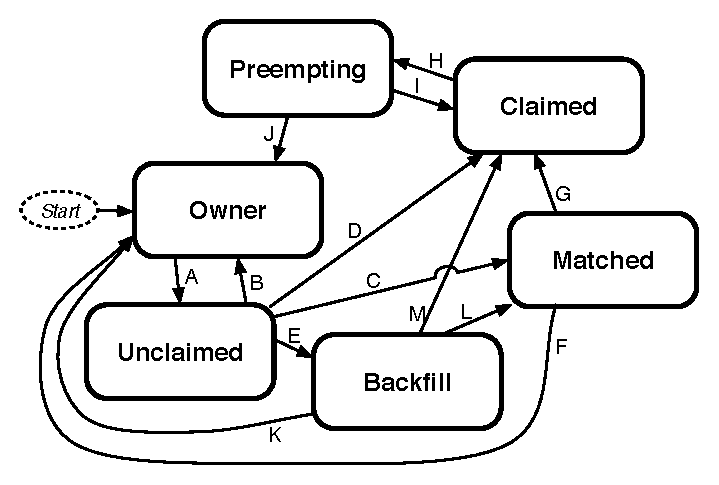
\includegraphics{admin-man/machine-states.eps}
\caption{\label{fig:machine-states}Machine States}
\end{figure}

%%%%%%%%%%%%%%%%%%%%%%%%%%%%%%%%%%%%%%%%%%%%%%%%%%%%%%%%%%%%%%%%%%%%%%
\subsection{\label{sec:Activities}
Machine Activities}
%%%%%%%%%%%%%%%%%%%%%%%%%%%%%%%%%%%%%%%%%%%%%%%%%%%%%%%%%%%%%%%%%%%%%%

\index{machine activity}
\index{activity!of a machine}
Within some machine states,
\Term{activities} of the machine are defined.
The state has meaning regardless of activity.
Differences between activities are significant.
Therefore, a ``state/activity'' pair describes
a machine.
The following list describes all the possible state/activity pairs.

\begin{itemize}

\item Owner
\begin{description}
\index{machine activity!Idle}
\item[Idle] This is the only activity for Owner state.  As far as
  Condor is concerned the machine is Idle, since it is not doing
  anything for Condor.
\end{description}

\index{machine activity!Unclaimed}
\item Unclaimed
\begin{description}
\item[Idle] This is the normal activity of Unclaimed machines.
  The machine is still Idle in that the machine owner is willing to
  let Condor jobs run, but Condor is not using the
  machine for anything.
  
\index{machine activity!Benchmarking}
\item[Benchmarking] The machine is running benchmarks to
  determine the speed on this machine.
  This activity only occurs in the Unclaimed state.
  How often the activity occurs is
  determined by the \Expr{RunBenchmarks} expression.
\end{description}

\item Matched
\begin{description}
\item[Idle] When Matched, the machine is still Idle to Condor.
\end{description}

\item Claimed
\begin{description}
\item[Idle] In this activity, the machine has been claimed, but the
  schedd that claimed it has yet to \Term{activate} the claim by
  requesting a \Condor{starter} to be spawned to service a job.
  
\index{machine activity!Busy}
\item[Busy] Once a \Condor{starter} has been started and the claim is
  active, the machine moves to the Busy activity to signify that it is
  doing something as far as Condor is concerned.
  
\index{machine activity!Suspended}
\item[Suspended] If the job is suspended by Condor, the machine goes
  into the Suspended activity.
  The match between the schedd and machine has not been broken (the
  claim is still valid), but the job is not making any progress and
  Condor is no longer generating a load on the machine.
\end{description}

\item Preempting
  The preempting state is used for evicting a Condor job from a given
  machine.
  When the machine enters the Preempting state, it checks the
  \Expr{WANT\_VACATE} expression to determine its activity.

\begin{description}
\index{machine activity!Vacating}
\item[Vacating] In the Vacating activity, the job that was running is
  in the process of checkpointing.
  As soon as the checkpoint process completes,
  the machine moves into either the Owner state or the
  Claimed state, depending on the reason for its preemption.
  
\index{machine activity!Killing}
\item[Killing] Killing means that the machine has requested the running
  job to exit the machine immediately, without checkpointing.
\end{description}

\end{itemize}

Figure~\ref{fig:machine-activities} on
page~\pageref{fig:machine-activities} gives the overall view of all
machine states and activities and shows the possible transitions
from one to another within the Condor system.  
Each transition is labeled with a number on the diagram, and
transition numbers referred to in this manual will be \Bold{bold}.  

\index{machine state and activities figure}
\index{state and activities figure}
\index{activities and state figure}
\begin{figure}[hbt]
\centering
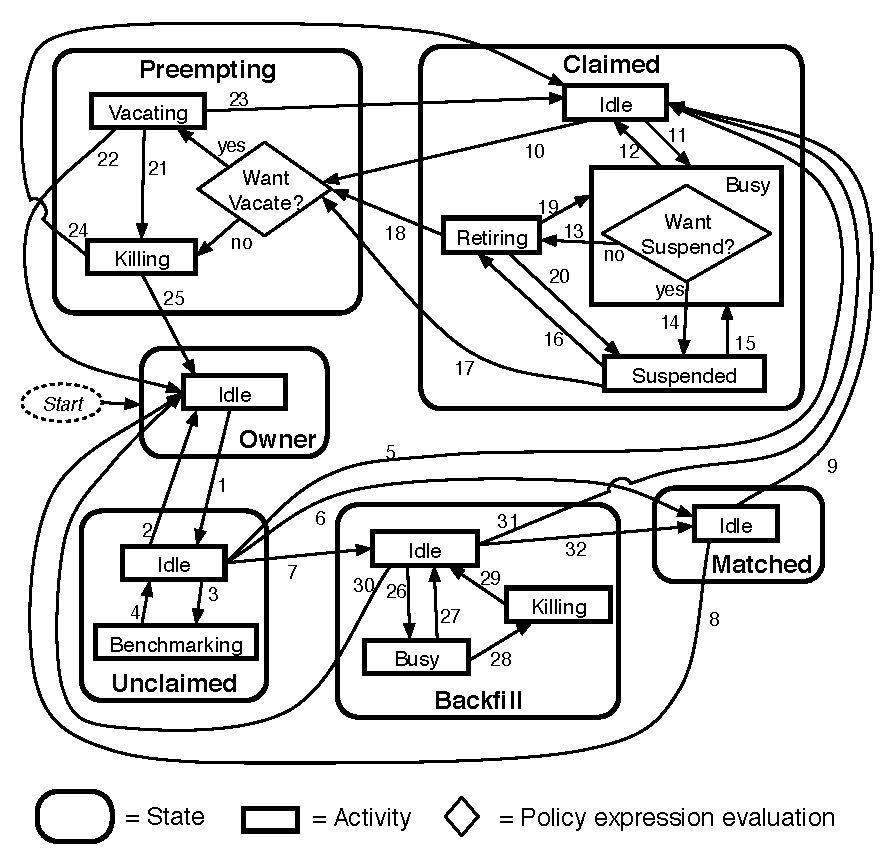
\includegraphics{admin-man/machine-activities.eps}
\caption{\label{fig:machine-activities}Machine States and Activities}
\end{figure}

Various expressions are used to determine when and if many of these
state and activity transitions occur.  Other transitions are initiated
by parts of the Condor protocol (such as when the \Condor{negotiator}
matches a machine with a schedd).  The following section describes the
conditions that lead to the various state and activity transitions.

%%%%%%%%%%%%%%%%%%%%%%%%%%%%%%%%%%%%%%%%%%%%%%%%%%%%%%%%%%%%%%%%%%%%%%
\subsection{\label{sec:State-and-Activity-Transitions}
State and Activity Transitions}
%%%%%%%%%%%%%%%%%%%%%%%%%%%%%%%%%%%%%%%%%%%%%%%%%%%%%%%%%%%%%%%%%%%%%%

\index{machine state!transitions|(}
\index{machine activity!transitions|(}
\index{state!transitions|(}
\index{activity!transitions|(}
This section traces through all possible state and activity
transitions within a machine and describes the conditions under which
each one occurs.
Whenever a transition occurs, Condor records when the machine entered its
new activity and/or new state.
These times are often used to write expressions that determine
when further transitions occurred.
For example, enter the Killing activity if a machine has been in
the Vacating activity longer than a specified amount of time. 

%%%%%%%%%%%%%%%%%%%%%%%%%%%%%%%%%%%%%%%%%%%%%%%%%%%%%%%%%%%%%%%%%%%%%%
\subsubsection{\label{sec:Owner-State}
Owner State}
%%%%%%%%%%%%%%%%%%%%%%%%%%%%%%%%%%%%%%%%%%%%%%%%%%%%%%%%%%%%%%%%%%%%%%

\index{expression!\Expr{IsOwner}}
\index{IsOwner@\Expr{IsOwner} expression}
\index{configuration!IsOwner@\Expr{IsOwner} expression}
When the startd is first spawned, the machine it represents enters the
Owner state. 
The machine remains in the Owner state while the
expression \Expr{IsOwner} is TRUE.
If the \Expr{IsOwner} expression is FALSE,
then the machine transitions to the Unclaimed state.
The default value for the 
\Expr{IsOwner} expression is optimized for a shared resource
\begin{verbatim}
START =?= FALSE
\end{verbatim}
So,
the machine will remain in the Owner state as long as the \Expr{START}
expression locally evaluates to FALSE.
Section~\ref{sec:Start-Expr} provides more detail on the
\Expr{START} expression.
If the \Expr{START} locally evaluates to TRUE or cannot be locally
evaluated (it evaluates to UNDEFINED), transition \Bold{1}
occurs and the machine enters the Unclaimed state.
The \Expr{IsOwner} expression is locally evaluated by the machine,
and should not reference job ClassAd attributes, which would be
UNDEFINED.

For dedicated resources, the recommended value for the \Expr{IsOwner}
expression is FALSE.

The Owner state represents a resource that is in use by its
interactive owner (for example, if the keyboard is being used).
The Unclaimed state represents a resource that is neither in use by
its interactive user, nor the Condor system.
From Condor's point of view, there is little difference between the
Owner and Unclaimed states.
In both cases, the resource is not currently in use by the Condor
system.
However, if a job matches the resource's \Expr{START} expression, the
resource is available to run a job, regardless of if it is in the
Owner or Unclaimed state.
The only differences between the two states are how the resource shows
up in \Condor{status} and other reporting tools, and the fact that
Condor will not run benchmarking on a resource in the Owner state.
As long as the \Expr{IsOwner} expression is TRUE, the machine is
in the Owner State.
When the \Expr{IsOwner} expression is FALSE, the machine goes into
the Unclaimed State.

Here is an example that assumes that an \Expr{IsOwner}
expression is not present in the configuration.
If the \Expr{START} expression is
\begin{verbatim}
START = KeyboardIdle > 15 * $(MINUTE) && Owner == "coltrane" 
\end{verbatim}
and if \Attr{KeyboardIdle} is 34 seconds,
then the machine would remain in the Owner state.
Owner is undefined, and
\verb@anything && FALSE@ is FALSE.

If, however, the \Expr{START} expression is
\begin{verbatim}
        START = KeyboardIdle > 15 * $(MINUTE) || Owner == "coltrane"
\end{verbatim}
and \Attr{KeyboardIdle} is 34 seconds, then the machine
leaves the Owner state and becomes Unclaimed.
This is because
\verb@FALSE || UNDEFINED@ is UNDEFINED.
So, while this machine is not available to just anybody,
if user coltrane has jobs submitted, the machine is willing to run them.
Any other user's jobs have to wait
until \Attr{KeyboardIdle} exceeds 15 minutes.
However, since coltrane might claim this resource,
but has not yet, the machine goes to the Unclaimed state.

While in the Owner state, the startd polls the status of the
machine every \Macro{UPDATE\_INTERVAL} to see if anything has changed
that would lead it to a different state.
This minimizes the impact on the Owner
while the Owner is using the machine.
Frequently waking up, computing load averages, checking the access
times on files, computing free swap space take time,
and there is nothing
time critical that the startd needs to be sure to notice as soon as it
happens.
If the \Expr{START} expression evaluates to TRUE and five
minutes pass before the startd notices,
that's a drop in the bucket of high-throughput computing.

The machine can only transition to the Unclaimed state from the Owner state.
It only does so when the \Expr{START} expression no longer locally
evaluates to FALSE.
In general, if the \Expr{START}
expression locally evaluates to FALSE at any time,
the machine will either transition directly to the Owner state
or to the Preempting state on its way to the Owner state,
if there is a job running that needs preempting.

%%%%%%%%%%%%%%%%%%%%%%%%%%%%%%%%%%%%%%%%%%%%%%%%%%%%%%%%%%%%%%%%%%%%%%
\subsubsection{\label{sec:Unclaimed-State}Unclaimed State}
%%%%%%%%%%%%%%%%%%%%%%%%%%%%%%%%%%%%%%%%%%%%%%%%%%%%%%%%%%%%%%%%%%%%%%

If the \Expr{IsOwner} expression becomes TRUE, then the machine returns
to the Owner state.
If the \Expr{IsOwner} expression becomes FALSE, then the machine remains
in the Unclaimed state.
If the \Expr{IsOwner} expression is not present in the configuration files,
then the default value for the \Expr{IsOwner} expression is 
\begin{verbatim}
START =?= FALSE
\end{verbatim}
so that
while in the Unclaimed state, if the \Expr{START} expression locally
evaluates to FALSE, the machine returns to the Owner state by
transition \Bold{2}.

When in the Unclaimed state,
the \Expr{RunBenchmarks} \label{param:RunBenchmarks}  
expression is relevant.
If \Expr{RunBenchmarks} evaluates to TRUE while the machine
is in the Unclaimed state,
then the machine will transition from the Idle
activity to the Benchmarking activity (transition \Bold{3}) and
perform benchmarks to determine \Attr{MIPS} and \Attr{KFLOPS}.  
When the benchmarks complete, the machine returns to the Idle activity
(transition \Bold{4}).

The startd automatically inserts an attribute, \Attr{LastBenchmark},
whenever it runs benchmarks, so commonly \Attr{RunBenchmarks} is
defined in terms of this attribute, for example:
\begin{verbatim}
        BenchmarkTimer = (CurrentTime - LastBenchmark)
        RunBenchmarks = $(BenchmarkTimer) >= (4 * $(HOUR))
\end{verbatim}
Here, a macro, \MacroNI{BenchmarkTimer} is defined to help write the
expression.
This macro holds the time since the last benchmark,
so when this time exceeds 4 hours, we run the benchmarks again.
The startd keeps a weighted average of these benchmarking
results to try to get the most accurate numbers possible.
This is why
it is desirable for 
the startd to run them more than once in its lifetime.

\Note \Attr{LastBenchmark} is initialized to 0 before benchmarks
have ever been run.
So, if you want the startd to run benchmarks as soon as the machine is
Unclaimed (if it hasn't done so already),
include a term for \Attr{LastBenchmark} as in the example above.

\Note If \Expr{RunBenchmarks} is defined and set to something
other than FALSE, the startd will automatically run one set of
benchmarks when it first starts up.
To disable benchmarks, both at startup and at any time thereafter,
set \Expr{RunBenchmarks} to FALSE or comment it out of the
configuration file.

From the Unclaimed state, the machine can go to three other possible
states: Owner (transition \Bold{2}), Matched, or Claimed/Idle.
Once the \Condor{negotiator} matches an Unclaimed machine with a
requester at a given schedd, the negotiator sends a command to both
parties, notifying them of the match.  
If the schedd receives that notification and initiates the claiming
procedure with the machine before the negotiator's message gets to the
machine, the Match state is skipped,
and the machine goes
directly to the Claimed/Idle state (transition \Bold{5}).
However, normally the machine will enter the Matched state (transition
\Bold{6}), even if it is only for a brief period of time.

%%%%%%%%%%%%%%%%%%%%%%%%%%%%%%%%%%%%%%%%%%%%%%%%%%%%%%%%%%%%%%%%%%%%%%
\subsubsection{\label{sec:Matched-State}Matched State}
%%%%%%%%%%%%%%%%%%%%%%%%%%%%%%%%%%%%%%%%%%%%%%%%%%%%%%%%%%%%%%%%%%%%%%

The Matched state is not very interesting to Condor.
Noteworthy in this state is that the machine lies about its \Expr{START}
expression while in this state and says that \Expr{Requirements} are
false to prevent being matched again before it has been claimed.
Also interesting is that
the startd starts a timer to make sure it does not stay in the
Matched state too long.
The timer is set with the \Macro{MATCH\_TIMEOUT}
\label{param:MatchTimeout} configuration file macro.
It is specified in seconds and defaults to 300 (5 minutes).
If the schedd that was matched with this machine does not
claim it within this period of time, the machine gives up,
and goes back into the Owner state via transition \Bold{7}.
It will probably leave the Owner state right away for the
Unclaimed state again and wait for another match. 

At any time while the machine is in the Matched state, if the
\Expr{START} expression locally evaluates to FALSE, the machine enters
the Owner state directly (transition \Bold{7}).

If the schedd that was matched with the machine claims it before the
\Macro{MATCH\_TIMEOUT} expires, the machine goes into the Claimed/Idle
state (transition \Bold{8}).

%%%%%%%%%%%%%%%%%%%%%%%%%%%%%%%%%%%%%%%%%%%%%%%%%%%%%%%%%%%%%%%%%%%%%%
\subsubsection{\label{sec:Claimed-State}Claimed State}
%%%%%%%%%%%%%%%%%%%%%%%%%%%%%%%%%%%%%%%%%%%%%%%%%%%%%%%%%%%%%%%%%%%%%%

The Claimed state is certainly the most complex state.
It has the most possible activities and the most expressions that
determine its next activities.
In addition, the \Condor{checkpoint} and \Condor{vacate} commands affect
the machine when it is in the Claimed state.
In general, there are two sets of expressions that might take effect.
They depend on the universe of the request: standard or vanilla.
The standard universe expressions are the normal expressions.
For example:
\begin{verbatim}
        WANT_SUSPEND            = True
        WANT_VACATE             = $(ActivationTimer) > 10 * $(MINUTE)
        SUSPEND                 = $(KeyboardBusy) || $(CPUBusy)
        ...
\end{verbatim}

The vanilla expressions have the string``\_VANILLA'' appended to their names.
For example:
\begin{verbatim}
        WANT_SUSPEND_VANILLA    = True
        WANT_VACATE_VANILLA     = True
        SUSPEND_VANILLA         = $(KeyboardBusy) || $(CPUBusy)
        ...
\end{verbatim}

Without specific vanilla versions, the normal versions
will be used for all jobs, including vanilla jobs.  
In this manual, the normal expressions are referenced.
The difference exists for the
the resource owner that might want the machine
to behave differently for vanilla jobs, since they cannot checkpoint.
For example, owners may want vanilla jobs to remain suspended for
longer than standard jobs.

While Claimed, the \Macro{POLLING\_INTERVAL} takes effect, and the
startd polls the machine much more frequently to evaluate its
state.

If the machine owner starts typing on the console again,
it is best to notice this as
soon as possible to be able to start doing whatever 
the machine owner wants at that point.
For SMP machines, if any virtual machine is in the Claimed state, the
startd polls the machine frequently.
If already polling one virtual machine, it does not
cost much to evaluate the state of all the virtual machines at
the same time.

In general, when the startd is going to take a job off a machine
(usually because of activity on the machine that signifies that the
owner is using the machine again),
the startd will go through
successive levels of getting the job out of the way.
The first and least costly to the job is suspending it.
This works for both standard and vanilla jobs.
If suspending the job for a short while does not satisfy the machine
owner (the owner is still using the machine after a specific period of
time), the startd moves on to vacating the job.
Vacating a standard universe job
involves performing a checkpoint so that the work already completed
is not lost.  Vanilla jobs are sent a \Term{softkill signal} so that they
can gracefully shutdown if necessary; the default is \verb@SIGTERM@.
If vacating does not satisfy the machine owner (usually because it is
taking too long and the owner wants their machine back \emph{now}),
the final, most drastic stage is reached: killing.  
Killing is a quick death to the job, using a hard-kill signal that cannot
be intercepted by the application.  For vanilla jobs that do no special
signal handling, vacating and killing are equivalent.

The \Expr{WANT\_SUSPEND} expression determines if the machine will
evaluate the \Expr{SUSPEND} expression to consider entering the
Suspended activity.
The \Expr{WANT\_VACATE} expression determines what happens when the
machine enters the Preempting state.
It will go to the Vacating
activity or directly to Killing. 
If one or both of these expressions evaluates to FALSE, the machine
will skip that stage of getting rid of the job and proceed directly to
the more drastic stages.

When the machine first enters the Claimed state, it goes to the Idle
activity.  From there, it has two options.  
It can enter the Preempting state via transition \Bold{9} (if a 
\Condor{vacate} arrives, or if the \Expr{START} expression locally
evaluates to FALSE),  
or it can enter the Busy activity (transition \Bold{10}) if the
schedd that has claimed the machine decides to activate the claim and
start a job.

From Claimed/Busy, the machine can transition to three other state/activity
pairs.
The startd evaluates the \Expr{WANT\_SUSPEND} expression to decide
which other expressions to evaluate.  
If \Expr{WANT\_SUSPEND} is TRUE, then the startd evaluates the
\Expr{SUSPEND} expression.
If \Expr{WANT\_SUSPEND} is FALSE, then the startd will
evaluate the \Expr{PREEMPT} expression and skip the Suspended activity
entirely.
By transition, the possible state/activity destinations from Claimed/Busy:

\begin{description}
  
\item[Claimed/Idle] If the starter that is serving a given job exits
  (for example because the jobs completes), the machine will go
  to Claimed/Idle (transition \Bold{11}).
  
\item[Preempting] If \Expr{WANT\_SUSPEND} is FALSE and the
  \Expr{PREEMPT} expression is TRUE, the machine enters the
  Preempting state (transition \Bold{12}).
  The other reason the machine would go from Claimed/Busy to
  Preempting is if the \Condor{negotiator} matched the machine
  with a ``better'' match.  This better match could either be from the
  machine's perspective using the \Expr{RANK} Expression above,
  or it could be from the negotiator's perspective due to
  a job with a higher user priority.
  In this case, \Expr{WANT\_VACATE} is assumed to be TRUE, and the
  machine transitions to Preempting/Vacating.
  
\item[Claimed/Suspended] If both the \Expr{WANT\_SUSPEND} and
  \Expr{SUSPEND} expressions evaluate to TRUE, the machine
  suspends the job (transition \Bold{13}).
  
\end{description}
  
If a \Condor{checkpoint} command arrives,
or the \Expr{PeriodicCheckpoint} expression evaluates to TRUE,
there is no state change.
The startd has no way of knowing when this process completes,
so periodic checkpointing can not be another state.
Periodic checkpointing remains in the Claimed/Busy state
and appears as a running job.

From the Claimed/Suspended state, the following transitions
may occur:

\begin{description}
  
\item[Claimed/Busy] If the \Expr{CONTINUE} expression evaluates to
  TRUE, the machine resumes the job and enters the
  Claimed/Busy state (transition \Bold{14}).

\item[Preempting] If the \Expr{PREEMPT} expression is TRUE, the machine
  will enter the Preempting state (transition \Bold{15}).

\end{description}

%%%%%%%%%%%%%%%%%%%%%%%%%%%%%%%%%%%%%%%%%%%%%%%%%%%%%%%%%%%%%%%%%%%%%%
\subsubsection{\label{sec:Preempting-State}Preempting State}
%%%%%%%%%%%%%%%%%%%%%%%%%%%%%%%%%%%%%%%%%%%%%%%%%%%%%%%%%%%%%%%%%%%%%%

The Preempting state is less complex than the Claimed state.
There are two activities.
Depending on the value of \Expr{WANT\_VACATE}, a machine will
be in the
Vacating activity (if TRUE) or the Killing activity (if FALSE).  

While in the Preempting state (regardless of activity) the machine
advertises its \Expr{Requirements} expression as FALSE to signify that
it is not available for further matches, either because it is about to
transition
to the Owner state, or because it has already been matched with
one preempting match, and further preempting matches are disallowed
until the machine has been claimed by the new match.

The main function of the Preempting state is to get rid of the starter
associated with the resource.  If the \Condor{starter} associated with
a given claim exits while the machine is still in the Vacating
activity, then the job successfully completed a graceful shutdown.
For standard universe jobs, this means that a checkpoint was saved.
For other jobs, this means the application was given an opportunity to
do a graceful shutdown, by intercepting the soft kill signal.

If the machine is in the Vacating activity, it keeps evaluating the 
\Expr{KILL} expression.
As soon as this expression evaluates to TRUE,
the machine enters the Killing activity (transition \Bold{16}).

When the starter exits, or if there was no starter running when the
machine enters the Preempting state (transition \Bold{9}),
the other purpose of the Preempting state is completed:
notifying the schedd that had claimed this machine that the claim is
broken.

At this point, the machine enters either the Owner state by
transition \Bold{17} (if the job was preempted because the machine
owner came back) or the Claimed/Idle state by transition \Bold{18}
(if the job was preempted because a better match was found).
The machine enters the Killing activity, and it starts a timer, the
length of which is defined by the \Macro{KILLING\_TIMEOUT}
\label{param:KillingTimeout} macro.
This macro is defined in seconds and defaults to 30.
If this timer expires and the machine is still in
the Killing activity, something has gone seriously wrong with the
\Condor{starter} and the startd tries to vacate the job immediately by
sending SIGKILL to all of the \Condor{starter}'s children, and then to
the \Condor{starter} itself.

Once the starter is gone and the schedd that had claimed the
machine is notified that the claim is broken, the machine will either
enter the Owner state by transition \Bold{19} (if the job was
preempted because the machine owner came back) or the Claimed/Idle
state by transition \Bold{20} (if the job was preempted because a
better match was found). 

%%%%%%%%%%%%%%%%%%%%%%%%%%%%%%%%%%%%%%%%%%%%%%%%%%%%%%%%%%%%%%%%%%%%%%
\subsection{\label{sec:State-Expression-Summary}
State/Activity Transition Expression Summary}
%%%%%%%%%%%%%%%%%%%%%%%%%%%%%%%%%%%%%%%%%%%%%%%%%%%%%%%%%%%%%%%%%%%%%%
\index{machine state!transitions summary}
\index{machine activity!transitions summary}
\index{state!transitions summary}
\index{activity!transitions summary}
This section is a summary of the information from the
previous sections.
It serves as a quick reference.

\begin{description}
  
\item[\Expr{START}] When TRUE, the machine is willing to spawn
  a remote Condor job.
  
\item[\Expr{RunBenchmarks}] While in the Unclaimed state, the machine
  will run benchmarks whenever TRUE.
  
\item[\Macro{MATCH\_TIMEOUT}] If the machine has been in the Matched
  state longer than this value, it will transition to the Owner state.
  
\item[\Expr{WANT\_SUSPEND}] If TRUE, the machine evaluates
  the \Expr{SUSPEND} expression to see if it should transition to the
  Suspended activity.  If FALSE, the machine look at
  the \Expr{PREEMPT} expression.
  
\item[\Expr{SUSPEND}] If \Expr{WANT\_SUSPEND} is TRUE, and the machine
  is in the Claimed/Busy state, it enters the Suspended activity
  if \Expr{SUSPEND} is TRUE.
  
\item[\Expr{CONTINUE}] If the machine is in the Claimed/Suspended
  state, it enter the Busy activity if \Expr{CONTINUE} is TRUE.
  
\item[\Expr{PREEMPT}] If the machine is either in the Claimed/Suspended
  activity, or is in the Claimed/Busy activity and
  \Expr{WANT\_SUSPEND} is FALSE, the machine enters the Preempting
  state whenever \Expr{PREEMPT} is TRUE. 
  
\item[\Expr{WANT\_VACATE}] This is checked only when the
  \Expr{PREEMPT} expression is TRUE and the machine enters the
  Preempting state.
  If \Expr{WANT\_VACATE} is TRUE, the machine enters the Vacating
  activity.  
  If it is FALSE, the machine will proceed directly to the Killing
  activity.  
  
\item[\Expr{KILL}] If the machine is the Preempting/Vacating state, it
  enters Preempting/Killing whenever \Expr{KILL} is TRUE. 
  
\item[\Macro{KILLING\_TIMEOUT}] If the machine is in the
  Preempting/Killing state for longer than \Macro{KILLING\_TIMEOUT}
  seconds, the startd sends a SIGKILL to the \Condor{starter}
  and all its children to try to kill the job as quickly as possible.
  
\item[\Expr{PERIODIC\_CHECKPOINT}] If the machine is in the
  Claimed/Busy state and \Expr{PERIODIC\_CHECKPOINT} is TRUE, the
  user's job begins a periodic checkpoint.
  
\item[\Expr{RANK}] If this expression evaluates to a higher number for
  a pending resource request than it does for the current request, the
  machine preempts the current request (enters the
  Preempting/Vacating state).  When the preemption is complete, the
  machine enters the Claimed/Idle state with the new resource
  request claiming it.

\end{description}
\index{machine state!transitions|)}
\index{machine activity!transitions|)}
\index{state!transitions|)}
\index{activity!transitions|)}

%%%%%%%%%%%%%%%%%%%%%%%%%%%%%%%%%%%%%%%%%%%%%%%%%%%%%%%%%%%%%%%%%%%%%%
\subsection{\label{sec:Policy-Settings}Policy Settings}
%%%%%%%%%%%%%%%%%%%%%%%%%%%%%%%%%%%%%%%%%%%%%%%%%%%%%%%%%%%%%%%%%%%%%%

This section describes the default configuration
policy and then provides examples of extensions to these
policies.

%%%%%%%%%%%%%%%%%%%%%%%%%%%%%%%%%%%%%%%%%%%%%%%%%%%%%%%%%%%%%%%%%%%%%%
\subsubsection{\label{sec:Default-Policy}Default Policy Settings}
%%%%%%%%%%%%%%%%%%%%%%%%%%%%%%%%%%%%%%%%%%%%%%%%%%%%%%%%%%%%%%%%%%%%%%

\index{policy!default with Condor}
\index{Condor!default policy}
These settings are the default as shipped with Condor.  They have been
used for many years with no problems.  The vanilla expressions are
identical to the regular ones. (They are not listed here.  If
not defined, the standard expressions are used for vanilla jobs
as well).

The following are macros to help write the expressions
clearly.

\begin{description}
  
\item[\Macro{StateTimer}] Amount of time in the current state.

\item[\Macro{ActivityTimer}] Amount of time in the current activity. 

\item[\Macro{ActivationTimer}] Amount of time the job has been running on
  this machine.

\item[\Macro{LastCkpt}] Amount of time since the last periodic checkpoint.

\item[\Macro{NonCondorLoadAvg}] The difference between the system load and
  the Condor load (the load generated by everything but Condor).

\item[\Macro{BackgroundLoad}] Amount of background load permitted
  on the machine and still start a Condor job.

\item[\Macro{HighLoad}] If the \MacroU{NonCondorLoadAvg} goes over
  this, the CPU is considered too busy, and eviction of the Condor
  job should start. 

\item[\Macro{StartIdleTime}] Amount of time the keyboard must to be idle
  before Condor will start a job.

\item[\Macro{ContinueIdleTime}] Amount of time the keyboard must to be idle
  before resumption of a suspended job.

\item[\Macro{MaxSuspendTime}] Amount of time a job may be
  suspended before more drastic measures are taken.

\item[\Macro{MaxVacateTime}] Amount of time a job may be
  checkpointing before we give up and kill it outright.

\item[\Macro{KeyboardBusy}] A boolean expression that evaluates to TRUE
    when the keyboard is being used.

\item[\Macro{CPUIdle}] A boolean expression that evaluates to TRUE
    when the CPU is idle.

\item[\Macro{CPUBusy}] A boolean expression that evaluates
    to TRUE when the CPU is busy.

\item[\Macro{MachineBusy}] The CPU or the Keyboard is busy.

\item[\Macro{CPUIsBusy}] A boolean value set to the same value as 
    \Macro{CPUBusy}.

\item[\Macro{CPUBusyTime}] The value 0 if \Macro{CPUBusy}
    is False; the time in seconds since
    \Macro{CPUBusy} became True.
    
\end{description}

\begin{verbatim}
##  These macros are here to help write legible expressions:
MINUTE          = 60
HOUR            = (60 * $(MINUTE))
StateTimer      = (CurrentTime - EnteredCurrentState)
ActivityTimer   = (CurrentTime - EnteredCurrentActivity)
ActivationTimer = (CurrentTime - JobStart)
LastCkpt        = (CurrentTime - LastPeriodicCheckpoint)

NonCondorLoadAvg        = (LoadAvg - CondorLoadAvg)
BackgroundLoad          = 0.3
HighLoad                = 0.5
StartIdleTime           = 15 * $(MINUTE)
ContinueIdleTime        = 5 * $(MINUTE)
MaxSuspendTime          = 10 * $(MINUTE)
MaxVacateTime           = 10 * $(MINUTE)

KeyboardBusy            = KeyboardIdle < $(MINUTE)
ConsoleBusy             = (ConsoleIdle  < $(MINUTE))
CPUIdle                = $(NonCondorLoadAvg) <= $(BackgroundLoad)
CPUBusy                = $(NonCondorLoadAvg) >= $(HighLoad)
KeyboardNotBusy         = ($(KeyboardBusy) == False)
MachineBusy             = ($(CPUBusy) || $(KeyboardBusy)
\end{verbatim}

Macros are defined to want to suspend jobs (instead of
killing them) in the case of jobs that use little memory,
when the keyboard is not being used, and for vanilla universe
and PVM universe jobs.
We want to gracefully vacate jobs which
have been running for more than 10 minutes
or are vanilla universe or PVM universe jobs.
\begin{verbatim}
WANT_SUSPEND       = ( $(SmallJob) || $(KeyboardNotBusy) \
                       || $(IsPVM) || $(IsVanilla) )
WANT_VACATE        = ( $(ActivationTimer) > 10 * $(MINUTE) \
                       || $(IsPVM) || $(IsVanilla) )
\end{verbatim}

Finally, definitions of the actual expressions.
Start a job if 
the keyboard has been idle long enough and
the load average is low enough OR the machine is currently
running a Condor job.
Note that Condor would only run one job at a time.
It just may prefer to run a different job, as defined by
the machine rank or user priorities.
\begin{verbatim}
START        = ( (KeyboardIdle > $(StartIdleTime)) \
                  && ( $(CPUIdle) || \
                       (State != "Unclaimed" && State != "Owner")) )
\end{verbatim}

Suspend a job if the keyboard has been touched.
Alternatively, suspend if the CPU has been busy for more than two minutes
and the job has been running for more than 90 seconds.
\begin{verbatim}
SUSPEND         = ( $(KeyboardBusy) || \
                 ( (CpuBusyTime > 2 * $(MINUTE)) \
                    && $(ActivationTimer) > 90 ) )
\end{verbatim}

Continue a suspended job if the CPU is idle, the Keyboard has been
idle for long enough, and the job has been suspended more
than 10 seconds.
\begin{verbatim}
CONTINUE        = ( $(CPUIdle) && ($(ActivityTimer) > 10) \
                  && (KeyboardIdle > $(ContinueIdleTime)) )
\end{verbatim}

There are two conditions that signal preemption.
The first condition is if the job is suspended,
but it has been suspended too long.
The second condition is if suspension is not desired and the machine is busy. 
\begin{verbatim}
PREEMPT	        = ( ((Activity == "Suspended") && \
                    ($(ActivityTimer) > $(MaxSuspendTime))) \
                    || (SUSPEND && (WANT_SUSPEND == False)) )
\end{verbatim}

Kill jobs that take too long leaving gracefully.
\begin{verbatim}
KILL            = $(ActivityTimer) > $(MaxVacateTime)
\end{verbatim}

Finally, specify periodic checkpointing.  
For jobs smaller than 60 Mbytes, do a periodic checkpoint every 6 hours.  
For larger jobs, only checkpoint every 12 hours.
\begin{verbatim}
PERIODIC_CHECKPOINT     = ( (ImageSize < 60000) && \
                            ($(LastCkpt) > (6 * $(HOUR))) ) || \ 
                          ( $(LastCkpt) > (12 * $(HOUR)) )
\end{verbatim}

\index{policy!at UW-Madison}

At UW-Madison, we have a fast network.
We simplify our expression considerably to
\begin{verbatim}
PERIODIC_CHECKPOINT     = $(LastCkpt) > (3 * $(HOUR))
\end{verbatim}

For reference, the entire set of policy settings are included
once more without comments:

\begin{verbatim}
##  These macros are here to help write legible expressions:
MINUTE          = 60
HOUR            = (60 * $(MINUTE))
StateTimer      = (CurrentTime - EnteredCurrentState)
ActivityTimer   = (CurrentTime - EnteredCurrentActivity)
ActivationTimer = (CurrentTime - JobStart)
LastCkpt        = (CurrentTime - LastPeriodicCheckpoint)

NonCondorLoadAvg        = (LoadAvg - CondorLoadAvg)
BackgroundLoad          = 0.3
HighLoad                = 0.5
StartIdleTime           = 15 * $(MINUTE)
ContinueIdleTime        = 5 * $(MINUTE)
MaxSuspendTime          = 10 * $(MINUTE)
MaxVacateTime           = 10 * $(MINUTE)

KeyboardBusy            = KeyboardIdle < $(MINUTE)
ConsoleBusy             = (ConsoleIdle  < $(MINUTE))
CPUIdle                = $(NonCondorLoadAvg) <= $(BackgroundLoad)
CPUBusy                = $(NonCondorLoadAvg) >= $(HighLoad)
KeyboardNotBusy         = ($(KeyboardBusy) == False)
MachineBusy             = ($(CPUBusy) || $(KeyboardBusy)

WANT_SUSPEND       = ( $(SmallJob) || $(KeyboardNotBusy) \
                       || $(IsPVM) || $(IsVanilla) )
WANT_VACATE        = ( $(ActivationTimer) > 10 * $(MINUTE) \
                       || $(IsPVM) || $(IsVanilla) )
START        = ( (KeyboardIdle > $(StartIdleTime)) \
                  && ( $(CPUIdle) || \
                       (State != "Unclaimed" && State != "Owner")) )
SUSPEND         = ( $(KeyboardBusy) || \
                 ( (CpuBusyTime > 2 * $(MINUTE)) \
                    && $(ActivationTimer) > 90 ) )
CONTINUE        = ( $(CPUIdle) && ($(ActivityTimer) > 10) \
                  && (KeyboardIdle > $(ContinueIdleTime)) )
PREEMPT	        = ( ((Activity == "Suspended") && \
                    ($(ActivityTimer) > $(MaxSuspendTime))) \
                    || (SUSPEND && (WANT_SUSPEND == False)) )
KILL            = $(ActivityTimer) > $(MaxVacateTime)
PERIODIC_CHECKPOINT     = ( (ImageSize < 60000) && \
                            ($(LastCkpt) > (6 * $(HOUR))) ) || \ 
                          ( $(LastCkpt) > (12 * $(HOUR)) )
\end{verbatim}

%%%%%%%%%%%%%%%%%%%%%%%%%%%%%%%%%%%%%%%%%%%%%%%%%%%%%%%%%%%%%%%%%%%%%%
\subsubsection{\label{sec:Test-job Policy Example}
Test-job Policy Example}
%%%%%%%%%%%%%%%%%%%%%%%%%%%%%%%%%%%%%%%%%%%%%%%%%%%%%%%%%%%%%%%%%%%%%%

This example shows how the default macros can be used to
set up a machine for running test jobs from a specific user.
Suppose we want the machine to
behave normally, except if user coltrane submits a job.
In that case, we
want that job to start regardless of what is happening on the machine.
We do not want the job suspended, vacated or killed.
This is reasonable if 
we know coltrane is submitting very short
running programs for testing purposes. 
The jobs should be executed right away.
This works with any machine
(or the whole pool, for that matter) by adding the following 5 expressions
to the existing configuration:
\begin{verbatim}
        START      = ($(START)) || Owner == "coltrane"
        SUSPEND    = ($(SUSPEND)) && Owner != "coltrane"
        CONTINUE   = $(CONTINUE)
        PREEMPT    = ($(PREEMPT)) && Owner != "coltrane"
        KILL       = $(KILL)
\end{verbatim}
Notice that there is nothing special in either the
\Expr{CONTINUE} or \Expr{KILL} expressions.
If Coltrane's jobs never suspend, they never look at \Expr{CONTINUE}.  
Similarly, if they never preempt, they never look at \Expr{KILL}. 


%%%%%%%%%%%%%%%%%%%%%%%%%%%%%%%%%%%%%%%%%%%%%%%%%%%%%%%%%%%%%%%%%%%%%%
\subsubsection{\label{sec:Time of Day Policy}
Time of Day Policy}
%%%%%%%%%%%%%%%%%%%%%%%%%%%%%%%%%%%%%%%%%%%%%%%%%%%%%%%%%%%%%%%%%%%%%%

\index{policy!time of day}
Condor can be
configured to only run jobs at
certain times of the day.
In general, we discourage configuring a system like this, since you
can often get lots of good cycles out of machines, even when their
owners say ``I'm always using my machine during the day.''
However, if you submit mostly vanilla jobs or other jobs that cannot
checkpoint, it might be a good idea to only allow the jobs to run when
you know the machines will be idle and when they will not be
interrupted.

To configure this kind of policy, you should use the \Attr{ClockMin}
and \Attr{ClockDay} attributes, defined in
section~\ref{sec:Startd-Attributes} on ``Startd ClassAd Attributes''.
These are special attributes which are automatically inserted by the
\Condor{startd} into its ClassAd, so you can always reference them in
your policy expressions.
\Attr{ClockMin} defines the number of minutes that have passed since
midnight.  
For example, 8:00am is 8 hours after midnight, or 8 * 60 minutes, or
480.
5:00pm is 17 hours after midnight, or 17 * 60, or 1020.
\Attr{ClockDay} defines the day of the week, Sunday = 0, Monday = 1,
and so on.  

To make the policy expressions easy to read, we recommend using macros
to define the time periods when you want jobs to run or not run.  
For example, assume regular ``work hours'' at your site are from
8:00am until 5:00pm, Monday through Friday: 

\begin{verbatim}
WorkHours = ( (ClockMin >= 480 && ClockMin < 1020) && \
              (ClockDay > 0 && ClockDay < 6) ) 
AfterHours = ( (ClockMin < 480 || ClockMin >= 1020) || \
               (ClockDay == 0 || ClockDay == 6) )
\end{verbatim}

Of course, you can fine-tune these settings by changing the definition
of \Macro{AfterHours} and \Macro{WorkHours} for your site.

Assuming you are using the default policy expressions discussed above,
there are only a few minor changes required to force Condor jobs to
stay off of your machines during work hours:

\begin{verbatim}
# Only start jobs after hours.
START = $(AfterHours) && $(CPUIdle) && KeyboardIdle > $(StartIdleTime)

# Consider the machine busy during work hours, or if the keyboard or
# CPU are busy.
MachineBusy = ( $(WorkHours) || $(CPUBusy) || $(KeyboardBusy) )
\end{verbatim}

By default, the \Macro{MachineBusy} macro is used to define the
\Expr{SUSPEND} and \Expr{PREEMPT} expressions.  
If you have changed these expressions at your site, you will need to
add \MacroU{WorkHours} to your \Expr{SUSPEND} and \Expr{PREEMPT}
expressions as appropriate.  

Depending on your site, you might also want to avoid suspending jobs
during work hours, so that in the morning, if a job is running, it
will be immediately preempted, instead of being suspended for some
length of time:

\begin{verbatim}
WANT_SUSPEND = $(AfterHours)
\end{verbatim}

%%%%%%%%%%%%%%%%%%%%%%%%%%%%%%%%%%%%%%%%%%%%%%%%%%%%%%%%%%%%%%%%%%%%%%
\index{policy!desktop/non-desktop}
\index{preemption!desktop/non-desktop}
\subsubsection{\label{sec:Desktop/Non-Desktop Policy}
Desktop/Non-Desktop Policy}
%%%%%%%%%%%%%%%%%%%%%%%%%%%%%%%%%%%%%%%%%%%%%%%%%%%%%%%%%%%%%%%%%%%%%%

Suppose you have two classes of machines in your pool: desktop
machines and dedicated cluster machines.  In this case, you might not
want keyboard activity to have any effect on the dedicated machines.
For example, when you log into these machines to debug some problem,
you probably do not want a running job to suddenly be killed.  Desktop
machines, on the other hand, should do whatever is necessary to remain
responsive to the user.

There are many ways to achieve the desired behavior.  One way is to
make a standard desktop policy and a standard non-desktop policy and
to copy the desired one into the local configuration file for each
machine.  Another way is to define one standard policy (in
\condor{config}) with a simple toggle that can be set in the local
configuration file.  The following example illustrates the latter
approach.

For ease of use, an entire policy is included in this example.  Some of the
expressions are just the usual default settings.

\begin{verbatim}
# If "IsDesktop" is configured, make it an attribute of the machine ClassAd.
STARTD_EXPRS = IsDesktop

# Only consider starting jobs if:
# 1) the load average is low enough OR the machine is currently
#    running a Condor job
# 2) AND the user is not active (if a desktop)
START = ( ($(CPUIdle) || (State != "Unclaimed" && State != "Owner")) \
          && (IsDesktop =!= True || (KeyboardIdle > $(StartIdleTime))) )

# Suspend (instead of vacating/killing) for the following cases:
WANT_SUSPEND = ( $(SmallJob) || $(JustCpu) || $(IsPVM) \
                 || $(IsVanilla) )

# When preempting, vacate (instead of killing) in the following cases:
WANT_VACATE  = ( $(ActivationTimer) > 10 * $(MINUTE) \
                 || $(IsPVM) || $(IsVanilla) )

# Suspend jobs if:
# 1) The cpu has been busy for more than 1 minute, AND
# 2) the job has been running for more than 90 seconds
# 3) OR suspend if this is a desktop and the user is active
SUSPEND = ( ((CpuBusyTime > 2 * $(MINUTE)) && ($(ActivationTimer) > 90)) \
            || ( IsDesktop =?= True && $(KeyboardBusy) ) )

# Continue jobs if:
# 1) the cpu is idle, AND 
# 2) we've been suspended more than 5 minutes AND
# 3) the keyboard has been idle for long enough (if this is a desktop)
CONTINUE = ( $(CPUIdle) && ($(ActivityTimer) > 300) \
             && (IsDesktop =!= True || (KeyboardIdle > $(ContinueIdleTime))) )

# Preempt jobs if:
# 1) The job is suspended and has been suspended longer than we want
# 2) OR, we don't want to suspend this job, but the conditions to
#    suspend jobs have been met (someone is using the machine)
PREEMPT = ( ((Activity == "Suspended") && \
            ($(ActivityTimer) > $(MaxSuspendTime))) \
           || (SUSPEND && (WANT_SUSPEND == False)) )

# Kill jobs if they have taken too long to vacate gracefully
KILL = $(ActivityTimer) > $(MaxVacateTime) 

\end{verbatim}

With this policy in \condor{config}, the local configuration files for
desktops can be easily configured with the following line:

\begin{verbatim}
IsDesktop = True
\end{verbatim}

In all other cases, the default policy described above will ignore
keyboard activity.

%%%%%%%%%%%%%%%%%%%%%%%%%%%%%%%%%%%%%%%%%%%%%%%%%%%%%%%%%%%%%%%%%%%%%%
\index{policy!disabling preemption}
\index{preemption!disabling}
\subsubsection{\label{sec:Disabling Preemption}
Disabling Preemption}
%%%%%%%%%%%%%%%%%%%%%%%%%%%%%%%%%%%%%%%%%%%%%%%%%%%%%%%%%%%%%%%%%%%%%%

Preemption can result in jobs being killed by Condor.  When this
happens, the jobs remain in the queue and will be automatically
rescheduled.  We highly recommend designing jobs that work well in
this environment, rather than simply disabling preemption.

Planning for preemption makes jobs more robust in the face of other
sources of failure.  One way to live happily with preemption is to use
Condor's standard universe, which provides checkpointing.  If your job
is incompatible with the requirements of standard universe, you can
still have it gracefully shutdown and restart by intercepting the soft
kill signal.

All that being said, there still may be cases where you want to be
sure that Condor is never responsible for killing jobs.  This can be
achieved with the following policy:

\begin{verbatim}
PREEMPT = False
PREEMPTION_REQUIREMENTS = False
RANK = 0
\end{verbatim}

Setting \Macro{PREEMPT} to be false disables preemption from activity
on the machine (e.g. console activity from the machine owner).
\Macro{PREEMPTION\_REQUIREMENTS} is set to false to disable preemption
by users with better priority in the pool.  (Technically, that is part
of the negotiator policy, not the startd policy.)  Setting the
startd's \Macro{RANK} expression to 0 removes the possibility of
startd preemption, which is when the negotiator finds a job that the
startd likes better than the current job it is running.  For this
purpose, setting the rank to any constant or to nothing at all would
work just as well.

You should be aware of one disadvantage of this policy: A low priority
user can get a claim to a machine and then hold on to it indefinitely,
by running a very long job or by keeping the machine busy with a
continuous stream of short jobs.  The negotiator will not be able to
reallocate the resource to a higher priority user until the machine
returns to an unclaimed state.

%%%%%%%%%%%%%%%%%%%%%%%%%%%%%%%%%%%%%%%%%%%%%%%%%%%%%%%%%%%%%%%%%%%%%%
\subsection{\label{sec:V60-Policy-diffs}Differences from the 
Version 6.0 Policy Settings}
%%%%%%%%%%%%%%%%%%%%%%%%%%%%%%%%%%%%%%%%%%%%%%%%%%%%%%%%%%%%%%%%%%%%%%

\index{policy!version differences}
This section describes how the current policy expressions
differ from the policy expressions in previous versions of Condor.
If you have never used Condor version 6.0 or earlier, or you never looked
closely at the policy settings, skip this section.

In summary, there is no longer a \Macro{VACATE} expression, and the
\Macro{KILL} expression is not evaluated while a machine is claimed. 
There is a \Macro{PREEMPT} expression which describes the
conditions when a machine will move from the Claimed state to the
Preempting state.
Once a machine is transitioning into the Preempting state, the
\Macro{WANT\_VACATE} expression controls whether the job should
be vacated with a checkpoint or directly killed.
The \Macro{KILL} expression determines the transition from
Preempting/Vacating to Preempting/Killing.  

In previous versions of Condor,
the \Macro{KILL} expression handled three distinct cases
(the transitions from Claimed/Busy, Claimed/Suspended and
Preempting/Vacating), and the \Macro{VACATE} expression handled
two cases (the transitions from Claimed/Busy and Claimed/Suspended).
In the current version of Condor, \Macro{PREEMPT} handles the
same two cases as the previous \Macro{VACATE} expression,
but the \Macro{KILL} expression handles one case.
Very complex policies can now be specified using all of
the default expressions, only tuning the \Macro{WANT\_VACATE} and
\Macro{WANT\_SUSPEND} expressions.
In previous versions, heavy use of the \Macro{WANT\_*}
expressions caused a complex \Macro{KILL} expression.

%%%%%%%%%%%%%%%%%%%%%%%%%%%%%%%%%%%%%%%%%%%%%%%%%%%%%%%%%%%%%%%%%%%%%%%%%%%
\section{\label{sec:Security}Security In Condor}
%%%%%%%%%%%%%%%%%%%%%%%%%%%%%%%%%%%%%%%%%%%%%%%%%%%%%%%%%%%%%%%%%%%%%%%%%%%
\index{security! in Condor|(}

This section describes various aspects of security within Condor.

%%%%%%%%%%%%%%%%%%%%%%%%%%%%%%%%%%%%%%%%%%%%%%%%%%%%%%%%%%%%%%%%%%%%%%
\subsection{\label{sec:uids}UIDs in Condor}
%%%%%%%%%%%%%%%%%%%%%%%%%%%%%%%%%%%%%%%%%%%%%%%%%%%%%%%%%%%%%%%%%%%%%%

\index{UIDs in Condor|(}

On a Unix system,
UIDs (User IDentification numbers) form part of an operating system's
tools for maintaining access control.
Each executing program has a UID,
a unique identifier of a user executing the program.
This is also called the real UID.
\index{UID!real}
A common situation has one user executing the program owned
by another user.
Many system commands work this way, with a user (corresponding
to a person) executing a program belonging to (owned by) root.
Since the program may require privileges that root has which
the user does not have, a special bit in the program's
protection specification (a setuid bit) allows the program
to run with the UID of the program's owner, instead of the
user that executes the program.
This UID of the program's owner is called an effective UID.
\index{UID!effective}

%GID (group identification)
Condor works most smoothly when its daemons run as root.
The daemons then have the ability to switch their 
effective UIDs at will.
When the daemons run as root,
they normally leave their effective UID and GID (Group IDentification)
to be those of user and group \verb@condor@.
This allows access to the log files without
changing the ownership of the log files.
It also allows access to these files when
the user condor's home directory resides on an NFS server.
root can not normally access NFS files.

If there is no \verb@condor@ user and group on the system, an
administrator can specify which UID and GID the Condor daemons should
use when they do not need root privileges in two ways, 
either with the \Env{CONDOR\_IDS} environment variable or the
\Macro{CONDOR\_IDS} configuration file setting.
In either case, the value should be the UID integer, followed by a
period, followed by the GID integer.
For example, if a Condor administrator does not want to create a
\verb@condor@ user, and instead wants their Condor daemons to run as
the \verb@daemon@ user (a common non-root user for system daemons to
execute as), the \verb@daemon@ user's UID was 2, and group
\verb@daemon@ had a GID of 2, the corresponding setting in the Condor
configuration file would be \verb@CONDOR_IDS = 2.2@.

On a machine where a job is submitted,
the \Condor{schedd} daemon
changes its effective UID to root
such that it has the capability to start up a \Condor{shadow} daemon
for the job.
Before a \Condor{shadow} daemon is created,
the \Condor{schedd} daemon
switches back to root,
so that it can start up the \Condor{shadow} daemon with the (real) UID
of the user who submitted the job.
Since the \Condor{shadow} runs as the owner of the job,
all remote system calls are performed under the owner's UID
and GID.
This ensures that as the job executes,
it can access only files that its owner could access if the job
were running locally, without Condor.

On the machine where the job executes, the 
job runs either as the submitting user or as user nobody,
to help ensure that the job cannot access local resources or do harm.  
If the \Macro{UID\_DOMAIN} matches,
and the user exists as the same UID in password files
on both the submitting machine and on the execute machine,
the job will run as the submitting user.
However, if the user does not exist in the execute machine's
password file and \Macro{SOFT\_UID\_DOMAIN} is True,
then Condor will choose the submitting user's UID on the
execute machine.
If \MacroNI{SOFT\_UID\_DOMAIN} is False,
and \MacroNI{UID\_DOMAIN} matches,
and the user is not in the execute machine's password file,
then the job will run as user nobody.

%%%%%%%%%%%%%%%%%%%%%%%%%%%%%%%%%%%%%%%%%%%%%%%%%%%%%%%%%%%%%%%%%%%%%%
\subsubsection{\label{sec:norootaccess}What if Condor is not run as root?}
%%%%%%%%%%%%%%%%%%%%%%%%%%%%%%%%%%%%%%%%%%%%%%%%%%%%%%%%%%%%%%%%%%%%%%

Condor can also function on all platforms by starting up as
user condor.  Since user condor does not have the ability to switch
UID or GID, all daemons run with both the UID and GID belonging
to user condor.
The \Condor{shadow} daemon and the job's executable also
run as user condor.
This has the effect that
the job can access only the files and directories that are
accessible to the user condor on the machine where the job
was submitted.
Owners of
jobs must make their input readable to the user condor.
A job's output must be placed in a directory that is writable by
the user condor as well.
In practice, this means creating
world-writable directories for output from Condor jobs.
This creates a potential security risk,
in that any user on the machine where the job is submitted
can alter the data, remove it, or do other undesirable things.
It is acceptable in an environment where users can trust other users.

On platforms where root access is not needed,
Condor can even function without a UID or GID of the user condor.
A directory to act as the condor home directory is still required,
containing the configuration files, spool,
execute and log directories.
This home directory is not technically the
home directory of any user.
In this case, a user condor may or may not even exist,
but the directory is still referred to as the condor home
directory.
If the user condor does not exist,
use the CONDOR\_CONFIG environment variable such
that all Condor daemons and tools
can find their configuration file
(which in turn defines the
locations of other needed files and directories),
or place a configuration file in \File{/etc/condor/condor\_config}.
The Condor daemons can then be started up by whatever UID and GID has
access to the local \File{condor} directory.
Normally, users without root
access who wish to use Condor on their machines create a
\File{condor} home directory somewhere within their own accounts
and start up the daemons (to run with the UID of the user).
As in the case where the daemons run as user condor,
there is no ability to switch UIDs or GIDs.
The daemons run as the UID and GID of the user who started them.
On a machine where jobs are submitted, the \Condor{shadow} daemons
all run as this same user.
However, if other users on the machine are using Condor in this
environment, the \Condor{shadow} daemons for these other users'
jobs execute with the UID of the user who started the daemons.
This is a security risk, since the Condor job of the other user
has access to all the files and directories of the user
who started the daemons.
Some installations have this level of trust,
but others do not.
Where this level of trust does not exist, it is best to set up a
condor account and group, or to have each user start up their own
Personal Condor submit installation.

When a machine is an execution site for a Condor job,
the Condor job executes with the UID of the user who started the
\Condor{startd} daemon.
This is also potentially a security risk, which is why we do not
recommend starting up the execution site daemons as a regular user.
Use either root or a user (such as the user condor) that 
exists only to run Condor jobs.

%%%%%%%%%%%%%%%%%%%%%%%%%%%%%%%%%%%%%%%%%%%%%%%%%%%%%%%%%%%%%%%%%%%%%%
\subsubsection{\label{sec:RunAsNobody}Jobs Run as User nobody}
%%%%%%%%%%%%%%%%%%%%%%%%%%%%%%%%%%%%%%%%%%%%%%%%%%%%%%%%%%%%%%%%%%%%%%
\index{user nobody!potential security risk with jobs}
\index{UID!potential risk running jobs as user nobody}
\index{security!running jobs as user nobody}

Under Unix, Condor runs jobs either as the user that submitted the jobs,
or as the user called nobody.
Condor uses user nobody if the value of the \MacroNI{UID\_DOMAIN}
configuration variable of the
submitting and executing machines are different.

When Condor cleans up after a executing a vanilla universe job,
Condor does the best that it can by
deleting all of the processes started by the job.
Unfortunately, it is possible to fool Condor,
and leave processes behind after Condor has cleaned up.
If the job is running as user nobody,
it is possible for it to leave a lurker process lying in wait
for the next job run as nobody.
The lurker process may prey maliciously on the next nobody user job,
wreaking havoc.

Condor could prevent this problem by simply killing all processes run by
the nobody user, but this would annoy many system administrators.
The nobody user is often used for non-Condor system processes.

Condor provides a two-part solution to this difficulty.
First, create user accounts specifically for Condor to use instead
of user nobody.
These can be low-privilege accounts,
as the nobody user is.
Create one of these accounts for each
virtual machine per computer,
so that distinct users can be used for concurrent processes.
This prevents malicious behavior between
processes running on distinct virtual machines.
Section ~\ref{sec:Configuring-SMP} details virtual machines.
For a sample machine with two virtual machines,
create two users that are intended only to be used by Condor.
As an example, call them nobody1 and nobody2.
Tell Condor about these users
with the \Macro{VMx\_USER} configuration variables,
where x is replaced with the
virtual machine number. In this example:

\begin{verbatim}
   VM1_USER = nobody1
   VM2_USER = nobody2
\end{verbatim}

Reconfigure Condor, so that Condor will make use of these users
instead of the nobody user.
One more change is required to prevent lurker processes:
tell Condor that these accounts are intended only to be used by Condor,
so Condor can kill all the processes belonging to these users upon
job completion.
The configuration variable \Macro{EXECUTE\_LOGIN\_IS\_DEDICATED}
is introduced and set to True for this purpose.

\begin{verbatim}
   EXECUTE_LOGIN_IS_DEDICATED = TRUE
\end{verbatim}

Notes:
\begin{enumerate}

\item{
If \MacroNI{UID\_DOMAIN} is not set in the configuration, do not
set \MacroNI{EXECUTE\_LOGIN\_IS\_DEDICATED}.
In this case, lurker processes are not a concern,
and other processes that a user may have running would be killed
improperly.
}

\item{
This only applies to vanilla universe and Java universe jobs.
Standard universe jobs are not a concern,
because they are not allowed to create new processes.
}

\item{
On Windows, \MacroNI{VMx\_USER} will only work if the credential
of the specified user is stored on the execute machine
using \Condor{condor\_store\_cred}.
See the \Condor{condor\_store\_cred}
manual page (in section~\ref{man-condor-store-cred}) for details of this command.
}
\end{enumerate}


% Karen editted to this point

%%%%%%%%%%%%%%%%%%%%%%%%%%%%%%%%%%%%%%%%%%%%%%%%%%%%%%%%%%%%%%%%%%%%%%
\subsubsection{\label{sec:DirOfJob}What directory does a job run in?}
%%%%%%%%%%%%%%%%%%%%%%%%%%%%%%%%%%%%%%%%%%%%%%%%%%%%%%%%%%%%%%%%%%%%%%
\index{cwd!of jobs}

Any executing process has a notion of its current working
directory (cwd),
the directory that acts as the base for all file system access.
There are two sides to any Condor job:
the submit side and the execution side.
This implies that there are two cwds.
On the submit side, the owner's cwd sets
a default cwd as a job is submitted.
The cwd can be changed with a command in the submit description file.
Since many jobs can be submitted at the same time,
the commands are flexible in order to set the cwd individually for
each job if desired.
This submit side cwd remains for the entire life of a job.
The submit side cwd is also used as the cwd of the \Condor{shadow} daemon.
Since file system access for the job goes through the \Condor{shadow}
daemon,
all accesses behave as if they were executing without Condor.

There is also a cwd associated with the Condor job on the execution machine.
It is set to the \File{execute} subdirectory of Condor's home directory.
This directory is world-writable, since a Condor job usually runs as user
nobody.
Normally, the executable would never access this directory,
since all I/O system calls are passed back to the \Condor{shadow} daemon
on the submit machine.
However, in the event that the job that creates a core dump,
the cwd on the execute machine needs to be accessible by
the job so that it can write the core file.
The core file is moved back to the submit machine,
and the \Condor{shadow} daemon is informed.
The \Condor{shadow} daemon sends e-mail to the job owner announcing the
crash and providing a pointer to the core file, then residing
in the submit side cwd.

\index{UIDs in Condor|)}

%%%%%%%%%%%%%%%%%%%%%%%%%%%%%%%%%%%%%%%%%%%%%%%%%%%%%%%%%%%%%%%%%%%%%%
\subsection{\label{sec:Non-Root}Running Condor as Non-Root}
%%%%%%%%%%%%%%%%%%%%%%%%%%%%%%%%%%%%%%%%%%%%%%%%%%%%%%%%%%%%%%%%%%%%%%

While we strongly recommend starting up the Condor daemons as root, we
understand that it is not always possible to do so.
The main problems appear
if you have one Condor installation shared by many users
on a single machine, or if you are setting up machines to only
execute Condor jobs.
If you are setting up a submit-only installation for
a single user, then there is no need for (or benefit from) running as
root.  

What follows are the effects on the various parts of Condor
of running both with and without root access.

\begin{description}

\item[\Condor{startd}] If you're setting up a machine to run Condor
   jobs and don't start the \Condor{startd} as root, you're basically
   relying on the goodwill of your Condor users to agree to the policy
   you configure the startd to enforce as far as starting, suspending,
   vacating and killing Condor jobs under certain conditions.  If you
   run as root, however, you can enforce these policies regardless of
   malicious users.  By running as root, the Condor daemons run with a
   different UID than the Condor job that gets started (since the
   user's job is started as either the UID of the user who submitted
   it, or as user ``nobody'', depending on the \Macro{UID\_DOMAIN}
   settings).  Therefore, the Condor job cannot do anything to the
   Condor daemons.  If you don't start the daemons as root, all
   processes started by Condor, including the end user's job, run with
   the same UID (since you can't switch UIDs unless you're root).
   Therefore, a user's job could just kill the \Condor{startd} and
   \Condor{starter} as soon as it starts up and by doing so, avoid
   getting suspended or vacated when a user comes back to the machine.
   This is nice for the user, since they get unlimited access to the
   machine, but awful for the machine owner or administrator.  If you
   trust the users submitting jobs to Condor, this might not be a
   concern.  However, to ensure that the policy you choose is
   effectively enforced by Condor, the \Condor{startd} should be
   started as root.

   In addition, some system information cannot be obtained without
   root access on some platforms (such as load average on IRIX).  As a
   result, when running without root access, the \Condor{startd} has to
   call other programs (for example, ``uptime'') to get this
   information.  This is much less efficient than getting the
   information directly from the kernel (which is what we do if we're
   running as root).  On Linux and Solaris, we can get this
   information directly without root access, so this is not a concern
   on those platforms.

   If you can't have all of Condor running as root, at least consider
   whether you can install the \Condor{startd} as setuid root.  That
   would solve both of these problems.  If you can't do that, you
   could also install it as a setgid sys or kmem program (depending on
   whatever group has read access to \File{/dev/kmem} on your system)
   and that would at least solve the system information problem.

\item[\Condor{schedd}] The biggest problem running the schedd
    without root access is that the \Condor{shadow} processes which it
    spawns are stuck with the same UID the \Condor{schedd} has.  This
    means that users submitting their jobs have to go out of their way
    to grant write access to user or group condor (or whoever the
    schedd is running as) for any files or directories their jobs
    write or create.  Similarly, read access must be granted to their
    input files.

    You might consider installing \Condor{submit} as a setgid condor
    program so that at least the \File{stdout}, \File{stderr} and
    \File{UserLog} files get created with the right permissions.  If
    \Condor{submit} is a setgid program, it will automatically set
    it's umask to 002, so that creates group-writable files.  This
    way, the simple case of a job that just writes to \File{stdout}
    and \File{stderr} will work.  If users have programs that open
    their own files, they'll have to know to set the right permissions
    on the directories they submit from.

\item[\Condor{master}] The \Condor{master} is what spawns the
    \Condor{startd} and \Condor{schedd}, so if want them both running
    as root, you should have the master run as root.  This happens
    automatically if you start the master from your boot scripts.

\item[\Condor{negotiator}]
\item[\Condor{collector}] There is no need to have either of these
daemons running as root.

\item[\Condor{kbdd}] On platforms that need the \Condor{kbdd} (Digital
    Unix and IRIX) the \Condor{kbdd} has to run as root.  If it is
    started as any other user, it will not work.  You might consider
    installing this program as a setuid root binary if you can't run
    the \Condor{master} as root.  Without the \Condor{kbdd}, the
    startd has no way to monitor mouse activity at all, and the only
    keyboard activity it will notice is activity on ttys (such as
    xterms, remote logins, etc).

\end{description}

%%%%%%%%%%%%%%%%%%%%%%%%%%%%%%%%%%%%%%%%%%%%%%%%%%%%%%%%%%%%%%%%%%%%%%
\subsection{\label{sec:Config-Security} Security Configuration}
%%%%%%%%%%%%%%%%%%%%%%%%%%%%%%%%%%%%%%%%%%%%%%%%%%%%%%%%%%%%%%%%%%%%%%

Condor provides support for strong authentication,
encryption, integrity assurance, as well as authorization.
Most of these security features are not visible to the user
(one who submits jobs).
They are enabled by site administrators through the use of
configuration macros.
This section describes the authentication, encryption,
integrity assurance, as well as authorization configuration
macros provided by Condor.

Authentication provides an assurance of the identity of one of the
communicating parties.
Mutual authentication provides an assurance of the identities of
both of the communicating parties.
Encoding information such that its contents is not easily
decipherable by outsiders is called encryption.
The integrity of a message is assured when any form of
tampering with the message can be detected. 
With integrity support,
nothing in the message can be added, deleted, or modified
without being detected.

When Condor is installed, default configuration settings
use no authentication, encryption, or integrity checks,
nor are authorization checks provided.
This allows newer versions of Condor with
security features to work or interact
with previous versions without security support.
An administrator must modify the configuration settings to
enable the security features.

Inside Condor, daemons need to communicate with each other;
furthermore, various tools provided by Condor may also
require communication with Condor daemons.
All these communications can be made more secure
through the proper usage of authentication, encryption,
and integrity checks.
Authorization can be used to protect resources in a Condor pool.

When a daemon receives a request,
it uses the client's security configuration information
together with its own configuration settings to decide upon
the security aspects of the communication.
This can be considered a negotiation between the client and
the daemon.
The daemon replies to the client with 
a set of reconciled policies that controls the communication,
including authentication, encryption,
and integrity algorithms.

If the daemon determines that authentication is required, then the
client must follow the chosen authentication protocol.
After the required authentication, the client can send its
request to the daemon. 
The daemon identifies the access level required for the specific
request,
and it checks the configuration settings to determine if the client 
has the required access level.
If the client has the required access level,
permission is granted, and the request is serviced. 

%%%%%%%%%%%%%%%%%%%%%%%%%%%%%%%%%%%%%%%%%%%%%%%%%%%%%%%%%%%%%%%%%%%%%%
\subsubsection{\label{sec:Security-access-levels} Access Level Descriptions}
%%%%%%%%%%%%%%%%%%%%%%%%%%%%%%%%%%%%%%%%%%%%%%%%%%%%%%%%%%%%%%%%%%%%%%
\index{security!access levels}
Authorization is granted based on specified access levels.
Access levels are granted for users by configuration settings.
The following describes the various access levels provided
by Condor.

\begin{description}

\item[\DCPerm{READ}] \label{sec-level-read} This access level
   access can obtain or read information about Condor.
   Examples that require only \DCPerm{READ} access are
   viewing the status of the pool, checking the job queue(s),
   or viewing user permissions.
   \DCPerm{READ} access does not allow any
   changes, and it does not allow job submission.

\item[\DCPerm{WRITE}] \label{sec-level-write} This access level
   is required to send (write) information to Condor.
   Note that \DCPerm{WRITE} access does not include \DCPerm{READ} access.
   They are separate access levels.
   Job submission requires \DCPerm{WRITE} access.

\item[\DCPerm{ADMINISTRATOR}] \label{sec-level-administrator} This
   access level has additional Condor
   administrator rights to the pool.  It includes the ability to
   change user priorities (with the command \Condor{userprio -set}),
   and the ability to turn Condor on and off
   (as with the commands \Condor{on} and \Condor{off}).

\item[\DCPerm{CONFIG}] \label{sec-level-config} This access level is
   required to modify a daemon's configuration using
   the \Condor{config\_val} command.
   By default, this level of access can
   change any configuration parameters of a Condor pool,
   except those specified in
   the \File{condor\_config.root} configuration file.

\item[\DCPerm{IMMEDIATE\_FAMILY}] \label{sec-level-immfamily} 
   This access level is only used by Condor daemons for internal
   exchange of requests.
   An example is the message sent from the \Condor{startd} daemon
   to the \Condor{schedd} daemon in order to claim a resource.
   In general, this level of access should be granted to all Condor
   daemons, implying that this level of access should be granted
   to the id under which the Condor daemons are run.

\item[\DCPerm{OWNER}] \label{sec-level-owner} This level of access is
   required for commands that the owner of a machine (any local user)
   should be able to use, in addition to the Condor administrators.
   An example that requires the \DCPerm{OWNER} access level is
   the \Condor{vacate} command.
   The command causes the \Condor{startd} daemon to vacate any
   Condor job currently running on a machine.
   The owner of that machine should be able to cause the removal
   of a job running on the machine.

\item[\DCPerm{NEGOTIATOR}] \label{sec-level-negotiator} This 
   access level is used specifically to verify that commands are
   sent by the \Condor{negotiator} daemon.
   The \Condor{negotiator} daemon runs on the central manager of
   the pool.
   Commands requiring this access
   level are the ones that tell the \Condor{schedd} daemon to begin
   negotiating, and those that tell an available \Condor{startd} daemon
   that it has been matched to a \Condor{schedd} with jobs to run.

\end{description}

%%%%%%%%%%%%%%%%%%%%%%%%%%%%%%%%%%%%%%%%%%%%%%%%%%%%%%%%%%%%%%%%%%%%%%
\subsubsection{\label{sec:Security-NamesValues} Security Macro Names and Values}
%%%%%%%%%%%%%%%%%%%%%%%%%%%%%%%%%%%%%%%%%%%%%%%%%%%%%%%%%%%%%%%%%%%%%%


%\index{configuration macro!\texttt{SEC\_DEFAULT\_NEGOTIATION}}
%\index{configuration macro!\texttt{SEC\_READ\_NEGOTIATION}}
%\index{configuration macro!\texttt{SEC\_WRITE\_NEGOTIATION}}
%\index{configuration macro!\texttt{SEC\_ADMIN\_NEGOTIATION}}
%\index{configuration macro!\texttt{SEC\_IMMEDIATE\_FAMILY\_NEGOTIATION}}
%\index{configuration macro!\texttt{SEC\_CONFIG\_NEGOTIATION}}
%\index{configuration macro!\texttt{SEC\_OWNER\_NEGOTIATION}}
%\index{configuration macro!\texttt{SEC\_NEGOTIATOR\_NEGOTIATION}}
% client-side 
%\index{configuration macro!\texttt{SEC\_DEFAULT\_NEGOTIATION}}
%\index{configuration macro!\texttt{SEC\_CLIENT\_NEGOTIATION}}

The configuration macro names follow a pattern.
Each of the names starts with the string
\MacroNI{SEC\_}.
This string is followed by a string that describes an
access level.
The levels are
\begin{verbatim}
    DEFAULT
    READ
    WRITE
    ADMIN
    IMMEDIATE_FAMILY
    CONFIG
    OWNER
    NEGOTIATOR
    CLIENT
\end{verbatim}
Both \MacroNI{DEFAULT} and \MacroNI{CLIENT} 
from this list are not access levels.
The \MacroNI{DEFAULT} is used to define all levels of access
for a specific configuration variable when individual levels
are not specified.
The \MacroNI{CLIENT} is used to define the client's requirements
and preferences in a secure communication.

Still within the name of a configuration macro,
the access level is followed by another underscore
character and then a string describing the communication type.
The communication types are
\begin{verbatim}
    AUTHENTICATION
    ENCRYPTION
    INTEGRITY
    NEGOTIATION
\end{verbatim}
Two examples of the complete macro names are
\MacroNI{SEC\_ADMIN\_AUTHENTICATION}
and
\MacroNI{SEC\_DEFAULT\_INTEGRITY}.

Each configuration variable would be defined with one
of four predefined values.
The values are
\begin{verbatim}
    REQUIRED
    PREFERRED
    OPTIONAL
    NEVER 
\end{verbatim}
For example, a line in a daemon's configuration file
to require all interactions to be encrypted is
\begin{verbatim}
    SEC_DEFAULT_ENCRYPTION = REQUIRED
\end{verbatim}
A second example from a configuration file specifies that all
requests (from a client) that would require a \MacroNI{WRITE}
access level be authenticated is
\begin{verbatim}
    SEC_WRITE_AUTHENTICATION = REQUIRED
\end{verbatim}

A daemon uses both the client's security configuration
together with its own configuration to choose the communication
setting
for authentication, encryption, or integrity check.
The following table defines whether or not (Yes or No) a
communication setting will be used, or if the setting cannot
work (Fail) due to a mismatch in the configuration settings.

\begin{verbatim}
    client     daemon       Yes/No/Fail

    REQUIRED   REQUIRED       Yes
    REQUIRED   PREFERRED      Yes
    REQUIRED   OPTIONAL       Yes
    REQUIRED   NEVER          Fail

    PREFERRED  REQUIRED       Yes
    PREFERRED  PREFERRED      Yes
    PREFERRED  OPTIONAL       Yes
    PREFERRED  NEVER          No

    OPTIONAL   REQUIRED       Yes
    OPTIONAL   PREFERRED      Yes
    OPTIONAL   OPTIONAL       No
    OPTIONAL   NEVER          No

    NEVER      REQUIRED       Fail
    NEVER      PREFERRED      No
    NEVER      OPTIONAL       No
    NEVER      NEVER          No
\end{verbatim}

%%%%%%%%%%%%%%%%%%%%%%%%%%%%%%%%%%%%%%%%%%%%%%%%%%%%%%%%%%%%%%%%%%%%%%
\subsubsection{\label{sec:Security-Authentication} Authentication}
%%%%%%%%%%%%%%%%%%%%%%%%%%%%%%%%%%%%%%%%%%%%%%%%%%%%%%%%%%%%%%%%%%%%%%
\index{security!authentication}
Authentication provides an assurance of an identity.
Through configuration macros, both the client and the daemon
can specify whether authentication is required.

The client uses one of two macros to configure authentication:
\index{SEC\_DEFAULT\_AUTHENTICATION macro@\texttt{SEC\_DEFAULT\_AUTHENTICATION} macro}
\index{configuration macro!\texttt{SEC\_DEFAULT\_AUTHENTICATION}}
\index{SEC\_CLIENT\_AUTHENTICATION macro@\texttt{SEC\_CLIENT\_AUTHENTICATION} macro}
\index{configuration macro!\texttt{SEC\_CLIENT\_AUTHENTICATION}}
\begin{verbatim}
    SEC_DEFAULT_AUTHENTICATION
    SEC_CLIENT_AUTHENTICATION
\end{verbatim}

For the daemon, there are eight macros to configure authentication:
\index{SEC\_READ\_AUTHENTICATION macro@\texttt{SEC\_READ\_AUTHENTICATION} macro}
\index{configuration macro!\texttt{SEC\_READ\_AUTHENTICATION}}
\index{SEC\_WRITE\_AUTHENTICATION macro@\texttt{SEC\_WRITE\_AUTHENTICATION} macro}
\index{configuration macro!\texttt{SEC\_WRITE\_AUTHENTICATION}}
\index{SEC\_ADMIN\_AUTHENTICATION macro@\texttt{SEC\_ADMIN\_AUTHENTICATION} macro}
\index{configuration macro!\texttt{SEC\_ADMIN\_AUTHENTICATION}}
\index{SEC\_IMMEDIATE\_FAMILY\_AUTHENTICATION macro@\texttt{SEC\_IMMEDIATE\_FAMILY\_AUTHENTICATION} macro}
\index{configuration macro!\texttt{SEC\_IMMEDIATE\_FAMILY\_AUTHENTICATION}}
\index{SEC\_CONFIG\_AUTHENTICATION macro@\texttt{SEC\_CONFIG\_AUTHENTICATION} macro}
\index{configuration macro!\texttt{SEC\_CONFIG\_AUTHENTICATION}}
\index{SEC\_OWNER\_AUTHENTICATION macro@\texttt{SEC\_OWNER\_AUTHENTICATION} macro}
\index{configuration macro!\texttt{SEC\_OWNER\_AUTHENTICATION}}
\index{SEC\_NEGOTIATOR\_AUTHENTICATION macro@\texttt{SEC\_NEGOTIATOR\_AUTHENTICATION} macro}
\index{configuration macro!\texttt{SEC\_NEGOTIATOR\_AUTHENTICATION}}
\begin{verbatim}
    SEC_DEFAULT_AUTHENTICATION
    SEC_READ_AUTHENTICATION
    SEC_WRITE_AUTHENTICATION
    SEC_ADMIN_AUTHENTICATION
    SEC_IMMEDIATE_FAMILY_AUTHENTICATION
    SEC_CONFIG_AUTHENTICATION
    SEC_OWNER_AUTHENTICATION
    SEC_NEGOTIATOR_AUTHENTICATION
\end{verbatim}

As an example, the macro defined in the configuration file
for a daemon as
\begin{verbatim}
SEC_WRITE_AUTHENTICATION = REQUIRED
\end{verbatim}
signifies that the daemon must authenticate the client for
any communication that requires the \DCPerm{WRITE} access level.
If the daemon's configuration contains
\begin{verbatim}
SEC_DEFAULT_AUTHENTICATION = REQUIRED
\end{verbatim}
and does not contain any other security configuration for
\verb@AUTHENTICATION@, then this default defines the daemon's needs
for authentication over all access levels.
Where a specific macro is present, its value takes
precedence over any default given.


If authentication is to be done, then the communicating parties
must negotiate a mutually acceptable method of
authentication to be used.
A list of acceptable methods may be provided by the client, using the
macros
\index{SEC\_DEFAULT\_AUTHENTICATION\_METHODS macro@\texttt{SEC\_DEFAULT\_AUTHENTICATION\_METHODS} macro}
\index{configuration macro!\texttt{SEC\_DEFAULT\_AUTHENTICATION\_METHODS}}
\index{SEC\_CLIENT\_AUTHENTICATION\_METHODS macro@\texttt{SEC\_CLIENT\_AUTHENTICATION\_METHODS} macro}
\index{configuration macro!\texttt{SEC\_CLIENT\_AUTHENTICATION\_METHODS}}
\begin{verbatim}
    SEC_DEFAULT_AUTHENTICATION_METHODS
    SEC_CLIENT_AUTHENTICATION_METHODS
\end{verbatim}
A list of acceptable methods may be provided by the daemon, using the
macros
\index{SEC\_DEFAULT\_AUTHENTICATION\_METHODS macro@\texttt{SEC\_DEFAULT\_AUTHENTICATION\_METHODS} macro}
\index{configuration macro!\texttt{SEC\_DEFAULT\_AUTHENTICATION\_METHODS}}
\index{SEC\_READ\_AUTHENTICATION\_METHODS macro@\texttt{SEC\_READ\_AUTHENTICATION\_METHODS} macro}
\index{configuration macro!\texttt{SEC\_READ\_AUTHENTICATION\_METHODS}}
\index{SEC\_WRITE\_AUTHENTICATION\_METHODS macro@\texttt{SEC\_WRITE\_AUTHENTICATION\_METHODS} macro}
\index{configuration macro!\texttt{SEC\_WRITE\_AUTHENTICATION\_METHODS}}
\index{SEC\_ADMIN\_AUTHENTICATION\_METHODS macro@\texttt{SEC\_ADMIN\_AUTHENTICATION\_METHODS} macro}
\index{configuration macro!\texttt{SEC\_ADMIN\_AUTHENTICATION\_METHODS}}
\index{SEC\_IMMEDIATE\_FAMILY\_AUTHENTICATION\_METHODS macro@\texttt{SEC\_IMMEDIATE\_FAMILY\_AUTHENTICATION\_METHODS} macro}
\index{configuration macro!\texttt{SEC\_IMMEDIATE\_FAMILY\_AUTHENTICATION\_METHODS}}
\index{SEC\_CONFIG\_AUTHENTICATION\_METHODS macro@\texttt{SEC\_CONFIG\_AUTHENTICATION\_METHODS} macro}
\index{configuration macro!\texttt{SEC\_CONFIG\_AUTHENTICATION\_METHODS}}
\index{SEC\_OWNER\_AUTHENTICATION\_METHODS macro@\texttt{SEC\_OWNER\_AUTHENTICATION\_METHODS} macro}
\index{configuration macro!\texttt{SEC\_OWNER\_AUTHENTICATION\_METHODS}}
\index{SEC\_NEGOTIATOR\_AUTHENTICATION\_METHODS macro@\texttt{SEC\_NEGOTIATOR\_AUTHENTICATION\_METHODS} macro}
\index{configuration macro!\texttt{SEC\_NEGOTIATOR\_AUTHENTICATION\_METHODS}}
\begin{verbatim}
    SEC_DEFAULT_AUTHENTICATION_METHODS
    SEC_READ_AUTHENTICATION_METHODS
    SEC_WRITE_AUTHENTICATION_METHODS
    SEC_ADMIN_AUTHENTICATION_METHODS
    SEC_IMMEDIATE_FAMILY_AUTHENTICATION_METHODS
    SEC_CONFIG_AUTHENTICATION_METHODS
    SEC_OWNER_AUTHENTICATION_METHODS
    SEC_NEGOTIATOR_AUTHENTICATION_METHODS
\end{verbatim}
The methods are
given as a comma-separated list of acceptable values.
These variables list the authentication methods that are available
to be used.
The ordering of the list gives preference;
the first item in the list indicates the highest preference.
The values will be 
\begin{verbatim}
    KERBEROS
    FS
    CLAIMTOBE
    ANONYMOUS
    NTSSPI
    GSI
\end{verbatim}
%   FS_REMOTE
%   PASSWORD

As an example, the macro
% \begin{verbatim}
% SEC_DEFAULT_AUTHENTICATION_METHODS = KERBEROS, GSI
% \end{verbatim}
% indicates that either Kerberos or the Globus Security Infrastructure
% (GSI) authentication may be used,
% but Kerberos is preferred over GSI.
\begin{verbatim}
SEC_DEFAULT_AUTHENTICATION_METHODS = KERBEROS, NTSSPI
\end{verbatim}
indicates that either Kerberos or Windows authentication may be used,
but Kerberos is preferred over Windows.


%%%%%%%%%%%%%%%%%%%%%%%%%%%%%%%%%%%%%%%%%%%%%%%%%%%%%%%%%%%%%%%%%%%%%%
\subsubsection{\label{sec:Security-Encryption} Encryption}
%%%%%%%%%%%%%%%%%%%%%%%%%%%%%%%%%%%%%%%%%%%%%%%%%%%%%%%%%%%%%%%%%%%%%%
\index{security!encryption}
Encryption provides privacy support between two communicating parties.
Through configuration macros, both the client and the daemon
can specify whether encryption is required for further communication.

The client uses one of two macros to enable or disable encryption:
\index{SEC\_DEFAULT\_ENCRYPTION macro@\texttt{SEC\_DEFAULT\_ENCRYPTION} macro}
\index{configuration macro!\texttt{SEC\_DEFAULT\_ENCRYPTION}}
\index{SEC\_CLIENT\_ENCRYPTION macro@\texttt{SEC\_CLIENT\_ENCRYPTION} macro}
\index{configuration macro!\texttt{SEC\_CLIENT\_ENCRYPTION}}
\begin{verbatim}
    SEC_DEFAULT_ENCRYPTION
    SEC_CLIENT_ENCRYPTION
\end{verbatim}

For the daemon, there are eight macros to enable or disable encryption:
\index{SEC\_DEFAULT\_ENCRYPTION macro@\texttt{SEC\_DEFAULT\_ENCRYPTION} macro}
\index{configuration macro!\texttt{SEC\_DEFAULT\_ENCRYPTION}}
\index{SEC\_READ\_ENCRYPTION macro@\texttt{SEC\_READ\_ENCRYPTION} macro}
\index{configuration macro!\texttt{SEC\_READ\_ENCRYPTION}}
\index{SEC\_WRITE\_ENCRYPTION macro@\texttt{SEC\_WRITE\_ENCRYPTION} macro}
\index{configuration macro!\texttt{SEC\_WRITE\_ENCRYPTION}}
\index{SEC\_ADMIN\_ENCRYPTION macro@\texttt{SEC\_ADMIN\_ENCRYPTION} macro}
\index{configuration macro!\texttt{SEC\_ADMIN\_ENCRYPTION}}
\index{SEC\_IMMEDIATE\_FAMILY\_ENCRYPTION macro@\texttt{SEC\_IMMEDIATE\_FAMILY\_ENCRYPTION} macro}
\index{configuration macro!\texttt{SEC\_IMMEDIATE\_FAMILY\_ENCRYPTION}}
\index{SEC\_CONFIG\_ENCRYPTION macro@\texttt{SEC\_CONFIG\_ENCRYPTION} macro}
\index{configuration macro!\texttt{SEC\_CONFIG\_ENCRYPTION}}
\index{SEC\_OWNER\_ENCRYPTION macro@\texttt{SEC\_OWNER\_ENCRYPTION} macro}
\index{configuration macro!\texttt{SEC\_OWNER\_ENCRYPTION}}
\index{SEC\_NEGOTIATOR\_ENCRYPTION macro@\texttt{SEC\_NEGOTIATOR\_ENCRYPTION} macro}
\index{configuration macro!\texttt{SEC\_NEGOTIATOR\_ENCRYPTION}}
\begin{verbatim}
    SEC_DEFAULT_ENCRYPTION
    SEC_READ_ENCRYPTION
    SEC_WRITE_ENCRYPTION
    SEC_ADMIN_ENCRYPTION
    SEC_IMMEDIATE_FAMILY_ENCRYPTION
    SEC_CONFIG_ENCRYPTION
    SEC_OWNER_ENCRYPTION
    SEC_NEGOTIATOR_ENCRYPTION
\end{verbatim}

As an example, the macro defined in the configuration file
for a daemon as
\begin{verbatim}
SEC_IMMEDIATE_FAMILY_ENCRYPTION = REQUIRED
\end{verbatim}
signifies that any daemon to daemon communication must be
encrypted.
If a daemon's configuration contains
\begin{verbatim}
SEC_DEFAULT_ENCRYPTION = REQUIRED
\end{verbatim}
and does not contain any other security configuration for
ENCRYPTION, then this default defines the daemon's needs
for encryption over all access levels.
Where a specific macro is present, its value takes
precedence over any default given.

If encryption is to be done, then the communicating parties
must find (negotiate) a mutually acceptable method of
encryption to be used.
A list of acceptable methods may be provided by the client, using the
macros
\index{SEC\_DEFAULT\_CRYPTO\_METHODS macro@\texttt{SEC\_DEFAULT\_CRYPTO\_METHODS} macro}
\index{configuration macro!\texttt{SEC\_DEFAULT\_CRYPTO\_METHODS}}
\index{SEC\_CLIENT\_CRYPTO\_METHODS macro@\texttt{SEC\_CLIENT\_CRYPTO\_METHODS} macro}
\index{configuration macro!\texttt{SEC\_CLIENT\_CRYPTO\_METHODS}}
\begin{verbatim}
    SEC_DEFAULT_CRYPTO_METHODS
    SEC_CLIENT_CRYPTO_METHODS
\end{verbatim}
A list of acceptable methods may be provided by the daemon, using the
macros
\index{SEC\_DEFAULT\_CRYPTO\_METHODS macro@\texttt{SEC\_DEFAULT\_CRYPTO\_METHODS} macro}
\index{configuration macro!\texttt{SEC\_DEFAULT\_CRYPTO\_METHODS}}
\index{SEC\_READ\_CRYPTO\_METHODS macro@\texttt{SEC\_READ\_CRYPTO\_METHODS} macro}
\index{configuration macro!\texttt{SEC\_READ\_CRYPTO\_METHODS}}
\index{SEC\_WRITE\_CRYPTO\_METHODS macro@\texttt{SEC\_WRITE\_CRYPTO\_METHODS} macro}
\index{configuration macro!\texttt{SEC\_WRITE\_CRYPTO\_METHODS}}
\index{SEC\_ADMIN\_CRYPTO\_METHODS macro@\texttt{SEC\_ADMIN\_CRYPTO\_METHODS} macro}
\index{configuration macro!\texttt{SEC\_ADMIN\_CRYPTO\_METHODS}}
\index{SEC\_IMMEDIATE\_FAMILY\_CRYPTO\_METHODS macro@\texttt{SEC\_IMMEDIATE\_FAMILY\_CRYPTO\_METHODS} macro}
\index{configuration macro!\texttt{SEC\_IMMEDIATE\_FAMILY\_CRYPTO\_METHODS}}
\index{SEC\_CONFIG\_CRYPTO\_METHODS macro@\texttt{SEC\_CONFIG\_CRYPTO\_METHODS} macro}
\index{configuration macro!\texttt{SEC\_CONFIG\_CRYPTO\_METHODS}}
\index{SEC\_OWNER\_CRYPTO\_METHODS macro@\texttt{SEC\_OWNER\_CRYPTO\_METHODS} macro}
\index{configuration macro!\texttt{SEC\_OWNER\_CRYPTO\_METHODS}}
\index{SEC\_NEGOTIATOR\_CRYPTO\_METHODS macro@\texttt{SEC\_NEGOTIATOR\_CRYPTO\_METHODS} macro}
\index{configuration macro!\texttt{SEC\_NEGOTIATOR\_CRYPTO\_METHODS}}
\begin{verbatim}
    SEC_DEFAULT_CRYPTO_METHODS
    SEC_READ_CRYPTO_METHODS
    SEC_WRITE_CRYPTO_METHODS
    SEC_ADMIN_CRYPTO_METHODS
    SEC_IMMEDIATE_FAMILY_CRYPTO_METHODS
    SEC_CONFIG_CRYPTO_METHODS
    SEC_OWNER_CRYPTO_METHODS
    SEC_NEGOTIATOR_CRYPTO_METHODS
\end{verbatim}

The methods are
given as a comma-separated list of acceptable values.
These variables list the encryption methods that are available
to be used.
The ordering of the list gives preference;
the first item in the list indicates the highest preference.
Possible values are
\begin{verbatim}
    3DES
    BLOWFISH
\end{verbatim}

%%%%%%%%%%%%%%%%%%%%%%%%%%%%%%%%%%%%%%%%%%%%%%%%%%%%%%%%%%%%%%%%%%%%%%
\subsubsection{\label{sec:Security-Integrity} Integrity Checks}
%%%%%%%%%%%%%%%%%%%%%%%%%%%%%%%%%%%%%%%%%%%%%%%%%%%%%%%%%%%%%%%%%%%%%%
\index{security!integrity}

An integrity check assures that the messages between communicating parties
have not been tampered with.
Any change, such as addition, modification, or deletion can
be detected.
Through configuration macros, both the client and the daemon
can specify whether an integrity check is required of further communication.

The client uses one of two macros to enable or disable an integrity check:
\index{SEC\_DEFAULT\_INTEGRITY macro@\texttt{SEC\_DEFAULT\_INTEGRITY} macro}
\index{configuration macro!\texttt{SEC\_DEFAULT\_INTEGRITY}}
\index{SEC\_CLIENT\_INTEGRITY macro@\texttt{SEC\_CLIENT\_INTEGRITY} macro}
\index{configuration macro!\texttt{SEC\_CLIENT\_INTEGRITY}}
\begin{verbatim}
    SEC_DEFAULT_INTEGRITY
    SEC_CLIENT_INTEGRITY
\end{verbatim}

For the daemon, there are eight macros to enable or disable an integrity check:
\index{SEC\_DEFAULT\_INTEGRITY macro@\texttt{SEC\_DEFAULT\_INTEGRITY} macro}
\index{configuration macro!\texttt{SEC\_DEFAULT\_INTEGRITY}}
\index{SEC\_READ\_INTEGRITY macro@\texttt{SEC\_READ\_INTEGRITY} macro}
\index{configuration macro!\texttt{SEC\_READ\_INTEGRITY}}
\index{SEC\_WRITE\_INTEGRITY macro@\texttt{SEC\_WRITE\_INTEGRITY} macro}
\index{configuration macro!\texttt{SEC\_WRITE\_INTEGRITY}}
\index{SEC\_ADMIN\_INTEGRITY macro@\texttt{SEC\_ADMIN\_INTEGRITY} macro}
\index{configuration macro!\texttt{SEC\_ADMIN\_INTEGRITY}}
\index{SEC\_IMMEDIATE\_FAMILY\_INTEGRITY macro@\texttt{SEC\_IMMEDIATE\_FAMILY\_INTEGRITY} macro}
\index{configuration macro!\texttt{SEC\_IMMEDIATE\_FAMILY\_INTEGRITY}}
\index{SEC\_CONFIG\_INTEGRITY macro@\texttt{SEC\_CONFIG\_INTEGRITY} macro}
\index{configuration macro!\texttt{SEC\_CONFIG\_INTEGRITY}}
\index{SEC\_OWNER\_INTEGRITY macro@\texttt{SEC\_OWNER\_INTEGRITY} macro}
\index{configuration macro!\texttt{SEC\_OWNER\_INTEGRITY}}
\index{SEC\_NEGOTIATOR\_INTEGRITY macro@\texttt{SEC\_NEGOTIATOR\_INTEGRITY} macro}
\index{configuration macro!\texttt{SEC\_NEGOTIATOR\_INTEGRITY}}
\begin{verbatim}
    SEC_DEFAULT_INTEGRITY
    SEC_READ_INTEGRITY
    SEC_WRITE_INTEGRITY
    SEC_ADMIN_INTEGRITY
    SEC_IMMEDIATE_FAMILY_INTEGRITY
    SEC_CONFIG_INTEGRITY
    SEC_OWNER_INTEGRITY
    SEC_NEGOTIATOR_INTEGRITY
\end{verbatim}

As an example, the macro defined in the configuration file
for a daemon as
\begin{verbatim}
SEC_IMMEDIATE_FAMILY_INTEGRITY = REQUIRED
\end{verbatim}
signifies that any daemon to daemon communication must
have its integrity assured.
If a daemon's configuration contains
\begin{verbatim}
SEC_DEFAULT_INTEGRITY = REQUIRED
\end{verbatim}
and does not contain any other security configuration for
\verb@INTEGRITY@, then this default defines the daemon's needs
for integrity checks over all access levels.
Where a specific macro is present, its value takes
precedence over any default given.

There is currently only one method used for integrity checking:
a signed MD5 checksum.
Its use is implied whenever integrity checks occur.
If more methods are implemented, then there will be further
macros to allow both the client and the daemon to specify
which methods are acceptable.

%%%%%%%%%%%%%%%%%%%%%%%%%%%%%%%%%%%%%%%%%%%%%%%%%%%%%%%%%%%%%%%%%%%%%%
\subsubsection{\label{sec:Security-sample1} Example of Daemon-Side Security Configuration}
%%%%%%%%%%%%%%%%%%%%%%%%%%%%%%%%%%%%%%%%%%%%%%%%%%%%%%%%%%%%%%%%%%%%%%

A configuration file is provided when Condor is installed.
No security features are enabled within the configuration as
distributed.
Included as comments within the configuration file is an example 
suggesting settings that enable security features.
Here is that example of the daemon-side portion.

% from Zach  (3/7/03)
\begin{verbatim}
SEC_DEFAULT_AUTHENTICATION=REQUIRED
SEC_DEFAULT_ENCRYPTION=REQUIRED
SEC_DEFAULT_INTEGRITY=REQUIRED

SEC_DEFAULT_AUTHENTICATION_METHODS = FS, KERBEROS
SEC_DEFAULT_CRYPTO_METHODS = 3DES, BLOWFISH
\end{verbatim}

This set of configuration macros forces security features
to be used at all times.
All communication is authenticated (using Kerberos),
and all communication is both encrypted
(using triple DES)
and has its
integrity checked to make sure that messages
are not modified or corrupted.
Negotiation configuration variables are not included in this
suggested configuration.
The default (when undefined) will be to set
\begin{verbatim}
SEC_DEFAULT_NEGOTIATION=OPTIONAL
\end{verbatim}


Note that this example configuration requires that all Condor daemons be
version 6.3.3 or later, since previous versions will not have
the ability to do secure communication.

%%%%%%%%%%%%%%%%%%%%%%%%%%%%%%%%%%%%%%%%%%%%%%%%%%%%%%%%%%%%%%%%%%%%%%
\subsection{\label{sec:Authentication}Authentication}
%%%%%%%%%%%%%%%%%%%%%%%%%%%%%%%%%%%%%%%%%%%%%%%%%%%%%%%%%%%%%%%%%%%%%%
\index{authentication|(}
\index{security!authentication}
Authentication provides an assurance of an identity.
Condor supports authenticated communications by using any one
of several supported methods.
The details of Condor's requirements for using various methods
of authentication are given below.

Where no authentication methods are specified in the configuration,
the default is for Condor to use file system authentication,
Kerberos authentication, or GSI authentication.

%%%%%%%%%%%%%%%%%%%%%%%%%%%%%%%%%%%%%%%%%%%%%%%%%%%%%%%%%%%%%%%%%%%%%%
\subsubsection{\label{sec:GSI-Authentication}GSI Authentication}
%%%%%%%%%%%%%%%%%%%%%%%%%%%%%%%%%%%%%%%%%%%%%%%%%%%%%%%%%%%%%%%%%%%%%%
\index{authentication!GSI}
The Globus GSI (Grid Security Infrastructure) protocol provides
an avenue for Condor to do
PKI-based authentication using X.509 certificates.

Several steps are required to enable this authentication.
\begin{description}
\item[X.509 Certificates]

\index{certificate}
PKI-based authentication between Condor daemons
requires
a valid X.509 certificate from a trusted
CA (Certification Authority).
The certificate may be a single host certificate,
\index{host certificate}
and all Condor daemons on the same machine may share the same certificate.
The directory where the certificate resides, along with
other related files such as one containing the private key,
are utilized by Condor when doing authentication. 

Condor locates the daemon's certificate through the use of
a configuration macro.
Note that the certificate can be shared by all Condor daemons
running on a machine.
The certificate can also be copied to other machines,
where local copies are necessary.
The certificates must be protected by access rights to
files, since the password file is not encrypted.

Condor users (those who submit jobs) can also use
the X.509-based authentication.
These users must also
have valid X.509 certificates signed by a trusted CA.
For use when submitting jobs,
the certificate is used to generate a proxy:
\index{proxy}
a combination of certificate and password that is valid only
for a specific (and usually short) time period.
A proxy is used so that the user does  
not need to be present (to give a password) when a job is executed.

\item[Condor Configuration]

To use X.509 certificates for authentication, the Condor configuration file
must have the following configuration macros set.
This setting is an example.

\begin{verbatim}
SEC_DEFAULT_AUTHENTICATION = REQUIRED
SEC_DEFAULT_AUTHENTICATION_METHODS = GSS_AUTHENTICATION 
X509_DIRECTORY = /path/to/daemon/certificatedirectory
CONDOR_GATEKEEPER = /C=US/O=Condor/O=University of Wisconsin
/OU=Computer Sciences Department/CN=condor@cs.wisc.edu
\end{verbatim}

The
\MacroNI{SEC\_DEFAULT\_AUTHENTICATION} macro specifies that
authentication is required for all communications.
This single macro covers all communications, but could be
replaced with a set of macros that require authentication for
only specific communications.
See section~\ref{sec:Security-Authentication} for details on the
more specific configuration variables used for authentication.

The \MacroNI{GSS\_AUTHENTICATION} method specifies the use of
the X.509 protocol. 
If this is the only method listed, then X.509 will be the only
protocol used.
If other methods are acceptable, then placing this method
first within the list will cause Condor to give preference to
this method over others.

The macro \MacroNI{X509\_DIRECTORY} must be specified,
so that Condor knows where to look for the daemon's certificate.
This path may be a directory or a shared file system such as AFS. 
Alternatively, this path name
can point to 
local copies of the certificate stored
in a local file system.

The macro \MacroNI{CONDOR\_GATEKEEPER} configuration macro
provides daemons with a distinguished name to use for
X.509 authentication.
This name is specified with the following format
\begin{verbatim}
CONDOR_GATEKEEPER = /C=?/O=?/O=?/OU=?/CN=<daemon_name@domain>
\end{verbatim}
A complete example that has the question marks filled in and the
daemon's user name filled in is given in the 
example above.

Condor will also need a way to map an X.509 distinguished
name to a Condor user id.
This is done in an administrator-maintained file called an X.509 map file,
mapping from X509 Distinguished Name (DN) to Condor user id.
It is similar to a Globus Gridmap file.
Entries (lines) in the file each contain two items.
The first item in an entry is the distinguished name
given in an X.509 certificate.
The second item is the Condor user id, given as a
fully qualified name.
Note that the two items in an entry are separated by tab character(s),
not spaces.
An example of two entries in an X.509 map file:

\begin{verbatim}
V	020406001927Z		01	unknown	/C=US/O=Condor/O=University
of Wisconsin/ OU=Computer Sciences Department/CN=condor@cs.wisc.edu
condor@cs.wisc.edu
V	020406002049Z		02	unknown	/C=US/O=Condor/O=University
of Wisconsin/OU=Computer Sciences Department/CN=jsmith@cs.wisc.edu
jsmith@cs.wisc.edu
\end{verbatim}

Condor expects the map file to be in the location given by
\begin{verbatim}
$(X509_DIRECTORY)/certdir/index.txt
\end{verbatim}
If the map file is not in this location, a symbolic link
may be used to point to the actual map file.

\item[User environment]

The Condor user (one who submits jobs) must create a proxy
prior to authentication.
The user creates a proxy using the program
\Prog{grid-proxy-init}.
This program needs to know 
the location of the user's certificate directory.
This is done by setting an environment variable, called
\Env{X509\_CERT\_DIR}.
For example, if the X509 directory is \File{/test/myX509},
then \Env{X509\_CERT\_DIR} should be set to \File{/test/myX509/certdir}.

After running \Prog{grid-proxy-init},
an environment variable called
\Env{X509\_USER\_PROXY} may be set to give
the location where the proxy is stored.
By default,
\Prog{grid-proxy-init} will place the proxy in the \File{/tmp}
directory with
the file name being determined by the format:
\begin{verbatim}
/tmp/x509_uXXXX
\end{verbatim}
The specific file name is given by substituting the \verb@XXXX@
characters with the UID of the user.
The
\Env{X509\_USER\_PROXY} environment variable is optional,
since Condor looks in the default location if the environment
variable is not set.


\end{description}

%%%%%%%%%%%%%%%%%%%%%%%%%%%%%%%%%%%%%%%%%%%%%%%%%%%%%%%%%%%%%%%%%%%%%%
\subsubsection{\label{sec:Kerberos-Authentication}Kerberos Authentication}
%%%%%%%%%%%%%%%%%%%%%%%%%%%%%%%%%%%%%%%%%%%%%%%%%%%%%%%%%%%%%%%%%%%%%%
\index{authentication!Kerberos}
If Kerberos is used for authentication, then 
the configuration variable
\Macro{KERBEROS\_MAP\_FILE}
is used to define a path to an administrator-maintained file that
contains Kerberos domain (called a realm) to Condor UID domain mapping.
The configuration syntax is
\begin{verbatim}
KERBEROS_MAP_FILE = /path/to/etc/condor.kmap
\end{verbatim}

Lines within the map file have the syntax
\begin{verbatim}
   KERB.REALM = UID.domain.name
\end{verbatim}

Here are two lines from a map file to use as an example:
\begin{verbatim}
   CS.WISC.EDU   = cs.wisc.edu
   ENGR.WISC.EDU = ee.wisc.edu
\end{verbatim}

If a \MacroNI{KERBEROS\_MAP\_FILE}
configuration variable is defined and set,
then all permitted realms must be explicitly mapped.
If no map file is specified, then Condor assumes that the
Kerberos realm is the same as the Condor UID domain.

The configuration variable
\Macro{CONDOR\_SERVER\_PRINCIPAL}
defines the name of a Kerberos principal.
If \MacroNI{CONDOR\_SERVER\_PRINCIPAL} is not defined,
then the default value used is "host".
A principal specifies a unique name to which a set of credentials
may be assigned.
\index{authentication!Kerberos principal}

Condor takes the specified (or default) principal and appends
a slash character, the host name, an '@' (at sign character),
and the Kerberos realm.
As an example, the configuration
\begin{verbatim}
CONDOR_SERVER_PRINCIPAL=condor-daemon
\end{verbatim}
results in Condor's use of
\begin{verbatim}
condor-daemon/the.host.name@YOUR.KERB.REALM
\end{verbatim}
as the server principal.

Here is
an example of configuration settings that use Kerberos for
authentication and require authentication of all communications
of the write or administrator access level.
\begin{verbatim}
SEC_WRITE_AUTHENTICATION = REQUIRED
SEC_WRITE_AUTHENTICATION_METHODS = KERBEROS
SEC_ADMINISTRATOR_AUTHENTICATION = REQUIRED
SEC_ADMINISTRATOR_AUTHENTICATION_METHODS = KERBEROS
\end{verbatim}

%%%%%%%%%%%%%%%%%%%%%%%%%%%%%%%%%%%%%%%%%%%%%%%%%%%%%%%%%%%%%%%%%%%%%%
\subsubsection{\label{sec:FS-Authentication}File System Authentication}
%%%%%%%%%%%%%%%%%%%%%%%%%%%%%%%%%%%%%%%%%%%%%%%%%%%%%%%%%%%%%%%%%%%%%%

\index{authentication!using a file system}
This form of authentication utilizes the ownership of a file
in the identity verification of a client.
A daemon authenticating a client requires the client to write
a file in a specific location.
The daemon then checks the ownership of the file.
The file's ownership verifies the identity of the client.
In this way, the file system becomes the trusted authority.

% %%%%%%%%%%%%%%%%%%%%%%%%%%%%%%%%%%%%%%%%%%%%%%%%%%%%%%%%%%%%%%%%%%%%%%
% \subsubsection{\label{sec:FSR-Authentication}File System Remote Authentication}
% %%%%%%%%%%%%%%%%%%%%%%%%%%%%%%%%%%%%%%%%%%%%%%%%%%%%%%%%%%%%%%%%%%%%%%
% \index{authentication!using a remote file system}
% \Todo

% %%%%%%%%%%%%%%%%%%%%%%%%%%%%%%%%%%%%%%%%%%%%%%%%%%%%%%%%%%%%%%%%%%%%%%
% \subsubsection{\label{sec:Passwd-Authentication}Password Authentication}
% %%%%%%%%%%%%%%%%%%%%%%%%%%%%%%%%%%%%%%%%%%%%%%%%%%%%%%%%%%%%%%%%%%%%%%
% \index{authentication!using a password}
% Authentication can be done interactively.
% This method of authentication can only be used for verifying the
% identity of a client.
% It requires a command line ?,
% and the client is prompted for a password.

%%%%%%%%%%%%%%%%%%%%%%%%%%%%%%%%%%%%%%%%%%%%%%%%%%%%%%%%%%%%%%%%%%%%%%
\subsubsection{\label{sec:NTSSPI-Authentication}Windows Authentication}
%%%%%%%%%%%%%%%%%%%%%%%%%%%%%%%%%%%%%%%%%%%%%%%%%%%%%%%%%%%%%%%%%%%%%%
\index{authentication!Windows}
This authentication is done only among Windows machines using
a proprietary method.
The Windows security interface SSPI is used to enforce NTLM
(NT LAN Manager).
The authentication is based on challenge and response, using the user's
password as a key.
This is similar to Kerberos.
The main difference 
is that Kerberos provides an access token that typically grants
access to an entire network, whereas NTLM authentication only 
verifies an identity to one machine at a time.

%%%%%%%%%%%%%%%%%%%%%%%%%%%%%%%%%%%%%%%%%%%%%%%%%%%%%%%%%%%%%%%%%%%%%%
\subsubsection{\label{sec:CLAIM-Authentication}Claim To Be Authentication}
%%%%%%%%%%%%%%%%%%%%%%%%%%%%%%%%%%%%%%%%%%%%%%%%%%%%%%%%%%%%%%%%%%%%%%
Claim To Be authentication accepts any identity claimed by the client.
As such, it does not authenticate.
It is included in Condor and in the list of authentication methods
for testing purposes only.

%%%%%%%%%%%%%%%%%%%%%%%%%%%%%%%%%%%%%%%%%%%%%%%%%%%%%%%%%%%%%%%%%%%%%%
\subsubsection{\label{sec:ANON-Authentication}Anonymous Authentication}
%%%%%%%%%%%%%%%%%%%%%%%%%%%%%%%%%%%%%%%%%%%%%%%%%%%%%%%%%%%%%%%%%%%%%%
Anonymous authentication causes authentication to be skipped entirely.
As such, it does not authenticate.
It is included in Condor and in the list of authentication methods
for testing purposes only.

\index{authentication|)}

%%%%%%%%%%%%%%%%%%%%%%%%%%%%%%%%%%%%%%%%%%%%%%%%%%%%%%%%%%%%%%%%%%%%%%
\subsection{\label{sec:Security-Authorization} Authorization}
%%%%%%%%%%%%%%%%%%%%%%%%%%%%%%%%%%%%%%%%%%%%%%%%%%%%%%%%%%%%%%%%%%%%%%
\index{security!authorization}
\index{authorization!for security}

Authorization protects resource usage by granting or denying
access requests made to the resources.
It defines who is allowed to do what.

Authorization is defined in terms of users.
An initial implementation provided authorization
based on hosts (machines), while the current implementation
relies on user-based authorization.
Section~\ref{sec:Host-Security}
on Setting Up IP/Host-Based Security in Condor describes the
previous implementation.
This IP/Host-Based security still exists, and it can be used,
but significantly stronger and more flexible
security can be achieved with the newer
authorization based on fully qualified user names.

%%%%%%%%%%%%%%%%%%%%%%%%%%%%%%%%%%%%%%%%%%%%%%%%%%%%%%%%%%%%%%%%%%%%%%
\subsubsection{\label{sec:Security-UserAuthorization}User-based Authorization}
%%%%%%%%%%%%%%%%%%%%%%%%%%%%%%%%%%%%%%%%%%%%%%%%%%%%%%%%%%%%%%%%%%%%%%
\index{security!based on user authorization}

% format for the configuration macro index entries
%\index{ macro@\texttt{} macro}
%\index{configuration macro!\texttt{}}

Unlike authentication, encryption, and integrity checks,
which can be configured by both client and server,
authorization is used only by a server.
The authorization portion of the security of a Condor pool is
based on a set of configuration macros.
The macros list which user/daemon will be authorized
to issue what request given a specific access level.

These configuration macros define a set of users that will be
allowed to (or denied from) carrying out various Condor commands.
Each access level may have its own list of authorized users.
A complete list of the authorization macros:
\index{ALLOW\_READ macro@\texttt{ALLOW\_READ} macro}
\index{configuration macro!\texttt{ALLOW\_READ}}
\index{ALLOW\_WRITE macro@\texttt{ALLOW\_WRITE} macro}
\index{configuration macro!\texttt{ALLOW\_WRITE}}
\index{ALLOW\_ADMINISTRATOR macro@\texttt{ALLOW\_ADMINISTRATOR} macro}
\index{configuration macro!\texttt{ALLOW\_ADMINISTRATOR}}
\index{ALLOW\_CONFIG macro@\texttt{ALLOW\_CONFIG} macro}
\index{configuration macro!\texttt{ALLOW\_CONFIG}}
\index{ALLOW\_IMMEDIATE\_FAMILY macro@\texttt{ALLOW\_IMMEDIATE\_FAMILY} macro}
\index{configuration macro!\texttt{ALLOW\_IMMEDIATE\_FAMILY}}
\index{ALLOW\_OWNER macro@\texttt{ALLOW\_OWNER} macro}
\index{configuration macro!\texttt{ALLOW\_OWNER}}
\index{ALLOW\_NEGOTIATOR macro@\texttt{ALLOW\_NEGOTIATOR} macro}
\index{configuration macro!\texttt{ALLOW\_NEGOTIATOR}}
\index{DENY\_READ macro@\texttt{DENY\_READ} macro}
\index{configuration macro!\texttt{DENY\_READ}}
\index{DENY\_WRITE macro@\texttt{DENY\_WRITE} macro}
\index{configuration macro!\texttt{DENY\_WRITE}}
\index{DENY\_ADMINISTRATOR macro@\texttt{DENY\_ADMINISTRATOR} macro}
\index{configuration macro!\texttt{DENY\_ADMINISTRATOR}}
\index{DENY\_CONFIG macro@\texttt{DENY\_CONFIG} macro}
\index{configuration macro!\texttt{DENY\_CONFIG}}
\index{DENY\_IMMEDIATE\_FAMILY macro@\texttt{DENY\_IMMEDIATE\_FAMILY} macro}
\index{configuration macro!\texttt{DENY\_IMMEDIATE\_FAMILY}}
\index{DENY\_OWNER macro@\texttt{DENY\_OWNER} macro}
\index{configuration macro!\texttt{DENY\_OWNER}}
\index{DENY\_NEGOTIATOR macro@\texttt{DENY\_NEGOTIATOR} macro}
\index{configuration macro!\texttt{DENY\_NEGOTIATOR}}
\begin{verbatim}
    ALLOW_READ
    ALLOW_WRITE
    ALLOW_ADMINISTRATOR
    ALLOW_CONFIG
    ALLOW_IMMEDIATE_FAMILY
    ALLOW_OWNER
    ALLOW_NEGOTIATOR
    DENY_READ
    DENY_WRITE
    DENY_ADMINISTRATOR
    DENY_CONFIG
    DENY_IMMEDIATE_FAMILY
    DENY_OWNER
    DENY_NEGOTIATOR
\end{verbatim}

Each macro is defined by a comma-separated list of fully qualified
users.
Each
fully qualified user
is described using the following format:
\begin{verbatim}
    username@domain/hostname
\end{verbatim}
The information to the left of the slash character describes
a user within a domain.
The information to the right of the slash character describes
one or more machines from which the user would be issuing a command. 
This host name may take the form of either a fully qualified host name
of the form
\begin{verbatim}
bird.cs.wisc.edu
\end{verbatim}
or an IP address
of the form
\begin{verbatim}
128.105.128.0
\end{verbatim}

An example is
\begin{verbatim}
zmiller@cs.wisc.edu/bird.cs.wisc.edu
\end{verbatim}

Within the format, wildcard characters (the asterisk, *) are allowed.
The use of wildcards is limited to one wildcard on either side
of the slash character.
A wildcard character used in the host name is further limited
to come at the beginning of a fully qualified host name
or at the end of an IP address.
For example,
\begin{verbatim}
*@cs.wisc.edu/bird.cs.wisc.edu
\end{verbatim}
refers to any user that comes from \verb@cs.wisc.edu@,
where the command is originating from the machine
\verb@bird.cs.wisc.edu@.
Another valid example,
\begin{verbatim}
zmiller@cs.wisc.edu/*.cs.wisc.edu
\end{verbatim}
refers to commands coming from any machine within the 
\verb@cs.wisc.edu@ domain, and issued by \verb@zmiller@.
A third valid example,
\begin{verbatim}
*@cs.wisc.edu/*
\end{verbatim}
refers to commands coming from any user within the 
\verb@cs.wisc.edu@ domain
where the command is issued from any machine.
A fourth valid example,
\begin{verbatim}
*@cs.wisc.edu/128.105.*
\end{verbatim}
refers to commands coming from any user within the 
\verb@cs.wisc.edu@ domain
where the command is issued from machines within the network that match
the first two octets of the IP address.

If the set of machines is specified by an IP address,
then further specification using a net mask
identifies a physical set (subnet) of machines.
This physical set of machines is specified using the form
\begin{verbatim}
network/netmask
\end{verbatim}
The \verb@network@ is an IP address.
The net mask takes one of two forms.
It may be a decimal number which refers to the number of leading
bits of the IP address that are used in describing a subnet.
Or, the net mask may take the form of
\begin{verbatim}
a.b.c.d
\end{verbatim}
where \verb@a@,
\verb@b@,
\verb@c@, and
\verb@d@
are decimal numbers that each specify an 8-bit mask.
An example net mask is
\begin{verbatim}
128.255.0.4
\end{verbatim}
which specifies the bit mask
\begin{verbatim}
10000000.11111111.00000000.00000100
\end{verbatim}

A single complete example of a configuration variable that uses
a net mask is
\begin{verbatim}
ALLOW_WRITE = joesmith@cs.wisc.edu/128.105.128.0/17
\end{verbatim}
User \verb@joesmith@ within the
\verb@cs.wisc.edu@ domain is given write authorization
when originating from machines that match their leftmost
17 bits of the IP address.

This flexible set of configuration macros could used to define
conflicting authorization.
Therefore, the following protocol defines the precedence of the
configuration macros.
\begin{description}
\item{1. }\MacroNI{DENY\_*} macros take precedence over \Macro{ALLOW\_* macros}
where there is a conflict.
This implies that if a specific user is both denied and granted authorization,
the conflict is resolved by denying access.
\item{2. }If macros are omitted, the default behavior is to grant
authorization for every user.
\end{description}
%%%%%%%%%%%%%%%%%%%%%%%%%%%%%%%%%%%%%%%%%%%%%%%%%%%%%%%%%%%%%%%%%%%%%%
\subsubsection{\label{sec:Security-sample2} Example of Authorization Security Configuration}
%%%%%%%%%%%%%%%%%%%%%%%%%%%%%%%%%%%%%%%%%%%%%%%%%%%%%%%%%%%%%%%%%%%%%%

An example of the configuration variables for the user-side
authorization is derived from the necessary access levels
as described in
Section~\ref{sec:Security-access-levels}.

\begin{verbatim}
ALLOW_READ            = *@cs.wisc.edu/*
ALLOW_WRITE           = *@cs.wisc.edu/*.cs.wisc.edu
ALLOW_ADMINISTRATOR   = condor-admin@cs.wisc.edu/*.cs.wisc.edu
ALLOW_NEGOTIATOR      = condor@cs.wisc.edu/$(NEGOTIATOR_HOST)
ALLOW_CONFIG          = condor-admin@cs.wisc.edu/*.cs.wisc.edu
ALLOW_IMMEDIATE_FAMILY= condor@cs.wisc.edu/*.cs.wisc.edu
\end{verbatim}

This example configuration authorizes
any user in the 
\verb@cs.wisc.edu@ domain to 
carry out a request that requires the 
\DCPerm{READ} access level
from any machine.
Any user in the 
\verb@cs.wisc.edu@ domain may 
carry out a request that requires the 
\DCPerm{WRITE} access level
from any machine in the
\verb@cs.wisc.edu@ domain.
Only the user called \verb@condor-admin@ may 
carry out a request that requires the 
\DCPerm{ADMINISTRATOR} access level
from any machine in the
\verb@cs.wisc.edu@ domain.
Only the negotiator daemon, running as
\verb@condor@ on the machine defined by the
\MacroNI{NEGOTIATOR\_HOST} macro is authorized 
with the
\DCPerm{NEGOTIATOR} access level.
The administrator, logged into any machine within
the \verb@cs.wisc.edu@ domain is authorized at the
\DCPerm{CONFIG} access level.
And, the last line of the example presumes that there is a
user called condor, and that the daemons have all been started
up as this user.
It authorizes only programs (which will be the daemons)
running as 
\verb@condor@ to
carry out requests that require the 
\DCPerm{IMMEDIATE\_FAMILY} access level,
where the commands originate from
any machine in the
\verb@cs.wisc.edu@ domain.

In the local configuration file for each host, the host's
owner should be authorized
as the owner of the machine.
An example of the entry in the local configuration file:
\begin{verbatim}
ALLOW_OWNER           = username@cs.wisc.edu/hostname.cs.wisc.edu
\end{verbatim}
In this example the owner has a login of
\verb@username@, and the machine's name is represented by
\verb@hostname@.

%%%%%%%%%%%%%%%%%%%%%%%%%%%%%%%%%%%%%%%%%%%%%%%%%%%%%%%%%%%%%%%%%%%%%%
\subsubsection{\label{sec:Host-Security}Setting Up IP/Host-Based Security in
Condor} 
%%%%%%%%%%%%%%%%%%%%%%%%%%%%%%%%%%%%%%%%%%%%%%%%%%%%%%%%%%%%%%%%%%%%%%
\index{security!host-based}

This section describes the mechanisms for setting up Condor's
host-based security.  
This is now an outdated form of implementing security at
the level of machine access. 
It remains available and documented for purposes of backward compatibility.
If used at the same time as the user-based authorization,
the two specifications are merged together.

The host-based security allows control over what machines can
join a Condor pool, what machines can find out information about
your pool, and what machines within your pool can perform
administrative commands.  By default, Condor is configured to allow
anyone to view or join your pool.  You probably want to change that.

This section discusses how the host-based security works inside Condor.
It lists the different levels of access and what
parts of Condor use which levels.
There is a description of how to configure
your pool to grant (or deny) certain levels of access to various
machines.
Configuration examples and the settings of configuration variables
using the \Condor{config\_val} command complete this section.

Inside the Condor daemons or tools that use DaemonCore (see
section~\ref{sec:DaemonCore} for details), most
things are accomplished by sending commands to another Condor daemon.
These commands are formed from an integer to specify which command,
followed
by any optional information that the protocol requires at that point
(such as a ClassAd, capability string, etc).
When the daemons start up,
they register which commands they are willing to accept, what to
do with arriving commands, and the access level required for
that command.
When a command arrives, Condor identifies the  access level
required, and checks the IP address of the sender to be
sure it passes the various allow/deny settings
in the configuration file for the given access level.
If permission is granted, the command continues. 
If not, the command is aborted.
%% What does it mean for a command to be aborted?  Is it just
%% thrown away (ignored), or is a reply sent indicating failure?

As expected, settings for the access levels in the global
configuration file affect all the machines in the pool.
Settings in a local configuration file only affect the specific machine.
The settings for a given machine determine what other hosts can send
commands to that machine.
So, if machine foo is to be given 
administrator access on machine bar, place foo in
bar's configuration file access list (not the other way around).


The following are the various access levels that commands within
Condor can be registered with:

\begin{description}

\item[\DCPerm{READ}] \label{dcperm:read} Machines with \DCPerm{READ}
   access can read information from Condor.  For example, they can
   view the status of the pool, see the job queue(s) or view user
   permissions.  \DCPerm{READ} access does not allow a machine to
   change anything, and it does not allow
   job submission. A machine listed
   with \DCPerm{READ} permission cannot join a Condor pool; the machine can
   only view information about the pool.

\item[\DCPerm{WRITE}] \label{dcperm:write} Machines with
   \DCPerm{WRITE} access can write information to Condor.
   Most notably, a machine can join a pool by sending ClassAd
   updates to the central manager. 
   The machine can talk to the other machines
   in a pool in order to submit or run jobs.
   In addition, any machine with
   \DCPerm{WRITE} access can request the \Condor{startd} daemon to perform a
   periodic checkpoint on a currently executing job. After a
   periodic checkpoint, the job will continue to execute, and the
   machine will still be claimed by whatever \Condor{schedd} daemon had claimed it.
   This allows users on the machines where they submitted their jobs
   to use the \Condor{checkpoint} command to get their jobs to
   periodically checkpoint, even if the users do not have an account on the
   machine where the jobs execute.

   \textbf{IMPORTANT:} For a machine to join a Condor pool, the machine must
   have both \DCPerm{WRITE} permission \textbf{AND} \DCPerm{READ} permission.
   \DCPerm{WRITE} permission is not enough.

\item[\DCPerm{ADMINISTRATOR}] \label{dcperm:administrator} Machines
   with \DCPerm{ADMINISTRATOR} access have additional Condor
   administrator rights to the pool.  This includes the ability to
   change user priorities (with the command \Code{userprio -set}),
   and the ability to turn Condor on and off
   (with the command \Code{off \Sinful{machine}}).
   Typically, very few
   machines are in this list, perhaps only the workstations where the
   Condor administrators or system administrators work,
   or perhaps only the pool's central manager.

   \textbf{IMPORTANT:} This access is given to a machine,
   and it applies to an entire pool.
   So, \DCPerm{ADMINISTRATOR} access for a given machine provides
   \textbf{ANY USER} on that machine \DCPerm{ADMINISTRATOR}
   rights (including users who can run Condor jobs on that machine).
   Therefore, grant \DCPerm{ADMINISTRATOR} access carefully.

\item[\DCPerm{OWNER}] \label{dcperm:owner} This level of access is
   required for commands that the owner of a machine (any local user)
   should be able to use, in addition to the Condor administrators.
   For example, the \Condor{vacate} command causes the
   \Condor{startd} daemon to vacate any running Condor job.
   It requires \DCPerm{OWNER} permission,
   so that any user logged into a local machine
   can issue a \Condor{vacate} command.

\item[\DCPerm{NEGOTIATOR}] \label{dcperm:negotiator} This 
   access level is used specifically to verify that commands are
   sent by the \Condor{negotiator} daemon.
   The \Condor{negotiator} daemon runs on the central manager of
   the pool.
   Commands requiring this access
   level are the ones that tell the \Condor{schedd} daemon to begin
   negotiating, and those that tell an available \Condor{startd} daemon
   that it has been matched to a \Condor{schedd} with jobs to run.

\item[\DCPerm{CONFIG}] \label{dcperm:config} This access level is
   required to modify a daemon's configuration using
   the \Condor{config\_val} command.
   By default, machines with this level of access are able 
   to change any configuration parameters, except those specified in
   the \File{condor\_config.root} configuration file.
   Therefore, granting this level of host-wide access requires
   extreme caution.
   By default, \DCPerm{CONFIG} access is denied for all hosts.

\end{description}

Starting with version 6.3.2, Condor provides a mechanism for more
fine-grained control over the configuration settings that can be
modified remotely with \Condor{config\_val}.  

Host-based security access
permissions are specified in configuration files.

\DCPerm{ADMINISTRATOR} and \DCPerm{NEGOTIATOR} access default to 
the central manager machine.
\DCPerm{OWNER} access defaults to the local machine, as well as
any machines
given with \DCPerm{ADMINISTRATOR} access.
\DCPerm{CONFIG} access is not granted to any machine
as its default.
These defaults work well, and should not be changed without
a compelling reason.
If machines other than the default are to have to have \DCPerm{OWNER}
access, they probably should also have \DCPerm{ADMINISTRATOR} access.
By granting machines \DCPerm{ADMINISTRATOR} access, they
will automatically have \DCPerm{OWNER} access, given how
\DCPerm{OWNER} access is set within the configuration.

The default access configuration is
\begin{verbatim}
HOSTALLOW_ADMINISTRATOR = $(CONDOR_HOST)
HOSTALLOW_OWNER = $(FULL_HOSTNAME), $(HOSTALLOW_ADMINISTRATOR)
HOSTALLOW_READ = *
HOSTALLOW_WRITE = *
HOSTALLOW_NEGOTIATOR = $(NEGOTIATOR_HOST)
HOSTALLOW_NEGOTIATOR_SCHEDD = $(NEGOTIATOR_HOST), $(FLOCK_NEGOTIATOR_HOSTS)
HOSTALLOW_WRITE_COLLECTOR = $(HOSTALLOW_WRITE), $(FLOCK_FROM)
HOSTALLOW_WRITE_STARTD    = $(HOSTALLOW_WRITE), $(FLOCK_FROM)
HOSTALLOW_READ_COLLECTOR  = $(HOSTALLOW_READ), $(FLOCK_FROM)
HOSTALLOW_READ_STARTD     = $(HOSTALLOW_READ), $(FLOCK_FROM)
\end{verbatim}

For each access level, an ALLOW or a DENY may be added.
\begin{itemize}

\item If you have an ALLOW, it means "only allow these machines".  No
    ALLOW means allow anyone.

\item If you have a DENY, it means "deny these machines".  No DENY
    means to deny nobody.

\item If you have both an ALLOW and a DENY, it means allow the
    machines listed in ALLOW except for the machines listed in DENY.

\item Exclusively for the \DCPerm{CONFIG} access,
    no ALLOW means allow no one.
    Note that this is different than the other ALLOW configurations.
    It is different to enable more stringent security where
    older configurations are used, since
    older configuration files would not have a 
    \DCPerm{CONFIG} configuration entry.
\end{itemize}

Multiple machine entries
in the configuration files
may be separated by either a space or a comma.
The machines may be listed by

\begin{itemize}
\item Individual host names - for example: condor.cs.wisc.edu
\item Individual IP address - for example: 128.105.67.29
\item IP subnets (use a trailing ``*'') - for example: 144.105.*, 128.105.67.*
\item Host names with a wildcard ``*'' character (only one ``*'' is
    allowed per name) - for example: *.cs.wisc.edu, sol*.cs.wisc.edu
\end{itemize}

To resolve an entry that falls into both allow and deny:
individual
machines have a higher order of precedence than wildcard entries, and
host names with a wildcard have a higher order of precedence than IP
subnets.
Otherwise, DENY has a higher order of precedence than ALLOW.
(this is how most people would intuitively expect it to work).  

In addition, the above access levels may be specified on a
per-daemon basis, instead of machine-wide for all daemons.
Do this with the subsystem string (described in
section~\ref{sec:Condor-Subsystem-Names} on Subsystem Names),
which is one of: STARTD, SCHEDD, MASTER, NEGOTIATOR,
or COLLECTOR.
For example, to grant different read access for the \Condor{schedd}:
\begin{verbatim}
        HOSTALLOW_READ_SCHEDD = <list of machines>
\end{verbatim}

The following is a list of registered commands that daemons will
accept.  The list is ordered by daemon.
For each daemon, the commands are grouped by the access level
required for a daemon to accept the command from a
given machine.

ALL DAEMONS:

\begin{description}
\item[\DCPerm{WRITE}]

  The command sent as a result of \Condor{reconfig} to reconfigure a daemon.

\item[\DCPerm{ADMINISTRATOR}]

  The command sent as a result of \Code{reconfig -full}
  to perform a full reconfiguration on a daemon. 
\end{description}

STARTD:

\begin{description}
\item[\DCPerm{WRITE}] 

All commands that relate to a \Condor{schedd} daemon claiming
  a machine, starting jobs there, or stopping those jobs.

The command that \Condor{checkpoint} sends to periodically checkpoint
  all running jobs.

\item[\DCPerm{READ}]

The command that \Condor{preen} sends to request the
  current state of the \Condor{startd} daemon.

\item[\DCPerm{OWNER}]
The command that \Condor{vacate} sends to cause
  any running jobs to stop running.

\item[\DCPerm{NEGOTIATOR}]
The command that the \Condor{negotiator} daemon sends to
  match a machine's \Condor{startd} daemon with a given \Condor{schedd}
  daemon.
\end{description}

NEGOTIATOR:

\begin{description}
\item[\DCPerm{WRITE}]
The command that initiates a new negotiation
  cycle. It is sent by the \Condor{schedd} when new jobs are submitted
  or a \Condor{reschedule} command is issued.

\item[\DCPerm{READ}]
The command that can retrieve the current state
  of user priorities in the pool (sent by the \Condor{userprio} command).

\item[\DCPerm{ADMINISTRATOR}]
The command that can set the current
  values of user priorities (sent as a result of the \Code{userprio -set}
  command).
\end{description}

COLLECTOR:

\begin{description}
\item[\DCPerm{WRITE}]
All commands that update the \Condor{collector} daemon with new ClassAds.

\item[\DCPerm{READ}]
All commands that query the \Condor{collector} daemon for ClassAds.
\end{description}

SCHEDD: 

\begin{description}
\item[\DCPerm{NEGOTIATOR}]
The command that the \Condor{negotiator} sends to
  begin negotiating with this \Condor{schedd} to match its jobs with available
  \Condor{startds}.

\item[\DCPerm{WRITE}]
The command which \Condor{reschedule} sends to
  the \Condor{schedd} to get it to update the \Condor{collector} with a current ClassAd
  and begin a negotiation cycle.

  The commands that a \Condor{startd} sends to the \Condor{schedd} when it must vacate
  its jobs and release the \Condor{schedd's} claim.

  The commands which write information into the job queue (such as
  \Condor{submit} and \Condor{hold}).  
  Note that for most commands which attempt to write to the job queue, Condor
  will perform an additional user-level authentication step.  
  This additional user-level authentication prevents, for example, an
  ordinary user from removing a different user's jobs.

\item[\DCPerm{READ}]
The command from any
  tool to view the status of the job queue.  
\end{description}

MASTER:  All commands are registered with \DCPerm{ADMINISTRATOR}
access:

\begin{description}
\item[restart] : Master restarts itself (and all its children)	
\item[off] : Master shuts down all its children
\item[off -master] : Master shuts down all its children and exits
\item[on] : Master spawns all the daemons it is configured to spawn
\end{description}


This section provides examples of configuration settings.
Notice that \DCPerm{ADMINISTRATOR} access is
only granted through a HOSTALLOW setting to explicitly grant access to
a small number of machines.  We recommend this.

\begin{itemize}

\item Let any machine join your pool.
Only the central manager has
administrative access (this is the default that ships with Condor)
\begin{verbatim}
HOSTALLOW_ADMINISTRATOR = $(CONDOR_HOST)
HOSTALLOW_OWNER = $(FULL_HOSTNAME), $(HOSTALLOW_ADMINISTRATOR)
\end{verbatim}

\item Only allow machines at NCSA to join or view the pool.
The central manager is the only machine with \DCPerm{ADMINISTRATOR} access.
\begin{verbatim}
HOSTALLOW_READ = *.ncsa.uiuc.edu
HOSTALLOW_WRITE = *.ncsa.uiuc.edu
HOSTALLOW_ADMINISTRATOR = $(CONDOR_HOST)
HOSTALLOW_OWNER = $(FULL_HOSTNAME), $(HOSTALLOW_ADMINISTRATOR)
\end{verbatim}

\item Only allow machines at NCSA and the U of I Math department join the
pool, EXCEPT do \textbf{not} allow lab machines to do so.
Also, do not
allow the 177.55 subnet (perhaps this is the dial-in subnet).
Allow anyone to view pool statistics.  The machine named
bigcheese administers the pool (not the central manager).
\begin{verbatim}
HOSTALLOW_WRITE = *.ncsa.uiuc.edu, *.math.uiuc.edu
HOSTDENY_WRITE = lab-*.edu, *.lab.uiuc.edu, 177.55.*
HOSTALLOW_ADMINISTRATOR = bigcheese.ncsa.uiuc.edu
HOSTALLOW_OWNER = $(FULL_HOSTNAME), $(HOSTALLOW_ADMINISTRATOR)
\end{verbatim}

\item Only allow machines at NCSA and UW-Madison's CS department to
view the pool.  Only NCSA machines and the machine raven.cs.wisc.edu can join
the pool.
(Note: the machine raven has the read access it needs through the
wildcard setting in \Macro{HOSTALLOW\_READ}).
This example also shows
how to use ``\verb@\@'' to continue a long list of machines
onto multiple lines, making it more readable (this works for all
configuration file entries, not just host access entries)
\begin{verbatim}
HOSTALLOW_READ = *.ncsa.uiuc.edu, *.cs.wisc.edu
HOSTALLOW_WRITE = *.ncsa.uiuc.edu, raven.cs.wisc.edu
HOSTALLOW_ADMINISTRATOR = $(CONDOR_HOST), bigcheese.ncsa.uiuc.edu, \
                          biggercheese.uiuc.edu
HOSTALLOW_OWNER = $(FULL_HOSTNAME), $(HOSTALLOW_ADMINISTRATOR)
\end{verbatim}

\item Allow anyone except the military to view the status of the
pool, but only let machines at NCSA view the job queues.
Only NCSA machines can join the pool.
The central manager, bigcheese, and
biggercheese can perform most administrative functions.
However, only biggercheese can update user priorities.
\begin{verbatim}
HOSTDENY_READ = *.mil
HOSTALLOW_READ_SCHEDD = *.ncsa.uiuc.edu 
HOSTALLOW_WRITE = *.ncsa.uiuc.edu
HOSTALLOW_ADMINISTRATOR = $(CONDOR_HOST), bigcheese.ncsa.uiuc.edu, \
                          biggercheese.uiuc.edu
HOSTALLOW_ADMINISTRATOR_NEGOTIATOR = biggercheese.uiuc.edu
HOSTALLOW_OWNER = $(FULL_HOSTNAME), $(HOSTALLOW_ADMINISTRATOR)
\end{verbatim}

\end{itemize}

A new security feature introduced in
Condor version 6.3.2 enables more fine-grained control over the
configuration settings that can be modified remotely with the
\Condor{config\_val} command.
The manual page for \Condor{config\_val} on
page~\pageref{man-condor-config-val} details how to use 
\Condor{config\_val} to modify configuration settings remotely. 
Since certain configuration attributes can have a large impact on the 
functioning of the Condor system and the security of the machines in a
Condor pool, it is important to restrict the ability to change
attributes remotely.

For each security access level described,
the Condor
administrator can define which configuration settings a host at that
access level is allowed to change.
Optionally, the administrator can define separate lists of settable
attributes for each Condor daemon, or the administrator
can define one list that is used by all daemons.

For each command that requests a change in configuration setting,
Condor searches all the different possible security access
levels to see which, if any, the request satisfies.
(Some hosts can qualify for multiple access levels. For example, any
host with \DCPerm{ADMINISTRATOR} permission probably has
\DCPerm{WRITE} permission also).
Within the qualified access level,
Condor searches for the list of attributes that may be modified.
If the request is covered by the list,
the request will be granted.
If not covered, the request will be refused.

The default configuration shipped with Condor is exceedingly
restrictive.
Condor users or administrators cannot set
configuration values from remote hosts with \Condor{config\_val}.
Enabling this feature requires a change to the
settings in the configuration file.
Use this security feature carefully.
Grant access only for attributes which you need to be able to modify
in this manner, and grant access only at the most restrictive
security level possible.

The most secure use of this feature allows Condor users to set
attributes in the configuration file which are not used by Condor
directly.
These are custom attributes published by various Condor
daemons with the \Macro{SUBSYS\_EXPRS} setting described in
section~\ref{param:SubsysExprs} on page~\pageref{param:SubsysExprs}.
It is secure to grant access only to modify attributes that are used by Condor
to publish information.
Granting access to modify
settings used to control the behavior of Condor is
not secure.
The goal is to
ensure no
one can use the power to change configuration attributes to compromise 
the security of your Condor pool.

The control lists are defined by configuration settings that contain 
\Macro{SETTABLE\_ATTRS} in their name.
The name of the control lists have the following form: 

\begin{verbatim}
SUBSYS_SETTABLE_ATTRS_PERMISSION-LEVEL
\end{verbatim}

The two parts of this name that can vary are
PERMISSION-LEVEL and the SUBSYS.
The PERMISSON-LEVEL can be any of the security access levels
described earlier in this section.
Examples include \DCPerm{WRITE}, \DCPerm{OWNER}, and \DCPerm{CONFIG}.

The SUBSYS is an optional portion of the name. 
It can be used to
define separate rules for which configuration attributes can be set
for each kind of Condor daemon (for example, STARTD, SCHEDD, MASTER).
There are many configuration settings that can be defined differently
for each daemon that use this SUBSYS naming convention.
See section~\ref{sec:Condor-Subsystem-Names} on
page~\pageref{sec:Condor-Subsystem-Names} for a list.
If there is no daemon-specific value for a given daemon, Condor will
look for \Macro{SETTABLE\_ATTRS\_PERMISSION-LEVEL}.

Each control list is defined by a comma-separated list of attribute
names which should be allowed to be modified.
The lists can contain wildcards characters (`*'). 

Some examples of valid definitions of control lists with explanations:

\begin{itemize}

\item \begin{verbatim}SETTABLE_ATTRS_CONFIG = *\end{verbatim}
Grant unlimited access to modify configuration attributes
to any request that came from a machine in the \DCPerm{CONFIG} access
level. 
This was the default behavior before Condor version 6.3.2.

\item \begin{verbatim}SETTABLE_ATTRS_ADMINISTRATOR = *_DEBUG, MAX_*_LOG\end{verbatim} 
Grant access to change any configuration setting that ended
with ``\_DEBUG'' (for example, \Macro{STARTD\_DEBUG}) and any
attribute that matched ``MAX\_*\_LOG'' (for example,
\Macro{MAX\_SCHEDD\_LOG}) to any host with \DCPerm{ADMINISTRATOR}
access. 

\item \begin{verbatim}STARTD_SETTABLE_ATTRS_OWNER = HasDataSet\end{verbatim}
Allows any request to modify the \Macro{HasDataSet} 
attribute that came from a host with \DCPerm{OWNER} access.
By default, \DCPerm{OWNER} covers any request originating from the
local host, plus any machines listed in the \DCPerm{ADMINISTRATOR}
level.
Therefore, any Condor job would qualify for OWNER access to the
machine where it is running. 
So, this setting would allow any process running on a given host,
including a Condor job, to modify the \Macro{HasDataSet} variable for
that host. 
\Macro{HasDataSet} is not used by Condor, it is an invented attribute
included in the \Macro{STARTD\_EXPRS} setting in order for this
example to make sense.

\end{itemize}


%%%%%%%%%%%%%%%%%%%%%%%%%%%%%%%%%%%%%%%%%%%%%%%%%%%%%%%%%%%%%%%%%%%%%%
\subsection{\label{sec:security-networks}
Using Condor w/ Firewalls, Private Networks, and NATs}
%%%%%%%%%%%%%%%%%%%%%%%%%%%%%%%%%%%%%%%%%%%%%%%%%%%%%%%%%%%%%%%%%%%%%%

\index{security!firewalls}
\index{security!private networks}
\index{security!NATs}
\index{port usage}

The \Condor{collector} and \Condor{negotiator} daemons
use well-known port numbers by default.
The \Condor{collector} uses port 9618
and the \Condor{negotiator} uses port 9614.
All other Condor daemons use dynamically chosen ports.
Other port numbers may be chosen by modifications to
the configuration.

All of these ports must be greater than 0 and less than 65,536.
They ought to be greater than 1024 in order to avoid port restrictions
on your machine, in the case that these daemons are not run as root.
Also, they need to be ports that are not in use,
or the daemons will get very unhappy and pout.

Many more details on port usage are located in
section~\ref{sec:Port-Details}.

% NAT -- Network address translation
% when access to internet uses a single IP addr/port,
%  but there are multiple computers communicating by this single
%  place
% The NAT is an extra layer that translates the multiple addr/port
%  to the single, and visa versa (from the single to one of the
%  multiple).

% Lore from Derek:
% however, "nat" is also one of those strange condor-team terms (like
% "frank") that has it's own, special meaning. :)
%
% a "nat" is a unit for measuring productivity (or lack thereof) in
% condor work over time.  it can be normalized to any time unit you
% want, by dividing the amount of work accomplished into the time scale
% you want.  1 nat is *very* little work over a given time period,
% almost too small to measure unless you use a long time scale.  at the
% time it first came up, we decided that jim basney *sleeps* at about 40
% nats, just for comparison. :)

\index{security! in Condor|)}

%%%%%%%%%%%%%%%%%%%%%%%%%%%%%%%%%%%%%%%%%%%%%%%%%%%%%%%%%%%%%%%%%%%%%%
\section{\label{sec:Networking}Networking (includes sections on Port Usage and CCB)}
%%%%%%%%%%%%%%%%%%%%%%%%%%%%%%%%%%%%%%%%%%%%%%%%%%%%%%%%%%%%%%%%%%%%%%
\index{network}

This section on
network communication in Condor
discusses which network ports are used,
how Condor behaves on machines with multiple network interfaces
and IP addresses,
and how to facilitate functionality in a pool that spans
firewalls and private networks.

The security section of the manual contains some
information that is relevant to the discussion of network
communication which will not be duplicated here, so please
see section~\ref{sec:Security} as well.

Firewalls, private networks, and network address translation (NAT)
pose special problems for Condor.
There are currently two main mechanisms for dealing with firewalls
within Condor:

\begin{enumerate}

\item Restrict Condor to use a specific range of port numbers, and
  allow connections through the firewall that use any port within the
  range.

\item Use \Term{Condor Connection Brokering} (CCB).

\end{enumerate}

Each method has its own advantages and disadvantages,
as described below.


%%%%%%%%%%%%%%%%%%%%%%%%%%%%%%%%%%%%%%%%%%%%%%%%%%%%%%%%%%%%%%%%%%%%%%
% all of these define their own \subsection, so include them directly
%%%%%%%%%%%%%%%%%%%%%%%%%%%%%%%%%%%%%%%%%%%%%%%%%%%%%%%%%%%%%%%%%%%%%%

%%%%%%%%%%%%%%%%%%%%%%%%%%%%%%%%%%%%%%%%%%%%%%%%%%%%%%%%%%%%%%%%%%%%%%%%%%%
\subsection{\label{sec:Port-Details}Port Usage in Special Environments }
%%%%%%%%%%%%%%%%%%%%%%%%%%%%%%%%%%%%%%%%%%%%%%%%%%%%%%%%%%%%%%%%%%%%%%%%%%

\index{port usage}

%%%%%%%%%%%%%%%%%%%%%%%%%%%%%%%%%%%%%%%%%%%%%%%%%%%%%%%%%%%%%%%%%%%%%%%%%%%
\subsubsection{\label{sec:Ports-NonStandard}Non Standard Port Usage}
%%%%%%%%%%%%%%%%%%%%%%%%%%%%%%%%%%%%%%%%%%%%%%%%%%%%%%%%%%%%%%%%%%%%%%%%%%%
\index{port usage!nonstandard ports for central managers}
By default,
Condor uses port 9618 for the \Condor{collector} daemon.
To use a non well-known port number for this daemon,
the configuration variables that tell Condor these communication
details are modified.
Instead of
\begin{verbatim}
CONDOR_HOST = machX.cs.wisc.edu
COLLECTOR_HOST = $(CONDOR_HOST)
\end{verbatim}
the configuration might be
\footnotesize
\begin{verbatim}
CONDOR_HOST = machX.cs.wisc.edu
COLLECTOR_HOST = $(CONDOR_HOST):9650
\end{verbatim}
\normalsize

If a non well-known port is defined, the same value of
\MacroNI{COLLECTOR\_HOST} (including the port) must be used for all
machines in the Condor pool.
Therefore, this setting should be modified in the global
configuration file (\File{condor\_config} file),
or the value must be duplicated across
all configuration files in the pool if a single configuration file
is not being shared.

On single-machine pools, 
it is permitted to configure the
\Condor{collector} daemon
to use a dynamically assigned port,
as given out by the operating system.
This prevents port conflicts with other services on the same machine.
However, a dynamically assigned port is only to be used on
single-machine Condor pools,
and only if the
\Macro{COLLECTOR\_ADDRESS\_FILE} 
configuration variable has also been defined.
This mechanism allows all of the Condor daemons and tools running on
the same machine to find the real port for the \Condor{collector}
daemon,
even when this port is not defined in the
configuration file and is not known in advance.

To enable this daemon to use a dynamic port,
the port number is set to 0 in the \Macro{COLLECTOR\_HOST}
variable.
The \MacroNI{COLLECTOR\_ADDRESS\_FILE}
configuration variable must also be defined,
as it provides a known file where the IP address
and port information that is dynamically generated will be stored.
All Condor clients know to look at the
information stored in this file.
For example:
\footnotesize
\begin{verbatim}
COLLECTOR_HOST = $(CONDOR_HOST):0
COLLECTOR_ADDRESS_FILE = $(LOG)/.collector_address
\end{verbatim}
\normalsize

\Note Using a port of 0 for the \Condor{collector}
and specifying a
\MacroNI{COLLECTOR\_ADDRESS\_FILE}
only works in Condor version 6.6.8 or later in the 6.6 stable series,
and in version 6.7.4 or later in the 6.7 development series.
Do not attempt to use this setting with older versions of Condor.

Configuration definition of \MacroNI{COLLECTOR\_ADDRESS\_FILE}
is in section~\ref{param:SubsysAddressFile} on
page~\pageref{param:SubsysAddressFile},
and
\MacroNI{COLLECTOR\_HOST}
is in
section~\ref{param:CollectorHost} on
page~\pageref{param:CollectorHost}.



%%%%%%%%%%%%%%%%%%%%%%%%%%%%%%%%%%%%%%%%%%%%%%%%%%%%%%%%%%%%%%%%%%%%%%%%%%%
\subsubsection{\label{sec:Ports-Firewalls}Firewalls}
%%%%%%%%%%%%%%%%%%%%%%%%%%%%%%%%%%%%%%%%%%%%%%%%%%%%%%%%%%%%%%%%%%%%%%%%%%%

\index{port usage!firewalls}
If a Condor pool is completely behind a firewall,
then no special consideration is needed.
However, if there is a firewall between the machines within
a Condor pool, then
configuration variables may be set to force the usage of
specific ports and to utilize a specific range of ports.

By default,
Condor uses port 9618 for the \Condor{collector} daemon,
and dynamic (apparently random) ports for everything else.
See section~\ref{sec:Ports-NonStandard},
if a dynamic port is desired for the
\Condor{collector} daemon.

The configuration variables
\Macro{HIGHPORT} and \Macro{LOWPORT} facilitate setting a restricted
range of ports that Condor will use.
This may be useful when some machines are behind a firewall.
The configuration macros
\MacroNI{HIGHPORT} and \MacroNI{LOWPORT} 
will restrict dynamic ports to the range specified.
The configuration variables are fully defined
in section~\ref{sec:Condor-wide-Config-File-Entries}.
Note that both \MacroNI{HIGHPORT} and \MacroNI{LOWPORT} must be at 
least 1024 for Condor version 6.6.8.

The total number of ports needed depends on the size of the pool,
the usage of the machines within the pool (which machines
run which daemons),
and the number of jobs that may execute at one time.
Here we discuss how many ports are used by each
participant in the system.

The central manager of the pool needs
\Expr{5 + \MacroNI{NEGOTIATOR\_SOCKET\_CACHE\_SIZE}}
ports for daemon communication,
where 
\Macro{NEGOTIATOR\_SOCKET\_CACHE\_SIZE}
is specified in the
configuration or defaults to the value 16.

Each execute machine (those machines running a \Condor{startd} daemon)
requires
\Expr{ 5 + (5 * number of virtual machines advertised by that machine)}
ports.
By default, the number of virtual machines advertised
will equal the number of physical CPUs in that machine.

Submit machines (those machines running a \Condor{schedd} daemon)
require
\Expr{ 5 + (5 *  \MacroNI{MAX\_JOBS\_RUNNING})} ports.
The configuration variable \Macro{MAX\_JOBS\_RUNNING}
limits (on a per-machine basis, if desired)
the maximum number of jobs.
Without this configuration macro,
the maximum number of jobs that could be simultaneously
executing at one time
is a function of the number of reachable execute machines. 

Also be aware that \MacroNI{HIGHPORT} and \MacroNI{LOWPORT}
only impact dynamic port selection used by the Condor system,
and they do not impact port selection used by jobs submitted to Condor.
Thus, jobs submitted to Condor that may create
network connections may not work in a port restricted environment.
For this reason, specifying \MacroNI{HIGHPORT} and \MacroNI{LOWPORT}
is not going to produce the
expected results if a user submit jobs to be executed under
the PVM or MPI job universes.

Where desired, a local
configuration for machines \emph{not} behind a firewall
can override the usage of \MacroNI{HIGHPORT} and \MacroNI{LOWPORT},
such that the ports used for these machines are not restricted.
This can be accomplished by adding the following to the
local configuration file of those machines not
behind a firewall:
\begin{verbatim}
HIGHPORT = UNDEFINED
LOWPORT  = UNDEFINED
\end{verbatim}


If the maximum number of ports allocated using 
\MacroNI{HIGHPORT} and \MacroNI{LOWPORT}
is too few,
socket binding errors of the form
\footnotesize
\begin{verbatim}
failed to bind any port within <$LOWPORT> - <$HIGHPORT>
\end{verbatim}
\normalsize
are like to appear repeatedly in log files.

%%%%%%%%%%%%%%%%%%%%%%%%%%%%%%%%%%%%%%%%%%%%%%%%%%%%%%%%%%%%%%%%%%%%%%%%%%%
\subsubsection{\label{sec:Ports-MultipleCollectors}Multiple Collectors}
%%%%%%%%%%%%%%%%%%%%%%%%%%%%%%%%%%%%%%%%%%%%%%%%%%%%%%%%%%%%%%%%%%%%%%%%%%%
\index{port usage!multiple collectors}
\Todo


%%%%%%%%%%%%%%%%%%%%%%%%%%%%%%%%%%%%%%%%%%%%%%%%%%%%%%%%%%%%%%%%%%%%%%%%%%%
\subsubsection{\label{sec:Ports-Conflicts}Port Conflicts}
%%%%%%%%%%%%%%%%%%%%%%%%%%%%%%%%%%%%%%%%%%%%%%%%%%%%%%%%%%%%%%%%%%%%%%%%%%%
\index{port usage!conflicts}
\Todo



%%%%%%%%%%%%%%%%%%%%%%%%%%%%%%%%%%%%%%%%%%%%%%%%%%%%%%%%%%%%%%%%%%%%%%%%%%%
\subsection{\label{sec:shared-port-daemon}Reducing Port Usage with the \Condor{shared\_port} Daemon}
%%%%%%%%%%%%%%%%%%%%%%%%%%%%%%%%%%%%%%%%%%%%%%%%%%%%%%%%%%%%%%%%%%%%%%%%%%%

\index{HTCondor daemon!condor\_shared\_port@\Condor{shared\_port}}
\index{daemon!condor\_shared\_port@\Condor{shared\_port}}
\index{condor\_shared\_port daemon}
The \Condor{shared\_port} is an optional daemon
responsible for creating a TCP listener port shared by all of the
HTCondor daemons for which the configuration variable
\Macro{USE\_SHARED\_PORT} is \Expr{True}.
The \Condor{master} will invoke the \Condor{shared\_port} daemon
if it is listed in \MacroNI{DAEMON\_LIST}.

The main purpose of the \Condor{shared\_port} daemon is to reduce the
number of ports that must be opened when HTCondor needs to be
accessible through a firewall.
This has a greater security benefit
than simply reducing the number of open ports.
Without the \Condor{shared\_port} daemon,
one can configure HTCondor to use a range of ports,
but since some HTCondor daemons are created dynamically, 
this full range of ports will not be in use by HTCondor at all times.
This implies that other non-HTCondor processes not intended to be exposed to
the outside network could unintentionally bind to ports in the range
intended for HTCondor,
unless additional steps are taken to control access to those ports.  
While the \Condor{shared\_port} daemon is running,
it is exclusively bound to its port, which means that other non-HTCondor
processes cannot accidentally bind to that port.

A secondary benefit of the \Condor{shared\_port} daemon
is that it helps address the scalability issues of a submit machine.
Without the \Condor{shared\_port} daemon,
approximately 2.1 ephemeral ports per running job are required,
and possibly more, depending on the rate of job completion.
There are only 64K ports in total,
and most standard Unix installations only allocate a subset of
these as ephemeral ports.
In practice, with long running jobs,
and with between 11K and 14K simultaneously running jobs,
port exhaustion has been observed in typical Linux installations.
After increasing the ephemeral port range as to as many as possible,
port exhaustion occurred between 20K and 25K running jobs.
Using the \Condor{shared\_port} daemon,
each running job requires fewer, approximately 1.1 ephemeral ports
on the submit node, if HTCondor on the submit node connects directly
to HTCondor on the execute node.
If the submit node connects via CCB to the execute
node, \emph{no} ports are required per running job; only the one port
allocated to the \Condor{shared\_port} daemon is used.

When CCB is utilized via setting the configuration variable
\Macro{CCB\_ADDRESS},
the \Condor{shared\_port} daemon registers with
the CCB server on behalf of all daemons sharing the port.
This means that it is not possible to individually enable or disable
CCB connectivity to daemons that are using the shared port;
they all effectively share the same setting,
and the \Condor{shared\_port} daemon handles all CCB connection
requests on their behalf.

HTCondor's authentication and authorization steps are unchanged by the
use of a shared port.  Each HTCondor daemon continues to operate
according to its configured policy.  Requests for connections to the
shared port are not authenticated or restricted by
the \Condor{shared\_port} daemon.
They are simply passed to the requested daemon,
which is then responsible for enforcing the security policy.

When the \Condor{master} is configured to use the shared port
by setting the configuration variable
\begin{verbatim}
  USE_SHARED_PORT = True
\end{verbatim}
the \Condor{shared\_port} daemon is treated specially. 
A command such as \Condor{off},
which shuts down all daemons except for the \Condor{master},
will also leave the \Condor{shared\_port} running.
This prevents the \Condor{master} from getting into a state
where it can no longer receive commands.

The \Condor{collector} daemon typically has its own port;
it uses 9618 by default.
However, it can be configured to use a shared port.
Since the address of the \Condor{collector} must be set in 
the configuration file,
it is necessary to specify the shared port socket name of 
the \Condor{collector},
so that connections to the shared port that are intended for 
the \Condor{collector} can be forwarded to it.
If the shared port number is 11000, a \Condor{collector} address using this
shared port could be configured:

\footnotesize
\begin{verbatim}
COLLECTOR_HOST = collector.host.name:11000?sock=collector
\end{verbatim}
\normalsize

This configuration assumes that the socket name used by 
the \Condor{collector} is \Expr{collector}.
The \Condor{collector} that runs on \Expr{collector.host.name}
will automatically choose this socket name if \MacroNI{COLLECTOR\_HOST}
is configured as in the example above.
If multiple \Condor{collector} daemons are started on the same
machine, the socket name can be explicitly set in the daemon arguments,
as in the example:

\begin{verbatim}
COLLECTOR_ARGS = -sock collector
\end{verbatim}

When the \Condor{collector} address is a shared port,
TCP updates will be automatically used instead of UDP.
Under Unix, this means that the
\Condor{collector} daemon should be configured to have enough file descriptors.
See section~\ref{sec:tcp-collector-update} for more information on using
TCP within HTCondor.

SOAP commands cannot be sent over a shared port.
However, a daemon may be configured to open a fixed, non-shared port,
in addition to using a shared port.
This is done both by setting
\Expr{USE\_SHARED\_PORT = True} and by specifying a fixed port for the daemon
using \verb|<SUBSYS>_ARGS = -p <portnum>|.

The TCP connections required to manage standard universe jobs do not
make use of shared ports.



%%%%%%%%%%%%%%%%%%%%%%%%%%%%%%%%%%%%%%%%%%%%%%%%%%%%%%%%%%%%%%%%%%%%%%%%%%%
\subsection{\label{sec:Multiple-Interfaces}Configuring Condor for
Machines With Multiple Network Interfaces } 
%%%%%%%%%%%%%%%%%%%%%%%%%%%%%%%%%%%%%%%%%%%%%%%%%%%%%%%%%%%%%%%%%%%%%%%%%%

% CMNT I'm going to leave the original documentation here in case someone
% CMNT needs the CM_IP_ADDR stuff better documented. For now, though, I've
% CMNT removed it from the documentation because the code should deal with
% CMNT CONDOR_HOST being a straight ip_addr just fine. The new docs I've
% CMNT written don't even reference CM_IP_ADDR because it seems the code
% CMNT doesn't need it.

%Beginning with Condor version 6.1.5, Condor can run on machines with
%multiple network interfaces.
%Basically, you tell each host with multiple interfaces which IP
%address you want the host to use for ingoing and outgoing Condor
%network communication.
%You do this by setting the \Macro{NETWORK\_INTERFACE} parameter in
%the local config file for each host you need to.
%There are a few other special cases you might have to deal with,
%described below.
%
%If your Central Manager is on a machine with multiple interfaces,
%instead of defining the \Macro{COLLECTOR\_HOST} or
%\Macro{NEGOTIATOR\_HOST} parameters (which are usually both defined in
%terms of \Macro{CONDOR\_HOST}), you should set the
%\Macro{CM\_IP\_ADDR}.
%
%\Warn The default \Macro{HOSTALLOW\_ADMINISTRATOR} setting in the
%config file references \MacroU{CONDOR\_HOST}, and the default
%\Macro{HOSTALLOW\_NEGOTIATOR} setting references
%\MacroU{NEGOTIATOR\_HOST}.
%So you'll need to change both of these settings to reference
%\MacroU{CM\_IP\_ADDR} instead.   
%
%If your Checkpoint Server is on a machine with multiple interfaces,
%the only way to get things to work is if your different interfaces
%have different hostnames associated with them, and you set
%\Macro{CKPT\_SERVER\_HOST} to the hostname that corresponds with the
%IP address you want to use.  
%You will still need to specify \Macro{NETWORK\_INTERFACE} in the local
%config file for your Checkpoint Server.
%
%XXX

\index{multiple network interfaces}
\index{network interfaces!multiple}
\index{NICs}

Beginning with Condor version 6.1.5, Condor can run on machines with
multiple network interfaces.
However, starting with Condor version 6.7.13, new functionality is
available that allows for even better support for multi-homed
machines, the configuration setting \MacroNI{BIND\_ALL\_INTERFACES}.
Further improvements to this new functionality will remove the need
for any special configuration in the common case, but for now, care
must still be given to machines with multiple network interfaces, even
when using this new setting.

First, we will describe the new functionality available in version
6.7.13 and beyond. 
Then, we include some common scenarios that you might encounter and
how you go about solving them using the old functionality.
Given the current limitations in the new functionality, some of the
considerations described below for the old functionality still apply. 


%%%%%%%%%%%%%%%%%%%%%%%%%%%%%%%%%%%%%%%%%%%%%%%%%%%%%%%%%%%%
\subsubsection{\label{sec:Using-BindAllInterfaces}Using 
\Macro{BIND\_ALL\_INTERFACES}}
%%%%%%%%%%%%%%%%%%%%%%%%%%%%%%%%%%%%%%%%%%%%%%%%%%%%%%%%%%%%

Starting with version 6.7.13, Condor hosts can be configured such that
whenever they call \Syscall{bind}, they use all network interfaces on
the machine.  
This means that outbound connections will always use the appropriate
interface to connect to a remote host, instead of being forced to use
an interface that might not have a route to the given destination.
Furthermore, sockets where the daemon listens for incoming connections 
will be bound to all interfaces on the machine.
This means that so long as remote clients know the right port, they can
use any IP address on the machine and contact a given Condor daemon.

To enable this functionality, you must define the following in your
Condor configuration file:

\begin{verbatim}
BIND_ALL_INTERFACES = TRUE
\end{verbatim}

However, this functionality has certain limitations, which is why it
is not enabled by default.

\begin{description}

\item[Does not work with Kerberos.] 
  Every Kerberos ticket contains a specific IP address within it.
  Any socket that attempts to authenticate using Kerberos must be
  bound to the same IP address as the one in the ticket.
  Once you enable \MacroNI{BIND\_ALL\_INTERFACES}, outbound
  connections from a multi-homed machine could now potentially
  originate over any of the interfaces.
  Therefore, the IP address of the outbound connection and the IP
  address in the Kerberos ticket won't necessarily match, and the
  authentication will fail.
  Sites using Kerberos authentication on multi-homed machines are
  strongly encouraged to not enable \MacroNI{BIND\_ALL\_INTERFACES},
  at least until we provide a way for Condor's Kerberos functionality
  to support using multiple Kerberos tickets and finding the right one
  to match the IP address a given socket is bound to. 

\item[Opens up a potential security risk.]
  For example, imagine a multi-homed machine sitting on a network
  boundary.
  One interface is on the public Internet, while the other connects to
  a private network, where a compute farm is running.
  If the entire Condor pool is running on the private network, there's
  no reason to have Condor daemons listening on ports on the public
  Internet, and that potentially opens up the risk of hackers trying
  to compromise the security of your pool.
  If you do not need Condor daemons to be listening on the public
  interface, there's no reason to have them do it, and it creates a
  possible security risk.

\item[Only one IP address will be advertised.]
  At present, even though a given Condor daemon will be listening to
  ports on multiple interfaces, each with their own IP address,
  there's currently no mechanism for that daemon to advertise all of
  the possible IP addresses where it can be contacted.
  Therefore, Condor clients (other Condor daemons or tools) won't
  necessarily able to locate and communicate with a given server
  running on a multi-homed machine where
  \MacroNI{BIND\_ALL\_INTERFACES} has been enabled.

\end{description}

This final limitation on IP address advertising requires more
explanation.
Currently, Condor daemons can only advertise a single IP address in
the classad they send to their \Condor{collector}.
Condor tools and other daemons only know how to look up a single IP
address and attempt to use that when connecting to the daemon.
So, even if the daemon is listening on 2 or more different interfaces,
each with a separate IP, the daemon must choose what IP address to
publicly advertise so that other daemons and tools can locate it.

By default, Condor will just advertise the first IP address it finds
when looking up the host information for itself.  
However, the \Macro{NETWORK\_INTERFACE} setting can still be used to
specify what IP address Condor should advertise, even if
\MacroNI{BIND\_ALL\_INTERFACES} is set to \verb@TRUE@.
Therefore, some of the considerations described below regarding what
interface should be used in various situations still apply when
decided what interface should be advertised.

Sites that make heavy use of private networks and multi-homed machines
should consider if using Generic Connection Brokering, or GCB, is
right for them.
More information about GCB and Condor can be found in
section~\ref{sec:GCB} on page~\pageref{sec:GCB}.


%%%%%%%%%%%%%%%%%%%%%%%%%%%%%%%%%%%%%%%%%%%%%%%%%%%%%%%%%%%%
\subsubsection{Central Manager with Two or More NICs}
%%%%%%%%%%%%%%%%%%%%%%%%%%%%%%%%%%%%%%%%%%%%%%%%%%%%%%%%%%%%

Often users of Condor wish to set up ``compute farms'' where there is one
machine with two network interface cards (one for the public Internet,
and one for the private net). It is convenient to set up the ``head''
node as a central manager in most cases and so here are the instructions
required to do so.

Setting up the central manager on a machine with more than one NIC can
be a little confusing because there are a few external variables
that could make the process difficult. One of the biggest mistakes
in getting this to work is that either one of the separate interfaces is
not active, or the host/domain names associated with the interfaces are
incorrectly configured. 

Given that the interfaces are up and functioning, and they have good
host/domain names associated with them here is how to configure Condor:

In this example, \Bold{farm-server.farm.org} maps to the private interface.

On the central manager's global (to the cluster) configuration file: \\
\Macro{CONDOR\_HOST} = \Bold{farm-server.farm.org}

On your central manager's local configuration file: \\
\MacroNI{NETWORK\_INTERFACE} = ip address of \Bold{farm-server.farm.org} \\
\MacroNI{NEGOTIATOR} = \MacroUNI{SBIN}/condor\_negotiator \\
\MacroNI{COLLECTOR} = \MacroUNI{SBIN}/condor\_collector \\
\MacroNI{DAEMON\_LIST} = \MacroNI{MASTER}, \MacroNI{COLLECTOR}, \MacroNI{NEGOTIATOR}, \MacroNI{SCHEDD}, \MacroNI{STARTD}

If your central manager and farm machines are all NT, then you only have
vanilla universe and it will work now.  However, if you have this setup
for UNIX, then at this point, standard universe jobs should be able to
function in the pool, but if you did not configure the \Macro{UID\_DOMAIN}
macro to be homogeneous across the farm machines, the standard universe
jobs will run as \Bold{nobody} on the farm machines.

In order to get vanilla jobs and file server load balancing for standard
universe jobs working (under Unix), do some more work both in
the cluster you have put together and in Condor to make everything work.
First, you need a file server (which could also be the central manager) to
serve files to all of the farm machines. This could be NFS or AFS, it does
not really matter to Condor. The mount point of the directories you wish
your users to use must be the same across all of the farm machines. Now,
configure \Macro{UID\_DOMAIN} and \Macro{FILESYSTEM\_DOMAIN} to be
homogeneous across the farm machines and the central manager. Now, you
will have to inform Condor that an NFS or AFS filesystem exists and that
is done in this manner. In the global (to the farm) configuration file:

\begin{verbatim}
# If you have NFS
USE_NFS = True
# If you have AFS
HAS_AFS = True
USE_AFS = True
# if you want both NFS and AFS, then enable both sets above
\end{verbatim}

Now, if you've set up your cluster so that it is possible for a machine
name to never have a domain name (for example: there is machine
name but no fully qualified domain name in \File{/etc/hosts}), you must
configure \Macro{DEFAULT\_DOMAIN\_NAME} to be the domain that you wish
to be added on to the end of your host name.


%%%%%%%%%%%%%%%%%%%%%%%%%%%%%%%%%%%%%%%%%%%%%%%%%%%%%%%%%%%%
\subsubsection{A Client Machine with Multiple Interfaces}
%%%%%%%%%%%%%%%%%%%%%%%%%%%%%%%%%%%%%%%%%%%%%%%%%%%%%%%%%%%%

If you have a client machine with two or more NICs, then there might be
a specific network interface with which you desire a client machine to
communicate with the rest of the Condor pool. In this case, in the local
configuration file for that machine, place: \\ 
\Macro{NETWORK\_INTERFACE} = ip address of interface desired \\


%%%%%%%%%%%%%%%%%%%%%%%%%%%%%%%%%%%%%%%%%%%%%%%%%%%%%%%%%%%%
\subsubsection{A Checkpoint Server on a Machine with Multiple NICs}
%%%%%%%%%%%%%%%%%%%%%%%%%%%%%%%%%%%%%%%%%%%%%%%%%%%%%%%%%%%%

If your Checkpoint Server is on a machine with multiple interfaces,
the only way to get things to work is if your different interfaces
have different host names associated with them, and you set
\Macro{CKPT\_SERVER\_HOST} to the host name that corresponds with the
IP address you want to use in the global configuration file for your pool.
You will still need to specify \Macro{NETWORK\_INTERFACE} in the local
config file for your Checkpoint Server.



%%%%%%%%%%%%%%%%%%%%%%%%%%%%%%%%%%%%%%%%%%%%%%%%%%%%%%%%%%%%%%%%%%%%%%%%%%%
\subsection{\label{sec:tcp-collector-update}Using TCP to Send Updates to
the \Condor{collector}}
%%%%%%%%%%%%%%%%%%%%%%%%%%%%%%%%%%%%%%%%%%%%%%%%%%%%%%%%%%%%%%%%%%%%%%%%%%

\index{TCP}
\index{TCP!sending updates}
\index{UDP}
\index{UDP!lost datagrams}
\index{condor\_collector}

TCP sockets are reliable, connection-based sockets that guarantee
the delivery of any data sent.
However, TCP sockets are fairly expensive to establish, and there is more
network overhead involved in sending and receiving messages.

UDP sockets are datagrams, and are not reliable.
There is very little overhead in establishing or using a UDP socket,
but there is also no guarantee that the data will be delivered.
All previous Condor versions used UDP sockets to send updates to
the \Condor{collector}, and this did not cause problems.

Beginning with version 6.5.0, Condor can be configured to use TCP
sockets to send updates to the \Condor{collector} instead of
UDP datagrams.
It is \emph{not} intended for most sites.
This feature is targeted at sites where UDP updates are
lost because of the underlying network.
Most Condor administrators that believe this is a good idea for
their site are wrong.
Do not enable this feature just because it sounds like a good idea.
The only cases where an administrator would want this feature are if
the ClassAd updates are consistently not getting to the
\Condor{collector}.
An example where this may happen is if the pool is comprised of
machines across a wide area network (WAN) where UDP packets are
frequently dropped.

Configuration variables are set to enable the use of TCP sockets.
There are two variables that an
administrator must define to enable this feature:

\begin{description}

\item[\Macro{UPDATE\_COLLECTOR\_WITH\_TCP}]
  When set to \Expr{True}, the Condor daemons to use TCP to
  update the \Condor{collector}, instead of the default UDP.
  Defaults to \Expr{False}.

\item[\Macro{COLLECTOR\_SOCKET\_CACHE\_SIZE}] 
  Specifies the number of TCP sockets cached at the \Condor{collector}.
  The default value for this setting is 0, with no cache enabled.

\end{description}

The use of a cache allows Condor to leave established TCP sockets open,
facilitating much better performance.
Subsequent updates can reuse an already open socket.
The work to establish a TCP connection may be lengthy,
including authentication and setting up encryption.
Therefore, Condor requires that
a socket cache be defined if TCP updates are to be used.
TCP updates will be refused by the \Condor{collector} daemon
if a cache is not enabled.

Each Condor daemon will have 1 socket open to the \Condor{collector}.
So, in a pool with N machines, each of them running a \Condor{master},
\Condor{schedd}, and \Condor{startd}, the \Condor{collector} would
need a socket cache that has at least 3*N entries.
Machines running Personal Condor in the pool need
an additional two entries (for the \Condor{master} and
\Condor{schedd}) for each Personal Condor installation.

Every cache entry utilizes a file descriptor within the
\Condor{collector} daemon.
Therefore, be careful not to define a cache that
is larger than the number of file descriptors the underlying operating
system allocates for a single process.

\Note At this time, \MacroNI{UPDATE\_COLLECTOR\_WITH\_TCP}, only
affects the main \Condor{collector} for the site, not any sites that
a \Condor{schedd} might flock to.




% NAT -- Network address translation
% when access to internet uses a single IP addr/port,
%  but there are multiple computers communicating by this single
%  place
% The NAT is an extra layer that translates the multiple addr/port
%  to the single, and visa versa (from the single to one of the
%  multiple).

% Lore from Derek:
% however, "nat" is also one of those strange condor-team terms (like
% "frank") that has it's own, special meaning. :)
%
% a "nat" is a unit for measuring productivity (or lack thereof) in
% condor work over time.  it can be normalized to any time unit you
% want, by dividing the amount of work accomplished into the time scale
% you want.  1 nat is *very* little work over a given time period,
% almost too small to measure unless you use a long time scale.  at the
% time it first came up, we decided that jim basney *sleeps* at about 40
% nats, just for comparison. :)


%%%%%%%%%%%%%%%%%%%%%%%%%%%%%%%%%%%%%%%%%%%%%%%%%%%%%%%%%%%%%%%%%%%%%%
\subsection{\label{sec:Ckpt-Server}
Installing a Checkpoint Server}
%%%%%%%%%%%%%%%%%%%%%%%%%%%%%%%%%%%%%%%%%%%%%%%%%%%%%%%%%%%%%%%%%%%%%%

\index{installation!checkpoint server}
\index{contrib module!checkpoint server}
\index{checkpoint server!installation|(}
The Checkpoint Server maintains a repository for checkpoint files.
Using checkpoint servers reduces the disk requirements of submitting
machines in the pool, since the submitting machines no longer need to
store checkpoint files locally.
Checkpoint server machines should have a large amount of disk space
available, and they should have a fast connection to machines
in the Condor pool.

If your spool directories are on a network file system, then
checkpoint files will make two trips over the network: one between the
submitting machine and the execution machine, and a second between the
submitting machine and the network file server.
If you install a checkpoint server and configure it to use the
server's local disk, the checkpoint will travel only once over the
network, between the execution machine and the checkpoint server.
You may also obtain checkpointing network performance benefits by
using multiple checkpoint servers, as discussed below.

\Note It is a good idea to pick very stable machines for your checkpoint
servers.
If individual checkpoint servers crash, the Condor system will continue to
operate, although poorly.  
While the Condor system will recover from a checkpoint server crash
as best it can, there are two problems that can (and will) occur:
\begin{enumerate}

\item A checkpoint cannot be sent to a checkpoint server that
is not functioning.
Jobs will keep trying to contact the checkpoint server, backing
off exponentially in the time they wait between attempts.
Normally, jobs only have a limited time to checkpoint before they are
kicked off the machine.
So, if the server is down for a long period of time, chances are that
a lot of work will be lost by jobs being killed without writing a
checkpoint. 

\item If a checkpoint is not available from the checkpoint
server, a job cannot be
retrieved, and it will either have to be restarted from
the beginning, or the job will wait for the server to come back online.
This behavior is controlled with the
\Macro{MAX\_DISCARDED\_RUN\_TIME} parameter in the config file (see
section~\ref{sec:Checkpoint-Server-Config-File-Entries} on
page~\pageref{sec:Checkpoint-Server-Config-File-Entries} for details).
This parameter represents the maximum amount of CPU time you are
willing to discard by starting a job over from scratch if the
checkpoint server is not responding to requests.

\end{enumerate}

%%%%%%%%%%%%%%%%%%%%%%%%%%%%%%%%%%%%%%%%%%%%%%%%%%%%%%%%%%%%%%%%%%%%%%
\subsubsection{\label{sec:Prepare-Ckpt-Server}
Preparing to Install a Checkpoint Server} 
%%%%%%%%%%%%%%%%%%%%%%%%%%%%%%%%%%%%%%%%%%%%%%%%%%%%%%%%%%%%%%%%%%%%%%

The location of checkpoints changes upon the installation
of a checkpoint server.
A configuration change would cause 
currently queued jobs with checkpoints
to not be able to find their checkpoints.
This results in the jobs with checkpoints
remaining indefinitely queued (never running)
due to the lack of finding their checkpoints.
It is therefore best to 
either remove jobs from the queues or let them complete
before installing a checkpoint server.
It is advisable to shut your pool down before doing any
maintenance on your checkpoint server.  
See section~\ref{sec:Pool-Management} on
page~\pageref{sec:Pool-Management} for details on shutting
down your pool. 

A graduated installation of the checkpoint server may be
accomplished by 
configuring submit machines as their queues empty.

%%%%%%%%%%%%%%%%%%%%%%%%%%%%%%%%%%%%%%%%%%%%%%%%%%%%%%%%%%%%%%%%%%%%%%
\subsubsection{\label{sec:Install-Ckpt-Server-Module}
Installing the Checkpoint Server Module} 
%%%%%%%%%%%%%%%%%%%%%%%%%%%%%%%%%%%%%%%%%%%%%%%%%%%%%%%%%%%%%%%%%%%%%%

To install a checkpoint server, download the appropriate binary
contrib module for the platform(s) on which your server will run.
Uncompress and untar the file to result in a directory that
contains a \File{README}, \File{ckpt\_server.tar}, and so on.
The file \File{ckpt\_server.tar} acts much like the \File{release.tar} file
from a main release.
This archive contains the files:
\begin{verbatim}
        sbin/condor_ckpt_server
        sbin/condor_cleanckpts
        etc/examples/condor_config.local.ckpt.server
\end{verbatim}
These new files are not found in the main release, so you can
safely untar the archive directly into your existing release
directory. 
\File{\condor{ckpt\_server}} is the checkpoint server binary.
\File{\condor{cleanckpts}} is a script that can be periodically run to
remove stale checkpoint files from your server.  
The checkpoint server normally cleans all old files itself.  
However, in certain error situations, stale files can be left that are
no longer needed.
You may set up a cron job that calls
\Condor{cleanckpts} every week or so to automate the cleaning up
of any
stale files.
The example configuration file give with the module
is described below.

After unpacking the module, there are three steps
to complete.
Each is discussed in its own section:
\begin{enumerate}
\item Configure the checkpoint server.
\item Start the checkpoint server.
\item Configure your pool to use the checkpoint server.
\end{enumerate}

%%%%%%%%%%%%%%%%%%%%%%%%%%%%%%%%%%%%%%%%%%%%%%%%%%%%%%%%%%%%%%%%%%%%%%
\subsubsection{\label{sec:Configure-Ckpt-Server}
Configuring a Checkpoint Server} 
%%%%%%%%%%%%%%%%%%%%%%%%%%%%%%%%%%%%%%%%%%%%%%%%%%%%%%%%%%%%%%%%%%%%%%

\index{checkpoint server!configuration of}
Place settings in the local configuration file of
the checkpoint server.
The file \File{etc/examples/condor\_config.local.ckpt.server} contains
the needed settings. Insert these into the local
configuration file of your checkpoint server machine. 

The \Macro{CKPT\_SERVER\_DIR}  
must be customized.
The \Macro{CKPT\_SERVER\_DIR} attribute defines where your checkpoint files
are to be located. 
It is better if this is on a very fast local file system (preferably a
RAID). 
The speed of this file system will have a direct impact on the speed
at which your checkpoint files can be retrieved from the remote
machines. 

The other optional settings are:
\begin{description}

\item[\Macro{DAEMON\_LIST}] (Described in
section~\ref{sec:Master-Config-File-Entries}).  
To have the checkpoint server managed by the \Condor{master}, the
\Macro{DAEMON\_LIST} entry must have \Expr{MASTER} and \Expr{CKPT\_SERVER}.
Add \Expr{STARTD} if you want to allow jobs to run on your checkpoint server.
Similarly, add \Expr{SCHEDD} if you would like to submit jobs from your
checkpoint server. 

\end{description}

The rest of these settings are the checkpoint server-specific versions
of the Condor logging entries, as described in
section~\ref{sec:Daemon-Logging-Config-File-Entries} on
page~\pageref{sec:Daemon-Logging-Config-File-Entries}.
\begin{description}

\item[\Macro{CKPT\_SERVER\_LOG}] The \Macro{CKPT\_SERVER\_LOG} is where the
checkpoint server log is placed.

\item[\Macro{MAX\_CKPT\_SERVER\_LOG}] Sets the maximum
size of the checkpoint server log before it is saved and the
log file restarted.

\item[\Macro{CKPT\_SERVER\_DEBUG}] Regulates
the amount of information
printed in the log file.
Currently, the only debug level supported is \Dflag{ALWAYS}.

\end{description}

%%%%%%%%%%%%%%%%%%%%%%%%%%%%%%%%%%%%%%%%%%%%%%%%%%%%%%%%%%%%%%%%%%%%%%
\subsubsection{\label{sec:Start-Ckpt-Server} 
Start the Checkpoint Server} 
%%%%%%%%%%%%%%%%%%%%%%%%%%%%%%%%%%%%%%%%%%%%%%%%%%%%%%%%%%%%%%%%%%%%%%

To start the newly configured checkpoint server,
restart Condor on that host to enable
the \Condor{master} to notice the new configuration.
Do this by sending a \Condor{restart} command from any machine
with administrator access to your pool.
See section~\ref{sec:Host-Security} on
page~\pageref{sec:Host-Security} for full details about IP/host-based
security in Condor.

%%%%%%%%%%%%%%%%%%%%%%%%%%%%%%%%%%%%%%%%%%%%%%%%%%%%%%%%%%%%%%%%%%%%%%
\subsubsection{\label{sec:Configure-Pool-Ckpt-Server} 
Configuring your Pool to Use the Checkpoint Server}
%%%%%%%%%%%%%%%%%%%%%%%%%%%%%%%%%%%%%%%%%%%%%%%%%%%%%%%%%%%%%%%%%%%%%%

After the checkpoint server is running, you
change a few settings in your configuration files to let your pool know
about your new server:

\begin{description}
   \item[\Macro{USE\_CKPT\_SERVER}] This parameter should be set to
   TRUE (the default).

   \item[\Macro{CKPT\_SERVER\_HOST}] This parameter should be set to
   the full hostname of the machine that is now running your checkpoint
   server.  
\end{description}

It is most convenient to set these parameters in your global configuration file,
so they affect all submission machines.
However, you may configure each submission machine separately (using
local configuration files) if you do not want all of your submission machines
to start using the checkpoint server at one time.
If \Macro{USE\_CKPT\_SERVER} is set to FALSE, the
submission machine will not use a checkpoint server.

Once these settings are in place, send a
\Condor{reconfig} to all machines in your pool so the changes take
effect.
This is described in section~\ref{sec:Reconfigure-Pool} on
page~\pageref{sec:Reconfigure-Pool}.

%%%%%%%%%%%%%%%%%%%%%%%%%%%%%%%%%%%%%%%%%%%%%%%%%%%%%%%%%%%%%%%%%%%%%%
\subsubsection{\label{sec:Configure-Multiple-Ckpt-Server} 
Configuring your Pool to Use Multiple Checkpoint Servers}
%%%%%%%%%%%%%%%%%%%%%%%%%%%%%%%%%%%%%%%%%%%%%%%%%%%%%%%%%%%%%%%%%%%%%%

\index{checkpoint server!multiple servers}

It is possible to configure a Condor pool to use multiple checkpoint
servers.
The deployment of
checkpoint servers across the
network improves checkpointing performance.
In this case, Condor machines are configured to checkpoint to the
\emph{nearest} checkpoint server.
There are two main performance benefits to deploying multiple checkpoint
servers:
\begin{itemize}
\item Checkpoint-related network traffic is localized by
intelligent placement of checkpoint servers.
\item Faster checkpointing implies that jobs spend less time
checkpointing, more time doing useful work, jobs have a better
chance of checkpointing successfully before returning a
machine to its owner, and workstation
owners see Condor jobs leave their machines quicker.
\end{itemize}

Once you have multiple checkpoint servers running in your pool, the
following configuration changes are required to make them active.

First, \Macro{USE\_CKPT\_SERVER} should be set to TRUE (the default) on all
submitting machines where Condor jobs should use a checkpoint server.
Additionally, \Macro{STARTER\_CHOOSES\_CKPT\_SERVER} should be set to
TRUE (the default) on these submitting machines.
When TRUE, this parameter specifies that the checkpoint server
specified by the machine running the job should be used instead of the
checkpoint server specified by the submitting machine.
See section~\ref{sec:Checkpoint-Server-Config-File-Entries} on
page~\pageref{sec:Checkpoint-Server-Config-File-Entries} for more
details.
This allows the job to use the checkpoint server closest to the
machine on which it is running, instead of the server closest to the
submitting machine.
For convenience, set these parameters in the
global configuration file.

Second, set \Macro{CKPT\_SERVER\_HOST} on each machine.
As described, this is set to the full hostname of the
checkpoint server machine.
In the case of multiple checkpoint servers, set this
in the local configuraton file.
It is
the hostname of the nearest server to the machine.

Third, send a
\Condor{reconfig} to all machines in the pool so the changes take
effect.
This is described in section~\ref{sec:Reconfigure-Pool} on
page~\pageref{sec:Reconfigure-Pool}.

After completing these three steps, the jobs in your pool will
send checkpoints to the nearest checkpoint server.
On restart, a job will remember where its checkpoint was
stored and get it from the appropriate server.
After a job successfully writes a checkpoint to a new server, it will
remove any previous checkpoints left on other servers.

\Note If the configured checkpoint server is unavailable, the job will
keep trying to contact that server as described above.
It will not use alternate checkpoint servers.
This may change in future versions of Condor.

%%%%%%%%%%%%%%%%%%%%%%%%%%%%%%%%%%%%%%%%%%%%%%%%%%%%%%%%%%%%%%%%%%%%%%
\subsubsection{\label{sec:Checkpoint-Server-Domains} 
Checkpoint Server Domains}
%%%%%%%%%%%%%%%%%%%%%%%%%%%%%%%%%%%%%%%%%%%%%%%%%%%%%%%%%%%%%%%%%%%%%%

The configuration described in the previous section ensures that jobs
will always write checkpoints to their nearest checkpoint server.  In
some circumstances, it is also useful to configure Condor to localize
checkpoint read transfers, which occur when the job restarts from its
last checkpoint on a new machine.  To localize these transfers, we
want to schedule the job on a machine which is near the checkpoint
server on which the job's checkpoint is stored.

We can say that all of the machines configured to use checkpoint
server ``A'' are in ``checkpoint server domain A.''  To localize
checkpoint transfers, we want jobs which run on machines in a given
checkpoint server domain to continue running on machines in that
domain, transferring checkpoint files in a single local area of the
network.  There are two possible configurations which specify what a
job should do when there are no available machines in its checkpoint
server domain:
\begin{itemize}
\item The job can remain idle until a workstation in its checkpoint
server domain becomes available.
\item The job can try to immediately begin executing on a machine
in another checkpoint server domain.  In this case, the job transfers
to a new checkpoint server domain.
\end{itemize}
These two configurations are described below.

The first step in implementing checkpoint server domains is to include
the name of the nearest checkpoint server in the machine
ClassAd, so this information can be used in job scheduling decisions.
To do this, add the following configuration to each machine:
\begin{verbatim}
  CkptServer = "$(CKPT_SERVER_HOST)"
  STARTD_EXPRS = $(STARTD_EXPRS), CkptServer
\end{verbatim}
For convenience, we suggest that you set these parameters in the
global config file.  Note that this example assumes that
\Macro{STARTD\_EXPRS} is defined previously in your configuration.  If
not, then you should use the following configuration instead:
\begin{verbatim}
  CkptServer = "$(CKPT_SERVER_HOST)"
  STARTD_EXPRS = CkptServer
\end{verbatim}
Now, all machine ClassAds will include a \AdAttr{CkptServer}
attribute, which is the name of the checkpoint server closest to this
machine.  So, the \AdAttr{CkptServer} attribute defines the checkpoint
server domain of each machine.

To restrict jobs to one checkpoint server domain, we need to modify
the jobs' \AdAttr{Requirements} expression as follows:
\begin{verbatim}
  Requirements = ((LastCkptServer == TARGET.CkptServer) || (LastCkptServer =?= UNDEFINED))
\end{verbatim}
This \AdAttr{Requirements} expression uses the \AdAttr{LastCkptServer}
attribute in the job's ClassAd, which specifies where the job last
wrote a checkpoint, and the \AdAttr{CkptServer} attribute in the
machine ClassAd, which specifies the checkpoint server domain.  If the
job has not written a checkpoint yet, the \AdAttr{LastCkptServer}
attribute will be UNDEFINED, and the job will be able to execute in
any checkpoint server domain.  However, once the job performs a
checkpoint,
\AdAttr{LastCkptServer} will be defined and the job will be restricted to the
checkpoint server domain where it started running.

If instead we want to allow jobs to transfer to other checkpoint
server domains when there are no available machines in the current
checkpoint server domain, we need to modify the jobs' \AdAttr{Rank} expression
as follows:
\begin{verbatim}
  Rank = ((LastCkptServer == TARGET.CkptServer) || (LastCkptServer =?= UNDEFINED))
\end{verbatim}
This \AdAttr{Rank} expression will evaluate to 1 for machines in the
job's checkpoint server domain and 0 for other machines.  So, the job
will prefer to run on machines in its checkpoint server domain, but if
no such machines are available, the job will run in a new checkpoint
server domain.

You can automatically append the checkpoint server domain
\AdAttr{Requirements} or \AdAttr{Rank} expressions to all STANDARD
universe jobs submitted in your pool using
\Macro{APPEND\_REQ\_STANDARD} or \Macro{APPEND\_RANK\_STANDARD}.
See section~\ref{sec:Submit-Config-File-Entries} on
page~\pageref{sec:Submit-Config-File-Entries} for more details.
\index{checkpoint server!installation|)}


\section{\label{sec:DaemonCore}DaemonCore}
%%%%%%%%%%%%%%%%%%%%%%%%%%%%%%%%%%%%%%%%%%%%%%%%%%%%%%%%%%%%%%%%%%%%%%%%%%%

\index{daemoncore|(}
\index{Condor!shared functionality in daemons}
This section is a brief description of \Term{DaemonCore}.  DaemonCore
is a library that is shared among most of the Condor daemons which
provides common functionality.  Currently, the following daemons use
DaemonCore:

\begin{itemize}
\item \Condor{master}
\item \Condor{startd}
\item \Condor{schedd}
\item \Condor{collector}
\item \Condor{negotiator}
\item \Condor{kbdd}
\end{itemize}

Most of DaemonCore's details are not interesting for administrators.
However, DaemonCore does provide a uniform interface for the daemons
to various Unix signals, and provides a common set of command-line
options that can be used to start up each daemon.

%%%%%%%%%%%%%%%%%%%%%%%%%%%%%%%%%%%%%%%%%%%%%%%%%%%%%%%%%%%%%%%%%%%%%%%%%%%
\subsection{\label{sec:DaemonCore-Signals}DaemonCore and Unix signals}
%%%%%%%%%%%%%%%%%%%%%%%%%%%%%%%%%%%%%%%%%%%%%%%%%%%%%%%%%%%%%%%%%%%%%%%%%%%

\index{daemoncore!Unix signals}
One of the most visible features DaemonCore provides for
administrators is that all daemons which use it behave the same way on
certain Unix signals.  The signals and the behavior DaemonCore
provides are listed below:

\begin{description}
\item[SIGHUP] Causes the daemon to reconfigure itself.
\item[SIGTERM] Causes the daemon to gracefully shutdown.
\item[SIGQUIT] Causes the daemon to quickly shutdown.
\end{description}

Exactly what ``gracefully'' and ``quickly'' means varies from daemon
to daemon.  For daemons with little or no state (the kbdd, collector and
negotiator) there's no difference and both signals result in the
daemon shutting itself down basically right away.  For the master,
graceful shutdown just means it asks all of its children to perform
their own graceful shutdown methods, while fast shutdown means it asks
its children to perform their own fast shutdown methods.  In both
cases, the master only exits once all its children have exited.  In
the startd, if the machine is not claimed and running a job, both
result in an immediate exit.  However, if the startd is running a job,
graceful shutdown results in that job being checkpointed, while fast
shutdown does not.  In the schedd, if there are no jobs currently
running (i.e. no \Condor{shadow} processes), both signals result in an
immediate exit.  With jobs running, however, graceful shutdown means
that the schedd asks each shadow to gracefully vacate whatever job it
is serving, while fast shutdown results in a hard kill of every shadow
with no chance of checkpointing.  

For all daemons, ``reconfigure'' just means that the daemon re-reads
its configuration file(s) and any settings that have changed take effect.
For example, changing the level of debugging output, the value of
timers that determine how often daemons perform certain actions, the
paths to the binaries you want the \Condor{master} to spawn, etc.
See section~\ref{sec:Configuring-Condor} on
page~\pageref{sec:Configuring-Condor}, ``Configuring Condor'' for full
details on what settings are in the configuration files and what they do.

%%%%%%%%%%%%%%%%%%%%%%%%%%%%%%%%%%%%%%%%%%%%%%%%%%%%%%%%%%%%%%%%%%%%%%%%%%%
\subsection{\label{sec:DaemonCore-Arguments}DaemonCore and
Command-line Arguments} 
%%%%%%%%%%%%%%%%%%%%%%%%%%%%%%%%%%%%%%%%%%%%%%%%%%%%%%%%%%%%%%%%%%%%%%%%%%%

\index{daemoncore!command line arguments}
\index{Condor daemon!command line arguments}
The other visible feature that DaemonCore provides to administrators
is a common set of command-line arguments that all daemons understand.
These arguments and what they do are described below:

\begin{description}

\item[-b] Causes the daemon to start up in the background.  When a
  DaemonCore process starts up with this option, it disassociates itself
  from the terminal and forks itself, so that it runs in the
  background.  This is the default behavior for Condor daemons.

\item[-f] Causes the daemon to start up in the foreground.  Instead of
  forking, the daemon runs in the foreground.  

  \Note When the \Condor{master} starts up daemons, it does
  so with the \Opt{-f} option, as it has already forked a process for the
  new daemon.  There will be a \Opt{-f} in the argument list for all
  Condor daemons that the \Condor{master} spawns.

\item[-c filename] Causes the daemon to use the specified \Opt{filename}
  (use a full path name) as its global configuration file.  This
  overrides the \Env{CONDOR\_CONFIG} environment variable and the
  regular locations that Condor checks for its configuration file: the 
  user condor's
  home directory and file \File{/etc/condor/condor\_config}.  

\item[-p port] Causes the daemon to bind to the specified port as its
  command socket.  The \Condor{master} daemon
  uses this option to ensure that the
  \Condor{collector} and \Condor{negotiator} start up using
  well-known ports that the rest of Condor depends upon them using.

\item[-t] Causes the daemon to print out its error message to
  \File{stderr} instead of its specified log file.  This option forces
  the \Opt{-f} option.

\item[-v] Causes the daemon to print out version information and
  exit.

\item[-l directory] Overrides the value of \Macro{LOG} as specified in
  the configuration files.  Primarily, this option is used with the
  \Condor{kbdd} when it needs to run as the individual user logged
  into the machine, instead of running as root.  Regular users would
  not normally have permission to write files into Condor's log
  directory.  Using this option, they can override the value of
  \MacroNI{LOG} and have the \Condor{kbdd} write its log file into a
  directory that the user has permission to write to.

\item[-a string] Append a period (``.'') concatenated with \Opt{string}
  to the file name of the log for this daemon,
  as specified in the configuration file.

\item[-pidfile filename] Causes the daemon to write out its PID
  (process id number) to the specified \Opt{filename}.
  This file can be used to
  help shutdown the daemon without first searching through 
  the output of the Unix \Prog{ps} command.

  Since daemons run with their current working directory set to the
  value of \MacroNI{LOG}, if a full path (one that begins with a ``/''),
  the file will be placed in the \MacroNI{LOG} directory.  If you leave
  the \Opt{filename} in the \MacroNI{LOG} directory, add this
  \Opt{filename} to the \Macro{VALID\_LOG\_FILES} configuration variable,
  described in section~\ref{param:ValidLogFiles} on
  page~\pageref{param:ValidLogFiles}, so that \Condor{preen} does not
  remove it.

\item[-k filename] For non-Windows operating systems,
  causes the daemon to read out a PID from the
  specified \Opt{filename}, and send a SIGTERM to that process.
  The daemon started with this optional argument waits until the
  daemon it is attempting to kill has exited.  

\item[-r minutes] Causes the daemon to set a timer, upon expiration
  of which, it sends itself a SIGTERM for graceful shutdown.

\item[-q] Quiet output; write less verbose error
 messages to \File{stderr} when something goes wrong,
 and before regular logging can be initialized.

\item[-d] Use dynamic directories.
 The \File{LOG}, \File{SPOOL}, and \File{EXECUTE} directories
 are all created by the daemon at run time,
 and they are named by appending the
 parent's IP address and PID to the value in the 
 configuration file.
 These settings are then inherited by all children of the daemon
 invoked with this \Arg{-d} argument.
 For the \Condor{master},
 all Condor processes will use the new directories.
 If a \Condor{schedd} is invoked with the \Arg{-d} argument,
 then only the \Condor{schedd} daemon and any
 \Condor{shadow} daemons it spawns will use the dynamic
 directories (named with the \Condor{schedd} daemon's PID).

 Note that by using a dynamically-created spool directory
 named by the IP address and PID,
 upon restarting daemons,
 jobs submitted to the original \Condor{schedd} daemon
 that were stored in the old spool directory will not be noticed
 by the new \Condor{schedd} daemon,
 unless you manually specify the old, dyanmically-generated 
 \MacroNI{SPOOL} directory path in the configuration of the
 new \Condor{schedd} daemon.

\end{description}

\index{daemoncore|)}

% host-security.tex incorporated into security.tex
% %%%%%%%%%%%%%%%%%%%%%%%%%%%%%%%%%%%%%%%%%%%%%%%%%%%%%%%%%%%%%%%%%%%%%%
\section{\label{sec:Host-Security}Setting Up IP/Host-Based Security in
Condor} 
%%%%%%%%%%%%%%%%%%%%%%%%%%%%%%%%%%%%%%%%%%%%%%%%%%%%%%%%%%%%%%%%%%%%%%

This section describes the mechanisms for setting up Condor's
host-based security.  This allows you to control what machines can
join your Condor pool, what machines can find out information about
your pool, and what machines within your pool can perform
administrative commands.  By default, Condor is configured to allow
anyone to view or join your pool.  You probably want to change that.

First, we discuss how the host-based security works inside Condor.
Then, we list the different levels of access you can grant and what
parts of Condor use which levels.  Next, we describe how to configure
your pool to grant (or deny) certain levels of access to various
machines.  Finally, we provide some examples of how you might
configure your pool.

%%%%%%%%%%%%%%%%%%%%%%%%%%%%%%%%%%%%%%%%%%%%%%%%%%%%%%%%%%%%%%%%%%%%%%
\subsection{\label{sec:How-Host-Security-Works}How does it work?}
%%%%%%%%%%%%%%%%%%%%%%%%%%%%%%%%%%%%%%%%%%%%%%%%%%%%%%%%%%%%%%%%%%%%%%

Inside the Condor daemons or tools that use DaemonCore (see
section~\ref{sec:DaemonCore} on ``DaemonCore'' for details), most
things are accomplished by sending commands to another Condor daemon.
These commands are just an integer to specify which command, followed
by any optional information that the protocol requires at that point
(such as a ClassAd, capability string, etc).  When the daemons start
up, they register which commands they are willing to accept, what to
do with them when they arrive, and what access level is required for
that command.  When a command comes in, Condor sees what access level
is required, and then checks the IP address of the machine that sent
the command and makes sure it passes the various allow/deny settings
in your config file for that access level.  If permission is granted,
the command continues.  If not, the command is aborted.

As you would expect, settings for the access levels in your global
config file will affect all the machines in your pool.  Settings in a
local config file will only affect that specific machine.  The
settings for a given machine determine what other hosts can send
commands to that machine.  So, if you want machine ``foo'' to have
administrator access on to machine ``bar'', you need to put ``foo'' in
bar's config file access list, not the other way around.

%%%%%%%%%%%%%%%%%%%%%%%%%%%%%%%%%%%%%%%%%%%%%%%%%%%%%%%%%%%%%%%%%%%%%%
\subsection{\label{sec:Security-Access-Levels}Security Access Levels} 
%%%%%%%%%%%%%%%%%%%%%%%%%%%%%%%%%%%%%%%%%%%%%%%%%%%%%%%%%%%%%%%%%%%%%%

The following are the various access levels that commands within
Condor can be registered with:

\begin{description}

\item[\DCPerm{READ}] \label{dcperm:read} Machines with \DCPerm{READ}
   access can read information from Condor.  For example, they can
   view the status of the pool, see the job queue(s) or view user
   permissions.  \DCPerm{READ} access does not allow for anything to
   be changed or jobs to be submitted.  Basically, a machine listed
   with \DCPerm{READ} permission cannot join a condor pool - it can
   only view information about the pool.

\item[\DCPerm{WRITE}] \label{dcperm:write} Machines with
   \DCPerm{WRITE} access can write information to condor.  Most
   notably, it means that it can join your pool by sending ClassAd
   updates to your central manager and can talk to the other machines
   in your pool to submit or run jobs.  In addition, any machine with
   \DCPerm{WRITE} access can request the \Condor{startd} to perform a
   periodic checkpoint on any job it is currently executing (after a
   periodic checkpoint, the job will continue to execute and the
   machine will still be claimed by whatever schedd had claimed it).
   This allows users on the machines where they submitted their jobs
   to use the \Condor{checkpoint} command to get their jobs to
   periodically checkpoint, even if they don't have an account on the
   remote execute machine.

   \textbf{IMPORTANT:} For a machine to join a condor pool, it must
   have \DCPerm{WRITE} permission \textbf{AND} \DCPerm{READ} permission!
   (Just \DCPerm{WRITE} permission is not enough).

\item[\DCPerm{ADMINISTRATOR}] \label{dcperm:administrator} Machines
   with \DCPerm{ADMINISTRATOR} access have special Condor
   administrator rights to the pool.  This includes things like
   changing user priorities (with ``\Condor{userprio -set}''), turning
   Condor on and off (``\Condor{off $<$machine$>$}), asking Condor to
   reconfigure or restart itself, etc.  Typically you would want only
   a couple machines in this list - perhaps the workstations where the
   Condor administrators or sysadmins typically work, or perhaps just
   your Condor central manager.

   \textbf{IMPORTANT:} This is host-wide access we're talking about.
   So, if you grant \DCPerm{ADMINISTRATOR} access to a given machine,
   \textbf{ANY USER} on that machine now has \DCPerm{ADMINISTRATOR}
   rights (including users who can run Condor jobs on that machine).
   Therefore, you should grant \DCPerm{ADMINISTRATOR} access carefully.

\item[\DCPerm{OWNER}] \label{dcperm:owner} This level of access is
   required for commands that the owner of a machine (any local user)
   should be able to use, in addition to the Condor administrators.
   For example the \Condor{vacate} command that causes the
   \Condor{startd} to vacate any running condor job is registered with
   \DCPerm{OWNER} permission, so that anyone can issue \Condor{vacate}
   to the local machine they are logged into.

\item[\DCPerm{NEGOTIATOR}] \label{dcperm:negotiator} This 
   access level means that the specified command must come from the
   Central Manager of your pool.  The commands that have this access
   level are the ones that tell the \Condor{schedd} to begin
   negotiating and that tell an available \Condor{startd} that it has
   been matched to a \Condor{schedd} with jobs to run.

\item[\DCPerm{CONFIG}] \label{dcperm:config} This access level is
   required to modify a daemon's configuration using
   \Condor{config\_val}.  Hosts with this level of access will be able
   to change any configuration parameters, except those specified in
   the \File{condor\_config.root} configuration file.  Therefore, this
   level of host-wide access should only be granted with extreme
   caution.  By default, \DCPerm{CONFIG} access is denied from all
   hosts.

\end{description}

%%%%%%%%%%%%%%%%%%%%%%%%%%%%%%%%%%%%%%%%%%%%%%%%%%%%%%%%%%%%%%%%%%%%%%
\subsection{\label{sec:Config-DCPerms}Configuring your Pool}
%%%%%%%%%%%%%%%%%%%%%%%%%%%%%%%%%%%%%%%%%%%%%%%%%%%%%%%%%%%%%%%%%%%%%%

The permissions are specified in the config files.  See the
section on Configuring Condor for details on where these files might
be located, general information about how to set parameters, and how
to reconfigure the Condor daemons.

\DCPerm{ADMINISTRATOR} and \DCPerm{NEGOTIATOR} access default to 
your central manager machine.
\DCPerm{OWNER} access defaults to the local machine, and any machines
listed with \DCPerm{ADMINISTRATOR} access.  You can probably leave
that how it is.  If you want other machines to have \DCPerm{OWNER}
access, you probably want them to have \DCPerm{ADMINISTRATOR} access
as well.  By granting machines \DCPerm{ADMINISTRATOR} access, they
would automatically have \DCPerm{OWNER} access, given how
\DCPerm{OWNER} access is configured.

For these permissions, you can optionally list an ALLOW or a DENY.
\begin{itemize}

\item If you have an ALLOW, it means "only allow these machines".  No
    ALLOW means allow anyone.

\item If you have a DENY, it means "deny these machines".  No DENY
    means to deny nobody.

\item If you have both an ALLOW and a DENY, it means allow the
    machines listed in ALLOW except for the machines listed in DENY.
\end{itemize}

Therefore, the settings you might set are:
\begin{verbatim}
        HOSTALLOW_READ = <machines>
        HOSTDENY_READ = ...
        HOSTALLOW_WRITE = ...
        HOSTDENY_WRITE = ...
        HOSTALLOW_ADMINISTRATOR = ...
        HOSTDENY_ADMINISTRATOR = ...
        HOSTALLOW_OWNER = ...
        HOSTDENY_OWNER = ...
\end{verbatim}

Machines can be listed by:

\begin{itemize}
\item Individual hostnames - example: condor.cs.wisc.edu
\item Individual IP address - example: 128.105.67.29
\item IP subnets (use a trailing ``*'') - examples: 144.105.*, 128.105.67.*
\item Hostnames with a wildcard ``*'' character (only one ``*'' is
    allowed per name) - examples: *.cs.wisc.edu, sol*.cs.wisc.edu
\end{itemize}

Multiple machine entries can be separated by either a space or a comma.

For resolving something that falls into both allow and deny: Individual
machines have a higher order of precedence than wildcard entries, and
hostnames with a wildcard have a higher order of precedence than IP
subnets.  Otherwise, DENY has a higher order of precedence than ALLOW.
(this is intuitively how most people would expect it to work).  

In addition, you can specify any of the above access levels on a
per-daemon basis, instead of machine-wide for all daemons.  You do
this with the subsystem string (described in
section~\ref{sec:Condor-Subsystem-Names} on ``Subsystem Names''),
which is one of: ``STARTD'', ``SCHEDD'', ``MASTER'', ``NEGOTIATOR'',
or ``COLLECTOR''.  For example, if you wanted to grant different read
access for the \Condor{schedd}:
\begin{verbatim}
        HOSTALLOW_READ_SCHEDD = <machines>
\end{verbatim}

%%%%%%%%%%%%%%%%%%%%%%%%%%%%%%%%%%%%%%%%%%%%%%%%%%%%%%%%%%%%%%%%%%%%%%
\subsection{\label{sec:DCPerm-per-Daemon}Access Levels each Daemons
Uses} 
%%%%%%%%%%%%%%%%%%%%%%%%%%%%%%%%%%%%%%%%%%%%%%%%%%%%%%%%%%%%%%%%%%%%%%

Here are all the commands registered in Condor, what daemon registers
them, and what permission they are registered with.  With this
information, you should be able to grant exactly the permission you
wish for your pool:


STARTD:

\begin{description}
\item[\DCPerm{WRITE}] : All commands that relate to a schedd claiming
  the startd, starting jobs there, and stopping those jobs.

  The command that \Condor{checkpoint} sends to periodically checkpoint
  all running jobs.

\item[\DCPerm{READ}] : The command that \Condor{preen} sends to find the
  current state of the startd.

\item[\DCPerm{OWNER}] : The command that \Condor{vacate} sends to vacate
  any running jobs.

\item[\DCPerm{NEGOTIATOR}] : The command that the negotiator sends to
  match this startd with a given schedd.
\end{description}

NEGOTIATOR:

\begin{description}
\item[\DCPerm{WRITE}] : The command that initiates a new negotiation
  cycle (sent by the schedd when new jobs are submitted, or someone
  issues a \Condor{reschedule}).

\item[\DCPerm{READ}] : The command that can retrieve the current state
  of user priorities in the pool (what \Condor{userprio} sends).

\item[\DCPerm{ADMINISTRATOR}] : The command that can set the current
  values of user priorities (what \Condor{userprio -set} sends).
\end{description}

COLLECTOR:

\begin{description}
\item[\DCPerm{WRITE}] : All commands that update the collector with
new ClassAds.

\item[\DCPerm{READ}] : All commands that query the collector for
ClassAds.
\end{description}

SCHEDD: 

\begin{description}
\item[\DCPerm{NEGOTIATOR}] : The command that the negotiator sends to
  begin negotiating with this schedd to match its jobs with available
  startds.

\item[\DCPerm{WRITE}] : The command which \Condor{reschedule} sends to
  the schedd to get it to update the collector with a current ClassAd
  and begin a negotiation cycle.

  The commands that a startd sends to the schedd when it must vacate
  its jobs and release the schedd's claim.

  The commands which write information into the job queue (such as
  \Condor{submit}, \Condor{hold}, etc).  
  Note that for most commands which try to write to the job queue, Condor
  will perform an additional user-level authentication step.  
  This additional user-level authentication prevents, for example, an
  ordinary user from removing a different user's jobs.

\item[\DCPerm{OWNER}] : The command that \Condor{reconfig\_schedd}
  sends to get the schedd to re-read it's config files.

\item[\DCPerm{READ}] : The command which all
  tools which view the status of the job queue send (such as
  \Condor{q}).  
\end{description}

MASTER:  All commands are registered with \DCPerm{ADMINISTRATOR}
access:

\begin{description}
\item[reconfig] : Master and all its children reconfigure themselves
\item[restart] : Master restarts itself (and all its children)	
\item[off] : Master shuts down all its children
\item[on] : Master spawns all the daemons it's configured to spawn
\item[master\_off] : Master shuts down all its children and exits
\end{description}


%%%%%%%%%%%%%%%%%%%%%%%%%%%%%%%%%%%%%%%%%%%%%%%%%%%%%%%%%%%%%%%%%%%%%%
\subsection{\label{sec:DCPerm-Examples}Access Level Examples}
%%%%%%%%%%%%%%%%%%%%%%%%%%%%%%%%%%%%%%%%%%%%%%%%%%%%%%%%%%%%%%%%%%%%%%

Notice in all these examples that \DCPerm{ADMINISTRATOR} access is
only granted through a HOSTALLOW setting to explicitly grant access to
a small number of machines.  We recommend this.

\begin{itemize}

\item Let anyone join your pool.  Only your central manager has
administrative access (this is the default that ships with Condor)
\begin{verbatim}
HOSTALLOW_ADMINISTRATOR = $(CONDOR_HOST)
HOSTALLOW_OWNER = $(FULL_HOSTNAME), $(HOSTALLOW_ADMINISTRATOR)
\end{verbatim}

\item Only allow machines at NCSA to join or view the pool, Central
Manager is the only machine with \DCPerm{ADMINISTRATOR} access.
\begin{verbatim}
HOSTALLOW_READ = *.ncsa.uiuc.edu
HOSTALLOW_WRITE = *.ncsa.uiuc.edu
HOSTALLOW_ADMINISTRATOR = $(CONDOR_HOST)
HOSTALLOW_OWNER = $(FULL_HOSTNAME), $(HOSTALLOW_ADMINISTRATOR)
\end{verbatim}

\item Only allow machines at NCSA and U of I Math department join the
pool, EXCEPT do \textbf{not} allow lab machines to do so.  Also do not
allow the 177.55 subnet (perhaps this is the dial-in subnet).  Allow
anyone to view pool statistics.  Only let "bigcheese" administer the
pool (not the central manager).
\begin{verbatim}
HOSTALLOW_WRITE = *.ncsa.uiuc.edu, *.math.uiuc.edu
HOSTDENY_WRITE = lab-*.edu, *.lab.uiuc.edu, 177.55.*
HOSTALLOW_ADMINISTRATOR = bigcheese.ncsa.uiuc.edu
HOSTALLOW_OWNER = $(FULL_HOSTNAME), $(HOSTALLOW_ADMINISTRATOR)
\end{verbatim}

\item Only allow machines at NCSA and UW-Madison's CS department to
view the pool.  Only NCSA machines and ``raven.cs.wisc.edu'' can join
the pool: (Note: raven has the read access it needs through the
wildcard setting in \Macro{HOSTALLOW\_READ}).  This example also shows
how you could use ``\verb@\@'' to continue a long list of machines
onto multiple lines, making it more readable (this works for all
config file entries, not just host access entries, see
section~\ref{sec:Configuring-Condor} on ``Configuring Condor'' for
details).
\begin{verbatim}
HOSTALLOW_READ = *.ncsa.uiuc.edu, *.cs.wisc.edu
HOSTALLOW_WRITE = *.ncsa.uiuc.edu, raven.cs.wisc.edu
HOSTALLOW_ADMINISTRATOR = $(CONDOR_HOST), bigcheese.ncsa.uiuc.edu, \
                          biggercheese.uiuc.edu
HOSTALLOW_OWNER = $(FULL_HOSTNAME), $(HOSTALLOW_ADMINISTRATOR)
\end{verbatim}

\item Allow anyone except the military to view the status of your
pool, but only let machines at NCSA view the job queues.  Only NCSA
machines can join the pool. The central manager, bigcheese, and
biggercheese can perform most administrative functions.  However, only
``biggercheese'' can update user priorities.
\begin{verbatim}
HOSTDENY_READ = *.mil
HOSTALLOW_READ_SCHEDD = *.ncsa.uiuc.edu 
HOSTALLOW_WRITE = *.ncsa.uiuc.edu
HOSTALLOW_ADMINISTRATOR = $(CONDOR_HOST), bigcheese.ncsa.uiuc.edu, \
                          biggercheese.uiuc.edu
HOSTALLOW_ADMINISTRATOR_NEGOTIATOR = biggercheese.uiuc.edu
HOSTALLOW_OWNER = $(FULL_HOSTNAME), $(HOSTALLOW_ADMINISTRATOR)
\end{verbatim}

\end{itemize}

%%%%%%%%%%%%%%%%%%%%%%%%%%%%%%%%%%%%%%%%%%%%%%%%%%%%%%%%%%%%%%%%%%%%%%
\section{\label{sec:X509-Authentication}Using X.509 Certificates for
Authentication} 
%%%%%%%%%%%%%%%%%%%%%%%%%%%%%%%%%%%%%%%%%%%%%%%%%%%%%%%%%%%%%%%%%%%%%%

%%%%%%%%%%%%%%%%%%%%%%%%%%%%%%%%%%%%%%%%%%%%%%%%%%%%%%%%%%%%%%%%%%%%%%
\subsection{\label{sec:General-X509-Authentication}Introduction to X.509 
Authentication}
%%%%%%%%%%%%%%%%%%%%%%%%%%%%%%%%%%%%%%%%%%%%%%%%%%%%%%%%%%%%%%%%%%%%%%

Condor can use the same authentication technology as that used for secure
connections in web browsers, i.e., SSL authentication with X.509 certificates.

SSL, an abbreviation for "secure sockets layer", was developed in the 
Netscape web browser and has since become a de-facto industry standard.
Versions of Condor which include this technology supports the authentication
method GSS, an abbreviation of "Generic Security Services". The
primary difference between SSL and GSS is that GSS is a security API which
uses the underlying mechanisms of SSL to accomplish such tasks as user
authentication, key exchange, and secure communication. The implementation
of SSL used is SSLeay, which is written in Australia, and therefore not
subject to the U.S. encryption technology export guidelines. The maintenance
of SSLeay was adopted by the OpenSSL group, which oversees its continuing
development and documentation. However, the implementation of GSS used in
Condor is part of the Globus software \Url{http://www.globus.org}, which uses the 
older SSLeay technology. The export restrictions in effect at the time of
this writing precludes the Condor team from making this capability available
to the general public, and can only be distributed on a case-by-case basis.
Email \Email{condor-admin@cs.wisc.edu} for information.

These technologies use an X.509 certificate hierarchy with public-key 
cryptography to accomplish two tasks- Key Distribution and User Authentication.

Here is a \underline{simplified} version of how this works:
A public/private keypair (usually RSA) is generated by a CA. All private
keys must be safeguarded by their owner against compromise. Public keys are
incorporated into a certificate, which is a binding between an X.500
hierarchical name identity and a public key. Public keys (and likewise,
certificates) do not need to be protected from disclosure to unauthorized
parties (a.k.a. compromise), and can be distributed with software or by
insecure electronic means, such as web sites, information servers, etc.

A user wishing to acquire an X.509 certificate also creates a keypair, 
safeguarding his private key. The public key is incorporated into a 
"certificate request", which is usually an email message to the CA 
requesting identity verification and the issuance of a certificate.

If approved, the CA returns to the user a certificate, signed by the CA.
A signed certificate is simply the user's public key and X.509 identity
encrypted with the CA's private key. Anyone who has access to a copy of
the CA's certificate can verify the authenticity of the user's certificate 
by decrypting the user's certificate with the public key contained in the
CA's certficate. Again, the actual implementation is more complicated, but
here is a simplified version of how two entities perform mutual authentication:
Both the client and server have valid copies of the issuing CA's certificate.
A client informs the server that it wishes to mutually authenticate, so the
parties exchange certificates Each party verifies the authenticity of the
certificate by decrypting the infomation in the certificate with the public
key of the CA.
The server can then send some value to the client, encrypted with the public 
key of the client.  Only the client can decrypt the ciphertext and read the 
value. The client performs a transformation of the value, and encrypts the 
result with the public key of the server and returns this information. Once
the parties are satisfied as to the identity of the other party, it is possible
to establish a secure connection between the client and server by negotiating 
a session key and security. Globus (and therefore, Condor) do not perform
this final step of establishing a secure connection because of cryptographic 
export controls.

%%%%%%%%%%%%%%%%%%%%%%%%%%%%%%%%%%%%%%%%%%%%%%%%%%%%%%%%%%%%%%%%%%%%%%
\subsection{\label{sec:Condor-X509-Authentication}Using X.509 Authentication
in Condor}
%%%%%%%%%%%%%%%%%%%%%%%%%%%%%%%%%%%%%%%%%%%%%%%%%%%%%%%%%%%%%%%%%%%%%%

To use GSS authentication in Condor, the pool administrator(s) must also
act as a Certification Authority (CA), as well as maintaining an authorization
list. Although these are actually two separate but related activities, for
the purposes of simplification, consider both these tasks to be the 
responsibility of a CA. The CA may perform several tasks, including:
\begin{enumerate}
\item Create a local CA with the tool \Prog{create\_ca}
\item Use the tool \Prog{\Condor{ca} } to issue host certificates, as well
as to sign host and user certificate requests. The \Condor{ca} utility
is a script which automates, configures and simplifies several of the complex
tasks in the setup and maintenance of a CA. 
\end{enumerate}


Instructions for installing SSLeay and creating a Condor CA
\begin{enumerate}
\item Download and install SSLeay. See \Url{http://www2.psy.uq.edu.au/~ftp/Crypto/\#Where to get SSLeay - FTP site list} for download sites. See \Url{http://www2.psy.uq.edu.au/~ftp/Crypto/} for general information.
\Note{There is an error in the SSLeay Makefile. For compilation on Solaris, you have to add -lsocket -nsl to the EX\_LIB line in Makefile.ssl}

\item The SSL executables \Prog{ssleay} and \Prog{c\_hash} must be in the path of the administrator and any users who want to create certificate requests. If not already normally installed at your site, just symlink these files to the condor bin directory.

\item Use \Prog{perl} to run the \Prog{create\_ca.pl} script, providing the fully-qualified pathname of the install directory (e.g., perl create\_ca.pl /usr/local/condor/ca).
This will create the install directory and install several needed files there.
\Note{During installation, you will be asked to create a pass-phrase, verify it, and then enter it when your key is used to generate the CA certificate. If you mistype your passphrase, the SSL programs die in a messy manner. This script tries to at least do some graceful cleanup.}

\item Create a symbolic link from <CA install directory>/condor\_cert to a directory in the user's path, preferably the condor bin directory

\item Create certificate directories for daemons using authentication by running: <CA install directory>/\Condor{ca} -daemon <daemon certificate directory>
\Note{Daemon names in the certificate must be of the form: schedd$@$$<$fully qualfied host name$>$}

\item Sign certificate requests ONLY when you are VERY sure of the identity
of the requestor. For example, have the user email you their certificate
request, and verify their existance with out of band means.
to sign certificates: 
\begin{verbatim}
	condor_ca <in cert request> <out signed cert file>
\end{verbatim}

\item Add a line to the local condor configuation file defining
\begin{verbatim}
	CONDOR_CERT_DIR = <full path of this daemon's certificate directory>.
\end{verbatim}

\item The local condor configuration file must also have the \Macro{AUTHENTICATION\_METHODS} value defined, and it must include the value GSS.

\item Restart the daemon.
\end{enumerate}

Instructions for Acquiring User Certificates for X.509 Authentication

\begin{enumerate}
\item The SSL executables \Prog{ssleay} and \Prog{c\_hash} must be in the path of the administrator and any users who want to create certificate requests. If not already normally installed at your site, just symlink these files to the condor bin directory.

\item
\begin{verbatim}
run: condor_cert <certificate directory to create> 
	[suggested directory: $HOME/.condorcerts]
\end{verbatim}

\item Upon success, mail the certificate request (<cert dir>/usercert\_request.pem) to your CA account or condor admin account (at cs.wisc.edu, it's "condorca")

\item If approved, the admin will send you a signed certificate, which you must save as <cert dir>/usercert.pem

\item Authenticated submissions require a variable "x509Directory" to be 
specified in the submit file, which is set to the full path of their 
certificate directory.  Under the current configuration, the new schedd will 
allow remote submission if its AUTHENTICATION\_METHODS includes GSS.  Here is 
a sample submission file:
\begin{verbatim}
   x509Directory = /home/yourname/.condorcerts
   notify_user = mikeu@cs.wisc.edu
   executable = testit
   input = in.$(Process)
   output = out.$(Process)
   queue 2
\end{verbatim}
\end{enumerate}


% Pool management section is so out of date Feb 07, that
% it is best to not include it until it is rewritten
%%%%%%%%%%%%%%%%%%%%%%%%%%%%%%%%%%%%%%%%%%%%%%%%%%%%%%%%%%%%%%%%%%%%%%
\section{\label{sec:Pool-Management}Pool Management}
%%%%%%%%%%%%%%%%%%%%%%%%%%%%%%%%%%%%%%%%%%%%%%%%%%%%%%%%%%%%%%%%%%%%%%
\index{pool management}

HTCondor provides administrative tools to help with
pool management.
This section describes some of these tasks.

All of the commands described in this section are subject to the
security policy chosen for the HTCondor pool.
As such, the commands must be either run from a
machine that has the proper authorization, 
or run by a user that is authorized to issue the commands.
Section~\ref{sec:Security} on
page~\pageref{sec:Security} details the implementation of 
security in HTCondor.

%%%%%%%%%%%%%%%%%%%%%%%%%%%%%%%%%%%%%%%%%%%%%%%%%%%%%%%%%%%%%%%%%%%%%%
\subsection{\label{sec:Pool-Upgrade}
Upgrading -- Installing a New Version on an Existing Pool}
%%%%%%%%%%%%%%%%%%%%%%%%%%%%%%%%%%%%%%%%%%%%%%%%%%%%%%%%%%%%%%%%%%%%%%
\index{pool management!installing a new version on an existing pool}
\index{installation!installing a new version on an existing pool}

An upgrade changes the running version of HTCondor
from the current installation to a newer version.
The safe method
to install and start running a newer version of HTCondor
in essence is:
shut down the current installation of HTCondor,
install the newer version,
and then restart HTCondor using the newer version.
To allow for falling back to the current version,
place the new version in a separate directory.
Copy the existing configuration files,
and modify the copy to point to and use the new version,
as well as incorporate any configuration variables that are new or changed
in the new version.
Set the \Env{CONDOR\_CONFIG} environment variable
to point to the new copy of the configuration,
so the new version of HTCondor will use the new configuration when restarted.

When upgrading from a version of HTCondor earlier than 6.8 to more recent version,
note that the configuration settings must be modified for security reasons.
Specifically, the \Macro{HOSTALLOW\_WRITE} configuration variable
must be explicitly changed,
or no jobs may be submitted,
and error messages will be issued by HTCondor tools.

Another way to upgrade leaves HTCondor running. 
HTCondor will automatically restart itself if the \Condor{master} binary
is updated,
and this method takes advantage of this. 
Download the newer version, placing it such that it does not 
overwrite the currently running version.
With the download will be a new set of configuration files;
update this new set with any specializations implemented in the currently
running version of HTCondor.
Then, modify the currently running installation by changing its
configuration such that the path to binaries points instead
to the new binaries.
One way to do that (under Unix) is to use a symbolic link that points 
to the current HTCondor installation directory (for example, \File{/opt/condor}).
Change the symbolic link to point to the new directory. 
If HTCondor is configured to locate its binaries via the symbolic link, 
then after the symbolic link changes, 
the \Condor{master} daemon notices the new binaries and restarts itself. 
How frequently it checks is controlled by the configuration variable 
\Macro{MASTER\_CHECK\_NEW\_EXEC\_INTERVAL}, which defaults 5 minutes.

When the \Condor{master} notices new binaries, 
it begins a graceful restart. 
On an execute machine, 
a graceful restart means that running jobs are preempted. 
Standard universe jobs will attempt to take a checkpoint. 
This could be a bottleneck if all machines in a large pool 
attempt to do this at the same time. 
If they do not complete within the cutoff time specified by the \MacroNI{KILL} 
policy expression (defaults to 10 minutes), 
then the jobs are killed without producing a checkpoint. 
It may be appropriate to increase this cutoff time, 
and a better approach may be to upgrade the pool in stages 
rather than all at once. 

For universes other than the standard universe, jobs are preempted. 
If jobs have been guaranteed a certain amount of uninterrupted run time 
with \MacroNI{MaxJobRetirementTime}, 
then the job is not killed until the specified amount of 
retirement time has been exceeded (which is 0 by default). 
The first step of killing the job is a soft kill signal, 
which can be intercepted by the job so that it can exit gracefully, 
perhaps saving its state. 
If the job has not gone away once the \MacroNI{KILL} expression fires 
(10 minutes by default), 
then the job is forcibly hard-killed. 
Since the graceful shutdown of jobs may rely on shared resources such as disks 
where state is saved, 
the same reasoning applies as for the standard universe: 
it may be appropriate to increase the cutoff time 
for large pools, 
and a better approach may be to upgrade the pool in stages 
to avoid jobs running out of time. 

Another time limit to be aware of is the configuration variable 
\MacroNI{SHUTDOWN\_GRACEFUL\_TIMEOUT}. 
This defaults to 30 minutes. 
If the graceful restart is not completed within this time, 
a fast restart ensues. 
This causes jobs to be hard-killed. 

%%%%%%%%%%%%%%%%%%%%%%%%%%%%%%%%%%%%%%%%%%%%%%%%%%%%%%%%%%%%%%%%%%%%%%
\subsection{\label{sec:Pool-Shutdown-and-Restart}
Shutting Down and Restarting an HTCondor Pool}
%%%%%%%%%%%%%%%%%%%%%%%%%%%%%%%%%%%%%%%%%%%%%%%%%%%%%%%%%%%%%%%%%%%%%%
\index{pool management!shutting down HTCondor}
\index{pool management!restarting HTCondor}

\begin{description}
\item[Shutting Down HTCondor]
There are a variety of ways to shut down all or parts of an HTCondor pool.
All utilize the \Condor{off} tool.

To stop a single execute machine from running jobs,
the \Condor{off} command specifies the machine by host name.
\begin{verbatim}
  condor_off -startd <hostname>
\end{verbatim}
A running \SubmitCmd{standard} universe job will be allowed to 
take a checkpoint before the job is killed.
A running job under another universe will be killed.
If it is instead desired that the machine stops running jobs
only after the currently executing job completes, the command is
\begin{verbatim}
  condor_off -startd -peaceful <hostname>
\end{verbatim}
Note that this waits indefinitely for the running job to finish,
before the \Condor{startd} daemon exits.

Th shut down all execution machines within the pool,
\begin{verbatim}
  condor_off -all -startd
\end{verbatim}

To wait indefinitely for each machine in the pool to finish its current
HTCondor job,
shutting down all of the execute machines as they no longer
have a running job,
\begin{verbatim}
  condor_off -all -startd -peaceful
\end{verbatim}

To shut down HTCondor on a machine from which jobs are submitted,
\begin{verbatim}
  condor_off -schedd <hostname>
\end{verbatim}

If it is instead desired that the submit machine shuts down
only after all jobs that are currently in the queue are finished,
first disable new submissions to the queue 
by setting the configuration variable
\begin{verbatim}
  MAX_JOBS_SUBMITTED = 0
\end{verbatim}
See instructions below in section~\ref{sec:Reconfigure-Pool} for how
to reconfigure a pool.
After the reconfiguration, the command to wait for all jobs to complete
and shut down the submission of jobs is
\begin{verbatim}
  condor_off -schedd -peaceful <hostname>
\end{verbatim}

Substitute the option \Opt{-all} for the host name,
if all submit machines in the pool are to be shut down.

\item[Restarting HTCondor, If HTCondor Daemons Are Not Running]
If HTCondor is not running,
perhaps because one of the \Condor{off} commands was used,
then starting HTCondor daemons back up depends on which part of
HTCondor is currently not running.

If no HTCondor daemons are running, then starting HTCondor is a matter
of executing the \Condor{master} daemon.
The \Condor{master} daemon will then invoke all other specified daemons
on that machine.
The \Condor{master} daemon executes on every machine that is to run HTCondor.

If a specific daemon needs to be started up, and the \Condor{master} daemon
is already running, then issue the command on the specific machine with
\begin{verbatim}
  condor_on -subsystem <subsystemname>
\end{verbatim}
where \verb@<subsystemname>@ is replaced by the daemon's subsystem
name.
Or, this command might be issued from another machine in the pool
(which has administrative authority) with
\begin{verbatim}
  condor_on <hostname> -subsystem <subsystemname>
\end{verbatim}
where \verb@<subsystemname>@ is replaced by the daemon's subsystem
name, and \verb@<hostname>@ is replaced by the host name of the
machine where this \Condor{on} command is to be directed.

\item[Restarting HTCondor, If HTCondor Daemons Are Running]
If HTCondor daemons are currently running, but need to be killed and
newly invoked,
the \Condor{restart} tool does this.
This would be the case for a new value of a configuration variable for
which using \Condor{reconfig} is inadequate.

To restart all daemons on all machines in the pool,
\begin{verbatim}
  condor_restart -all
\end{verbatim}

To restart all daemons on a single machine in the pool,
\begin{verbatim}
  condor_restart <hostname>
\end{verbatim}
where \verb@<hostname>@ is replaced by the host name of the
machine to be restarted.

\end{description}

%%%%%%%%%%%%%%%%%%%%%%%%%%%%%%%%%%%%%%%%%%%%%%%%%%%%%%%%%%%%%%%%%%%%%%
\subsection{\label{sec:Reconfigure-Pool}Reconfiguring an HTCondor Pool}
%%%%%%%%%%%%%%%%%%%%%%%%%%%%%%%%%%%%%%%%%%%%%%%%%%%%%%%%%%%%%%%%%%%%%%
\index{pool management!reconfiguration}

To change a global configuration variable and have all the
machines start to use the new setting, change the value within the file,
and send a \Condor{reconfig} command to each host.
Do this with a \emph{single} command,
\begin{verbatim}
  condor_reconfig -all
\end{verbatim}

If the global configuration file is not shared among all the machines,
as it will be if using a shared file system,
the change must be made to each copy of the global configuration file
before issuing the \Condor{reconfig} command.

Issuing a \Condor{reconfig} command is inadequate for some
configuration variables.
For those, a restart of HTCondor is required.
Those configuration variables that require a restart are listed in
section~\ref{sec:Macros-Requiring-Restart}
on page~\pageref{sec:Macros-Requiring-Restart}.
The manual page for \Condor{restart} is at
~\ref{man-condor-restart}.

%%%%%%%%%%%%%%%%%%%%%%%%%%%%%%%%%%%%%%%%%%%%%%%%%%%%%%%%%%%%%%%%%%%%%%
\subsection{\label{sec:Absent-Ads}Absent ClassAds}
%%%%%%%%%%%%%%%%%%%%%%%%%%%%%%%%%%%%%%%%%%%%%%%%%%%%%%%%%%%%%%%%%%%%%%
\index{pool management!absent ClassAds}
\index{absent ClassAd}
\index{ClassAd!absent ClassAd}

By default, HTCondor assumes that resources are transient: 
the \Condor{collector}
will discard ClassAds older than \Macro{CLASSAD\_LIFETIME} seconds.
Its default configuration value is 15 minutes, 
and as such, the default value for \Macro{UPDATE\_INTERVAL} will 
pass three times before HTCondor forgets about a resource.
In some pools, especially those with dedicated resources, 
this approach may make it unnecessarily difficult to determine 
what the composition of the pool ought to be, 
in the sense of knowing which machines would be in the pool,
if HTCondor were properly functioning on all of them.

This assumption of transient machines can be modified by 
the use of absent ClassAds.  
When a machine ClassAd would otherwise expire, 
the \Condor{collector} evaluates the configuration variable
\Macro{ABSENT\_REQUIREMENTS} against the machine ClassAd.
If \Expr{True}, 
the machine ClassAd will be saved in a persistent manner and 
be marked as absent;
this causes the machine to appear in the output of 
\Expr{condor\_status -absent}.
When the machine returns to the pool, 
its first update to the \Condor{collector} will 
invalidate the absent machine ClassAd.

Absent ClassAds, like offline ClassAds, 
are stored to disk to ensure that they are remembered,
even across \Condor{collector} crashes.
The configuration variable \Macro{COLLECTOR\_PERSISTENT\_AD\_LOG}
defines the file in which the ClassAds are stored,
and replaces the no longer used variable \MacroNI{OFFLINE\_LOG}.
Absent ClassAds are retained on disk as maintained by 
the \Condor{collector} for a length of time in seconds defined by the
configuration variable \Macro{ABSENT\_EXPIRE\_ADS\_AFTER}.
A value of 0 for this variable means that the ClassAds are never discarded,
and the default value is thirty days.

Absent ClassAds are only returned by the \Condor{collector} when 
using the \Opt{-collector} option to \Condor{status},
or when the absent machine ClassAd attribute is mentioned on 
the \Condor{status} command line.  
This renders absent ClassAds invisible to the rest of the HTCondor infrastructure.



%%%%%%%%%%%%%%%%%%%%%%%%%%%%%%%%%%%%%%%%%%%%%%%%%%%%%%%%%%%%%%%%%%%%%%%%%%%
\section{\label{sec:high-availability}The High Availability of Daemons} 
%%%%%%%%%%%%%%%%%%%%%%%%%%%%%%%%%%%%%%%%%%%%%%%%%%%%%%%%%%%%%%%%%%%%%%%%%%%

\index{High Availability}

In the case that a key machine no longer functions,
HTCondor can be configured such that another machine takes on
the key functions.
This is called \emph{High Availability}.
While high availability is generally applicable,
there are currently two specialized cases for its use:
when the central manager 
(running the \Condor{negotiator} and \Condor{collector} daemons)
becomes unavailable,
and when the machine running the \Condor{schedd}
daemon (maintaining the job queue) becomes unavailable.

%%%%%%%%%%%%%%%%%%%%%%%%%%%%%%%%%%%%%%%%%%%%%%%%%%%%%%%%%%%%%%%%%%%%%%%%%%%
\subsection{\label{sec:HA-schedd} High Availability of the Job Queue} 
%%%%%%%%%%%%%%%%%%%%%%%%%%%%%%%%%%%%%%%%%%%%%%%%%%%%%%%%%%%%%%%%%%%%%%%%%%

\index{High Availability!of job queue}

For a pool where all jobs are submitted through
a single machine in the pool,
and there are lots of jobs,
this machine becoming nonfunctional means that
jobs stop running.
The \Condor{schedd} daemon maintains the job queue.
No job queue due to having a nonfunctional machine
implies that no jobs can be run.
This situation is worsened by using one machine
as the single submission point.
For each Condor job (taken from the queue) that is executed,
a \Condor{shadow} process runs on the machine where submitted
to handle input/output functionality.
If this machine becomes nonfunctional, none of the jobs can
continue.
The entire pool stops running jobs.

The goal of \emph{High Availability} in this special case is
to transfer the \Condor{schedd} daemon to run on another
designated machine.
Jobs caused to stop without finishing can be restarted from the
beginning, or can continue execution using the most recent checkpoint.
New jobs can enter the job queue.
Without \emph{High Availability},
the job queue would remain intact, but further progress on jobs
would wait until the machine running the \Condor{schedd} daemon
became available (after fixing whatever caused it to become
unavailable).

Condor uses its flexible configuration mechanisms to allow
the transfer of the \Condor{schedd} daemon from one machine
to another.
The configuration specifies
which machines are chosen to run the \Condor{schedd} daemon.
To prevent multiple \Condor{schedd} daemons from running at the same time,
a lock (semaphore-like) is held over the job queue.
This synchronizes  the situation in which control is
transferred to a secondary machine,
and the primary machine returns to functionality.
Configuration variables also determine time intervals at which 
the lock expires,
and periods of time that pass between polling to check
for expired locks.

To specify a single machine that would take over, if the
machine running the \Condor{schedd} daemon stops working,
the following additions are made to the local configuration
of any and all machines that are able to run the \Condor{schedd} daemon
(becoming the single pool submission point): 

\begin{verbatim}
MASTER_HA_LIST = SCHEDD
SPOOL = /share/spool
HA_LOCK_URL = file:/share/spool
VALID_SPOOL_FILES = $(VALID_SPOOL_FILES), SCHEDD.lock
\end{verbatim}

Configuration macro \Macro{MASTER\_HA\_LIST} identifies the 
\Condor{schedd} daemon as the daemon that is to be watched
to make sure that it is running.
Each machine with this configuration must have access to the
lock (the job queue) which synchronizes which single machine does run the
\Condor{schedd} daemon.
This lock and the job queue must both be located in a shared file space,
and is currently specified only with a file URL.
The configuration specifies the shared space
(\MacroNI{SPOOL}),
and the URL of the lock.
\Condor{preen} is not currently aware of the lock file and will
delete it if it is placed in the \MacroNI{SPOOL} directory, so be
sure to add SCHEDD.lock to \Macro{VALID\_SPOOL\_FILES}.

As Condor starts on machines that are configured to run
the single \Condor{schedd} daemon, 
the \Condor{master} daemon of the
first machine that looks at (polls) the lock
and notices that no lock is held.
This implies that no \Condor{schedd} daemon is running.
This \Condor{master} daemon acquires the lock
and runs the \Condor{schedd} daemon.
Other machines with this same capability to run the
\Condor{schedd} daemon look at (poll) the lock, 
but do not run the daemon, as the lock is held.
The machine running the \Condor{schedd} daemon renews the
lock periodically.

If the machine running the \Condor{schedd} daemon fails to renew
the lock (because the machine is not functioning),
the lock times out (becomes stale).
The lock is released by the \Condor{master} daemon
if \Condor{off} or \Prog{condor\_off -schedd} is
executed, or when the \Condor{master} daemon knows that the
\Condor{schedd} daemon is no longer running.
As other machines capable of running the \Condor{schedd} daemon
look at the lock (poll), one machine will be the first
to notice that the lock has timed out or been released.
This machine (correctly) interprets this situation as the
\Condor{schedd} daemon is no longer running.
This machine's \Condor{master} daemon then acquires the lock
and runs the \Condor{schedd} daemon.

See 
section~\ref{sec:Master-Config-File-Entries},
in the section on \Condor{master} Configuration File Macros
for details relating to the configuration variables
used to set timing and polling intervals.

%%%%%%%%%%%%%%%%%%%%%%%%%%%%%%%%%%%%%%%%%%%%%%%%%%%%%%%%%%%%%%%%%%%%%%%%%%%
\subsubsection{\label{sec:HA-remote-submit} Working with Remote Job Submission}
%%%%%%%%%%%%%%%%%%%%%%%%%%%%%%%%%%%%%%%%%%%%%%%%%%%%%%%%%%%%%%%%%%%%%%%%%%
\index{High Availability!of job queue, with remote job submission}

Remote job submission requires identification of the job queue,
submitting with a command similar to:
\footnotesize
\begin{verbatim}
  % condor_submit -remote condor@example.com myjob.submit
\end{verbatim}
\normalsize
This implies the identification of a single \Condor{schedd} daemon,
running on a single machine. 
With the high availability of the job queue, there are
multiple \Condor{schedd} daemons, of which only one at a time is acting
as the single submission point.
To make remote submission of jobs work properly,
set the configuration variable \Macro{SCHEDD\_NAME} in the local
configuration to have
the same value for each potentially running \Condor{schedd} daemon.
In addition, the value chosen for the variable \MacroNI{SCHEDD\_NAME}
will need to include the at symbol (\verb$@$),
such that Condor will not modify the value set for this variable.
See the description of \MacroNI{MASTER\_NAME} in
section~\ref{param:MasterName} on page~\pageref{param:MasterName}
for defaults and composition of valid values for \MacroNI{SCHEDD\_NAME}.
As an example, include in each local configuration a value similar to:
\footnotesize
\begin{verbatim}
SCHEDD_NAME = had-schedd@
\end{verbatim}
\normalsize


Then, with this sample configuration, the 
submit command appears as:
\footnotesize
\begin{verbatim}
  % condor_submit -remote had-schedd@  myjob.submit
\end{verbatim}
\normalsize

%%%%%%%%%%%%%%%%%%%%%%%%%%%%%%%%%%%%%%%%%%%%%%%%%%%%%%%%%%%%%%%%%%%%%%%%%%%
\subsection{\label{sec:HA-negotiator} High Availability of the
Central Manager} 
%%%%%%%%%%%%%%%%%%%%%%%%%%%%%%%%%%%%%%%%%%%%%%%%%%%%%%%%%%%%%%%%%%%%%%%%%%
\index{High Availability!of central manager}

%%%%%%%%%%%%%%%%%%%%%%%%%%%%%%%%%%%%%%%%%%%%%%%%%%%%%%%%%%%%%%%%%%%%%%%%%%%
\subsubsection{\label{sec:HA-not-with-flocking} Interaction with Flocking} 
%%%%%%%%%%%%%%%%%%%%%%%%%%%%%%%%%%%%%%%%%%%%%%%%%%%%%%%%%%%%%%%%%%%%%%%%%%

The Condor high availability mechanisms discussed in this section
currently do not work well in configurations involving flocking.
The individual problems listed listed below interact to make the situation
worse.
Because of these problems, we advise against the use of
flocking to pools with high availability mechanisms enabled.

\begin{itemize}
\item The \Condor{schedd} has a hard configured list of
\Condor{collector} and \Condor{negotiator} daemons, 
and does not query
redundant collectors to get the current \Condor{negotiator}, 
as it does when communicating with its local pool.
As a result, if the
default \Condor{negotiator} fails, the \Condor{schedd} does not learn
of the failure,
and thus, talk to the new \Condor{negotiator}.

\item When the \Condor{negotiator} is unable to communicate with a
\Condor{collector}, it utilizes the next \Condor{collector}
within the list.
Unfortunately, it does not start over at the top of the list.
When combined with the previous problem,
a backup \Condor{negotiator} will never get
jobs from a flocked \Condor{schedd}.

\end{itemize}

%%%%%%%%%%%%%%%%%%%%%%%%%%%%%%%%%%%%%%%%%%%%%%%%%%%%%%%%%%%%%%%%%%%%%%%%%%%
\subsubsection{\label{sec:HA-of-CM-intro} Introduction} 
%%%%%%%%%%%%%%%%%%%%%%%%%%%%%%%%%%%%%%%%%%%%%%%%%%%%%%%%%%%%%%%%%%%%%%%%%%

The \Condor{negotiator} and \Condor{collector} daemons
are the heart of the Condor matchmaking system.
The availability of these daemons is critical to a Condor pool's
functionality.
Both daemons usually run on the same machine,
most often known as the central manager.
The failure of a central manager machine prevents Condor from matching
new jobs and allocating new resources.
High availability of the \Condor{negotiator} and \Condor{collector} daemons
eliminates this problem. 

Configuration allows one of
multiple machines within the pool to function as the central manager.
While there are may be many active \Condor{collector} daemons,
only a single, active \Condor{negotiator} daemon will be running.
The machine with the \Condor{negotiator} daemon running is
the active central manager.
The other potential central managers each
have a \Condor{collector} daemon running;
these are the idle central managers.

All submit and execute machines are configured to report
to all potential central manager machines.

\index{Condor daemon!condor\_had@\Condor{had}}
\index{daemon!condor\_had@\Condor{had}}
\index{condor\_had daemon}
Each potential central manager machine runs the high
availability daemon, \Condor{had}.
These daemons communicate with each other,
constantly monitoring the pool to ensure that one active central
manager is available.
If the active central manager machine crashes or is shut down,
these daemons detect the failure,
and they agree on
which of the idle central managers is to become the active one.
A protocol determines this.

In the case of a network partition,
idle \Condor{had} daemons within each partition
detect (by the lack of communication) a partitioning,
and then use the protocol to chose an active central manager.
As long as the partition remains, 
and there exists an idle central manager within the partition,
there will be one active central manager within each partition.
When the network is repaired,
the protocol returns to having one central manager.

Through configuration,
a specific central manager machine may act as the
primary central manager.
While this machine is up and running, 
it functions as the central manager.
After a failure of this primary central manager,
another idle central manager becomes the active one.
When the primary recovers,
it again becomes the central manager.
This is a recommended configuration,
if one of the central managers is a reliable machine,
which is expected to have very short periods of instability.
An alternative configuration allows the promoted 
active central manager 
(in the case that the central manager fails)
to stay active after the failed central manager machine
returns.

This high availability mechanism operates by monitoring
communication between machines.
Note that there is a significant difference in
communications between machines when 
\begin{enumerate}
\item 
a machine is down
\item 
a specific daemon (the \Condor{had} daemon in this case)
is not running, yet the machine is functioning
\end{enumerate}
The high availability mechanism distinguishes between these two,
and it operates based only on first
(when a central manager machine is down).
A lack of executing daemons does \emph{not}
cause the protocol to choose or use a new active central manager. 

The central manager machine contains state information,
and this includes information about user priorities.
The information is kept in a single file, 
and is used by the central manager machine.
Should the primary central manager fail,
a pool with high availability enabled would lose this information
(and continue operation, but with re-initialized priorities). 
Therefore, the \Condor{replication} daemon exists
to replicate this file on all potential central manager machines.
This daemon promulgates the file in a way that is safe from error,
and more secure than dependence on a shared file system copy.

\index{Condor daemon!condor\_replication@\Condor{replication}}
\index{daemon!condor\_replication@\Condor{replication}}
\index{condor\_replication daemon}
\index{Condor daemon!condor\_transferer@\Condor{transferer}}
\index{daemon!condor\_transferer@\Condor{transferer}}
\index{condor\_transferer daemon}
The \Condor{replication} daemon runs on each
potential central manager machine as well as on
the active central manager machine.
There is a unidirectional communication between the \Condor{had}
daemon and the \Condor{replication} daemon on each machine.
To properly do its job, the \Condor{replication} daemon must
transfer state files.
When it needs to transfer a file,
the \Condor{replication} daemons at both the sending and receiving
ends of the transfer invoke the \Condor{transferer} daemon.
These short lived daemons do the task of file transfer and then exit.
Do not place \MacroNI{TRANSFERER} into \MacroNI{DAEMON\_LIST},
as it is not a daemon that the \Condor{master} should invoke or
watch over.

%%%%%%%%%%%%%%%%%%%%%%%%%%%%%%%%%%%%%%%%%%%%%%%%%%%%%%%%%%%%%%%%%%%%%%%%%%%
\subsubsection{\label{sec:HA-configuration} Configuration} 
%%%%%%%%%%%%%%%%%%%%%%%%%%%%%%%%%%%%%%%%%%%%%%%%%%%%%%%%%%%%%%%%%%%%%%%%%%

The high availability of central manager machines is
enabled through configuration.
It is disabled by default.
All machines in a pool must be configured appropriately
in order to make the high availability mechanism work.
See
section~\ref{sec:HA-Config-File-Entries},
for definitions of these configuration variables.

The stabilization period is the time it takes for the 
\Condor{had} daemons
to detect a change in the pool state such as
an active central manager failure
or network partition, and recover from this change.
It may be computed using the following formula:
\footnotesize
\begin{verbatim}
stabilization period = 12 * (number of central managers) *
                          $(HAD_CONNECTION_TIMEOUT)
\end{verbatim}
\normalsize


To disable the high availability of central managers mechanism,
it is sufficient to remove
\Expr{HAD}, \Expr{REPLICATION},  and \Expr{NEGOTIATOR} from the
\MacroNI{DAEMON\_LIST} configuration variable on all machines,
leaving only one \Condor{negotiator} in the pool. 

To shut down a currently operating high availability mechanism,
follow the given steps.
All commands must be invoked
from a host which has administrative permissions
on all central managers.
The first three commands kill all \Condor{had},
\Condor{replication},
and all running \Condor{negotiator} daemons.
The last command is invoked on the host where the
single \Condor{negotiator} daemon is to run.

\begin{enumerate}
\item \verb@condor_off -all -neg@
\item \verb@condor_off -all -subsystem -replication@
\item \verb@condor_off -all -subsystem -had@
\item \verb@condor_on -neg@
\end{enumerate}

When configuring \Condor{had} to control the \Condor{negotiator},
if the default backoff constant value is too small, it can result in
a churning of the \Condor{negotiator}, especially in cases in which the
primary negotiator is unable to run due to misconfiguration.
In these cases, the \Condor{master} will kill the \Condor{had} after
the \Condor{negotiator} exists, wait a short period, then restart
\Condor{had}.  The \Condor{had} will then win the election, so
the secondary \Condor{negotiator} will be killed, and the primary
will be restarted, only to exit again.  If this happens too quickly,
neither \Condor{negotiator} will run long enough to complete a negotiation
cycle, resulting in no jobs getting started.  Increasing this value
via \Macro{MASTER\_HAD\_BACKOFF\_CONSTANT}
to be larger than a typical negotiation cycle can help solve this
problem.

To run a high availability pool without the replication feature,
do the following operations:
\begin{enumerate}
  \item Set the \Macro{HAD\_USE\_REPLICATION} configuration 
  variable to \Expr{False},
  and thus disable the replication on configuration level.

  \item Remove \Expr{REPLICATION} from both \MacroNI{DAEMON\_LIST} and
  \MacroNI{DC\_DAEMON\_LIST} in the configuration file.
\end{enumerate}


%%%%%%%%%%%%%%%%%%%%%%%%%%%%%%%%%%%%%%%%%%%%%%%%%%%%%%%%%%%%%%%%%%%%%%%%%%%
\subsubsection{\label{sec:HA-sample-config} Sample Configuration} 
%%%%%%%%%%%%%%%%%%%%%%%%%%%%%%%%%%%%%%%%%%%%%%%%%%%%%%%%%%%%%%%%%%%%%%%%%%%
\index{High Availability!sample configuration}
This section provides sample configurations for high availability.
The two parts to this are the 
configuration for the potential central manager machines,
and the configuration for the
machines within the pool that will \emph{not} be
central managers.

This is a sample configuration relating to the 
high availability of central managers.
This is for the potential central manager machines.

\footnotesize
\begin{verbatim}
##########################################################################
# A sample configuration file for central managers, to enable the        #
# the high availability  mechanism.                                      #
##########################################################################

# unset this macro 
CONDOR_HOST=

#########################################################################
## THE FOLLOWING MUST BE IDENTICAL ON ALL POTENTIAL CENTRAL MANAGERS.   # 
#########################################################################
## For simplicity in writing other expressions, define a variable
## for each potential central manager in the pool. 
## These are samples.
CENTRAL_MANAGER1 = cm1.domain.name
CENTRAL_MANAGER2 = cm2.domain.name
## A list of all potential central managers in the pool.
COLLECTOR_HOST = $(CENTRAL_MANAGER1),$(CENTRAL_MANAGER2)

## Define the port number on which the condor_had daemon will
## listen.  The port must match the port number used
## for when defining HAD_LIST.  This port number is
## arbitrary; make sure that there is no port number collision
## with other applications.
HAD_PORT = 51450
HAD_ARGS = -p $(HAD_PORT)

## The following macro defines the port number condor_replication will listen
## on on this machine. This port should match the port number specified
## for that replication daemon in the REPLICATION_LIST
## Port number is arbitrary (make sure no collision with other applications)
## This is a sample port number
REPLICATION_PORT = 41450
REPLICATION_ARGS = -p $(REPLICATION_PORT)

## The following list must contain the same addresses
## as HAD_LIST. In addition, for each hostname, it should specify 
## the port number of condor_replication daemon running on that host.
## This parameter is mandatory and has no default value
REPLICATION_LIST = \
	$(CENTRAL_MANAGER1):$(REPLICATION_PORT), \
	$(CENTRAL_MANAGER2):$(REPLICATION_PORT)

## The following list must contain the same addresses in the same order 
## as COLLECTOR_HOST. In addition, for each hostname, it should specify 
## the port number of condor_had daemon running on that host.
## The first machine in the list will be the PRIMARY central manager
## machine, in case HAD_USE_PRIMARY is set to true.
HAD_LIST = \
	$(CENTRAL_MANAGER1):$(HAD_PORT), \
	$(CENTRAL_MANAGER2):$(HAD_PORT)


## HAD connection time.
## Recommended value is 2 if the central managers are on the same subnet.
## Recommended value is 5 if Condor security is enabled.
## Recommended value is 10 if the network is very slow, or
## to reduce the sensitivity of HA daemons to network failures.
HAD_CONNECTION_TIMEOUT = 2

##If true, the first central manager in HAD_LIST is a primary.
HAD_USE_PRIMARY = true


##--------------------------------------------------------------------
##  Host/IP access levels
##--------------------------------------------------------------------

##  What machines have administrative rights for your pool?  This
##  defaults to your central manager.  You should set it to the
##  machine(s) where whoever is the condor administrator(s) works
##  (assuming you trust all the users who log into that/those
##  machine(s), since this is machine-wide access you're granting).
HOSTALLOW_ADMINISTRATOR = $(COLLECTOR_HOST) 


##  Negotiator access.  Machines listed here are trusted central
##  managers.  You should normally not have to change this.
HOSTALLOW_NEGOTIATOR = $(COLLECTOR_HOST)

###################################################################
## THE PARAMETERS BELOW ARE ALLOWED TO BE DIFFERENT ON EACH       #
## CENTRAL MANAGERS                                               #
## THESE ARE MASTER SPECIFIC PARAMETERS
###################################################################

## The location of executable files
HAD         = $(SBIN)/condor_had
REPLICATION = $(SBIN)/condor_replication
TRANSFERER  = $(SBIN)/condor_transferer

## the master should start at least these five daemons
DAEMON_LIST = MASTER, COLLECTOR, NEGOTIATOR, HAD, REPLICATION
## DC_Daemon list should contain at least these five
DC_DAEMON_LIST = +HAD, REPLICATION

## Enables/disables the replication feature of HAD daemon
## Default: no
HAD_USE_REPLICATION = true

## Name of the file from the SPOOL directory that will be replicated
## Default: $(SPOOL)/Accountantnew.log
STATE_FILE = $(SPOOL)/Accountantnew.log

## Period of time between two successive awakenings of the replication daemon
## Default: 300
REPLICATION_INTERVAL = 300

# Period of time, in which transferer daemons have to accomplish the 
## downloading/uploading process
## Default: 300
MAX_TRANSFERER_LIFETIME = 300

## Period of time between two successive sends of ClassAds to the collector by HAD
## Default: 300
HAD_UPDATE_INTERVAL = 300


## The HAD controls the negotiator, and should have a larger
## backoff constant
MASTER_NEGOTIATOR_CONTROLLER	= HAD
MASTER_HAD_BACKOFF_CONSTANT	= 360

## The size of the log file
MAX_HAD_LOG = 640000
## debug level 
HAD_DEBUG = D_COMMAND
## location of the condor_had log file
HAD_LOG = $(LOG)/HADLog

## The size of replication log file
MAX_REPLICATION_LOG = 640000
## Replication debug level 
REPLICATION_DEBUG = D_COMMAND
## Replication log file
REPLICATION_LOG = $(LOG)/ReplicationLog

## The size of transferer log file
MAX_TRANSFERER_LOG = 640000
## Replication debug level 
TRANSFERER_DEBUG = D_COMMAND
## Replication log file
TRANSFERER_LOG = $(LOG)/TransferLog

\end{verbatim}
\normalsize

Machines that are not potential central managers also 
require configuration.
The following is a sample configuration relating to
high availability for machines that will \emph{not} be central managers.

\footnotesize
\begin{verbatim}
##########################################################################
# Sample configuration relating to high availability for machines        # 
# that DO NOT run the condor_had daemon.                                 #
##########################################################################

#unset this variable
CONDOR_HOST =

## For simplicity define a variable for each potential central manager
## in the pool. 
CENTRAL_MANAGER1 = cm1.cs.technion.ac.il
CENTRAL_MANAGER2 = cm2.cs.technion.ac.il
## List of all potential central managers in the pool
COLLECTOR_HOST = $(CENTRAL_MANAGER1),$(CENTRAL_MANAGER2)

##--------------------------------------------------------------------
##  Host/IP access levels
##--------------------------------------------------------------------

##  Negotiator access.  Machines listed here are trusted central
##  managers.  You should normally not need to change this.
HOSTALLOW_NEGOTIATOR = $(COLLECTOR_HOST)

##  Now, with flocking (and HA) we need to let the SCHEDD trust the other 
##  negotiators we are flocking with as well.  You should normally 
##  not need to change this.
HOSTALLOW_NEGOTIATOR_SCHEDD = $(COLLECTOR_HOST) 
\end{verbatim}
\normalsize

%%%%%%%%%%%%%%%%%%%%%%%%%%%%%%%%%%%%%%%%%%%%%%%%%%%%%%%%%%%%%%%%%%%%%%%%%%%
%\subsubsection{\label{sec:HA-check-script} Checking the Sanity of the
%Configuration} 
%%%%%%%%%%%%%%%%%%%%%%%%%%%%%%%%%%%%%%%%%%%%%%%%%%%%%%%%%%%%%%%%%%%%%%%%%%
%\index{High Availability!sanity check script}

%A sanity check scrip is provided to check
%that all high-availability-related configuration
%variables on the running Condor pool are configured correctly. 
%The script does not check that daemons are indeed
%running on the machine;
%it only ensures the correctness of configuration variables.
%
%The script finds the addresses of all potential central managers
%by checking the value of the 
%\MacroNI{HAD\_LIST} configuration variable.
%To work properly, the pool must
%
%\begin{itemize}
%\item be running \Condor{master} daemons on each potential
%central manager machine.
%\item have \MacroUNI{SBIN} in the \Env{PATH} environment variable,
%before any other possible system binaries directory.
%\item have Perl version 5.6.0 or higher.
%\end{itemize}
%
%The items tested by the script are
%
%\begin{itemize}
%\item The \MacroNI{HAD\_LIST} is consistent on all potential central managers. 
%\item The \MacroNI{HAD\_CONNECTION\_TIMEOUT} is consistent 
%on all potential central managers.
%\item The \MacroNI{COLLECTOR\_HOST} entries on all machines
%correspond to the \MacroNI{HAD\_LIST} entries,
%and are correctly ordered.
%\item Configuration variable \MacroNI{DAEMON\_LIST} contains \Expr{HAD}, \Expr{COLLECTOR} and \Expr{NEGOTIATOR}.
%\item Configuration variables \MacroNI{HAD\_ARGS} and \MacroNI{HAD\_LIST}
%contain consistent definitions of corresponding ports numbers for 
%high availability.
%\item Configuration variables \MacroNI{HOSTALLOW\_NEGOTIATOR} and
%\MacroNI{HOSTALLOW\_ADMINISTRATOR} contain all machines
%specified in the \MacroNI{COLLECTOR\_HOST} definition
%for an appropriate machine. 
%\end{itemize}
%





%%%%%%%%%%%%%%%%%%%%%%%%%%%%%%%%%%%%%%%%
\section{\label{sec:Quill}Quill}
%%%%%%%%%%%%%%%%%%%%%%%%%%%%%%%%%%%%%%%
\index{Quill|(}

Quill is an optional component of Condor that maintains a mirror 
of Condor operational data
in a relational database.  The \Condor{quill} daemon updates
the data in the relation database, and the \Condor{dbmsd} daemon
maintains the database itself.

%%%%%%%%%%%%%%%%%%%%%%%%%%%%%%%%%%%%%%%
\subsection{\label{sec:Quill-Installation}Installation and Configuration}
%%%%%%%%%%%%%%%%%%%%%%%%%%%%%%%%%%%%%%%

Quill uses the \Prog{PostgreSQL} database management system.
Quill uses the \Prog{PostgreSQL} server as its back end
and client library, 
\Prog{libpq} to talk to the server.
We \Bold{strongly recommend} the use of version 
8.2 or later due to its integrated facilities of certain key 
database maintenance tasks, and stronger security features.

Obtain \Prog{PostgreSQL} from

\URL{http://www.postgresql.org/ftp/source/}

Installation instructions are detailed in:
\URL{http://www.postgresql.org/docs/8.1/static/installation.html}

Configure \Prog{PostgreSQL} after installation:

\begin{enumerate}

\item Configure to accept TCP/IP connections.
For \Prog{PostgreSQL} version 8,
use the \Code{listen\_addresses} variable in 
\File{postgresql.conf} file as a guide.
For example,
\Code{listen\_addresses = '*'}
means listen on any IP interface.

\item Configure automatic vacuuming.
Ensure that these variables with these defaults are
commented in and/or set properly in the 
\File{postgresql.conf} configuration file:
\begin{verbatim}
# Turn on/off automatic vacuuming
autovacuum = on

# time between autovacuum runs, in secs
autovacuum_naptime = 60

# min # of tuple updates before vacuum
autovacuum_vacuum_threshold = 1000

# min # of tuple updates before analyze
autovacuum_analyze_threshold = 500

# fraction of rel size before vacuum
autovacuum_vacuum_scale_factor = 0.4 

# fraction of rel size before analyze
autovacuum_analyze_scale_factor = 0.2

# default vacuum cost delay for 
   # autovac, -1 means use 
   # vacuum_cost_delay
autovacuum_vacuum_cost_delay = -1  

# default vacuum cost limit for 
   # autovac, -1 means use
   # vacuum_cost_limit
autovacuum_vacuum_cost_limit = -1   
\end{verbatim}


\item Configure \Prog{PostgreSQL} to accept TCP/IP connections from 
specific hosts.
Modify the \File{pg\_hba.conf} file 
(which usually resides in the \Prog{PostgreSQL} server's data directory).
Access is required by the \Condor{quill} daemon,
as well as the database users
\Username{quillreader} and \Username{quillwriter}.
For example, to give
database users \Username{quillreader} and \Username{quillwriter}
password-enabled access to all databases on current machine from any
other machine in the network, add the following:

\begin{tabular}{llllll}
host&all&quillreader&128.105.0.0&255.255.0.0&md5\\
host&all&quillwriter&128.105.0.0&255.255.0.0&md5
\end{tabular}

Note that in addition to the database specified by
the configuration variable \MacroNI{QUILL\_DB\_NAME},
the \Condor{quill} daemon also needs access to the database
"template1".
In order to create the database in the first place, 
the \Condor{quill} daemon needs to connect to the database.

\item Start the \Prog{PostgreSQL} server service. See the URL for the
installation instructions for the appropriate method to start the service.

\item The \Condor{quill} and \Condor{dbmsd} daemons and client tools connect
to the database as users \Username{quillreader} and 
\Username{quillwriter}.
These are database users, not operating system users.
The two types of users are quite different from each other.
If these database users do not exist,
add them using the 
\Prog{createuser} command supplied with the installation.
Assign them with appropriate passwords;
these passwords will be used by the Quill tools to connect
to the database in a secure way.
User \Username{quillreader} should not be allowed to create
more databases nor create more users.
User \Username{quillwriter} should
not be allowed to create more users,
however it should be allowed to create more databases.
The following commands create the two users
with the appropriate permissions,
and be ready to enter the corresponding passwords when prompted.

\footnotesize
\begin{verbatim}
/path/to/postgreSQL/bin/directory/createuser quillreader \
	--no-createdb --no-adduser --pwprompt

/path/to/postgreSQL/bin/directory/createuser quillwriter \
	--createdb --no-adduser --pwprompt
\end{verbatim}
\normalsize

Answer ``no'' to the question about the ability for role creation.

\item Create a database for Quill to store data in. 
This database should be created with the quillwriter user as the owner.
This is the database that you will use with the \MacroNI{QUILL\_DB\_NAME}
in a few steps.

\item The \Condor{quill} and \Condor{dbmsd} daemons need read and write access
to the database.
They connects as user \Username{quillwriter},
which has owner privileges to the database.
Since this gives all access to the \Username{quillwriter} user,
this password cannot be stored in a public place 
(such as the \Condor{collector}).
For this reason, the \Username{quillwriter} password is stored
in a file named \File{.pgpass} in the Condor spool directory.
Appropriate protections on this file guarantee secure access to the database.
This file must be created and protected by the site administrator;
if this file does not exist as and where expected, the \Condor{quill}
and \Condor{dbmsd} daemons log an error and exit.
The \File{.pgpass} is a colon-separated file
with exactly one line. 
This line contains the name of the server running
the database, followed by the TCP port number, followed by the
name of the database, followed by "quillwriter", followed by the password.
The name of the server must match exactly the setting for 
\Macro{QUILL\_DB\_IP\_ADDR}.
Condor uses a string comparison between the two, and does not resolve the
host names to compare IP addresses.
Example:
\begin{verbatim}
machinename.cs.wisc.edu:5432:quill:quillwriter:password
\end{verbatim}

\end{enumerate}

After the \Prog{PostgreSQL} database is initialized and running, 
the Quill schema
must be loaded into it.  First, load the plsql programming language
into the server:

\begin{verbatim}
createlang plpgsql [databasename]
\end{verbatim}

Then, load the Quill schema from the sql files in the \File{sql} subdirectory
of the Condor release directory:

\begin{verbatim}
psql < common_createddl.sql
psql < pgsql_createddl.sql
\end{verbatim}


After \Prog{PostgreSQL} is configured and running, Condor must also be
configured to use Quill, since by default Quill is configured to be off.

\begin{description}
\item Add the file \File{.pgpass} to the 
  \MacroNI{VALID\_SPOOL\_FILES} variable, since \Condor{preen} must
  be told not to delete this file.
  This step may not be necessary, depending on which version of Condor 
  you are upgrading from. 
 
\item Set up configuration variables that are specific
  to the installation.
\footnotesize
\begin{verbatim}
QUILL_ENABLED           = TRUE
QUILL_USE_SQL_LOG       = FALSE
QUILL_NAME              = some-unique-quill-name.cs.wisc.edu
QUILL_DB_NAME           = database-for-some-unique-quill-name
QUILL_DB_IP_ADDR        = databaseipaddress:port
# the following parameter's units is in seconds
QUILL_POLLING_PERIOD    = 10
QUILL_HISTORY_DURATION 	= 30
QUILL_MANAGE_VACUUM     = FALSE
QUILL_IS_REMOTELY_QUERYABLE = TRUE
QUILL_DB_QUERY_PASSWORD =  password-for-database-user-quillreader
QUILL_ADDRESS_FILE      = $(LOG)/.quill_address
QUILL_DB_TYPE           = "PGSQL"
# The Purge and Reindex intervals are in seconds
DATABASE_PURGE_INTERVAL	= 86400
DATABASE_REINDEX_INTERVAL = 86400
# The History durations are all in days 
QUILL_RESOURCE_HISTORY_DURATION  = 7
QUILL_RUN_HISTORY_DURATION = 7
QUILL_JOB_HISTORY_DURATION = 3650
#The DB Size limit is in gigabytes
QUILL_DBSIZE_LIMIT      = 20
QUILL_MAINTAIN_DB_CONN  = TRUE

\end{verbatim}
\normalsize

\end{description}


Descriptions of these and other configuration variables are in
section~\ref{sec:Quill-Config-File-Entries}.
Here are further brief details:

\begin{description}

\item[\Macro{QUILL\_DB\_NAME} and \Macro{QUILL\_DB\_IP\_ADDR}]
These two variables are used to determine the location of the database
server that this Quill would talk to, and the name of the database that
it creates.  More than one Quill server can talk to the same database
server.  This can be done by simply letting all the 
\MacroNI{QUILL\_DB\_IP\_ADDR} point to the same database server.

\item[\Macro{QUILL\_NAME}]
Each quill daemon in the pool has to be uniquely named.

\item[\Macro{QUILL\_POLLING\_PERIOD}]
This controls the frequency with which Quill polls the
\File{job\_queue.log} file.  By default, it is 10 seconds.  Since Quill
works by periodically sniffing the log file for updates and then sending
those updates to the database, this variable controls the trade off between
the currency of query results and Quill's load on the system, which
is usually negligible.

\item[ \Macro{QUILL\_RESOURCE\_HISTORY\_DURATION}, 
		\Macro{QUILL\_RUN\_HISTORY\_DURATION}, and
		\Macro{QUILL\_JOB\_HISTORY\_DURATION}]
These three variables control the deletion of historical information from the
database. 
\MacroNI{QUILL\_RESOURCE\_HISTORY\_DURATION} is the number of days
historical information about the state of a resource will be kept in the 
database. 
The default for resource history is 7 days.
An example of a resource is the classad for a compute slot.
\MacroNI{QUILL\_RUN\_HISTORY\_DURATION} is the number of days
after completion that auxiliary information about a  given job will stay in 
the database.  
This includes user log events, file transfers performed by the job, the matches
that were made for a job, et cetera. 
The default for run history is 7 days.
\MacroNI{QUILL\_JOB\_HISTORY\_DURATION} is the number of days
after completion that a given job will stay in the database.  
A more precise definition is the number of days since the history ad got 
into the history database; those two might be different,
if a job is completed but stays in the queue for a while.
The default for job history is 3,650 days (about 10 years.)

\item[\Macro{DATABASE\_PURGE\_INTERVAL}]
As scanning the entire database for old jobs can be expensive,
the other variable \MacroNI{DATABASE\_PURGE\_INTERVAL}
is the number of seconds between two successive scans.  
\MacroNI{DATABASE\_PURGE\_INTERVAL} is set to 86400 seconds, or one day.

\item[\Macro{DATABASE\_REINDEX\_INTERVAL}]
\Prog{PostgreSQL} does not aggressively maintain the index structures for
deleted tuples. This can lead to bloated index structures.
Quill can periodically reindex the database, which is controlled by the
variable \MacroNI{DATABASE\_REINDEX\_INTERVAL}.
\MacroNI{DATABASE\_PURGE\_INTERVAL} is set to 86400 seconds, or one day.

\item[\Macro{QUILL\_DBSIZE\_LIMIT}]
Quill can estimate the size of the database, and send email to the Condor
administrator if the database size exceeds this threshold. 
The estimate is checked after every \MacroNI{DATABASE\_PURGE\_INTERVAL}.
The limit is given as gigabytes, and the default is 20.

\item[\Macro{QUILL\_MAINTAIN\_DB\_CONN}]
Quill can maintain an open connection the database server, which speeds up
updates to the database. 
However, each open connection consumes resources at the database server.
The default is TRUE, but for large pools we recommend setting this 
FALSE.

\item[\Macro{QUILL\_MANAGE\_VACUUM}]
Set to \Expr{False} by default, this variable determines whether Quill is to 
perform vacuuming tasks on its tables or not. Vacuuming is a maintenance 
task that needs to be performed on tables in \Prog{PostgreSQL}. The 
frequency with which a table is vacuumed typically depends on the number 
of updates (inserts/deletes) performed on the table. Fortunately, with 
\Prog{PostgreSQL} version 8.1, vacuuming tasks can be configured to be 
performed automatically by the database server. We recommend that users 
upgrade to 8.1 and use the integrated vacuuming facilities of the database 
server, instead of having Quill do them. If the user does prefer having 
Quill perform those vacuuming tasks, it can be achieved by setting this 
variable to Expr{True}. However, it cannot be overstated that Quill's vacuuming 
policy is quite rudimentary as compared to the integrated facilities 
of the database server, and under high update workloads, can prove to 
be a bottleneck on the Quill daemon. As such, setting this variable to 
Expr{True} results in some warning messages in the log file regarding this 
issue.

\item[\Macro{QUILL\_IS\_REMOTELY\_QUERYABLE}]
Thanks to 
\Prog{PostgreSQL},
one can now remotely query both the job queue and the
history tables. This variable controls whether this remote querying 
feature should be enabled.  By default it is \Expr{True}.  Note that even if 
this is \Expr{False}, one can still query the job queue 
at the remote \Condor{schedd} daemon.
This variable only controls whether the database tables are remotely queryable.

\item[\Macro{QUILL\_DB\_QUERY\_PASSWORD}]
In order for the query tools to connect to a database, they need to provide
the password that is assigned to the database user \Username{quillreader}. 
This variable is then advertised by the \Condor{quill} daemon
to the \Condor{collector}.  
This facility enables remote querying: remote \Condor{q} query tools first 
ask the \Condor{collector} for
the password associated with a particular Quill database, 
and then query that database.  Users who do not have access to the 
\Condor{collector} 
cannot view the password, and as such cannot query the database.  Again, this 
password only provides read access to the database.

\item[\Macro{QUILL\_ADDRESS\_FILE}]
When Quill starts up, it can place its address (IP and port)
into a file.  This way, tools running on the local machine do not
need to query the central manager to find Quill.  This 
feature can be turned off by commenting out the variable.

\end{description}


%%%%%%%%%%%%%%%%%%%%%%%%%%%%%%%%%%%%%%%
\subsection{\label{sec:Quill-Example}Four Usage Examples}
%%%%%%%%%%%%%%%%%%%%%%%%%%%%%%%%%%%%%%%


\begin{enumerate}
\item Query a remote Quill daemon on \File{regular.cs.wisc.edu}
for all the jobs in the queue
\begin{verbatim}
	condor_q -name quill@regular.cs.wisc.edu
	condor_q -name schedd@regular.cs.wisc.edu

\end{verbatim}
There are two ways to get to a Quill daemon: directly using its name as 
specified in the \MacroNI{QUILL\_NAME} configuration variable, or indirectly
by querying the \Condor{schedd} daemon using its name.
In the latter case, \Condor{q} will detect 
if that \Condor{schedd} daemon is being serviced by a database, and if so, directly query it.
In both cases, the IP address and port of the database server hosting the data of 
this particular remote Quill daemon can be figured out by the \MacroNI{QUILL\_DB\_IP\_ADDR} 
and \MacroNI{QUILL\_DB\_NAME} variables specified in the \MacroNI{QUILL\_AD}
sent by the quill daemon to the collector and in the \MacroNI{SCHEDD\_AD} sent by
the \Condor{schedd} daemon.  

\item Query a remote Quill daemon on \File{regular.cs.wisc.edu} for all historical 
jobs belonging to owner einstein.
\begin{verbatim}
	condor_history -name quill@regular.cs.wisc.edu einstein
\end{verbatim}

\item Query the local Quill daemon for the average time spent in the queue 
for all non-completed jobs. 
\begin{verbatim}
	condor_q -avgqueuetime 
\end{verbatim}
The average queue time is defined as the average of
\Expr{(currenttime - jobsubmissiontime)} over all jobs which are neither
completed \Expr{(JobStatus == 4)} or removed \Expr{(JobStatus == 3)}.

\item Query the local Quill daemon for all historical jobs completed since 
Apr 1, 2005 at 13h 00m.
\begin{verbatim}
	condor_history -completedsince '04/01/2005 13:00'
\end{verbatim}
It fetches all jobs
which got into the 'Completed' state on or after the
specified time stamp.  It use the \Prog{PostgreSQL} date/time
syntax rules, as it encompasses most format options.  See
\URL{http://www.postgresql.org/docs/8.0/static/datatype-datetime.html\#AEN4516}
for the various time stamp formats.

\end{enumerate}

%%%%%%%%%%%%%%%%%%%%%%%%%%%%%%%%%%%%%%%
\subsection{\label{sec:Quill-Security}Quill and Security}
%%%%%%%%%%%%%%%%%%%%%%%%%%%%%%%%%%%%%%%

There are several layers of security in Quill, some provided by Condor and
others provided by the database.  First, all accesses to the database
are password-protected.

\begin{enumerate}
\item The query tools, \Condor{q} and
\Condor{history} connect to the database as user \Username{quillreader}.
The password for this user can vary from one database to another and
as such, each Quill daemon advertises this password to the collector.
The query tools then obtain this password from the collector and
connect successfully to the database.  Access to the database by the
\Username{quillreader} user is read-only, as this is sufficient for the
query tools.  The \Condor{quill} daemon ensures this protected access using the sql
GRANT command when it first creates the tables in the database.  Note that
access to the \Username{quillreader} password itself can be blocked by
blocking access to the collector, a feature already supported in Condor.

\item The \Condor{quill} daemon, on the other hand, needs read and write access
to the database.  As such, it connects as user \Username{quillwriter},
who has owner privileges to the database.  Since this gives all
access to the \Username{quillwriter} user, this password cannot
be stored in a public place (such as the collector).  For this
reason, the \Username{quillwriter} password is stored in a file called
\File{.quillwritepassword} in the Condor spool directory.
Appropriate protections on this file guarantee secure access to the database.
This file must be created and protected by the site administrator;
if this file does not exist as and where expected, the \Condor{quill}
daemon logs an error and exits.

\item The \Attr{IsRemotelyQueryable} attribute in the Quill ClassAd advertised
by the Quill daemon to the collector can be used by site administrators
to disallow the database from being read by all remote Condor query tools.

\end{enumerate}

%%%%%%%%%%%%%%%%%%%%%%%%%%%%%%%%%%%%%%%
\subsection{\label{sec:Quill-Schema}Quill and Its RDBMS Schema}
%%%%%%%%%%%%%%%%%%%%%%%%%%%%%%%%%%%%%%%

\newcommand{\cd}{{C}ondor}
\newcommand{\qp}{{Q}uill}
\newcommand{\ca}{{C}lass{A}d}
\newcommand{\cas}{{C}lass{A}ds}
\newcommand{\pg}{{P}ostgre{SQL}}
\newcommand{\oc}{{O}racle}
\newcommand{\db}{{D}bmsd}

\noindent \textbf{Notes:}
\begin{itemize}
\item The type ``timestamp(\textit{precision}) with timezone'' is
abbreviated ``ts(\textit{precision}) w tz.''
\item The column O. Type is an abbreviation for Oracle Type.
\item The column P. Type is an abbreviation for {PostgreSQL} Type.
\end{itemize}
Although the current version of Condor does not support Oracle, we
anticipate supporting it in the future, so Oracle support in this
schema document is for future reference.
\vspace{24pt}

%%% ADMINISTRATIVE TABLES
\subsubsection{Administrative Tables}
\begin{center}
% currencies
  \begin{tabular}{|l|l|l|p{3.3in}|}\hline
    \multicolumn{4}{|c|}{\textbf{Attributes of currencies Table}}\\ \hline
    \textbf{Name} & \textbf{O. Type} & \textbf{P. Type} & \textbf{Description}\\ \hline
    datasource & varchar(4000) & varchar(4000) & Identifier of the data source.\\ \hline
    lastupdate & ts(3) w tz & ts(3) w tz & Time of the last update sent to the database from the data source.\\ \hline
  \end{tabular}
\vspace{24pt}

% error_sqllogs
  \begin{tabular}{|l|l|l|p{3.2in}|}\hline
    \multicolumn{4}{|c|}{\textbf{Attributes of error\_sqllogs Table}}\\ \hline
    \textbf{Name} & \textbf{O. Type} & \textbf{P. Type} & \textbf{Description}\\ \hline
    logname & varchar(100) & varchar(100) & Name of the {SQL} log file causing a {SQL} error. \\ \hline
    host & varchar(50) & varchar(50) & The host where the {SQL} log resides.\\ \hline
    lastmodified & ts(3) w tz & ts(3) w tz & The last modified time of the {SQL} log. \\ \hline
    errorsql & varchar(4000) & text & The {SQL} statement causing an error.\\ \hline
    logbody & clob & text & The body of the {SQL} log.\\ \hline
    errormessage & varchar(4000) & varchar(4000) & The description of the error.\\
    \multicolumn{4}{|l|}{\textbf{INDEX:} Index named error\_sqllog\_idx on (logname, host, lastmodified)}\\ \hline
  \end{tabular}
\vspace{24pt}

% maintenance_log
  \begin{tabular}{|l|l|l|p{3.4in}|}\hline
    \multicolumn{4}{|c|}{\textbf{Attributes of maintenance\_log Table}}\\ \hline
    \textbf{Name} & \textbf{O. Type} & \textbf{P. Type} & \textbf{Description}\\ \hline
    eventts & ts(3) w tz & ts(3) w tz & Time the event occurred.\\ \hline
    eventmsg & varchar(4000) & varchar(4000) & Message describing the event.\\ \hline
  \end{tabular}
\vspace{24pt}

% quilldbmonitor
  \begin{tabular}{|l|l|l|p{4.1in}|}\hline
    \multicolumn{4}{|c|}{\textbf{Attributes of quilldbmonitor Table}}\\ \hline
    \textbf{Name} & \textbf{O. Type} & \textbf{P. Type} & \textbf{Description}\\ \hline
    dbsize & integer & integer & Size of the database in megabytes.\\ \hline
  \end{tabular}
\vspace{24pt}

% quill_schema_version
  \begin{tabular}{|l|l|l|p{3.6in}|}\hline
    \multicolumn{4}{|c|}{\textbf{Attributes of quill\_schema\_version Table}}\\ \hline
    \textbf{Name} & \textbf{O. Type} & \textbf{P. Type} & \textbf{Description}\\ \hline
    major & int & int & Major version number. \\ \hline
    minor & int & int & Minor version number. \\ \hline
    back\_to\_major & int & int & The major number of the old version this version is compatible to. \\ \hline
    back\_to\_minor & int & int & The minor number of the old version this version is compatible to. \\ \hline
  \end{tabular}
\vspace{24pt}

% throwns
  \begin{tabular}{|l|l|l|p{3.2in}|}\hline
    \multicolumn{4}{|c|}{\textbf{Attributes of throwns Table}}\\ \hline
    \textbf{Name} & \textbf{O. Type} & \textbf{P. Type} & \textbf{Description}\\ \hline
    filename & varchar(4000) & varchar(4000) & The name of the log that was truncated. \\ \hline
    machine\_id & varchar(4000) & varchar(4000) & The machine where the truncated log resides. \\ \hline
    log\_size & numeric(38) & numeric(38) & The size of the truncated log. \\ \hline
    throwtime & ts(3) w tz & ts(3) w tz & The time when the truncation occurred. \\ \hline
  \end{tabular}
\vspace{24pt}
\end{center}


%%% DAEMON TABLES
\subsubsection{Daemon Tables}
\begin{center}
% daemons_horizontal
  \begin{tabular}{|l|l|l|p{2.3in}|}\hline
    \multicolumn{4}{|c|}{\textbf{Attributes of daemons\_horizontal Table}}\\ \hline
    \textbf{Name} & \textbf{O. Type} & \textbf{P. Type} & \textbf{Description}\\ \hline
    mytype & varchar(100) & varchar(100) & The type of daemon \ca, e.g. ``Master'' \\ \hline
    name & varchar(500) & varchar(500) & The name identifier of the daemon \ca. \\ \hline
    lastreportedtime & ts(3) w tz & ts(3) w tz & Time when the daemon last reported to \qp. \\ \hline
    monitorselftime & ts(3) w tz & ts(3) w tz & The time when the daemon last collected information about itself. \\ \hline
    monitorselfcpuusage & numeric(38) & numeric(38) & The amount of {CPU} this daemon has used. \\ \hline
    monitorselfimagesize & numeric(38) & numeric(38) & The amount of virtual memory this daemon has used. \\ \hline
    monitorselfresidentsetsize & numeric(38) & numeric(38) & The amount of physical memory this daemon has used. \\ \hline
    monitorselfage & integer & integer & How long the daemon has been running. \\ \hline
    updatesequencenumber & integer & integer & The sequence number associated with the update. \\ \hline
    updatestotal & integer & integer & The number of updates received from the daemon. \\ \hline
    updatessequenced & integer & integer & The number of updates that were in order. \\ \hline
    updateslost & integer & integer & The number of updates that were lost. \\ \hline
    updateshistory & varchar(4000) & varchar(4000) & Bitmask of the last 32 updates. \\ \hline
    lastreportedtime\_epoch & integer & integer & The equivalent epoch time of last heard from. \\ \hline
    \multicolumn{4}{|l|}{\textbf{PRIMARY KEY:} (mytype, name)} \\ \hline
    \multicolumn{4}{|l|}{\textbf{NOT NULL:} mytype and name cannot be null} \\ \hline
  \end{tabular}
\vspace{24pt}

% daemons_horizontal_history
  \begin{tabular}{|l|l|l|p{2.3in}|}\hline
    \multicolumn{4}{|c|}{\textbf{Attributes of daemons\_horizontal\_history Table}}\\ \hline
    \textbf{Name} & \textbf{O. Type} & \textbf{P. Type} & \textbf{Description}\\ \hline
    mytype & varchar(100) & varchar(100) & The type of daemon \ca, e.g. ``Master'' \\ \hline
    name & varchar(500) & varchar(500) & The name identifier of the daemon \ca. \\ \hline
    lastreportedtime & ts(3) w tz & ts(3) w tz &  Time when the daemon last reported to \qp. \\ \hline
    monitorselftime & ts(3) w tz & ts(3) w tz & The time when the daemon last collected information about itself. \\ \hline
    monitorselfcpuusage & numeric(38) & numeric(38) & The amount of {CPU} this daemon has used. \\ \hline
    monitorselfimagesize & numeric(38) & numeric(38) & The amount of virtual memory this daemon has used. \\ \hline
    monitorselfresidentsetsize & numeric(38) & numeric(38) & The amount of physical memory this daemon has used. \\ \hline
    monitorselfage & integer & integer & How long the daemon has been running. \\ \hline
    updatesequencenumber & integer & integer & The sequence number associated with the update. \\ \hline
    updatestotal & integer & integer & The number of updates received from the daemon. \\ \hline
    updatessequenced & integer & integer & The number of updates that were in order. \\ \hline
    updateslost & integer & integer & The number of updates that were lost. \\ \hline
    updateshistory & varchar(4000) & varchar(4000) &  Bitmask of the last 32 updates. \\ \hline
    endtime & ts(3) w tz & ts(3) w tz & End of when the \ca\ is valid. \\ \hline
  \end{tabular}
\vspace{24pt}

% daemons_vertical
  \begin{tabular}{|l|l|l|p{3.1in}|}\hline
    \multicolumn{4}{|c|}{\textbf{Attributes of daemons\_vertical Table}}\\ \hline
    \textbf{Name} & \textbf{O. Type} & \textbf{P. Type} & \textbf{Description}\\ \hline
    mytype & varchar(100) & varchar(100) & The type of daemon \ca, e.g. ``Master'' \\ \hline
    name & varchar(500) & varchar(500) &  The name identifier of the daemon \ca. \\ \hline
    attr & varchar(4000) & varchar(4000) & Attribute name.\\ \hline
    val & clob & text & Attribute value.\\ \hline
    lastreportedtime & ts(3) w tz & ts(3) w tz & Time when the daemon last reported to \qp.\\ \hline
    \multicolumn{4}{|l|}{\textbf{PRIMARY KEY:} (mytype, name, attr)} \\ \hline
    \multicolumn{4}{|l|}{\textbf{NOT NULL:} mytype, name, and attr cannot be null} \\ \hline
  \end{tabular}
\vspace{24pt}

% daemons_vertical_history
  \begin{tabular}{|l|l|l|p{3.1in}|}\hline
    \multicolumn{4}{|c|}{\textbf{Attributes of daemons\_vertical\_history Table}}\\ \hline
    \textbf{Name} & \textbf{O. Type} & \textbf{P. Type} & \textbf{Description}\\ \hline
    mytype & varchar(100) & varchar(100) & The type of daemon \ca, e.g. ``Master'' \\ \hline
    name & varchar(500) & varchar(500) & The name identifier of the daemon \ca. \\ \hline
    lastreportedtime & ts(3) w tz & ts(3) w tz &  Time when the daemon last reported to \qp.\\ \hline
    attr & varchar(4000) & varchar(4000) & Attribute name.\\ \hline
    val & clob & text & Attribute value.\\ \hline
    endtime & ts(3) w tz & ts(3) w tz & End of when the \ca\ is valid. \\ \hline
  \end{tabular}
\vspace{24pt}

% submitters_horizontal
  \begin{tabular}{|l|l|l|p{3.1in}|}\hline
    \multicolumn{4}{|c|}{\textbf{Attributes of submitters\_horizontal table}}\\ \hline
    \textbf{Name} & \textbf{O. Type} & \textbf{P. Type} & \textbf{Description}\\ \hline
    name & varchar(500) & varchar(500) & Name of the submitter \ca. \\ \hline
    scheddname & varchar(4000) & varchar(4000) & Name of the schedd where the submitter ad is from. \\ \hline
    lastreportedtime & ts(3) w tz & ts(3) w tz & Last time a submitter \ca\ was sent to \qp. \\ \hline
    idlejobs & integer & integer & Number of idle jobs of the submitter. \\ \hline
    runningjobs & integer & integer & Number of running jobs of the submitter. \\ \hline
    heldjobs & integer & integer & Number of held jobs of the submitter. \\ \hline
    flockedjobs & integer & integer & Number of flocked jobs of the submitter. \\ \hline
  \end{tabular}
\vspace{24pt}

% submitters_horizontal_history
  \begin{tabular}{|l|l|l|p{3.1in}|}\hline
    \multicolumn{4}{|c|}{\textbf{Attributes of submitters\_horizontal\_history table}}\\ \hline
    \textbf{Name} & \textbf{O. Type} & \textbf{P. Type} & \textbf{Description}\\ \hline
    name & varchar(500) & varchar(500) & Name of the submitter \ca. \\ \hline
    scheddname & varchar(4000) & varchar(4000) & Name of the schedd where the submitter ad is from. \\ \hline
    lastreportedtime & ts(3) w tz & ts(3) w tz & Last time a submitter \ca\ was sent to \qp. \\ \hline
    idlejobs & integer & integer & Number of idle jobs of the submitter. \\ \hline
    runningjobs & integer & integer & Number of running jobs of the submitter. \\ \hline
    heldjobs & integer & integer & Number of held jobs of the submitter. \\ \hline
    flockedjobs & integer & integer & Number of flocked jobs of the submitter. \\ \hline
    endtime & ts(3) w tz & ts(3) w tz & End of when the \ca\ is valid. \\ \hline
  \end{tabular}
\vspace{24pt}
\end{center}


%%% FILES TABLES
\subsubsection{Files Tables}
\begin{center}
% files
  \begin{tabular}{|l|l|l|p{3.2in}|}\hline
    \multicolumn{4}{|c|}{\textbf{Attributes of files Table}}\\ \hline
    \textbf{Name} & \textbf{O. Type} & \textbf{P. Type} & \textbf{Description}\\ \hline
    file\_id & int & int & Unique numeric identifier of the file.\\ \hline
    name & varchar(4000) & varchar(4000) & File name.\\ \hline
    host & varchar(4000) & varchar(4000) & Name of machine where the file is located.\\ \hline
    path & varchar(4000) & varchar(4000) & Directory path to the file.\\ \hline
    acl\_id & integer & integer & Not yet used, null.\\ \hline
    lastmodified & ts(3) w tz & ts(3) w tz & Timestamp of the file.\\ \hline
    filesize & numeric(38) & numeric(38) & Size of the file in bytes.\\ \hline
    checksum & varchar(32) & varchar(32) & MD5 checksum of the file.\\ \hline
    \multicolumn{4}{|l|}{\textbf{PRIMARY KEY:} file\_id} \\ \hline
    \multicolumn{4}{|l|}{\textbf{NOT NULL:} file\_id cannot be null} \\ \hline
  \end{tabular}
\vspace{24pt}

% fileusages
  \begin{tabular}{|l|l|l|p{3.2in}|}\hline
    \multicolumn{4}{|c|}{\textbf{Attributes of fileusages Table}}\\ \hline
    \textbf{Name} & \textbf{O. Type} & \textbf{P. Type} & \textbf{Description}\\ \hline
    globaljobid & varchar(4000) & varchar(4000) & Global identifier of the job that used the file.\\ \hline
    file\_id & int & int & Numeric identifier of the file.\\ \hline
    usagetype & varchar(4000) & varchar(4000) & Type of use of the file by the job, e.g., input, output, command.\\ \hline
    \multicolumn{4}{|l|}{\textbf{REFERENCE:} file\_id references files(file\_id)} \\ \hline
  \end{tabular}
\vspace{24pt}

% transfers
  \begin{tabular}{|l|l|l|p{2.4in}|}\hline
    \multicolumn{4}{|c|}{\textbf{Attributes of transfers Table}}\\ \hline
    \textbf{Name} & \textbf{O. Type} & \textbf{P. Type} & \textbf{Description}\\ \hline
    globaljobid & varchar(4000) & varchar(4000) & Unique global identifier for the job.\\ \hline
    src\_name & varchar(4000) & varchar(4000) & Name of the file on the source machine.\\ \hline
    src\_host & varchar(4000) & varchar(4000) & Name of the source machine.\\ \hline
    src\_port & integer & integer & Source port number used for the transfer.\\ \hline
    src\_path & varchar(4000) & varchar(4000) & Path to the file on the source machine.\\ \hline
    src\_daemon & varchar(30) & varchar(30) & \cd\ demon performing the transfer on the source machine.\\ \hline
    src\_protocol & varchar(30) & varchar(30) & The protocol used on the source machine.\\ \hline
    src\_credential\_id & integer & integer & Not yet used, null.\\ \hline
    src\_acl\_id & integer & integer & Not yet used, null.\\ \hline
    dst\_name & varchar(4000) & varchar(4000) & Name of the file on the destination machine.\\ \hline
    dst\_host & varchar(4000) & varchar(4000) & Name of the destination machine.\\ \hline
    dst\_port & integer & integer & Destination port number used for the transfer.\\ \hline
    dst\_path & varchar(4000) & varchar(4000) & Path to the file on the destination machine.\\ \hline
    dst\_daemon & varchar(30) & varchar(30) & \cd\ daemon receiving the transfer on the destination machine.\\ \hline
    dst\_protocol & varchar(30) & varchar(30) & The protocol used on the destination machine.\\ \hline
    dst\_credential\_id & integer & integer & Not yet used, null.\\ \hline
    dst\_acl\_id & integer & integer &  Not yet used, null.\\ \hline
    transfer\_intermediary\_id & integer & integer &  Not yet used, null; will use someday if a proxy is used.\\ \hline
    transfer\_size\_bytes & numeric(38) & numeric (38) & Size of the data transfered in bytes.\\ \hline
    elapsed & numeric(38) & numeric(38) & Number of seconds that elapsed during the transfer.\\ \hline
    checksum & varchar(256) & varchar(256) & Checksum of the file.\\ \hline
    transfer\_time & ts(3) w tz & ts(3) w tz & Time when the transfer took place.\\ \hline
    last\_modified & ts(3) w tz & ts(3) w tz & Last modified time for the file that was transfered.\\ \hline
    is\_encrypted & varchar(5) & varchar(5) & (boolean) True if the file is encrypted.\\ \hline
    delegation\_method\_id & integer & integer & Not yet used, null.\\ \hline
    completion\_code & integer & integer & Indicates whether the transfer failed or succeeded.\\ \hline
  \end{tabular}
\vspace{24pt}
\end{center}


%%% INTERFACE TABLES
\subsubsection{Interface Tables}
\begin{center}
% cdb_users
  \begin{tabular}{|l|l|l|p{3.4in}|}\hline
    \multicolumn{4}{|c|}{\textbf{Attributes of cdb\_users Table}}\\ \hline
    \textbf{Name} & \textbf{O. Type} & \textbf{P. Type} & \textbf{Description}\\ \hline
    userid & varchar(30) & varchar(30) & Unique identifier of the user\\ \hline
    password & character(32) & character(32) & Encrypted password\\ \hline
    admin & varchar(5) & varchar(5) & (boolean) True if the user has administrator privileges\\ \hline
  \end{tabular}\\
\vspace{24pt}

% l_eventtype
  \begin{tabular}{|l|l|l|p{3.2in}|}\hline
    \multicolumn{4}{|c|}{\textbf{Attributes of l\_eventtype Table}}\\ \hline
    \textbf{Name} & \textbf{O. Type} & \textbf{P. Type} & \textbf{Description}\\ \hline
    eventtype & integer & integer & Numeric type code of the event.\\ \hline
    description & varchar(4000) & varchar(4000) & Description of the type of event associated with the eventtype code.\\ \hline
  \end{tabular}
\vspace{24pt}

% l_jobstatus
  \begin{tabular}{|l|l|l|p{3.2in}|}\hline
    \multicolumn{4}{|c|}{\textbf{Attributes of l\_jobstatus Table}}\\ \hline
    \textbf{Name} & \textbf{O. Type} & \textbf{P. Type} & \textbf{Description}\\ \hline
    jobstatus & integer & integer & Numeric code for job status.\\ \hline
    abbrev & char(1) & char(1) & Single letter code for job status.\\ \hline
    description & varchar(4000) & varchar(4000) & Description of job status.\\ \hline
    \multicolumn{4}{|l|}{\textbf{PRIMARY KEY:} jobstatus} \\ \hline
    \multicolumn{4}{|l|}{\textbf{NOT NULL:} jobstatus cannot be null} \\ \hline
  \end{tabular}
\vspace{24pt}
\end{center}


%%% JOBS TABLES
\subsubsection{Jobs Tables}
\begin{center}
% clusterads_horizontal
  \begin{tabular}{|l|l|l|p{2.6in}|}\hline
    \multicolumn{4}{|c|}{\textbf{Attributes of clusterads\_horizontal Table}}\\ \hline
    \textbf{Name} & \textbf{O. Type} & \textbf{P. Type} & \textbf{Description}\\ \hline
    scheddname & varchar(4000) & varchar(4000) & Name of the schedd the job is submitted to.\\ \hline
    cluster\_id & integer & integer & Cluster identifier for the job.\\ \hline
    owner & varchar(30) & varchar(30) & User who submitted the job.\\ \hline
    jobstatus & integer & integer & Current status of the job.\\ \hline
    jobprio & integer & integer & Priority for this job.\\ \hline
    imagesize & numeric(38) & numeric(38) & Estimate of memory image size of the job in kilobytes.\\ \hline
    qdate & ts(3) w tz & ts(3) w tz & Time the job was submitted to the job queue.\\ \hline
    remoteusercpu & numeric(38) & numeric(38) & Total number of seconds of user CPU time the job used on remote machines.\\ \hline
    remotewallclocktime & numeric(38) & numeric(38) & Committed cumulative number of seconds the job has been allocated to a machine.\\ \hline
    cmd & clob & text & Path to and filename of the job to be executed.\\ \hline
    args & clob & text & Arguments passed to the job.\\ \hline
    jobuniverse & integer & integer & The \cd\ universe used by the job.\\ \hline
    \multicolumn{4}{|l|}{\textbf{PRIMARY KEY:} (scheddname, cluster\_id)} \\ \hline
    \multicolumn{4}{|l|}{\textbf{NOT NULL:} scheddname and cluster\_id cannot be null} \\ \hline
  \end{tabular}
\vspace{24pt}

% clusterads_vertical
\begin{tabular}{|l|l|l|p{3.2in}|}\hline
    \multicolumn{4}{|c|}{\textbf{Attributes of clusterads\_vertical Table}}\\ \hline
    \textbf{Name} & \textbf{O. Type} & \textbf{P. Type} & \textbf{Description}\\ \hline
    scheddname & varchar(4000) & varchar(4000) & Name of the schedd that the job is submitted to.\\ \hline
    cluster\_id & integer & integer & Cluster identifier for the job.\\ \hline
    attr & varchar(2000) & varchar(2000) & Attribute name.\\ \hline
    val & clob & text & Attribute value.\\ \hline
    \multicolumn{4}{|l|}{\textbf{PRIMARY KEY:} (scheddname, cluster\_id, attr)} \\ \hline
  \end{tabular}
\vspace{24pt}

% jobs_horizontal_history Part 1
  \begin{tabular}{|l|l|l|p{2.4in}|}\hline
    \multicolumn{4}{|c|}{\textbf{Attributes of jobs\_horizontal\_history Table -- Part 1 of 3}}
\\ \hline
    \textbf{Name} & \textbf{O. Type} & \textbf{P. Type} & \textbf{Description}\\ \hline
    scheddname & varchar(4000) & varchar(4000) & Name of the schedd that submitted the job.\\ \hline
    scheddbirthdate & integer & integer & The birth date of the schedd where the job is submitted.\\ \hline
    cluster\_id & integer & integer & Cluster identifier for the job.\\ \hline
    proc\_id & integer & integer & Process identifier for the job.\\ \hline
    qdate & ts(3) w tz & ts(3) w tz & Time the job was submitted to the job queue.\\ \hline
    owner & varchar(30) & varchar(30) & User who submitted the job.\\ \hline
    globaljobid & varchar(4000) & varchar(4000) & Unique global identifier for the job.\\ \hline
    numckpts & integer & integer & Number of checkpoints written by the job during its lifetime.\\ 
\hline
    numrestarts & integer & integer & Number of restarts from a checkpoint attempted by the job in its lifetime.\\ \hline
    numsystemholds & integer & integer & Number of times Condor-G placed the job on hold.\\ \hline
    condorversion & varchar(4000) & varchar(4000) & Version of \cd\ that ran the job.\\ \hline
    condorplatform & varchar(4000) & varchar(4000) & Platform of the computer where the schedd runs.\\ \hline
    rootdir & varchar(4000) & varchar(4000) & Root directory on the system where the job is submitted from.\\ \hline
    iwd & varchar(4000) & varchar(4000) & Initial working directory of the job.\\ \hline
    jobuniverse & integer & integer & The Condor universe used by the job.\\ \hline
    cmd & clob & text & Path to and filename of the job to be executed.\\ \hline
    minhosts & integer & integer & Minimum number of hosts that must be in the claimed state for this job, before the job may enter the running state.\\ \hline
    maxhosts & integer & integer & Maximum number of hosts this job would like to claim.\\ \hline
    jobprio & integer & integer & Priority for this job.\\ \hline
    negotiation\_user\_name & varchar(4000) & varchar(4000) & User name in which the job is negotiated.\\ \hline
    env & clob & text & Environment under which the job ran.\\ \hline
    userlog & varchar(4000) & varchar(4000) & User log where the job events are written to.\\ \hline
    coresize & numeric(38) & numeric(38) & Maximum allowed size of the core file.\\ \hline
    \multicolumn{4}{|c|}{\textbf{Table Continues on Next Page}}\\ \hline
  \end{tabular}
\vspace{24pt}

% jobs_horizontal_history Part 2
  \begin{tabular}{|l|l|l|p{2.6in}|}\hline
    \multicolumn{4}{|c|}{\textbf{Attributes of jobs\_horizontal\_history Table -- Part 2 of 3}}
\\ \hline
    \textbf{Name} & \textbf{O. Type} & \textbf{P. Type} & \textbf{Description}\\ \hline
    killsig & varchar(4000) & varchar(4000) & Signal to be sent if the job is put on hold.\\ \hline
    stdin & varchar(4000) & varchar(4000) & The file used as stdin.\\ \hline
    transferin & varchar(5) & varchar(5) & (boolean) For globus universe jobs. True if input should be transferred to the remote machine.\\ \hline
    stdout & varchar(4000) & varchar(4000) & The file used as stdout.\\ \hline
    transferout & varchar(5) & varchar(5) & (boolean) For globus universe jobs. True if output should be transferred back to the submit machine.\\ \hline
    stderr & varchar(4000) & varchar(4000) & The file used as stderr.\\ \hline
    transfererr & varchar(5) & varchar(5) & (boolean) For globus universe jobs. True if error output should be transferred back to the submit machine.\\ \hline
    shouldtransferfiles & varchar (4000) & varchar(4000) & Whether \cd\ should transfer files to and from the machine where the job runs.\\ \hline
    transferfiles & varchar(4000) & varchar(4000) & Depreciated. Similar to shouldtransferfiles.\\ \hline
    executablesize & numeric(38) & numeric(38) & Size of the executable in kilobytes.\\ \hline
    diskusage & integer & integer & Size of the executable and input files to be transferred.\\ \hline
    filesystemdomain & varchar(4000) & varchar(4000) & Name of the networked file system used by the job.\\ \hline
    args & clob & text & Arguments passed to the job.\\ \hline
    lastmatchtime & ts(3) w tz & ts(3) w tz & Time when the job was last successfully matched with a resource.\\ \hline
    numjobmatches & integer & integer & Number of times the negotiator matches the job with a resource.\\ \hline
    jobstartdate & ts(3) w tz & ts(3) w tz & Time when the job first began running.\\ \hline
    jobcurrentstartdate & ts(3) w tz & ts(3) w tz & Time when the job's current run started.\\ \hline
    jobruncount & integer & integer & Number of times a shadow has been started for the job.\\ \hline
    filereadcount & numeric(38) & numeric(38) & Number of read(2) calls the job made (only standard universe).\\ \hline
    filereadbytes & numeric(38) & numeric(38) & Number of bytes read by the job (only standard universe).\\ \hline
    filewritecount & numeric(38) & numeric(38) & Number of write calls the job made (only standard universe).\\ \hline
    filewritebytes & numeric(38) & numeric(38) & Number of bytes written by the job (only standard universe).\\ \hline
    \multicolumn{4}{|c|}{\textbf{Table Continues on Next Page}}\\ \hline
  \end{tabular}
\vspace{24pt}

% jobs_horizontal_history Part 3
  \begin{tabular}{|l|l|l|p{2.6in}|}\hline
    \multicolumn{4}{|c|}{\textbf{Attributes of jobs\_horizontal\_history Table -- Part 3 of 3}}
\\ \hline
    \textbf{Name} & \textbf{O. Type} & \textbf{P. Type} & \textbf{Description}\\ \hline
    fileseekcount & numeric(38) & numeric(38) & Number of seek calls that this job made (only standard universe).\\ \hline
    totalsuspensions & integer & integer & Number of times the job has been suspended during its lifetime\\ \hline
    imagesize & numeric(38) & numeric(38) & Estimate of memory image size of the job in kilobytes.\\ \hline
    exitstatus & integer & integer & No longer used by Condor.\\ \hline
    localusercpu & numeric(38) & numeric(38) & Number of seconds of user CPU time the job used on the submit machine.\\ \hline
    localsyscpu & numeric(38) & numeric(38) & Number of seconds of system CPU time the job used on the submit machine.\\ \hline
    remoteusercpu & numeric(38) & numeric(38) & Number of seconds of user CPU time the job used on remote machines.\\ \hline
    remotesyscpu & numeric(38) & numeric(38) & Number of seconds of system CPU time the job used on remote machines.\\ \hline
    bytessent & numeric(38) & numeric(38) & Number of bytes sent to the job.\\ \hline
    bytesrecvd & numeric(38) & numeric(38) & Number of bytes received by the job.\\ \hline
    rscbytessent & numeric(38) & numeric(38) & Number of remote system call bytes sent to the job.\\ \hline
    rscbytesrecvd & numeric(38) & numeric(38) & Number of remote system call bytes received by the job.\\ \hline
    exitcode & integer & integer & Exit return code of the user job. Used when a job exits by means other than a signal.\\ \hline
    jobstatus & integer & integer & Current status of the job.\\ \hline
    enteredcurrentstatus & ts(3) w tz & ts(3) w tz & Time the job entered into its current status.\\ \hline
    remotewallclocktime & numeric(38) & numeric(38) & Cumulative number of seconds the job has been allocated to a machine.\\ \hline
    lastremotehost & varchar(4000) & varchar(4000) & The remote host for the last run of the job.\\ \hline
    completiondate & ts(3) w tz & ts(3) w tz & Time when the job completed; 0 if job has not yet completed.\\ \hline
    enteredhistorytable & ts(3) w tz & ts(3) w tz & Time when the job entered the history table.\\ \hline
    \multicolumn{4}{|l|}{\textbf{PRIMARY KEY:} (scheddname, scheddbirthdate, cluster\_id, proc\_id)}\\ \hline
    \multicolumn{4}{|l|}{\textbf{NOT NULL:} scheddname, scheddbirthdate, cluster\_id, and proc\_id cannot be null}\\ \hline
    \multicolumn{4}{|l|}{\textbf{INDEX:} Index named hist\_h\_i\_owner on owner}\\ \hline
  \end{tabular}
\vspace{24pt}

% jobs_vertical_history
  \begin{tabular}{|l|l|l|p{2.9in}|}\hline
    \multicolumn{4}{|c|}{\textbf{Attributes of jobs\_vertical\_history Table}}\\ \hline
    \textbf{Name} & \textbf{O. Type} & \textbf{P. Type} & \textbf{Description}\\ \hline
    scheddname & varchar(4000) & varchar(4000) & Name of the schedd that submitted the job.\\ \hline
    scheddbirthdate & integer & integer & The birth date of the schedd where the job is submitted.\\ \hline
    cluster\_id & integer & integer & Cluster identifier for the job.\\ \hline
    proc\_id & integer & integer & Process identifier for the job.\\ \hline
    attr & varchar(2000) & varchar(2000) & Attribute name.\\ \hline
    val & clob & text & Attribute value.\\ \hline
    \multicolumn{4}{|l|}{\textbf{PRIMARY KEY:} (scheddname, scheddbirthdate, cluster\_id, proc\_id, attr)}\\ \hline
    \multicolumn{4}{|l|}{\textbf{NOT NULL:} scheddname, scheddbirthdate, cluster\_id, proc\_id, and attr cannot be null}\\ \hline
  \end{tabular}
\vspace{24pt}

% procads_horizontal
  \begin{tabular}{|l|l|l|p{2.6in}|}\hline
    \multicolumn{4}{|c|}{\textbf{Attributes of procads\_horizontal Table}}\\ \hline
    \textbf{Name} & \textbf{O. Type} & \textbf{P. Type} & \textbf{Description}\\ \hline
    scheddname & varchar(4000) & varchar(4000) & Name of the schedd that submitted the job.\\ \hline
    cluster\_id & integer & integer & Cluster identifier for the job.\\ \hline
    proc\_id & integer & integer & Process identifier for the job.\\ \hline
    jobstatus & integer & integer & Current status of the job.\\ \hline
    imagesize & numeric(38) & numeric(38) & Estimate of memory image size of the job in kilobytes.\\ \hline
    remoteusercpu & numeric(38) & numeric(38) & Total number of seconds of user CPU time the job used on remote machines.\\ \hline
    remotewallclocktime & numeric(38) & numeric(38) & Cumulative number of seconds the job has been allocated to a machine.\\ \hline
    remotehost & varchar(4000) & varchar(4000) & Name of the machine running the job.\\ \hline
    globaljobid & varchar(4000) & varchar(4000) & Unique global identifier for the job.\\ \hline
    jobprio & integer & integer & Priority of the job.\\ \hline
    args & clob & text & Arguments passed to the job.\\ \hline
    shadowbday & ts(3) w tz & ts(3) w tz & The time when the shadow was started.\\ \hline
    enteredcurrentstatus & ts(3) w tz & ts(3) w tz & Time the job entered its current status.\\ \hline
    numrestarts & integer & integer & Number of times the job has restarted.\\ \hline
    \multicolumn{4}{|l|}{\textbf{PRIMARY KEY:} (scheddname, cluster\_id, proc\_id)} \\ \hline
    \multicolumn{4}{|l|}{\textbf{NOT NULL:} scheddname, cluster\_id, and proc\_id cannot be null} \\ \hline
  \end{tabular}
\vspace{24pt}

% procads_vertical
  \begin{tabular}{|l|l|l|p{3.2in}|}\hline
    \multicolumn{4}{|c|}{\textbf{Attributes of procads\_vertical Table}}\\ \hline
    \textbf{Name} & \textbf{O. Type} & \textbf{P. Type} & \textbf{Description}\\ \hline
    scheddname & varchar(4000) & varchar(4000) & Name of the schedd that submitted the job.\\ \hline
    cluster\_id & integer & integer & Cluster identifier for the job.\\ \hline
    proc\_id & integer & integer & Process identifier for the job.\\ \hline
    attr & varchar(2000) & varchar(2000) & Attribute name.\\ \hline
    val & clob & text & Attribute value.\\ \hline
  \end{tabular}
\vspace{24pt}
\end{center}


%%% MACHINES TABLES
\subsubsection{Machines Tables}
\begin{center}
% machines_horizontal Part 1 of 2
  \begin{tabular}{|l|l|l|p{2.4in}|}\hline
    \multicolumn{4}{|c|}{\textbf{Attributes of machines\_horizontal Table -- Part 1 of 2}}\\ \hline
    \textbf{Name} & \textbf{O. Type} & \textbf{P. Type} & \textbf{Description}\\ \hline
    machine\_id & varchar(4000) & varchar(4000) & Unique identifier of the machine.\\ \hline
    opsys & varchar(4000) & varchar(4000) & Operating system running on the machine.\\ \hline
    arch & varchar(4000) & varchar(4000) & Architecture of the machine.\\ \hline
    state & varchar(4000) & varchar(4000) & Condor state of the machine.\\ \hline
    activity & varchar(4000) & varchar(4000) & Condor job activity on the machine.\\ \hline
    keyboardidle & integer & integer & Number of seconds since activity has been detected on any keyboard or mouse associated with the machine.\\ \hline
    consoleidle & integer & integer & Number of seconds since activity has been detected on the console keyboard or mouse.\\ \hline
    loadavg & real & real & Current load average of the machine.\\ \hline
    condorloadavg & real & real & Portion of load average generated by Condor\\ \hline
    totalloadavg & real & real & \\ \hline
    virtualmemory & integer & integer & Amount of currently available virtual memory in kilobytes.\\ \hline
    memory & integer & integer & Amount of {RAM} in megabytes.\\ \hline
    totalvirtualmemory & integer & integer & \\ \hline
    cpubusytime & integer & integer & Time in seconds since cpuisbusy became true.\\ \hline
    cpuisbusy & varchar(5) & varchar(5) & (boolean) True when the CPU is busy.\\ \hline
    currentrank & real & real & The machine owner's affinity for running the Condor job which it is currently hosting.\\ \hline
    clockmin & integer & integer & Number of minutes passed since midnight.\\ \hline
    clockday & integer & integer & The day of the week.\\ \hline
    lastreportedtime & ts(3) w tz & ts(3) w tz & Time when the Condor central manager last received a status update from this machine.\\ \hline
    enteredcurrentactivity & ts(3) w tz & ts(3) w tz & Time when the machine entered the current activity.\\ \hline
    enteredcurrentstate & ts(3) w tz & ts(3) w tz & Time when the machine entered the current state.\\ \hline
    updatesequencenumber & integer & integer & Each update includes a sequence number.\\ \hline
    \multicolumn{4}{|c|}{\textbf{Table Continues on Next Page}}\\ \hline
  \end{tabular}
\vspace{24pt}

% machines_horizontal Part 2 of 2
  \begin{tabular}{|l|l|l|p{2.4in}|}\hline
    \multicolumn{4}{|c|}{\textbf{Attributes of machines\_horizontal Table -- Part 2 of 2}}\\ \hline
    updatestotal & integer & integer & The number of updates received from the daemon.\\ \hline
    updatessequenced & integer & integer & The number of updates that were in order.\\ \hline
    updateslost & integer & integer & The number of updates that were lost.\\ \hline
    globaljobid & varchar(4000) & varchar(4000) & Unique global identifier for the job.\\ \hline
    lastreportedtime\_epoch & integer & integer & The equivalent epoch time of lastreportedtime.\\ \hline
    \multicolumn{4}{|l|}{\textbf{PRIMARY KEY:} machine\_id} \\ \hline    
  \end{tabular}
\vspace{24pt}

% machines_horizontal_history Part 1 of 2
  \begin{tabular}{|l|l|l|p{2.4in}|}\hline
    \multicolumn{4}{|c|}{\textbf{Attributes of machines\_horizontal\_history Table -- Part 1 of 2}}\\ \hline
    \textbf{Name} & \textbf{O. Type} & \textbf{P. Type} & \textbf{Description}\\ \hline
    machine\_id & varchar(4000) & varchar(4000) & Unique identifier of the machine.\\ \hline
    opsys & varchar(4000) & varchar(4000) & Operating system running on the machine.\\ \hline
    arch & varchar(4000) & varchar(4000) & Architecture of the machine.\\ \hline
    state & varchar(4000) & varchar(4000) & Condor state of the machine.\\ \hline
    activity & varchar(4000) & varchar(4000) & Condor job activity on the machine.\\ \hline
    keyboardidle & integer & integer & Number of seconds since activity has been detected on any keyboard or mouse associated with the machine.\\ \hline
    consoleidle & integer & integer & Number of seconds since activity has been detected on the console keyboard or mouse.\\ \hline
    loadavg & real & real & Current load average of the machine.\\ \hline
    condorloadavg & real & real & Portion of load average generated by Condor\\ \hline
    totalloadavg & real & real & \\ \hline
    virtualmemory & integer & integer & Amount of currently available virtual memory in kilobytes.\\ \hline
    memory & integer & integer & Amount of {RAM} in megabytes.\\ \hline
    totalvirtualmemory & integer & integer & \\ \hline
    cpubusytime & integer & integer & Time in seconds since cpuisbusy became true.\\ \hline
    cpuisbusy & varchar(5) & varchar(5) & (boolean) True when the CPU is busy.\\ \hline
    currentrank & real & real & The machine owner's affinity for running the Condor job which it is currently hosting.\\ \hline
    clockmin & integer & integer & Number of minutes passed since midnight.\\ \hline
    clockday & integer & integer & The day of the week.\\ \hline
    lastreportedtime & ts(3) w tz & ts(3) w tz & Time when the Condor central manager last received a status update from this machine.\\ \hline
    enteredcurrentactivity & ts(3) w tz & ts(3) w tz & Time when the machine entered the current activity.\\ \hline
    enteredcurrentstate & ts(3) w tz & ts(3) w tz & Time when the machine entered the current state.\\ \hline
    updatesequencenumber & integer & integer & Each update includes a sequence number.\\ \hline
    \multicolumn{4}{|c|}{\textbf{Table Continues on Next Page}}\\ \hline
  \end{tabular}
\vspace{24pt}

% machines_horizontal_history Part 2 of 2
  \begin{tabular}{|l|l|l|p{2.7in}|}\hline
    \multicolumn{4}{|c|}{\textbf{Attributes of machines\_horizontal\_history Table -- Part 2 of 2}}\\ \hline
    \textbf{Name} & \textbf{O. Type} & \textbf{P. Type} & \textbf{Description}\\ \hline
    updatestotal & integer & integer & The number of updates received from the daemon.\\ \hline
    updatessequenced & integer & integer & The number of updates that were in order.\\ \hline
    updateslost & integer & integer & The number of updates that were lost.\\ \hline
    globaljobid & varchar(4000) & varchar(4000) & Unique global identifier for the job.\\ \hline
    end\_time & ts(3) w tz & ts(3) w tz & The end of when the \ca\ is valid.\\ \hline
  \end{tabular}
\vspace{24pt}


% machines_vertical
  \begin{tabular}{|l|l|l|p{3.2in}|}\hline
    \multicolumn{4}{|c|}{\textbf{Attributes of machines\_vertical Table}}\\ \hline
    \textbf{Name} & \textbf{O. Type} & \textbf{P. Type} & \textbf{Description}\\ \hline
    machine\_id & varchar(4000) & varchar(4000) & Unique identifier of the machine.\\ \hline
    attr & varchar(2000) & varchar(2000) & Attribute name.\\ \hline
    val & clob & text & Attribute value.\\ \hline
    start\_time & ts(3) w tz & ts(3) w tz & Time when this attribute--value pair became valid.\\ \hline
    \multicolumn{4}{|l|}{\textbf{PRIMARY KEY:} (machine\_id, attr)} \\ \hline
    \multicolumn{4}{|l|}{\textbf{NOT NULL:} machine\_id and attr cannot be null} \\ \hline
  \end{tabular}
\vspace{24pt}

% machines_vertical_history
  \begin{tabular}{|l|l|l|p{3.2in}|}\hline
    \multicolumn{4}{|c|}{\textbf{Attributes of machines\_vertical\_history Table}}\\ \hline
    \textbf{Name} & \textbf{O. Type} & \textbf{P. Type} & \textbf{Description}\\ \hline
    machine\_id & varchar(4000) & varchar(4000) & Unique identifier of the machine.\\ \hline
    attr & varchar(4000) & varchar(4000) & Attribute name.\\ \hline
    val & clob & text & Attribute value.\\ \hline
    start\_time & ts(3) w tz & ts(3) w tz & Time when this attribute--value pair became valid.\\ \hline
    end\_time & ts(3) w tz & ts(3) w tz & Time when this attribute--value pair became invalid.\\ \hline
  \end{tabular}
\vspace{24pt}
\end{center}


%%% MATCHMAKING TABLES
\subsubsection{Matchmaking Tables}
\begin{center}
% matches
  \begin{tabular}{|l|l|l|p{3.0in}|}\hline
    \multicolumn{4}{|c|}{\textbf{Attributes of matches Table}}\\ \hline
    \textbf{Name} & \textbf{O. Type} & \textbf{P. Type} & \textbf{Description}\\ \hline
    match\_time & ts(3) w tz & ts(3) w tz & Time the match was made.\\ \hline
    username & varchar(4000) & varchar(4000) & User who submitted the job.\\ \hline
    scheddname & varchar(4000) & varchar(4000) & Name of the schedd that the job is submitted to.\\ \hline
    cluster\_id & integer & integer & Cluster identifier for the job.\\ \hline
    proc\_id & integer & integer & Process identifier for the job.\\ \hline
    globaljobid & varchar(4000) & varchar(4000) & Unique global identifier for the job.\\ \hline
    machine\_id & varchar(4000) & varchar(4000) & Identifier of the machine the job matched with.\\ \hline
    remote\_user & varchar(4000) & varchar(4000) & User that was preempted.\\ \hline
    remote\_priority & real & real & The preempted user's priority.\\ \hline
  \end{tabular}
\vspace{24pt}

% rejects
  \begin{tabular}{|l|l|l|p{3.2in}|}\hline
    \multicolumn{4}{|c|}{\textbf{Attributes of rejects Table}}\\ \hline
    \textbf{Name} & \textbf{O. Type} & \textbf{P. Type} & \textbf{Description}\\ \hline
    reject\_time & ts(3) w tz & ts(3) w tz & Time when the job was rejected.\\ \hline
    username & varchar(4000) & varchar(4000) & User who submitted the job.\\ \hline
    scheddname & varchar(4000) & varchar(4000) & Name of the schedd that submitted the job.\\ \hline
    cluster\_id & integer & integer & Cluster identifier for the job.\\ \hline
    proc\_id & integer & integer & Process identifier for the job.\\ \hline    
    globaljobid & varchar(4000) & varchar(4000) & Unique global identifier for the job.\\ \hline
  \end{tabular}
\vspace{24pt}
\end{center}


%%% RUNTIME TABLES
\subsubsection{Runtime Tables}
\begin{center}
% events
  \begin{tabular}{|l|l|l|p{3.2in}|}\hline
    \multicolumn{4}{|c|}{\textbf{Attributes of events Table}}\\ \hline
    \textbf{Name} & \textbf{O. Type} & \textbf{P. Type} & \textbf{Description}\\ \hline
    scheddname & varchar(4000) & varchar(4000) & Name of the schedd that submitted the job.\\ \hline
    cluster\_id & integer & integer & Cluster identifier for the job.\\ \hline
    proc\_id & integer & integer & Process identifier for the job.\\ \hline
    globaljobid & varchar(4000) & varchar(4000) & Global identifier of the job that generated the event.\\ \hline
    run\_id & numeric(12,0) & numeric(12,0) & Identifier of the run that the event is associated with.\\ \hline
    eventtype & integer & integer & Numeric type code of the event.\\ \hline
    eventtime & ts(3) w tz & ts(3) w tz & Time the event occurred.\\ \hline
    description & varchar(4000) & varchar(4000) & Description of the event.\\ \hline
  \end{tabular}
\vspace{24pt}

% generic_messages
  \begin{tabular}{|l|l|l|p{3.3in}|}\hline
    \multicolumn{4}{|c|}{\textbf{Attributes of generic\_messages Table}}\\ \hline
    \textbf{Name} & \textbf{O. Type} & \textbf{P. Type} & \textbf{Description}\\ \hline
    eventtype & varchar(4000) & varchar(4000) & The type of event.\\ \hline
    eventkey & varchar(4000) & varchar(4000) & The key of the event.\\ \hline
    eventtime & ts(3) w tz & ts(3) w tz & The time of the event.\\ \hline
    eventloc & varchar(4000) & varchar(4000) & The location of the event.\\ \hline
    attname & varchar(4000) & varchar(4000) & The attribute name.\\ \hline
    attval & clob & text & The attribute value.\\ \hline
    attrtype & varchar(4000) & varchar(4000) & The attribute type.\\ \hline
  \end{tabular}
\vspace{24pt}

% runs
  \begin{tabular}{|l|l|l|p{2.5in}|}\hline
    \multicolumn{4}{|c|}{\textbf{Attributes of runs Table}}\\ \hline
    \textbf{Name} & \textbf{O. Type} & \textbf{P. Type} & \textbf{Description}\\ \hline
    run\_id & numeric(12) & numeric(12) & Unique identifier of the run.\\ \hline
    machine\_id & varchar(4000) & varchar(4000) & Identifier of the machine where the job ran.\\ \hline
    scheddname & varchar(4000) & varchar(4000) & Name of the schedd that submitted the job.\\ \hline
    cluster\_id & integer & integer & Cluster identifier for the job.\\ \hline
    proc\_id & integer & integer & Process identifier for the job.\\ \hline
    spid & integer & integer & Subprocess identifier for the job. \\ \hline
    globaljobid & varchar(4000) & varchar(4000) & Identifier of the job that was run.\\ \hline 
    startts & ts(3) w tz & ts(3) w tz & Time when the job started.\\ \hline
    endts & ts(3) w tz & ts(3) w tz & Time when the job ended.\\ \hline
    endtype & smallint & smallint & The type of ending event.\\ \hline
    endmessage & varchar(4000) & varchar(4000) & The ending message.\\ \hline
    wascheckpointed & varchar(7) & varchar(7) & Whether the run was checkpointed.\\ \hline
    imagesize & numeric(38) & numeric(38) & The image size of the executable.\\ \hline
    runlocalusageuser & integer & integer & The time the job spent in usermode on execute machines (only standard universe).\\ \hline
    runlocalusagesystem & integer & integer & The time the job was in system calls.\\ \hline
    runremoteusageuser & integer & integer & The time the shadow spent working for the job.\\ \hline
    runremoteusagesystem & integer & integer & The time the shadow spent in system calls for the job.\\ \hline
    runbytessent & numeric(38) & numeric(38) & Number of bytes sent to the run.\\ \hline
    runbytesreceived & numeric(38) & numeric(38) & Number of bytes received from the run.\\ \hline
    \multicolumn{4}{|l|}{\textbf{PRIMARY KEY:} run\_id} \\ \hline    
    \multicolumn{4}{|l|}{\textbf{NOT NULL:} run\_id cannot be null} \\ \hline    
  \end{tabular}
\vspace{24pt}
\end{center}


%%% SYSTEM TABLES
\subsubsection{System Tables}
\begin{center}
% dummy_single_row_table
  \begin{tabular}{|l|l|l|p{4in}|}\hline
    \multicolumn{4}{|c|}{\textbf{Attributes of dummy\_single\_row\_table Table}}\\ \hline
    \textbf{Name} & \textbf{O. Type} & \textbf{P. Type} & \textbf{Description}\\ \hline
    a & varchar(1) & varchar(1) & A dummy column. \\ \hline
  \end{tabular}
\vspace{24pt}

% history_jobs_to_purge
  \begin{tabular}{|l|l|l|p{3.2in}|}\hline
    \multicolumn{4}{|c|}{\textbf{Attributes of history\_jobs\_to\_purge Table}}\\ \hline
    scheddname & varchar(4000) & varchar(4000) & Name of the schedd that submitted the job. \\ \hline
    cluster\_id & integer & integer & Cluster identifier for the job. \\ \hline
    proc\_id & integer & integer & Process identifier for the job. \\ \hline
    globaljobid & varchar(4000) & varchar(4000) & Unique global identifier for the job. \\ \hline
  \end{tabular}
\vspace{24pt}

% jobqueuepollinginfo
  \begin{tabular}{|l|l|l|p{2.6in}|}\hline
    \multicolumn{4}{|c|}{\textbf{Attributes of jobqueuepollinginfo Table}}\\ \hline
    \textbf{Name} & \textbf{O. Type} & \textbf{P. Type} & \textbf{Description}\\ \hline
    scheddname & varchar(4000) & varchar(4000) & Name of the schedd that submitted the job.\\ \hline
    last\_file\_mtime & integer & integer & The last modification time of the file.\\ \hline
    last\_file\_size & numeric(38) & numeric(38) & The last size of the file in bytes.\\ \hline
    last\_next\_cmd\_offset & integer & integer & The last offset for the next command.\\ \hline
    last\_cmd\_offset & integer & integer & The last offset of the current command.\\ \hline
    last\_cmd\_type & smallint & smallint & The last type of command.\\ \hline
    last\_cmd\_key & varchar(4000) & varchar(4000) & The last key of the command.\\ \hline
    last\_cmd\_mytype & varchar(4000) & varchar(4000) & The last my \ca\ type of the command.\\ \hline
    last\_cmd\_targettype & varchar(4000) & varchar(4000) & The last target \ca\ type.\\ \hline
    last\_cmd\_name & varchar(4000) & varchar(4000) & The attribute name of the command.\\ \hline
    last\_cmd\_value & varchar(4000) & varchar(4000) & The attribute value of the command.\\ \hline
  \end{tabular}
\end{center}

%\end{document}


%%%%%%%%%%%%%%%%%%%%%%%%%%%%%%%%%%%%%%%%%%%%%%%%%%%%%%%%%%%%%%%%%%%%%%%%%%%
\section{\label{sec:special-environments}Setting Up for Special
Environments} 
%%%%%%%%%%%%%%%%%%%%%%%%%%%%%%%%%%%%%%%%%%%%%%%%%%%%%%%%%%%%%%%%%%%%%%%%%%%

The following sections describe how to set up Condor for use in
special environments or configurations.

%%%%%%%%%%%%%%%%%%%%%%%%%%%%%%%%%%%%%%%%%%%%%%%%%%%%%%%%%%%%%%%%%%%%%%%%%%%
\subsection{\label{sec:Condor-AFS}Using Condor with AFS}
%%%%%%%%%%%%%%%%%%%%%%%%%%%%%%%%%%%%%%%%%%%%%%%%%%%%%%%%%%%%%%%%%%%%%%%%%%%

If you are using AFS at your site, be sure to read
section~\ref{sec:Shared-Filesystem-Config-File-Entries} on ``Shared
Filesystem Config Files Entries'' for details on configuring your
machines to interact with and use shared filesystems, AFS in
particular.

Condor does not currently have a way to authenticate itself to AFS.
This is true of the Condor daemons that would like to authenticate as
AFS user Condor, and the \Condor{shadow}, which would like to
authenticate as the user who submitted the job it is serving.  Since
neither of these things can happen yet, there are a number of special
things people who use AFS with Condor must do.  Some of this must be
done by the administrator(s) installing Condor.  Some of this must be
done by Condor users who submit jobs.

%%%%%%%%%%%%%%%%%%%%%%%%%%%%%%%%%%%%%%%%%%%%%%%%%%%%%%%%%%%%%%%%%%%%%%%%%%%
\subsubsection{\label{sec:Condor-AFS-Admin}AFS and Condor for Administrators}
%%%%%%%%%%%%%%%%%%%%%%%%%%%%%%%%%%%%%%%%%%%%%%%%%%%%%%%%%%%%%%%%%%%%%%%%%%%

The most important thing is that since the Condor daemons can't
authenticate to AFS, the \Macro{LOCAL\_DIR} (and it's subdirectories
like ``log'' and ``spool'') for each machine must be either writable
to unauthenticated users, or must not be on AFS.  The first option is
a \textbf{VERY} bad security hole so you should \textbf{NOT} have your
local directory on AFS.  If you've got NFS installed as well and want
to have your \Macro{LOCAL\_DIR} for each machine on a shared file
system, use NFS.  Otherwise, you should put the \Macro{LOCAL\_DIR} on
a local partition on each machine in your pool.  This means that you
should run \Condor{install} to install your release directory and
configure your pool, setting the \Macro{LOCAL\_DIR} parameter to some
local partition.  When that's complete, log into each machine in your
pool and run \Condor{init} to set up the local Condor directory.

The \Macro{RELEASE\_DIR}, which holds all the Condor binaries,
libraries and scripts can and probably should be on AFS.  None of the
Condor daemons need to write to these files, they just need to read
them.  So, you just have to make your \Macro{RELEASE\_DIR} world
readable and Condor will work just fine.  This makes it easier to
upgrade your binaries at a later date, means that your users can find
the Condor tools in a consistent location on all the machines in your
pool, and that you can have the Condor config files in a centralized
location.  This is what we do at UW-Madison's CS department Condor
pool and it works quite well.

Finally, you might want to setup some special AFS groups to help your
users deal with Condor and AFS better (you'll want to read the section
below anyway, since you're probably going to have to explain this
stuff to your users).  Basically, if you can, create an AFS group that
contains all unauthenticated users but that is restricted to a given
host or subnet.  You're supposed to be able to make these host-based
ACLs with AFS, but we've had some trouble getting that working here at
UW-Madison.  What we have instead is a special group for all machines
in our department.  So, the users here just have to make their output
directories on AFS writable to any process running on any of our
machines, instead of any process on any machine with AFS on the
Internet.

%%%%%%%%%%%%%%%%%%%%%%%%%%%%%%%%%%%%%%%%%%%%%%%%%%%%%%%%%%%%%%%%%%%%%%%%%%%
\subsubsection{\label{sec:Condor-AFS-Users}AFS and Condor for Users}
%%%%%%%%%%%%%%%%%%%%%%%%%%%%%%%%%%%%%%%%%%%%%%%%%%%%%%%%%%%%%%%%%%%%%%%%%%%

The \Condor{shadow} process runs on the machine where you submitted
your Condor jobs and performs all file system access for your jobs.
Because this process isn't authenticated to AFS as the user who
submitted the job, it will not normally be able to write any output.
So, when you submit jobs, any directories where your job will be
creating output files will need to be world writable (to
non-authenticated AFS users).  In addition, if your program writes to
\File{stdout} or \File{stderr}, or you're using a user log for your
jobs, those files will need to be in a directory that's
world-writable.

Any input for your job, either the file you specify as input in your
submit file, or any files your program opens explicitly, needs to be
world-readable.

Some sites may have special AFS groups set up that can make this
unauthenticated access to your files less scary.  For example, there's
supposed to be a way with AFS to grant access to any unauthenticated
process on a given host.  That way, you only have to grant write
access to unauthenticated processes on your submit machine, instead of
any unauthenticated process on the Internet.  Similarly,
unauthenticated read access could be granted only to processes running
your submit machine.  Ask your AFS administrators about the existence
of such AFS groups and details of how to use them.

The other solution to this problem is to just not use AFS at all.  If
you have disk space on your submit machine in a partition that is not
on AFS, you can submit your jobs from there.  While the \Condor{shadow}
is not authenticated to AFS, it does run with the effective UID of the
user who submitted the jobs.  So, on a local (or NFS) file system, the
\Condor{shadow} will be able to access your files normally, and you
won't have to grant any special permissions to anyone other than
yourself.  If the Condor daemons are not started as root however, the
shadow will not be able to run with your effective UID, and you'll
have a similar problem as you would with files on AFS.  See the
section on ``Running Condor as Non-Root'' for details.
    


%%%%%%%%%%%%%%%%%%%%%%%%%%%%%%%%%%%%%%%%%%%%%%%%%%%%%%%%%%%%%%%%%%%%%%%%%%%
\subsection{\label{sec:Condor-HDFS}Using Condor with the Hadoop File System}
%%%%%%%%%%%%%%%%%%%%%%%%%%%%%%%%%%%%%%%%%%%%%%%%%%%%%%%%%%%%%%%%%%%%%%%%%%%
\index{Hadoop Distributed File System (HDFS)!integrated with Condor}

The Hadoop project is an Apache project,
headquartered at \URL{http://hadoop.apache.org}, 
which implements an open-source, distributed file system across a large set
of machines.  
The file system proper is called the Hadoop File System, or HDFS,
and there are several Hadoop-provided tools which use the file system,
most notably databases and tools which use 
the map-reduce distributed programming style.  
Condor provides a way to manage the daemons which implement an HDFS,
but no direct support for the high-level tools which run atop this file system.
There are two types of daemons, which together create an instance of 
a Hadoop File System.
The first is called the Name node, 
which is like the central manager for a Hadoop cluster.
There is only one active Name node per HDFS.
If the Name node is not running, no files can be accessed.
The HDFS does not support fail over of the Name node,
but it does support a hot-spare for the Name node,
called the Backup node.
Condor can configure one node to be running as a Backup node.
The second kind of daemon is the Data node,
and there is one Data node per machine in the distributed file system.
As these are both implemented in Java,
Condor cannot directly manage these daemons.
Rather, Condor provides a small DaemonCore daemon,
called \Condor{hdfs},
which reads the Condor configuration file, 
responds to Condor commands like \Condor{on} and \Condor{off},
and runs the Hadoop Java code.
It translates entries in the Condor configuration file 
to an XML format native to Condor.
These configuration items are listed with the 
\Condor{hdfs} daemon in section~\ref{sec:HDFS-Config-File-Entries}. 
So, to configure HDFS in Condor,
the Condor configuration file should specify one machine in the
pool to be the HDFS Name node, and others to be the Data nodes.

Once an HDFS is deployed, 
Condor jobs can directly use it in a vanilla universe job,
by transferring input files directly from the HDFS by specifying 
a URL within the job's submit description file command
\SubmitCmd{transfer\_input\_files}. 
See section~\ref{sec:URL-transfer} for the administrative details
to set up transfers specified by a URL.
It requires that a plug-in is accessible and defined to handle
\Expr{hdfs} protocol transfers. 


%%%%%%%%%%%%%%%%%%%%%%%%%%%%%%%%%%%%%%%%%%%%%%%%%%%%%%%%%%%%%%%%%%%%%%
\subsection{\label{sec:URL-transfer}
Enabling the Transfer of Files Specified by a URL}
%%%%%%%%%%%%%%%%%%%%%%%%%%%%%%%%%%%%%%%%%%%%%%%%%%%%%%%%%%%%%%%%%%%%%%
\index{file transfer mechanism!input file specified by URL}
\index{file transfer mechanism!output file(s) specified by URL}
\index{URL file transfer}

Because staging data on the submit machine is not always efficient,
Condor permits input files to be transferred
from a location specified by a URL;
likewise, output files may be transferred
to a location specified by a URL.
All transfers (both input and output) are accomplished by invoking 
a \Term{plug-in},
an executable or shell script that handles the task of file transfer.

For transferring input files,
URL specification is limited to jobs running under the vanilla universe 
and to a vm universe VM image file.
The execute machine retrieves the files.
This differs from the normal file transfer mechanism,
in which transfers are from the machine where the job is submitted
to the machine where the job is executed.
Each file to be transferred by specifying a URL, causing a
plug-in to be invoked, is specified separately in the job submit
description file with the command \SubmitCmd{transfer\_input\_files};
see section~\ref{sec:file-transfer-by-URL} for details.

For transferring output files,
either the entire output sandbox, which are all files produced or
modified by the job as it executes, or a subset of these files,
as specified by the submit description file command 
\SubmitCmd{transfer\_output\_files} are transferred to the
directory specified by the URL.
The URL itself is specified in the separate submit description file command 
\SubmitCmd{output\_destination};
see section~\ref{sec:file-transfer-by-URL} for details.
The plug-in is invoked once for each output file to be transferred.

Configuration identifies the availability of the one or more plug-in(s).
The plug-ins must be installed and available on every execute machine 
that may run a job which might specify a URL, either for input or for output.

URL transfers are enabled by default in the configuration 
of execute machines.
Disabling URL transfers is accomplished by setting
\footnotesize
\begin{verbatim}
ENABLE_URL_TRANSFERS = FALSE
\end{verbatim}
\normalsize

A comma separated list giving the absolute path and name
of all available plug-ins is specified as in the example:
\footnotesize
\begin{verbatim}
FILETRANSFER_PLUGINS = /opt/condor/plugins/wget-plugin, \
                       /opt/condor/plugins/hdfs-plugin, \
                       /opt/condor/plugins/custom-plugin
\end{verbatim}
\normalsize

The \Condor{starter} invokes all listed plug-ins to determine their 
capabilities. Each may handle one or more protocols (scheme names).
The plug-in's response to invocation identifies which protocols
it can handle.
When a URL transfer is specified by a job,
the \Condor{starter} invokes the proper one to do the transfer.
If more than one plugin is capable of handling a particular protocol,
then the last one within the list given by \MacroNI{FILETRANSFER\_PLUGINS}
is used.

Condor assumes that all plug-ins will respond in specific
ways.
To determine the capabilities of the plug-ins as to which protocols
they handle,
the \Condor{starter} daemon invokes each plug-in giving it the
command line argument \Opt{-classad}.
In response to invocation with this command line argument,
the plug-in must respond with an output of three ClassAd attributes. 
The first two are fixed:
\footnotesize
\begin{verbatim}
PluginVersion = "0.1"
PluginType = "FileTransfer"
\end{verbatim}
\normalsize

The third ClassAd attribute is \Attr{SupportedMethods}. 
This attribute is a string containing a comma separated list of the
protocols that the plug-in handles.
So, for example
\footnotesize
\begin{verbatim}
SupportedMethods = "http,ftp,file"
\end{verbatim}
\normalsize
would identify that the three protocols described by \verb@http@,
\verb@ftp@, and \verb@file@ are supported.
These strings will match the protocol specification as given
within a URL in a \SubmitCmd{transfer\_input\_files} command
or within a URL in an \SubmitCmd{output\_destination} command 
in a submit description file for a job.

When a job specifies a URL transfer,
the plug-in is invoked, without the command line argument \Opt{-classad}.
It will instead be given two other command line arguments.
For the transfer of input file(s),
the first will be the URL of the file to retrieve
and the second will be the absolute path identifying where to place the
transferred file.
For the transfer of output file(s),
the first will be the absolute path on the local machine of the file
to transfer,
and the second will be the URL of the directory and file name
at the destination.

The plug-in is expected to do the transfer,
exiting with status 0 if the transfer was successful, 
and a non-zero status if the transfer was \emph{not} successful.
When \emph{not} successful, the job is placed on hold,
and the job ClassAd attribute \Attr{HoldReason} will be set as
appropriate for the job.
The job ClassAd attribute \Attr{HoldReasonSubCode} will be set to
the exit status of the plug-in.

As an example of the transfer of a subset of output files,
assume that the submit description file contains 
\footnotesize
\begin{verbatim}
output_destination = url://server/some/directory/
transfer_output_files = foo, bar, qux
\end{verbatim}
\normalsize
Condor invokes the plug-in that handles the \Expr{url} protocol
three times.
The directory delimiter
(\verb@/@ on Unix, and \verb@\@ on Windows) 
is appended to the destination URL,
such that the three (Unix) invocations of the plug-in will appear similar to
\footnotesize
\begin{verbatim}
url_plugin /path/to/local/copy/of/foo url://server/some/directory//foo
url_plugin /path/to/local/copy/of/bar url://server/some/directory//bar
url_plugin /path/to/local/copy/of/qux url://server/some/directory//qux
\end{verbatim}
\normalsize

Note that this functionality is not limited to a predefined set
of protocols.
New ones can be invented.
As an invented example,
the \verb@zkm@ transfer type writes random bytes to a file.
The plug-in that handles \verb@zkm@ transfers would respond to 
invocation with the \Opt{-classad} command line argument with:
\footnotesize
\begin{verbatim}
PluginVersion = "0.1"
PluginType = "FileTransfer"
SupportedMethods = "zkm"
\end{verbatim}
\normalsize
And, then when a job requested that this plug-in be invoked,
for the invented example:
\footnotesize
\begin{verbatim}
transfer_input_files = zkm://128/r-data
\end{verbatim}
\normalsize
the plug-in will be invoked with a first command line argument
of \verb@zkm://128/r-data@ and a second command line argument giving
the full path along with the file name \File{r-data} as the location
for the plug-in to write 128 bytes of random data.

The transfer of output files in this manner was introduced 
in Condor version 7.6.0. 
Incompatibility and inability to function will result if the executables
for the \Condor{starter} and \Condor{shadow} are versions earlier
than Condor version 7.6.0.
Here is the expected behavior for these cases that 
cannot be backward compatible. 
\begin{itemize}
\item
If the \Condor{starter} version is earlier than 7.6.0,
then regardless of the \Condor{shadow} version,
transfer of output files, as identified in the submit description
file with the command \SubmitCmd{output\_destination} is ignored.
The files are transferred back to the submit machine.
\item
If the \Condor{starter} version is 7.6.0 or later,
but the  \Condor{shadow} version is earlier than 7.6.0,
then the \Condor{starter} will attempt to send the command to the
\Condor{shadow}, but the \Condor{shadow} will ignore the command.
No files will be transferred, and the job will be placed on hold.
\end{itemize}

%%%%%%%%%%%%%%%%%%%%%%%%%%%%%%%%%%%%%%%%%%%%%%%%%%%%%%%%%%%%%%%%%%%%%%%%%%%
\subsection{\label{sec:Multiple-Platforms}Configuring Condor for
Multiple Platforms} 
%%%%%%%%%%%%%%%%%%%%%%%%%%%%%%%%%%%%%%%%%%%%%%%%%%%%%%%%%%%%%%%%%%%%%%%%%%

Beginning with Condor version 6.0.1, you can use a single, global
config file for all platforms in your Condor pool, with only
platform-specific settings placed in separate files.  This greatly
simplifies administration of a heterogeneous pool by allowing you to
change platform-independent, global settings in one place, instead of
separately for each platform.  This is made possible by the
\Macro{LOCAL\_CONFIG\_FILE} parameter being treated by Condor as a
list of files, instead of a single file.  Of course, this will only
help you if you are using a shared filesystem for the machines in your
pool, so that multiple machines can actually share a single set of
configuration files.

If you have multiple platforms, you should put all
platform-independent settings (the vast majority) into your regular
condor\_config file, which would be shared by all platforms.  This
global file would be the one that is found with the
\Env{CONDOR\_CONFIG} environment variable, user condor's home
directory, or \File{/etc/condor/condor\_config}.

You would then set the \Macro{LOCAL\_CONFIG\_FILE} parameter from that
global config file to specify both a platform-specific config file and
optionally, a local, machine-specific config file (this parameter is
described in section~\ref{sec:Condor-wide-Config-File-Entries} on
``Condor-wide Config File Entries'').

The order in which you specify files in the
\Macro{LOCAL\_CONFIG\_FILE} parameter is important, because settings
in files at the beginning of the list are overridden if the same
settings occur in files later in the list.  So, if you specify the
platform-specific file and then the machine-specific file, settings in
the machine-specific file would override those in the
platform-specific file (which is probably what you want).  

%%%%%%%%%%%%%%%%%%%%%%%%%%%%%%%%%%%%%%%%%%%%%%%%%%%%%%%%%%%%%%%%%%%%%%%%%%%
\subsubsection{\label{sec:Specify-Platform-Files}Specifying a
Platform-Specific Config File} 
%%%%%%%%%%%%%%%%%%%%%%%%%%%%%%%%%%%%%%%%%%%%%%%%%%%%%%%%%%%%%%%%%%%%%%%%%%%

To specify the platform-specific file, you could simply use the
\Macro{ARCH} and \Macro{OPSYS} parameters which are defined
automatically by Condor.  For example, if you had Intel Linux
machines, Sparc Solaris 2.6 machines, and SGIs running IRIX 6.x, you
might have files named:

\begin{verbatim}
        condor_config.INTEL.LINUX
        condor_config.SUN4x.SOLARIS26
        condor_config.SGI.IRIX6
\end{verbatim}

Then, assuming these three files were in the directory held in the
\Macro{ETC} macro, and you were using machine-specific config files in
the same directory, named by each machine's hostname, your
\Macro{LOCAL\_CONFIG\_FILE} parameter would be set to:

\begin{verbatim}
  LOCAL_CONFIG_FILE = $(ETC)/condor_config.$(ARCH).$(OPSYS), \
                      $(ETC)/$(HOSTNAME).local
\end{verbatim}

Alternatively, if you are using AFS, you can use an ``@sys link'' to
specify the platform-specific config file and let AFS resolve this
link differently on different systems.  For example, perhaps you have
a soft linked named ``condor\_config.platform'' that points to
``condor\_config.@sys''.  In this case, your files might be named:

\begin{verbatim}
        condor_config.i386_linux2
        condor_config.sun4x_56
        condor_config.sgi_64
        condor_config.platform -> condor_config.@sys
\end{verbatim}

and your \Macro{LOCAL\_CONFIG\_FILE} parameter would be set to:

\begin{verbatim}
  LOCAL_CONFIG_FILE = $(ETC)/condor_config.platform, \
                      $(ETC)/$(HOSTNAME).local
\end{verbatim}

%%%%%%%%%%%%%%%%%%%%%%%%%%%%%%%%%%%%%%%%%%%%%%%%%%%%%%%%%%%%%%%%%%%%%%%%%%%
\subsubsection{\label{sec:Platform-Specific-Settings}Platform-Specific
Config File Settings}
%%%%%%%%%%%%%%%%%%%%%%%%%%%%%%%%%%%%%%%%%%%%%%%%%%%%%%%%%%%%%%%%%%%%%%%%%%%

The only settings that are truly platform-specific are:

\begin{description}

\item[\Macro{RELEASE\_DIR}] Full path to where you have installed your
  Condor binaries.  While the config files may be shared among
  different platforms, the binaries certainly cannot.  Therefore, you
  must still maintain separate release directories for each platform
  in your pool.  See section~\ref{sec:Condor-wide-Config-File-Entries}
  on ``Condor-wide Config File Entries'' for details.

\item[\Macro{MAIL}] The full path to your mail program.  See
  section~\ref{sec:Condor-wide-Config-File-Entries} on ``Condor-wide
  Config File Entries'' for details.

\item[\Macro{CONSOLE\_DEVICES}] Which devices in /dev should be
  treated as ``console devices''.  See
  section~\ref{sec:Startd-Config-File-Entries} on ``\condor{startd}
  Config File Entries'' for details.

\item[\Macro{DAEMON\_LIST}] Which daemons the \Condor{master} should
  start up.  The only reason this setting is platform-specific is
  because on Alphas running Digital Unix and SGIs running IRIX, you
  must use the \Condor{kbdd}, which is not needed on other platforms.
  See section~\ref{sec:Master-Config-File-Entries} on
  ``\condor{master} Config File Entries'' for details.

\end{description}

Reasonable defaults for all of these settings will be found in the
default config files inside a given platform's binary distribution
(except the \Macro{RELEASE\_DIR}, since it is up to you where you want
to install your Condor binaries and libraries).  If you have multiple
platforms, simply take one of the condor\_config files you get from
either running \Condor{install} or from the
\Release{etc/examples/condor\_config.generic} file, take these settings
out and save them into a platform-specific file, and install the
resulting platform-independent file as your global config file.  Then,
find the same settings from the config files for any other platforms
you are setting up and put them in their own platform specific files.
Finally, set your \Macro{LOCAL\_CONFIG\_FILE} parameter to point to
the appropriate platform-specific file, as described above.

Not even all of these settings are necessarily going to be different.
For example, if you have installed a mail program that understands the
``-s'' option in \File{/usr/local/bin/mail} on all your platforms, you
could just set \Macro{MAIL} to that in your global file and not define
it anywhere else.  If you've only got Digital Unix and IRIX machines,
the \Macro{DAEMON\_LIST} will be the same for each, so there's no
reason not to put that in the global config file (or, if you have no
IRIX or Digital Unix machines, \Macro{DAEMON\_LIST} won't have to be
platform-specific either).

%%%%%%%%%%%%%%%%%%%%%%%%%%%%%%%%%%%%%%%%%%%%%%%%%%%%%%%%%%%%%%%%%%%%%%%%%%%
\subsubsection{\label{sec:Other-Uses-for-Platform-Files}Other Uses for
Platform-Specific Config Files} 
%%%%%%%%%%%%%%%%%%%%%%%%%%%%%%%%%%%%%%%%%%%%%%%%%%%%%%%%%%%%%%%%%%%%%%%%%%%

It is certainly possible that you might want other settings to be
platform-specific as well.  Perhaps you want a different startd policy
for one of your platforms.  Maybe different people should get the
email about problems with different platforms.  There's nothing
hard-coded about any of this.  What you decide should be shared and
what should not is entirely up to you and how you lay out your config
files.

Since the \Macro{LOCAL\_CONFIG\_FILE} parameter can be an arbitrary
list of files, you can even break up your global, platform-independent
settings into separate files.  In fact, your global config file might
only contain a definition for \Macro{LOCAL\_CONFIG\_FILE}, and all
other settings would be handled in separate files.  

You might want to give different people permission to change different
Condor settings.  For example, if you wanted some user to be able to
change certain settings, but nothing else, you could specify those
settings in a file which was early in the \Macro{LOCAL\_CONFIG\_FILE}
list, give that user write permission on that file, then include all
the other files after that one.  That way, if the user was trying to
change settings she/he shouldn't, they would simply be overridden.  

As you can see, this mechanism is quite flexible and powerful.  If you
have very specific configuration needs, they can probably be met by
using file permissions, the \Macro{LOCAL\_CONFIG\_FILE} setting, and
your imagination.


%%%%%%%%%%%%%%%%%%%%%%%%%%%%%%%%%%%%%%%%%%%%%%%%%%%%%%%%%%%%%%%%%%%%%%%%%%%
\subsection{\label{sec:full-condor-compile}Full Installation of
\condor{compile}} 
%%%%%%%%%%%%%%%%%%%%%%%%%%%%%%%%%%%%%%%%%%%%%%%%%%%%%%%%%%%%%%%%%%%%%%%%%%%

In order to take advantage of two major Condor features: checkpointing
and remote system calls, users of the Condor system need to relink
their binaries.  Programs that are not relinked for Condor can run in
Condor's ``vanilla'' universe just fine, however, they cannot
checkpoint and migrate, or run on machines without a shared filesystem.

To relink your programs with Condor, we provide a special tool,
\Condor{compile}.  As installed by default, \Condor{compile} works
with the following commands: \Prog{gcc}, \Prog{g++}, \Prog{g77},
\Prog{cc}, \Prog{acc}, \Prog{c89}, \Prog{CC}, \Prog{f77},
\Prog{fort77}, \Prog{ld}.  On Solaris and Digital Unix, \Prog{f90} is
also supported.  See the \Cmd{\condor{compile}}{1} man page for details on
using \Condor{compile}.

However, you can make \Condor{compile} work transparently with all
commands on your system whatsoever, including \Prog{make}.  

The basic idea here is to replace the system linker (\Prog{ld}) with
the Condor linker.  Then, when a program is to be linked, the condor
linker figures out whether this binary will be for Condor, or for a
normal binary.  If it is to be a normal compile, the old \Prog{ld} is
called.  If this binary is to be linked for condor, the script
performs the necessary operations in order to prepare a binary that
can be used with condor.  In order to differentiate between normal
builds and condor builds, the user simply places 
\Condor{compile} before their build command, which sets the
appropriate environment variable that lets the condor linker script
know it needs to do its magic.

In order to perform this full installation of \Condor{compile}, the
following steps need to be taken:
	
\begin{enumerate}
	\item Rename the system linker from ld to ld.real.
	\item Copy the condor linker to the location of the previous ld.
	\item Set the owner of the linker to root.
	\item Set the permissions on the new linker to 755.
\end{enumerate}

The actual commands that you must execute depend upon the system that you
are on.  The location of the system linker (\Prog{ld}), is as follows:
\begin{verbatim}
	Operating System              Location of ld (ld-path)
	Linux                         /usr/bin
	Solaris 2.X                   /usr/ccs/bin
	OSF/1 (Digital Unix)          /usr/lib/cmplrs/cc
\end{verbatim}

On these platforms, issue the following commands (as root), where
\Prog{ld-path} is replaced by the path to your system's \Prog{ld}.
\begin{verbatim}
        mv /[ld-path]/ld /[ld-path]/ld.real
        cp /usr/local/condor/lib/ld /[ld-path]/ld
        chown root /[ld-path]/ld
        chmod 755 /[ld-path]/ld
\end{verbatim}

If you remove Condor from your system latter on, linking will continue
to work, since the condor linker will always default to compiling
normal binaries and simply call the real ld.  In the interest of
simplicity, it is recommended that you reverse the above changes by
moving your ld.real linker back to it's former position as ld,
overwriting the condor linker.

\Note If you ever upgrade your operating system after performing a
full installation of \Condor{compile}, you will probably have to re-do
all the steps outlined above.
Generally speaking, new versions or patches of an operating system
might replace the system ld binary, which would undo the
full installation of \Condor{compile}.


%%%%%%%%%%%%%%%%%%%%%%%%%%%%%%%%%%%%%%%%%%%%%%%%%%%%%%%%%%%%%%%%%%%%%%
\subsection{\label{sec:kbdd}The \Condor{kbdd}}
%%%%%%%%%%%%%%%%%%%%%%%%%%%%%%%%%%%%%%%%%%%%%%%%%%%%%%%%%%%%%%%%%%%%%%
\index{HTCondor daemon!condor\_kbdd@\Condor{kbdd}}
\index{daemon!condor\_kbdd@\Condor{kbdd}}
\index{condor\_kbdd daemon}

The HTCondor keyboard daemon (\Condor{kbdd}) monitors X events on
machines where the operating system does not provide a way of
monitoring the idle time of the keyboard or mouse.  On UNIX platforms,
it is needed to detect USB keyboard activity but otherwise is not
needed.  On Windows the \Condor{kbdd} is the primary method of
monitoring both keyboard and mouse idleness.

With the move of user sessions out of session 0 on Windows Vista, the
\Condor{startd} service is no longer able to listen to keyboard and
mouse events as all services run in session 0. As such, any execute
node will require \Condor{kbdd} to accurately monitor and report system
idle time. This is achieved by auto-starting the \Condor{kbdd} whenever
a user logs into the system. The daemon will run in an invisible
window and should not be noticeable by the user except for a listing
in the task manager. When the user logs out, the program is terminated
by Windows. This change has been made even to pre-Vista Windows
versions because it adds the capability of monitoring keyboard activity
from multiple users.

To achieve the auto-start with user login, the HTCondor installer adds a
\Condor{kbdd} entry to the registry key at
\verb|HKLM\Software\Microsoft\Windows\CurrentVersion\Run|. On 64bit versions
of Vista and higher, the entry is actually placed in
\verb|HKLM\Software\Wow6432Node\Microsoft\Windows\CurrentVersion\Run|.  In
instances where the \Condor{kbdd} is unable to connect to the
\Condor{startd} on Windows XP SP2 or higher, it is likely because an
exception was not properly added to the Windows firewall.

On UNIX, great measures have been taken to make this daemon as robust
as possible, but the X window system was not designed to facilitate such a
need, and thus is less then optimal on machines where many users log
in and out on the console frequently.

In order to work with X authority, the system by which X authorizes
processes to connect to X servers, the \Condor{kbdd} needs to
run with super user privileges.  Currently, the daemon assumes that X
uses the \Env{HOME} environment variable in order to locate a file
named \File{.Xauthority}, which contains keys necessary to connect to
an X server.  The keyboard daemon attempts to set this environment
variable to various users home directories in order to gain a
connection to the X server and monitor events.  This may fail to work
on your system, if you are using a non-standard approach.  If the
keyboard daemon is not allowed to attach to the X server, the state of
a machine may be incorrectly set to idle when a user is, in fact,
using the machine.

In some environments, the  \Condor{kbdd} will not be able to connect to the X
server because the user currently logged into the system keeps their
authentication token for using the X server in a place that no local user on
the current machine can get to.  
This may be the case for AFS where
the user's \File{.Xauthority} file is in an AFS home directory.
There may also
be cases where the  \Condor{kbdd} may not be run with super user privileges
because of political reasons,
but it is still desired to be able to monitor X activity.
In these cases, change the XDM configuration in order to
start up the \Condor{kbdd} with the permissions of the currently logging in
user.  Although your situation may differ, if you are running X11R6.3, you
will probably want to edit the files in \File{/usr/X11R6/lib/X11/xdm}.
The \File{.xsession}
file should have the keyboard daemon start up at the end,
and the \File{.Xreset} file
should have the keyboard daemon shut down.  
The \Opt{-l} option can be used to write the daemon's log file to a
place where the user running the daemon has permission to write a file.  We
recommend something akin to \File{\$HOME/.kbdd.log},
since this is a place where every
user can write, and it will not get in the way.
The \Opt{-pidfile} and \Opt{-k}
options allow
for easy shut down of the daemon by storing the process id in a file.  
It will be necessary
to add lines to the XDM configuration that look something like:

\footnotesize
\begin{verbatim}
  condor_kbdd -l $HOME/.kbdd.log -pidfile $HOME/.kbdd.pid
\end{verbatim}
\normalsize

This will start the \Condor{kbdd} as the user who is currently logging in
and write the log to a file in the directory 
\File{\$HOME/.kbdd.log/}.  Also, this
will save the process id of the daemon to \File{\Tilde/.kbdd.pid}, so that when the user
logs out, XDM can do:

\footnotesize
\begin{verbatim}
  condor_kbdd -k $HOME/.kbdd.pid
\end{verbatim}
\normalsize

This will shut down the process recorded in \File{\Tilde/.kbdd.pid} and exit.

To see how well the keyboard daemon is working, review
the log for the daemon and look for successful connections to the X
server.  If there are none, the \Condor{kbdd}
is unable to connect to the machine's X server.


%%%%%%%%%%%%%%%%%%%%%%%%%%%%%%%%%%%%%%%%%%%%%%%%%%%%%%%%%%%%%%%%%%%%%%
\subsection{\label{sec:Contrib-CondorView-Install}
Configuring The CondorView Server}
%%%%%%%%%%%%%%%%%%%%%%%%%%%%%%%%%%%%%%%%%%%%%%%%%%%%%%%%%%%%%%%%%%%%%%

The CondorView server is an alternate use of the
\Condor{collector}
\index{CondorView}
that logs information on disk, providing a 
persistent, historical database of pool state.
This includes machine state, as well as the state of jobs submitted by
users.
Historical information logging can be turned on or off, so you can
install the CondorView collector without using up disk space for
historical information if you don't want it.

The CondorView collector is a \Condor{collector} that has been specially 
configured \emph{and running on a different machine from the main
\Condor{collector}}.
Unfortunately, installing the CondorView collector on a separate host
generates more network traffic (from all the duplicate updates that
are sent from each machine in your pool to both collectors).

The following sections describe how to configure a machine to run a
CondorView server and to configure your pool to send updates to it. 


%%%%%%%%%%%%%%%%%%%%%%%%%%%%%%%%%%%%%%%%%%%%%%%%%%%%%%%%%%%%%%%%%%%%%%
\subsubsection{\label{sec:CondorView-Server-Setup}
Configuring a Machine to be a CondorView Server} 
%%%%%%%%%%%%%%%%%%%%%%%%%%%%%%%%%%%%%%%%%%%%%%%%%%%%%%%%%%%%%%%%%%%%%%

\index{CondorView!installation|(}

To configure the CondorView collector, you have to add a few settings
to the \emph{local} configuration file of the chosen machine (a
seperate machine from the main \Condor{collector}) to enable
historical data collection.
These settings are described in detail in the Condor \VersionNotice\ 
Administrator's Manual, in
section~\ref{sec:Collector-Config-File-Entries} on
page~\pageref{sec:Collector-Config-File-Entries}.
A short explanation of the entries you must customize is provided
below.

\begin{description}

\item[\Macro{POOL\_HISTORY\_DIR}] This is the directory where
historical data will be stored.
This directory must be writable by whatever user the CondorView
collector is running as (usually the user condor).  
There is a configurable limit to the maximum space required for all
the files created by the CondorView server called
(\Macro{POOL\_HISTORY\_MAX\_STORAGE}). 

\Note This directory should be separate and different from the
\File{spool} or \File{log} directories already set up for
Condor.
There are a few problems putting these files into either of those
directories.

\item[\Macro{KEEP\_POOL\_HISTORY}] This is a boolean value that determines
if the CondorView collector should store the historical information.
It is false by default, which is why you must specify it as true in
your local configuration file to enable data collection.

\end{description}

Once these settings are in place in the local configuration file for your
CondorView server host, you must to create the directory you specified
in \Macro{POOL\_HISTORY\_DIR} and make it writable by the user your
CondorView collector is running as.
This is the same user that owns the \File{CollectorLog} file in
your \File{log} directory. The user is usually condor.

After you've configured the CondorView attributes, you must configure
Condor to automatically start the CondorView server. 
You do this by adding \MacroNI{VIEW\_SERVER} to the
\Macro{DAEMON\_LIST} on this machine and defining what
\Expr{VIEW\_SERVER} means.
For example:
\begin{verbatim}
        VIEW_SERVER = $(SBIN)/condor_collector
        DAEMON_LIST = MASTER, STARTD, SCHEDD, VIEW_SERVER
\end{verbatim}
For this change to take effect, you must re-start the
\Condor{master} on this host (which you can do with the
\Condor{restart} command, if you run the command from a machine with 
administrator access to your pool.
(See section~\ref{sec:Host-Security} on
page~\pageref{sec:Host-Security} for full details of IP/host-based
security in Condor).

\Note Before you spawn the CondorView server by restarting your
\Condor{master}, you should make sure \MacroNI{CONDOR\_VIEW\_HOST} is
defined in your configuration (as described in the following section).


%%%%%%%%%%%%%%%%%%%%%%%%%%%%%%%%%%%%%%%%%%%%%%%%%%%%%%%%%%%%%%%%%%%%%%
\subsubsection{\label{sec:CondorView-Pool-Setup}
Configuring a Pool to Report to the CondorView Server} 
%%%%%%%%%%%%%%%%%%%%%%%%%%%%%%%%%%%%%%%%%%%%%%%%%%%%%%%%%%%%%%%%%%%%%%

For the CondorView server to function, you must configure your pool to
send updates to it.
You do this by configuring your existing \Condor{collector} to forward
its updates to the CondorView server.
All the Condor daemons in the pool send their ClassAd updates to the
regular \Condor{collector}, which in turn will forward them onto the
CondorView server.

You do this by defining the following setting in your configuration
file:
\begin{verbatim}
        CONDOR_VIEW_HOST = full.hostname
\end{verbatim}
where \verb@full.hostname@ is the full hostname of the machine where you
are running your CondorView collector.

You should place this setting in your global configuration file, since
it should be the same for both the main \Condor{collector} and the
CondorView server.
If you do not have a shared global configuration file for Condor, you
should put the same value in the configuration files on both the main
\Condor{collector} and the CondorView server host.

Once this setting is in place, you can finally restart the
\Condor{master} at your CondorView server host (or spawn the
\Condor{master} if it is not yet running).
Once the CondorView server is running, you can finally send a
\Condor{reconfig} to your main \Condor{collector} for the change to
take effect so it will begin forwarding updates.





% put into the Grid Computing chapter
%%%%%%%%%%%%%%%%%%%%%%%%%%%%%%%%%%%%%%%%%%%%%%%%%%%%%%%%%%%%%%%%%%%%%%%
\section{\label{sec:Flocking}Flocking}
%%%%%%%%%%%%%%%%%%%%%%%%%%%%%%%%%%%%%%%%%%%%%%%%%%%%%%%%%%%%%%%%%%%%%%
\index{flocking}
\index{Condor!flocking}

Flocking is Condor's way of allowing jobs that cannot immediately
run (within the pool of machines where the job was
submitted) to instead run on a different Condor pool. 
If a machine within Condor pool A can send jobs to be run on Condor pool B,
then we say that jobs from machine A flock to pool B.
Flocking can occur in a one way manner,
such as jobs from machine A flocking to pool B,
or it can be set up to flock in both directions. 
Configuration variables allow the
\Condor{schedd} daemon (which runs on each machine
that may submit jobs) to implement flocking.

%%%%%%%%%%%%%%%%%%%%%%%%%%%%%%%%%%%%%%%%%%%%%%%%%%%%%%%%%%%%%%%%%%%%%%
\subsection{\label{sec:Configure-Flocking}Flocking Configuration}
%%%%%%%%%%%%%%%%%%%%%%%%%%%%%%%%%%%%%%%%%%%%%%%%%%%%%%%%%%%%%%%%%%%%%%

\index{configuration!for flocking}
The simplest flocking configuration sets
a few configuration variables.
If jobs from machine A are to flock to pool B, 
then in machine A's configuration,
set the following configuration variables:
\begin{description}
  \item[\Macro{FLOCK\_TO}] is a comma separated list of the central
  manager machines of the pools that jobs from machine A may flock to.
  \item[\Macro{FLOCK\_COLLECTOR\_HOSTS}]
  is the list of \Condor{collector} deamons within the pools
  that jobs from machine A may flock to.
  In most cases, it is the same as \MacroNI{FLOCK\_TO}, and
  it would be defined with 
  \begin{verbatim}
  FLOCK_COLLECTOR_HOSTS = $(FLOCK_TO)
  \end{verbatim}
  \item[\Macro{FLOCK\_NEGOTIATOR\_HOSTS}]
  is the list of \Condor{negotiator} deamons within the pools
  that jobs from machine A may flock to.
  In most cases, it is the same as \MacroNI{FLOCK\_TO}, and
  it would be defined with 
  \begin{verbatim}
  FLOCK_NEGOTIATOR_HOSTS = $(FLOCK_TO)
  \end{verbatim}
  \item[\Macro{HOSTALLOW\_NEGOTIATOR\_SCHEDD}]
  provides a host-based access level and authorization list for the
  \Condor{schedd} daemon to allow negotiation (for security
  reasons) with the machines within the pools
  that jobs from machine A may flock to.
  This configuration variable will not likely need to change
  from its default value as given in the sample configuration:
  \footnotesize
  \begin{verbatim}
  ##  Now, with flocking we need to let the SCHEDD trust the other
  ##  negotiators we are flocking with as well.  You should normally
  ##  not have to change this either.
  HOSTALLOW_NEGOTIATOR_SCHEDD = $(NEGOTIATOR_HOST), $(FLOCK_NEGOTIATOR_HOSTS)
  \end{verbatim}
  \normalsize
  See 
  section~\ref{sec:Security-Authorization} on
  page~\pageref{sec:Security-Authorization} for a discussion
  of security macros and their use.
\end{description}

The configuration macros that must be set in 
pool B are ones that authorize jobs from machine A
to flock to pool B.

The host-based configuration macros are more easily
set by introducing a list of machines where the jobs may flock from. 
\Macro{FLOCK\_FROM} is a comma separated list of machines,
and  it is used in the default configuration setting
of the security macros that do host-based authorization:
\footnotesize
\begin{verbatim}
HOSTALLOW_WRITE_COLLECTOR = $(HOSTALLOW_WRITE), $(FLOCK_FROM)
HOSTALLOW_WRITE_STARTD    = $(HOSTALLOW_WRITE), $(FLOCK_FROM)
HOSTALLOW_READ_COLLECTOR  = $(HOSTALLOW_READ), $(FLOCK_FROM)
HOSTALLOW_READ_STARTD     = $(HOSTALLOW_READ), $(FLOCK_FROM)
\end{verbatim}
\normalsize

Wildcards may be used when setting the \MacroNI{FLOCK\_FROM}
configuration variable.
For example, \verb@*.cs.wisc.edu@ specifies all hosts
from the \verb@cs.wisc.edu@ domain. 

If the user-based configuration macros for security are used,
then the default will be:
\footnotesize
\begin{verbatim}
ALLOW_NEGOTIATIOR =  $(NEGOTIATOR_HOST), $(FLOCK_NEGOTIATOR_HOSTS)
\end{verbatim}
\normalsize

Further, if using Kerberos or GSI authentication, then the setting
becomes:
\footnotesize
\begin{verbatim}
ALLOW_NEGOTIATOR = condor@$(UID_DOMAIN)/$(NEGOTIATOR_HOST)
\end{verbatim}
\normalsize

To enable flocking in both directions, consider each direction
separately, following the guidelines given.

%%%%%%%%%%%%%%%%%%%%%%%%%%%%%%%%%%%%%%%%%%%%%%%%%%%%%%%%%%%%%%%%%%%%%%
\subsection{\label{sec:Jobs-Flocking}Job Considerations}
%%%%%%%%%%%%%%%%%%%%%%%%%%%%%%%%%%%%%%%%%%%%%%%%%%%%%%%%%%%%%%%%%%%%%%

A particular job will only flock to another pool
when it cannot currently run in the current pool.

At one point, all jobs that utilized flocking were standard
universe jobs.
This is no longer the case.
The submission of jobs under other universes must consider
the location of input, output and error files.
The common case will be that machines within separate pools
do not have a shared file system.
Therefore, when submitting jobs, the user will need to consider
file transfer mechanisms.
These mechanisms are discussed in
section~\ref{sec:file-transfer} on page~\pageref{sec:file-transfer}.

%%%%%%%%%%%%%%%%%%%%%%%%%%%%%%%%%%%%%%%%%%%%%%%%%%%%%%%%%%%%%%%%%%%%%%
\subsection{\label{sec:Virtual-Machines}
Running Condor Jobs within a VMware or Xen Virtual Machine Environment}
%%%%%%%%%%%%%%%%%%%%%%%%%%%%%%%%%%%%%%%%%%%%%%%%%%%%%%%%%%%%%%%%%%%%%%
\index{virtual machine!running Condor jobs under}

Condor jobs are formed from executables that are compiled to execute
on specific platforms.
This in turn restricts the machines within a Condor pool where
a job may be executed.
A Condor job may now be executed on a 
virtual machine system running VMware or Xen.
This allows Windows executables to run on a Linux machine,
and Linux executables to run on a Windows machine.
These virtual machine systems exist for the Intel x86 architecture.

The term \Term{virtual machine} used in this section is different
than use of the term in other parts of Condor,
due to the historical evolution of Condor.
A virtual machine here describes the environment in which
the outside operating system (called the host) emulates an inner operating
system (called the inner virtual machine),
such that an executable appears to run directly
on the inner virtual machine.
In other parts of Condor, a virtual machine refers to the
multiple CPUs of an SMP machine, or refers to a Java virtual machine.

Under Xen or VMware, 
Condor has the flexibility to run a job on either the host
or the inner virtual machine, 
hence two platforms appear to exist on a single machine.
Since two platforms are an illusion, Condor understands the illusion, 
allowing a Condor job to be execute on only
one at a time.

%%%%%%%%%%%%%%%%%%%%%%%%%%%%%%%%%%%%%%%%%%%%%%%%%%%%%%%%%%%%%%%%%%%%%%
\subsubsection{\label{sec:Virtual-Machines-Configuration}
Installation and Configuration}
%%%%%%%%%%%%%%%%%%%%%%%%%%%%%%%%%%%%%%%%%%%%%%%%%%%%%%%%%%%%%%%%%%%%%%

\index{virtual machine!configuration}
Condor must be separately installed, separately configured,
and separately running on both
the host and the inner virtual machine.

The configuration for the host specifies \Macro{VMP\_VM\_LIST}.
This specifies host names or IP addresses of all inner virtual machines
running on this host.
An example configuration on the host machine:

\footnotesize
\begin{verbatim}
VMP_VM_LIST = vmware1.domain.com, vmware2.domain.com
\end{verbatim}
\normalsize


The configuration for each separate inner virtual machine specifies
\Macro{VMP\_HOST\_MACHINE}.
This specifies the host for the inner virtual machine.
An example configuration on an inner virtual machine:

\footnotesize
\begin{verbatim}
VMP_HOST_MACHINE = host.domain.com
\end{verbatim}
\normalsize

Given this configuration, as well as communication between
Condor daemons running on the host and on the inner virtual machine,
the policy for when jobs may execute is set by Condor.
While the host is executing a Condor job,
the \MacroNI{START} policy on the inner virtual machine
is overridden with \Expr{False},
so no Condor jobs will be started on the inner virtual machine.
Conversely, while the inner virtual machine is executing a Condor job,
the \MacroNI{START} policy on the host
is overridden with \Expr{False},
so no Condor jobs will be started on the host.

The inner virtual machine is further provided with a new syntax for
referring to the machine ClassAd attributes of its host.
Any machine ClassAd attribute with a prefix of the string
\MacroNI{HOST\_} explicitly refers to the host's ClassAd attributes.
The \MacroNI{START} policy on the inner virtual machine
ought to use this syntax to avoid starting jobs when its host is
too busy processing other items.
An example configuration for \MacroNI{START} on an inner virtual machine:

\footnotesize
\begin{verbatim}
START = ( (KeyboardIdle > 150 ) && ( HOST_KeyboardIdle > 150 ) \
        && ( LoadAvg <= 0.3 ) && ( HOST_TotalLoadAvg <= 0.3 ) )
\end{verbatim}
\normalsize


%%%%%%%%%%%%%%%%%%%%%%%%%%%%%%%%%%%%%%%%%%%%%%%%%%%%%%%%%%%%%%%%%%%%%%
\subsection{\label{sec:Configuring-SMP}
Configuring The \Condor{startd} for SMP Machines}
%%%%%%%%%%%%%%%%%%%%%%%%%%%%%%%%%%%%%%%%%%%%%%%%%%%%%%%%%%%%%%%%%%%%%%

\index{SMP machines!configuration|(}
This section describes how to configure the \Condor{startd} for SMP
(Symmetric Multi-Processor) machines.
Machines with more than one CPU may
be configured to run more than one job at a time.
As always, owners of the resources have great flexibility in defining
the policy under which multiple jobs may run, suspend, vacate, etc.  

%%%%%%%%%%%%%%%%%%%%%%%%%%%%%%%%%%%%%%%%%%%%%%%%%%%%%%%%%%%%%%%%%%%%%%
\subsubsection{\label{sec:How-Resources-Represented}
How Shared Resources are Represented to HTCondor}
%%%%%%%%%%%%%%%%%%%%%%%%%%%%%%%%%%%%%%%%%%%%%%%%%%%%%%%%%%%%%%%%%%%%%%

The way SMP machines are represented to the HTCondor system is that
the shared resources are broken up into individual \Term{slots}.
Each slot can be matched and claimed by users.
Each slot is represented by an individual ClassAd
(see the ClassAd reference, section~\ref{sec:classad-reference}, for
details). 
In this way, each SMP machine will appear to the HTCondor system as
a collection of separate slots.  
As an example, an SMP machine named
vulture.cs.wisc.edu would appear to HTCondor as the
multiple machines, named slot1@vulture.cs.wisc.edu,
slot2@vulture.cs.wisc.edu,
slot3@vulture.cs.wisc.edu, and so on.

\index{partitioning SMP machines}
The way that the \Condor{startd} breaks up the
shared system resources into the different slots
is configurable.
All shared system resources (like RAM, disk space, swap space, etc.)
can either be divided evenly among all the slots, with each
CPU getting its own slot, or you can define your own
\Term{slot types}, so that resources can be unevenly
partitioned.  Regardless of the partitioning scheme used, it is important
to remember the goal is to create a representative slot
ClassAd, to be used for matchmaking with jobs.  HTCondor does not
directly enforce slot shared resource allocations, and jobs
are free to oversubscribe to shared resources.

Consider an example where two slots are each defined with 50\Percent of
available RAM.  The resultant ClassAd for each slot will advertise one
half the available RAM.  Users may submit jobs with RAM requirements
that match these slots.  However, jobs run on either slot are free to
consume more than 50\Percent of available RAM.  HTCondor will not
directly enforce a RAM utilization limit on either slot.  If a shared
resource enforcement capability is needed, it is possible to write a
Startd policy that will evict a job that oversubscribes to shared
resources, see section \ref{sec:Config-SMP-Policy}.

The following section gives details on how to configure HTCondor to
divide the resources on an SMP machine into separate slots.

%%%%%%%%%%%%%%%%%%%%%%%%%%%%%%%%%%%%%%%%%%%%%%%%%%%%%%%%%%%%%%%%%%%%%%
\subsubsection{\label{sec:SMP-Divide}
Dividing System Resources in SMP Machines}
%%%%%%%%%%%%%%%%%%%%%%%%%%%%%%%%%%%%%%%%%%%%%%%%%%%%%%%%%%%%%%%%%%%%%%
\index{partitioning SMP machines}

This section describes the settings that allow you to define your own
slot types and to control how many slots of each
type are reported to HTCondor.

There are two main ways to go about partitioning an SMP machine:

\begin{description}

\item[Define your own slot types.]
  By defining your own types, you can specify what fraction of shared
  system resources (CPU, RAM, swap space and disk space) go to each
  slot.
  Once you define your own types, you can control how many of each
  type are reported at any given time.

\item[Evenly divide all resources.]  
  If you do not define your own types, the \Condor{startd} will
  automatically	partition your machine into slots for you.
  It will do so by placing a single CPU in each slot, and evenly dividing
  all shared resources among the slots.
  With this default partitioning, you only specify how many
  slots are reported at a time.
  By default, all slots are reported to HTCondor.

\end{description}

The number of each type being
reported can be changed at run-time, by issuing a reconfiguration
command to
the \Condor{startd} daemon (sending a SIGHUP or using \Condor{reconfig}).
However, the definitions for the types themselves cannot be changed
with reconfiguration.
If you change any slot type definitions, you must use \Condor{restart}
\begin{verbatim}
condor_restart -startd
\end{verbatim}
for that change to take effect.

%%%%%%%%%%%%%%%%%%%%%%%%%%%%%%%%%%%%%%%%%%%%%%%%%%%%%%%%%%%%%%%%%%%%%%
\subsubsection{\label{sec:Slot-Type-Define}
Defining Slot Types}
%%%%%%%%%%%%%%%%%%%%%%%%%%%%%%%%%%%%%%%%%%%%%%%%%%%%%%%%%%%%%%%%%%%%%%

To define your own slot types, add configuration file
parameters that list how much of each system resource you want in the
given slot type.  Do this by defining configuration
variables of the form
\Macro{SLOT\_TYPE\_<N>}.
The \verb@<N>@ represents an integer (for example, 
\MacroNI{SLOT\_TYPE\_1}), which specifies the slot type defined.
Note that there may be multiple slots of each type.  The number created
is configured with \MacroNI{NUM\_SLOTS\_TYPE\_<N>} as described later in
this section.

A type describes what share of the total system resources a given
slot has available to it.

The type can be defined by:
\begin{itemize}
  % \frac{1}{4} doesn't work
  %\item A simple fraction, such as \frac{1}{4}
  \item A simple fraction, such as 1/4
  \item A simple percentage, such as 25\Percent
  \item A comma-separated list of attributes, with a percentage,
	fraction, numerical value, or \Expr{auto} for each one.
  \item A comma-separated list including a blanket value that serves
        as a default for any resources not explicitly specified in the list.
\end{itemize}
A simple fraction or percentage causes an allocation
of the total system resources.
This includes the number of CPUs.
A comma-separated list allows a fine-tuning of
the amounts for specific attributes.

The attributes that specify the number of CPUs
and the total amount of RAM in
the SMP machine do not change.
For these attributes, specify either absolute values or
percentages of the total available amount (or \Expr{auto}).  
For example, in a machine with 128 Mbytes of RAM,
all the following definitions result in the same allocation amount.
\begin{verbatim}
mem=64
mem=1/2
mem=50%
mem=auto
\end{verbatim}

Other attributes are dynamic, such as disk space and swap space.
For these, specify a percentage or fraction of the total
value that is allocated to each slot, instead of specifying absolute values.
As the total values of these resources change on your machine, each
slot will take its fraction of the total and report that as its
available amount.

The disk space allocated to each slot is taken from the disk partition
containing the slots execute directory (configured with
\Macro{EXECUTE} or \Macro{SLOT<N>\_EXECUTE}).  If every slot is in a
different partition, then each one may be defined with up to
100\Percent for its disk share.  If some slots are in the same
partition, then their total is not allowed to exceed 100\Percent.

The four attribute names are case insensitive when defining slot types.
The first letter of the attribute name distinguishes between
the attributes.
The four attributes, with several examples of acceptable names for
each are
\begin{itemize}
  \item Cpus, C, c, cpu 
  \item ram, RAM, MEMORY, memory, Mem, R, r, M, m
  \item disk, Disk, D, d
  \item swap, SWAP, S, s, VirtualMemory, V, v
\end{itemize}

As an example, consider a
host of 4 CPUs and 256 megs of RAM.
Here are valid example slot type definitions. 
Types 1-3 are all equivalent to each other, as are types 4-6.  Note that
in a real configuration, you would not use all of these slot types together
because they add up to more than 100\Percent of the various system resources.
Also note that in a real configuration, you would need to also define
\MacroNI{NUM\_SLOTS\_TYPE\_<N>} for each slot type.

\begin{verbatim}
SLOT_TYPE_1 = cpus=2, ram=128, swap=25%, disk=1/2

SLOT_TYPE_2 = cpus=1/2, memory=128, virt=25%, disk=50%

SLOT_TYPE_3 = c=1/2, m=50%, v=1/4, disk=1/2

SLOT_TYPE_4 = c=25%, m=64, v=1/4, d=25%

SLOT_TYPE_5 = 25%

SLOT_TYPE_6 = 1/4
\end{verbatim}


The default value for each resource share is \Expr{auto}.  The share
may also be explicitly set to \Expr{auto}.  All slots with the value
\Expr{auto} for a given type of resource will evenly divide
whatever remains after subtracting out whatever was explicitly
allocated in other slot definitions.  For example, if one slot is
defined to use 10\Percent of the memory and the rest define it as
\Expr{auto} (or leave it undefined), then the rest of the slots will
evenly divide 90\Percent of the memory between themselves.

In both of the following examples, the disk share is set to \Expr{auto},
cpus is 1, and everything else is 50\Percent:

\begin{verbatim}
SLOT_TYPE_1 = cpus=1, ram=1/2, swap=50%

SLOT_TYPE_1 = cpus=1, disk=auto, 50%
\end{verbatim}


The number of slots of each type is set with the
configuration variable
\Macro{NUM\_SLOTS\_TYPE\_<N>},
where N is the type as given in the
\MacroNI{SLOT\_TYPE\_<N>}variable.

Note that it is possible to set the configuration variables such
that they specify an impossible configuration.
If this occurs, the \Condor{startd} daemon fails after writing
a message to its log attempting to indicate the configuration
requirements that it could not implement.

%%%%%%%%%%%%%%%%%%%%%%%%%%%%%%%%%%%%%%%%%%%%%%%%%%%%%%%%%%%%%%%%%%%%%%
\subsubsection{\label{sec:Config-Slot-Number}
Evenly Divided Resources}
%%%%%%%%%%%%%%%%%%%%%%%%%%%%%%%%%%%%%%%%%%%%%%%%%%%%%%%%%%%%%%%%%%%%%%

If you are not defining your own slot types, then all resources
are divided equally among the slots.
The number of slots within the SMP machine is the only attribute
that needs to be defined.
Its definition is accomplished by setting the configuration
variable \Macro{NUM\_SLOTS} to the
integer number of slots desired.
If variable \MacroNI{NUM\_SLOTS} is not defined,
it defaults to the number of CPUs within the SMP machine.
You cannot use \MacroNI{NUM\_SLOTS} to make HTCondor advertise more
slots than there are CPUs on the machine.
To do that, use \Macro{NUM\_CPUS}.

%%%%%%%%%%%%%%%%%%%%%%%%%%%%%%%%%%%%%%%%%%%%%%%%%%%%%%%%%%%%%%%%%%%%%%
\subsubsection{\label{sec:Config-SMP-Policy}
Configuring Startd Policy for SMP Machines}
%%%%%%%%%%%%%%%%%%%%%%%%%%%%%%%%%%%%%%%%%%%%%%%%%%%%%%%%%%%%%%%%%%%%%%

\index{configuration!SMP machines}
Section~\ref{sec:Configuring-Policy} details the Startd
Policy Configuration.
This section continues the discussion with respect to SMP machines.

Each slot within an SMP machine is treated as an
independent machine,
each with its own view of its machine state.
There is a single set of policy expressions for the SMP machine
as a whole.
This policy may consider the slot state(s) in its expressions.
This makes some policies easy to set, but it makes
other policies difficult or impossible to set.

An easy policy to set
configures how many of the slots
notice console or tty activity on the SMP as a whole.
Slots that are not configured to notice any activity will report
ConsoleIdle and KeyboardIdle times from when the
\Condor{startd} daemon was started,
(plus a configurable number of seconds).
With this, you can set up a multiple CPU machine with
the default policy
settings plus add that the keyboard and console noticed by only one
slot.
Assuming a reasonable load average (see
section~\ref{sec:SMP-Load} below on ``Load Average for SMP
Machines''), only the one slot will suspend or vacate its job
when the owner starts typing at their machine again.
The rest of the slots could be matched with jobs and leave
them running, even while the user was interactively using the
machine. 
If the default policy is used,
all slots notice
tty and console activity
and
currently running jobs would suspend or preempt.

This example policy is
controlled with the following configuration variables.
\begin{itemize}
\item \Macro{SLOTS\_CONNECTED\_TO\_CONSOLE}
\item \Macro{SLOTS\_CONNECTED\_TO\_KEYBOARD}
\item \Macro{DISCONNECTED\_KEYBOARD\_IDLE\_BOOST}
\end{itemize}

These configuration variables are fully described in
section~\ref{sec:Startd-Config-File-Entries} on
page~\pageref{sec:Startd-Config-File-Entries} which lists all the
configuration file settings for the \Condor{startd}.

% Karen's edit goes to this line.
% need discussion here about what canNOT be done given the single
% set  of policy expressions.
The configuration of slots allows each slot to advertise
its own machine ClassAd.
Yet, there is only one set of policy expressions for the SMP
machine as a whole.
This makes the implementation of certain types of policies impossible.
While evaluating the state of one slot (within the SMP machine),
the state of other slots (again within the SMP machine) are not
available.
Decisions for one slot cannot be based on what other machines within the SMP
are doing.

Specifically, the evaluation of a slot policy expression works in
the following way.
\begin{enumerate}
\item 
The configuration file specifies policy expressions that are shared among
all of the slots on the SMP machine.
\item 
Each slot reads the configuration file and sets up its own machine ClassAd.
\item 
Each slot is now separate from the others.  It has a
different state, a different machine ClassAd, and if there is a job
running, a separate job ad.
Each slot periodically
evaluates the policy expressions, changing its own state
as necessary.
This occurs independently of the other slots on the machine.
So, if the \Condor{startd} daemon is evaluating a policy expression
on a specific slot,
and the policy expression refers to \Attr{ProcID}, \Attr{Owner},
or any attribute from a job ad,
it \emph{always} refers to the ClassAd of the
job running on the specific slot.
\end{enumerate}

To set a different policy for the slots within an SMP machine,
a (\verb@SUSPEND@) policy will be of the form
\begin{verbatim}
SUSPEND = ( (SlotID == 1) && (PolicyForSlot1) ) || \
            ( (SlotID == 2) && (PolicyForSlot2) )
\end{verbatim}
where \verb@(PolicyForSlot1)@ and \verb@(PolicyForSlot2)@ are the
desired expressions for each slot.

%%%%%%%%%%%%%%%%%%%%%%%%%%%%%%%%%%%%%%%%%%%%%%%%%%%%%%%%%%%%%%%%%%%%%%
\subsubsection{\label{sec:SMP-Load}
Load Average for SMP Machines}
%%%%%%%%%%%%%%%%%%%%%%%%%%%%%%%%%%%%%%%%%%%%%%%%%%%%%%%%%%%%%%%%%%%%%%

Most operating systems define the load average for an SMP machine as
the total load on all CPUs.
For example, if you have a 4-CPU machine with 3 CPU-bound processes
running at the same time, the load would be 3.0
In HTCondor, we maintain this view of the total load average and publish
it in all resource ClassAds as \Attr{TotalLoadAvg}.

HTCondor also provides a per-CPU load average for SMP machines.
This nicely represents the model that each node on an SMP is a slot,
separate from the other nodes.
All of the default, single-CPU policy expressions can be used directly
on SMP machines, without modification, since the \Attr{LoadAvg} and
\Attr{CondorLoadAvg} attributes are the per-slot versions,
not the total, SMP-wide versions.

The per-CPU load average on SMP machines is an HTCondor invention. 
No system call exists to ask the operating system for this value.
HTCondor already computes the load average generated by HTCondor on each
slot.
It does this by close monitoring of all processes spawned by any of the
HTCondor daemons, even ones that are orphaned and then inherited by
\Prog{init}. 
This HTCondor load average per slot is reported as
the attribute
\Attr{CondorLoadAvg} in all resource ClassAds, and the total HTCondor
load average for the entire machine is reported as
\Attr{TotalCondorLoadAvg}. 
The total, system-wide load average for the entire
machine  is reported as \Attr{TotalLoadAvg}.
Basically, HTCondor walks through all the slots and assigns out
portions of the total load average to each one. 
First, HTCondor assigns the known HTCondor load average to each node that
is generating load.  
If there's any load average left in the total system load, it is
considered an owner load.
Any slots HTCondor believes are in the Owner state (like
ones that have keyboard activity), are the first to get assigned
this owner load.
HTCondor hands out owner load in increments of at most 1.0, so generally
speaking, no slot has a load average above 1.0.
If HTCondor runs out of total load average before it runs out of virtual
machines, all the remaining machines believe that they have no load average
at all.
If, instead, HTCondor runs out of slots and it still has owner
load remaining, HTCondor starts assigning that load to HTCondor nodes as
well,
giving individual nodes with a load average higher than 1.0.


%%%%%%%%%%%%%%%%%%%%%%%%%%%%%%%%%%%%%%%%%%%%%%%%%%%%%%%%%%%%%%%%%%%%%%
\subsubsection{\label{sec:SMP-logging}
Debug logging in the SMP Startd}
%%%%%%%%%%%%%%%%%%%%%%%%%%%%%%%%%%%%%%%%%%%%%%%%%%%%%%%%%%%%%%%%%%%%%%

This section describes how the \Condor{startd} daemon
handles its debugging messages for SMP machines.
In general, a given log message will either be something that is
machine-wide (like reporting the total system load average), or it
will be specific to a given slot.
Any log entrees specific to a slot have an extra
header printed out in the entry: \texttt{slot\#:}.  
So, for example, here's the output about system resources that are
being gathered (with \Dflag{FULLDEBUG} and \Dflag{LOAD} turned on) on
a 2-CPU machine with no HTCondor activity, and the keyboard connected to
both slots:
\begin{verbatim}
11/25 18:15 Swap space: 131064
11/25 18:15 number of Kbytes available for (/home/condor/execute): 1345063
11/25 18:15 Looking up RESERVED_DISK parameter
11/25 18:15 Reserving 5120 Kbytes for file system
11/25 18:15 Disk space: 1339943
11/25 18:15 Load avg: 0.340000 0.800000 1.170000
11/25 18:15 Idle Time: user= 0 , console= 4 seconds
11/25 18:15 SystemLoad: 0.340   TotalCondorLoad: 0.000  TotalOwnerLoad: 0.340
11/25 18:15 slot1: Idle time: Keyboard: 0        Console: 4
11/25 18:15 slot1: SystemLoad: 0.340  CondorLoad: 0.000  OwnerLoad: 0.340
11/25 18:15 slot2: Idle time: Keyboard: 0        Console: 4
11/25 18:15 slot2: SystemLoad: 0.000  CondorLoad: 0.000  OwnerLoad: 0.000
11/25 18:15 slot1: State: Owner           Activity: Idle
11/25 18:15 slot2: State: Owner           Activity: Idle
\end{verbatim}

If, on the other hand, this machine only had one slot
connected to the keyboard and console, and the other slot was running a
job, it might look something like this:
\begin{verbatim}
11/25 18:19 Load avg: 1.250000 0.910000 1.090000
11/25 18:19 Idle Time: user= 0 , console= 0 seconds
11/25 18:19 SystemLoad: 1.250   TotalCondorLoad: 0.996  TotalOwnerLoad: 0.254
11/25 18:19 slot1: Idle time: Keyboard: 0        Console: 0
11/25 18:19 slot1: SystemLoad: 0.254  CondorLoad: 0.000  OwnerLoad: 0.254
11/25 18:19 slot2: Idle time: Keyboard: 1496     Console: 1496
11/25 18:19 slot2: SystemLoad: 0.996  CondorLoad: 0.996  OwnerLoad: 0.000
11/25 18:19 slot1: State: Owner           Activity: Idle
11/25 18:19 slot2: State: Claimed         Activity: Busy
\end{verbatim}

As you can see, shared system resources are printed without the header
(like total swap space), and slot-specific messages (like the load
average or state of each slot) get the special header appended.  


%%%%%%%%%%%%%%%%%%%%%%%%%%%%%%%%%%%%%%%%%%%%%%%%%%%%%%%%%%%%%%%%%%%%%%
\subsubsection{\label{sec:SMP-exprs}
Configuring STARTD\_ATTRS on a per-slot basis}
%%%%%%%%%%%%%%%%%%%%%%%%%%%%%%%%%%%%%%%%%%%%%%%%%%%%%%%%%%%%%%%%%%%%%%

The \Macro{STARTD\_ATTRS} (and legacy \MacroNI{STARTD\_EXPRS}) settings
can be configured on a per-slot basis.
The \Condor{startd} daemon builds the list of items to
advertise by combining the lists in this order:
\begin{enumerate}
\item{\MacroNI{STARTD\_ATTRS}}
\item{\MacroNI{STARTD\_EXPRS}}
\item{\MacroNI{SLOT<N>\_STARTD\_ATTRS}}
\item{\MacroNI{SLOT<N>\_STARTD\_EXPRS}}
\end{enumerate}

For example, consider the following configuration:
\begin{verbatim}
STARTD_ATTRS = favorite_color, favorite_season
SLOT1_STARTD_ATTRS = favorite_movie
SLOT2_STARTD_ATTRS = favorite_song
\end{verbatim}

This will result in the \Condor{startd} ClassAd for
slot1 defining values for
\Attr{favorite\_color}, \Attr{favorite\_season},
and \Attr{favorite\_movie}.
slot2 will have values for
\Attr{favorite\_color}, \Attr{favorite\_season}, and \Attr{favorite\_song}.

Attributes themselves in the \Expr{STARTD\_ATTRS} list
can also be defined on a per-slot basis.
Here is another example:

\begin{verbatim}
favorite_color = "blue"
favorite_season = "spring"
STARTD_ATTRS = favorite_color, favorite_season
SLOT2_favorite_color = "green"
SLOT3_favorite_season = "summer"
\end{verbatim}

For this example, the \Condor{startd} ClassAds are
\begin{description}
\item{slot1}:
\begin{verbatim}
favorite_color = "blue"
favorite_season = "spring"
\end{verbatim}
\item{slot2}:
\begin{verbatim}
favorite_color = "green"
favorite_season = "spring"
\end{verbatim}
\item{slot3}:
\begin{verbatim}
favorite_color = "blue"
favorite_season = "summer"
\end{verbatim}
\end{description}

%%%%%%%%%%%%%%%%%%%%%%%%%%%%%%%%%%%%%%%%%%%%%%%%%%%%%%%%%%%%%%%%%%%%%%
\subsubsection{\label{sec:SMP-dynamicprovisioning}
Dynamic \Condor{startd} Provisioning: Dynamic Slots}
%%%%%%%%%%%%%%%%%%%%%%%%%%%%%%%%%%%%%%%%%%%%%%%%%%%%%%%%%%%%%%%%%%%%%%
\index{dynamic \Condor{startd} provisioning}
\index{slots!dynamic \Condor{startd} provisioning}
\index{slots!subdividing slots}
\index{dynamic slots}
\index{partitionable slots}

\Term{Dynamic provisioning},
also referred to as a partitionable \Condor{startd} or as dynamic slots,
allows users to mark slots as partitionable. 
This means that more than one job can occupy a single slot at any one time. 
Typically, slots have a fixed set of resources,
including the CPUs, memory and disk space. 
By partitioning the slot, 
these resources become more flexible and able to be better utilized.

Dynamic provisioning provides powerful configuration
possibilities, and so should be used with care. 
Specifically, while preemption occurs for each individual dynamic slot,
it cannot occur directly for the partitionable slot, 
or for groups of dynamic slots. 
For example, for a large number of jobs requiring 1GB of memory,
a pool might be split up into 1GB dynamic slots. 
In this instance a job requiring 2GB of memory will be starved
and unable to run.  A partial solution to this problem is provided
by \Condor{defrag}, which is discussed in section~\ref{sec:SMP-defrag}.

Here is an example that demonstrates how more than one job
can be matched to a single slot using dynamic provisioning.
In this example, slot1 has the following resources:
\begin{description}
  \item{cpu=10}
  \item{memory=10240}
  \item{disk=BIG}
\end{description}
Assume that JobA is allocated to this slot.
JobA includes the following requirements:
\begin{description}
  \item{cpu=3}
  \item{memory=1024}
  \item{disk=10240} 
\end{description}
The portion of the slot that is utilized is referred to as Slot1\_1,
and after allocation, the slot advertises that it has
the following resources still available:
\begin{description}
  \item{cpu=7}
  \item{memory=9216}
  \item{disk=BIG-10240}
\end{description}
As each new job is allocated to Slot1,
it breaks into Slot1\_1, Slot1\_2, etc., until the entire set of
available resources have been consumed by jobs.

To enable dynamic provisioning, 
set the \Macro{SLOT\_TYPE\_<N>\_PARTITIONABLE} configuration variable 
to \Expr{True}.
The string \MacroNI{N} within the configuration variable name
is the slot number.

In a pool using dynamic provisioning, 
jobs can have extra, and desired, resources specified in the submit
description file:
\begin{description}
  \item{request\_cpus}
  \item{request\_memory}
  \item{request\_disk (in kilobytes)}
\end{description}

This example shows a portion of the job submit description file
for use when submitting a job to a pool with dynamic provisioning.
\begin{verbatim}
universe = vanilla

request_cpus = 3
request_memory = 1024
request_disk = 10240

queue 
\end{verbatim}

For each type of slot,
the original, partitionable slot and the new smaller, dynamic slots,
an attribute is added to identify it.
The original slot,
as defined at page~\pageref{PartitionableSlot-machine-attribute},
will have an attribute stating 
\begin{verbatim}
  PartitionableSlot = True
\end{verbatim}
and the dynamic slots will have an attribute, 
as defined at page~\pageref{DynamicSlot-machine-attribute},
\begin{verbatim}
  DynamicSlot = True
\end{verbatim}
These attributes may be used in a \MacroNI{START} expression for 
the purposes of creating detailed policies.

A partitionable slot will always appear as though it is not running a job.
It will eventually show as having no available resources, 
which will prevent further matching to new jobs.
Because it has been effectively broken up into smaller slots,
these will show as running jobs directly.
These dynamic slots can also be preempted in the same way as 
nonpartitioned slots.

%%%%%%%%%%%%%%%%%%%%%%%%%%%%%%%%%%%%%%%%%%%%%%%%%%%%%%%%%%%%%%%%%%%%%%
\subsubsection{\label{sec:SMP-resource-defaults}
Defaults for Partitionable Slot Sizes}
%%%%%%%%%%%%%%%%%%%%%%%%%%%%%%%%%%%%%%%%%%%%%%%%%%%%%%%%%%%%%%%%%%%%%%

If a job does not specify the required number of CPUs, amount of memory,
or disk space, there are ways for the administrator to set default
values for all of these parameters.

First, if any of these attributes are not set in the submit description file,
there are three variables in the configuration file that \condor{submit}
will use to fill in default values.  These are

\begin{description}
  \item{\Macro{JOB\_DEFAULT\_REQUESTMEMORY}}
  \item{\Macro{JOB\_DEFAULT\_REQUESTDISK}}
  \item{\Macro{JOB\_DEFAULT\_REQUESTCPUS}}
\end{description}

The value of these variables can be ClassAd expressions.  
The default values for these variables, should they not be set are

\begin{description}
  \item{\MacroNI{JOB\_DEFAULT\_REQUESTMEMORY} = \Expr{ifThenElse(MemoryUsage =!= UNDEFINED, MemoryUsage, 1)}}
  \item{\MacroNI{JOB\_DEFAULT\_REQUESTCPUS} = \Expr{1}}
  \item{\MacroNI{JOB\_DEFAULT\_REQUESTDISK} = \Expr{DiskUsage}}
\end{description}

Note that these default values are chosen such that 
jobs matched to partitionable slots function similar to static slots.

Once the job has been matched, 
and has made it to the execute machine, 
the \Condor{startd} has the ability to modify these 
resource requests before using them to size the
actual dynamic slots carved out of the partitionable slot.  
Clearly, for the job to work,
the \Condor{startd} daemon must create slots with at least 
as many resources as the job needs.  
However,
it may be valuable to create dynamic slots somewhat bigger 
than the job's request, 
as subsequent jobs may be more likely to reuse the newly created slot 
when the initial job is done using it.

The \Condor{startd} configuration variables which control this 
and their defaults are

\begin{description}
  \item{\Macro{MODIFY\_REQUEST\_EXPR\_REQUESTCPUS} = \Expr{quantize(RequestCpus, \{1\})}}
  \item{\Macro{MODIFY\_REQUEST\_EXPR\_REQUESTMEMORY} = \Expr{quantize(RequestMemory, \{TotalSlotMem / TotalSlotCpus / 4\}) }}
  \item{\Macro{MODIFY\_REQUEST\_EXPR\_REQUESTDISK} = \Expr{quantize(RequestDisk, \{1024\}) }}
\end{description}


%%%%%%%%%%%%%%%%%%%%%%%%%%%%%%%%%%%%%%%%%%%%%%%%%%%%%%%%%%%%%%%%%%%%%%
\subsubsection{\label{sec:SMP-defrag}
Defragmenting Dynamic Slots}
%%%%%%%%%%%%%%%%%%%%%%%%%%%%%%%%%%%%%%%%%%%%%%%%%%%%%%%%%%%%%%%%%%%%%%
\index{HTCondor daemon!condor\_defrag@\Condor{defrag}}
\index{daemon!condor\_defrag@\Condor{defrag}}
\index{condor\_defrag daemon}

When partitionable slots are used, some attention must be given to the
problem of the starvation of large jobs due to the fragmentation of resources.
The problem is that over time the machine resources may become
partitioned into slots suitable for running small jobs.
If a sufficient number of these slots do not happen to become idle at the
same time on a machine, then a large job will not be able to claim that
machine, even if the large job has a better priority than the small jobs.

One way of addressing the partitionable slot fragmentation problem is
to periodically drain all jobs from fragmented machines so that they
become defragmented.  
The \Condor{defrag} daemon implements a configurable policy for doing that.
To use this daemon,
\MacroNI{DEFRAG} must be added to \MacroNI{DAEMON\_LIST},
and the defragmentation policy must be configured.
Typically, only one instance of the \Condor{defrag} daemon would be
run per pool.  
It is a lightweight daemon that should not require a lot of system resources.

Here is an example configuration that puts the \Condor{defrag} daemon to work:

\begin{verbatim}
DAEMON_LIST = $(DAEMON_LIST) DEFRAG
DEFRAG_INTERVAL = 3600
DEFRAG_DRAINING_MACHINES_PER_HOUR = 1.0
DEFRAG_MAX_WHOLE_MACHINES = 20
DEFRAG_MAX_CONCURRENT_DRAINING = 10
\end{verbatim}

This example policy tells \Condor{defrag} to initiate draining 
jobs from 1 machine per hour,
but to avoid initiating new draining if there are 
20 completely defragmented machines or 10 machines in a draining state.
A full description of each configuration variable
used by the \Condor{defrag} daemon may be found in 
section~\ref{sec:Config-defrag}.

By default, when a machine is drained, existing jobs are gracefully evicted.
This means that each job will be allowed to use the remaining
time promised to it by \MacroNI{MaxJobRetirementTime}.  
If the job has not finished when the retirement time runs out, 
the job will be killed with a soft kill signal, 
so that it has an opportunity to save a checkpoint
(if the job supports this).
No new jobs will be allowed to start while the machine is draining.
To reduce unused time on the
machine caused by some jobs having longer retirement time than others,
the eviction of jobs with shorter retirement time is delayed until the
job with the longest retirement time needs to be evicted.

There is a trade off between reduced starvation and throughput.
Frequent draining of machines reduces the chance of starvation of
large jobs.  However, frequent draining reduces total throughput.
Some of the machine's resources may go unused during draining,
if some jobs finish before others.  
If jobs that cannot produce checkpoints are killed
because they run past the end of their retirement time during draining,
this also adds to the cost of draining.

To help gauge the costs of draining, the \Condor{startd} advertises
the accumulated time that was unused due to draining and the time
spent by jobs that were killed due to draining.  
These are advertised
respectively in the attributes \AdAttr{TotalMachineDrainingUnclaimedTime} and
\AdAttr{TotalMachineDrainingBadput}.  
The \Condor{defrag} daemon
averages these values across the pool and advertises the result in its
daemon ClassAd in the attributes \AdAttr{AvgDrainingBadput} and
\AdAttr{AvgDrainingUnclaimed}.  
Details of all attributes published by
the \Condor{defrag} daemon are described in
section~\ref{sec:Defrag-ClassAd-Attributes}.

The following command may be used to view the \Condor{defrag} daemon
ClassAd:

\begin{verbatim}
condor_status -l -any -constraint 'MyType == "Defrag"'
\end{verbatim}

\index{SMP machines!configuration|)}

%%%%%%%%%%%%%%%%%%%%%%%%%%%%%%%%%%%%%%%%%%%%%%%%%%%%%%%%%%%%%%%%%%%%%%%%%%%
\subsection{\label{sec:Config-Dedicated-Jobs}
Condor's Dedicated Scheduling} 
%%%%%%%%%%%%%%%%%%%%%%%%%%%%%%%%%%%%%%%%%%%%%%%%%%%%%%%%%%%%%%%%%%%%%%%%%%

\index{MPI application!under the dedicated scheduler}

Applications that require multiple resources,
yet must not be preempted, are handled gracefully by Condor.
%OLD PROSE
%Beginning with Condor version 6.3.0, users can submit applications to
%Condor which require multiple resources, and will not be preempted by
%the machine's user.
Condor combines
\index{scheduling!opportunistic}
\index{opportunistic scheduling}
\Term{opportunistic scheduling} and \Term{dedicated scheduling} within
a single system.
\Term{Opportunistic scheduling} involves placing a job on a non-dedicated
resource under the assumption that the resource may not be
available for the entire duration of the job.
\index{scheduling!dedicated}
\index{dedicated scheduling}
\Term{Dedicated scheduling} assumes the constant availability of
resources;
it is assumed that the job will run to completion,
without interruption.

To support applications needing dedicated resources,
an administrator 
configures resources to be dedicated.
These resources are controlled by a dedicated scheduler, a
single machine within the pool that runs a \Condor{schedd} daemon.
There is no limit on the number of dedicated schedulers within
a Condor pool.
However, each dedicated resource may only be managed by a single
dedicated scheduler.
Running multiple dedicated schedulers within a single pool
results in a fragmentation of dedicated resources.
This can create a situation where jobs cannot run, because 
there are too few resource that may be allocated.

After a \Condor{schedd} daemon has been selected as the dedicated scheduler
for the pool and resources are configured to be
dedicated, users submit parallel universe jobs (including MPI applications)
through that \Condor{schedd} daemon.
When an idle parallel universe job is found in the queue,
this dedicated scheduler
performs its own scheduling algorithm to find and claim appropriate
resources for the job.
When a resource can no longer be used to serve a job that must
not be preempted, the resource is allowed to run opportunistic jobs.


%%%%%%%%%%%%%%%%%%%%%%%%%%%%%%%%%%%%%%%%%%%%%%%%%%%%%%%%%%%%%%%%%%%%%%
\subsubsection{\label{sec:Setup-Dedicated-Scheduler}
Selecting and Setting Up a Dedicated Scheduler}
%%%%%%%%%%%%%%%%%%%%%%%%%%%%%%%%%%%%%%%%%%%%%%%%%%%%%%%%%%%%%%%%%%%%%%

We recommend that you select a single machine within a 
Condor pool to act as the dedicated scheduler.
This becomes the machine from upon which all users submit their 
parallel universe jobs.
The perfect choice for the dedicated scheduler 
is the single, front-end machine for
a dedicated cluster of compute nodes.
For the pool without an obvious choice for a submit machine,
choose a machine that all users can log into, as well as one
that is likely to be up and running all the time.
All of Condor's other resource requirements for a submit machine apply to
this machine, such as having enough disk space in the spool
directory to hold jobs. See section~\ref{sec:Preparing-to-Install} on
page~\pageref{sec:Preparing-to-Install} for details on these issues. 

%Once you have selected a machine to serve as the dedicated scheduler,
%ensure that the machine is running version of the \Condor{schedd}
%and \Condor{shadow} daemons that support MPI jobs.
%These versions must be the same,
%and they should be at least 6.3.0.
%The default configuration files with Condor version 6.3.0 include all
%required settings.

%%%%%%%%%%%%%%%%%%%%%%%%%%%%%%%%%%%%%%%%%%%%%%%%%%%%%%%%%%%%%%%%%%%%%%
\subsubsection{\label{sec:Configure-Dedicated-Resource}
Configuration Examples for Dedicated Resources} 
%%%%%%%%%%%%%%%%%%%%%%%%%%%%%%%%%%%%%%%%%%%%%%%%%%%%%%%%%%%%%%%%%%%%%%

Each machine may have its own policy for the execution of jobs.
This policy is set by configuration.
Each machine with aspects of its configuration that are dedicated
identifies the dedicated scheduler.
And, the ClassAd representing a job to be executed on
one or more of these dedicated machines includes an identifying attribute.
An example configuration file with the following various policy settings
is \File{/etc/condor\_config.local.dedicated.resource}.

Each dedicated machine identifies
the dedicated scheduler it is managed by.
The local configuration file for any dedicated resource contains
a modified form of

\begin{verbatim}
DedicatedScheduler = "DedicatedScheduler@full.host.name"
STARTD_EXPRS = $(STARTD_EXPRS), DedicatedScheduler
\end{verbatim}

Substitute the host name of the dedicated scheduler
machine for the string "\verb@full.host.name@". 

If running personal Condor, the name of the scheduler includes
the user name it was started as, so the configuration appears as:

\begin{verbatim}
DedicatedScheduler = "DedicatedScheduler@username@full.host.name"
STARTD_EXPRS = $(STARTD_EXPRS), DedicatedScheduler
\end{verbatim}

All dedicated resources must have policy expressions which allow for
jobs to always run, but not be preempted.
The resource must also be configured to prefer jobs from the dedicated 
scheduler over all other jobs.
Therefore, configuration gives
the dedicated scheduler of choice the highest rank.
It is worth noting that Condor puts no other requirements on a
resource for it to be considered dedicated.  

Job ClassAds from the dedicated scheduler 
contain the attribute \Attr{Scheduler}.
dedicated scheduler.
The attribute is defined by a string of the form 
\begin{verbatim}
Scheduler = "DedicatedScheduler@full.host.name"
\end{verbatim}
The host name of the dedicated scheduler
substitutes for the string "\verb@full.host.name@". 

Different resources in the pool may have different dedicated policies
by varying the local configuration.

\begin{description}
\item[Policy Scenario: Machine Runs Only Jobs That Require Dedicated Resources]
%%%%%%%%%%%%%%%%%%%%%%%%%%%

One possible scenario for the use of a dedicated resource
is to only run jobs that require the dedicated resource.
To enact this policy, the configure with the following expressions:

\begin{verbatim}
START     = Scheduler =?= $(DedicatedScheduler)
SUSPEND   = False
CONTINUE  = True
PREEMPT   = False
KILL      = False
WANT_SUSPEND   = False
WANT_VACATE    = False
RANK      = Scheduler =?= $(DedicatedScheduler)
\end{verbatim}

The \Macro{START} expression specifies that a job with the \Attr{Scheduler}
attribute must match the string corresponding
\Attr{DedicatedScheduler} attribute in the machine ClassAd.
The \Macro{RANK} expression specifies that this same job 
(with the \Attr{Scheduler} attribute)
has the highest rank.
This prevents other jobs from preempting it based on user priorities.
The rest of the expressions disable all of the \Condor{startd} daemon's
regular policies for evicting jobs when keyboard and CPU activity is
discovered on the machine.


\item[Policy Scenario: Run Both Jobs That Do and Do Not Require Dedicated Resources]
%%%%%%%%%%%%%%%%%%%%%%%%%%%

While the first example works nicely for jobs requiring
dedicated resources,
it can 
lead to poor utilization of the dedicated machines.  
A more sophisticated strategy allows 
the machines to run other jobs, when no jobs that
require dedicated resources exist.
The machine is
configured to prefer jobs that require dedicated resources,
but not prevent others from running.

To implement this,
configure the machine as a dedicated resource (as above)
modifying only the \MacroNI{START} expression:

\begin{verbatim}
START = True
\end{verbatim}

\item[Policy Scenario: Adding Desk-Top Resources To The Mix]
%%%%%%%%%%%%%%%%%%%%%%%%%%%

A third policy example allows all jobs.
These desk-top machines use a preexisting \MacroNI{START} expression that
takes the machine owner's usage into account for some jobs.
The machine does not preempt jobs that must run on dedicated
resources,
while it will preempt other jobs based on a previously set
policy.
So, the default pool policy is used for starting and
stopping jobs, while jobs that require a dedicated resource always start 
and are not preempted.

The \MacroNI{START}, \MacroNI{SUSPEND}, \MacroNI{PREEMPT}, and
\MacroNI{RANK} policies are set in the global configuration.
Locally, the configuration is modified to this hybrid policy
by adding a second case.

\begin{verbatim}
SUSPEND    = Scheduler =!= $(DedicatedScheduler) && ($(SUSPEND))
PREEMPT    = Scheduler =!= $(DedicatedScheduler) && ($(PREEMPT))
RANK_FACTOR    = 1000000
RANK   = (Scheduler =?= $(DedicatedScheduler) * $(RANK_FACTOR)) \
               + $(RANK)
START  = (Scheduler =?= $(DedicatedScheduler)) || ($(START))
\end{verbatim}

Define \Macro{RANK\_FACTOR} to be a
larger value than the maximum value possible for the existing rank expression.
\Macro{RANK} is just a floating point value, so there is no harm in
having a value that is very large. 


\item[Policy Scenario: Parallel Scheduling Groups]
%%%%%%%%%%%%%%%%%%%%%%%%%%%

In some parallel environments, machines are divided into groups, and
jobs should not cross groups of machines -- that is, all the nodes of a parallel
job should be allocated to machines within the same group.
The most common example is a pool of machines using infiniband switches.
Each switch
might connect 16 machines, and a pool might have 160 machines on 10 switches.
If the infiniband switches are not routed to each other, each job must run 
on machines connected to the same switch.  

The dedicated scheduler's 
parallel scheduling groups features supports jobs that must not 
cross group boundaries.
Define a group by having each machine within a group
set the configuration variable 
\Macro{PARALLEL\_SCHEDULING\_GROUP} with a string that is a unique name for
the group.
The submit description file for a parallel universe job which
must not cross group boundaries contains 
\begin{verbatim}
+WantParallelSchedulingGroups = True
\end{verbatim}

The dedicated scheduler enforces the allocation to within a group.
\end{description}

%%%%%%%%%%%%%%%%%%%%%%%%%%%%%%%%%%%%%%%%%%%%%%%%%%%%%%%%%%%%%%%%%%%%%%
\subsubsection{\label{sec:Configure-Dedicated-Preemption}
Preemption with Dedicated Jobs}
%%%%%%%%%%%%%%%%%%%%%%%%%%%%%%%%%%%%%%%%%%%%%%%%%%%%%%%%%%%%%%%%%%%%%%

The dedicated scheduler can optionally preempt running MPI jobs in
favor of higher priority MPI jobs in its queue.  Note that this is
different from preemption in non-parallel universes, and MPI jobs cannot
be preempted either by a machine's user pressing a key or by other means.

By default, the dedicated scheduler will never preempt running MPI jobs.
Two configuration file items control dedicated preemption: 
\Macro{SCHEDD\_PREEMPTION\_REQUIREMENTS} and \Macro{SCHEDD\_PREEMPTION\_RANK}.
These have no default value, so if either are not defined, preemption will
never occur. \MacroNI{SCHEDD\_PREEMPTION\_REQUIREMENTS} must evaluate to 
\Expr{True}
for a machine to be a candidate for this kind of preemption.
If more machines are 
candidates for preemption than needed to satisfy a higher priority job, the
machines are sorted by \MacroNI{SCHEDD\_PREEMPTION\_RANK}, and
only the highest ranked machines are taken.

Note that preempting one node of a running MPI job requires killing
the entire job on all of its nodes.  So, when preemption happens, it
may end up freeing more machines than strictly speaking are needed.
Also, as Condor cannot produce checkpoints for MPI jobs,
preempted jobs will be re-run, starting again from the beginning.
Thus, the administrator should be careful when
enabling dedicated preemption.  The following example shows how to
enable dedicated preemption.

\begin{verbatim}
STARTD_JOB_EXPRS = JobPrio
SCHEDD_PREEMPTION_REQUIREMENTS = (My.JobPrio < Target.JobPrio)
SCHEDD_PREEMPTION_RANK = 0.0
\end{verbatim}

In this case, preemption is enabled by the user job priority. If a set
of machines is running a job at user priority 5, and the user submits
a new job at user priority 10, the running job will be preempted for
the new job.  The old job is put back in the queue, and will begin again
from the beginning when assigned to a new set of machines.


%%%%%%%%%%%%%%%%%%%%%%%%%%%%%%%%%%%%%%%%%%%%%%%%%%%%%%%%%%%%%%%%%%%%%%%%%%%
\subsection{\label{sec:Backfill}Configuring Condor for Running Backfill Jobs} 
%%%%%%%%%%%%%%%%%%%%%%%%%%%%%%%%%%%%%%%%%%%%%%%%%%%%%%%%%%%%%%%%%%%%%%%%%%

\index{Backfill}

Beginning with Condor version 6.7.17, Condor can be configured to run
backfill jobs whenever the \Condor{startd} has no other work to
perform.
These jobs are considered the lowest possible priority, but when
machines would otherwise be idle, the resources can be put to good 
use.

Currently, Condor only supports using the Berkeley Open Infrastructure
for Network Computing (BOINC) to provide the backfill jobs.
More information about BOINC is available at
\URL{http://boinc.berkeley.edu}.

The rest of this section will provide an overview of how backfill jobs
work in Condor, details for configuring the policy for when backfill
jobs are started or killed, and details on how to configure Condor to
spawn the BOINC client to perform the work.


%%%%%%%%%%%%%%%%%%%%%%%%%%%%%%%%%%%%%%%%%%%%%%%%%%%%%%%%%%%%%%%%%%%%%%
\subsubsection{\label{sec:Backfill-Overview}Overview of Backfill jobs
in Condor}
%%%%%%%%%%%%%%%%%%%%%%%%%%%%%%%%%%%%%%%%%%%%%%%%%%%%%%%%%%%%%%%%%%%%%%

\index{Backfill!Overview}

Whenever a resource controlled by Condor is in the Unclaimed/Idle
state, it is totally idle: neither the interactive user nor a Condor
job is performing any work.
Machines in this state can be configured to enter the \Term{Backfill}
state, which means the resource will attempt to perform a background
computation to keep itself busy until other work arrives (either a 
user returning to use the machine interactively, or a normal Condor
job).
Once a resource enters the Backfill state, the \Condor{startd} will
attempt to spawn another program, called a \Term{backfill client}, to
launch and manage the backfill computation.
When other work arrives, the \Condor{startd} will kill the backfill
client and clean up any processes it has spawned, freeing the machine
resources for the new, higher priority task.
More details about the different states a Condor resource can enter
and all of the possible transitions between them are described in
section~\ref{sec:Configuring-Policy} beginning on
page~\pageref{sec:Configuring-Policy}, especially
sections~\ref{sec:States}, \ref{sec:Activities}, and
\ref{sec:State-and-Activity-Transitions}.

At this point, the only backfill system supported by Condor is BOINC. 
The \Condor{startd} has the ability to start and stop the BOINC client
program at the appropriate times, but otherwise provides no additional
services to configure the BOINC computations themselves.
Future versions of Condor might provide additional functionality to
make it easier to manage BOINC computations from within the Condor
configuration settings.
For now, the BOINC client must be manually installed and configured
outside of Condor on each backfill-enabled machine.


%%%%%%%%%%%%%%%%%%%%%%%%%%%%%%%%%%%%%%%%%%%%%%%%%%%%%%%%%%%%%%%%%%%%%%
\subsubsection{\label{sec:Backfill-Policy}Defining the Backfill Policy}
%%%%%%%%%%%%%%%%%%%%%%%%%%%%%%%%%%%%%%%%%%%%%%%%%%%%%%%%%%%%%%%%%%%%%%

\index{Backfill!Defining Condor policy}

There are a small set of policy expressions that determine if a
\Condor{startd} will attempt to spawn backfill jobs at all, and if so,
to control the transitions in to and out of the Backfill state.
This section briefly lists these expressions.
More detail can be found in
section~\ref{sec:Startd-Config-File-Entries} on
page~\pageref{sec:Startd-Config-File-Entries}.

\begin{description}

\item[\Macro{ENABLE\_BACKFILL}] A boolean value to determine if any
  backfill functionality should be used.
  The default is \Expr{False}.

\item[\Macro{BACKFILL\_SYSTEM}] A string that defines what backfill
  system to use for spawning and managing backfill computations.
  Currently, the only supported value for this is \AdStr{BOINC}.
  
\item[\Macro{START\_BACKFILL}] A boolean expression to control if a
  Condor resource should start a backfill computation.
  This is only evaluated when the machine is in the Unclaimed/Idle
  state and the \MacroNI{ENABLE\_BACKFILL} expression is \Expr{True}.

\item[\Macro{EVICT\_BACKFILL}] A boolean expression that is evaluated
  whenever a Condor resource is in the Backfill state which, when
  \Expr{True}, indicates the machine should immediately kill the
  currently running backfill computation and return to the Owner
  state.

\end{description}

The following examples show some possible uses of these settings:

\footnotesize
\begin{verbatim}
# Turn on backfill functionality, and use BOINC
ENABLE_BACKFILL = TRUE
BACKFILL_SYSTEM = BOINC

# Spawn a backfill job if we've been Unclaimed for more than 5
# minutes 
START_BACKFILL = $(StateTimer) > (5 * $(MINUTE))

# Evict a backfill job if the machine is busy (based on keyboard
# activity or cpu load)
EVICT_BACKFILL = $(MachineBusy)
\end{verbatim}
\normalsize


%%%%%%%%%%%%%%%%%%%%%%%%%%%%%%%%%%%%%%%%%%%%%%%%%%%%%%%%%%%%%%%%%%%%%%
\subsubsection{\label{sec:Backfill-BOINC-overview}Overview of the
 BOINC system}
%%%%%%%%%%%%%%%%%%%%%%%%%%%%%%%%%%%%%%%%%%%%%%%%%%%%%%%%%%%%%%%%%%%%%%

\index{Backfill!BOINC Overview}

The BOINC system is a distributed computing environment for solving
large scale scientific problems.
A detailed explanation of this system is beyond the scope of this
manual.
Thorough documentation about BOINC is available at their website:
\URL{http://boinc.berkeley.edu}.
However, a brief overview is provided here for sites interested in
using BOINC with Condor to manage backfill jobs. 

BOINC grew out of the relatively famous SETI@home computation, where
volunteers would install special client software (in the form of a
screen saver) that would contact a centralized server to download work
units.
Each work unit contained a set of radio telescope data and the
computation tried to find patterns in the data, a sign of intelligent
life elsewhere in the universe (hence the name: ``Search for Extra
Terrestrial Intelligence at home'').
BOINC is developed by the Space Sciences Lab at the University of
California, Berkeley, by the same people who created SETI@home.
However, instead of being tied to the specific radio telescope
application, BOINC is a generic infrastructure where many different
kinds of scientific computations can be solved.
The current generation of SETI@home now runs on top of BOINC, along
with various physics, biology, climatology, and other applications.

The basic computational model for BOINC and the original SETI@home is
the same: volunteers install BOINC client software which will run
whenever the machine would otherwise be idle.
However, the BOINC installation on any given machine must be
configured so that it knows what computations to work for (each
computation is referred to as a \Term{project} using BOINC's
terminology), instead of always working on a hard coded computation.
A given BOINC client can be configured to donate all of its cycles to
a single project, or to split the cycles between projects so that, on
average, the desired percentage of the computational power is
allocated to each project.
Once the client software (a program called the \Prog{boinc\_client})
starts running, it will attempt to contact a centralized server for
each project it has been configured to work for.
The BOINC software will download the appropriate platform-specific
application binary and some work units from the central server for
each project.
Whenever the client software completes a given work unit, it will once
again attempt to connect to that project's central server to upload
the results and download more work.

BOINC participants must register at the centralized server for each
project they wish to donate cycles to.
The process produces a unique identifier so that the work performed by
a given client can be credited to a specific user.
BOINC keeps track of the work units completed by each user, so that
users providing the most cycles get the highest rankings (and
therefore, bragging rights).

Because BOINC already handles the problems of distributing the
application binaries for each scientific computation, the work units,
and compiling the results, it is a perfect system for managing
backfill computations in Condor.
Many of the applications that run on top of BOINC do their own
application-specific checkpointing, so even if the
\Prog{boinc\_client} is killed (for example, when a Condor job arrives
at a machine, or if the interactive user returns) an entire work unit
won't necessarily be lost.


%%%%%%%%%%%%%%%%%%%%%%%%%%%%%%%%%%%%%%%%%%%%%%%%%%%%%%%%%%%%%%%%%%%%%%
\subsubsection{\label{sec:Backfill-BOINC-install}Installing the BOINC client
software}
%%%%%%%%%%%%%%%%%%%%%%%%%%%%%%%%%%%%%%%%%%%%%%%%%%%%%%%%%%%%%%%%%%%%%%

\index{Backfill!BOINC Installation}

If a working installation of BOINC currently exists on machines
where backfill is desired,
skip the remainder of this section.
Continue reading with the section titled ``Configuring the BOINC
client under Condor''.

In Condor \VersionNotice, the BOINC client software that actually
spawns and manages the backfill computations (the
\Prog{boinc\_client}) must be manually downloaded, installed and
configured outside of Condor.
Hopefully in future versions, the Condor package will include the
\Prog{boinc\_client}, and there will be a way to automatically install
and configure the BOINC software together with Condor.

The \Prog{boinc\_client} executables can be obtained at one of the
following locations:
\begin{description}
\item[\URL{http://boinc.berkeley.edu/download.php}]
  This is the official BOINC download site, which provides binaries
  for MacOS 10.3 or higher, Linux/x86, Solaris/SPARC and Windows/x86.
  From the download table, use the ``Recommended version'', and use 
  the ``Core client only (command-line)'' package when available.

\item[\URL{http://boinc.berkeley.edu/download\_other.php}]
  This page contains links to sites that distribute
  \Prog{boinc\_client} binaries for other platforms beyond the
  officially supported ones.
\end{description}

Once the BOINC client software has been downloaded, the
\Prog{boinc\_client} binary should be placed in a location where the
Condor daemons can use it.
The path will be specified via a Condor configuration setting,
\Macro{BOINC\_Executable}, described below.

Additionally, a local directory on each machine should be created
where the BOINC system can write files it needs.
This directory must not be shared by multiple instances of the BOINC
software, just like the \File{spool} or \File{execute} directories
used by Condor.
This location of this directory is defined using the
\Macro{BOINC\_InitialDir} macro, described below.
The directory must be writable by whatever user the
\Prog{boinc\_client} will run as.
This user is either the same as the user the Condor daemons are
running as (if Condor is not running as root), or a user defined via
the \Macro{BOINC\_Owner} setting described below.

Finally, Condor administrators wishing to use BOINC for backfill jobs
must create accounts at the various BOINC projects they want to donate
cycles to.
The details of this process vary from project to project.
Beware that this step must be done manually, as the BOINC software
spawned by Condor (the \Prog{boinc\_client}) can not automatically
register a user at a given project (unlike the more fancy GUI version
of the BOINC client software which many users run as a screen saver). 
For example, to configure machines to perform work for the
Einstein@home project (a physics experiment run by the University of
Wisconsin at Milwaukee) Condor administrators should go to
\URL{http://einstein.phys.uwm.edu/create\_account\_form.php}, fill in
the web form, and generate a new Einstein@home identity.
This identity takes the form of a project URL (such as
\URL{http://einstein.phys.uwm.edu}) followed by an \Term{account key},
which is a long string of letters and numbers that is used as a unique
identifier. 
This URL and account key will be needed when configuring Condor to use
BOINC for backfill computations (described in the next section).


%%%%%%%%%%%%%%%%%%%%%%%%%%%%%%%%%%%%%%%%%%%%%%%%%%%%%%%%%%%%%%%%%%%%%%
\subsubsection{\label{sec:Backfill-BOINC-Condor}Configuring the BOINC client
under Condor}
%%%%%%%%%%%%%%%%%%%%%%%%%%%%%%%%%%%%%%%%%%%%%%%%%%%%%%%%%%%%%%%%%%%%%%

\index{Backfill!BOINC Configuration in Condor}

This section assumes that the BOINC client software has already been
installed on a given machine, that the BOINC projects to join have
been selected, and that a unique project account key has been created
for each project.
If any of these steps has not been completed, please read the previous
section titled ``Installing the BOINC client software''

Whenever the \Condor{startd} decides to spawn the \Prog{boinc\_client}
to perform backfill computations (when \Macro{ENABLE\_BACKFILL} is
\Expr{True}, when the resource is in Unclaimed/Idle, and when the
\Macro{START\_BACKFILL} expression evaluates to \Expr{True}), it will
spawn a \Condor{starter} to directly launch and monitor the
\Prog{boinc\_client} program.
This \Condor{starter} is just like the one used to spawn normal Condor
jobs.
In fact, the argv[0] of the \Prog{boinc\_client} will be renamed to
``\condor{exec}'', as described in section~\ref{sec:renaming-argv} on 
page~\pageref{sec:renaming-argv}.

The \Condor{starter} for spawning the \Prog{boinc\_client} reads
values out of the Condor configuration files to define the job it
should run, as opposed to getting these values from a job classified
ad in the case of a normal Condor job.
All of the configuration settings to control things like the path to
the \Prog{boinc\_client} binary to use, the command-line arguments,
the initial working directory, and so on, are prefixed with the string
\AdStr{BOINC\_}.
Each possible setting is described below: 

Required settings:

\begin{description}

\item[\Macro{BOINC\_Executable}] \label{param:BoincExecutable} The
  full path to the \Prog{boinc\_client} binary to use.

\item[\Macro{BOINC\_InitialDir}] \label{param:BoincInitialDir} The
  full path to the local directory where BOINC should run.

\item[\Macro{BOINC\_Universe}] \label{param:BoincUniverse} The Condor
  universe used for running the \Prog{boinc\_client} program.
  This \Bold{must} be set to \AdStr{vanilla} for BOINC to work under
  Condor.

\item[\Macro{BOINC\_Owner}] \label{param:BoincOwner} What user the
  \Prog{boinc\_client} program should be run as.
  This macro is only used if the Condor daemons are running as root.
  In this case, the \Condor{starter} must be told what user identity
  to switch to before spawning the \Prog{boinc\_client}.
  This can be any valid user on the local system, but it must have
  write permission in whatever directory is specified in
  \MacroNI{BOINC\_InitialDir}).

\end{description}

Optional settings:

\begin{description}

\item[\Macro{BOINC\_Arguments}] \label{param:BoincArguments}
  Command-line arguments that should be passed to the
  \Prog{boinc\_client} program.
  For example, one way to specify the BOINC project to join is to use 
  the \Opt{--attach\_project} argument to specify a project URL and
  account key.
  For example:

\footnotesize
\begin{verbatim}
BOINC_Arguments = --attach_project http://einstein.phys.uwm.edu [account_key] 
\end{verbatim}
\normalsize

\item[\Macro{BOINC\_Environment}] \label{param:BoincEnvironment}
  Environment variables that should be set for the
  \Prog{boinc\_client}.

\item[\Macro{BOINC\_Output}] \label{param:BoincOutput} Full path to
  the file where STDOUT from the \Prog{boinc\_client} should be
  written.
  If this macro is not defined, STDOUT will be discarded.

\item[\Macro{BOINC\_Error}] \label{param:BoincError} Full path to
  the file where STDERR from the \Prog{boinc\_client} should be
  written.
  If this macro is not defined, STDERR will be discarded.

\end{description}


The following example shows one possible usage of these settings:

\footnotesize
\begin{verbatim}
# Define a shared macro that can be used to define other settings.
# This directory must be manually created before attempting to run
# any backfill jobs.
BOINC_HOME = $(LOCAL_DIR)/boinc

# Path to the boinc_client to use, and required universe setting
BOINC_Executable = /usr/local/bin/boinc_client
BOINC_Universe = vanilla

# What initial working directory should BOINC use?
BOINC_InitialDir = $(BOINC_HOME)

# Save STDOUT and STDERR
BOINC_Output = $(BOINC_HOME)/boinc.out
BOINC_Error = $(BOINC_HOME)/boinc.err
\end{verbatim}
\normalsize

If the Condor daemons reading this configuration are running as root,
an additional macro must be defined:

\footnotesize
\begin{verbatim}
# What user should be used for the boinc_client?
BOINC_Owner = nobody
\end{verbatim}
\normalsize

In this case, Condor would spawn the \Prog{boinc\_client} as
\Username{nobody}, so the directory specified in \MacroNI{BOINC\_HOME}
would have to be writable by the \Username{nobody} user.

A better choice would probably be to create a separate user account
just for running BOINC jobs, so that the local BOINC installation is
not writable by other processes running as \Username{nobody}.
Alternatively, the \MacroNI{BOINC\_Owner} could be set to
\Username{daemon}. 

\noindent \Bold{Attaching to a specific BOINC project}

There are a few ways to attach a Condor/BOINC installation to a given
BOINC project:
\begin{itemize}

\item The \Opt{--attach\_project} argument to the \Prog{boinc\_client}
  program, defined via the \MacroNI{BOINC\_Arguments} setting
  (described above). 

\item The \Prog{boinc\_cmd} command-line tool can perform various
  BOINC administrative tasks, including attaching to a BOINC project.
  Using \Prog{boinc\_cmd}, the appropriate argument to is called
  \Opt{--project\_attach}.

\item The \Prog{boinc\_cmd} command-line tool can perform various
  BOINC administrative tasks, including attaching to a BOINC project.
  Using \Prog{boinc\_cmd}, the appropriate argument to is called
  \Opt{--project\_attach}.

\end{itemize}

In all of these cases, BOINC will write some files to the local BOINC
directory on the machine, and then future invocations of the
\Prog{boinc\_client} will already be attached to the appropriate
project(s).
More information about participating in multiple BOINC projects can be
found at \URL{http://boinc.berkeley.edu/multiple\_projects.php}.


%%%%%%%%%%%%%%%%%%%%%%%%%%%%%%%%%%%%%%%%%%%%%%%%%%%%%%%%%%%%%%%%%%%%%%%%%%%%
\section{\label{sec:high-availability}The High Availability of Daemons} 
%%%%%%%%%%%%%%%%%%%%%%%%%%%%%%%%%%%%%%%%%%%%%%%%%%%%%%%%%%%%%%%%%%%%%%%%%%%

\index{High Availability}

In the case that a key machine no longer functions,
HTCondor can be configured such that another machine takes on
the key functions.
This is called \emph{High Availability}.
While high availability is generally applicable,
there are currently two specialized cases for its use:
when the central manager 
(running the \Condor{negotiator} and \Condor{collector} daemons)
becomes unavailable,
and when the machine running the \Condor{schedd}
daemon (maintaining the job queue) becomes unavailable.

\input{admin-man/ha.tex}




%%%%%%%%%%%%%%%%%%%%%%%%%%%%%%%%%%%%%%%%%%%%%%%%%%%%%%%%%%%%%%%%%%%%%%%%%%%
\subsection{\label{sec:GroupTracking}Group ID-Based Process Tracking} 
%%%%%%%%%%%%%%%%%%%%%%%%%%%%%%%%%%%%%%%%%%%%%%%%%%%%%%%%%%%%%%%%%%%%%%%%%%%

One function that Condor often must perform is keeping track of all
processes created by a job. This is done so that Condor can provide
resource usage statistics about jobs, and also so that Condor can properly
clean up any processes that jobs leave behind when they exit.

In general, tracking process families is difficult to do reliably.
By default Condor uses a combination of process parent-child
relationships, process groups, and information that Condor places in a
job's environment to track process families on a best-effort
basis. This usually works well, but it can falter for certain
applications or for jobs that try to evade detection.

Jobs that run with a user account dedicated for Condor's use
can be reliably tracked, since all Condor needs to do is look for all
processes running using the given account. Administrators must specify
in Condor's configuration what accounts can be considered dedicated
via the \Macro{DEDICATED\_EXECUTE\_ACCOUNT\_REGEXP} setting. See
Section~\ref{sec:RunAsNobody} for further details.

Ideally, jobs can be reliably tracked regardless of the user account
they execute under. This can be accomplished with group ID-based
tracking. This method of tracking requires that a range of dedicated
\emph{group} IDs (GID) be set aside for Condor's use. The number of GIDs
that must be set aside for an execute machine is equal to its number
of execution slots. GID-based tracking is only available on Linux, and
it requires that Condor either runs as \Login{root} or uses privilege
separation (see Section~\ref{sec:PrivSep}).

GID-based tracking works by placing a dedicated GID in the
supplementary group list of a job's initial process. Since modifying
the supplementary group ID list requires
\Login{root} privilege, the job will not be able to create processes
that go unnoticed by Condor.

Once a suitable GID range has been set aside for process tracking,
GID-based tracking can be enabled via the
\Macro{USE\_GID\_PROCESS\_TRACKING} parameter. The minimum and maximum
GIDs included in the range are specified with the
\Macro{MIN\_TRACKING\_GID} and \Macro{MAX\_TRACKING\_GID}
settings. For example, the following would enable GID-based tracking
for an execute machine with 8 slots.
\begin{verbatim}
USE_GID_PROCESS_TRACKING = True
MIN_TRACKING_GID = 750
MAX_TRACKING_GID = 757
\end{verbatim}

If the defined range is too small, such that there is not a GID available
when starting a job,
then the \Condor{starter} will fail as it tries to start the job.
An error message will be logged stating that there are no more tracking GIDs.

GID-based process tracking requires use of the \Condor{procd}. If
\MacroNI{USE\_GID\_PROCESS\_TRACKING} is true, the \Condor{procd} will
be used regardless of the \Macro{USE\_PROCD} setting.  Changes to
\MacroNI{MIN\_TRACKING\_GID} and \MacroNI{MAX\_TRACKING\_GID} require
a full restart of Condor.

%%%%%%%%%%%%%%%%%%%%%%%%%%%%%%%%%%%%%%%%%%%%%%%%%%%%%%%%%%%%%%%%%%%%%%%%%%%
\subsection{\label{sec:CGroupTracking}Cgroup-Based Process Tracking} 
%%%%%%%%%%%%%%%%%%%%%%%%%%%%%%%%%%%%%%%%%%%%%%%%%%%%%%%%%%%%%%%%%%%%%%%%%%%
\index{cgroup based process tracking}

A new feature in Linux kernels version 2.6.24 and more recent kernels
allows Condor to
more accurately and safely manage jobs composed of sets of processes.
This Linux feature is called Control Groups, or cgroups for short, and 
it is available starting with RHEL 6, Debian 6, and related distributions.  
Documentation about Linux kernel support for cgroups can be found in
the Documentation directory in the kernel source code distribution.
Another good reference is 
\URL{http://docs.redhat.com/docs/en-US/Red\_Hat\_Enterprise\_Linux/6/html/Resource\_Management\_Guide/index.html}
Even if cgroup support is built into the kernel, 
many distributions do not install the cgroup tools by default.
In order to use cgroups, 
the tools must be installed.  
On RPM-based systems, these can be installed with the command

\begin{verbatim}
yum install libcgroup\*
\end{verbatim}

Starting with Condor version 7.7.0, 
the \Condor{starter} daemon can optionally use cgroups
to accurately track all the processes started by a job, 
even when quickly-exiting parent processes spawn many child processes.
As with the GID-based tracking, 
this is only implemented when a \Condor{procd} daemon is running.
The Condor team recommends enabling this feature on Linux platforms 
that support it.
When cgroup tracking is enabled, 
Condor is able to report a much more accurate
measurement of the physical memory used by a set of processes.

Kernel cgroups are named in a virtual file system hierarchy. 
Condor will put each
running job on the execute node in a separate cgroup, 
named using the job's attributes by \Expr{job\_<ClusterId>\_<ProcId>},
where \Expr{<ClusterId>} is replaced by 
the job ClassAd attribute \Attr{ClusterId},
and \Expr{<ProcId>} is replaced by 
the job ClassAd attribute \Attr{ProcId}.
These directories will be under a base directory named 
by the Condor configuration variable \Macro{BASE\_CGROUP}.  
This variable has no default value, so if the variable is not set,
cgroup tracking will not be used.  
Unless there is a need for integration of Condor jobs with other
cgroup-based tracking, 
a good choice for \MacroNI{BASE\_CGROUP} location might be \File{/condor}. 

Condor itself will not mount the virtual cgroup file systems.  
This can either be done by hand at each system reboot, 
by the \Prog{cgconfig} service 
which reads a file called \File{/etc/cgconfig.conf}, 
or automatically by the \Prog{systemd} service 
on systems which use \Prog{systemd} instead of \Prog{init}.

Here is an example of the contents of file \File{cgconfig.conf}:

\begin{verbatim}
mount {
        cpuacct = /mnt/cgroups/cpuacct;
        memory  = /mnt/cgroups/memory;
        freezer = /mnt/cgroups/freezer;
        blkio   = /mnt/cgroups/blkio;
}

group condor {
        cpuacct {}
        memory {}
        freezer {}
        blkio {}
}
\end{verbatim}

If the mount command shows that no cgroup file systems are mounted, 
then either the by hand method or the \Prog{cgconfig} service 
will need to mount the four controllers which Condor needs:
cpuacct, memory, freezer and blkio.  

Once cgroup-based tracking is configured, 
usage should be invisible to the user and administrator.  
The \Condor{procd} log, as defined by configuration variable
\MacroNI{PROCD\_LOG}, 
will mention that it is using this method, 
but no user visible changes should occur,
other than the impossibility of a quickly-forking process escaping from the
control of the \Condor{starter},
and the more accurate reporting of memory usage.

%%%%%%%%%%%%%%%%%%%%%%%%%%%%%%%%%%%%%%%%%%%%%%%%%%%%%%%%%%%%%%%%%%%%%%%%%%%
\subsection{\label{sec:Resource-Limits}Limiting Resource Usage} 
%%%%%%%%%%%%%%%%%%%%%%%%%%%%%%%%%%%%%%%%%%%%%%%%%%%%%%%%%%%%%%%%%%%%%%%%%%%
\index{resource limits}
\index{limits!on resource usage}

An administrator can strictly limit the usage of system resources
by jobs for any job that may be wrapped using
the script defined by the configuration variable
\Macro{USER\_JOB\_WRAPPER}.
These are jobs within universes that are controlled by the
\Condor{starter} daemon, and they include 
the \SubmitCmd{vanilla}, \SubmitCmd{standard}, \SubmitCmd{java},
\SubmitCmd{local}, and \SubmitCmd{parallel} universes.

The job's ClassAd is written by the \Condor{starter} daemon.
It will need to contain attributes that the script defined by
\MacroNI{USER\_JOB\_WRAPPER} can use to implement 
platform specific resource limiting actions.
Examples of resources that may be referred to for limiting purposes
are RAM, swap space, file descriptors, stack size, and core file size. 

An initial sample of a \MacroNI{USER\_JOB\_WRAPPER} script is provided
in the installation at
\File{\$(LIBEXEC)/condor\_limits\_wrapper.sh}.
Here is the contents of that file:

\footnotesize
\begin{verbatim}
#!/bin/sh
# Copyright 2008 Red Hat, Inc.
#
# Licensed under the Apache License, Version 2.0 (the "License");
# you may not use this file except in compliance with the License.
# You may obtain a copy of the License at
#
#     http://www.apache.org/licenses/LICENSE-2.0
#
# Unless required by applicable law or agreed to in writing, software
# distributed under the License is distributed on an "AS IS" BASIS,
# WITHOUT WARRANTIES OR CONDITIONS OF ANY KIND, either express or implied.
# See the License for the specific language governing permissions and
# limitations under the License.

if [[ $_CONDOR_MACHINE_AD != "" ]]; then
   mem_limit=$((`egrep '^Memory' $_CONDOR_MACHINE_AD | cut -d ' ' -f 3` * 1024))
#   block_size=$((`stat -f -c %s .` / 1024))
#   disk_limit=$((`egrep '^Disk' $_CONDOR_MACHINE_AD | cut -d ' ' -f 3` / $block_size))
   disk_limit=`egrep '^Disk' $_CONDOR_MACHINE_AD | cut -d ' ' -f 3`
   vm_limit=`egrep '^VirtualMemory' $_CONDOR_MACHINE_AD | cut -d ' ' -f 3`

   ulimit -d $mem_limit
   if [[ $? != 0 ]] || [[ $mem_limit = "" ]]; then
      echo "Failed to set Memory Resource Limit" > $_CONDOR_WRAPPER_ERROR_FILE
      exit 1
   fi
   ulimit -f $disk_limit
   if [[ $? != 0 ]] || [[ $disk_limit = "" ]]; then
      echo "Failed to set Disk Resource Limit" > $_CONDOR_WRAPPER_ERROR_FILE
      exit 1
   fi
   ulimit -v $vm_limit
   if [[ $? != 0 ]] || [[ $vm_limit = "" ]]; then
      echo "Failed to set Virtual Memory Resource Limit" > $_CONDOR_WRAPPER_ERROR_FILE
      exit 1
   fi
fi

exec "$@"
error=$?
echo "Failed to exec($error): $@" > $_CONDOR_WRAPPER_ERROR_FILE
exit 1
\end{verbatim}
\normalsize

If used in an unmodified form,
this script sets the job's limits on a per slot basis for
memory, disk, and virtual memory usage,
with the limits defined by the values in the machine ClassAd.
This example file will need to be modified and merged for use with a
preexisting \MacroNI{USER\_JOB\_WRAPPER} script.

If additional functionality is added to the script,
an administrator is likely to use the \MacroNI{USER\_JOB\_WRAPPER} script
in conjunction with \Macro{SUBMIT\_EXPRS} to force the job ClassAd
to contain attributes that the \MacroNI{USER\_JOB\_WRAPPER} script
expects to have defined.

The following variables are set in the environment of the
the \MacroNI{USER\_JOB\_WRAPPER} script by the \Condor{starter}
daemon, when the \MacroNI{USER\_JOB\_WRAPPER} is defined.
\begin{description}
\item[\Env{\_CONDOR\_MACHINE\_AD}]
  The full path and file name of the file containing the machine ClassAd.
\item[\Env{\_CONDOR\_JOB\_AD}]
  The full path and file name of the file containing the job ClassAd.
\item[\Env{\_CONDOR\_WRAPPER\_ERROR\_FILE}]
  The full path and file name of the file that the \MacroNI{USER\_JOB\_WRAPPER}
  script should create, if there is an error.
  The text in this file will be included in any Condor failure messages. 
\end{description}

%%%%%%%%%%%%%%%%%%%%%%%%%%%%%%%%%%%%%%%%%%%%%%%%%%%%%%%%%%%%%%%%%%%%%%%%%%%
\subsection{\label{sec:Concurrency-Limits}Concurrency Limits} 
%%%%%%%%%%%%%%%%%%%%%%%%%%%%%%%%%%%%%%%%%%%%%%%%%%%%%%%%%%%%%%%%%%%%%%%%%%%
\index{concurrency limits}

Condor's implementation of the mechanism called \Term{concurrency limits}
allows an administrator to define and set integer limits on
consumable resources.
These limits are utilized during matchmaking, preventing matches when
the resources are allocated.
Typical uses of this mechanism will include
the management of software licenses, database connections,
and any other consumable resource external to Condor.

Use of the concurrency limits mechanism requires configuration variables
to set distinct limits,
while jobs must identify the need for a specific resource.

In the configuration, a string must be chosen as a name for the
particular resource.
This name is used in the configuration of a \Condor{negotiator} daemon
variable that defines the concurrency limit, or integer quantity
available of this resource.
For example, assume that there are 3 licenses for the X software.
The configuration variable concurrency limit may be:
\begin{verbatim}
XSW_LIMIT = 3
\end{verbatim}
where \AdStr{XSW} is the invented name of this resource,
which is appended with the string \MacroNI{\_LIMIT}.
With this limit, a maximum of 3 jobs declaring that they need this
resource may be executed concurrently.

In addition to named limits, such as in the example named limit \MacroNI{XSW},
configuration may specify a concurrency limit for all resources
that are not covered by specifically-named limits.
The configuration variable \Macro{CONCURRENCY\_LIMIT\_DEFAULT} sets
this value.  For example,
\begin{verbatim}
CONCURRENCY_LIMIT_DEFAULT = 1
\end{verbatim}
sets a limit of 1 job in execution for any job that declares its
requirement for a resource that is not named in the configuration.
If \MacroNI{CONCURRENCY\_LIMIT\_DEFAULT} is omitted  from the
configuration, then no limits are placed on the number of 
concurrently executing jobs of resources for which there is no
specifically named concurrency limit. 

The job must declare its need for a resource by placing a command
in its submit description file or adding an attribute to the
job ClassAd.
In the submit description file, an example job that requires
the X software adds:
\begin{verbatim}
concurrency_limits = XSW
\end{verbatim}
This results in the job ClassAd attribute
\begin{verbatim}
ConcurrencyLimits = "XSW"
\end{verbatim}

The implementation of the job ClassAd attribute \Attr{ConcurrencyLimits}
has a more general implementation.
It is either a string or a string list.
A list contains items delimited by space characters and comma characters.
Therefore, a job that requires the 3 separate resources 
named as  \AdStr{XSW}, \AdStr{y}, and  \AdStr{Z}, 
will contain in its submit description file:
\begin{verbatim}
concurrency_limits = y,XSW,Z
\end{verbatim}

Additionally, a numerical value identifying the number of resources
required may be specified in the definition of a resource,
following the resource name by a colon character and the integer
number of resources.
Modifying the given example to specify that 3 of 
the \AdStr{XSW} resource are needed results in: 
\begin{verbatim}
concurrency_limits = y,XSW:3,Z
\end{verbatim}

Note that the maximum for any given limit,
as specified with the configuration variable \MacroNI{<*>\_LIMIT},
is as strictly enforced \Bold{as possible}.
In the presence of preemption and dropped updates from
the \Condor{startd} daemon to the \Condor{collector} daemon,
it is possible for the limit to be exceeded.
Condor will never kill a job to free up a limit,
including the case where a limit maximum is exceeded. 



%%%%%%%%%%%%%%%%%%%%%%%%%%%%%%%%%%%%%%%%%%%%%%%%%%%%%%%%%%%%%%%%%%%%%%
\section{\label{sec:Java}Java Applications}
%%%%%%%%%%%%%%%%%%%%%%%%%%%%%%%%%%%%%%%%%%%%%%%%%%%%%%%%%%%%%%%%%%%%%%

Condor allows users to access a wide variety of
machines distributed around the world.
The Java Virtual Machine (JVM)
\index{Java}
\index{Java Virtual Machine}
\index{JVM}
provides a uniform platform on any machine, regardless of the
machine's architecture or operating system.
The Condor Java universe brings together these
two features to create a distributed, homogeneous computing environment.

Compiled Java programs can be submitted to Condor, and Condor
can execute the programs on any machine in the pool that will run
the Java Virtual Machine.


The \Condor{status} command can be used to see a list of
machines in the pool for which Condor can use the Java Virtual
Machine.

\footnotesize
\begin{verbatim}
% condor_status -java

Name          JavaVendor  Ver    State      Activity   LoadAv Mem   ActvtyTime

coral.cs.wisc Sun Microsy 1.2.2  Unclaimed  Idle       0.000   511  0+02:28:04
doc.cs.wisc.e Sun Microsy 1.2.2  Unclaimed  Idle       0.000   511  0+01:05:04
dsonokwa.cs.w Sun Microsy 1.2.2  Unclaimed  Idle       0.000   511  0+01:05:04
...
\end{verbatim}
\normalsize

If there is no output from the
\Condor{status} command,
then Condor does not know the location details of the Java Virtual
Machine on machines in the pool,
or no machines have Java correctly installed.
In this case,
contact your system administrator or see section \ref{sec:java-install}
for more information on getting Condor to work together
with Java.

%%%%%
\subsection{Example Java Program}
%%%%%

Here is a complete, if simple, example.
Start with a simple Java program, \File{Hello.java}:

\begin{verbatim}
public class Hello {
        public static void main( String [] args ) {
                System.out.println("Hello, world!\n");
        }
}
\end{verbatim}

Build this program using your Java compiler.
On most platforms, this is
accomplished with the command
\begin{verbatim}
javac Hello.java
\end{verbatim}

Submission to Condor requires a submit description file.
If submitting where files are accessible using a
shared file system,
this simple submit description file works:

\begin{verbatim}
  ####################
  #
  # Example 1
  # Execute a single Java class
  #
  ####################

  universe       = java
  executable     = Hello.class
  arguments      = Hello
  output         = Hello.output
  error          = Hello.error
  queue
\end{verbatim}

The Java universe must be explicitly selected.

The main class of the program is given in the \Code{executable} statement.
This is a file name which contains the entry point of the program.
The name of the main class (not a file name) must
be specified as the first argument to the program.

If submitting the job where a shared file system is \emph{not}
accessible,
the submit description file becomes:

\begin{verbatim}
  ####################
  #
  # Example 1
  # Execute a single Java class,
  # not on a shared file system
  #
  ####################

  universe       = java
  executable     = Hello.class
  arguments      = Hello
  output         = Hello.output
  error          = Hello.error
  should_transfer_files = YES
  when_to_transfer_output = ON_EXIT
  queue
\end{verbatim}
For more information about using Condor's file transfer mechanisms,
see section~\ref{sec:file-transfer}.

To submit the job, where the submit description file
is named \File{Hello.cmd}, 
execute 
\begin{verbatim}
condor_submit Hello.cmd
\end{verbatim}

To monitor the job, the commands \Condor{q} and \Condor{rm}
are used as with all jobs.

For programs that 
consist of more than one \Code{.class} file,
one option that tells Condor of the additional files adds
this line to the submit description file:

\begin{verbatim}
transfer_input_files = Larry.class Curly.class Moe.class
\end{verbatim}

If the program consists of a large number of class files,
it may be easier to collect them all together into
a single Java Archive (JAR) file.
A JAR can be created with:

\begin{verbatim}
% jar cvf Library.jar Larry.class Curly.class Moe.class
\end{verbatim}

Condor must then be told where to find the JAR by
adding the 
following to the submit description file:

\begin{verbatim}
jar_files = Library.jar
\end{verbatim}

Note that the JVM must know whether it is receiving JAR files
or class files.
Therefore, Condor must also be informed, in order to pass the
information on to the JVM.
That is why there is a difference in submit description file commands
for the two ways of specifying files (\verb@transfer_input_files@
and \verb@jar_files@).

If the program uses Java features found only in certain
JVMs, then inform Condor by adding a \Code{requirements}
statement to the submit description file.
For example, to require version 3.2, add to the submit description
file:

\begin{verbatim}
requirements = (JavaVersion=="3.2")
\end{verbatim}

Each machine with Java capability in a Condor pool
will execute a benchmark to determine its speed.
The benchmark is taken when Condor is started on
the machine, and it uses the SciMark2
(\URL{http://math.nist.gov/scimark2}) benchmark.
The result of the benchmark is held as an attribute
within the 
machine ClassAd.
The attribute is called \AdAttr{JavaMFlops}.
Jobs that are run under the Java universe (as all other Condor jobs)
may prefer or require a machine of a specific speed
by setting \AdAttr{rank} or \AdAttr{requirements} in
the submit description file.
As an example, to execute only on machines of a minimum speed:

\begin{verbatim}
requirements = (JavaMFlops>4.5)
\end{verbatim}

%%%%%
\subsection{Chirp I/O}
%%%%%

\index{Chirp}
If a job has more sophisticated I/O requirements that cannot
be met by Condor's file transfer mechanism,
then the Chirp facility may provide a solution.
Chirp has two advantages over simple, whole-file transfers.
First, it permits the input files to be decided upon at run-time
rather than submit time, and second,
it permits partial-file I/O with results than can be seen as the
program executes.
However, small changes to the program are required
in order to take advantage of Chirp.
Depending on the style of the program, use either Chirp I/O streams
or UNIX-like I/O functions.

\index{Chirp!ChirpInputStream}
\index{Chirp!ChirpOutputStream}
Chirp I/O streams are the easiest way to get started.
Modify the program to use the objects \Code{ChirpInputStream}
and \Code{ChirpOutputStream} instead of \Code{FileInputStream} and
\Code{FileOutputStream}.
These classes are completely documented
\index{Software Developer's Kit!Chirp}
\index{SDK!Chirp}
in the Condor Software Developer's Kit (SDK).
Here is a simple code example:

\begin{verbatim}
import java.io.*;
import edu.wisc.cs.condor.chirp.*;

public class TestChirp {

   public static void main( String args[] ) {

      try {
         BufferedReader in = new BufferedReader(
            new InputStreamReader(
               new ChirpInputStream("input")));

         PrintWriter out = new PrintWriter(
            new OutputStreamWriter(
               new ChirpOutputStream("output")));

         while(true) {
            String line = in.readLine();
            if(line==null) break;
            out.println(line);
         }
      } catch( IOException e ) {
         System.out.println(e);
      }
   }
}
\end{verbatim}

\index{Chirp!ChirpClient}
To perform UNIX-like I/O with Chirp,
create a \Code{ChirpClient} object.
This object supports familiar operations such as \Code{open}, \Code{read},
\Code{write}, and \Code{close}.
Exhaustive detail of the methods may be found in the Condor 
SDK, but here is a brief example:

\begin{verbatim}
import java.io.*;
import edu.wisc.cs.condor.chirp.*;

public class TestChirp {

   public static void main( String args[] ) {

      try {
         ChirpClient client = new ChirpClient();
         String message = "Hello, world!\n";
         byte [] buffer = message.getBytes();

         // Note that we should check that actual==length.
         // However, skip it for clarity.

         int fd = client.open("output","wct",0777);
         int actual = client.write(fd,buffer,0,buffer.length);
         client.close(fd);

         client.rename("output","output.new");
         client.unlink("output.new");

      } catch( IOException e ) {
         System.out.println(e);
      }
   }
}
\end{verbatim}

\index{Chirp!Chirp.jar}
Regardless of which I/O style, 
the Chirp library must be specified and included with the job.
The Chirp JAR (\Code{Chirp.jar})
is found in the \File{lib} directory of the Condor installation.
Copy it into your working directory in order to
compile the program after modification to use Chirp I/O.

\begin{verbatim}
% condor_config_val LIB
/usr/local/condor/lib
% cp /usr/local/condor/lib/Chirp.jar .
\end{verbatim}

Rebuild the program with the Chirp JAR file in the class path.

\begin{verbatim}
% javac -classpath Chirp.jar:. TestChirp.java
\end{verbatim}

The Chirp JAR file must be specified in the submit description file.
Here is an example submit description file that works for both
of the given test programs:

\begin{verbatim}
universe = java
executable = TestChirp.class
arguments = TestChirp
jar_files = Chirp.jar
queue
\end{verbatim}

%%%%%%%%%%%%%%%%%%%%%%%%%%%%%%%%%%%%%%%%%%%%%%%%%%%%%%%%%%%%%%%%%%%%%%
\section{\label{sec:vm-install}Virtual Machines}
%%%%%%%%%%%%%%%%%%%%%%%%%%%%%%%%%%%%%%%%%%%%%%%%%%%%%%%%%%%%%%%%%%%%%%

\index{virtual machines}
\index{installation!vm universe}

Virtual Machines can be executed on any execution site with VMware or Xen
(via \Prog{libvirt}).  To do this, Condor must be informed of some details 
of the VM installation.

What follows is not a comprehensive list of the VM Universe options; rather,
it is intended to serve as a starting point for those users interested in
getting VM Universe up and running quickly.  For further, more comprehensive 
coverage of the configuration options please refer to 
section~\ref{sec:Config-VMs}.

Begin by installing the virtualization package according to the vendor's
instructions.  We have successfully used both VMware Server and Xen. If you
are considering running on a Windows system, you will also need to install
a Perl distribution; for this we have used ActivePerl successfully. 

If you are considering Xen, then there are four things that must exist on 
a system to fully support it. First, a Xen kernel must be running on the 
execute machine. This running Xen kernel acts as Dom0, in Xen terminology, 
under which all VMs are started, called DomUs Xen terminology. Second, 
either the \Prog{virsh} or \Prog{xm} utilities must be available, and their 
companion \Prog{libvirtd} and \Prog{Xend} services must be running. Third, a 
reasonably recent version of the \Prog{mkisofs} utility must be available, 
for creation of CD-ROM disk images. Fourth, the \Prog{pygrub} program must be 
available, for execution of VMs whose disks contain the kernel they will run.

%%%%%%%%%%%%%%%%%%%%%%%%%%%%%%%%%%%%%%%
\subsection{Condor Configuration}
%%%%%%%%%%%%%%%%%%%%%%%%%%%%%%%%%%%%%%%

Condor's configuration file, includes several of the 
VM configuration options.  Some options are required, while others are 
optional.  Here we only discuss those that are required.

First, you are required to specify the type of VM that is installed. 
For instance, the following tells Condor we are using VMware:

\begin{verbatim}
VM_TYPE = vmware
\end{verbatim}

You are also required to specify the location of \Condor{vm-gahp}, as well as 
its configuration file. A basic \Condor{vm-gahp} configuration is shipped 
with Condor and can be copied to reside alongside the configuration file. For a 
Windows installation, these options may look like this:

\begin{verbatim}
VM_GAHP_SERVER = $(SBIN)/condor_vm-gahp.exe
VM_GAHP_CONFIG = $(RELEASE_DIR)/condor_vmgahp_config.vmware
\end{verbatim}

The final required configuration setting is the location where the
\Condor{vm-gahp} should write its logs. By default, this is set to 
\File{/dev/null} on Unix and Linux and \File{NUL} on Windows; however, if 
logging is required, it can be set to a specific path.  The following will 
work on both Windows and Unix/Linux systems, provided the 
\Code{VMGahpLogs} directory exists:

\begin{verbatim}
VM_GAHP_LOG = $(LOG)/VMGahpLogs/VMGahpLog.$(USERNAME)
\end{verbatim}

%%%%%%%%%%%%%%%%%%%%%%%%%%%%%%%%%%%%%%%
\subsection{Configuration for the \Condor{vm-gahp}}
%%%%%%%%%%%%%%%%%%%%%%%%%%%%%%%%%%%%%%%

The next set of options that need to be set, belong in the \Condor{vm-gahp}'s 
configuration file.  Again, you must specify the kind of virtual machine 
software that is installed on the host:

\begin{verbatim}
VM_TYPE = vmware
\end{verbatim}

You must also tell the \Condor{vm-gahp} which version of the software you 
are using:

\begin{verbatim}
VM_VERSION = server1.0.4
\end{verbatim}

While required, this option does not alter the behavior of the 
\Condor{vm-gahp}. Instead, it is added to the ClassAd for the machine, so it 
can be matched against.  This way, if future releases of VMware/Xen support
new features that are desirable for your job, you can match on this string.


%%%%%%%%%%%%%%%%%%%%%%%%%%%%%%%%%%%%%%%
\subsubsection{VMware-Specific Configuration}
%%%%%%%%%%%%%%%%%%%%%%%%%%%%%%%%%%%%%%%

If you are using VMware you also need to set the location of the Perl 
executable.  In most cases, however, the default value should suffice:

\begin{verbatim}
VMWARE_PERL = perl
\end{verbatim}

This, of course, assumes the Perl executable is in the path.  If this is not 
the case, then a full path to the Perl executable will be required.

The final required option is the location of the VMware control script. On 
Windows the following is valid:

\begin{verbatim}
VMWARE_PERL = C:\condor\bin\condor_vm_vmware.pl
\end{verbatim}

On Unix/Linux installations the path must be set to reflect the location of
your installation.

%%%%%%%%%%%%%%%%%%%%%%%%%%%%%%%%%%%%%%%
\subsubsection{Xen-Specific Configuration}
%%%%%%%%%%%%%%%%%%%%%%%%%%%%%%%%%%%%%%%

Xen configurations must set which local users 
are eligible to execute the \Condor{vm-gahp}:

\begin{verbatim}
ALLOW_USERS = condor
\end{verbatim}

This is a requirement because Xen requires root privileges and therefore
\Condor{vm-gahp} is installed with setuid-root.  The default is initially 
set to \Code{condor} as is illustrated above; however, there may be reasons
to add other users to this list.

Next you must set which program controls the Xen hypervisor.  In most cases 
you will not need a full path, as \File{/usr/sbin} is in the root user's 
path; however, if you are not running the \Condor{vm-gahp} as root,
then you will need 
to specify the complete path to the control program.  For instance:

\begin{verbatim}
XEN_CONTROLLER = /usr/sbin/xm
\end{verbatim}

Thirdly, the location of the control script must be set.  For example:

\begin{verbatim}
XEN_SCRIPT = /usr/local/condor/sbin/condor_vm_xen.sh
\end{verbatim}

The last required option not included in the default Xen configuration is
\Macro{XEN\_DEFAULT\_KERNEL}: this is the kernel image that will be used
in cases where the user does not specify one explicitly in their job
submission.  In most cases, this is can be the default kernel from which
the system was booted.  For instance, the following was used on a Fedora
Core installation:

\begin{verbatim}
XEN_DEFAULT_KERNEL = /boot/vmlinuz-2.6.18-1.2798.fc6xen
\end{verbatim}

There is one final option worth mentioning: \Macro{XEN\_DEFAULT\_INITRD}.  
It's not a required option, but if you do decide to use it, there are a 
few things that you should be careful with.  Unlike the kernel image above,
this image cannot be the stock one used to boot the system.  The reason
for this is that Xen requires several device drivers in DomUs: \Prog{xennet} 
and \Prog{xenblk}.  This can be easily fixed by creating a new \Prog{initrd}
using \Prog{mkinitrd} and loading the drivers into it.

%%%%%%%%%%%%%%%%%%%%%%%%%%%%%%%%%%%%%%%
%\subsection{}
%%%%%%%%%%%%%%%%%%%%%%%%%%%%%%%%%%%%%%%

Once the configuration options have been set, restart the \Condor{startd} 
daemon on that host.  For example:

\begin{verbatim}
> condor_restart -startd leovinus
\end{verbatim}

The \Condor{startd} daemon takes a few moments to exercise the VM
capabilities of the \Condor{vm-gahp}, query its properties, and then 
advertise the machine to the pool as VM-capable.  If the set up 
succeeded, then \Condor{status} will tell you the host is now 
VM-capable by printing the VM type and the version number:

\begin{verbatim}
> condor_status -vm leovinus
\end{verbatim}

After a suitable amount of time, if this command does not give any output,
then the \Condor{vm-gahp} is having difficulty executing the VM software.
The exact cause of the problem depends on the details of the VM, the local 
installation, and a variety of other factors. We can offer only limited 
advice on these matters:

For Xen, the VM Universe is only available when root starts Condor.
This is a restriction currently imposed because root privileges are 
required to create a VM on top of a Xen kernel. Specifically, root is needed 
to properly use the \Prog{virsh} or \Prog{xm} utilities that control 
creation and management of Xen guest virtual machines. This restriction 
may be lifted in future versions depending on features provided by the 
underlying tools, \Prog{virsh} and \Prog{xm}, or upon Condor's direct 
support of Qemu VMs that do not require network access.

%%%%%%%%%%%%%%%%%%%%%%%%%%%%%%%%%%%%%%%%%%%%%%%%%%%%%%%%%%%%%%%%%%%%%%
\section{\label{sec:power-man}Power Management}
%%%%%%%%%%%%%%%%%%%%%%%%%%%%%%%%%%%%%%%%%%%%%%%%%%%%%%%%%%%%%%%%%%%%%%
\index{power management|(}
\index{green computing|(}

Condor supports placing machines in low power states.
Power setting decisions are based upon  
Condor configuration.

Power conservation is relevant when machines are not in heavy use,
or when there are known periods of low activity within the pool.

%%%%%%%%%%%%%%%%%%%%%%%%%%%%%%%%%%%%%%%
\subsection{Entering a Low Power State}
%%%%%%%%%%%%%%%%%%%%%%%%%%%%%%%%%%%%%%%
\index{power management!entering a low power state}

By default, Condor does not do power management.
When desired, the ability to place a machine into a low
power state is accomplished through configuration.
This occurs when all slots on a machine agree that a low power state
is desired.

A slot's readiness to hibernate is determined by the 
evaluating the \Macro{HIBERNATE} configuration variable
(see section~\ref{param:Hibernate} on page~\pageref{param:Hibernate})
within the context of the slot.
Readiness is evaluated at fixed intervals, 
as determined by the \Macro{HIBERNATE\_CHECK\_INTERVAL} configuration variable.
A non-zero value of this variable enables the power management facility.
It is an integer value representing seconds,
and it need not be a small value.
There is a trade off between the extra time not at a low power state
and the unnecessary computation of readiness.  

To put the machine in a low power state rapidly
after it has become idle, consider checking each slot's state frequently,
as in the example configuration:

\begin{verbatim}
HIBERNATE_CHECK_INTERVAL = 20
\end{verbatim}

This checks each slot's readiness every 20 seconds.
A more common value for frequency of checks is 300 (5 minutes).
A value of 300 loses some degree of granularity,
but it is more reasonable as machines are likely to be put 
in to a low power state after a few hours, rather than minutes.
 
A slot's readiness or willingness to enter a low power state is 
determined by the \MacroNI{HIBERNATE} expression. 
Because this expression is evaluated in the context of each slot,
and not on the machine as a whole, 
any one slot can veto a change of power state.  
The \MacroNI{HIBERNATE} expression may reference a wide array of variables.
Possibilities include the change in power state if 
none of the slots are claimed, or if the slots are not in the
Owner state.

Here is a concrete example.
Assume that the \MacroNI{START} expression is not set to always be \Expr{True}.
This permits an easy determination whether or not
the machine is in an Unclaimed state through the use of
an auxiliary macro called \MacroNI{ShouldHibernate}.

\footnotesize
\begin{verbatim}
TimeToWait 	= (2 * $(HOUR))
ShouldHibernate = ( (KeyboardIdle > $(StartIdleTime)) \
                    && $(CPUIdle) \
                    && ($(StateTimer) > $(TimeToWait)) )
\end{verbatim}
\normalsize

This macro evaluates to \Expr{True} if the following are all \Expr{True}:
\begin{itemize}
\item The keyboard has been idle long enough.
\item The CPU is idle.
\item The slot has been Unclaimed for more than 2 hours.
\end{itemize}

The sample \MacroNI{HIBERNATE} expression 
that enters the power state called \verb@"RAM"@, if
\MacroNI{ShouldHibernate} evaluates to \Expr{True},
and remains in its current state otherwise is

\footnotesize
\begin{verbatim}
HibernateState 	= "RAM"
HIBERNATE = ifThenElse($(ShouldHibernate), $(HibernateState), "NONE" )
\end{verbatim}
\normalsize

If any slot returns \verb@"NONE"@,
that slot vetoes the decision to enter a low power state.
Only when values returned by all slots are all non-zero 
is there a decision to enter a low power state.
If all agree to enter the low power state, but differ in which state to enter,
then the largest magnitude value is chosen. 


%%%%%%%%%%%%%%%%%%%%%%%%%%%%%%%%%%%%%%%
\subsection{Returning From a Low Power State}
%%%%%%%%%%%%%%%%%%%%%%%%%%%%%%%%%%%%%%%
\index{power management!leaving a low power state}

The Condor command line tool \Condor{power} may wake a machine
from a low power state by 
sending a UDP Wake On LAN (WOL) packet.  See the \Condor{power} manual page on
page~\pageref{man-condor-power}.

\index{Condor daemon!condor\_rooster@\Condor{rooster}}
\index{daemon!condor\_rooster@\Condor{rooster}}
\index{condor\_rooster daemon}
To automatically call \Condor{power} under specific conditions,
\Condor{rooster} may be used.  The configuration options for
\Condor{rooster} are described in section~\ref{sec:Config-rooster}.

%%%%%%%%%%%%%%%%%%%%%%%%%%%%%%%%%%%%%%%
\subsection{Keeping a ClassAd for a Hibernating Machine}
%%%%%%%%%%%%%%%%%%%%%%%%%%%%%%%%%%%%%%% 

A pool's \Condor{collector} daemon can be configured to keep a 
persistent ClassAd entry for each machine, once it has entered hibernation.
This is required by \Condor{rooster} so that it can evaluate the
\Macro{UNHIBERNATE} expression of the offline machines.

To do this, define a log file using the \Macro{OFFLINE\_LOG}
configuration variable.
See section~\ref{param:OfflineLog} on
page~\pageref{param:OfflineLog} for the definition.
An optional expiration time for each ClassAd can
be specified with \Macro{OFFLINE\_EXPIRE\_ADS\_AFTER}.
The timing begins from the time the hibernating machine's ClassAd enters
the \Condor{collector} daemon.
See section~\ref{param:OfflineExpireAdsAfter} on
page~\pageref{param:OfflineExpireAdsAfter} for the definition.

%%%%%%%%%%%%%%%%%%%%%%%%%%%%%%%%%%%%%%%
\subsection{Linux Platform Details}
%%%%%%%%%%%%%%%%%%%%%%%%%%%%%%%%%%%%%%%
\index{power management!Linux platform details}

Depending on the Linux distribution and version,
there are three 
methods for controlling a machine's power state.
The methods:
\begin{enumerate}
\item \Prog{pm-utils} is a set of command line tools which can be used to
  detect and switch power states.
  In Condor, this is defined by the string \verb@"pm-utils"@.
\item The directory in the virtual file system \File{/sys/power} 
  contains virtual files that can be used to detect and set the power states.
  In Condor, this is defined by the string \verb@"/sys"@.
\item The directory in the virtual file system \File{/proc/acpi} 
  contains virtual files that can be used to detect and set the power states.
  In Condor, this is defined by the string \verb@"/proc"@.
\end{enumerate}

By default, the Condor attempts to detect the method
to use in the order shown.  The first method detected as usable
on the system is chosen.

This ordered detection may be bypassed,
to use a specified method instead by setting the configuration
variable \MacroNI{LINUX\_HIBERNATION\_METHOD} with
one of the defined strings.
This variable is defined in 
section~\ref{param:LinuxHibernationMethod} on
page~\pageref{param:LinuxHibernationMethod}.
If no usable methods are detected or the method specified by
\MacroNI{LINUX\_HIBERNATION\_METHOD} is either not detected or invalid,
hibernation is disabled.

The details of this selection process, and the final method selected
can be logged via enabling \MacroNI{D\_FULLDEBUG} in the relevant
subsystem's log configuration.


%%%%%%%%%%%%%%%%%%%%%%%%%%%%%%%%%%%%%%%
\subsection{Windows Platform Details}
%%%%%%%%%%%%%%%%%%%%%%%%%%%%%%%%%%%%%%%
\index{power management!Windows platform troubleshooting}

If after a suitable amount of time,
a Windows machine has not entered the expected power state,
then Condor is having difficulty exercising the operating system's
low power capabilities.  
While the cause will be specific to the machine's hardware,
it may also be due to improperly configured software.  
For hardware difficulties,
the likely culprit is the configuration within the machine's BIOS,
for which Condor can offer little guidance.
For operating system difficulties,
the Vista \Prog{powercfg} tool can be used to discover the available 
power states on the machine.
The following command demonstrates how to
list all of the supported power states of the machine:

\begin{verbatim}
> powercfg -A
The following sleep states are available on this system: 
Standby (S3) Hibernate Hybrid Sleep
The following sleep states are not available on this system:
Standby (S1)
        The system firmware does not support this standby state.
Standby (S2)
        The system firmware does not support this standby state.
\end{verbatim}

Note that the \MacroNI{HIBERNATE} expression is written in terms of the 
S$n$ state, where $n$ is the value evaluated from the expression.

This tool can also be used to enable and disable other sleep states.
This example turns hibernation on.

\begin{verbatim}
> powercfg -h on
\end{verbatim}

If this tool is insufficient for configuring the machine in the manner required,
the \Prog{Power Options} control panel application offers
the full extent of the machine's power management abilities.
Windows 2000 and XP lack the \Prog{powercfg} program,
so all configuration must be done via the \Prog{Power Options}
control panel application.

\index{green computing|)}
\index{power management|)}


\index{administrator's manual|)}


\end{document}
